\documentclass[10pt]{book}

% Be sure to use PDF Latex
\pdfoutput=1

% links
\usepackage[bookmarks,bookmarksdepth=2, colorlinks=true, linkcolor=blue,citecolor=red, urlcolor=blue]{hyperref}



\usepackage{fullpage}

\usepackage[latin1]{inputenc}
\usepackage{mystyle}
\usepackage{wrapfig}

\graphicspath{{./figures/}}


\newcommand{\myauthor}[3]{#1\protect\footnote{#2, \protect\url{#3}}}


\title{\Huge \sf Mathematical Foundations of Data Sciences\vspace{1cm}
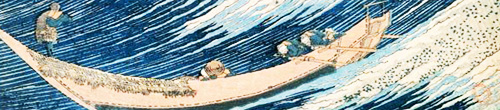
\includegraphics[width=.9\linewidth]{wave}} 

\author{%
\begin{tabular}{c}
	Gabriel Peyr{\'e} \\ CNRS \& DMA \\
	 \'Ecole Normale Sup\'erieure \\
	 \url{gabriel.peyre@ens.fr}\\
	 \url{www.gpeyre.com}\\
	 \url{www.numerical-tours.com}
\end{tabular}
}


\date{\today}

%%

\begin{document}

\maketitle

% !TEX root = ../IntroImaging.tex

\chapter*{Presentation}


The four chapters of this text are independent and present gentle introductions to a few important mathematical foundations of data sciences:
\begin{itemize}
	\item Chapter~\ref{chap-shannon} presents Shannon theory of compression, and insists in particular on the entropy bound for coding of information.
	\item Chapter~\ref{chap-images} presents the basics of image processing, in particular some important processings (quantization, densoising, colors).
	\item Chapter~\ref{chap-sparsity} presents sampling theory, from Shannon classical sampling to compressed sensing. It also serves as a gentle introduction to the field of inverse problems regularization.
	\item Chapter~\ref{chap-ot} presents optimal transport and its applications to data sciences.
\end{itemize}
The exposition level for the first two chapters is elementary. The last chapter presents more advanced mathematical concepts and results. 


\tableofcontents
% !TEX root = ../FundationsDataScience.tex

\chapter{Shannon Theory}
\label{sec-shannon}

%
Shannon theory of information, published in 1948/1949, is made of three parts:
\begin{enumerate}
	\item Sampling: it studies condition under which sampling a continuous function to obtain a discrete vector is invertible. The discrete real values representing the signal are then typically quantized to a finite precision to obtain a set of symbols in a finite alphabet.  
	\item Source coding: it studies optimal ways to represent (code) such a set of symbols as a binary sequence. It leverages the statistical distributions to obtain the most possible compact code.  
	\item Channel coding (not studied here): it studies how to add some redundancy to the coded sequence in order to gain robustness to errors or attacks during transmission (flip of certain bits with some probability). It is often named ``error correcting codes theory''. 
\end{enumerate}
%
The main reference for this chapter is~\cite{mallat2008wavelet}.


%%%%%%%%%%%%%%%%%%%%%%%%%%%%%%%%%%%%%%%%%%%%%%%%%%%%%%%%%%%%%%%%%%%%
%%%%%%%%%%%%%%%%%%%%%%%%%%%%%%%%%%%%%%%%%%%%%%%%%%%%%%%%%%%%%%%%%%%%
%%%%%%%%%%%%%%%%%%%%%%%%%%%%%%%%%%%%%%%%%%%%%%%%%%%%%%%%%%%%%%%%%%%%
\section{Analog vs. Discrete Signals}

To develop numerical tools and analyze their performances, the mathematical modelling is usually done over a continuous setting (so-called ``analog signals''). 
%
Such continuous setting also aims at representing the signal in the physical world, which are inputs to sensors hardwares such as microphone, digital cameras or medical imaging devices. 
%
An analog signal is a 1-D function $f_0 \in \Ldeux([0,1])$ where $[0,1]$ denotes the domain of acquisition, which might for instance be time. An analog image is a 2D function $f_0 \in \Ldeux([0,1]^2)$ where the unit square $[0,1]^2$ is the image domain.

Although these notes are focussed on the processing of sounds and natural images, most of the methods extend to multi-dimensional datasets, which are higher dimensional mappings
\eq{
	f_0 : [0,1]^d \rightarrow [0,1]^s
}
where $d$ is the dimensionality of the input space ($d=1$ for sound and $d=2$ for images) whereas $s$ is the dimensionality of the feature space. For instance, gray scale images corresponds to $(d=2,s=1)$, 
videos to $(d=3, s=1)$, color images to $(d=2, s=3)$ where one has three channels $(R,G,B)$.
One can even consider multi-spectral images where $(d=2, s \gg 3)$ that is made of a large number of channels for different light wavelengths. Figures \ref{fig-examples-1} and \ref{fig-examples-2} show examples of such data.


\myfigure{
	\image{orthobases}{.35}{example-sound}
	\image{orthobases}{.28}{example-image}
	\image{orthobases}{.3}{example-video}
}{%
	Examples of sounds ($d=1$), image ($d=2$) and videos ($d=3$). %	
}{fig-examples-1}

\myfigure{
	\image{orthobases}{.4}{example-color}
	\image{orthobases}{.5}{example-multispectral}
}{%
	Example of color image $s=3$ and multispectral image ($s=32$). %	
}{fig-examples-2}


%%%%%%%%%%%%%%%%%%%%%%%%%%%%%%%%%%%%%%%%%%%
\subsection{Acquisition and Sampling}

Signal acquisition is a low dimensional projection of the continuous signal performed by some hardware device. This is for instance the case for a microphone that acquires 1D samples or a digital camera that acquires 2D pixel samples.
The sampling operation thus corresponds to mapping from the set of continuous functions to a discrete finite dimensional vector with $N$ entries.
\eq{
	f_0 \in \Ldeux([0,1]^d) \mapsto f \in \CC^N
}

\myfigure{
	\image{orthobases}{.4}{discretization-image}
	\image{orthobases}{.5}{discretization-sound}
}{%
	Image and sound discretization. %	
}{fig-discretization}

Figure \ref{fig-discretization} shows examples of discretized signals.

%%%%%%%%%%%%%%%%%%%%%%%%%%%%%%%%%%%%%%%%%%%
\subsection{Linear Translation Invariant Sampler}

A translation invariant sampler performs the acquisition as an inner product between the continuous signal and a constant impulse response $h$ translated at the sample location
\eql{\label{eq-linear-sampling}
	f_n = \int_{-S/2}^{S/2} f_0(x) h(n/N - x) \d x= f_0 \star h(n/N).
}
The precise shape of $h(x)$ depends on the sampling device, and is usually a smooth low pass function that is maximal around $x=0$. The size $S$ of the sampler determines the precision of the sampling device, and is usually of the order of $1/N$ to avoid blurring (if $S$ is too large) or aliasing (if $S$ is too small).

Section \ref{sec-sampling} details how to reverse the sampling operation in the case where the function is smooth.


%%%%%%%%%%%%%%%%%%%%%%%%%%%%%%%%%%%%%%%%%%%%%%%%%%%%%%%%%%%%%%%%%%%%
%%%%%%%%%%%%%%%%%%%%%%%%%%%%%%%%%%%%%%%%%%%%%%%%%%%%%%%%%%%%%%%%%%%%
%%%%%%%%%%%%%%%%%%%%%%%%%%%%%%%%%%%%%%%%%%%%%%%%%%%%%%%%%%%%%%%%%%%%
\section{Shannon Sampling Theorem}
\label{subsec-sampling}

%%%
\paragraph{Reminders about Fourier transform.}

For $f \in L^1(\RR)$, its Fourier transform is defined as
\eql{\label{eq-fourier-transform}
	\foralls \om \in \RR, \quad
	\hat f(\om) \eqdef \int_\RR f(x) e^{-\imath x \om} \d x.
}
One has $\norm{\hat f}^2 = (2\pi)^{-1} \norm{f}^2$, so that $f \mapsto \hat f$ can be extended by continuity to $L^2(\RR)$, which corresponds to computing $\hat f$ as a limit when $T \rightarrow +\infty$ of $\int_{-T}^T f(x) e^{-\imath x \om} \d x$.
%
When $\hat f \in L^1(\RR)$, one can invert the Fourier transform so that
\eql{\label{eq-i-ft}
	f(x) = \frac{1}{2\pi} \int_\RR \hat f(\om) e^{\imath x \om} \d \om, 
}
which shows in particular that $f$ is continuous with vanishing limits at $\pm\infty$. 

The Fourier transform $\Ff : f \mapsto \hat f$ exchanges regularity and decay. For instance, if $f \in C^p(\RR)$ with an integrable Fourier transform, then $\Ff(f^{(p)})(\om) = (\imath \om)^{p} \hat f(\om)$ so that $|\hat f(\om)|=O(1/|\om|^p)$. 
%
Conversely, 
\eql{\label{eq-fourier-regul}
	\int_\RR (1+|\om|)^{p} |\hat f(\om)| \d \om<+\infty
	\qarrq f \in C^p(\RR).
}
For instance, if $\hat f(\om)=O(1/|\om|^{p+2})$, one obtains that $f \in C^p(\RR)$. 

%%%
\paragraph{Reminders about Fourier series.}

We denote $\TT=\RR/2\pi\ZZ$ the torus.
%
A function $f \in L^2(\TT)$ is $2\pi$-periodic, and can be viewed as a function $f \in L^2([0,2\pi])$ (beware that this means that the boundary points are glued together), and its Fourier coefficients are
\eq{
	\foralls n \in \ZZ, \quad 
	\hat f_n \eqdef \frac{1}{2\pi}\int_0^{2\pi} f(x) e^{-\imath x n} \d x.
}
This formula is equivalent to the computation of an inner-product $\hat f_n = \dotp{f}{e_n}$ for the inner-product $\dotp{f}{g} \eqdef \frac{1}{2\pi} \int_\TT f(x) \bar g(x) \d x$. 
%
For this inner product, $(e_n)_n$ is orthonormal and is actually an Hilbert basis, meaning that one reconstructs with the following converging series 
\eql{\label{eq-fourier-series}
	f = \sum_{n \in \ZZ} \dotp{f}{e_n} e_n
}
which means $\norm{f-\sum_{n=-N}^N \dotp{f}{e_n} e_n}_{L^2(\TT)} \rightarrow 0$ for $N \rightarrow +\infty$.
%
The pointwise convergence of~\eqref{eq-fourier-series} at some $x \in \TT$ is ensured if for instance $f$ is differentiable. The series is normally convergent (and hence uniform) if for instance $f$ if of class $C^2$ on $\TT$ sin ce in this case, $\hat f_n = O(1/n^2)$. 
%
If there is a step discontinuities, then there is Gibbs oscillations preventing uniform convergence, but the series still converges to the half of the left and right limit.


%%%
\paragraph{Poisson formula.}

The poisson formula connects the Fourier transform and the Fourier series to sampling and periodization operators.
%
For some function $h(t)$ defined on $\RR$ (typically the goal is to apply this to $h=\hat f$), its periodization reads
\eql{\label{eq-periodizing}
	h_P(t) \eqdef \sum_n h(t-2\pi n).
} 
This formula makes sense if $h \in L^1(\RR)$, and in this case $\norm{h_P}_{L^1(\TT)} \leq \norm{h}_{L^1(\RR)}$ (and there is equality for positive functions). 
%
The Poisson formula, stated in Proposition~\ref{prop-poisson} bellow, corresponds to proving that the following diagram
\eq{
	\begin{array}{rcccl}
						& f(x)  &  \overset{\Ff}{\longrightarrow} &  \hat f(\om) &\\
		\text{sampling}& \downarrow & & \downarrow &\text{periodization} \\
						& (f(n))_n  &  \overset{\text{Fourier serie}}{\longrightarrow} &  \sum_n f(n) e^{-\imath \om n} &\\
	\end{array}
}
is actually commutative.

\begin{prop}[Poisson formula]\label{prop-poisson}
Assume that $\hat f$ has compact support and that $|f(x)| \leq C(1+|x|)^{-3}$ for some $C$. Then one has 
\eql{\label{eq-poisson-formula}
	\foralls \om \in \RR, \quad
	\sum_n f(n) e^{-\imath \om n} = \hat f_P(\om).
}
\end{prop}
\begin{proof}
	Since $\hat f$ is compactly supported, $\hat f_P$ is well defined (it involves only a finite sum) and since $f$ has fast decay, using~\eqref{eq-fourier-regul}, $(\hat f)_P$ is $C^1$. It is thus the sum of its Fourier series
	\eql{\label{eq-poisson-formula}
		(\hat f)_P(\om) = \sum_k c_k e^{\imath k \om},
	} 
	where
	\begin{align*}
		c_k = \frac{1}{2\pi} \int_0^{2\pi} (\hat f)_P(\om) e^{-\imath k \om} \d \om = 
		\frac{1}{2\pi} \int_0^{2\pi} \sum_n \hat f(\om-2\pi n) e^{-\imath k \om}  \d \om .
	\end{align*}
	One has 
	\eq{
		\int_0^{2\pi} \sum_n |\hat f(\om-2\pi n) e^{-\imath k \om}|  \d \om = \int_\RR |\hat f| 
	}
	which is bounded because $\hat f \in L^1(\RR)$ (it has a compact support and is $C^1$), so one can exchange the sum and integral
	\eq{
		c_k = \sum_n \frac{1}{2\pi} \int_0^{2\pi} \hat f(\om-2\pi  n) e^{-\imath k \om}  \d \om
		= \frac{1}{2\pi} \int_{\RR} \hat f(\om) e^{-\imath k \om}  \d \om
		= f(-k)
	}
	where we used the inverse Fourier transform formula~\eqref{eq-i-ft}, which is legit because $\hat f \in L^1(\RR)$.
\end{proof}

%%%
\paragraph{Shannon theorem.}

Shannon sampling theorem state a sufficient condition ensuring that the sampling operator $f \mapsto (f(ns))_n$ is invertible for some sampling step size $s>0$. 
%
It require that $\supp(\hat f) \subset [-\pi/s,\pi/s]$, which, thanks to formula~\eqref{eq-i-ft}, implies that $\hat f$ is $C^\infty$ (in fact it is even analytic). 
%
This theorem was first proved by Wittaker in 1915. It was re-proved and put in perspective in electrical engineering by Nyquist in 1928. It became famous after the paper of Shannon in 1949, which put forward its importance in numerical communications.
%
Figure~\ref{fig-sampling-aliasing} give some insight on how the proof works (left) and more importantly, on what happens when the compact support hypothesis fails (in which case aliasing occurs, see also Figure~\ref{fig-aliasing}). 

\myfigure{
	\image{1-shannon}{.8}{sampling-aliasing}
}{%
	Schematic view for the proof of Theorem~\ref{thm-shannon-sampling}. %	
}{fig-sampling-aliasing}





\begin{thm} \label{thm-shannon-sampling}
	If $|f(x)| \leq C(1+|x|)^{-3}$ for some $C$ and $\supp(\hat f) \subset [-\pi/s,\pi/s]$, then one has
	\eql{\label{eq-shannong-interp}
		\foralls x \in \RR, \quad 
		f(x) = \sum_n f(n s) \sinc(x/s-n) \qwhereq
		\sinc(u) = \frac{\sin(\pi u)}{\pi u}
	}
	with uniform convergence.
\end{thm}

\begin{proof} 
	The change of variable $g \eqdef f(s \cdot)$ results in $\hat g=1/s \hat f(\cdot/s)$, indeed, denoting $z=s x$
	\eq{
		\hat g(\om) = \int f(s x) e^{-\imath \om x} \d x = \frac{1}{s} \int f(z) e^{-\imath (\om/s) z} \d z = \hat f(\om/s)/s, 
	} 
	so that we can restrict our attention to $s=1$.
	%
	The compact support hypothesis implies $\hat f(\om) = 1_{[-\pi,\pi]}(\om) \hat f_P(\om)$.  
	Combining the inversion formula~\eqref{eq-i-ft} with Poisson formula~\eqref{eq-poisson-formula}
	\eq{
		f(x) = \frac{1}{2\pi} \int_{-\pi}^\pi \hat f_P(\om) e^{\imath \om x} \d \om
		= \frac{1}{2\pi} \int_{-\pi}^\pi \sum_n f(n) e^{\imath \om (x-n)} \d \om.
	} 
	Since $f$ has fast decay, $\int_{-\pi}^\pi \sum_n |f(n) e^{\imath \om (x-n)}| \d \om = \sum_n |f(n)| < +\infty$, so that one can exchange summation and integration and obtain
	\eq{
		f(x) = \sum_n f(n)  \frac{1}{2\pi} \int_{-\pi}^\pi e^{\imath \om (x-n)} \d \om = \sum_n f(n) \sinc(x-n).
	}
\end{proof}

\wrapf{1-shannon/sinc}{sinc kernel}
One issue with this reconstruction formula is that it uses a slowly decaying and very oscillating $\sinc$ kernels. In practice, one rarely uses such a kernel for interpolation, and one prefers smoother and more localized kernel. If $\supp(\hat f) \subset [-\pi/s',\pi/s']$ with $s'>s$ (i.e. have a more compact spectrum), one can re-do the proof of the theorem, and one gains some degree of freedom to design the reconstruction kernel, which now can be chosen smoother in Fourier and hence have exponential decay in time. 

%
Spline interpolation are defined by considering $\phi_0=1_{[-1/2,1/2]}$ and $\phi_k = \phi_{k-1} \star \phi_0$ which is a piecewise polynomial of degree $k$ and has bounded derivative of order $k$ (and is of class $C^{k-1}$) with compact support on $[-(k+1)/2,(k+1)/2]$. The reconstruction formula reads $f \approx \tilde f \eqdef \sum_n a_n \phi(\cdot-n)$ where $(a_n)_n$ is computed from the $(f(n))_n$ by solving a linear system (associated to the interpolation property $\tilde f(n)=f(n)$). It is only in the cases $k \in \{0,1\}$ (piecewise constant and affine interpolations) that one has $a_n=f(n)$.
%
In practice, one typically use the cubic spline interpolation, which corresponds to $k=3$.

\texttt{Associated code: test\_sampling.m}

\myfigure{
	\image{1-shannon}{.6}{spline}
}{%
	Cardinal splines as bases functions for interpolation. %	
}{fig-aliasing}



This theorem also explains what happens if $\hat f$ is not supported in $[-\pi/s,\pi/s]$. This leads to aliasing, and high frequency outside this interval leads to low frequency artifacts often referred to as ``aliasing''. If the input signal is not bandlimitted, it is thus very important to pre-filter it (smooth it) before sampling to avoid this phenomena (of course this kills the high frequencies, which are lost), see Figure~\ref{fig-aliasing}. 

\myfigure{
	\image{1-shannon}{.6}{aliasing}
}{%
	Aliasing in the simple case of a sine wave (beware however that this function does not have compact support). %	
}{fig-aliasing}

%%%
\paragraph{Quantization.}

Once the signal have been sampled to obtain a discrete vector, in order to store it and transmit it, it is necessary to quantize the value to some finite precision. 
% 
Section~\ref{sec-transform-coding} presents transform coding, which is an efficient family of compression schemes which operate the quantization over some transformed domain (which correspond to applying a linear transform, usually orthogonal, to the sampled values). This is useful to enhance the performance of the source coding scheme. It is however common to operate directly the quantization over the sampled value. 

Considering for instance a step size $s=1/N$, one samples $(u_n \eqdef f(n/N))_{n=1}^{N} \in \RR^N$ to obtain a finite dimensional data vector of length $N$. Note that dealing with finite data corresponds to restricting the function $f$ to some compact domain (here $[0,1]$) and is contradictory with Shannon sampling theorem, since a function $f$ cannot have a compact support in both space and frequency (so perfect reconstruction never holds when using finite storage).

\wrapf{1-shannon/quantizer}{}

Choosing a quantization step $T$, quantization $v_n = Q_T(u_n) \in \ZZ$ rounds to the nearest multiple of $T$, i.e. 
\eq{
	v = Q_T(u) \quad\Leftrightarrow\quad
	v-\frac{1}{2} \leq u/T < v+\frac{1}{2},
}
see Fig.~\ref{fig-quantizer}. De-quantization is needed to restore a signal, and the best reconstruction (in average or in worse case) is defined by setting $D_T(v) \eqdef T v$. Quantizing and then de-quantizing introduce an error bounded by $T/2$, since $|D_T(Q_T(u))-u| \leq T/2$. 
%
Up to machine precision, quantization is the only source of error (often called ``lossy compression'') in Shannon's standard pipeline.


\myfigure{
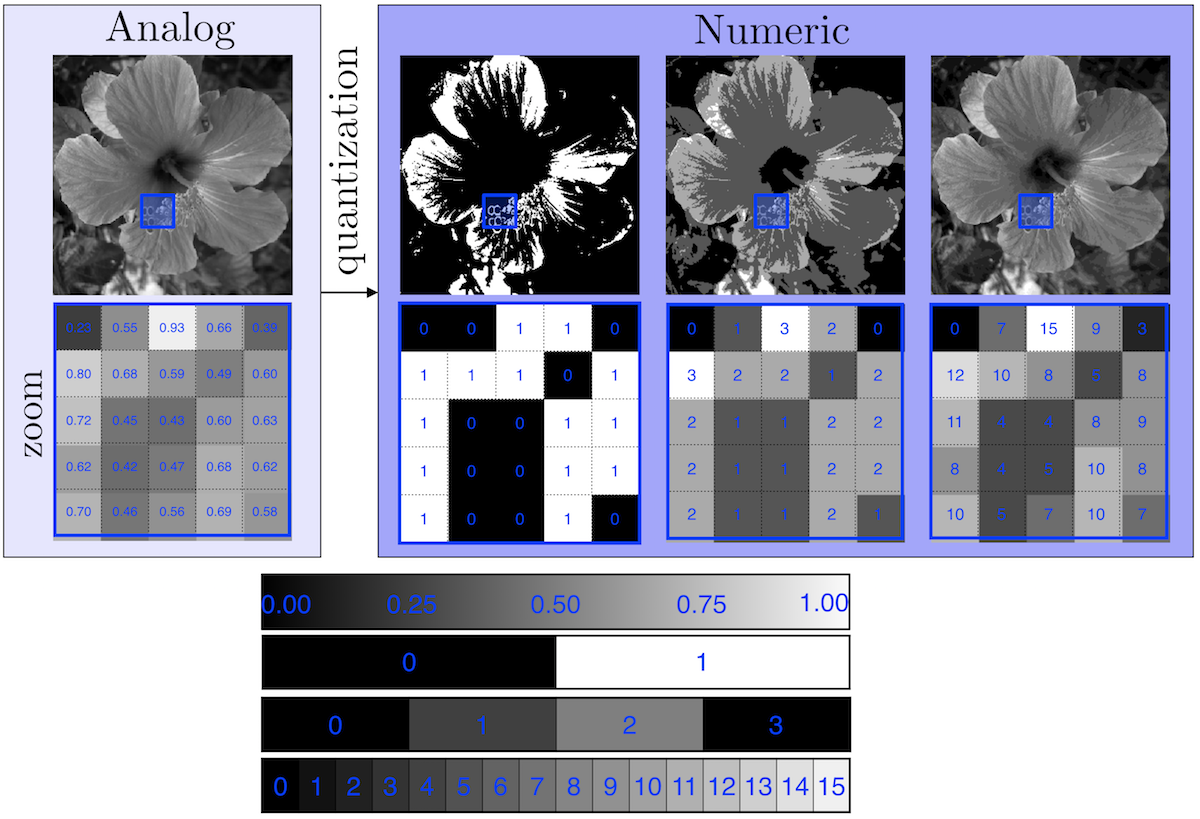
\includegraphics[width=.8\linewidth]{1-shannon/quantize/quantization}
%\tabquatre{
%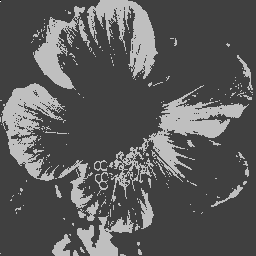
\includegraphics[width=.2\linewidth]{1-shannon/quantize/quantize-2}&
%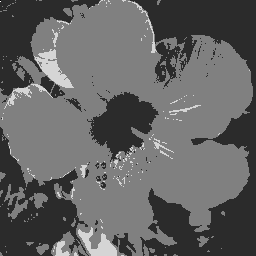
\includegraphics[width=.2\linewidth]{1-shannon/quantize/quantize-3}&
%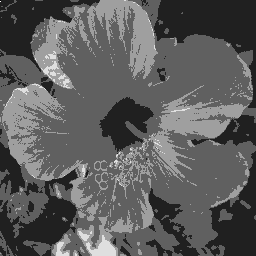
\includegraphics[width=.2\linewidth]{1-shannon/quantize/quantize-4}&
%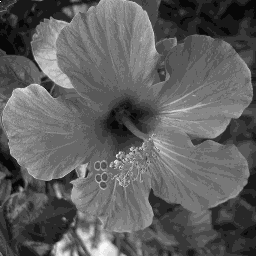
\includegraphics[width=.2\linewidth]{1-shannon/quantize/quantize-16}\\
%$2$ graylevels &
%$3$ graylevels &
%$4$ graylevels &
%$16$ graylevels 
%}
}{Quantizing an image using a decaying $T=1/K$ where $K \in \{2,3,4,16\}$ is the number of graylevels and the original image is normalized so that $0 \leq f_0 < 1$. 
}{fig-section3-quantize}

%%%%%%%%%%%%%%%%%%%%%%%%%%%%%%%%%%%%%%%%%%%%%%%%%%%%%%%%%%%%%%%%%%%%
\section{Shannon Source Coding Theorem}
\label{sec-shannon-source}

\newcommand{\Symb}{s}

%%%
\paragraph{Uniform coding.}

We consider an alphabet $(\Symb_1,\ldots,\Symb_K)$ of $K$ symbols. For instance, if one samples and quantize a bounded signal $0 \leq f_0 < 1$ using a step size $1/K$, then one can consider $\Symb_k=k$ to be integer symbols. For text, these symbols include the letter plus extra punctuation symbols and blank. 
%
It is of course possible to code a sequence of such symbols using a uniform code (e.g. using the base 2 expansion) with $\lceil \log_2(K) \rceil$ bit per symbols.
For instance if $K=4$ and the symbols are $\{0,1,2,3\}$, then the code words are $(c_0=00,c_1=01,c_2=10,c_3=11)$. 

This uniform coding strategy is however extremely inefficient if the symbols are not uniformly distributed (i.e. if some symbols are more frequent than other, which is likely to be the case). We aim at designing better codes.

%%%
\paragraph{Prefix coding.}
 

A code $c_k=c(\Symb_k)$ associate to each symbol $\Symb_k$ a code word $c_k \in \{0,1\}^\NN$ with a varying length $|c_k| \in \NN^*$. 
%
A prefix code $c_k=c(\Symb_k)$ is such that no word $c_k$ is the beginning of another word $c_k'$. This is equivalent to be able to embed the $(c_k)_k$ as leaves of a binary tree $T$, with the code being output of a traversal from root to leaves (with a convention that going to a left (resp. right) child output a 0 (resp. a 1). 
%
We denote $c=\text{Leaves}(T)$ such prefix property. 


\myfigure{
\image{1-shannon}{.35}{tree/prefix-coding}
\qquad
\image{1-shannon}{.35}{tree/tree-example}
}{%
Left: complete tree of all codes of length 3; right: example of prefix code.
}{fig-tree-prefix}

This tree-based representation is useful to decode a binary stream by simply performing tree traversal. One follows the tree, from top to bottom, and outputs a symbol each time a leaf is reached (and then re-start at the top). 

The following fundamental lemma describes the set of prefix codes using an inequality.

\begin{lem}[Kraft inequality]\label{lem-kraft}
	(i) For a code $c$, if there exists a tree $T$ such that $c=\text{Leaves}(T)$ then
	\eql{\label{eq-kraft-ineg}
		\sum_k 2^{-|c_k|} \leq 1.
	}
	(ii) Conversely, if $(\ell_k)_k$ are such that
	\eql{\label{eq-kraft-ineg-2}
		\sum_k 2^{-\ell_k} \leq 1
	}
	then there exists a code $c=\text{Leaves}(T)$ such that $|c_k|=\ell_k$.
\end{lem} 

\begin{proof}
	$\Rightarrow$ We suppose $c=\text{Leaves}(T)$. We denote $m=\max_k |c_k|$ and consider the full binary tree.
	%
	Bellow each $c_k$, one has a sub-tree of height $m-|c_k|$, see Figure~\ref{fig-fourier-wav}, left. This sub-tree has $2^{m-|c_k|}$ leaves. Since all these sub-trees do not overlap, the total number of leaf do not exceed the total number of leaves $2^m$ of the full binary tree, hence
	\eq{
		\sum_k 2^{m-|c_k|} \leq 2^m, 
	}
	hence~\eqref{eq-kraft-ineg}. 
	
	\myfigure{
	\image{1-shannon}{.35}{kraft-ineq-1}\quad
	\image{1-shannon}{.45}{kraft-ineq-2}
}{%
	Left: full binary tree obtained by completing the tree associated to the code $(c_1=0, c_2=10, c_3=110, c_4=111)$. 
	%
	Right: packing sub-trees associated to code length to form the left part of the full tree. %	
}{fig-fourier-wav}

	
	$\Leftarrow$ Conversely, we assume~\eqref{eq-kraft-ineg} holds. Without loss of generality, we assume that $|c_1| \geq \ldots \geq |c_K|$. We start by putting a sub-tree of height $2^{m-|c_1|}$. Since the second tree is smaller, one can put it immediately aside, and continue this way, see Figure~\ref{fig-fourier-wav}, right. Since  $\sum_k 2^{m-|c_k|} \leq 2^m$, this ensure that we can stack side-by-side all these sub-tree, and this defines a proper sub-tree of the full binary tree. 
\end{proof}


%%
\paragraph{Probabilistic modeling.}

We aim at designing the most possible compact code $c_k$. 
%
We assume at our disposal some probability distribution over this alphabet, which is just an histogram $p=(p_1,\ldots,p_K) \in \RR_+^K$ in the simplex, i.e. $\sum_k p_k=1$. 
%
In practice, this probability is usually the empirical probability of appearance of the symbols $x_k$ in the data to be coded. 

\wrapf{1-shannon/entropie/entropie-fonction}{}

The entropy of such an histogram is 
\eq{
	H(p) \eqdef -\sum_k p_k \log_2(p_k)
}
with the convention $0\log_2(0)=0$. 

Denoting $h(u)=-u \log(u)$, $h'(u)=-\log(u)-1$, $h''(u)=-1/u<0$ so that $H$ is strictly concave. The definition of the entropy extends to continuous density $f(x)$ for $x$ on some measure space with reference measure $\d x$ (e.g. Lebesgue on $\RR^d$) by setting $H(f)=-\int f(x) \log(f(x)) \d x$. 

\myfigure{
\tabquatre{
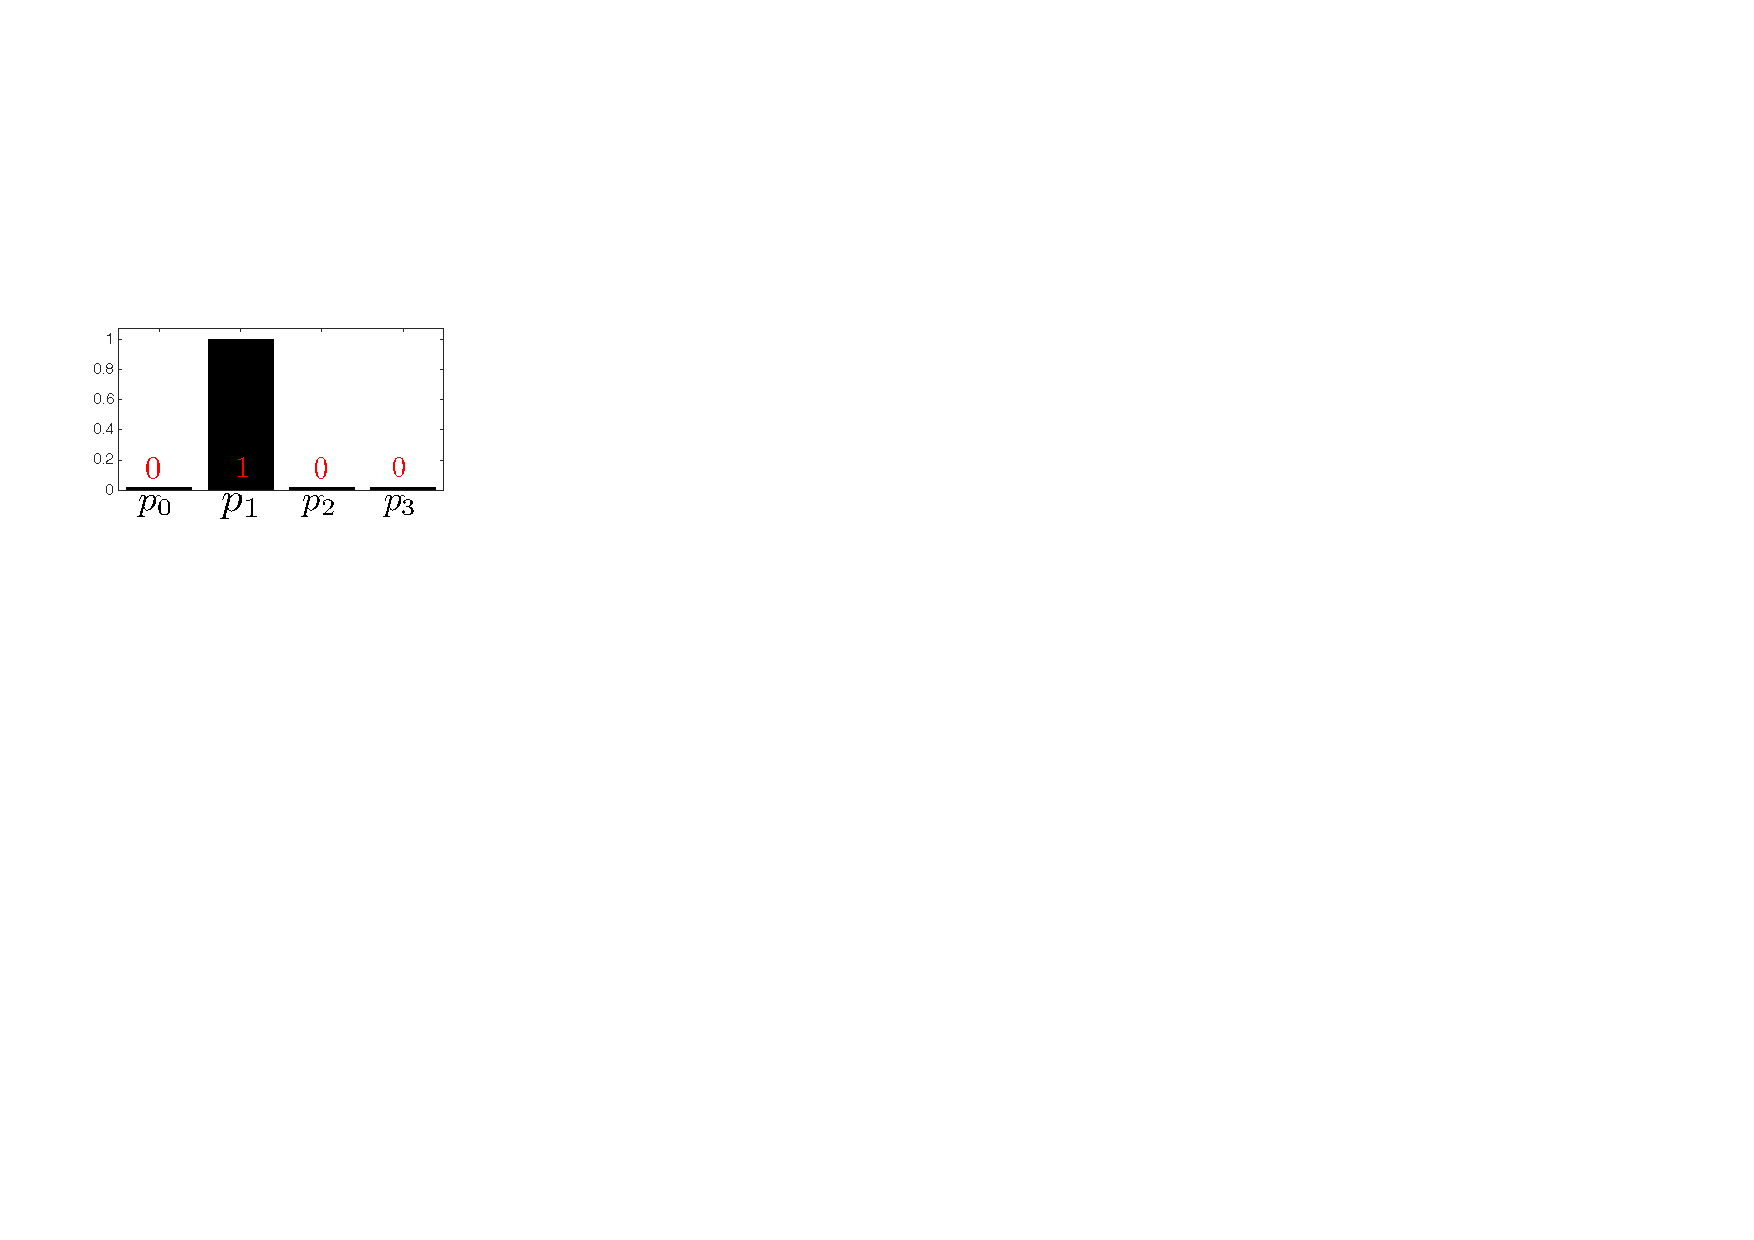
\includegraphics[width=.25\linewidth]{1-shannon/entropie/histo-1}&
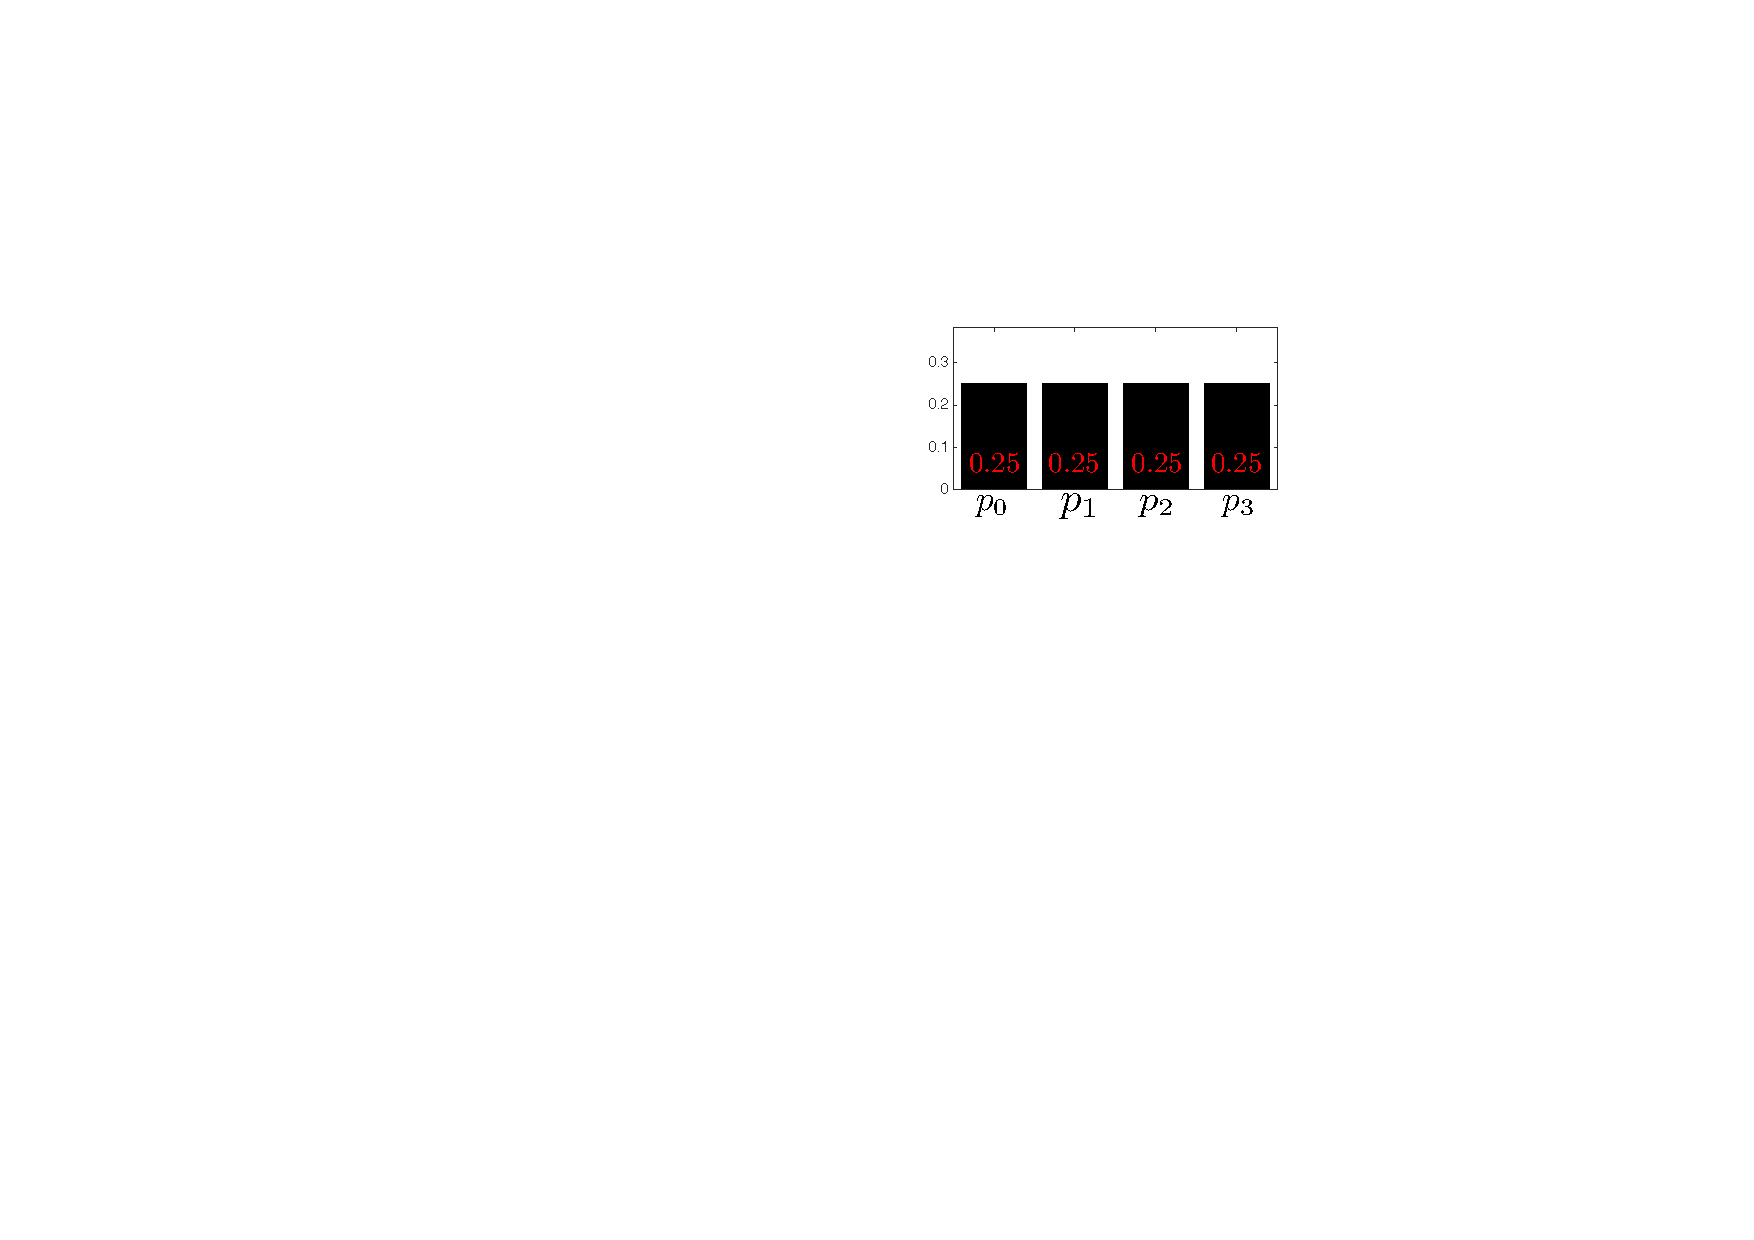
\includegraphics[width=.25\linewidth]{1-shannon/entropie/histo-3}&
\includegraphics[width=.25\linewidth]{1-shannon/entropie/histo-sub}\\
$H(p)=0$ & $H(p)=\log_2(2)=1$ &  $H(p) = 1.62$
}
}{Three examples of probability distributions with corresponding entropies.}{fig-histo-entropy}


\myfigure{
	\image{1-shannon}{.35}{entropy-extrema}
}{%
	Linked extra for the entropy. %	
}{fig-entropy-extrema}



\begin{lem} One has
\eq{
	0 \leq H(p) \leq \log_2(K).
}
\end{lem}


\begin{proof}
	We consider the following constrained optimization problem
	\eq{
		\min_p \enscond{ f(p) }{ g(p) = \sum_k p_k =1 }
	}
	where $f=-H$, see Fig.~\ref{fig-entropy-extrema}. According to the linked extrema theorem, at an optimum $p^\star$, $\nabla f(p^\star)=\la \nabla g(p^\star)$ for some $\la \in \RR$, so that here $\log(p_k^\star)+1 = \la$, i.e. $p_k^\star=c$ is constant, and since 
	$\sum_k p_k^\star=1$, 	
	one has $p_k^*=1/K$ and thus $H(p)=\log_2(K)$.
\end{proof}


%%
\paragraph{Shannon theorem.}

%
Assuming that $(p_k)_k$ is the empirical probability of appearance of the symbols $x_k$ in the data to be coded, the average symbol length associated to some code $c$ is 
\eq{
	L(c) \eqdef \sum_k p_k |c_k|. 
}
The goal is to design the best possible $c$ so that $L(c)$ is as small as possible.
%
Shannon theorem of entropic coding, proved bellow, give both lower and upper bound for this question. 

\begin{thm}
	(i) If $c=\text{Leaves}(T)$ for some tree $T$, then 
	\eq{
		L(c) \geq H(p).
	}
	(ii) Conversely, there exists a code $c$ with $c=\text{Leaves}(T)$ such that 
	\eq{
		L(c) \leq H(p)+1.
	}
\end{thm} 

\begin{proof}
	First, we consider the following optimization problem
	\eql{\label{eq-proof-shannon}
		\umin{ \ell = (\ell_k)_k } \enscond{ f(\ell) \eqdef \sum_k \ell_k p_k }{ g(\ell) \eqdef  \sum_k 2^{-\ell_k} \leq 1 }.
	}
	We fist show that at an optimal $\ell^\star$, the constraint is saturated, i.g. $g(\ell^\star)=1$. Indeed, if $g(\ell^\star)=2^{-u} < 1$, with $u>0$, we define $\ell_k' \eqdef \ell_k^\star-u$, which satisfies $g(\ell') = 1$ and also $f(\ell')=\sum_k (\ell_k-u) p_k < f(\ell^\star)$, which is a contradiction.
	So we can restrict in~\eqref{eq-proof-shannon} the constraint to $g(\ell)=1$ and apply the linked extrema theorem, which shows that necessarily, there exists $\la \in \RR$ with $\nabla f(\ell^\star)=\nabla g(\ell^\star)$, i.e.  $(p_k)_k = -\la \ln(2) (2^{-\ell_k^\star})_k$. Since 
	\eq{
		1 = \sum_k p_k = -\la \ln(2) \sum_k 2^{-\ell_k} = - \la \ln(2) 
	}
	we deduce that $\ell^\star_k = -\log(p_k)$. 
	
	(i) If $c=\text{Leave}(T)$, the by Kraft inequality~\eqref{eq-kraft-ineg}, necessarily $\ell_k=|c_k|$ satisfy the constraints of~\eqref{eq-proof-shannon}, and thus $H(p) = f(\ell^\star) \leq f(\ell) = L(\ell)$.
	
	(ii) We define $\ell_k \eqdef \lceil -\log_2(p_k) \rceil \in \NN^*$. Then $\sum_k 2^{-\ell_k} \leq \sum_k 2^{\log_2(p_k)} = 1$, so that these lengths satisfy~\eqref{eq-kraft-ineg-2}. Thanks to Proposition~\ref{lem-kraft} (ii), there thus exists a prefix code $c$ with $|c_k|=\lceil -\log_2(p_k) \rceil$. Furthermore
	\eq{
		L(c) = \sum_k p_k \lceil -\log_2(p_k) \rceil \leq \sum_k p_k ( -\log_2(p_k) +1) = H(p)+1.
	}
\end{proof}

Note that this proof is constructing, i.e. it gives an algorithm that construct an almost optimal $c$, and this code is often called the Shannon-Fano code. It is usually a good code, although it is not necessarily the optimal code with the smallest $L(c)$. Such an optimal code can easily be computed in almost linear time (only sorting of the probability is needed, so it is $K(\log(K))$) by Huffman's dynamic programming algorithm (invented in 1952). The proof of correctness of this algorithm is however a bit tedious. Figure~\ref{fig-huff-code} shows an example of application of this algorithm.


\texttt{Associated code: coding/test\_text.m}

In practice, such an entropic coding, although optimal, is not very efficient when one of the symbol has a large probability $p_k$. This is because then $2^{-p_k} \ll 1$ but one cannot allocate a fractional number of bit. This is why $L(c)$ can be as large as $H(p)+1$. A simple workaround is to artificially increase the size of the alphabet from $K$ to $K^r$ by grouping together sets of $r$ consecutive symbols, and thus reducing the gap to $H(p)+1/r$. Constructing the code and coding however becomes very slow for large $r$. The standard way to achieve this without explicitly doing the grouping is by using arithmetic coding, invented in 1976, which using interval arithmetic to allocate fractional number of bits and leveraging the fact that one usually code large sequence, thus approaching to arbitrary precision Shannon bound $H(p)$ as the length of the data increases.


\myfigure{
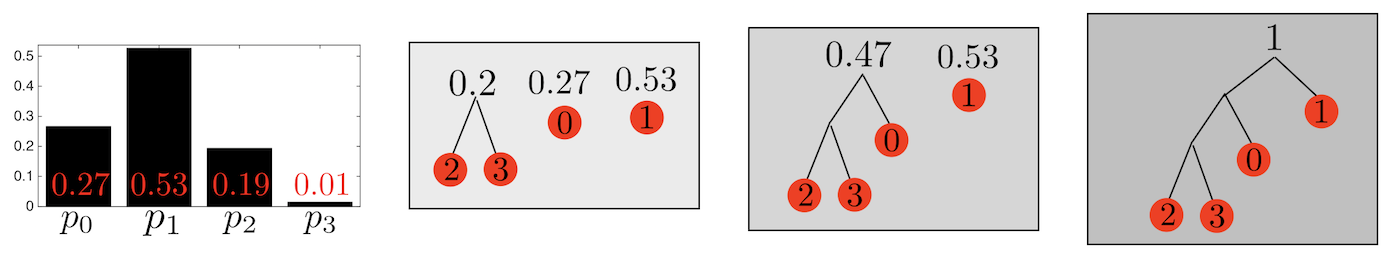
\includegraphics[width=.8\linewidth]{1-shannon/huff-code}
}{Huffman coding algorithm in action.}{fig-huff-code}

Note that while we give some statistical and probabilistic interpretation of entropy (measure of uncertainty) and of Shannon theorem, this theory is fully deterministic and give a bound for the actual length $N L(c)$ of coding some sequence of length $N$ if the probability $p$ are the empirical probability of the sequence.

If one choose a different probability $q$ and use it to code the sequence, one necessarily obtain a worse average coding length, and this is reflected by the positivity of the so-called relative entropy (beware that it is a convex function while the entropy is concave), which is often called the Kulback-Leibler divergence
\eq{
	\text{KL}(p|q) = -\sum_k p_k \log q_k - H(p)   = \sum_k p_k \log \frac{p_k}{q_k} \geq 0.
}
This KL divergence is similar to a distance in the sense that $\text{KL}(p|q)=0$ if and only if $p=q$ (note however that KL is not symmetric and does not satisfies the triangular inequality). It also has the remarkable property that it is jointly convex in $(p,q)$. It is of paramount importance to compare probability distributions and measures, and form the basis of the fields of information theory and information geometry. 


%%
\paragraph{Doing better.}

One can wonder if it is possible to go bellow the entropy bound. By the virtue of Shannon theorem, it is not possible if only can only code in sequential order the symbols themselves. From a statistical perspective, it is as if the symbols where considered to be independent. If there is some redundancy in the sequence of symbol (for instance if they are discretization of a smooth function, so that to consecutive symbols are likely to be equal), it is possible to re-transform (in a bijective way) the sequence to make them ``more independent''. A simple illustration of this idea is given in Figure~\ref{fig-codage-differences}, where one computes successive difference of a 1D sequence of symbols (beware to also retain the initial symbol to be able to do the decoding.

\myfigure{
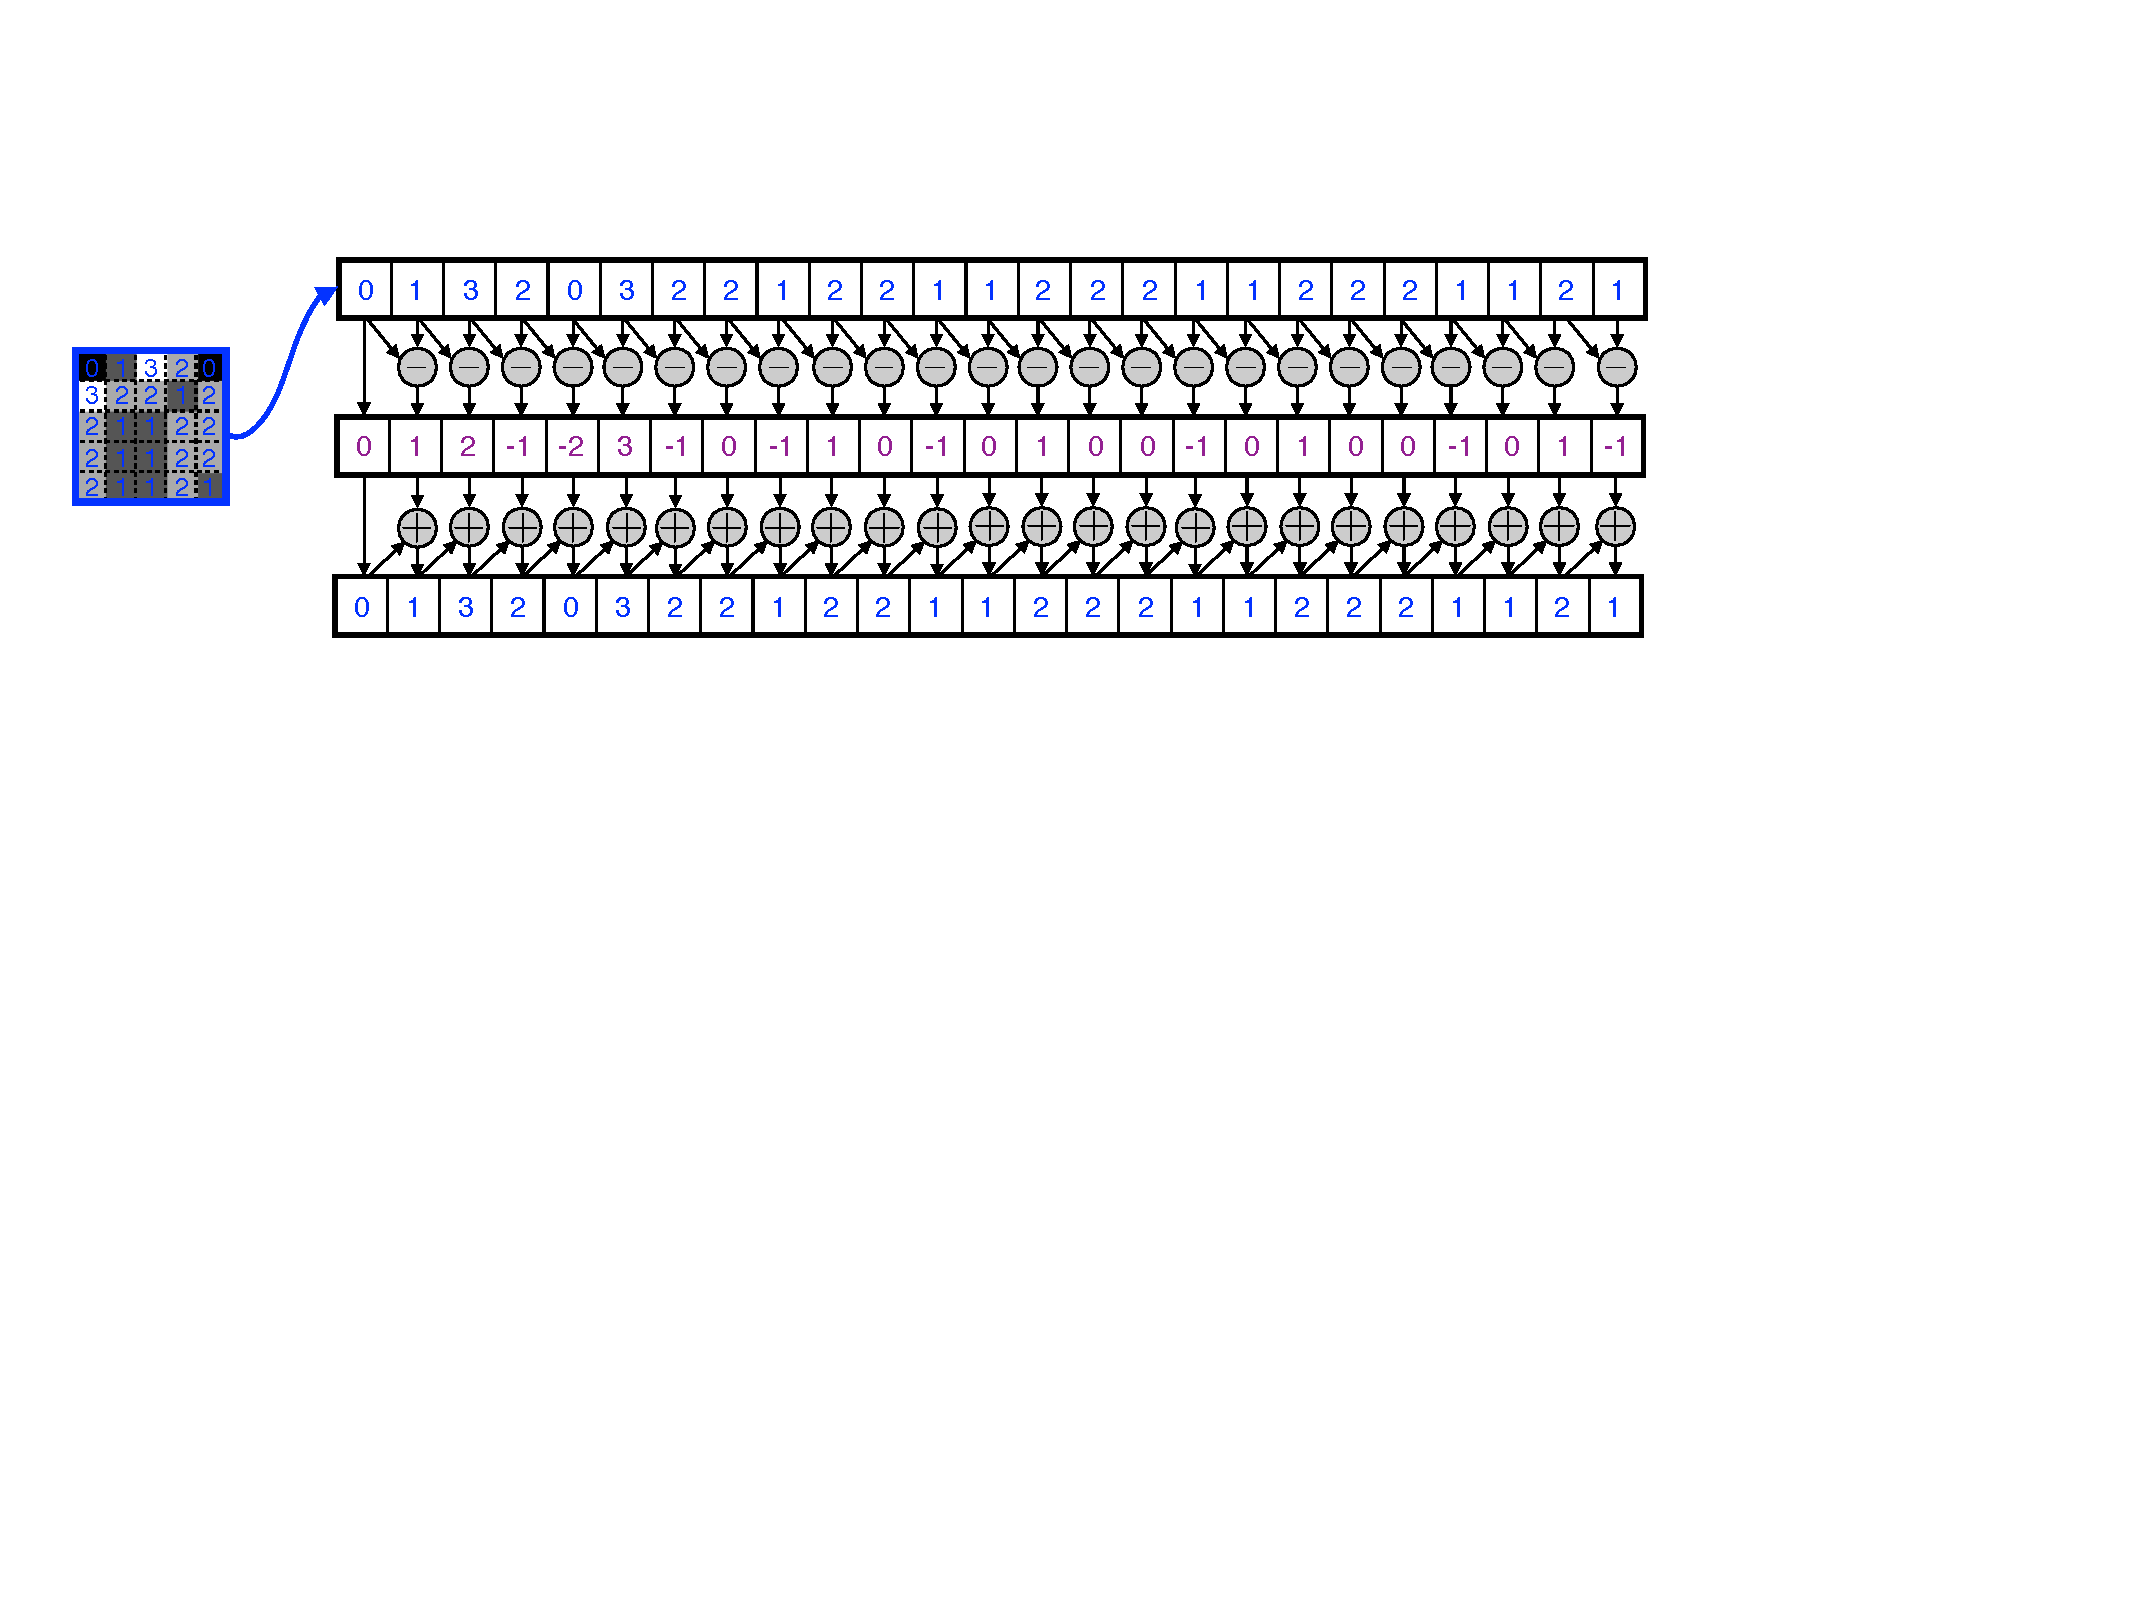
\includegraphics[width=.8\linewidth]{1-shannon/differences/differences}
%
\tabtrois{
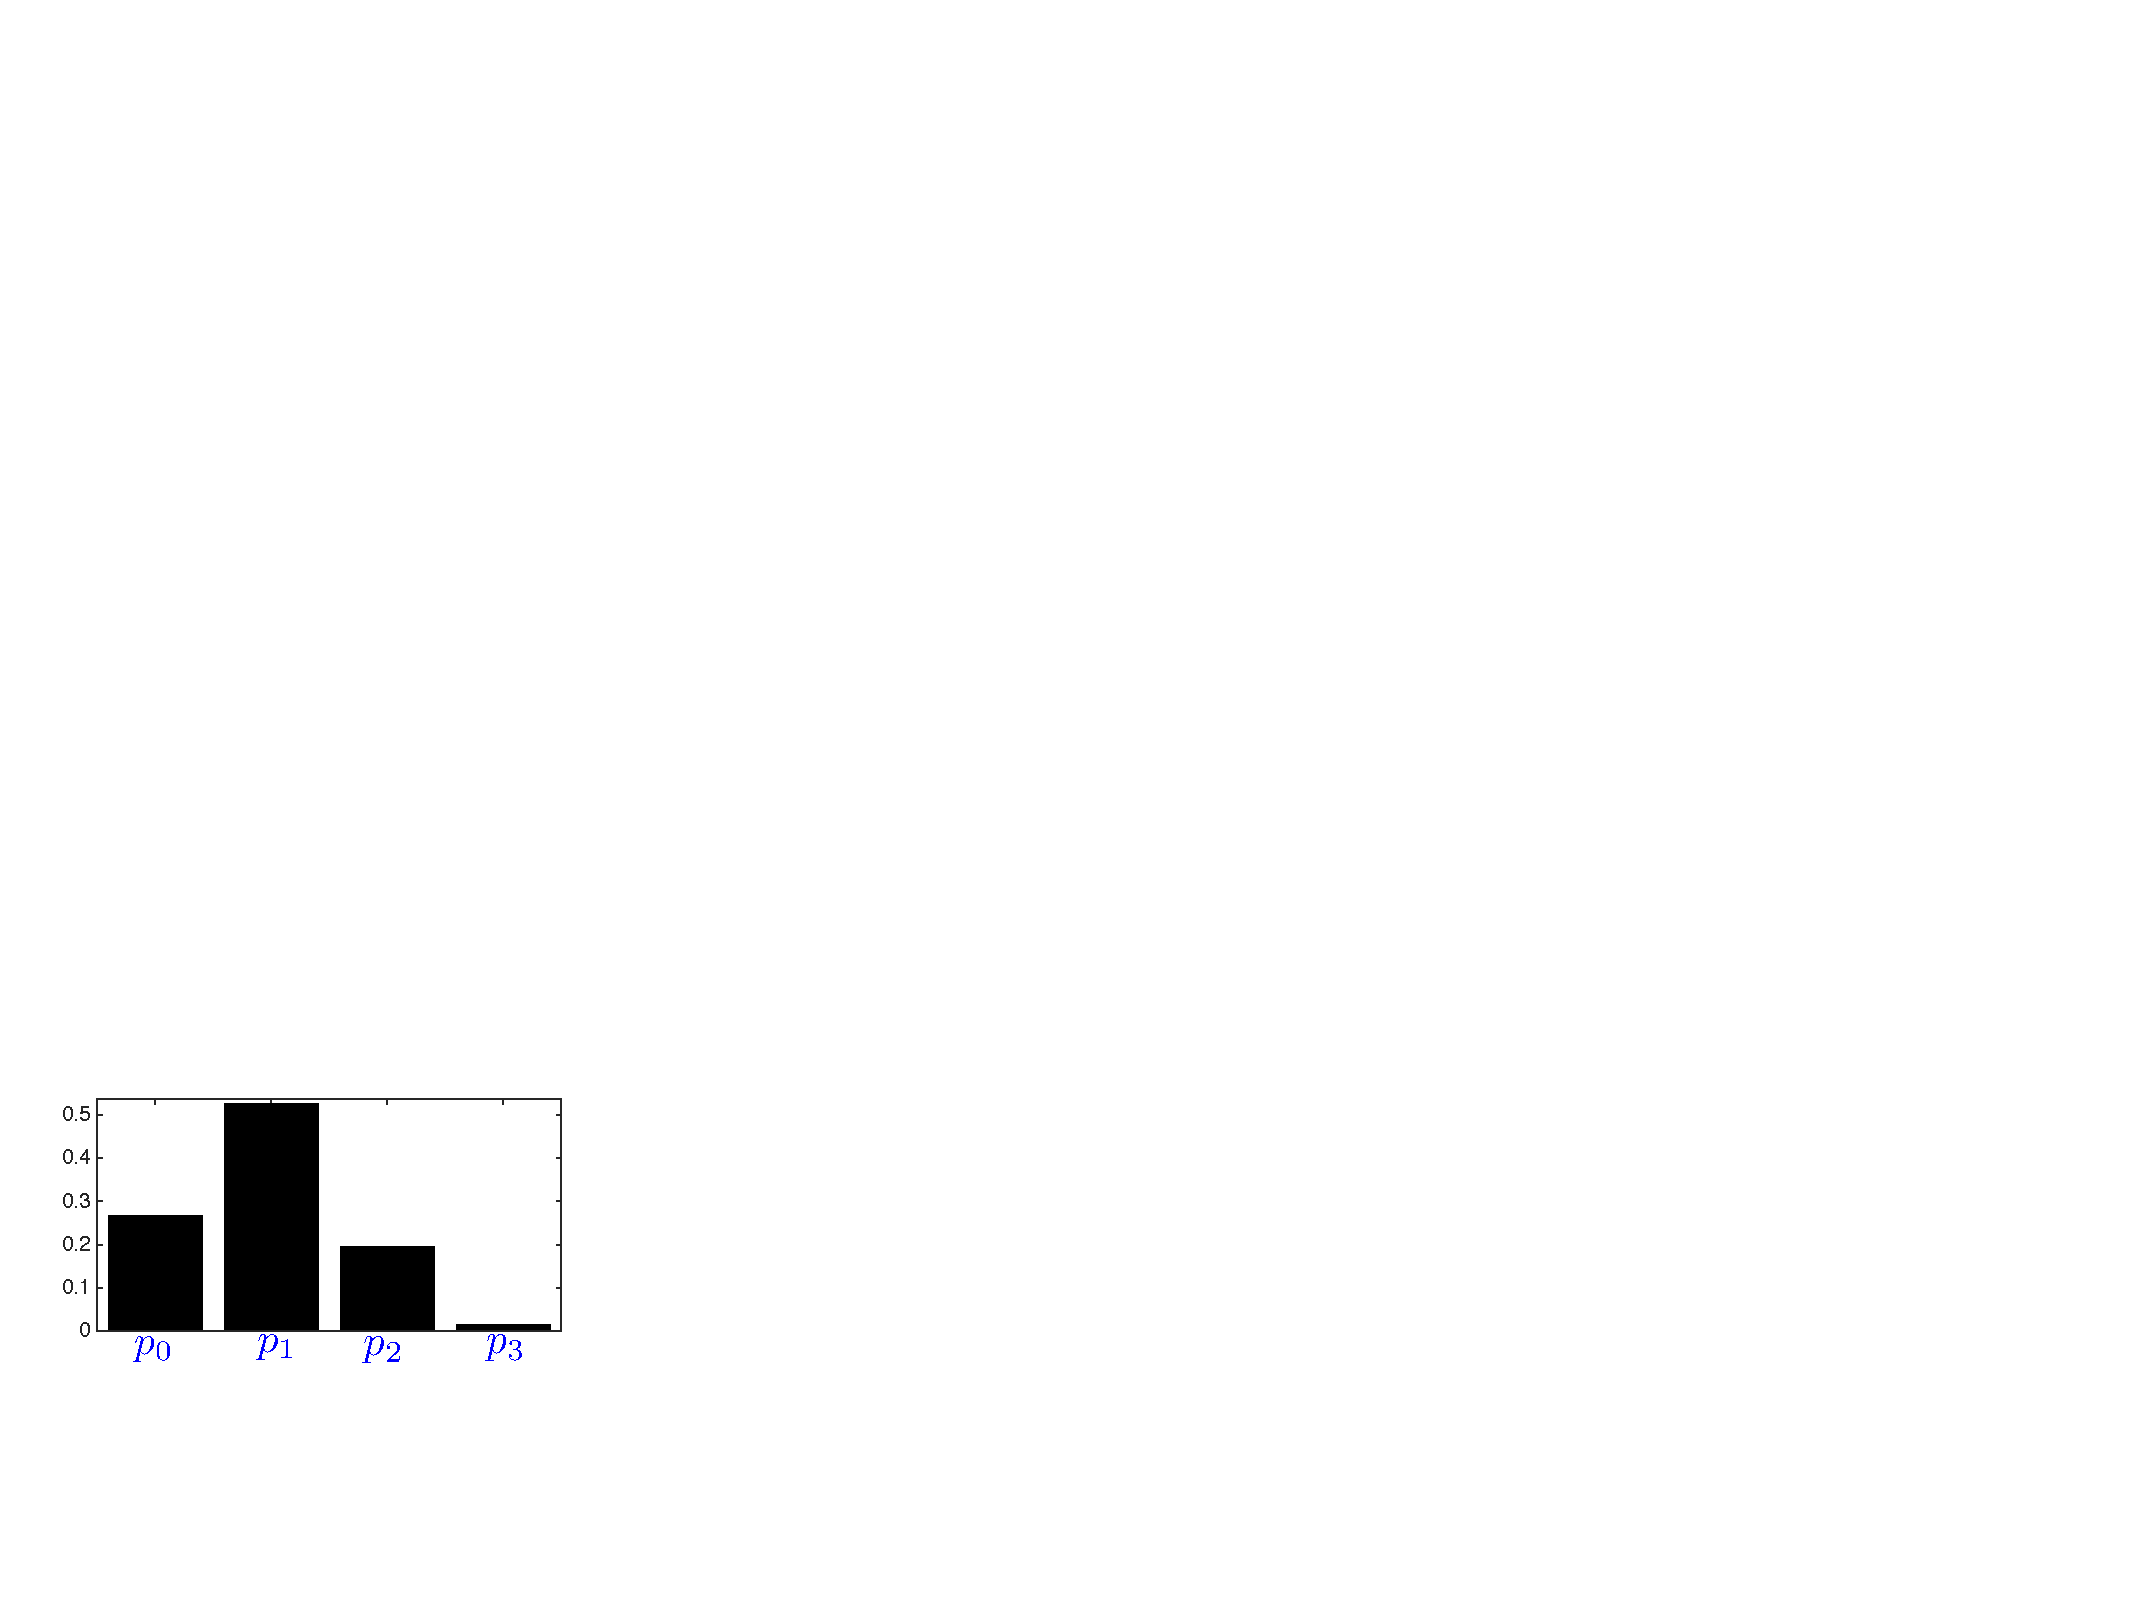
\includegraphics[width=.25\linewidth]{1-shannon/differences/histo-pix}&
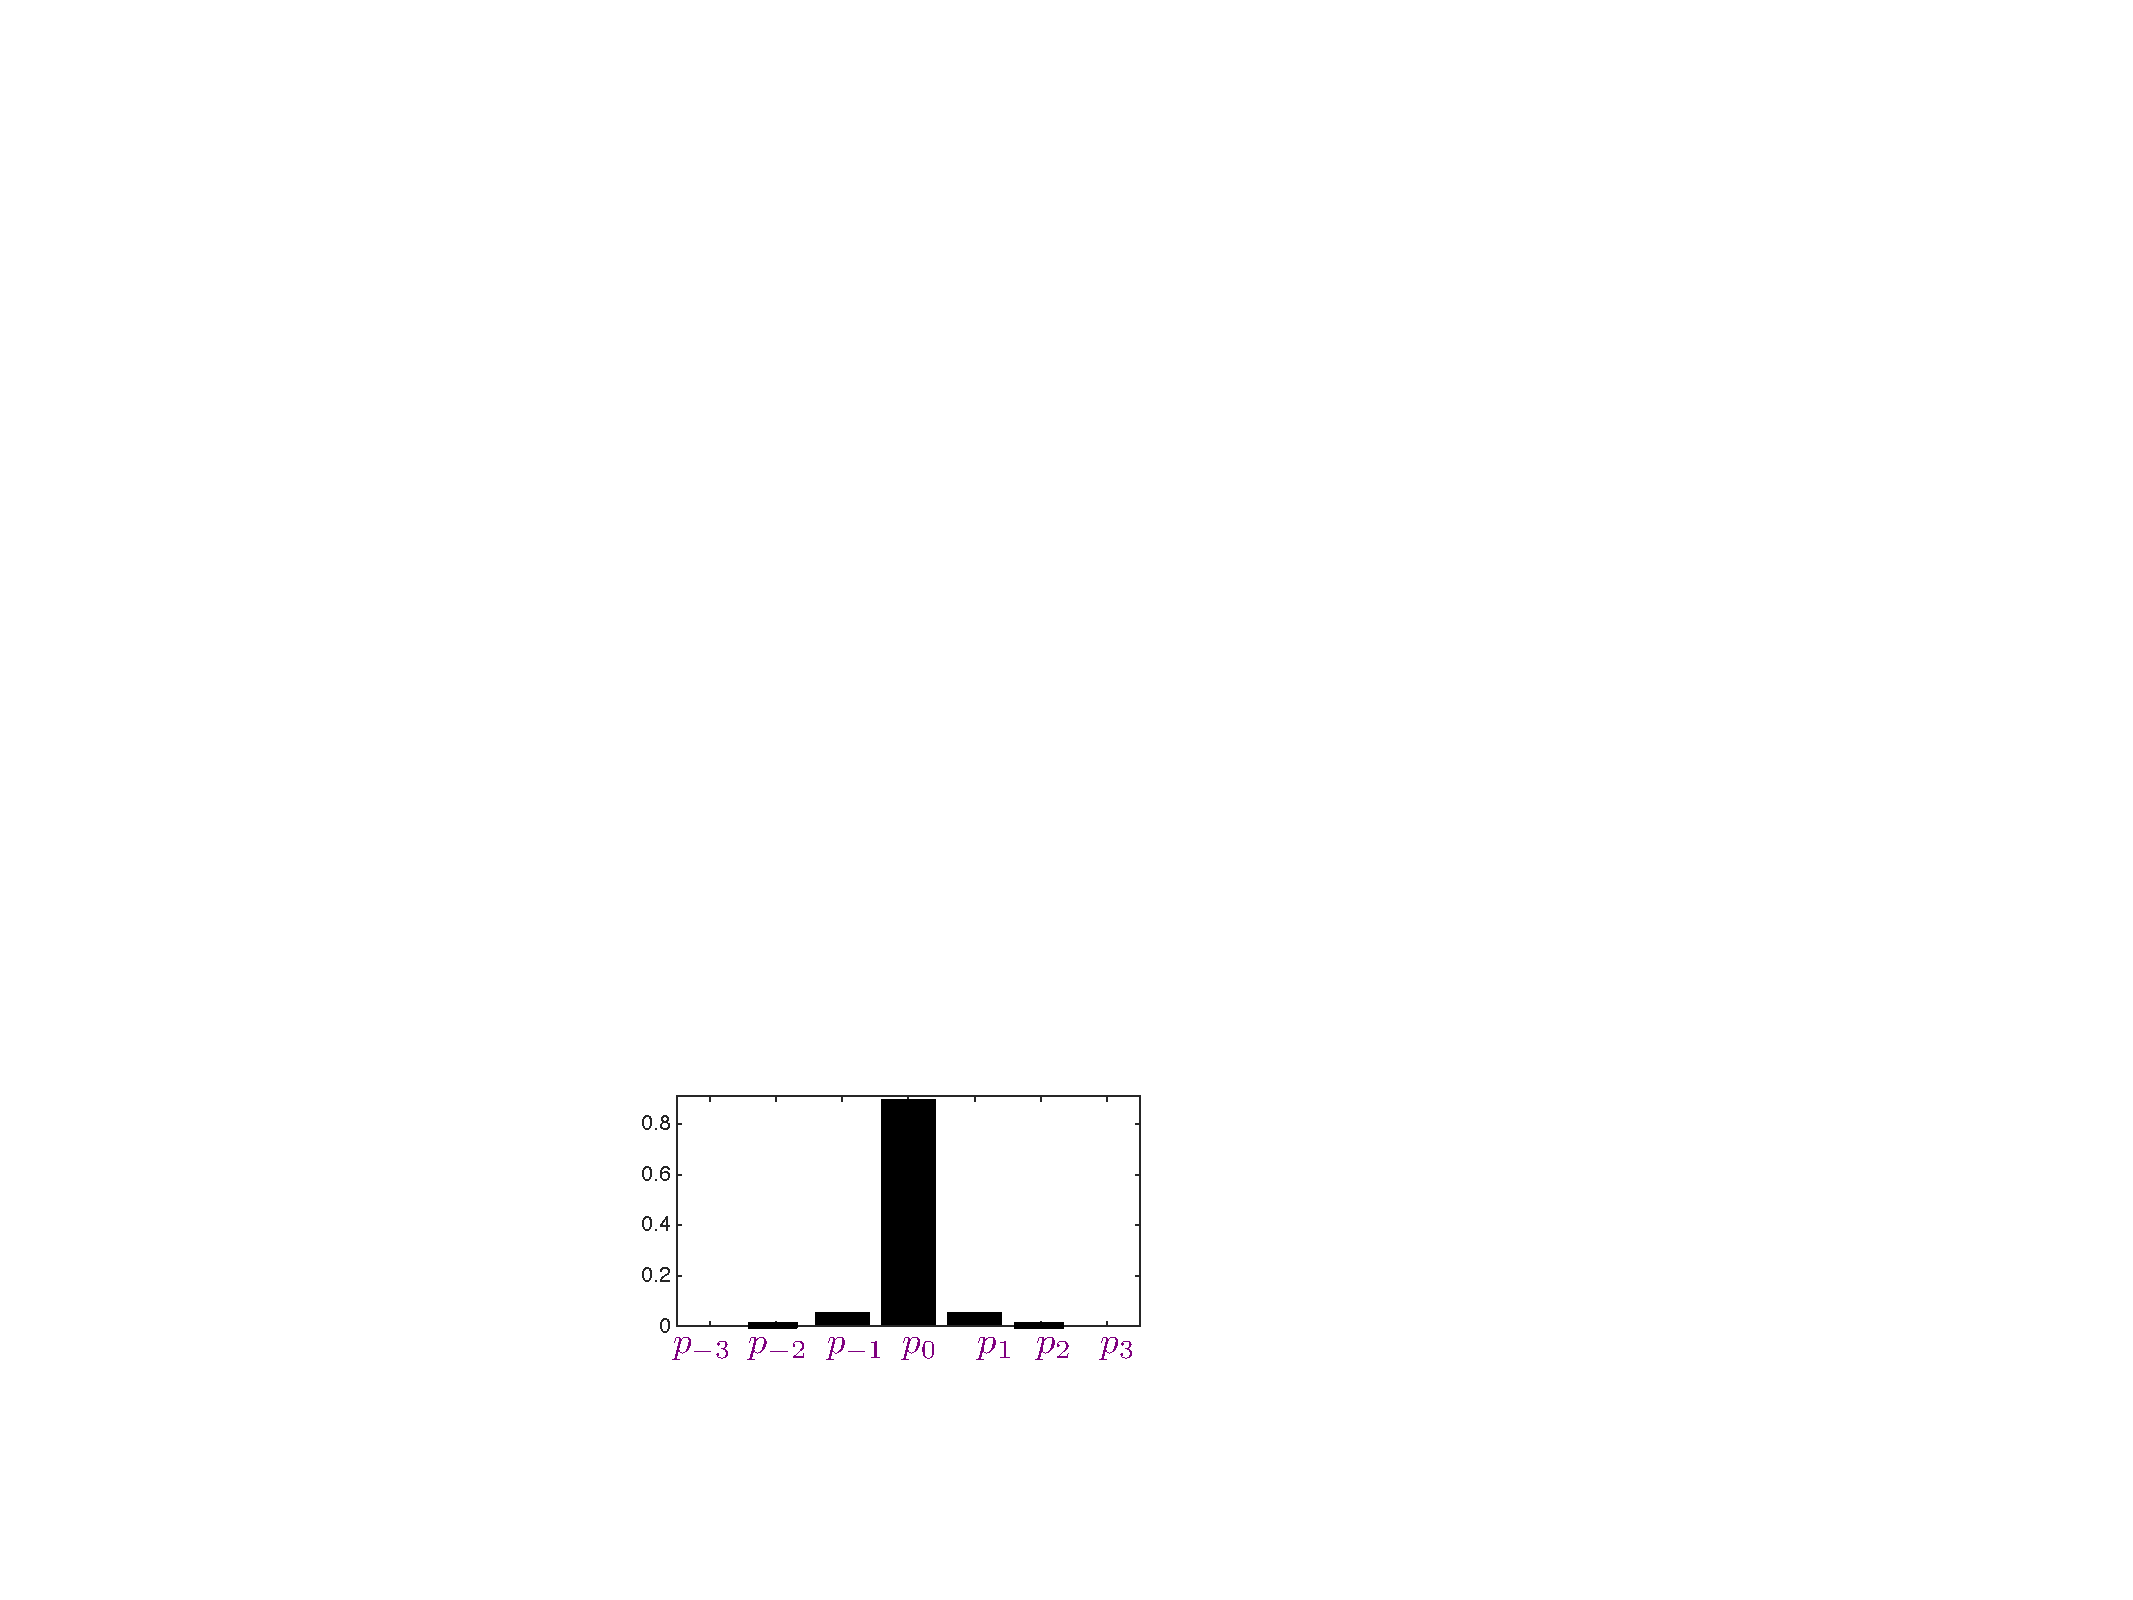
\includegraphics[width=.25\linewidth]{1-shannon/differences/histo-diff}&
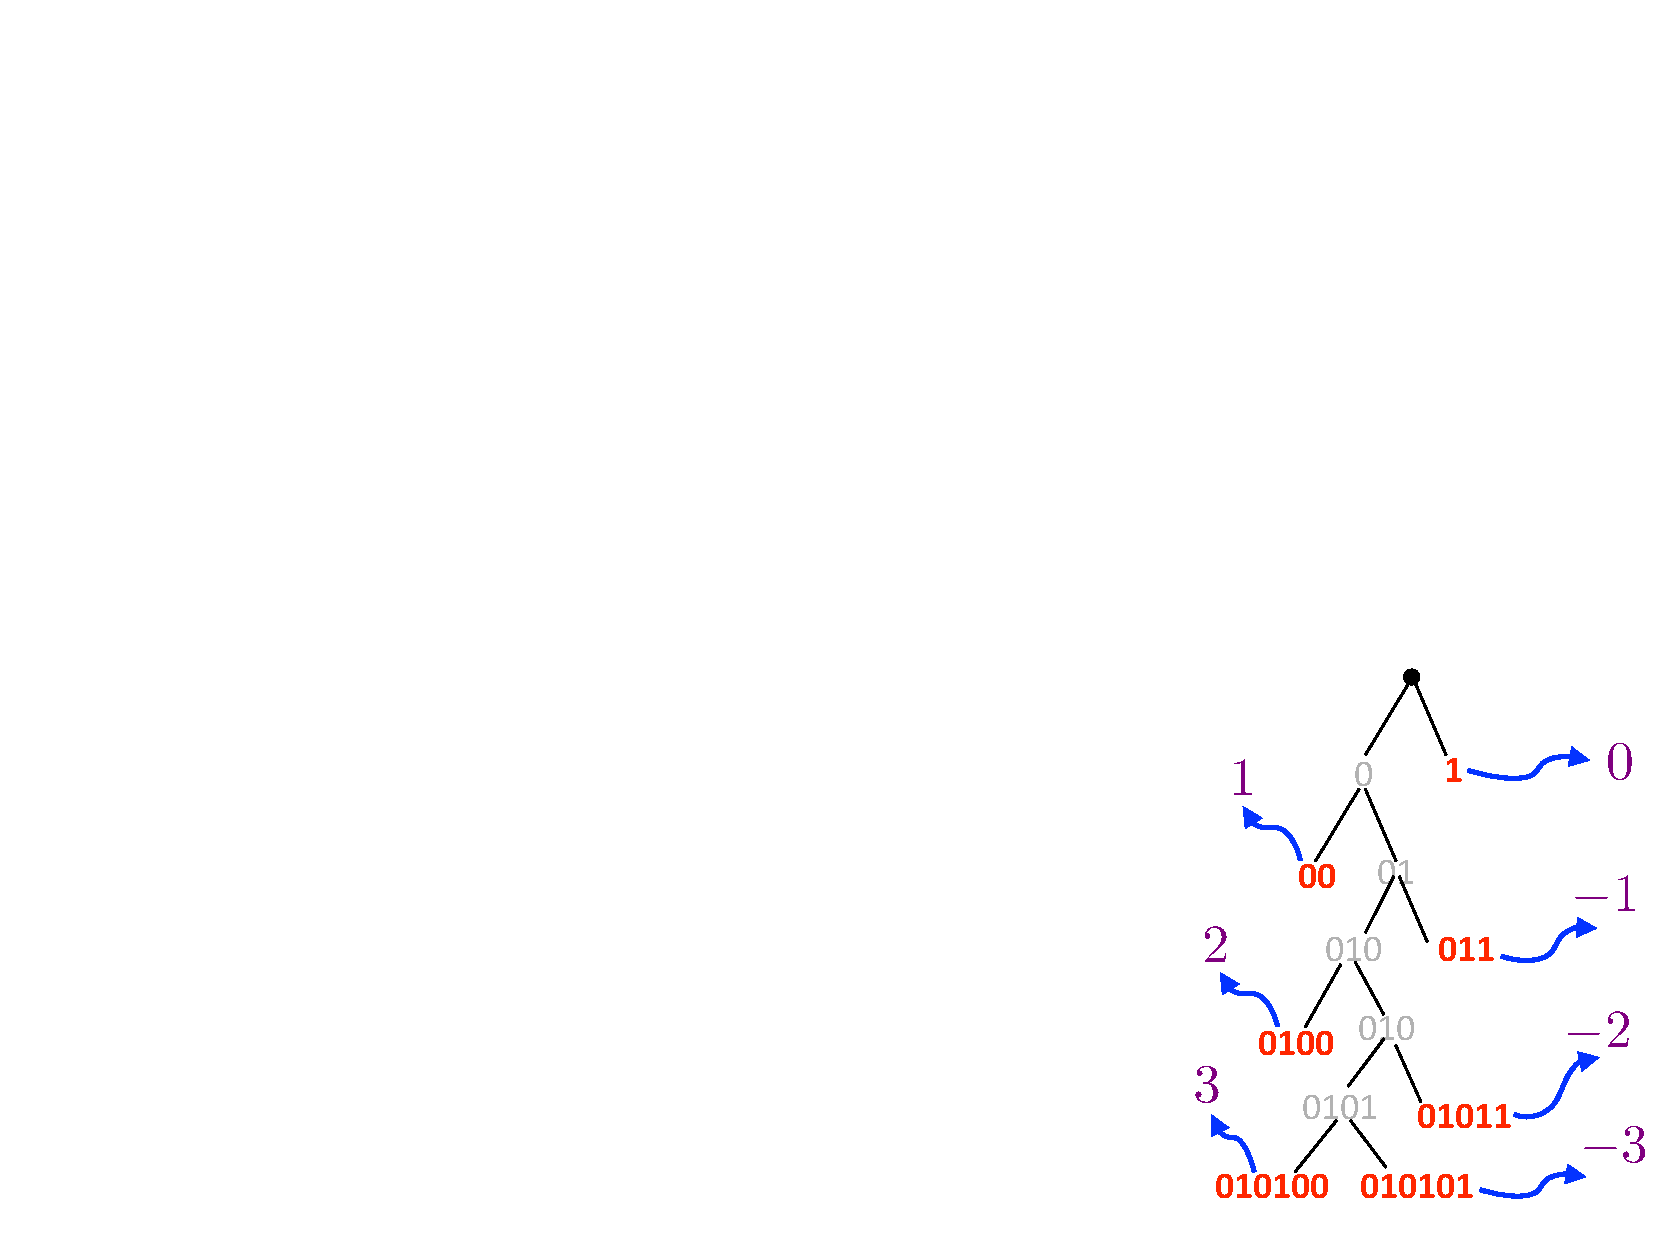
\includegraphics[width=.2\linewidth]{1-shannon/differences/arbre-difference}\\
$H(p) \approx 1.54, L(c) \approx 1.67 $ & $H(p) \approx 0.61, L(c) \approx 1.16 $ & Coding Tree
}
}{Top: retransformation by successive differences.
%
Bottom: comparison of histograms of pixel values and differences, and a code tree for these differences.
%
}{fig-codage-differences}

Another, more systematic way to leverage such temporal redundancy is by performing run-length-coding, which operate by grouping together sequence of similar symbols and thus coding first a symbol and then the length of the associated group (which is coded entropically). If the sequence is generated by a Markov chain, this method can be shown to asymptotically reach the Shannon bound where now the entropy is the entropy associated to the distribution of the Markov chain on infinite sequences (which can be computed as the limit of the entropy for finite sequences).




% !TEX root = ../FundationsDataScience.tex

\chapter{Fourier Transforms}
\label{sec-fourier}

The main references for this chapter is \cite{mallat2008wavelet}.
%
The Fourier transforms offers a perfect blend of analysis (solution of PDEs, approximation of functions), algebra (characters of groups, representation theory) and computer science (the FFT). 
%
It is the basics of signal processing because it allows to compute efficiently and study theoretically convolution operator, which are the shift-invariant operators. 
%
This chapter offers a glimpse of all these different facets. 

\newcommand{\piN}{\frac{2\imath\pi}{N}}

%%%%%%%%%%%%%%%%%%%%%%%%%%%%%%%%%%%%%%%%%%%%%%%%
%%%%%%%%%%%%%%%%%%%%%%%%%%%%%%%%%%%%%%%%%%%%%%%%
%%%%%%%%%%%%%%%%%%%%%%%%%%%%%%%%%%%%%%%%%%%%%%%%
\section{Hilbert spaces and Fourier Transforms}

%%%%%%%%%%%%%%%%%%%%%%%%%%%%%%%%%%%%%%%%%%%%%%%%
\subsection{Hilbertian bases.}

A large class of method in data sciences (including for instance most signal processing tasks, but also data pre-processing for machine learning) operate by first projecting the input data on some basis. A particularly simple instance of this is when the basis is orthogonal, since in this case one has a simple reconstruction formula and conservation of energy, which is crucial to do a theoretical analysis. We explain this in a general Hilbert space, which can be for instance $\Hh = L^2([0,1]^d)$ when dealing with continuous signal, or $\Hh=\RR^N$ for discrete signal.  

An (complex) Hilbert space $(\Hh,\dotp{\cdot}{\cdot})$ is complete, where $\dotp{\cdot}{\cdot}$ is an hermitian inner product (i.e. $\dotp{f}{g}$ is the conjugate of $\dotp{g}{f}$). If it is separable, it can be equipped with an Hilbertian orthogonal basis $(\phi_n)_{n \in \NN}$, which means that one can expand any $f \in \Hh$ as
\eq{
	f = \sum_{n} \dotp{f}{\phi_n} \phi_n 
}
where the convergence is in the sense of $\norm{f}^2 \eqdef \dotp{f}{f}$, i.e. $\norm{ f - \sum_{n=0}^N \dotp{f}{\phi_n} \phi_n } \rightarrow 0$ as $N \rightarrow +\infty$. One also have the conservation of energy 
\eq{
	\norm{f}^2 = \sum_n \dotp{f}{\phi_n}^2.
}

A way to construct such an ortho-basis is using Gram-Schmidt orthogonalization procedure. From some family $(\bar\phi_n)_n$, one defines $\phi_0=\bar\phi_0/\norm{\bar\phi_0}$, $\phi_n=\tilde\phi_n/\norm{\tilde\phi_n}$ where $\tilde\phi_n$ is computed as  $\tilde\phi_n=\bar\phi_n - \sum_{i<n} a_i \phi_i$, and by orthogonality $a_i = \dotp{\bar \phi_n}{\phi_i}$. 

On $L^2([-1,1])$ equipped with the usual inner product, orthogonalization of monomials defines the Legendre polynomials, so that
\eq{
	\phi_0(x)=1, \quad \phi_1(x)=x, \quad \phi_2(x) = \frac{1}{2}(3x^2-1), \quad \text{etc.}
}
On $L^2(\RR)$ equipped with a Gaussian measure $e^{x^2}\d x$, this leads to functions of the form $P_n(x) e^{-x^2}$ where $P_n$ are Hermite polynomials, $P_0(x)=1, P_1(x)=x, P_2(x)=x^2-1$. Intuitively, orthogonality forces $\phi_n$ to have $n$ ``oscillations'', e.g. orthogonal polynomials have exactly $n$ zeros.

Another example is provided by the Shannon interpolation theorem, which states that $( \sinc(x-n) )_n$ is an orthogonal basis of $\enscond{f}{\supp(\hat f) \subset [-\pi,\pi]}$ and the reconstruction formula is $f=\sum_n f(n) \sinc(x-n)$ so that $f_n = \dotp{f}{\sinc(x-n)}$. The convergence is in $L^2$ but it is actually also pointwise as shown in the proof of the previous chapter. 


Another way (that we do not detail here) to construct orthogonal bases is to consider the eigenvectors of some symmetric operator. We will show bellow that Fourier bases can be obtained this way, by considering translation-invariant operators (convolutions). 


%%%%%%%%%%%%%%%%%%%%%%%%%%%%%%%%%%%%%%%%%%%%%%%%
\subsection{Fourier basis on $\RR/2\pi\ZZ$.}

There is a flurry of different Fourier basis depending on the space on which it is defined. To get an orthogonal basis, it is important to consider compact spaces (otherwise one obtain a notion of Fourier transform, which is not a decomposition on a basis). 

On $L^2(\TT)$ where $\TT=\RR/2\pi\ZZ$, equipped with $\dotp{f}{g} \eqdef \frac{1}{2\pi}\int_\TT f(x) \bar g(x) \d x$, one can use the Fourier basis 
\eql{\label{eq-fourier-basis-1d}
	\phi_n(x) \eqdef e^{\imath n x}
	\qforq
	n \in \ZZ. 
}
One thus has
\eql{\label{eq-defn-fourier-coeffs}
	f = \sum_{n} \hat f_n e^{\imath n \cdot}
	\qwhereq
	\hat f_n \eqdef \frac{1}{2\pi}\int_0^{2\pi} f(x) e^{-\imath n x} \d x, 
}
in $L^2(\TT)$ sense. Pointwise convergence is delicate, see Section~\ref{subsec-sampling}.

Figure \ref{fig-fourier-wav}, left, shows examples of the real part of Fourier atoms.

\myfigure{
	\image{orthobases}{.4}{atoms-fourier}
	\image{orthobases}{.5}{atoms-wavelets}
}{%
	Left: 1D Fourier (real part), right: wavelet bases. %	
}{fig-fourier-wav}


We recall that for $f \in L^1(\RR)$, its Fourier transform is defined as
\eq{
	\foralls \om \in \RR, \quad
	\hat f(\om) \eqdef \int_\RR f(x) e^{-\imath x \om} \d x.
}
and this is extended to $L^2(\RR)$ by density. 

The connexion between the Fourier transform on $\RR$ and the Fourier coefficients on $\TT$ is given by the following diagram 
\eq{
	\begin{array}{rcccl}
						& f(x)  &  \overset{\Ff}{\longrightarrow} &  \hat f(\om) &\\
		\text{sampling}& \downarrow & & \downarrow &\text{periodization} \\
						& (f(n))_n  &  \overset{\text{Fourier serie}}{\longrightarrow} &  \sum_n f(n) e^{-\imath \om n} &\\
	\end{array}.
}
Its commutativity sates
\eql{\label{eq-poisson-bis}
	\sum_n f(n) e^{-\imath \om n} = \sum_n \hat f(\om-2\pi n)
}
and this is in fact the celebrated Poisson formula (Proposition~\ref{prop-poisson}). 



\myfigure{
\image{fourier}{.8}{fourier-transforms}
}{%
	The four different settings for Fourier analysis, and the sampling-periodization relationship.%	
}{fig-fourier-transforms}



%%%%%%%%%%%%%%%%%%%%%%%%%%%%%%%%%%%%%%%%%%%%%%%%
%%%%%%%%%%%%%%%%%%%%%%%%%%%%%%%%%%%%%%%%%%%%%%%%
%%%%%%%%%%%%%%%%%%%%%%%%%%%%%%%%%%%%%%%%%%%%%%%%
\section{Convolution on $\RR$ and $\TT$}

%%%%%%%%%%%%%%%%%%%%%%%%%%%%%%%%%%%%%%%%%%%%%%%%
\subsection{Convolution}

\wrapf{2-fourier/convolution}{Convolution on $\RR$.}
On $\XX=\RR$ or $\TT$, one defines 
\eql{\label{eq-convol-1d}
	f \star g(x) = \int_\XX f(t) g(x-t) \d t. 
}
Young's inequality shows that this quantity is well defined if $(f,g) \in L^p(\XX) \times L^q(\XX)$
\eql{\label{eq-young-convol}
	\frac{1}{p}+\frac{1}{q}=1+\frac{1}{r} \qarrq
	f \star g \in L^r(\XX) \qandq 
	\norm{f\star g}_{L^r(\XX)} \leq \norm{f}_{L^p(\XX)}\norm{g}_{L^q(\XX)}.
}
This shows that if $f \in L^1(\XX)$, then one has the map $g \in L^p(\XX) \mapsto f \star g \in L^p(\XX)$ is a continuous map on $L^p(\XX)$. Furthermore, when $r=\infty$, $f \star g \in \Cc^0(\XX)$ is a continuous function (which shows some regularizing effect).
%
Note that for $\XX=\TT$, $p<q \qarrq L^q(\TT) \subset L^p(\TT)$, so that $L^\infty(\XX)$ is the smallest space. 


\myfigure{
\image{fourier}{.6}{filtering-principle}
}{%
	Signal filtering with a box filter (running average). %	
}{fig-filter-box}

Convolution is mostly used in order to regularize functions. For instance, if $f \in L^1(\XX)$ and $g \in \Cc^1(\XX)$ is bounded, then $f \star g$ is differentiable and $(f \star g)'=f \star g'$. This is used to produce smooth approximate identity $(\rho_\epsilon = \frac{1}{\epsilon}\rho(\cdot/\epsilon))_\epsilon$ with convergence $f \star \rho_\epsilon \rightarrow f$ in $L^p(\XX)$ for $1 \leq p < +\infty$ of smooth approximations (and convergence in $L^\infty(\XX)$ if $f$ is uniformly continuous). 
%
This is also used for denoising applications in signal and image processing.


\myfigure{
\image{fourier}{.6}{filtering-1d-1}\\
\image{fourier}{.6}{filtering-1d-2}\\
\image{fourier}{.6}{filtering-1d-3}
}{%
	Filtering an irregular signal with a Gaussian filter of increasing filter size $\si$. %	
}{fig-filtering-1d}

%%% FIG %%%
\wrapf{2-fourier/convolution-fourier}{Commutative diagram of convolution-Fourier.}
%%%
For $(f,g) \in L^1(\XX)^2$ (so on $\XX=\TT$, also in any $L^p(\XX)$), one has
\eql{\label{eq-convol-fourier}
	\Ff(f \star g) = \hat f \odot \hat g
} 
which means that $\Ff$ is a morphism of algebra. For instance if $\XX=\RR$, its range is included in the algebra of continuous functions with vanishing limits in $\pm\infty$.

As shown in Figure~\ref{fig-splines}

\begin{figure}
\centering
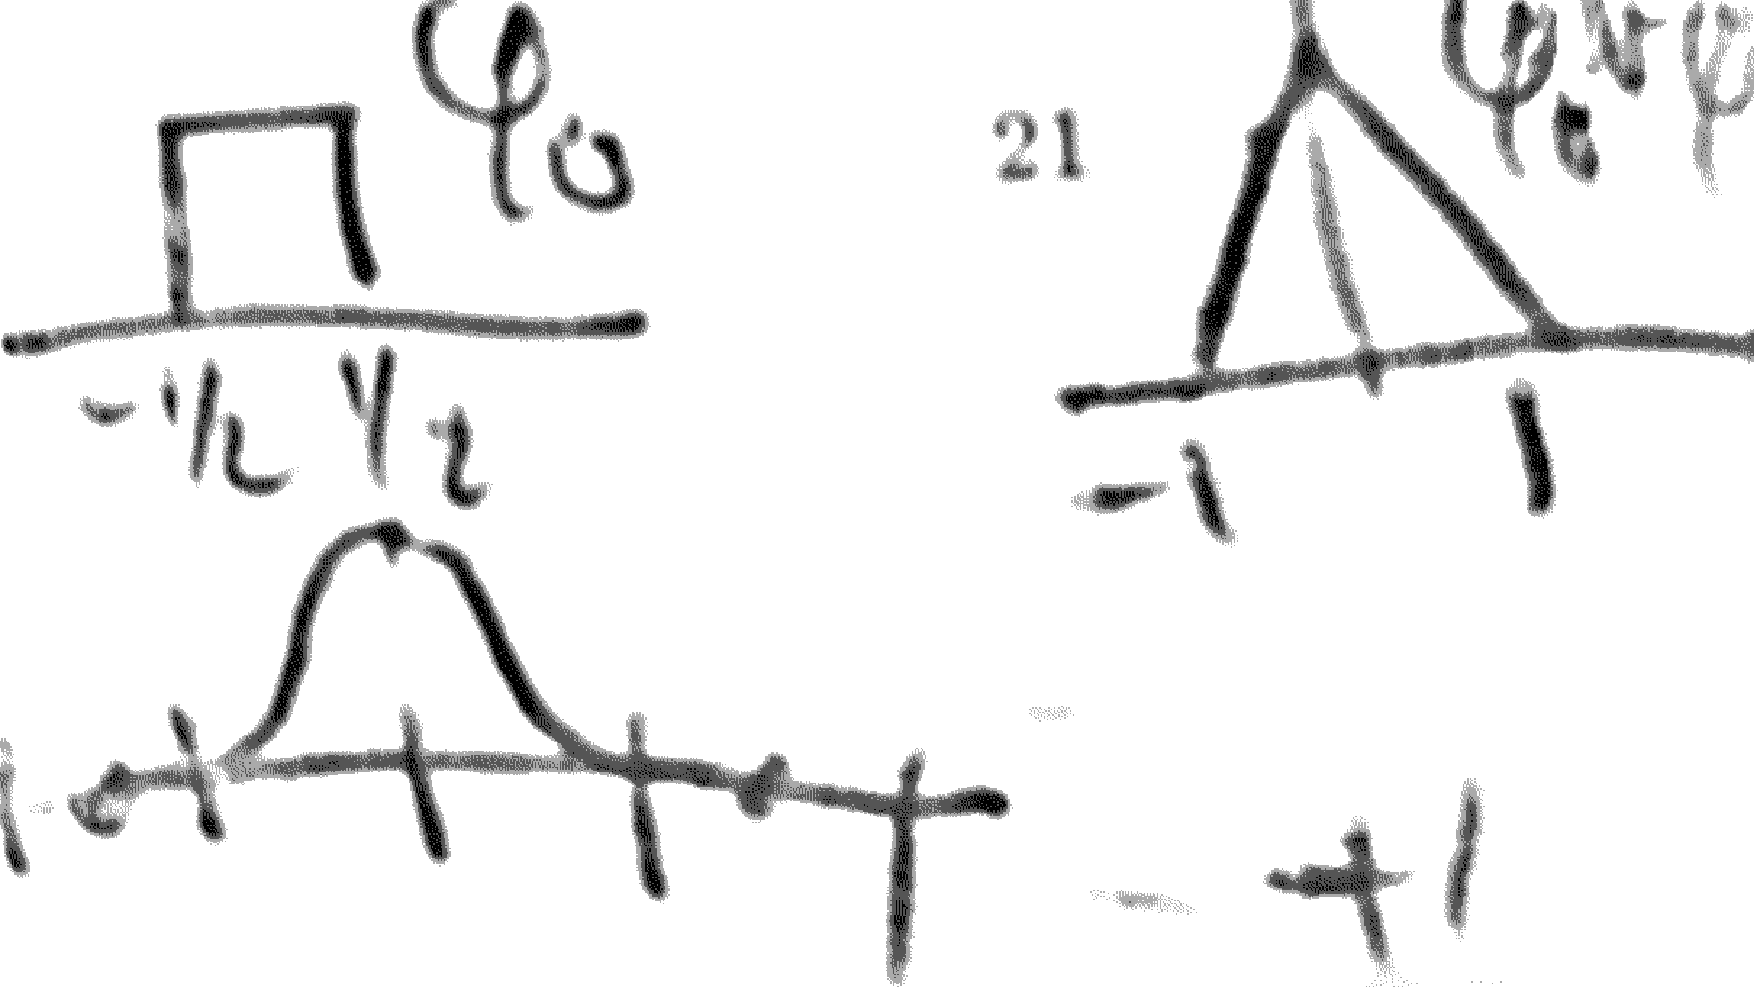
\includegraphics[width=.3\linewidth]{2-fourier/splines}
\caption{\label{fig-splines}
Cardinal splines are defined by successive convolutions;  
}
\end{figure}


Note also that the convolution is used extensively in probability and statistics, because if we denote $f_X$ the probability density (with respect to Lebesgue or any measure) of some random vector $X$, then if $X$ and $Y$ are independent random variable, then $f_{X+Y}=f_X \star f_Y$. 


\texttt{Associated code: fourier/test\_denoising.m and fourier/test\_fft2.m}

%%%%%%%%%%%%%%%%%%%%%%%%%%%%%%%%%%%%%%%%%%%%%%%%
\subsection{Translation Invariant Operators}

\wrapf{2-fourier/translation-inv}{Commutative diagram for translation invariance.}
Translation invariant operators (which commutes with translation) are fundamental because in most situations, input (signal, image, etc) should be processed without spatial preference.
%
The following propositions shows that any translation invariant\footnote{One should rather actually say ``translation equivariant''.} (i.e. which commutes with translations) operator is actually a ``convolution'' against a distribution with bounded Fourier transform. 
%
The proof and conclusion (regularity of the convolution kernel) vary depending on the topology on the input and output spaces.
%
We first study the case of convolution mapping to continuous functions.

\begin{prop}
	We define $T_\tau f = f(\cdot-\tau)$.
	%
 	A bounded linear operator $H : (L^2(\XX),\norm{\cdot}_2) \rightarrow (C^0(\XX),\norm{\cdot}_\infty)$ is such that for all $\tau$, $H \circ T_\tau = T_\tau \circ H$ if and only if 
	\eq{
		\foralls f \in L^2(\TT), \quad H(f) = f \star g
	}
	with $g \in L^2(\XX)$.
\end{prop}

The heuristic proof using distributions is that $f(x) = (f\star \de)(x) = \int f(t) \de(x-t) \d t$ and thus by linearity
\eq{
	Hf = H( \int f(t) \de(\cdot-t) \d t ) = \int f(t) H(\de(\cdot-t)) \d t
	=  \int f(t) H(T_t \de) \d t
	\int f(t) T_t(H(\de)) \d t
	\int f(t) H(\de)(\cdot -t) \d t
	= f \star H(\de).
}


\begin{proof}
	Thanks to~\eqref{eq-young-convol} (and the remark in the case $r=\infty$), $T : f \mapsto f \star g$ with $g \in L^2(\XX)$ is indeed a continuous operator from $L^2(\XX)$ to $C^0(\XX)$.  Furthermore
	\eq{
		(H \circ T_\tau)(f) = \int_\XX f( (\cdot-\tau)-y) g(y) \d \tau = (f \star g)(\cdot-\tau) = T_\tau (Hf), 
	}
	so that such an $H$ is translation-invariant. 
	
	
	Conversely, we define $\ell : f \mapsto H(f)(0) \in \RR$, which is legit since $H(f) \in \Cc^0(\XX)$. 
	%
	Since $H$ is continuous, there exists $C$ such that $\norm{Hf}_\infty \leq C \norm{f}_2$, and hence $|\ell(f)| \leq C \norm{f}_2$, so that $f$ is a continuous linear form on the Hilbert space $L^2(\XX)$. Hence, according to Fr\'echet-Riesz theorem, there exists $h \in L^2(\XX)$ such that $\ell(f)=\dotp{f}{h}$.
	%
	Hence, $\foralls x \in \XX$, 
	\eq{
		H(f)(x) = T_{-x} (Hf)(0) = H ( T_{-x} f)(0) = \ell( T_{-x} f ) = \dotp{T_{-x} f}{h} =
		\int_\XX f(y+x) h(y) \d y = f \star \bar h(x). 
	}
	where $g \eqdef \bar h=h(-\cdot) \in L^2(\XX)$.
\end{proof}

We now study, on $\TT$, the case of convolution which can output non-continuous functions. In this case, the kernel can be a ``distribution'', so the convolution is defined over the Fourier domain. 

\begin{prop}\label{prop-ti-convol-l2}
 	A bounded linear operator $H : L^2(\TT) \rightarrow L^2(\TT)$ is such that for all $\tau$, $H \circ T_\tau = T_\tau \circ H$ if and only if 
	\eq{
		\foralls f \in L^2(\TT), \quad
		\Ff( H(f) ) = \hat f \odot c 
	}
	where $c \in \ell^\infty(\ZZ)$ (a bounded sequence).
\end{prop}
\begin{proof}
	We denote $\phi_n \eqdef e^{\imath n \cdot}$. 
	One has
	\eq{
		H(\phi_n) = e^{\imath n \tau} H(T_\tau(\phi_n)) = e^{\imath n \tau} T_\tau(H(\phi_n)).
	}
	Thus, for all $n$, 
	\eq{
		\dotp{H(\phi_n)}{\phi_m} 
		= e^{\imath n \tau} \dotp{T_\tau \circ H(\phi_n)}{\phi_m} 
		= e^{\imath n \tau} \dotp{H(\phi_n)}{ T_{-\tau}(\phi_m) }
		=  e^{\imath (n-m) \tau} \dotp{H(\phi_n)}{ \phi_m }
	}
	So for $n \neq m$, $\dotp{H(\phi_n)}{\phi_m} = 0$, and we define $c_n \eqdef \dotp{H(\phi_n)}{\phi_n}$. Since $H$ is continuous, $\norm{Hf}_{L^2(\TT)} \leq C \norm{f}_{L^2(\TT)}$ for some constant $C$, and thus
	by Cauchy-Schwartz 
	\eq{
		|c_n| = |\dotp{H(\phi_n)}{\phi_n}| \leq \norm{H(\phi_n)} \norm{\phi_n} \leq C 
	}	
	because $\norm{\phi_n}=1$, so that $c \in \ell^\infty(\ZZ)$.
	%
	By continuity, recalling that by definition $\hat f_n \eqdef \dotp{f}{\phi_n}$, 
	\eq{
		H(f) = \lim_N H( \sum_{n=-N}^N \hat f_n \phi_n ) = \lim_N \sum_{n=-N}^N \hat f_n H(\phi_n)
		= \lim_N \sum_{n=-N}^N c_n \hat f_n \phi_n = \sum_{n \in \ZZ} c_n \hat f_n \phi_n
	} 
	so that in particular one has the desired result.
\end{proof}

This theorem thus states that translation invariant operators are those which are ``diagonal'' in the Fourier ortho-basis. 

%%%%%%%%%%%%%%%%%%%%%%%%%%%%%%%%%%%%%%%%%%%%%%%%
\subsection{Revisiting Poisson formula using distributions.}

Informally, the Fourier series
\eq{
	\sum_n f(n) e^{-\imath \om n}
} 
can be thought as the Fourier transform $\Ff( \Pi_1 \odot f )$ of the discrete distribution
\eq{
	\Pi_1 \odot f = \sum_n f(n) \de_{n}
	\qwhereq
	\Pi_s = \sum_n \de_{sn}
}
for $s \in \RR$, 
where $\de_a$ is the Dirac mass at location $a \in \RR$, i.e. the distribution such that $\int f \d(\d_a)=f(a)$ for any continuous $f$. Indeed, one can multiply a distribution by a continuous function, and the definition of the Fourier transform of a distribution $\mu$ is a distributions $\Ff(\mu)$ such that that 
\eq{
	\foralls g \in \Ss(\RR), \quad \int_\RR g(x) \d \Ff(\mu) = \int_\RR \Ff^*(g) \d \mu, 
	\qwhereq
	\Ff^*(g) \eqdef \int_\RR g(x) e^{\imath x \cdot} \d x, 
}
where $\Ss(\RR)$ are smooth and rapidly decaying (Schwartz class) functions.

\wrapf{2-fourier/poisson-distrib}{Sine wave being summed in the Poisson formula.}
The Poisson formula~\eqref{eq-poisson-bis} can thus be interpreted as
\eq{
	\Ff(\Pi_1 \odot f) = \sum_n \hat f(\cdot-2\pi n) = \int_\RR \hat f(\cdot-\om) \d\Pi_{2\pi}(\om)  = \hat f \star \Pi_{2\pi}
}
Since $\Ff^{-1} = \frac{1}{2\pi} \Ss \circ \Ff$ where $\Ss(f)=f(-\cdot)$, one has, applying this operator on both sides
\eq{
	\Pi_1 \odot f = \frac{1}{2\pi} \Ss \circ \Ff(\hat f \star \Pi_{2\pi}) =  \Ss(  \frac{1}{2\pi} \Ff(\hat f) \odot \hat\Pi_{2\pi})
	= \Ss(  \frac{1}{2\pi} \Ff(\hat f) ) \odot \Ss(\hat\Pi_{2\pi}) = \hat \Pi_{2\pi} \odot f.
}
This can be interpreted as the relation
\eq{
	\hat\Pi_{2\pi} = \Pi_{1}
	\qarrq
	\hat\Pi_1 = 2\pi \Pi_{2\pi}.
}

To intuitively understand this relation, one can compute a finite Fourier series
\eq{
	\sum_{n=-N}^N e^{-\imath n \om} = \frac{ \sin( (N+1/2) x) }{\sin(x/2)}
}
which is a smooth function which grows unbounded with $N \rightarrow +\infty$ as $N \rightarrow +\infty$. 

%%%%%%%%%%%%%%%%%%%%%%%%%%%%%%%%%%%%%%%%%%%%%%%%
%%%%%%%%%%%%%%%%%%%%%%%%%%%%%%%%%%%%%%%%%%%%%%%%
%%%%%%%%%%%%%%%%%%%%%%%%%%%%%%%%%%%%%%%%%%%%%%%%
\section{Finite Fourier Transform and Convolution}
\label{sec-dft}

%%%%%%%%%%%%%%%%%%%%%%%%%%%%%%%%%%%%%%%%%%%
\subsection{Discrete Ortho-bases}

Discrete signals are finite dimensional vector $f \in \CC^N$ where $N$ is the number of samples and where each $f_n$ is the value of the signal at a 1D or 2D location. For a 2-D images $f \in \CC^N \simeq \CC^{N_0 \times N_0}$, $N = N_0 \times N_0$, where $N_0$ is the number of pixels along each direction.

Discrete signals and images are processed using a discrete inner product that mimics the continuous $\Ldeux$ inner product
\eq{
	\dotp{f}{g} = \sum_{n=0}^{N-1} f_n \bar g_n.
}
One thus defines a distance between discretized vectors as
\eq{
	\norm{f-g}^2 = \sum_{n=0}^{N-1} |f_n-g_n|^2.
}

Exactly as in the continuous case, a discrete orthogonal basis $\{ \psi_m \}_{0 \leq m < N }$ of $\CC^N$, satisfies
\eql{\label{eq-orthobasis-disc}
	\dotp{\psi_m}{\psi_{m'}} = \de_{m-m'}.
}
The decomposition of a signal in such an ortho-basis is written
\eq{
	f = \sum_{m=0}^{N-1} \dotp{f}{\psi_m} \psi_m.
}
It satisfies a conservation of energy
\eq{
	\norm{f}^2 = \sum_{n=0}^{N-1} |f_n|^2 = 
\sum_{m=0}^{N-1} |\dotp{f}{\psi_m}|^2
}

Computing the set of all inner product $\{\dotp{f}{\psi_m}\}_{0 \leq m < N}$ is done in a brute force way in $O(N^2)$ operations.
This is not feasible for large datasets where $N$ is of the order of millions. When designing an ortho-basis, one should keep this limitation in mind and enforce some structure in the basis elements so that the decomposition can be computed with fast algorithm. This is the case for the Fourier and wavelet bases, that enjoy respectively $O(N\log(N))$ and $O(N)$ algorithms.


%%%%%%%%%%%%%%%%%%%%%%%%%%%%%%%%%%%%%%%%%%%%%%%%
\subsection{Discrete Fourier transform}

We denote $f = (f_n)_{n=0}^{N-1} \in \RR^N$, but we insists that such vector should really be understood as being indexed by $n \in \ZZ/N\ZZ$, which is a finite commutative group for the addition. This corresponds to using periodic boundary conditions. 

The discrete Fourier transform is defined as
\eql{\label{eq-dft}
	\foralls k=0,\ldots,N-1, \quad \hat f_k \eqdef \sum_{n=0}^{N-1} f_n e^{-\piN kn} = \dotp{f}{\phi_k}
	\qwhereq
	\phi_k \eqdef ( e^{\piN kn} )_{n=0}^{N-1} \in \CC^N
}
where the canonical inner product on $\CC^N$ is $\dotp{u}{v}=\sum_{n=1}^N u_n \bar v_n$ for $(u,v) \in (\CC^N)^2$.
%
This definition can intuitively be motivated by sampling the Fourier basis $x \mapsto e^{\imath k x}$ on $\RR/2\pi\ZZ$ at equi-spaced points $( \frac{2\pi}{N}n )_{n=0}^{N-1}$.
%
The following proposition shows that this corresponds to a decomposition in an ortho-basis.

\begin{prop}
	One has
	\eq{
		\dotp{\phi_k}{\phi_\ell} = \choice{
			N \qifq k=\ell, \\
			0 \quad\text{otherwise.}
		}
	}
	In particular, this implies
	\eql{\label{eq-dft-inv}
		\foralls n=0,\ldots,N-1, \quad
		f_n = \frac{1}{N}\sum_k \hat f_k e^{\piN kn}. 
	}
\end{prop}
\begin{proof}
	One has, if $k \neq \ell$
	\eq{
		\dotp{\phi_k}{\phi_\ell} = \sum_n e^{\piN (k-\ell) n} = 
		\frac{ 1 - e^{\piN (k-\ell) N} }{ 1 - e^{\piN (k-\ell)} } = 0
	}
	which is the sum of a geometric serie (equivalently, sum of equi-spaced points on a circle). 
	%
	The inversion formula is simply $f = \sum_k \dotp{f}{\phi_k} \frac{\phi_k}{\norm{\phi_k}^2}$.
\end{proof}


%%%%%%%%%%%%%%%%%%%%%%%%%%%%%%%%%%%%%%%%%%%%%%%%
\subsection{Fast Fourier transform}

Assuming $N=2N'$, one has 
\begin{align*}
	\hat f_{2k} &= \sum_{n=0}^{N'-1} (f_n + f_{n+N/2}) e^{ -\frac{2\imath\pi}{N'} k n } \\
	\hat f_{2k+1} &= \sum_{n=0}^{N'-1} e^{ -\frac{2\imath\pi}{N'} n } (f_n - f_{n+N/2}) e^{ -\frac{2\imath\pi}{N'} k n }.
\end{align*}
For the second line, we used the computation
\eq{
	e^{-\frac{2\imath\pi}{N}(2k+1)(n+N/2)} =
	e^{-\frac{2\imath\pi}{N}(2kn+kN+n+N/2)} = - e^{ -\frac{2\imath\pi}{N'} n } e^{ -\frac{2\imath\pi}{N'} k n }.
}
Denoting $\Ff_N(f)=\hat f$ the discrete Fourier transform on $\RR^N$, and 
introducing the notation $f_e = (f_n + f_{n+N/2})_n \in \RR^{N'}$, $f_o = (f_n - f_{n+N/2})_n \in \RR^{N'}$
and $\al_N = (  e^{ -\frac{2\imath\pi}{N'} n } )_{n} \in \RR^{N'}$, one has the following recursion formula
\eq{
	\Ff_N(f) = \Ii_N( \Ff_{N/2}(f_e), \Ff_{N/2}(f_o \odot \al_N) )
}
where $\Ii_N$ is the ``interleaving'' operator, defined by $\Ii_N(a,b) \eqdef (a_1,b_1,a_2,b_2,\ldots,a_{N'},b_{N'})$.
%
There iterations define the so-called Fast Fourier Transform algorithm, which works here when $N$ is a power of 2. These iterations can be extended to arbitrary number $N$, but a workaround is to simply pad with 0 (or use more complicated extensions) to have vector with size that are power of $2$. 

This algorithm can also be interpreted as a factorization of the Fourier matrix into $O(\log(N))$ product of matrices. 

\begin{figure}
\centering
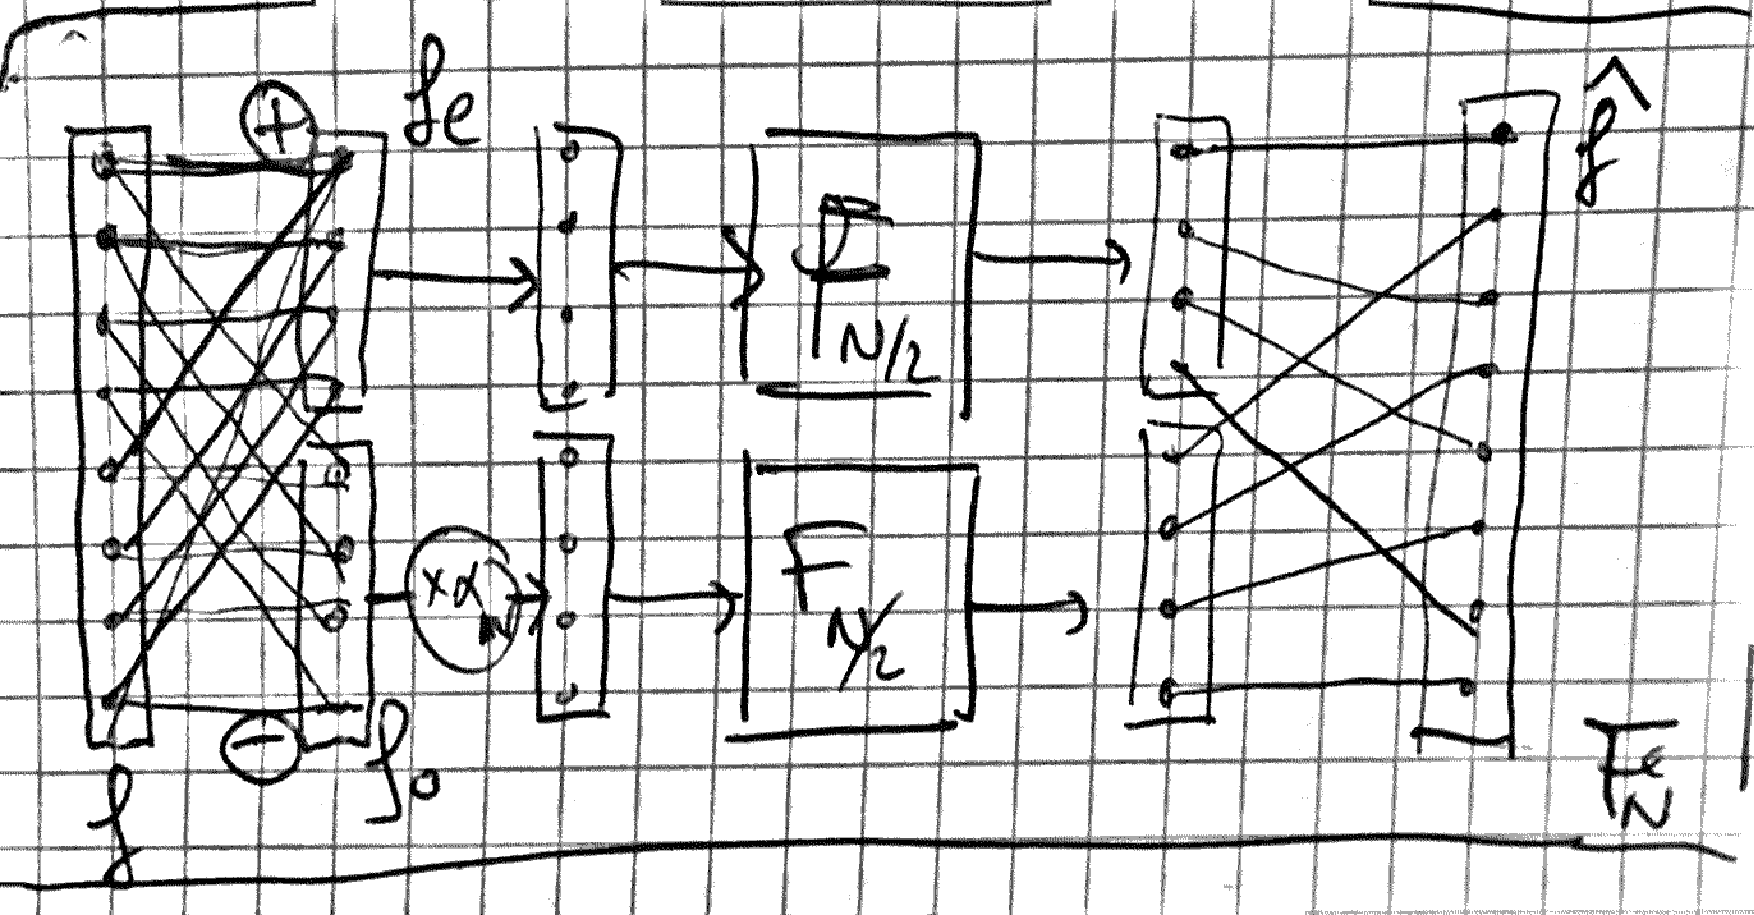
\includegraphics[width=.5\linewidth]{2-fourier/fft}
\caption{\label{fig-fft}
Diagram of one step of the FFT.
}
\end{figure}
 

Denoting $C(N)$ the numerical complexity (number of elementary operations) associated to the computation of $\hat f$, one thus has
\eql{\label{eq-cplx-fft}
	C(N) = 2C(N/2)+NK
}
where $K N$ is the complexity of $N$ complex additions and $N/2$ multiplications. Making the change of variable 
\eq{
	\ell \eqdef \log_2(N)
	\qandq 
	T(\ell) \eqdef \frac{C(N)}{N}
}
i.e. $C(N)=2^\ell T(\ell)$, the relation~\eqref{eq-cplx-fft} becomes
\eq{
	2^\ell T(\ell) = 2 \times 2^{\ell-1} T(\ell-1) + 2^\ell K \qarrq
	T(\ell) = T(\ell-1) + K \qarrq
	T(\ell) = T(0) + K \ell
} 
and using the fact that $T(0)=C(1)/1=0$, one obtains
\eq{
	C(N) = K N \log_2(N).
}
This complexity should be contrasted with the complexity $O(N^2)$ of directly computing the $N$ coefficients~\eqref{eq-dft}, each involving a sum of size $N$. 


%%%%%%%%%%%%%%%%%%%%%%%%%%%%%%%%%%%%%%%%%%%%%%%%
\subsection{Finite convolution}

For $(f,g) \in (\RR^{N})^2$, one defines $f\star g \in \RR^N$ as
\eql{\label{eq-finite-convol}
	\foralls n=0,\ldots,N-1, \quad
	(f \star g)_n \eqdef \sum_{k=0}^{N-1} f_k g_{n-k} = \sum_{k+\ell=n} f_k g_\ell 
}
where one should be careful that here $+$ and $-$ should be understood modulo $N$ (vectors should be seen as being defined on the group $\ZZ/N\ZZ$, or equivalently, one uses periodic boundary conditions).
%
This defines an commutative algebra structure $(\RR^N,+,\star)$, with neutral element the ``Dirac'' $\de_0 \eqdef (1,0,\ldots,0)^\top \in \RR^N$. The following proposition shows that $\Ff : f \mapsto \hat f$ is an algebra bijective isometry (up to a scaling by $\sqrt{N}$ of the norm) mapping to $(\RR^N,+,\odot)$ with neutral element $\ones_N=(1,\ldots,1) \in \RR^N$.

\begin{prop}\label{prop-tfd-conv}
	One has $\Ff( f \star g ) = \hat f \odot \hat g$. 
\end{prop}
\begin{proof}
	We denote $T : g \mapsto f \star g$. One has 
	\eq{
		(T \phi_\ell)_n = \sum_k f_k e^{ \piN \ell(n-k) } = e^{ \piN \ell n } \hat f_\ell.
	}
	This shows that $(\phi_\ell)_\ell$ are the $N$ eigenvectors of $T$ with associated eigenvalues $\hat f_\ell$. So $T$ is diagonalizable in this basis. Denoting $F=(  e^{ -\piN k n } )_{k,n}$ the matrix of the Fourier transform, the Fourier inversion formula~\eqref{eq-dft-inv} reads $F^{-1} = \frac{1}{N}F^*$ where $F^*=\bar F^\top$ is the adjoint matrix (trans-conjugate). The diagonalization of $T$ now reads
	\eq{
		T = F^{-1} \diag(\hat f) F =  \qarrq
		\Ff(T g) = \diag(\hat f) F g \qarrq
		\Ff(f \star g) = \diag(\hat f) \hat g.
	} 
\end{proof}

This proposition shows that one can compute in $O(N\log(N))$ operation via the formula
\eq{	
	f \star g = \FF^{-1}( \hat f \odot \hat g ).
}
This is very advantageous with respect to the naive implementation of formula~\eqref{eq-finite-convol}, in the case where $f$ and $g$ have large support. In case where $|\Supp(g)|=P$ is small, then direct implementation is $O(PN)$ which might be advantageous. An example is $g=[1,1,0,\ldots,0,1]/3$, the moving average, where
\eq{
	(f \star g)_n = \frac{f_{n-1}+f_n+f_{n+1}}{3}
}
needs $3N$ operations.

WARNING: this is wrong, one needs also to carie reminders in the multiplication. 
An example of application of the FFT is the multiplication of large polynomial, and thus of large integers (viewing the expansion in a certain basis as a polynomial). Indeed
\eq{
	(\sum_{i=0}^A a_i X_i)( \sum_{j=0}^B b_i X^j ) = 
	\sum_{k=0}^{A+B} ( \sum_{i+j=k} a_i b_j ) X^k
}
One can write $\sum_{i+j=k} a_i b_j = (\bar a \star \bar b)_k$ when one defines $\bar a,\bar b \in \RR^{A+B}$ by zero padding. 


%%%%%%%%%%%%%%%%%%%%%%%%%%%%%%%%%%%%%%%%%%%%%%%%
%%%%%%%%%%%%%%%%%%%%%%%%%%%%%%%%%%%%%%%%%%%%%%%%
%%%%%%%%%%%%%%%%%%%%%%%%%%%%%%%%%%%%%%%%%%%%%%%%
\section{Discretisation Issues}
\label{sec-fourier-discretization}

Beside computing convolutions, another major application of the FFT is to approximate the Fourier transform and its inverse, thus leading to a computationally efficient spectral interpolation method.


%%%%%%%%%%%%%%%%%%%%%%%%%%%%%%%%%%%%%%%%%%%%%%%%
\subsection{Fourier approximation via spatial zero padding.}

It is possible to view the discrete finite Fourier transform~\eqref{eq-dft} as a first order approximation to compute Fourier coefficients, or rather actually samples from the Fourier transform~\eqref{eq-fourier-transform}. Supposing that $f$ is a smooth enough function is supported on $[0,1]$, we consider the discrete Fourier transform of the vector $f^Q \eqdef (f(n/N))_{n=0}^{Q-1} \in \RR^Q$  where $Q \geq N$ induced a padding by $0$ (since $f(n/N)=0$ for $n > N$)
\eq{
	\foralls k \in \range{-\frac{Q}{2},\frac{Q}{2}}, \quad
	\frac{1}{N} \hat f_k^Q = \frac{1}{N} \sum_{n=0}^{N-1} f\pa{\frac{n}{N}} e^{-\frac{2\imath\pi}{Q} n k}
	\approx \int_0^1 f(x) e^{-\frac{2 k\imath\pi}{T} x} \d x = \hat f\pa{\frac{2 k \pi}{T}}
	\qwhereq
	T \eqdef \frac{Q}{N}.
}
The approximation is first order accurate, i.e. $O(1/N)$ for a $C^1$ function $f$. 
% FAUX Increasing the amount $Q$ of zero padding is a way to compute larger frequencies. Increasing the discretization precision $N$ is on contrary a way to increase the precision of the Fourier sampling (using smaller step size $2\pi/T$). 

\begin{figure}
\centering
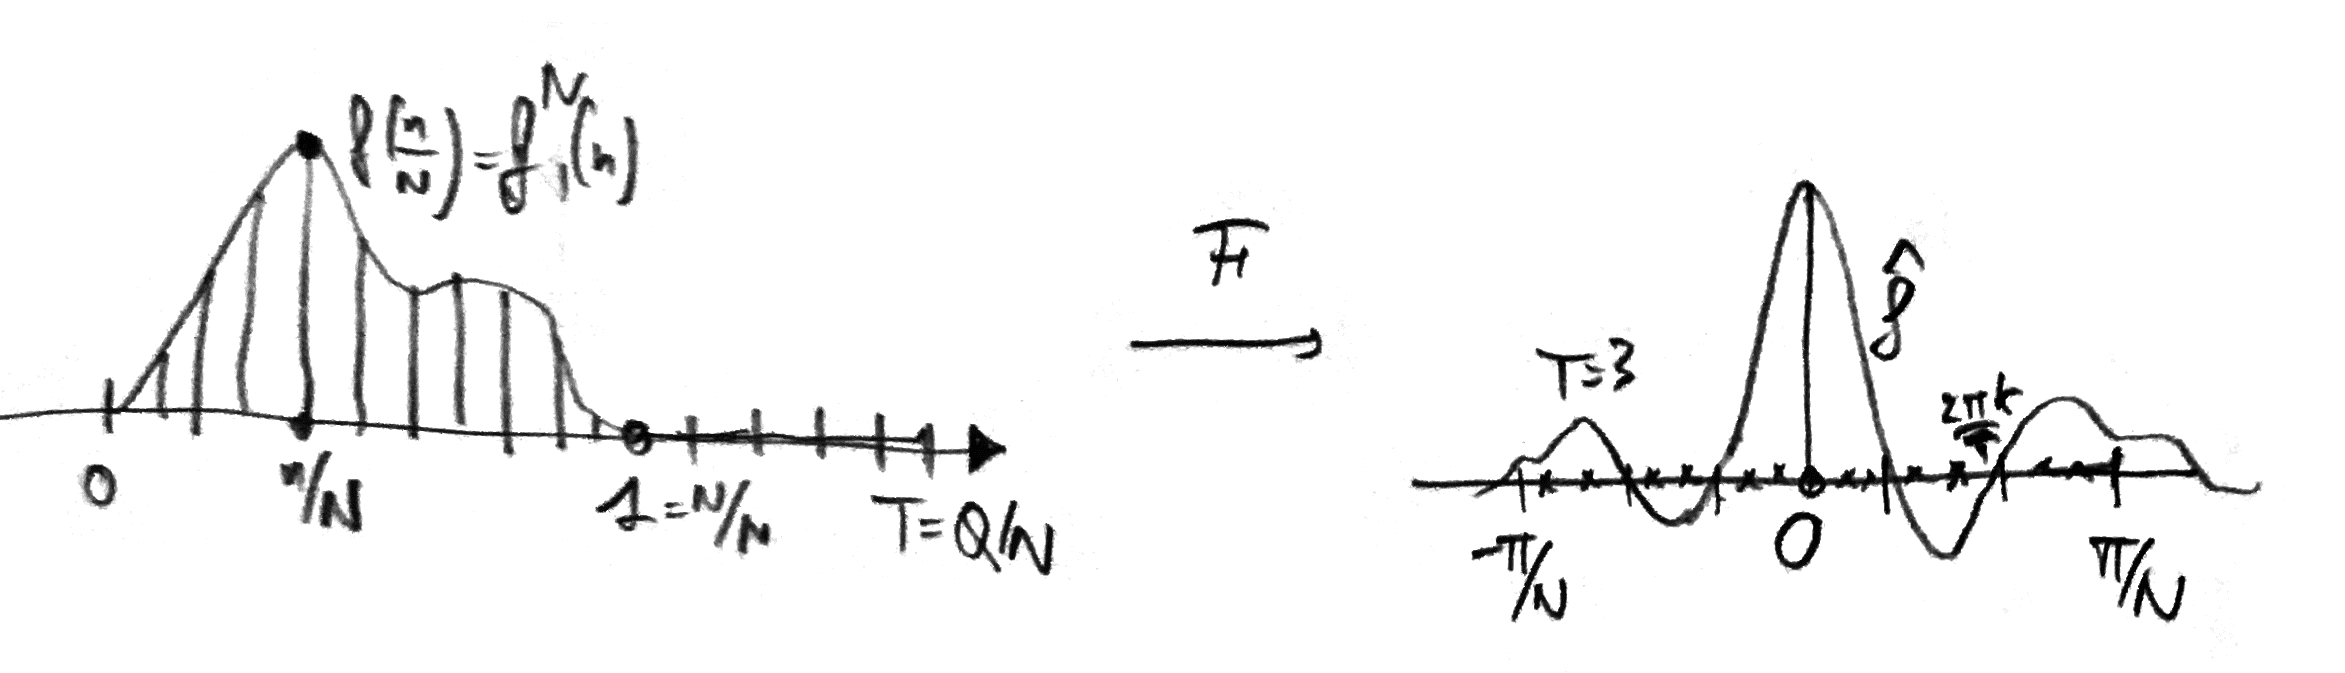
\includegraphics[width=.75\linewidth]{2-fourier/padding-spacial}
\caption{\label{fig-padding-spacial}
Fourier transform approximation by zero-padding in the spatial domain.
}
\end{figure}


%%%%%%%%%%%%%%%%%%%%%%%%%%%%%%%%%%%%%%%%%%%%%%%%
\subsection{Fourier interpolation via spectral zero padding.}

One can reverse the roles of space and frequency in the previous construction. 
%
If one has at its disposal $N$ uniform discrete samples $f^N=(f^N_n)_{n=0}^{N-1}$, one can compute its discrete Fourier transform $\Ff(f^N) = \hat f^N$ (in $O(N \log(N))$ operations with the FFT), 
\eq{
	\hat f^N_k \eqdef \sum_{n=0}^{N-1} f^N_n e^{-\frac{2\imath\pi}{N} n k}, 
}
and then zero-pad it to obtain a vector of length $Q$.
%
For simplicity, we assume $N=2N'+1$ is odd, and this computation can be also done (but is more involved) with even size.
%
Indexing the frequencies as $-N' \leq k \leq N'$ The padding vector is of the form, 
\eq{
	\tilde f^Q \eqdef (0,\ldots,0,\hat f^N,0,\ldots,0) \in \RR^Q
} 

WARNING: there is most likely an error in the following derivation, should be rewritten.
One can then compute the (with a normalization constant $Q/N$) inverse discrete Fourier transform of size $Q$ (in $O(Q \log(Q))$ operations with the FFT) to obtain
\begin{align*}
	\frac{Q}{N} \Ff^{-1}( \tilde f^Q )_\ell &= 
	\frac{Q}{N} \times \frac{1}{N} \sum_{k=-N'}^{N'} \hat f_k^N e^{ \frac{2\imath\pi}{Q} \ell k } 
	= \frac{1}{N} \sum_{k=-N'}^{N'} \sum_{n=0}^{N-1} f^N_n e^{\frac{2\imath\pi}{N} n k} e^{ \frac{2\imath\pi}{Q} \ell k }  \\
	&= \sum_{n=0}^{N-1} f^N_n \frac{1}{N} \sum_{k=-N'}^{N'} e^{ 2\imath\pi \pa{ -\frac{n}{N} + \frac{\ell}{Q} } k } 
	=  \sum_{n=0}^{N-1} f^N_n 
			\frac{ 
				\sin\left[ \pi N \pa{ \frac{\ell}{Q} - \frac{n}{N} } \right]  
			}{
				N \sin\left[ \pi \pa{ \frac{\ell}{Q} - \frac{n}{N} } \right]
			}  \\
	&= \sum_{n=0}^{N-1} f^N_n \sinc_N\pa{ \frac{\ell}{T} - n }
	\qwhereq
	T \eqdef \frac{Q}{N} \qandq \sinc_N(u) \eqdef \frac{ \sin(\pi u) }{ N \sin(\pi u /N) }.
\end{align*}
Here we use the following summation rule for geometric series for $\rho=e^{\imath \om}$, $a=-b$, $\om = 2\pi \pa{ -\frac{n}{N} + \frac{\ell}{Q} }$, 
\eq{
	\sum_{i=a}^b \rho^i = \frac{ \rho^{a-\frac{1}{2}} - \rho^{b+\frac{1}{2}} }{ \rho^{-\frac{1}{2}} - \rho^{\frac{1}{2}} }
	= \frac{ \sin( (b+\frac{1}{2}) \om ) }{ \sin(\om/2) }.
}
This zero-padding method leads to a discrete version of the Shannon interpolation formula~\eqref{eq-shannong-interp}, which allows to comput the interpolation on a grid of size $Q$ are cost $O(Q\log(Q))$. Increasing $N$ increases the accuracy of the formula, since $\sinc_N \rightarrow \sinc$ as $N \rightarrow +\infty$.

\begin{figure}
\centering
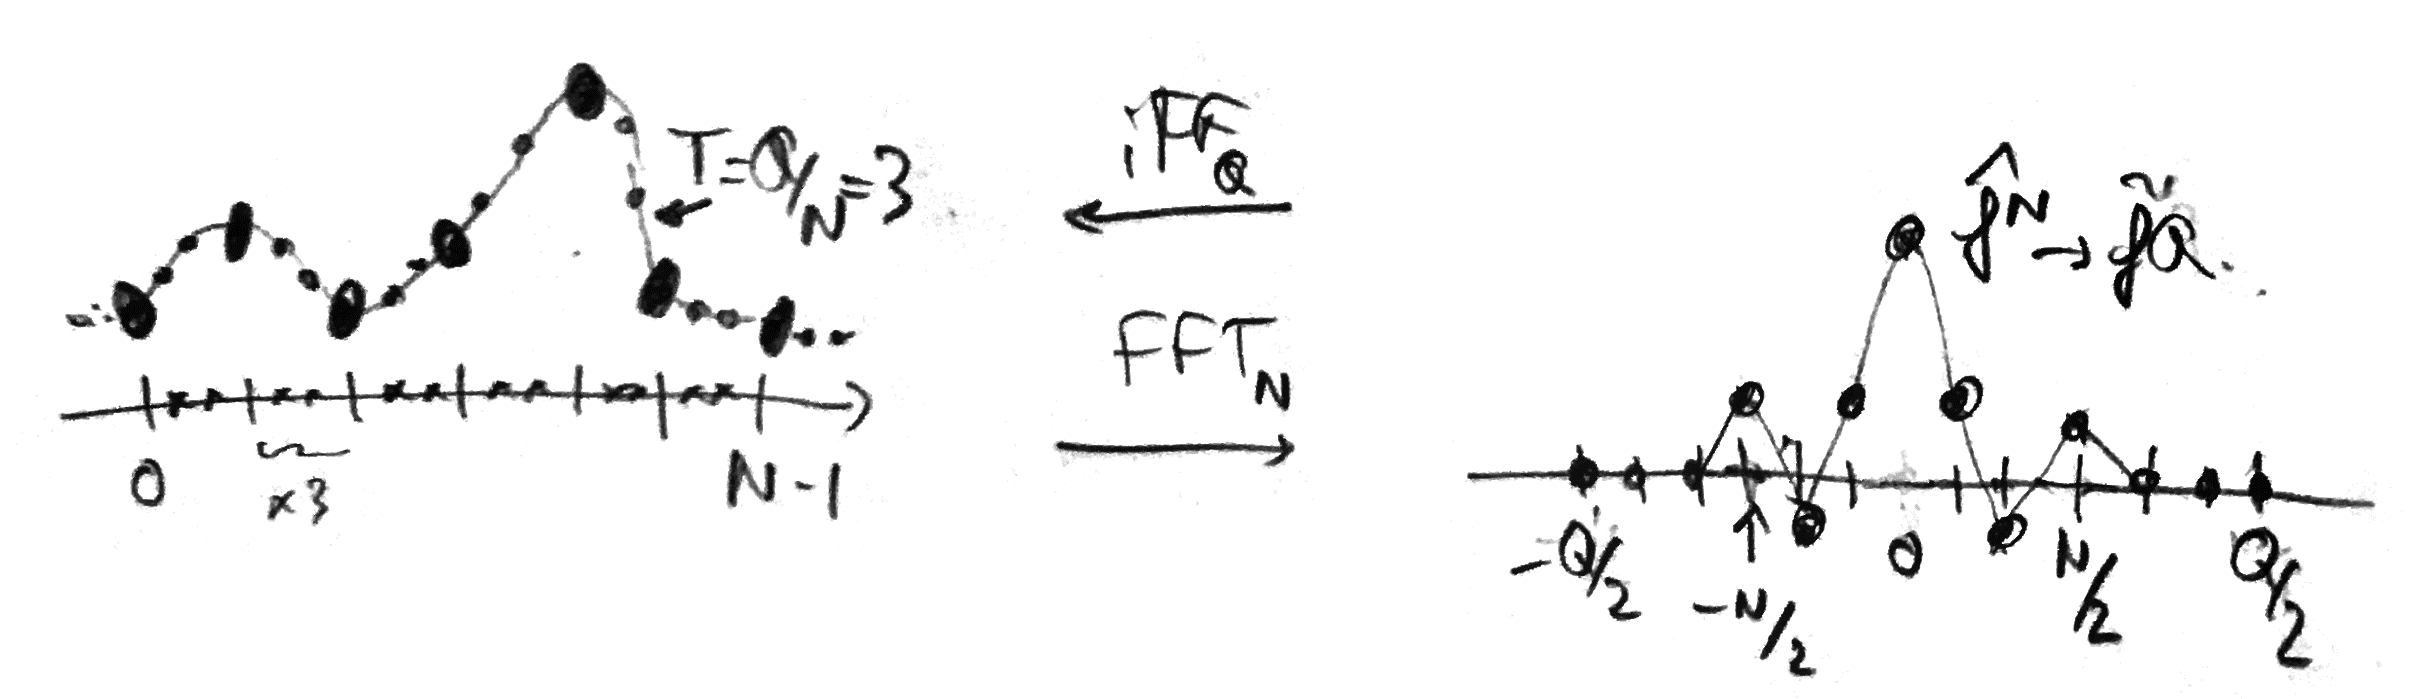
\includegraphics[width=.75\linewidth]{2-fourier/padding-fourier}
\caption{\label{fig-padding-fourier}
Interpolation by zero-padding in the frequency domain.
}
\end{figure}

%%%%%%%%%%%%%%%%%%%%%%%%%%%%%%%%%%%%%%%%%%%%%%%%
%%%%%%%%%%%%%%%%%%%%%%%%%%%%%%%%%%%%%%%%%%%%%%%%
%%%%%%%%%%%%%%%%%%%%%%%%%%%%%%%%%%%%%%%%%%%%%%%%
\section{Fourier in Multiple Dimensions}
\label{sec-fourier-multiple-dim}

The Fourier transform is extended from 1-D to arbitrary finite dimension $d>1$ by tensor product. 


%%%%%%%%%%%%%%%%%%%%%%%%%%%%%%%%%%%%%%%%%%%%%%%%
\subsection{On Continuous Domains}

%%%
\paragraph{On $\RR^d$.}

\wrapf{2-fourier/wave}{2-D sine wave.}
The crux of the power of Fourier transform in arbitrary dimension is that a product of elementary 1-D sine waves is still a sine wave
\eq{
	\prod_{\ell=1}^d e^{ \imath x_\ell \om_\ell } = e^{ \imath \dotp{x}{\om} }
}
moving orthogonally to the wave vector $\om=(\om_\ell)_{\ell=1}^d \in \RR^d$. Here $\dotp{x}{\om} = \sum_\ell x_\ell \om_\ell$ is the canonical inner product on $\RR^d$. 

The definition of the Fourier transform and its inverse are 
\begin{align*}
	\foralls \om \in \RR^d, \quad \hat f(\om) &\eqdef \int_{\RR^d} f(x) e^{-\imath\dotp{x}{\om}} \d x, \\
	\foralls x \in \RR^d, \quad  f(x) &= \frac{1}{(2\pi)^d} \int_{\RR^d} f(x) e^{\imath\dotp{x}{\om}} \d \om,
\end{align*}
under hypotheses of integrability matching exactly those in 1-D.


\myfigure{
\image{orthobases}{.3}{2d-extension-fourier-plane}
\image{orthobases}{.2}{2d-extension-fourier-1}
\image{orthobases}{.2}{2d-extension-fourier-2}
\image{orthobases}{.2}{2d-extension-fourier-3}
}{%
	2D Fourier orthogonal bases. %	
}{fig-2d-fourier-extension}


%%%
\paragraph{On $(\RR/2\pi\ZZ)^d$.}

Given an Hilbertian basis $(\phi_{n_1})_{n_1 \in \NN}$ of $L^2(\XX)$, one construct an Hilbertian basis of $L^2(\XX^d)$ by tensorization
\eql{\label{eq-tensor-product}
	\foralls n=(n_1,\ldots,n_d) \in \NN^d, \quad
	\foralls x \in \XX^d, \quad
	\phi_n(x) = \phi_{n_1}(x_1) \ldots \phi_{n_d}(x_d).
}
Orthogonality is simple to check, and one can also prove convergence for sum of the form $\sum_{\norm{n}_\infty \leq N} \dotp{f}{\phi_n} \phi_n \rightarrow f$ in $L^2(\XX^d)$.

%%% FIG %%%
\wrapf{2-fourier/torus}{The 2-dimensional torus $\TT^2=(\RR/2\pi\ZZ)^2$}
%%%
For the multi-dimensional torus $(\RR/2\pi\ZZ)^d$, using the Fourier basis~\eqref{eq-fourier-basis-1d}, this leads to consider the basis
\eq{
	\foralls n \in \RR^d, \quad \phi_n(x) = e^{\imath \dotp{x}{n}}
} 
which is indeed an Hilbertian orthonormal basis for the inner product $\dotp{f}{g} \eqdef \frac{1}{(2\pi)^d} \int_{\TT^d} f(x)\bar g(x)\d x$. 
%
This defines the Fourier transform and the reconstruction formula on $L^2(\TT^d)$
\eq{
	\hat f_n \eqdef \frac{1}{(2\pi)^d} \int_{\TT^d} f(x) e^{-\imath \dotp{x}{n}}  \d x
	\qandq
	f = \sum_{n \in \ZZ^d} \hat f_n e^{\imath \dotp{x}{n}}.
}

%%%%%%%%%%%%%%%%%%%%%%%%%%%%%%%%%%%%%%%%%%%%%%%%
\subsection{On Discrete Domains}
\label{sec-fft-2d}

%%%%
\paragraph{Discrete Fourier Transform.}

\wrapf{2-fourier/torus-discr}{Discrete 2-D torus.}
On $d$-dimensional discrete domain of the form
\eq{
	n = (n_1,\ldots,n_d) \in \YY_d \eqdef \range{1,N_1} \times \ldots \times \range{1,N_d}
}
(we denote $\range{a,b} \eqdef \enscond{i \in \ZZ}{a \leq i \leq b}$)
of $N=N_1\ldots N_d$ points, with periodic boundary conditions, one defines an orthogonal basis $(\phi_k)_k$ by the same tensor product formula as~\eqref{eq-tensor-product} but using the 1-D discrete Fourier basis~\eqref{eq-dft}
\eql{\label{eq-exp-four-disc-multid}
	\foralls (k,n) \in \YY_d^2, \quad
	\phi_k(n) = \phi_{k_1}(n_1) \ldots \phi_{k_d}(n_d) 
	= \prod_{\ell=1}^d e^{\frac{2\imath\pi}{N_\ell} k_\ell n_\ell}
	= e^{ 2\imath\pi \dotp{k}{n}_{\YY_d} } 	
} 
where we used the (rescaled) inner product
\eql{\label{eq-inner-prod-multi-d}
	\dotp{k}{n}_{\YY_d} \eqdef \sum_{\ell=1}^d \frac{k_\ell n_\ell}{N_\ell}.
}
The basis $(\phi_k)_k$ is indeed orthonormal for this inner product. The Fourier transform gathers inner products in this basis, and (similarly to the 1-D case) the convention is to not normalize them with $(N_\ell)_\ell$, so that 
\begin{align*}
	\foralls k \in \YY_d, \quad 
	\hat f_k &\eqdef \sum_{n \in \YY_d} f_n e^{ -\imath \dotp{k}{n}_{\YY_d} }, \\
	\foralls n \in \YY_d, \quad 
	f_n &= \frac{1}{N} \sum_{k \in \YY_d} \hat f_k e^{ \imath \dotp{k}{n}_{\YY_d} }.
\end{align*}



%%%%
\paragraph{Fast Fourier Transform.}

We detail the algorithm in dimension $d=2$ for notation simplicity, but this extends similarly in arbitrary dimension. 
%
The general idea is that if a fast algorithm is available to compute ortho-decompositions on two 1-D bases $(\phi_{k_1}^{1})_{k_1=1}^{N_1}$, $(\phi_{k_2}^{2})_{k_2=1}^{N_2}$, is extended to compute decomposition on the tensor product basis 
$(\phi_{k_1}^{1} \otimes \phi_{k_2}^{2})_{k_1,k_2}$ by apply succesively the algorithm on the ``rows'' and then ``columns'' (the order does not matters) of the matrix $(f_n)_{n=(n_1,n_2)} \in \RR^{N_1 \times N_2}$. 
%
Indeed
\eq{
	\foralls k=(k_1,k_2), \quad
	\dotp{f}{\phi_{k_1}^{1} \otimes \phi_{k_2}^{2}}
	= \sum_{n=(n_1,n_2)} f_{n} \phi_{k_1}^{1}(n_1) \phi_{k_1}^{1}(n_2) =
	\sum_{n_1} \pa{
		\sum_{n_2} f_{n_1,n_2}  \phi_{k_1}^{1}(n_2)
	} \phi_{k_1}^{1}(n_1).
}
Denoting $C(N_1)$ the complexity of the 1-D algorithm on $\RR^{N_1}$, the complexity of the resulting 2-D decomposition is $N_2 C(N_1)+N_1 C(N_2)$, and hence for the FFT, it is $O(N_1 N_2 \log(N_1 N_2))=O(N \log(N))$ for $N=N_1 N_2$.

If we represent $f \in \RR^{N_1 \times N_2}$ as a matrix, and denote $F_N=(e^{-\frac{2\imath\pi}{N}}kn)_{k,n}$ the Fourier transform matrix (or the matrix where rows are the $\phi_k^*$), then one can compute the 2-D Fourier transform as matrix-matrix products
\eq{
	\hat f = F_{N_1} \times f \times F_{N_2}^* \in \RR^{N_1 \times N_2}.
}
But of course these multiplications are not computed explicitly (one uses the FFT).

\myfigure{
\tabquatre{
\image{fourier}{.24}{fourier-2d-image}&
\image{fourier}{.24}{fourier-2d-fft}&
\image{fourier}{.24}{fourier-2d-masked}&
\image{fourier}{.24}{fourier-2d-masked-fft}
}
}{%
	2D Fourier analysis of a image (left), and attenuation of the periodicity artifact using masking (right). %	
}{fig-fourier-2d}


\texttt{Associated code: coding/test\_fft2.m}


%%%%%%%%%%%%%%%%%%%%%%%%%%%%%%%%%%%%%%%%%%%%%%%%
\subsection{Shannon sampling theorem.}

The sampling Theorem~\ref{thm-shannon-sampling} extends easily to $\RR^d$ by tensorization, assuming that the sampling is on a uniform Cartesian grid. In 2-D for instance, if $\supp(\hat f) \subset [-\pi/s_1,\pi/s_1] \times [-\pi/s_2,\pi/s_2]$ and $f$ is decaying fast enough, 
\eq{
		\foralls x \in \RR^2, \quad 
		f(x) = \sum_{n \in \ZZ^2} f(n_1 s_1,n_2 s_2) \sinc(x_1/s_1-n_1) \sinc(x_2/s_2-n_2) \qwhereq
		\sinc(u) = \frac{\sin(\pi u)}{\pi u}.
}
	

%%%%%%%%%%%%%%%%%%%%%%%%%%%%%%%%%%%%%%%%%%%%%%%%
\subsection{Convolution in higher dimension.}

Convolution on $\XX^d$ with $\XX=\RR$ or $\XX=\RR/2\pi\ZZ$ are defined in the very same way as in 1-D~\eqref{eq-convol-1d} as
\eq{
	f \star g(x) = \int_{\XX^d} f(t) g(x-t) \d t. 
}
Similarly, finite discrete convolution of vectors $f \in \RR^{N_1 \times N_2}$ extend formula~\eqref{eq-finite-convol} as
\eq{
	\foralls n \in \range{0,N_1-1} \times \range{0,N_2-1}, \quad
	(f \star g)_n \eqdef \sum_{k_1=0}^{N_1-1} \sum_{k_2=0}^{N_2-1} f_k g_{n-k}  
}
where additions and subtractions of vectors are performed modulo $(N_1,N_2)$.

The Fourier-convolution theorem is still valid in all this cases, namely $\Ff(f \star g)=\hat f \odot \hat g$. In the finite case, this offers a fast $O(N \log(N))$ method to compute convolutions even if $f$ and $g$ do not have small support.


%%%%%%%%%%%%%%%%%%%%%%%%%%%%%%%%%%%%%%%%%%%%%%%%
%%%%%%%%%%%%%%%%%%%%%%%%%%%%%%%%%%%%%%%%%%%%%%%%
%%%%%%%%%%%%%%%%%%%%%%%%%%%%%%%%%%%%%%%%%%%%%%%%
\section{Application to ODEs and PDEs}
\label{sec-fourier-pdes}

%%%%%%%%%%%%%%%%%%%%%%%%%%%%%%%%%%%%%%%%%%%%%%%%
\subsection{On Continuous Domains}

We here give only the intuition without formal proofs.

One $\XX=\RR$ or $\TT$, one has
\eq{
	\Ff( f^{(k)} )(\om) = (\imath \om)^k \hat f(\om). 
}
Intuitively, $f^{(k)} = f \star \de^{(k)}$ where $\de^{(k)}$ is a distribution with Fourier transform $\hat \de^{(k)}(\om) = (\imath \om)^k$. 
%
Similarly on $\XX=\RR^d$ (see Section~\ref{sec-fourier-multiple-dim} for the definition of the Fourier transform in dimension $d$), one has
\eql{\label{eq-lapl-fourier}
	\Ff(\Delta f)(\om) = -\norm{\om}^2 \hat f(\om)
}
(and similarly on $\TT$ replacing $\om$ by $n \in \ZZ^d$).
%
The Fourier transform (or Fourier coefficients) are thus powerful to study linear differential equations with constant coefficients, because they are turned into algebraic equations.

\begin{figure}
\centering
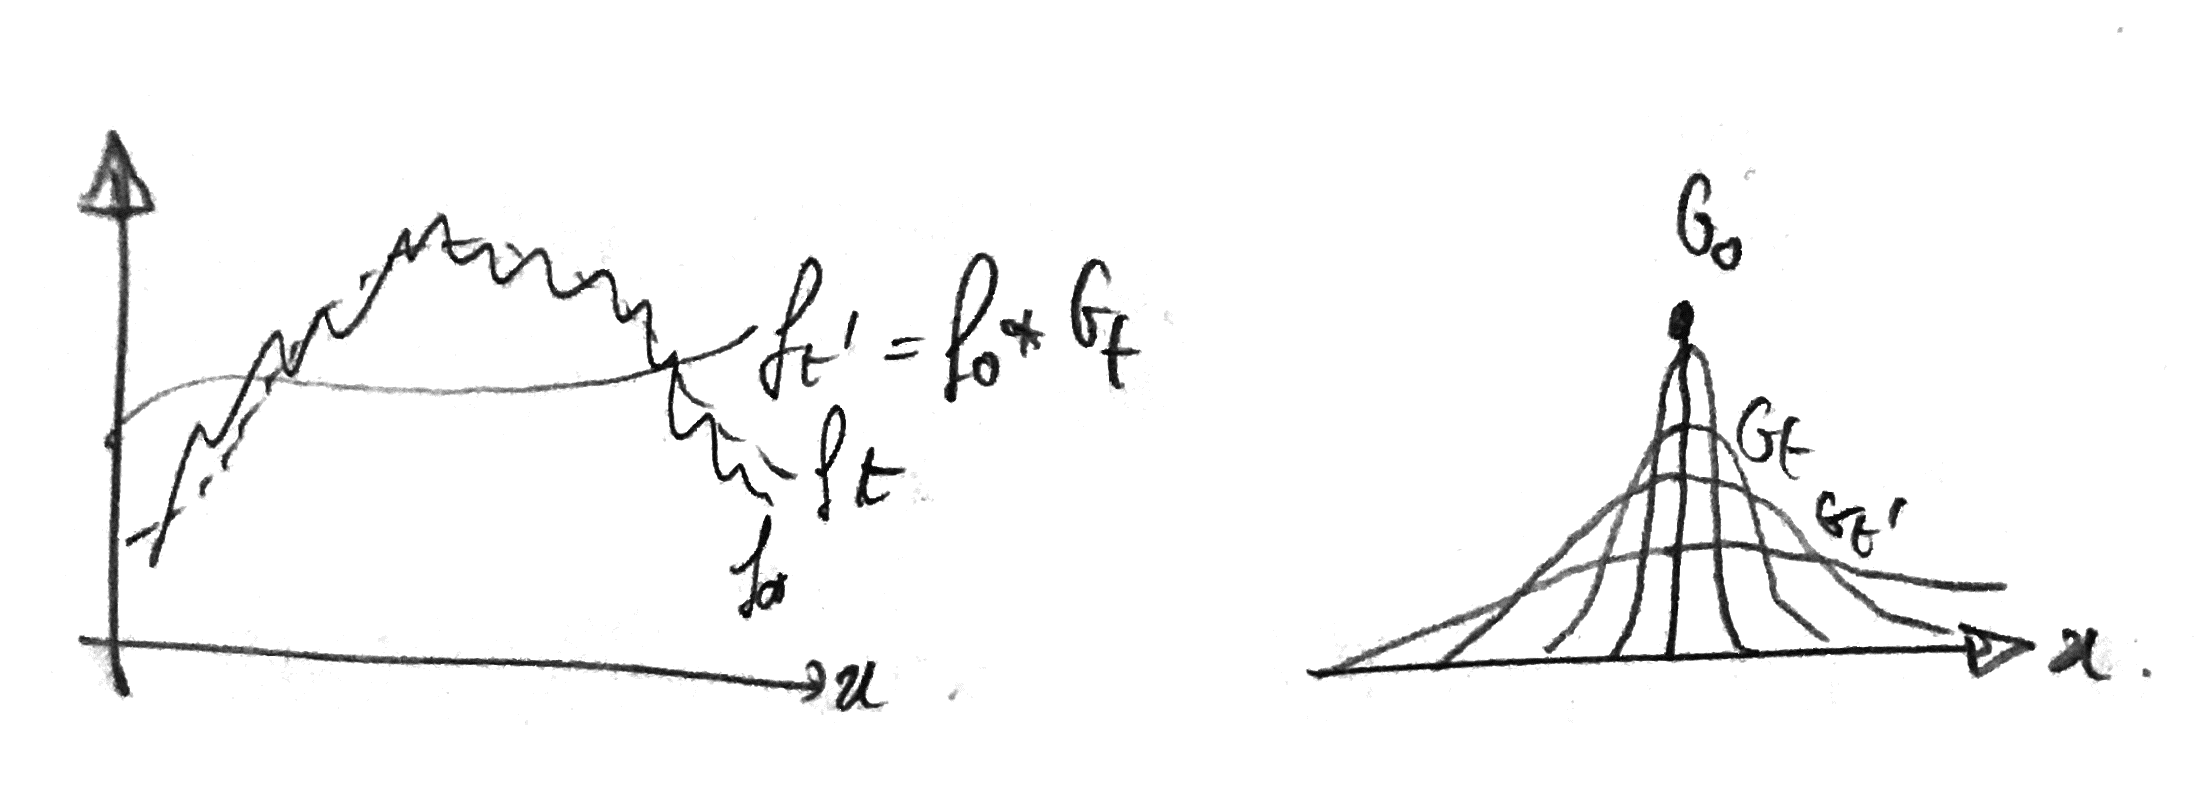
\includegraphics[width=.5\linewidth]{2-fourier/heat}
\caption{\label{fig-heat}
Heat diffusion as a convolution.
}
\end{figure}

As a typical example, we consider the heat equation
\eq{
	\frac{\partial f_t}{\partial t} = \Delta f_t
	\qarrq
	\foralls \om, \quad \frac{\partial \hat f_t(\om)}{\partial t} = -\norm{\om}^2 \hat f(\om).
}
This shows that $\hat f_t(\om) = \hat f_0(\om) e^{-\norm{\om}^2 t}$ and by inverse Fourier transform and the convolution theorem
\eq{
	f_t = G_t \star f_0 \qwhereq
	G_t=\frac{1}{(4\pi t)^{d/2}} e^{-\frac{\norm{x}^2}{4t}}
}
which is a Gaussian of standard deviation $\sqrt{2t}$.


%%%%%%%%%%%%%%%%%%%%%%%%%%%%%%%%%%%%%%%%%%%%%%%%
\subsection{Finite Domain and Discretization}

On $\RR/N\ZZ$ (i.e. discrete domains with periodic boundary conditions), one typically considers forward finite differences (first and second order)
\begin{align}\label{eq-disc-diff-1}
	D_1 f &\eqdef N (f_{n+1}-f_n)_n = f \star d_1 \qwhereq d_1 = [1,0,\ldots,0,-1]^\top \in \RR^N, \\
	\label{eq-disc-diff-2}
	D_2 f = D_1^\top D_1 f & \eqdef N^2 (f_{n+1}+f_{n-1}-2f_n)_n = f \star d_2 \qwhereq d_2 = d_1 \star \bar d_1 = [-2,1,0,\ldots,0,1]^\top \in \RR^N.
\end{align}
\wrapf{2-fourier/finite-diff}{Comparison of the spectrum of $\De$ and $D_2$. }
Thanks to Proposition~\ref{prop-tfd-conv}, one can alternatively computes
\eql{\label{eq-fft-lapl}
	\Ff( D_2 f ) = \hat d_2 \odot \hat f
	\qwhereq
	(\hat d_2)_k = N^2 ( e^{\piN} + e^{-\piN} - 2 ) = -4N^2 \sin\pa{\frac{\pi k}{N}}^2.
}
For $N \gg k$, one thus has $(\hat d_2)_k \sim -(2\pi k)^2$ which matches the scaling of~\eqref{eq-lapl-fourier}. 


%%%%%%%%%%%%%%%%%%%%%%%%%%%%%%%%%%%%%%%%%%%%%%%%
%%%%%%%%%%%%%%%%%%%%%%%%%%%%%%%%%%%%%%%%%%%%%%%%
%%%%%%%%%%%%%%%%%%%%%%%%%%%%%%%%%%%%%%%%%%%%%%%%
\section{A Bit of Group Theory}

The reference for this section is~\cite{peyre2004algebre}.

%%%%%%%%%%%%%%%%%%%%%%%%%%%%%%%%%%%%%%%%%%%%%%%%
\subsection{Characters}

For $(G,+)$ a commutative group, a character is a group morphism $\chi : (G,+) \rightarrow (\CC^*,\cdot)$, i.e. is satisfies
\eq{
	\foralls (n,m) \in G, \quad \chi(n+m) = \chi(n)\chi(m).
}
The set of characters is the so-called dual $(\hat G,\odot)$ and is a group for the pointwise multiplication $(\chi_1 \odot \chi_2)(n) \eqdef \chi_1(n) \chi_2(n)$.  Indeed, the inverse of a character $\chi$ is $\chi^{-1}(n)=\chi(-n)$.

Note that for a finite group $G$ with $|G|=N$, then since $N \times n=0$ for any $n \in G$, then $\chi(n)^N=\chi(N n)=\chi(0)=1$, so that characters assume values in the unit circle, and more precisely
\eql{\label{eq-char-finite-group}
	\chi(n) \in \enscond{ e^{\piN k} }{ 0 \leq k \leq N-1 }.
}
So in particular $\hat G$ is a finite group (since there is a finite number of application between two finite sets) and $\chi^{-1}=\bar\chi$. In the case of a cyclic group, the dual is actually simple to describe.

\begin{prop}\label{prop-iso-cyclic}
	For $G=\ZZ/N\ZZ$, then $\hat G=( \phi_k )_{k=0}^{N-1}$ where $\phi_k=( e^{\piN nk} )_n$ and $k \mapsto \phi_k$ defines a (non-canonical) isomorphism $G \sim \hat G$. 
\end{prop}
\begin{proof}
	The $\phi_k$ are indeed characters.
	
	Conversely, for any $\chi \in \hat G$, according to~\eqref{eq-char-finite-group}, $\chi(1)=e^{\piN k}$ for some $k$. Then 
	\eq{
		\chi(n)=\chi(1)^n=^{\piN k n} = \phi_k(n).
	}
	Note that all these applications are different (because $\phi_k(1)$ are all distincts) which shows that $|G|=|\hat G|$ so that they are isomorphic. 
\end{proof}

This proposition thus shows that characters of cyclic groups are exactly the discrete Fourier orthonormal basis defined in~\eqref{eq-dft}. 


%%%
\paragraph{Commutative groups.}

For more general commutative groups with a finite number of generators, according to the celebrated structure theorem, one can ``decompose'' them as a product of cyclic group (which are in some sense the basic building blocks), i.e. there is the following isomorphism of groups
\eql{\label{eq-structure}
	G \sim (\ZZ/N_1\ZZ) \times \ldots \times (\ZZ/N_d\ZZ) \times \ZZ^Q.
}
If $G$ is finite, then $Q=0$ and $N=N_1 \times N_d$. In this case, $G$ is simply a discrete $d$-dimensional ``rectangle'' with periodic boundary conditions. 

For two finite groups $(G_1,G_2)$ one has 
\eql{\label{eq-iso-product-char}
	\widehat{G_1 \times G_2} = \hat G_1 \otimes \hat G_2 = \enscond{ \chi_1 \otimes \chi_2 }{ (\chi_1,\chi_2) \in \hat G_1 \times \hat G_2 }.
} 
Here $\otimes$ is the tensor product of two functions
\eq{
	\foralls (n_1,n_2) \in G_1 \times G_2, \quad
	(\chi_1 \otimes \chi_2)(n_1,n_2) \eqdef \chi_1(n_1)\chi_2(n_2).
}
Indeed, one verifies that $\chi_1 \otimes \chi_2$ is a morphism, and in fact one has the factorization $\chi=\chi(\cdot,0) \otimes \chi(0,\cdot)$ because one decomposes $(n_1,n_2)=(n_1,0)+(0,n_2)$. 

This construction, thanks to the structure theorem, leads to a constructive proof of the isomorphism theorem.

\begin{prop}
	If $G$ is commutative and finite then $\hat G \sim G$.
\end{prop}
\begin{proof}
	The structure theorem~\eqref{eq-structure} for $Q=0$ and the dual of a product~\eqref{eq-iso-product-char} shows that 
	\eq{
		\hat G \sim \hat G_1 \otimes \ldots \otimes \hat G_d
	} 
	where we denoted $G_\ell \eqdef \ZZ/N_\ell\ZZ$. 
	%
	One then remark that  $\hat G_1 \otimes \hat G_2 \sim \hat G_1 \times \hat G_2$.
	%
	One concludes thanks to Proposition~\ref{prop-iso-cyclic}, since one has $\hat G_k \sim G_k$.
\end{proof}

Note that the isomorphism $\hat G \sim G$ is not ``canonical'' since it depends on the indexing of the roots of unity on the circle. Similarly to the case of duality of vector space, the isomorphism $\hat{\hat{G}} \sim G$ can be made canonical by considering the evaluation map
\eq{
	g \in G \longmapsto e_g \in \hat{\hat{G}}
	\qwhereq
	\pa{
	e_g : \chi \in \hat G \mapsto \chi(g) \in \CC^*.
	}
}

%%%
\paragraph{Discrete Fourier transform from character's point of view.}

One can be even more constructive by remarking that characters in $\hat G_\ell$ are the discrete Fourier atoms~\eqref{eq-dft}, i.e. are of the form 
\eq{
	( e^{\frac{2\imath\pi}{N_\ell} k_\ell n_\ell})_{n_\ell=0}^{N_\ell-1}
	\quad\text{for some}\quad
	0 \leq k_\ell < N_\ell.
} 
Identifying $G$ and $G_1 \times \ldots \times G_d$, 
by tensorizing these functions together, one thus obtains that the characters composing $\hat G$ are exactly the orthogonal multi-dimensional discrete Fourier basis~\eqref{eq-exp-four-disc-multid}.

%%%%%%%%%%%%%%%%%%%%%%%%%%%%%%%%%%%%%%%%%%%%%%%%
\subsection{More General cases}

%%%
\paragraph{Infinite groups.}

For an infinite group with a finite number of generator, one has  $Q>0$, and the definition of $\hat G$ should impose the continuity of the characters (and also use an invariant measure on $G$ to define inner products). In the case $G=\ZZ$, the dual are indexed by a continuous parameter, 
\eq{
	\hat \ZZ = \enscond{ \phi_\om : n \mapsto e^{\imath n \om} \in \CC^\ZZ }{  \om \in \RR/2\pi\ZZ }
}
so that $\hat \ZZ \sim \RR/2\pi\ZZ$.
%
The case $G=\ZZ^Q$ follows by tensorization. 
%
The $(\phi_\om)_\om$ are ``orthogonal'' in the sense that $\dotp{\phi_\om}{\phi_{\om'}}_\ZZ = \de(\om-\om')$ can be understood as a Dirac kernel (this is similar to the Poisson formula), where $\dotp{u}{v}_\ZZ \eqdef \sum_n u_n \bar v_n$. 
%
The ``decomposition'' of a sequence $(c_n)_{n \in \ZZ}$ on the set of characters is equivalent to forming a Fourier series $\sum_n c_n e^{-\imath n \om}$. 

Similarly, for $G=\RR/2\pi\ZZ$, one has $\hat G=\ZZ$, with orthonormal characters $\phi_n=e^{\imath \cdot n}$, so that the decomposition of functions in $L^2(G)$ is the computation of Fourier coefficients.
%
Intuitively, an Hilbertian theory is associated to a compact group, which comes with an invariant measure. 

%%%
\paragraph{Non-commutative groups.}
 
For non-commutative group, one observes that $G$ is not isometric to $\hat G$. A typical example is the symmetric group $\Si_N$ of $N$ elements, where one can show that $\hat G = \{\Id,\epsilon\}$ where $\epsilon(\si) = (-1)^{q}$ is the signature, where $q$ is the number of permutations involved in a decomposition of $\si \in \Si_N$. 

In order to study non-commutative groups, one has to replace morphisms $\chi : G \rightarrow \CC^*$ by morphisms $\rho : G \rightarrow \text{GL}(\CC^{n_\rho})$ for some $n_\rho$, which are called ``representations'' of the group $G$. For $(g,g') \in G$ (denoting now multiplicatively the operation on $G$), one should thus have $\rho(gg')=\rho(g) \circ \rho(g')$. When $n_\rho=1$, identifying $\text{GL}(\CC) \sim \CC^*$, one retrieves the definition of characters. Note that if $\rho$ is a representation, then $\chi(g) \eqdef \tr(\rho(g))$, where $\tr$ is the trace, defines a character. 

If there is a subspace $V$ stable by all the $\rho(g)$, one can build $W$ such that $\RR^{n_\rho}=V+W$ which is also stable, thus reducing the study of $\rho$ to the study on a small space (matrices have a block diagonal form). It suffice to consider the inner product
\eq{
	\dotp{x}{y} \eqdef \sum_{g \in G} \dotp{\rho(g)x}{\rho(g)y}_{\RR^{n_\rho}}
}
and select the orthogonal $V^\bot$ for this product. Note that when using an ortho-basis of $\RR^{n_\rho}$ for this inner product, the matrices associated to the $\rho(g)$ are unitary.
%
In order to limit the set of such representations, one is only interested in ``elementary'' ones, which does not have invariant sub-spaces, and are called ``irreducible'' (otherwise one could create arbitrary large representation by stacking others in a block diagonal way). 
%
One also only consider these irreductible representation up to isomorphism, where two representation $(\rho,\rho')$ are said to be isomorphic if $\rho(g) = U^{-1} \rho(g) U$ where $U \in \text{GL}(\CC^d)$ is a change of basis. The set of all these representations up to isomomorphisms is called the dual group and denoted $\hat G$.

For the symmetric group, there is an explicit description of the set of irreducible representations.  
%
For instance, for $G=\Sigma_3$, $|G|=6$, and there is two representation of dimension 1 (the identity and the signature, which are the caracters) and one representation of dimension 2, which is obtained by identifying $G$ with the isometric of the equilateral triangle in $\RR^2$, and the dimensions indeed satisfy $6 = |G| = \sum n_\rho^2 = 1+1+2^2$. 

One can show that the dimensions $n_\rho$ of these irreducible representations $\rho \in \hat G$ satisfies $\sum_{\rho \in \hat G} n_\rho^2 = N$ and that the entries of the matrices involved in these representation define an orthogonal basis of the space of functions $f : G \rightarrow \CC$ (note however that this set of basis function is not canonical since it depends on a particular choice of basis for each representation up to isomorphism).
%
The associated Fourier transform of a function $f : G \rightarrow \Cc$ is defined as
\eq{
	\foralls \rho \in \hat G, \quad
	\hat f(\rho) \eqdef \sum_{g \in G} f(g) \rho(g) \in \CC^{n_\rho \times n_\rho}.  
}
This corresponds to computing inner products with the aforementioned ortho-basis.
%
It is an invertible linear transform, whose invert is given next.

\begin{prop}
One has
\eq{
	\foralls g \in G, \quad
	f(g) = \frac{1}{|G|} \sum_{\rho \in \hat G} n_\rho \tr( \hat f(\rho) \rho(g^{-1}) ). 
}
\end{prop}
\begin{proof}
The proof relies on the following formula, which states that for any $g \in G$
\eq{
	A_g \eqdef \sum_{\rho \in \hat G} n_\rho \tr( \rho(g) ) = \de_g
}
where $\de_g=0$ for $g \neq \Id_G$ and $\de_{\Id_G}=1$. We will not prove this formula, and refer to the book of Diaconis p.13 for a proof, which is based on the decomposition of the character of the so-called standard representation (which corresponds to permuting by the action of $G$ the canonical basis of $\RR^{|G|}$) on the set of characters, which are orthogonal. 
%
One then has 
\begin{align*}
	\frac{1}{|G|} \sum_{\rho \in \hat G} n_\rho \tr( \hat f(\rho) \rho(g^{-1}) ) 
	&=  \frac{1}{|G|} \sum_{\rho \in \hat G} n_\rho \tr( \sum_u f(u) \rho(u) \rho(g^{-1}) ) \\
	&=  \sum_u  f(u) \frac{1}{|G|}  \sum_{\rho \in \hat G} n_\rho \tr( \rho(u g^{-1}) )
	=  \sum_u  f(u) G_{ug^{-1}} = f(g).
\end{align*}
\end{proof}





One can define the convolution of two functions $f,h : G \rightarrow \CC$ as
\eq{
	(f \star h)(a) \eqdef \sum_{bc=a} f(b) h(c)
}
(beware that it is not commutative anymore). The Fourier transform diagonalize these convolution operators, has stated next.

\begin{prop}
Denoting $\Ff(f) = \hat f$
\eq{
	\Ff(f \star h)(\rho) = \hat f(\rho) \times \hat h(\rho)
}
where $\times$ is the matrix multiplication.
\end{prop}
\begin{proof}
\eq{
	\Ff(f \star h)(\rho) = \sum_x \sum_y f(y) h(y^{-1}x) \rho(y y^{-1} x) = \sum_x \sum_y f(y) \rho(y) h(y^{-1}x) \rho(y^{-1}x) 
	= \sum_y f(y) \rho(y) \sum_z h(z) \rho(z)
}
where we made the change of variable $z=y^{-1}x$.
\end{proof}


For certain groups, there exists fast Fourier transforms to compute $\hat f$, an example being the permutation group, but the structure of these algorithm is much more involved than in the case $G=\ZZ/N\ZZ$. 

This theory extends to compact group by considering a discrete but infinite set of representations. A typical example is to analyze signals defined on the rotation groups SO$(3)$, on which one can compute explicitly the representation using the basis of sphereical harmonics detailed in Section~\ref{sec-spherical-harm} bellow. In this case, one has a representation of dimension $2\ell+1$ for each frequency index $\ell$. 
 
%
% It is possible to lift the 3-D sphere $\SS^2$ on the group SO$(3)$ since it operate transitively on the sphere, for instance defining for $f : \SS^2 \rightarrow \CC$ its lifted version $f_L(g) = f(g(o))$ where $o$ is any point on the sphere. 

%%%%%%%%%%%%%%%%%%%%%%%%%%%%%%%%%%%%%%%%%%%%%%%%
%%%%%%%%%%%%%%%%%%%%%%%%%%%%%%%%%%%%%%%%%%%%%%%%
%%%%%%%%%%%%%%%%%%%%%%%%%%%%%%%%%%%%%%%%%%%%%%%%
\section{A Bit of Spectral Theory}

In order to define Fourier methods on general domains $\XX$, one can use the aforementioned group-theoretic approach if $\XX=G$ is a group, or also if a group acts transitively on $\XX$. An alternative way is to describe the equivalent of Fourier basis functions as diagonalizing a specific differential operator (as we have seen in Section~\ref{sec-fourier-pdes} that it is in some sense a way to characterise the Fourier basis). Of particular interest is the Laplacian, since it is the lowest order rotation-invariant differential operator, and that there exists natural generalization on domains such as surfaces or graphs.


%%%%%%%%%%%%%%%%%%%%%%%%%%%%%%%%%%%%%%%%%%%%%%%%
\subsection{On a Surface or a Manifold}

\wrapf{2-fourier/laplacian-surf}{Computing Laplacian on a surface}
The presentation here is very informal. One can define the Laplacian of a smooth function $f: \XX \rightarrow \CC$ defined on a ``surface'' $\XX$ as
\eq{
	\foralls x \in \XX, \quad
	(\Delta f)(x) \eqdef \lim_{\epsilon \rightarrow 0}  \frac{1}{\text{Vol}(B_\epsilon(x))} \int_{B_\epsilon(x)} f(x) \d \mu(x) - f(x).
}
Here $\mu(x)$ is the area measure on $\XX$, $\text{Vol}(B) \eqdef \int_B \d\mu(x)$, and $B_\epsilon(x) = \enscond{y}{d_\XX(x,y) \leq \epsilon}$ is the geodesic ball of radius $\epsilon$ at $x$, where $d_\XX$ is the geodesic distance on $\XX$ (length of the shortest path). 

If the surface $\XX$ is smooth, compact and connected, then it is possible to show that $\Delta$ is itself a compact operator with a negative spectrum $0 > \la_1 > \la_2 > \ldots$ and an orthogonal set of eigenvectors $(\phi_n)_{n \geq 0}$ where $\phi_1=1$. Here the inner product is $\dotp{f}{g}_\XX \eqdef \int_\XX f(x)g(x) \d\mu(x)$ on $L^2(\XX)$. 
%
In the case of a flat torus $\XX=(\RR/\ZZ)^d$, then writing $x=(x_1,\ldots,x_d)$, 
\eq{
	\De f = \sum_{s=1}^d \frac{\partial^2 f}{\partial^2 x_s}.
} 
Similarly to~\eqref{eq-lapl-fourier} (which was for an unbounded domain), then one can chose for this eigen-functions $\phi_n$ the Fourier basis~\eqref{eq-fourier-basis-1d} and $\la_n=-\norm{n}^2$

%%%%%%%%%%%%%%%%%%%%%%%%%%%%%%%%%%%%%%%%%%%%%%%%
\subsection{Spherical Harmonics}
\label{sec-spherical-harm}

\wrapf{2-fourier/spherical}{Spherical coordinates.}
Of particular interest is the special case of the previous construction on the $(d-1)$-dimensional sphere $\SS^{d-1} = \enscond{x \in \RR^d}{\norm{x}_{\RR^d}=1}$.
% 
In this case, there exists a closed form expression for the eigenvectors of the Laplacian. In the 3-D case $d=3$, they are indexed by $n=(\ell,m)$
\eq{
	\foralls \ell \in \NN, \quad
	\foralls m=-\ell,\ldots,\ell, \quad
	\phi_{\ell,m}(\th,\phi) = e^{\imath m \phi} P_{\ell}^m( \cos(\th) )
}
and then the eigenvalue of the Laplacian is $\la_{\ell,m} = -\ell(\ell+1)$. Here $P_{\ell}^m$ are associated Legendre polynomials, and we used spherical coordinates $x=(\cos(\phi),\sin(\phi)\sin(\th),\sin(\phi)\cos(\th)) \in \SS^3$ for $(\th,\phi) \in [0,\pi] \times [0,2\pi]$.
%
The index $\ell$ is analogous to the amplitude of Fourier frequencies in 2-D. 
%
For a fixed $\ell$, the space $V_\ell = \text{span}( \phi_{\ell,m} )$ is an eigenspace of $\Delta$, and is also invariant under rotation. 
	

%%%%%%%%%%%%%%%%%%%%%%%%%%%%%%%%%%%%%%%%%%%%%%%%
\subsection{On a Graph}

\wrapf{2-fourier/graph}{Weighted graph.}
We assume $\XX$ is a graph of $N$ vertices, simply indexed $\{1,\ldots,N\}$. Its ``geometry'' is described by a connectivity matrix of weights $W=(w_{i,j})_{i \sim j}$ where we denote $i \sim j$ to indicate that $(i,j)$ is an edge of the graph for $(i,j) \in \XX^2$. We assume that this weight matrix and the connectity is symmetric, $w_{i,j}=w_{j,i}$. 

The graph Laplacian $\Delta : \RR^N \rightarrow \RR^N$ is computing the difference between the average of values around a point and the value at this point
\eq{
	\foralls f \in \RR^N, \quad
	(\Delta f)_i \eqdef \sum_{j \sim i} w_{i,j} f_j - (\sum_{j \sim i} w_{i,j}) f_i 
	\qarrq 
	\Delta = W-D
}
where $D \eqdef \diag_i(\sum_{j \sim i} w_{i,j})$. In particular, note $\Delta \ones=0$

For instance, if $\XX = \ZZ/N\ZZ$ with the graph $i \sim i-1$ and $i \sim i+1$ (modulo $N$), then $\De$ is the finite difference Laplacian operator $\De=D_2$ defined in~\eqref{eq-disc-diff-2}. This extends to any dimension by tensorization. 

\begin{prop}
Denoting $G : f \in \RR^N \mapsto ( \sqrt{w_{i,j}} (f_i-f_j) )_{i<j}$ the graph-gradient operator, one verifies that 
\eq{
	-\Delta = G^\top G
	\qarrq
	\foralls f \in \RR^N, \quad 
	\dotp{ \Delta f }{f}_{\RR^N} = -\dotp{Gf}{Gf}_{\RR^{P}}.
}
where $P$ is the number of (ordered) edges $E=\enscond{(i,j)}{i \sim j, i<j}$. 
\end{prop}
\begin{proof}
	One has 
	\begin{align*}
		\norm{Gf}^2 &= \sum_{(i,j) \in E} w_{i,j}|f_i-f_j|^2
				=\sum_{i<j}w_{i,j}f_i^2  + \sum_{i<j}w_{i,j}f_j^2 - 2 \sum_{i<j}w_{i,j}f_i f_j  \\
				&= \sum_{i<j}w_{i,j}f_i^2 + \sum_{i>j}w_{i,j}f_i^2- \sum_{i,j}w_{i,j}f_i f_j
				= \sum_j f_i^2 \sum_{i,j} w_{i,j} - \sum_if_i  \sum_j w_{i,j} f_j \\
				&= \dotp{Df}{f}-\dotp{Lf}{f}=-\dotp{Lf}{f}.
	\end{align*}
\end{proof}

This proposition shows that $\Delta$ is a negative semi-definite operator, which thus diagonalizes in an ortho-basis $(\phi_n)_{n=1}^N$, with $\phi_1=1$, with eigenvalues $0 \geq \la_1 \geq \la_N$. If $\XX$ is connected, one can show that $\la_1 <0$. In the case of a regular graph associated to a uniform grid, one retrieves the discrete Fourier basis~\eqref{eq-dft}. 

More details and application of Laplacians on graphs can be found in Chapter~\ref{chap-meshes}, see in particular Section~\ref{sec-grad-lapl-meshes}.



%%%%%%%%%%%%%%%%%%%%%%%%%%%%%%%%%%%%%%%%%%%%%%%%
\subsection{Other things}

Multiplication of polynomials (\texttt{Code text\_polymult.m}).

Fourier transform for finite-field valued functions.




% !TEX root = ../FundationsDataScience.tex
\chapter{Linear Mesh Processing}
\label{chap-meshes}

This chapter exposes the basics of surface approximation with 3D meshes and the way to process such meshes with linear operators. In particular, it studies filtering on 3D meshes and explains how a Fourier theory can be built to analyze these filters. 

%%%%%%%%%%%%%%%%%%%%%%%%%%%%%%%%%%%%%%%%%%%%%%%%
%%%%%%%%%%%%%%%%%%%%%%%%%%%%%%%%%%%%%%%%%%%%%%%%
%%%%%%%%%%%%%%%%%%%%%%%%%%%%%%%%%%%%%%%%%%%%%%%%
\section{Surface Discretization with Triangulated Mesh}

%%%%%%%%%%%%%%%%%%%%%%%%%%%%%%%%%%%%%%%%%%%%%%%%
\subsection{Continuous Geometry of Surfaces}

In this course, in order to simplify the mathematical description of surfaces, we consider only globally parameterized surfaces. We begin by considering surfaces embedded in euclidean space $\Mm \subset \RR^k$.

\begin{defn}[Parameterized surface] \label{defn-param-surface}A parameterized surface is a mapping
\eq{ u \in \Dd \subset \RR^2 \mapsto \phi(u) \in \Mm.} 
\end{defn}

Of course, most surfaces do not benefit from such a simple parameterization. For instance, a sphere should be split into two parts in order to be mapped on two disks $\Dd_1,\Dd_2$. These topological difficulties require the machinery of manifolds in order to incorporate a set of charts $\Dd = \{\Dd_i\}_i$ that overlap in a smooth manner. All the explanations of this course extend seamlessly to this multi-charts setting.

A curve is defined in parameter domain as a 1D mapping $t \in [0,1] \mapsto \ga(t) \in \Dd$. This curve can be traced over the surface and its geometric realization is $\bar \ga(t) \eqdef \phi(\ga(t)) \in \Mm$. The computation of the length of $\ga$ in ambient $k$-dimensional space $\RR^k$ follows the usual definition, but to do the computation over the parametric domain, one needs to use a local metric defined as follow. 

\begin{defn}[First fundamental form]
For an embedded manifold $\Mm \subset \RR^k$, the first fundamental form is
\eq{
	I_\phi = \pa{ \dotp{\pd{\phi}{u_i}}{\pd{\phi}{u_j}} }_{i,j=1,2}.
}
\end{defn}

This local metric $I_\phi$ defines at each point the infinitesimal length of a curve as 
\eq{
	L(\ga) \eqdef \int_0^1 \norm{ \bar \ga'(t) } \d t
	= \int_0^1 \sqrt{ \transp{\ga'(t)} I_\phi(\ga(t)) \ga'(t) } \d t.
}
This fundamental form is an intrinsic invariant that does not depends on how the surfaces is isometrically embedded in space (since the length depends only on this tensor field $I_\phi$). In contrast, higher order differential quantities such as curvature might depend on the bending of the surface and are thus usually not intrinsic (with the notable exception of invariants such as the gaussian curvature). In this course, we restrict ourselves to first order quantities since we are mostly interested in lengths and the intrinsic study of surfaces.  


\begin{exmp}[Isometry and conformality]
A surface $\Mm$ is locally isometric to the plane if $I_\phi = \Id_2$. This is for instance the case for a cylinder. The mapping $\phi$ is said to be conformal if $I_\phi(u) = \la(u)\Id_2$. It means that the length of a curve over the plane is only locally scaled when mapped to the surface. In particular, the angle of two interescting curves is the same over the parametric domain and over the surface. This is for instance the case for the stereographic mapping between the plane and a sphere.
\end{exmp}

%%%%%%%%%%%%%%%%%%%%%%%%%%%%%%%%%%%%%%%%%%%%%%%%
\subsection{Discretization of Surfaces with Triangulations}
\label{subsec-mesh-structure}

\paragraph{Mesh Data Structure}

A triangulated mesh is a discrete structure that can be used to approximate a surface embedded in Euclidean space $\RR^k$. It is composed of a topological part $M=(V,E,F)$ and a geometrical realization $\Mm=(\Vv,\Ee,\Ff)$. It is important to make the distinction between these two parts since many algorithms rely only on geometry (point clouds processings such as dimension reduction) or on topology (such as compression).

The topology $M$ of the mesh is composed of
\begin{rs}
	\item \textit{Vertices} (0D): this is an abstract set of indices $V \simeq \{1,\ldots,n\}$.
	\item \textit{Edges} (1D): this is a set of pair of vertices $E \subset V \times V$. This set is assumed to be symmetric
		\eq{ (i,j) \in E \quad\Longleftrightarrow \quad i \sim j \Leftrightarrow (j,i) \in E. }
	\item  \textit{Faces} (2D): this is a collection of 3-tuples of vertices $F \subset V \times V \times V$, with the additional 
		compatibility condition
		\eq{ (i,j,k) \in F \quad\Longrightarrow \quad (i,j), (j,k), (k,i) \in E. }
		We further assumer that there is no isolated edges
		\eq{ \foralls (i,j) \in E, \quad \exists \, k, \; (i,j,k) \in F. }
\end{rs}

The set of edges can be stored in a symmetric matrix $A \in \RR^{n \times n}$ such that $A_{ij}=1$ if $(i,j) \in E$ and $A_{ij}=0$ otherwise. This matrix is often stored as a sparse matrix since the number of edges is usually much smaller than $n^2$. The set of vertices and edges form a non-oriented graph $\Gg=(V,E)$. Faces are often stored as a matrix $A_F \in \{1,\ldots,n\}^{3 \times m}$ where $m$ is the number of faces and a column $((A_F)_{i,1},(A_F)_{i,2},(A_F)_{i,3})$ stores the indices of a face. In a triangulation, the face matrix $A_F$ allows to recover the edge incidence matrix $A$. The face data structure allows to really capture the 2D geometry of surfaces, which is not possible with graphs alone. 

The geometric realization $\Mm$ is defined through a spacial localization of the vertices (for instance in 3D space) 
\eq{
	 \Vv \eqdef \enscond{x_i}{ i \in V } \subset \RR^3.
}
This allows to define a piecewise linear mesh
\eq{ 
	\Ff \eqdef \bigcup_{(i,j,k) \in F} \text{Conv}(x_i,x_j,x_k) \subset \RR^3,
}
where the convex envelop $\text{Conv}(x,y,z)$ of three points is the Euclidean triangle generated by $(x,y,z)$. 

This piecewise linear realization $\Mm$ can be displayed as a 3D surface on a computer screen. This is performed through a perspective projection of the points and a linear interpolation of color and light inside the triangle. Figure \ref{fig-display-3d} shows an example of 3D display, with a zoom on the faces of the mesh.
  
\myfigure{       
\image{meshes}{0.22}{display/elephant-50kv-mesh}
\image{meshes}{0.24}{display/elephant-50kv-mesh-faceted-2}
\image{meshes}{0.24}{display/elephant-50kv-mesh-faceted-4}
\image{meshes}{0.24}{display/elephant-50kv-mesh-faceted-6}
}{
Example of display of a 3D mesh.
}{fig-display-3d}

   
%%%%%%%%%%%%%%%%%%%%%%%%%%%%%%%%%%%%%%%%%%%%%%%%
\paragraph{Adjacency Relationships}

From the basis topological information given by $M = (V,E,F)$, one can deduce several adjacency data-structures that are important to navigate over the triangulation.

\begin{defn}[Vertex 1-ring] The vertex 1-ring of a vertex $i \in V$ is 
\eql{ \label{eq-vertex-1-ring}
	V_i \eqdef \enscond{j \in V}{(i,j) \in E} \subset V. `
}
The $s$-ring is defined by induction as
\eql{\label{eq-iterated-ring}
	\foralls s>1, \quad V_i^{(s)} = \enscond{ j \in V }{ (k,j) \in E \qandq k \in V_i^{(s-1)} }.
}
\end{defn}

\begin{defn}[Face 1-ring] The face 1-ring of a vertex $i \in V$ is 
\eq{ F_i \eqdef \enscond{(i,j,k) \in F}{i,j \in V} \subset F. }
\end{defn}

The geometrical realization of a vertex 1-ring is
\eq{ \Vv_i = \bigcup_{(i,j,k) \in V_i} \text{Conv}(x_i,x_j,x_k).  }
A triangulated mesh is a manifold mesh if all the rings $\Vv_i$ for $i \in V$ are homeomorphic to either a disk (for interior vertices) or to a half disk (for boundary vertices). This ensures that the geometrical mesh really has the topology of a 2D surface embedded in $\RR^3$ (possibly with boundaries). In particular, it implies that there is at most two faces connected to each edge
\eq{ \foralls (i,j) \in E, \quad \#\enscond{k}{ (i,j,k) \in F } \leq 2.}


As an application of these local rings, one can compute a normal at each point using a simple rule
\eq{
\foralls f = (i,j,k) \in F, \quad \overrightarrow{n_f} \eqdef \frac{(x_j-x_i) \wedge (x_k-x_i)}{\norm{(x_j-x_i) \wedge (x_k-x_i)}}.
}
and where
\eq{
\foralls i \in V, \quad \overrightarrow{n_i} \eqdef \frac{ \sum_{f \in F_i} \overrightarrow{n_f} }{ \norm{\sum_{f \in F_i} \overrightarrow{n_f}} }.
}
These normals are used to define for instance a light intensity $I(i) = \max(\dotp{n_i,\ell(i)},0)$, where $\ell(i)$ is the incident light. In practice one uses a infinite light source $\ell(i)=\ell=$constant or a local spot located at position $s \in \RR^3$ through $\ell(i)=(v_i-s)/\norm{v_i-s}$. This light intensity is interpolated on the whole mesh during display. 


%%%%%%%%%%%%%%%%%%%%%%%%%%%%%%%%%%%%%%%%%%%%%%%%
%%%%%%%%%%%%%%%%%%%%%%%%%%%%%%%%%%%%%%%%%%%%%%%%
%%%%%%%%%%%%%%%%%%%%%%%%%%%%%%%%%%%%%%%%%%%%%%%%
\section{Linear Mesh Processing}

The light intensity $I$ is a particular example of a function defined at each vertex of the mesh. Mesh processing is intended to process such functions and we thus define carefully vector spaces and operators on meshes.

%%%%%%%%%%%%%%%%%%%%%%%%%%%%%%%%%%%%%%%%%%%%%%%%
\subsection{Functions on a Mesh}

In this course, a function is a discrete set of values defined at each vertex location.

\begin{defn}[Linear space on a mesh] A function on a mesh is a mapping $f \in \ldeux(\Vv) \simeq \ldeux(V) \simeq \RR^n$ and can be viewed equivalently as 
\eq{
	f: 
	\left\{
		\begin{array}{c c c}
			\Vv & \longrightarrow & \RR\\
			x_i & \longmapsto & f(x_i)
		\end{array}
	\right.
	\quad\Longleftrightarrow\quad
	f: 
	\left\{
		\begin{array}{c c c}
			V & \longrightarrow & \RR\\
			i & \longmapsto & f_i
		\end{array}
	\right.
	\quad\Longleftrightarrow\quad
	f=(f_i)_{i\in V} \in \RR^n.
}
\end{defn}

The linear space of the functions on a mesh is equipped with an Hilbert space structure that allows to quantify approximation error and compute projections of functions.

\begin{defn}[Inner product and norm] One defines the following inner product and norm for vector $f,g \in \RR^n$
\eq{
	\dotp{f}{g} \eqdef \sum_{i \in V} f_i g_i
	\qandq 
	\norm{f}^2 = \dotp{f}{f}.
}
\end{defn}

In order to modify (process) functions on a mesh (such as a light intensity $I$), this course considers only linear operations that are defined through a large matrix.

\begin{defn}[Linear operator $A$] A linear operator $A$ is defined as 
\eq{ 
	A: \ldeux(V) \rightarrow \ldeux(V) 
	\quad\Longleftrightarrow \quad
	A = (a_{ij})_{i,j \in V} \in \RR^{n \times n} \; \text{(matrix)}.
}
and operate on a function $f$ as follow
\eq{
	(A f)(x_i) = \sum_{j \in V} a_{ij} f(x_j)
	\Longleftrightarrow \quad (A f)_i = \sum_{j \in V} a_{ij} f_j.
}
\end{defn}

\begin{exmp} 
If the coordinates of the point of a mesh are written $x_i=(x_i^1,x_i^2,x_i^3) \in \RR^3$, 
then the $X$-coordinate defines a function $f: i \in V \mapsto x_i^1 \in \RR$. A geometric mesh $\Mm$ is thus 3 functions defined on $M$. 
\end{exmp}

Mesh processing is the task of modifying functions $f \in \ldeux(V)$. For instance, one can denoise a mesh $\Mm$ as 3 functions on $M$. The usual strategy applies a linear operator $f \mapsto A f$. Sometimes, $A$ can computed from $M$ only (for instance for compression) but most of the times it requires both $M$ and $\Mm$.


%%%%%%%%%%%%%%%%%%%%%%%%%%%%%%%%%%%%%%%%%%%%%%%%
\subsection{Local Operators}
\label{subsec-local-operators}

In most applications, one can not store and manipulate a full matrix $A \in \RR^{n \times n}$. Furthermore, one is usually interested in exploiting the local redundancies that exist in most usual functions $f \in \RR^n$ defined on a mesh. This is why we restrict our attention to local operators that can be conveniently stored as sparse matrices (the zeros are not kept in memory). 

\begin{defn}[Local operator] A local operator $W \in \RR^{n \times n}$ satisfies $w_{ij}=0$ if $(i,j) \notin E$.
\eq{
	(Wf)_i = \sum_{(i,j) \in E} w_{ij} f_j.
}
\end{defn}


A particularly important class of local operators are local smoothings (also called filterings) that perform a local weighted sum around each vertex of the mesh. For this averaging to be consistent, we define a normalized operator $\tilde W$ whose set of weights sum to one.

\begin{defn}[Local averaging operator] A local normalized averaging is $\tilde W = (\tilde w_{ij})_{i,j \in V} \geq 0$ where
\eq{
	\foralls (i,j) \in E, \quad \tilde w_{ij} = \frac{w_{ij}}{\sum_{(i,j)\in E} w_{ij}}.
}
It can be equivalently expressed in matrix form as
\eq{
	\tilde W = D^{-1} W \qwithq
	D=\diag_i(d_i)
	\qwhereq
	d_i = \sum_{(i,j)\in E} w_{ij}.
}
\end{defn}

The smoothing property corresponds to $\tilde W 1 = 1$ which means that the unit vector is an eigenvector of $W$ with eigenvalue 1. 


\begin{exmp} In practice, we use three popular kinds of averaging operators. 
\begin{rs}
	\item \textit{Combinatorial weights:} they depends only on the topology $(V,E)$ of the vertex graph
		\eq{ \foralls (i,j) \in E, \quad w_{ij} = 1. }
	\item \textit{Distance weights:} they depends both on the geometry and the topology of the mesh, but do not require faces information,
		\eq{ \foralls (i,j) \in E, \quad w_{ij} = \frac{1}{\norm{x_j-x_i}^2}. }
	\item \textit{Conformal weights:} they depends on the full geometrical realization of the 3D mesh since they require the face information
		\eql{ \label{eq-cotan-weights} \foralls (i,j) \in E, \quad w_{ij} = \cot(\al_{ij})+\cot(\be_{ij}). }
		Figure \ref{fig-angles-conformal} shows the geometrical meaning of the angles $\al_{ij}$ and $\be_{ij}$
		\eq{ \al_{ij} = \angle(x_i,x_j,x_{k_1}) \qqandqq \be_{ij} = \angle(x_i,x_j,x_{k_2}), }
		where $(i,j,k_1) \in F$ and $(i,j,k_2) \in F$ are the two faces adjacent to edge $(i,j) \in E$.
		We will see in the next section the explanation of these celebrated cotangent weights.
\end{rs} 
\end{exmp}

\myfigure{       
\image{meshes}{.3}{dual-mesh/one-ring-angles}
}{
One ring around a vertex $i$, together with the geometrical angles $\al_{ij}$ and $\be_{ij}$ used to compute the conformal weights.%
}{fig-angles-conformal}

One can use iteratively a smoothing in order to further filter a function on a mesh.
The resulting vectors $\tilde W f, \tilde W^2,\ldots, \tilde W^k f$ are increasingly smoothed version of $f$. Figure \ref{fig-iterative-smoothing} shows an example of such iterations applied to the three coordinates of mesh. The sharp features of the mesh tend to disappear during iterations. We will make this statement more precise in the following, by studying the convergence of these iterations.

\myfigure{       
\image{meshes}{.9}{smoothing/smoothing-elephant} 
\image{meshes}{.9}{smoothing/smoothing-bunny} 
% \image{meshes}{1}{smoothing/smoothing-skull}
}{
Examples of iterative smoothing of a 3D mesh.%
}{fig-iterative-smoothing}


%%%%%%%%%%%%%%%%%%%%%%%%%%%%%%%%%%%%%%%%%%%%%%%%
\subsection{Approximating Integrals on a Mesh}

Before investigating algebraically the properties of smoothing operators, one should be careful about what are these discrete operators really approximating. In order for the derivation to be simple, we make computation for a planar triangulation $M$ of a mesh $\Mm \subset \RR^2$.

In the continuous domain, filtering is defined through integration of functions over the mesh. In order to descretize integrals, one needs to define a partition of the plane into small cells centered around a vertex or an edge.

\begin{defn}[Vertices Voronoi]\label{defn-vertex-voronoi} The Voronoi diagram associated to the vertices is
\eq{
	\foralls i \in V, \quad E_i = \enscond{x \in \Mm}{ \foralls j \neq i, \norm{x-x_i} \leq \norm{x-x_j} }
}
\end{defn}


\begin{defn}[Edges Voronoi] The Voronoi diagram associated to the edges is
\eq{
	\foralls e=(i,j) \in E, \quad 
	E_e = \enscond{x \in \Mm}{ \foralls e' \neq e, d(x,e) \leq d(x,e')} 
}
\end{defn}


\myfigure{       
\image{meshes}{.3}{dual-mesh/dual-mesh} 
\image{meshes}{.3}{dual-mesh/subdivided-mesh} 
}{
Left: vertex Voronoi cell, right: delaunay Voronoi cell. The point $c_f$ is the orthocenter of a face $f=(i,j,k)$.%
}{fig-voronoi-vert-edges}


These Voronoi cells indeed form a partition of the mesh
\eq{
	\Mm = \bigcup_{i \in V} E_i = \bigcup_{e \in E} E_e.
}
The following theorem gives the formula for the area of these cells.

\begin{thm}[Voronoi area formulas] For all $e=(i,j) \in E$, $\foralls i\in V$, one has
\eq{
	A_e = \text{Area}(E_e) = \frac{1}{2} \norm{x_i-x_j}^2 \pa{\cot(\al_{ij})+\cot(\be_{ij})}
}
\eq{
	A_i = \text{Area}(E_i) = \frac{1}{2} \sum_{j \in N_i} A_{(ij)}.
}
\end{thm}

With these areas, one can approximate integrals on vertices and edges using
\eq{
	\int_{\Mm} f(x) \d x 
	\approx
	\sum_{i \in V} A_i \, f(x_i) 
	\approx
	\sum_{e=(i,j) \in E} A_e \, f([x_i,x_j]).
}
Of particular interest is the approximation of the so-called Dirichelet energy $\int_{\Mm} \norm{\nabla_x f}^2 \d x$. In order to compute it on a triangular mesh, one can use a finite difference approximation of the gradient of a function at the point $x_{ij} = (x_i+x_j)/2$ along an edge $(i,j)$
\eq{ \dotp{\nabla_{x_{ij}} f}{ \frac{x_i-x_j}{\norm{x_i-x_j}} } \approx \frac{f(x_i)-f(x_j)}{\norm{x_i-x_j}}. }
This leads to the following approximation of the Dirichlet energy
\begin{align}
	\int_{\Mm} \norm{\nabla_x f}^2 \d x
	& \approx \sum_{(i,j)\in E} A_{(i,j)} \dotp{\nabla_{x_{ij}} f}{ \frac{x_i-x_j}{\norm{x_i-x_j}} }^2
	\approx \sum_{(i,j) \in E} A_{(i,j)} \, \frac{|f(x_j)-f(x_i)|^2}{\norm{x_j-x_i}^2} \\
	& =  \sum_{(i,j) \in E} w_{ij} |f(x_j)-f(x_i)|^2
	\qqwhereqq
	w_{ij} = \cot(\al_{ij})+\cot(\be_{ij}). \label{eq-dirichlet-discr}
\end{align}
This discrete formulation shows that the correct weights to approximate the Dirichlet energy are the cotangent one, already introduced in equation \eqref{eq-cotan-weights}.

%%%%%%%%%%%%%%%%%%%%%%%%%%%%%%%%%%%%%%%%%%%%%%%%
\subsection{Example on a Regular Grid}

A regular grid is an uniform discretization with $n$ points of $[0,1)$ (in 1D) or $[0,1)^2$ (in 2D). One usually assumes periodic boundary conditions, which means that each side of the square is associated with its opposite. 

Since the geometry of a regular grid is invariant under translation, local averaging operators can be computed as convolution on $D = (\ZZ/p\ZZ)^d$ where $n=p^d$ for $d$ the dimension of the domain ($d=1$ or $d=2$)
\eq{
	\foralls i \in D, \quad \tilde W f(i) = \sum_{k \in D} f(k) \tilde w(i-k),
}
where the operation $+$ and $-$ should be computed modulo $p$ and $\tilde w(k) = \tilde W(0,k)$ is the convolution kernel.

\begin{exmp}[Averaging] The uniform averaging filter is defined as
\eq{	
	\tilde W f(i) = \frac{1}{|N|} \sum_{k \in N} f(i+k),
}
where $N$ is the set of neighbors of the point $0$ and $|N|=2^d$. In this case, in dimension 1, $\tilde w = (1,0,1)/2$, where this notation assumes that $\tilde w$ is centered at the point $0$.
\end{exmp}

In order to study translation invariant operators like local filtering, one needs to use the discrete Fourier transform that diagonalizes these operators.

\begin{defn}[Discrete Fourier transform] The 1D discrete Fourier transform $\Phi(f) \in \CC^n$ of the vector $f \in \CC^n$
\eq{
	\Phi(f)(\om) = \hat f(\om) \eqdef \frac{1}{n} \sum_{k} f_k e^{ \frac{2\imath\pi}{n} k \om }.	
}
\end{defn}

A similar definition can be given for the 2D discrete Fourier transform. The main property of the Fourier transform is the following diagonalization result.

\begin{thm}[Convolution and Fourier] For any vector $f$, one has 
\eq{
	\Phi(\tilde W^k f) = \Phi(\tilde w * \ldots * \tilde w * f)
	\quad\Longrightarrow\quad
	\Phi(\tilde W^k f)(\om) = \wh{ \tilde w }(\om)^k \, \hat f(\om).
}
\end{thm}

The main interest of this tools is that $\Phi(f)$ can be computed in $O(n \log(n))$ operations with the FFT algorithm. Using the following theorem, it gives an alternative expression of a local filtering. This expression in the Fourier domain can be used to speed up the computation of $\tilde w * f$ if $\tilde w$ has a lot of non zero entries (which is not the case in our setting of local operators). It is also useful to analyze theoretically the behavior of iterated filterings.

\begin{thm}[Convergence] For any function $f$ defined on a regular grid in 1D or 2D, one has
\eq{
	\tilde W^k f \overset{k \rightarrow +\infty}{\longrightarrow} \frac{1}{|V|} \sum_{i\in V} f_i
}
\end{thm}

This Fourier theory can only be developed for domains that have a group structure that enables translation invariant filtering. In particular, it does not carry over easily to an arbitrary surface. In the remaining, we define a corresponding theory for graphs and triangulated surfaces using the eigenvector of Laplacian operators. This Fourier transform on meshes enables the analysis of the convergence of many filtering schemes. 


%%%%%%%%%%%%%%%%%%%%%%%%%%%%%%%%%%%%%%%%%%%%%%%%
\subsection{Gradients and Laplacians on Meshes}
\label{sec-grad-lapl-meshes}

\paragraph{Gradient operator}

A gradient operator defines directional derivatives on a triangulation. It maps functions defined on vertices to functions defined on the set of oriented edges
\eq{ \bar E \eqdef \enscond{(i,j) \in E}{i > j}. }

\begin{defn}[Gradient] Given a local averaging $W$, the gradient operator $G$ is defined as
\eq{
	\foralls (i,j) \in E, \; i<j, \quad (G f)_{(i,j)} \eqdef \sqrt{w_{ij}} (f_j-f_i) \in \RR.
}
\end{defn}

This mapping can be viewed equivalently as
\eq{
	\begin{array}{rcl}
	G: \ldeux(V) \longrightarrow \ldeux(E),
	&\quad\text{or} \quad& \quad G: \RR^n \longrightarrow \RR^p \qwhereq p = |E|,\\
	&\quad\text{or} \quad& \quad G \in \RR^{n \times p} \quad \text{(a matrix).}
	\end{array}
} 
The value of $(G f)_e$ for an edge $e=(i,j)$ can be thought as a derivative along direction $\overrightarrow{x_i x_j}$.

\begin{exmp} For the local averaging based on square distances, one has
	\eq{
		w_{ij} = \norm{x_i-x_j}^{-2}, \quad (G f)_{(i,j)} = \frac{f(x_j)-f(x_i)}{\norm{x_i-x_j}}.
	}
	which is exactly the finite difference discretization of a directional derivative. 
\end{exmp}

One a regular grid, one can note that
\begin{rs}
	\item $G f$ discretizes $\nabla f = \transp{\pa{ \pd{f}{x},\pd{f}{y}} }$.
	\item $\transp{G} v$ discretizes $\div(v) = \pd{v_1}{x}+\pd{v_2}{y}$.
\end{rs}

%%%%%%%%%%%%%%%%%%%%%%%%%%%%%%%%%%%%%%%%%%%%%%%%
\paragraph{Laplacian Operator}

A Laplacian operator is a discrete version of a second order derivative operator. 

\begin{defn}[Laplacian] Given a local averaging $W$, the Laplacian operator $D$ is defined as
\eq{
	L \eqdef D-W, \qwhereq D = \diag_i( d_i), \qwithq d_i = \sum_j w_{ij}.
}
\end{defn}

In the remaining, we also make use of normalized operators, which have an unit diagonal.

\begin{defn}[Normalized Laplacian] The normalized Laplacian is defined as
\eq{
	\tilde L \eqdef D^{-1/2} L D^{-1/2}
	= \Id_n - D^{-1/2} W D^{1/2}
	= \Id_n - D^{1/2} \tilde W D^{-1/2}.
}
\end{defn}

This normalized Laplacian correspond to the weighted graph Laplacian used in graph theory, see for instance \cite{chung-graph}.

\begin{rem} One can note that
\begin{rs}
	\item Laplacians are symmetric operators $L,\tilde L \in \RR^{n \times n}$.
	\item $L$ acts like a (second order) derivative since $L1=0$.
	\item in contrast, the normalized Laplacian is not a real derivative since $\tilde L1 \neq 0$ in general.
\end{rs}
\end{rem}

The main interest of the gradient operator is that it factorizes the Laplacian as follow. 

\begin{thm}[Laplacian factorization] One has
 \eq{ L = \transp{G} G \qandq \tilde L = \transp{(G D^{-1/2})}(G D^{-1/2}). }
\end{thm}

This theorem proves in particular that $L$ and $\tilde L$ are symmetric positive definite operators. The inner product defined by the Laplacian can be expressed as an energy summed over all the edges of the mesh
\eq{
	\dotp{L f}{f} = \norm{G f}^2 = \sum_{(i,j) \in E}
	w_{ij} \norm{f_i-f_j}^2.
}
In the particular case of the cotangent weights introduced in equation \eqref{eq-cotan-weights}, one can see that the Laplacian norm $\dotp{L f}{f}$ is exactly the finite differences approximation of the continuous Dirichlet energy $\int_{\Mm} |\nabla_x f| \d x$ derived in equation \eqref{eq-dirichlet-discr}. This is why these cotangent weights are the best choice to compute a Laplacian that truly approximates the continuous Laplace Beltrami operator (see definition \ref{defn-laplace-beltrami}). 

A similar expression is derived for the normalized laplacian
\eq{
	\dotp{\tilde L f}{f} = \norm{G D^{-1/2} f}^2 = \sum_{(i,j) \in E}
	w_{ij} \normb{\frac{f_i}{\sqrt{d_i}}-\frac{f_j}{\sqrt{d_j}}}^2.
}
Of particular interest for the study of filtering on meshes is the behavior of the spectrum of the Laplacian. We can first study its kernel.

\begin{thm}[Kernel of the Laplacian] If $M$ is connected, then 
\eq{
	\text{ker}(L) = \text{span}(1)
	\qandq
	\text{ker}(L) = \text{span}(D^{1/2}).
}
\end{thm}


%%%%%%%%%%%%%%%%%%%%%%%%%%%%%%%%%%%%%%%%%%%%%%%%
\subsection{Examples in 1D and 2D}

In 1D, all local weights are equivalent since the points are equi-spaced. The corresponding Laplacian is a convolution that can be written as
\eq{
	(Lf)_i = \frac{1}{h^2} \pa{2f_i-f_{i+1}-f_{i-1}}
	= \frac{1}{h^2} f * 
	\pa{ -1,2,1 },
}
where it is important to remember that the notation $\pa{ -1,2,1 }$ means that the vector is centered around $0$.

This discrete 1D Laplacian is the finite difference approximation of the continuous Laplacian on the torus $\Tt$ of the segment $[0,1)$ modulo 1. Up to a minus sign, this Laplacian is just the second order derivative
\eq{
	L \overset{h \rightarrow 0}{\longrightarrow} \; -\frac{\d^2 f}{\d x^2}(x_i)
}
One should be careful with our notation that consider positive semi-definite Laplacian, that have the opposite sign with respect to second order derivative operators (which are definite negative).

The gradient operator corresponds to a discretization of the first order derivative $f \mapsto f'$ (which is anti symmetric). The continuous counterpart of the factorization $L=\transp{G} G$ is the integration by part formula on the torus
\eq{
	\int_{\Tt} f''(x) g(x) \d x = -\int_{\Tt} -f(x) g'(x) \d x
	\quad\Longrightarrow\quad
	\int_{\Tt} f''(x)f(x) \d x = -\int_{\Tt} |f'(x)|^2 \leq 0.
}

The discrete Laplacian on a 2D grid can also be written as a 2D convolution
\eq{
	(Lf)_i = \frac{1}{h^2} \pa{4f_i-f_{j_1}-f_{j_2}-f_{j_3}-f_{j_4}}
	= \frac{1}{h^2} f * 
	\pa{ 
		\begin{tabular}{ccc}
			0 & -1 & 0 \\
			-1 & 4 & -1 \\
			0 & -1 & 0 
		\end{tabular}
	}
}
where $\{j_k\}_k$ are the four neighbors of the point $i$. This operator is the finite difference approximation to the continuous 2D Laplacian
\eq{
	L \overset{h \rightarrow 0}{\longrightarrow} 
	\; -\frac{\partial^2 f}{\partial x^2}(x_i) -
		\frac{\partial^2 f}{\partial y^2}(x_i) = -\Delta f(x_i). 
}
The factorization $L f = \transp{G}G f$ corresponds to the decomposition $\Delta f = \div(\nabla f)$.


%%%%%%%%%%%%%%%%%%%%%%%%%%%%%%%%%%%%%%%%%%%%%%%%
\subsection{Example of a Parametric Surface}

We recall that a parameterized surface is a mapping $u \in \Dd \subset \RR^2 \mapsto \phi(u) \in \Mm$. Whereas the continuous Laplacian is simple to define on the plane using partial derivatives, its definition on a surface requires the intervention of an arbitrary parameterization $\phi$ which makes its expression cumbersome. 
 
\begin{defn}[Laplace-Beltrami] \label{defn-laplace-beltrami}
The Laplace-Beltrami operator on a parametric surface $\Mm$ is defined as
\eq{
	\sqrt{g} \Delta_{\Mm} \eqdef
	\pd{}{u_1}
	\pa{
		\frac{g_{22}}{\sqrt{g}}
		\pd{}{u_1} -
		\frac{g_{12}}{\sqrt{g}}
		\pd{}{u_2}
	}
	+
	\pd{}{u_2}
	\pa{
		\frac{g_{11}}{\sqrt{g}}
		\pd{}{u_2} -
		\frac{g_{12}}{\sqrt{g}}
		\pd{}{u_1}
	}
}
where $g=\det(I_\phi)$ and $I_\phi = (g_{ij})_{i,j=1,2}$.
\end{defn}

The Laplacian is however an intrinsic operator that does not depends on the chosen parameterization, as shown by the following approximation theorem.

\begin{rem}[Laplacian using averaging]
\eq{
	\Delta_{\Mm} f(x) = \lim_{h \rightarrow 0} 
	\frac{1}{|B_h(x)|} \int_{y \in \Mm} f(y) \d y
	\qwhereq
	B_h(x) = \enscond{y}{ d_\Mm(x,y) \leq h }
}
where $d_{\Mm}$ is the geodesic distance on $\Mm$ and $h = \max_{(i,j) \in E} \norm{x_i-x_j}$ is the discretization precision. 
\end{rem}


%%%%%%%%%%%%%%%%%%%%%%%%%%%%%%%%%%%%%%%%%%%%%%%%
%%%%%%%%%%%%%%%%%%%%%%%%%%%%%%%%%%%%%%%%%%%%%%%%
%%%%%%%%%%%%%%%%%%%%%%%%%%%%%%%%%%%%%%%%%%%%%%%%
\section{Diffusion and Regularization on Surfaces}

%%%%%%%%%%%%%%%%%%%%%%%%%%%%%%%%%%%%%%%%%%%%%%%%
\subsection{Heat Diffusion}

The main linear PDE for regularization of functions is the heat equation that governs the isotropic diffusion of the values of a function in time.

\begin{defn}[Heat diffusion]  $\foralls t>0$, one defines $F_t : M \rightarrow \RR$ solving
\eq{
	\pd{F_t}{t} = -D^{-1} L F_t = -(\Id_n - \tilde W) F_t 
	\qqandqq
	\foralls i \in V, \; F_0(i) = f(i)
}
\end{defn}

In order to compute numerically the solution of this PDE, one can fix a time step $\de > 0$ and use an explicit discretization in time $\bar F_k$ as $F_0=f$ and
\eql{\label{eq-heat-discr}
	\frac{1}{\de}\pa{\bar F_{k+1}-\bar F_k} = - D^{-1} L \bar F_k
	\quad\Longrightarrow\quad
	\bar F_{k+1} = \bar F_k - \de D^{-1} L \bar F_k
	= (\Id - \de) \bar F_k + \de \tilde W \bar F_k.
}
If $\de$ is small enough, one hopes that the discrete solution $\bar F_k$ is close to the continuous time solution $F_t$ for $t=\de k$. This is indeed the case as proven later in these notes.

\begin{rem} In order for this scheme to be stable, one needs $\de < 1$. This is be proven later using the extension of Fourier theory to meshes.
\end{rem}

\begin{rem} If $\de=1$, then the discretization of the Heat equation corresponds to iterative smoothing since $\bar F_k = \tilde W^k f$. In this case stability is not guaranteed but only pathological meshes give unstable filtering (see theorem \ref{thm-cv-hear-discr}).
\end{rem}

Instead of using the explicit discretization in time \eqref{eq-heat-discr}, one can use an implicit scheme which compute an approximate solution $\tilde F_k$ at step $k$ by solving
\eql{\label{eq-heat-discr-impl}
	\frac{1}{\de}\pa{\tilde F_{k+1}-\tilde F_k} = - D^{-1} L \tilde F_{k+1}
	\quad\Longrightarrow\quad
	((\de+1) \Id_n - \de \tilde W) \tilde F_{k+1} = \tilde F_k.
}
Computing $\tilde F_k$ requires the solution of a sparse linear system at each step $k$. The implicit scheme \eqref{eq-heat-discr-impl} is thus computationally more involved than the explicit scheme \eqref{eq-heat-discr}. We will however see later that the implicit scheme is always stable for any value of $\de \leq 1$.

\begin{exmp}[Mesh smoothing] In order to smooth a mesh whose points are $x_i = (x_i^1,x_i^2,x_i^3)$, one can perform a heat diffusion for each component $f_i = (x_i^k), k=1,2,3$. Figure \ref{fig-denoising-heat} shows an example of such a smoothing.
\end{exmp}

In practice, mesh smoothing is used to denoise a function $f = f_0 + \si g$ where $g \in \RR^n$ is a realization of a gaussian white noise (each entry $g(i)$ are independent and follow a gaussian law with unit variance). The difficult task it to find an optimal stopping time $t$ to minimize $\norm{F_t-f_0}$, which is not available since one does not know $f_0$. For uniformly smooth surfaces, the theory predicts that a linear filtering such as the heat equation requires a stopping time proportional to the noise level $\si$. This is however false for more complex surfaces such as the one used in computer graphics. In these case, alternate non linear diffusions such as non-linear PDE or wavelet thresholding usually perform better, see \cite{mallat-book} for an overview of these methods in image processing. 

% $E_W( \norm{x_i-x_i^0}^2 )$.
       
   
\myfigure{       
\begin{tabular}{@{}c@{\hspace{1mm}}c@{\hspace{1mm}}c@{\hspace{1mm}}c@{\hspace{1mm}}c@{\hspace{1mm}}c@{}} 
\image{meshes}{0.16}{denoising/david50kf-denoising-1}&
\image{meshes}{0.16}{denoising/david50kf-denoising-2}&
\image{meshes}{0.16}{denoising/david50kf-denoising-3}&
\image{meshes}{0.16}{denoising/david50kf-denoising-4}&
\image{meshes}{0.16}{denoising/david50kf-denoising-5}&
\image{meshes}{0.16}{denoising/david50kf-denoising-6}\\
Original & Iter \#1  & Iter \#2 & Iter \#3 & Iter \#4 & Iter \#5
\end{tabular} 
\begin{tabular}{@{}c@{\hspace{1mm}}c@{\hspace{1mm}}c@{\hspace{1mm}}c@{\hspace{1mm}}c@{}} 
\image{meshes}{0.19}{denoising/elephant-50kv-denoising-1}&
\image{meshes}{0.19}{denoising/elephant-50kv-denoising-2}&
\image{meshes}{0.19}{denoising/elephant-50kv-denoising-3}&
\image{meshes}{0.19}{denoising/elephant-50kv-denoising-4}&
\image{meshes}{0.19}{denoising/elephant-50kv-denoising-5}\\
%\image{meshes}{0.2}{denoising/elephant-50kv-denoising-6} 
Original & Iter \#1  & Iter \#2 & Iter \#3 & Iter \#4
\end{tabular} 
}{
Examples of mesh denoising with the heat equation.%
}{fig-denoising-heat}


\paragraph{Other differential equations.}

One can solve other partial differential equations involving the Laplacian over a 3D mesh $M = (V,E,F)$. For instance, one can consider the wave equation, which defines, for all $t>0$, a vector $F_t \in \ldeux(V)$ as the solution of
\begin{equation}\label{eq-ondes}
	\frac{\partial^2 F_t}{\partial t^2} = -D^{-1}L F_t
	\qqandqq
	\left\{
	\begin{array}{l}
	F_0 = f \in \RR^n,\\
	\frac{\text{d}}{\text{d} t}F_0 = g \in \RR^n,
	\end{array}
	\right.
\end{equation}
In order to compute numerically the solution of this PDE, one can fix a time step $\de > 0$ and use an explicit discretization in time $\bar F_k$ as $F_0=f$, $F_1 = F_0 + \de g$ and for $k>1$
\eq{
	\frac{1}{\de^2}\pa{\bar F_{k+1} + \bar F_{k-1} - 2 \bar F_k} = - D^{-1} L \bar F_k
	\quad\Longrightarrow\quad
	\bar F_{k+1} = 2 \bar F_k - \bar F_{k-1} - \de^2 D^{-1} L \bar F_k.
}
Figure \ref{fig-wave-equation} shows examples of the resolution of the wave equation on 3D meshes.


\myfigure{       
\image{meshes}{0.19}{wave-equation/bunny-wave-eq-01}
\image{meshes}{0.19}{wave-equation/bunny-wave-eq-03}
\image{meshes}{0.19}{wave-equation/bunny-wave-eq-05}
\image{meshes}{0.19}{wave-equation/bunny-wave-eq-07}
\image{meshes}{0.19}{wave-equation/bunny-wave-eq-09}\\
\image{meshes}{0.19}{wave-equation/elephant-50kv-wave-eq-01}
\image{meshes}{0.19}{wave-equation/elephant-50kv-wave-eq-02}
\image{meshes}{0.19}{wave-equation/elephant-50kv-wave-eq-03}
\image{meshes}{0.19}{wave-equation/elephant-50kv-wave-eq-05}
\image{meshes}{0.19}{wave-equation/elephant-50kv-wave-eq-07}
}{
Example of evolution of the wave equation on 3D mesh. The initial condition $f$ is a superposition of small positive and negative gaussians. %
}{fig-wave-equation}






%%%%%%%%%%%%%%%%%%%%%%%%%%%%%%%%%%%%%%%%%%%%%%%%
\subsection{Spectral Decomposition}


In order to better understand the behavior of linear smoothing on meshes, one needs to study the spectral content of Laplacian operators. This leads to the definition of a Fourier theory for meshes. The decomposition $\tilde L = \transp{(G D^{-1/2})}(G D^{-1/2})$ of the Laplacian implies that it is a positive semi-definite operator. One can thus introduce the following orthogonal factorization.

\begin{thm}[Eigen-decomposition of the Laplacian] It exists a matrix $U, \quad \transp{U}U=\Id_n$ such that 
\eq{
	\tilde L = U \La \transp{U}
	\qqwhereqq \La = \diag_\om(\la_{\om}), \qquad \la_1 \leq \ldots \leq \la_n.
}
\end{thm}


The eigenvalues $\la_\om$ correspond to a frequency index that ranks the eigenvectors $u_\om$ of $U=(u_\om)_\om$. One can first state some bounds on these eigenvalues.

\begin{thm}[Spectral bounds]  $\foralls i, \; \la_i \in [0,2]$ and
\begin{rs}
	\item If $M$ is connected then $0 = \la_1 < \la_2$.
	\item $\la_n=2$ if and only if $M$ is 2-colorable.
\end{rs}
\end{thm}

We recall the definition of a colorable graph next.

\begin{defn}[Colorable graph]
A graph $(V,E)$ is $k$-colorable if it exist a mapping $f : V \rightarrow \{1,\ldots,k\}$ such that 
\eq{ \foralls (i,j) \in E, \quad f(i) \neq f(j).}
\end{defn}

A 2-colorable graph is also called bi-partite. A 2-colorable mesh is pathological for filtering since one can split the set of vertices into two parts without inner connexions. The filtering process can oscillate by exchanging values between these sets, thus never converging. 

The orthogonal eigen-basis $U = (u_\om)_\om$ is an orthogonal basis of the space $\RR^n \simeq \ldeux(V)$, which can be written as
\eq{
	u_\om: 
	\left\{
		\begin{array}{c c c}
			V & \longrightarrow & \RR\\
			i & \longmapsto & u_{\om}(x_i)
		\end{array}
	\right.
}
The orthogonality means that $\dotp{u_{\om}}{u_{\om'}} = \de_{\om}^{\om'}$. This basis allows to compute an orthogonal decomposition of any functions $f$
\eq{
	\foralls f \in \ldeux(V), \quad 
	f = \sum_{\om} \dotp{f}{u_\om} u_{\om}.
}
Having such a tool allows to split a function $f$ in elementary contributions $\dotp{f}{u_\om}$ with a control in the energy because of orthogonality
\eq{
	\norm{f}^2 = \sum_\om |\dotp{f}{u_\om}|^2.
}

   
\myfigure{       
\begin{tabular}{@{}c@{\hspace{1mm}}c@{\hspace{1mm}}c@{\hspace{1mm}}c@{\hspace{1mm}}c@{}} 
\image{meshes}{0.18}{eigenvectors-levelsets/bunny-eigen-02}&
\image{meshes}{0.18}{eigenvectors-levelsets/bunny-eigen-04}&
\image{meshes}{0.18}{eigenvectors-levelsets/bunny-eigen-06}&
\image{meshes}{0.18}{eigenvectors-levelsets/bunny-eigen-08}&
\image{meshes}{0.18}{eigenvectors-levelsets/bunny-eigen-10}\\
%\image{meshes}{0.18}{eigenvectors/bunny-eigenvectors-6}
\image{meshes}{0.18}{eigenvectors-levelsets/elephant-50kv-eigen-02}&
\image{meshes}{0.18}{eigenvectors-levelsets/elephant-50kv-eigen-04}&
\image{meshes}{0.18}{eigenvectors-levelsets/elephant-50kv-eigen-06}&
\image{meshes}{0.18}{eigenvectors-levelsets/elephant-50kv-eigen-08}&
\image{meshes}{0.18}{eigenvectors-levelsets/elephant-50kv-eigen-10}\\
%\image{meshes}{0.19}{eigenvectors/elephant-50kv-eigenvectors-6} 
$\om=2$ & $\om=4$ & $\om=8$ & $\om=12$ & $\om=16$
\end{tabular} 
}{
Examples of eigenvectors $u_\om$ of the Laplacian $\tilde L$. The blue colors indicated negative values, red colors positive ones. The black curve is the 0 level set of the eigenvector. %
}{fig-eigenvectors-laplacian}

Figure \ref{fig-eigenvectors-laplacian} shows some examples of eigenfunctions depicted using color ranging from blue (negative values of the eigenfunction) to red (positive values). One can see that these functions are oscillating, in a way similar to the traditional Fourier basis. In some sense (made more precise latter), this basis is the extension of the Fourier basis to meshes. A function $u_\om$ corresponding to a large spectral value $\la_\om$ is highly oscillating and corresponds thus intuitively to a high frequency atom.

Extracting numerically eigenvectors from a large matrix is a difficult problem. If the matrix is sparse, a method of choice consists in using iterative powers of a shifted version of the laplacian. One starts from a random initial vector $v_0$ and iterates
\eql{\label{eq-inverse-iterations}
	v_{k+1} = \frac{w_{k+1}}{\norm{w_{k+1}}} \qqwhereqq w_{k+1} =(\tilde L - \la \Id_n)^{-1} v_k.
}
These iterates converges to the eigenvectors corresponding to the eigenvalue the closest to $\la$, as staten in the following theorem.

\begin{thm}[Inverse iterations]
	For a given shift $\la$, lets denote
	\eq{ \om^\star = \uargmin{\om} |\la-\la_\om| \qqandqq \om^+ = \uargmin{\om \neq \om^\star} |\la-\la_\om|  }
	If $|\la-\la_{\om^\star}| < |\la-\la_{\om^+}|$, then
	\eq{
		v_k \overset{k \rightarrow +\infty}{\longrightarrow} u_{\om^\star}
		\qandq
		\dotp{L v_k}{v_k} \overset{k \rightarrow +\infty}{\longrightarrow} \la_{\om^\star}.
	} 
\end{thm}

The speed of convergence of these inverse iterations is governed by the conditioning of $(\tilde L-\la \Id_n)^{-1}$ since
\eq{
	\norm{v_k - u_{\om^\star}} \leq C \rho(\la)^k 
	\qqwhereqq \rho(\la) \eqdef \frac{|\la-\la_{\om^\star}|}{|\la-\la_{\om^+}|} < 1.	
}
The smallest $\rho(\la)$ is, the faster the method converges. 

In order to compute an iteration \eqref{eq-inverse-iterations} of the method, one needs to solve a sparse linear system $A w_{k+1} = v_k$ whith $A = \tilde L - \la \Id_n$. In order to do so, one can use a direct method such as LU factorization. The advantage of such an approach is that the factorization is computed once for all and can be re-used to solve very quickly at each step $k$. These factorization are however quite slow to compute especially for large matrices. For large problems, one can solve this linear system using an iterative algorithm such as conjugate gradient. These iterative method are attractive for sparse matrices, but a fast convergence requires $1/\rho(\la)$, the conditioning of $\tilde L-\la \Id_n$ to be not large, with is contradictory with the constraint for iterations \ref{eq-inverse-iterations} to converge fast.

%%%%%%%%%%%%%%%%%%%%%%%%%%%%%%%%%%%%%%%%%%%%%%%%
\subsection{Spectral Theory on a Regular Grid}

In the particular case of a 1D or 2D lattice, the eigenfunctions defined earlier correspond exactly to the Fourier basis used in the discrete Fourier transform.

\begin{thm}[Spectrum in 1D] For a 1D regular lattice,
\eq{
	u_{\om}(k) = \frac{1}{\sqrt{n}}\exp\pa{ \frac{2\imath\pi}{n} k \om }
\qqandqq
	\la_\om = 4\sin^2\pa{ \frac{2\pi}{n}\om }.
}
\end{thm}

\begin{thm}[Spectrum in 2D] For a 2D regular lattice, $n=n_1n_2, \; \om = (\om_1,\om_2)$
\eq{
	u_{\om}(k) = \frac{1}{\sqrt{n}}\exp\pa{ \frac{2\imath\pi}{n} \dotp{k}{\om} }
\qqandqq
	\la_\om = 4\pa{ \sin^2\pa{ \frac{2\pi}{n_1}\om_1 } +
	\sin^2\pa{ \frac{2\pi}{n_2}\om_2 } }.
}
\end{thm}


As already mentioned, on a mesh, the eigenvectors of $\tilde L$ correspond to a extension of the Fourier basis to meshes. The definition of the Fourier transform on meshes requires a little care since a diagonal normalization by $D$ is used as defined next.

\begin{defn}[Manifold-Fourier transform] For $f \in \ldeux(V)$, 
\eq{
	\Phi(f)(\om) = \hat f(\om) \eqdef \dotp{D^{1/2}f}{u_\om}
	\quad\Longleftrightarrow\quad
	\Phi(f) = \hat f = \transp{U} D^{1/2}.
}
where  $(u_\om)_{\om}$ are the eigenvectors of $\tilde L$.
\end{defn}

One can note that there is still a degree of freedom in designing this Fourier transform since one can use any local weighting (for instance combinatorial, distance or conformal). Depending on the application, one might need to use weights depending only on the topology of the mesh (combinatorial for mesh compression). 

A major theoretical interest of this Fourier transform is that it diagonalizes local averaging operators.

\begin{thm}[Spectral smoothing] One has $\Phi \tilde W \Phi^{-1} = \Id_n-\La$ and thus for any function $f$
\eq{
	\wh{ \tilde W f }(\om) = (1-\la_\om) \hat f(\om)
}
\end{thm}

This diagonalization allows to prove the convergence of iterative smoothing.

\begin{thm}[Convergence of iterated smoothing] If $\la_n<2$ (i.e. $M$ is not 2-colorable), then for any function $f$
\eq{
	\tilde W^k f \overset{k \rightarrow +\infty}{\longrightarrow}
	\frac{1}{n} \sum_{i \in V} f_i.
}
\end{thm}



%%%%%%%%%%%%%%%%%%%%%%%%%%%%%%%%%%%%%%%%%%%%%%%%
\subsection{Spectral Resolution of the Heat Diffusion}

Recall that the heat diffusion is defined as
\eq{
	\foralls t>0, \quad 
	\pd{F_t}{t} = -D^{-1} L F_t = -(\Id_n-\tilde W) F_t 
}
Using the manifold Fourier expansion $\hat F_t \eqdef \transp{U} D^{1/2}  F_t$, this differential equation can be re-written as
\eql{\label{eq-heat-fourier}
	\pd{ \hat F_t(\om) }{t} = -\la_\om \hat F_t(\om)
	\quad\Longrightarrow\quad
	\hat F_t(\om) = \exp(-\la_\om t) \hat f(\om).
}

This allows to study the convergence of the continuous heat equation.

\begin{thm}[Convergence of heat equation]\label{thm-cv-hear-discr} If $\Mm$ is connected, 
\eq{
	F_t \overset{t \rightarrow +\infty}{\longrightarrow}
	\frac{1}{n} \sum_{i \in V} f_i.
}
\end{thm}

Recall that the heat equation is discretized using the following explicit and implicit schemes, equations \eqref{eq-heat-discr} and \eqref{eq-heat-discr-impl}
\eq{
	\choice{
	\bar F_k = (1-\de) \bar F_k + \de \tilde W \bar F_k, \\
	( (1+\de)\Id_n - \de \tilde W)\tilde F_{k+1} = \tilde F_k.
	}
}
These filtering iterations can be re-written over the Fourier domain as 
\eq{
	\choice{
	\wh{\bar F_{k+1}}(\om) = (1-\de \la_\om) \wh{\bar F_{k}}(\om), \\
	\wh{\tilde F_{k+1}}(\om) = \frac{1}{(1+\de \la_\om)} \wh{\bar F_{k}}(\om).
	}
}
This allows to state the stability and convergence of the finite difference discretization.

\begin{thm}[Convergence of discretization]
	The explicit scheme is stable if $\de < 1$. The implicit scheme is always stable.
	One has
	\eq{ 
	\choice{
		\bar F_{t/\de}  \overset{\de \rightarrow 0}{\longrightarrow}  F_t, \\
		\tilde F_{t/\de}  \overset{\de \rightarrow 0}{\longrightarrow}  F_t. 
	} }
	with the restriction that for the explicit scheme, the mesh must not be 2-colorable.
\end{thm}

\paragraph{Other Differential Equations.}

The manifold Fourier transform can also be used to solve the wave equation \eqref{eq-ondes} since
\eq{
	\pdd{ \hat F_t(\om) }{t} = -\la_\om \hat F_t(\om)
	\quad\Longrightarrow\quad
	\hat F_t(\om) = \cos(\sqrt{\la_\om} t) \hat f(\om) + \frac{1}{\sqrt{\la_\om}}\sin(\sqrt{\la_\om} t) \hat g(\om).
}

%%%%%%%%%%%%%%%%%%%%%%%%%%%%%%%%%%%%%%%%%%%%%%%%
\subsection{Quadratic Regularization}

Instead of using a PDE for regularization, one can try to find a new function that is both close to the original one $f$ and that is smooth in a certain sense.  This leads to the notion of quadratic regularization, where one uses a Laplacian as a smoothness prior on the recovered function.

\begin{defn}[Quadratic regularizer] For $t>0$, one defines
\eq{
	F_t^{\text{q}} = \underset{g \in \RR^n}{\argmin}\;
	\norm{f-g}^2 + t \norm{\tilde G  g}^2
	\qqwhereqq
	\tilde G = G D^{-1/2}.
}
\end{defn}

This optimization replaces $f \in \ldeux(V)$ by $F_t^{\text{q}} \in \ldeux(V)$ with small gradients. This optimization can be found in closed form by inverting a sparse linear system.

\begin{thm}[Solution of quadratic regularization] $F_t^{\text{q}}$ is unique and
\eq{
	F_t^{\text{q}} = (\Id_n + t\tilde L)^{-1} f.
}
\end{thm}

Over the Fourier domain, this inversion reads
\eq{
	\hat F_t^{\text{q}}(\om) = \frac{1}{1+t\la_\om} \hat f(\om).
}
This corresponds to an attenuation of the high frequency content of $f$, in a way very similar to equation \eqref{eq-heat-fourier}.

Once again, similarly to the heat equation, the spectral expression of the quadratic regularizer allows to study its convergence for large $t$.

\begin{thm}[Convergence of quadratic regularization] If $\Mm$ is connected, 
\eq{
	F_t^{\text{q}} \overset{t \rightarrow +\infty}{\longrightarrow}
	\frac{1}{n} \sum_{i \in V} f_i.
}
\end{thm}

%%%%%%%%%%%%%%%%%%%%%%%%%%%%%%%%%%%%%%%%%%%%%%%%
\subsection{Application to Mesh Compression}

We have shown how the Fourier basis on meshes can be used to compute in a diagonal fashion filtering, heat diffusion and quadratic regularization. This Fourier transform is however of little interest in practice, since the original filterings (or finite difference approximation of the heat equation) are usually faster to compute directly than over the Fourier domain. The Fourier transform is thus mainly of theoretical interest in these cases since it allows to prove convergence results.

Another class of applications makes use of an orthogonal expansion such as the Fourier one to perform mesh compression. This section shows how to compute a linear $M$-term approximation in this Fourier basis and to do mesh compression. We refer to the survey \cite{alliez-compression-survey} for more advanced non-linear mesh compression methods.

The orthogonal basis $U=(u_\om)_\om$ of $\ldeux(V) \simeq \RR^n$, where $\tilde L = U \La \transp{U}$ allows to define a linear approximation as followed.

\begin{defn}[Linear $M$-term approximation] For any $M>0$, the linear $M$-term approximation of $f$ is
\eq{
	f = \sum_{\om=1}^n \dotp{f}{u_\om} u_\om
	\quad\overset{M \text{-term approx.}}{\Longrightarrow}\quad
	f_M	\eqdef \sum_{\om=1}^{M} \dotp{f}{u_\om} u_\om.
}
\end{defn}

The quality of the approximation is measured using the error decay, which can in turn be estimated using the removed coefficients
\eq{
	E(M) \eqdef \norm{f-f_M}^2 = \sum_{\om > M} |\dotp{f}{u_\om}|^2.
}
A good orthogonal basis $U$ is a basis for which $E(M)$ decays fast on the signals of interest. Equivalently, a fast decay of $E$ with $M$ corresponds to a fast decay of $|\dotp{f}{u_\om}|$ for large $\om$.  Figure \ref{fig-laplace-spectrum} shows the decay of the Fourier spectrum for two different functions defined on a 3D mesh. The smooth function (left in the figure) exhibits a fast decay of its spectrum, meaning that it can be well approximated with only a few Fourier coefficients.

\myfigure{       
\image{meshes}{0.48}{laplace-spectrum/shark-spectrum-1}
\image{meshes}{0.48}{laplace-spectrum/shark-spectrum-2}
}{
Examples of Fourier spectrum for a smooth and a non-smooth function.%
}{fig-laplace-spectrum}

We recall that the Fourier atoms
\eq{ \foralls \om \in \ZZ, \quad u_{\om}(x) = \frac{1}{\sqrt{2\pi}} e^{\imath \om x} }
are the eigenvectors of the compact, symmetric, semi-definite negative operator $f \mapsto f''$ (that should be defined on the Hilbert space of twice Sobolev derivable functions). This set of function is also an Hilbert basis of the space $\Ldeux(\RR/(2\pi\ZZ))$ of $2\pi$-periodic square integrable functions and a Fourier coefficient is $\hat f(\om) \eqdef \dotp{f}{u_\om}$.

Approximation theory studies this linear error decay for classical functional spaces. One can for instance study the Fourier expansion over euclidean spaces. 

\begin{thm}[Fourier in 1D] If $f$ is $\Cal$ regular on $\RR/(2\pi\ZZ)$, 
\eq{
	\abs{\hat f(\om)} \leq \norm{f^{(\al)}}_{\infty} |\om|^{-\al}.
}
\end{thm}

This result can be proven with a simple integration by parts. A slightly more difficult result shows that the linear approximation error decays like $M^{-\al}$. 

\begin{thm}[Fourier approximation] If $f$ is $\Cal$ on $\RR/(2\pi\ZZ)$, then it exist $C>0$ such that
\eq{
	\sum_{\om} |\om|^{2\al} \abs{\dotp{f}{u_{\om}}}^2 < +\infty
	\quad\Longrightarrow\quad
	 E(M) \leq C M^{-\al}.
}
\end{thm}

This kind of results can be extended to continuous surfaces thanks to the continuous Laplacian. We suppose that $\Mm$ is a surface parameterized by $\phi$, and a function $f = \phi \circ \bar f$ is defined on it. By definition, this function $f$ is $\Cal$ if $\bar f$ is $\Cal$ in euclidean space. For a compact surface $\Mm$, the Laplace-Beltrami operator $\Delta_{\Mm}$ is symmetric (for the inner product on the surface), is negative semi-definite and has a discrete spectrum $\Delta_{\Mm} u_\om = -\la_\om u_\om$ for $\om \in \NN$. The functions $\{u_\om\}_\om$ are an orthogonal basis for function of finite energy on the surface $\Ldeux(\Mm)$. The inner product of an arbitrary smooth function $f \in \Cal(\Mm)$ can be bounded using integration by parts
\eq{
	\dotp{f}{u_\om} = \frac{1}{\la_\om^k} \dotp{\Delta_{\Mm}^k f}{u_\om}
	\quad\Longrightarrow\quad
	|\dotp{f}{u_\om}| \leq \frac{\norm{f}_{\Cal}}{ \la_\om^{\al/2} }.
} 
This proves the efficiency of the Fourier basis on surfaces to approximate smooth functions.

When computing the $M$-term approximation $f_M$ of $f$ one removes the small amplitude Fourier coefficients of the orthogonal expansion of $f$. Figure \ref{fig-mesh-compression} shows some examples of mesh approximation where one retains an increasing number of Fourier coefficients. Mesh compression is only a step further, since one also need to code the remaining coefficients. This requires first quantifying the coefficients up to some finite precision and then binary code these coefficients into a file. 

   
\myfigure{       
\begin{tabular}{@{}c@{\hspace{1mm}}c@{\hspace{1mm}}c@{\hspace{1mm}}c@{\hspace{1mm}}c@{}} 
\image{meshes}{0.17}{compress/venus-compress-1}& 
\image{meshes}{0.18}{compress/venus-compress-3} &
\image{meshes}{0.18}{compress/venus-compress-5}& 
\image{meshes}{0.18}{compress/venus-compress-7}&
\image{meshes}{0.17}{compress/venus-compress-9} \\
1\% & 2\% & 3\% & 4\% & 5\%
\end{tabular}
\begin{tabular}{@{}c@{\hspace{1mm}}c@{\hspace{1mm}}c@{\hspace{1mm}}c@{}}   
\image{meshes}{0.19}{compress/mushroom-compress-1} &
\image{meshes}{0.26}{compress/mushroom-compress-3} &
\image{meshes}{0.26}{compress/mushroom-compress-5} &
\image{meshes}{0.26}{compress/mushroom-compress-7} \\
1\% & 2\% & 3\% & 4\%
\end{tabular}
}{
Examples of spectral mesh compression.%
}{fig-mesh-compression}



%%%%%%%%%%%%%%%%%%%%%%%%%%%%%%%%%%%%%%%%%%%%%%%%
\subsection{Application to Mesh Parameterization} 
\label{subsec-mesh-param}

This section is restricted to the study of meshes that can be globally parameterized on a plane. It means that they are topologically equivalent to a 2D disk. More complex meshes should be first segmented in cells that are equivalent to a disk. 
%The next sections describe geodesic Voronoi tesselation that can leads to such segmentations.

A parameterization of a continuous surface $\Mm$ is a bijection 
\eq{
	\psi: \Mm \longrightarrow \Dd \subset \RR^2.
}
A similar definition applies to a discrete mesh where one computes a 2D position $\psi(i)$ for all the vertices $i \in V$ and then interpolates linearly the mapping to the whole piecewise linear geometric mesh. This section explains the basics of linear methods for mesh parameterization. We refer to various surveys \cite{floater-parameterization-survey,sheffer-parameterization} for more details on mesh parameterization.

Usually, a 2D mesh is computed from range scanning or artistic modeling, so it does not come with such a parameterization. In order to perform texture mapping or more general mesh deformations, it is however important to use such a parameterization. Since many bijections are possible to layout the mesh in 2D, the mapping $\psi$ has to satisfy additional smoothness assumptions. Classically, one requires that each coordinate of $\psi$ has a vanishing Laplacian (it is thus harmonic) outside a set of constrained vertices that enforce boundary conditions. 

More precisely, $\psi=(\psi_1,\psi_2)$ is the solution of 
\eq{
\choice{
	\foralls i \notin \partial \Mm, \quad  (L \psi_{1})(i) = (L \psi_2)(i) = 0 \\
	\foralls i \in \partial \Mm, \quad \psi(i) = \psi^0(i) \in \partial \Dd,
}
}
where $\partial \Mm$ is the boundary of the mesh, which consists in vertices whose face ring is not homeomorphic to a disk but rather to a half disk. This formulation requires the solution of two sparse linear systems (one for each coordinate of $\psi$).

The boundary condition $\psi^0(i)$ for $i \in \partial \Mm$ describes a 1D piecewise linear curve in the plane, that is fixed by the user. In the following, we will see that this curve should be convex for the parameterization to be bijective.


\begin{rem} For such an harmonic parameterization, each point is the average of its neighbors since
\eq{
\foralls i, \quad 
\psi(i) = \frac{1}{\sum_j w_{ij}} \sum_{(i,j) \in E} w_{i,j} \psi(j).
}
\end{rem}

The powerful feature of this linear parameterization method is that it can be proven to produce a valid (bijective) parameterization as long as the constrained position (boundary values of $\psi$) are along a convex curve.

\begin{thm}[Tutte theorem] 
	If $\foralls (i,j) \in E, \; w_{ij} > 0$, and if $\partial \Dd$ is a convex curve, then $\psi$ is a bijection.
\end{thm}

Figure \ref{fig-mesh-parameterization} shows several examples of parameterizations. One is free to use any laplacian (combinatorial, distance or conformal) as long as it produces positive weights. There is a issue with the conformal weights, which can be negative if the mesh contains obtuse triangles. In practice however it leads to the best results. The efficiency of a parameterization can be measured by some amount of distortion induced by the planar mapping. Linear methods cannot hope to cope with large isoperimetric distortions (for instance large extrusions in the mesh) since harmonicity leads to clustering of vertices.

\myfigure{     
\begin{tabular}{rcccc} 
\myrot{Combinatorial} & 
\image{meshes}{0.16}{parameterization/nefertiti-mesh}&
\image{meshes}{0.2}{parameterization/nefertiti-combinatorial-circle}&
\image{meshes}{0.2}{parameterization/nefertiti-combinatorial-square}&
\image{meshes}{0.2}{parameterization/nefertiti-combinatorial-triangle} \\
\myrot{Conformal} &
\image{meshes}{0.16}{parameterization/nefertiti-mesh}&
\image{meshes}{0.2}{parameterization/nefertiti-conformal-circle}&
\image{meshes}{0.2}{parameterization/nefertiti-conformal-square}&
\image{meshes}{0.2}{parameterization/nefertiti-conformal-triangle} \\
\myrot{Conformal} &
\image{meshes}{0.16}{parameterization/mannequin-mesh}&
\image{meshes}{0.2}{parameterization/mannequin-conformal-circle}&
\image{meshes}{0.2}{parameterization/mannequin-conformal-square}&
\image{meshes}{0.2}{parameterization/mannequin-conformal-triangle}\\
& Mesh & Circle & Square & Triangle 
\end{tabular}
}{
Examples of mesh parameterizations.%
}{fig-mesh-parameterization}




%%%%%%%%%%%%%%%%%%%%%%%%%%%%%%%%%%%%%%%%%%%%%%%%
\subsection{Application to Mesh Flattening}
\label{subsec-laplacian-flattening}

One of the difficulty with linear parameterization methods is that they require to set up the positions of the vertices along the boundary of the mesh. In order to let the boundary free to evolve and find some optimal shape, one can replace the fixed point constraint by a global constraints of unit variance as follow
\eq{
	\underset{\psi_1,\psi_2 \in \RR^n}{ \min } \;
	\norm{\tilde G \psi_1}^2 + \norm{\tilde G \psi_2}^2
	\qqwithqq
	\left\{
		\begin{array}{l}
			\norm{\psi_i} = 1,\\
			\dotp{\psi_1}{\psi_2} = 0,\\
			\dotp{\psi_i}{1} = 0. 
		\end{array}
	\right.
}
This optimization problem also has a simple global solution using eigenvectors of the Laplacian.

\begin{thm}[Mesh flattening solution] The mesh flattening solution is given by
\eq{
	\text{Span}(\psi_1,\psi2) = \text{Span}(u_1,u_2)
	\qwhereq \tilde L = U\La\transp{U}.
}
\end{thm}

In order to compute this flattening, one thus needs to extract 2 eigenvectors from a sparse matrix. Note however that, in contrast to linear parameterization schemes, this flattening is not ensured to be bijective. Figure \ref{fig-mesh-flattening} shows that for meshes with large distortion, this flattening indeed leads to wrong parameterizations. 

 
\myfigure{ 
\begin{tabular}{cccc}     
\image{meshes}{0.16}{flattening/nefertiti-mesh}&
\image{meshes}{0.2}{flattening/nefertiti-flattening-combinatorial}&
\image{meshes}{0.2}{flattening/nefertiti-flattening-conformal}&
\image{meshes}{0.2}{flattening/nefertiti-flattening-isomap}\\
\image{meshes}{0.16}{flattening/mannequin-mesh}&
\image{meshes}{0.24}{flattening/mannequin-flattening-combinatorial}&
\image{meshes}{0.24}{flattening/mannequin-flattening-conformal}&
\image{meshes}{0.2}{flattening/mannequin-flattening-isomap}\\
Mesh & Combinatorial & Conformal & Isomap
\end{tabular}
}{
Examples of mesh flattening.%
}{fig-mesh-flattening}



% !TEX root = ../FundationsDataScience.tex

\chapter{Wavelets}

The reference for this chapter is \cite{mallat2008wavelet}.


%%%%%%%%%%%%%%%%%%%%%%%%%%%%%%%%%%%%%%%%%%%%%%%%%%%
\section{Multi-resolution Approximation Spaces}

A multiresolution approximation of $L^2(\RR)$ is a set of nested closed subspaces $(V_j)_j$ 
\eql{\label{eq-nested-spaces}
	L^2(\RR) \supset \ldots \supset V^{j-1} \supset V_j \supset V_{j+1} \supset \ldots \supset \{0\}
}
which must be related one from each other by dyadic scaling and must also be stable by dyadic translation 
\eq{
	f \in V_j \quad\Longleftrightarrow\quad f(\cdot/2) \in V_{j+1}
	\qandq
	f \in V_j \quad\Longleftrightarrow\quad \foralls n \in \ZZ, \: f(\cdot+t2^j) \in V_{j}
}
So large $j$ corresponds to coarse approximation spaces, and $2^j$ is often call the ``scale''.

The limit on the left of~\eqref{eq-nested-spaces} means that $\cup_j V_j$ is dense in $L^2(\RR)$, or equivalently that $P_{V_j}(f) \rightarrow f$ as $j \rightarrow -\infty$ where $P_V$ is the orthogonal projector on $V$
\eq{
	P_V(f) = \uargmin{f' \in V} \norm{f-f'}.
}
The limit on the right of~\eqref{eq-nested-spaces} means that $\cap_j V_j = \{0\}$, or equivalently that $P_{V_j}(f) \rightarrow 0$ as $j \rightarrow +\infty$.

%%
\paragraph{Scaling functions.}

We also require that there exists a scaling function $\phi \in L^2(\RR)$ so that  
\eq{
	\{ \phi(\cdot-n)�\}_n \text{ is an Hilertian orthonormal basis of } V_0.
}
By the dilation property, this implies that 
\eq{
	\{ \phi_{j,n}�\}_n \text{ is an Hilertian orthonormal basis of } V_j
	\qwhereq
	\phi_{j,n} \eqdef \frac{1}{2^{j/2}} \phi\pa{ \frac{\cdot - 2^j n}{2^j} }.
}
Note that one then has
\eq{
	P_{V_j}(f) = \sum_n \dotp{f}{\phi_{j,n}} \phi_{j,n}. 
}
Figure~\ref{fig-multires-1d} illustrates the translation and scaling effect. 


\myfigure{
\tabtrois{
\image{wavelets}{.3}{multires-1d-1}&
\image{wavelets}{.3}{multires-1d-2}&
\image{wavelets}{.3}{multires-1d-3}\\
$\phi_{j,0}$ & $\phi_{j+1,2}$ & $\phi_{j-1,}$
}
}{%
	Translation and scaling to generate approximation spaces.%	
}{fig-multires-1d}


A typical example is approximation by piecewise constant signals
\eql{\label{eq-haar-multires}
	V_j \eqdef \enscond{f \in L^2(\RR)}{\forall n, f \text{ is constant on } [2^j n, 2^j (n+1)[}, 
}
in which case one can use $\phi = 1_{[0,1[}$ and $\phi_{j,n} = 2^{-j/2}1_{[2^j n, 2^j (n+1)[}$ .

\myfigure{
\image{wavelets}{.3}{multires-1d-haar-wavelet}
\image{wavelets}{.3}{multires-1d-haar-scaling}
}{%
	Haar scaling (left) and wavelet (right) functions.%	
}{fig-haard-scaling-wav} 

%%
\paragraph{Spectral orthogonalization.}

In many case of practical interest, the space $V_j$ is describe by a translation-invariant basis which is not-orthogonal, $V_j=\Span(\th(\cdot-n))_{n \in \ZZ}$. The following proposition shows how to orthogonalize it using the Fourier transform.

\begin{prop}\label{prop-spectral-ortho}
	For $\th \in L^2(\RR)$ (assumed regular and with fast enough decay), $\{\th(\cdot-n)\}_{n \in \ZZ}$ is orthonormal if and only if
	\eq{
		\foralls \om, \quad A(\om) \eqdef \sum_{k} |\hat \th(\om-2\pi k)|^2 = 1.
	}
	If there exists $0 < a \leq b <+\infty$ such that $a \leq A(\om) \leq b$, then $\phi$ defined by
	\eq{
		\hat\phi(\om) = \frac{\hat\th(\om)}{\sqrt{A(\om)}}
	}
	is such that $\{\phi(\cdot-n)\}_{n \in \ZZ}$ is an Hilbertian basis of $\Span\{\th(\cdot-n)\}_{n \in \ZZ}$.
\end{prop}

\begin{proof}
	One has that $\{\th(\cdot-n)\}_{n \in \ZZ}$ is orthonormal if and only if 
	\eq{
		\dotp{\th}{\th(\cdot-n)} = (\th \star \bar\th)(n) = \de_{0,n} \eqdef
		\choice{
			0 \qifq n=0, \\
			1 \quad\text{otherwise.}
		}
	}
	where $\bar\th=\th(?\cdot)$ and $\de_0$ is the discrete Dirac vector. 
	%
	The Poisson summation formula~\eqref{eq-poisson-formula} then reads
	\eq{
		\sum_n \Ff(\th \star \bar\th)(\om-2\pi n) = \sum_n  \de_{0,n} e^{-\imath \om} = 1.
	}
	We conclude with the Fourier-convolution formula~\eqref{eq-convol-fourier} shows that $\Ff(\th \star \bar\th)(\om)=\hat\th(\om)\hat\th(\om)^*=|\hat\th(\om)|^2$ which leads to the desired formula, and it is if and only if. 
	%
	Normalizing by $1/\sqrt{A(\om)}$, which is a bounded function, shows that $\hat\phi$ satsifies $\sum_{k} |\hat \phi(\om-2\pi k)|^2 = 1$.
\end{proof}

A typical example of application is spline (e.g. cubic ones) interpolations, which are generated by the box-spline function $\th$ which is a piecewise polynomial with a compact support. 

%%%%%%%%%%%%%%%%%%%%%%%%%%%%%%%%%%%%%%%%%%%%%%%%%%%
\section{Multi-resolution Details Spaces}

The details spaces are defined as orthogonal complement of $V_j \subset V_{j-1}$, which is legit because these are closed subspaces
\eq{
	\foralls j, \quad W_j \text{ is such that } V_{j-1} = V_j \oplus^\bot W_j. 
}
This leads to the following sequence of embedded spaces
\begin{center}
	\image{wavelets}{.8}{embeded-spaces-1d}
\end{center}
Once again, we suppose that $W_0$ has an Hilbertian ortho-basis of the form $\{\psi(\cdot-n)\}_n$, so that 
\eq{
	\{ \psi_{j,n}�\}_n \text{ is an Hilertian orthonormal basis of } V_j
	\qwhereq
	\psi_{j,n} \eqdef \frac{1}{2^{j/2}} \psi\pa{ \frac{\cdot - 2^j n}{2^j} }.
}

Due to the orthogonal complementarity property, one has
\eq{
	L^2(\RR) = \bigoplus_{j=-\infty}^{j=+\infty} W_j
	= V_{j_0} \bigoplus_{j \leq j_0}^{j} V_j.
}
This means that for all $f \in L^2(\RR)$, one has the following convergence in $L^2(\RR)$, 
\eq{
	f = 
	\lim_{(j_-,j_+) \rightarrow (-\infty,+\infty)} \sum_{j=j_-}^{j_+} P_{V_j} f
	= 
	\lim_{j_+ \rightarrow +\infty} P_{j_0} f +  \sum_{j=j_0}^{j_+} P_{V_j} f. 
}
This decomposition shows that 
\eq{
	\enscond{\psi_{j,n}}{(j,n) \in \ZZ^2}
}
is an Hilbertian orthogonal basis of $L^2(\RR)$, which is called a wavelet basis.
%
One also have a ``truncated'' ortho-basis 
\eq{
	\enscond{\psi_{j,n}}{j \leq j_0, n \in \ZZ} \cup 
	\enscond{\phi_{j_0,n}}{n \in \ZZ}.
}

A (forward) Wavelet transform corresponds to the computation of all the inner products of some function $f$ with the elements of these basis.

\myfigure{
\tabdeux{
\image{wavelets}{.48}{multires-1d-haar-0}&
\image{wavelets}{.48}{multires-1d-haar-1}\\
Signal $f$ & $j=-8$ \\
\image{wavelets}{.48}{multires-1d-haar-2}&
\image{wavelets}{.48}{multires-1d-haar-3}\\
$j=-7$ & $j=-6$
}
}{%
	1-D Haar multiresolution projection $P_{V_j}f$ of a function $f$.%	
}{fig-haar-1d}



%%
\paragraph{Haar wavelets.}

For the Haar multiresolution~\eqref{eq-haar-multires}, one has
\eql{\label{eq-haar-details}
	W_j = \enscond{ f }{  \foralls n \in \ZZ, \; f \text{ constant on  } [2^{j+1} n, 2^{j+1} (n+1)) \qandq
	 \int_{n2^j}^{(n+1)2^j} f = 0 }.
}
A possible choice for a mother wavelet function is
\eq{
	\psi(t) = \frac{1}{\sqrt{2}} \choice{
		1 \qforq 0 \leq t < 1/2, \\
		-1 \qforq 1/2 \leq t < 1, \\
		0 \quad \text{otherwise,}
	}
}
as shown on Figure~\ref{fig-haard-scaling-wav}, right.


\myfigure{
\tabdeux{
\image{wavelets}{.48}{multires-1d-haar-1}& \\
$P_{V_{-7}} f$ & \\
\image{wavelets}{.48}{multires-1d-haar-2}&
\image{wavelets}{.48}{multires-1d-haar-detail-1}\\
$P_{V_{-6}}$ f & $P_{W_{-6}} f$ \\
\image{wavelets}{.48}{multires-1d-haar-3}&
\image{wavelets}{.48}{multires-1d-haar-detail-2} \\
$P_{V_{-5}} f$ & $P_{W_{-5}} f$
}
}{%
	Projection on Haar approximation spaces (left) and detail spaces (right).%	
}{fig-haar-appr-details}

Figure~\ref{fig-haar-appr-details} shows examples of projections on details spaces, and how they can be derived from projection on approximation spaces. 


%%%%%%%%%%%%%%%%%%%%%%%%%%%%%%%%%%%%%%%%%%%%%%%%%%%
\section{On Bounded Domains}

On a periodic bounded domain $\TT=\RR/\ZZ$ (note that we use here 1-periodicity, in contrast to the convention we used for Fourier series of $2\pi$-periodicity), one obtains an orthogonal wavelet basis of $L^2(\TT)$ by periodizing the original wavelets, and also restricting the translation points $2^j n$ to be in $[0,1]$, i.e. $0 \leq n < 2^{-j}$. Similarly to~\eqref{eq-periodizing}, the periodization of a function $f \in L^1(\RR)$ is the function
\eq{
	f^P = \sum_{n \in \ZZ} f(\cdot-n) \in L^1(\TT). 
}
The wavelet basis is thus define as
\eq{
	\enscond{\psi_{j,n}^P}{j \leq j_0, 0 \leq n < 2^{-j}} \cup 
	\enscond{\phi_{j_0,n}^P}{0 \leq n < 2^{-j_0}}.
}
and one verifies that it defines an Hilbertian ortho-basis of $L^2(\TT)$.
%
It is possible to define wavelet basis using Neumann (mirror) boundary conditions, but this is more involved.


%%%%%%%%%%%%%%%%%%%%%%%%%%%%%%%%%%%%%%%%%%%%%%%%%%%
\section{Fast Wavelet Transform}

%%%
\subsection{Discretization}

We now work over $\RR/\ZZ$.
%
The modelling hypothesis is that one has acess to a discrete signal $a_J \in \RR^N$ with $N = 2^{-J}$ at some fixed scale $2^J$, and that this signal exactly matches the inner-product with the scaling functions, i.e.
\eql{\label{eq-hyp-wav-samples}
	\foralls n, \in \{0,\ldots,N-1\}, \quad a_{J,n} = \dotp{f}{\phi_{J,n}^P}
}
for some function of interest $f$ we are sampling. This is equivalent to saying that the discretization process have exactly access to $P_{V_J}f$. This hypothesis is questionnable, and similar to the Shannon bandlimit assumption. In practice, the scaling functions $\phi_{j,n}$ are often quite close to the point-spread function of the acquisition device, so it is acceptable. One can however improves this by correcting the acquired values by the device to be closer to asumption~\eqref{eq-hyp-wav-samples}.

The discrete wavelet transform then computes, from this input $a_J$, all the coefficients 
\eq{
	\foralls j \in \{J+1,J+2, \ldots, 0\}, \quad
	\foralls n \in \range{0,2^{-j}-1}, \quad
	a_{j,n} \eqdef \dotp{f}{\phi_{j,n}^P}, \qandq
	d_{j,n} \eqdef \dotp{f}{\psi_{j,n}^P}
}
in this order (increasing values of $j$). During the algorithm, the previously computed vector $a_j$ can be discarded, and only the $d_j$ are kept. 

The forward discrete wavelet transform on a bounded domain is thus the orthogonal finite dimensional map
\eq{
	a_J \in \RR^N \longmapsto
	\enscond{ d_{j,n} }{ 0 \leq j < J, 0 \leq n < 2^{-j} } \cup \{a_0 \in \RR\}. 
}
The inverse transform, which is thus the adjoint due to orthogonality, is the inverse map.


Figure~\ref{fig-wavcoef-1d} shows examples of wavelet coefficients. For each scale $2^j$, there are $2^{-j}$ coefficients.

\myfigure{
\tabun{
\image{wavelets}{.9}{wavcoef-1d-all}\\
Wavelet coefficients $\{d_{j,n}\}_{j,n}$
}
\tabdeux{
\image{wavelets}{.48}{wavcoef-1d-0}&
\image{wavelets}{.48}{wavcoef-1d-1}\\
Signal $f$ & $d_{-7}$ \\
\image{wavelets}{.48}{wavcoef-1d-2}&
\image{wavelets}{.48}{wavcoef-1d-3}\\
$d_{-6}$ & $d_{-5}$ 
}
}{%
	Wavelet coefficients. Top row: all the coefficients. Bottoms rows: zoom on the different scales%	
}{fig-wavcoef-1d}


%%%
\subsection{Forward Fast Wavelet Transform (FWT)}

The algorithm proceeds by computing a series of simple operators 
\eql{\label{eq-wavelet-step}
	\foralls j = J+1, \ldots, 0, \quad 
	(a_{j},d_{j}) = \Ww_j(a_{j-1})
	\qwhereq
	\Ww_j : \RR^{2^{-j+1}} \rightarrow \RR^{2^{-j}} \times \RR^{2^{-j}}
}
The number of such steps is thus $|J|=\log_2(N)$. Each $\Ww_j$ is orthogonal since it corresponds to linear maps between coefficients in orthogonal bases. 

In order to describe the algorihm that computes $\Ww_j$, we introduce the filters ``filter'' coefficients $f, g \in \RR^\ZZ$
\eql{\label{eq-dfn-h-g}
	h_n \eqdef \frac{1}{\sqrt{2}} \dotp{ \phi(\cdot/2) }{\phi(\cdot-n)}
	\qandq
	g_n \eqdef \frac{1}{\sqrt{2}} \dotp{ \psi(\cdot/2) }{\phi(\cdot-n)}.
}
We denote as $\downarrow_2 : \RR^K \rightarrow \RR^{K/2}$ the subsampling operator by a factor of 2, i.e.
\eq{
	u\downarrow_2 \eqdef (u_0,u_2,u_4,\ldots,u_{K-2},u_K).
}
In the following, we assume that these filters are decaying fast enough.

\begin{prop}
One has
\eql{\label{eq-convol-subsample}
	\Ww_j(a_j) = ( (\bar h \star a_{j-1})\downarrow_2, (\bar g \star a_{j-1})\downarrow_2 ), 
}
where $\star$ denotes periodic convolutions on $\RR^{-j+1}$. 
\end{prop}

\begin{proof}
We note that $\phi(\cdot/2)$ and $\psi(\cdot/2)$ are in $\Ww_j$, so one has the decompositions
\eql{\label{eq-phipsi-recurse-1}
	\frac{1}{\sqrt{2}} \phi(t/2) = \sum_n h_n \phi(t-n)
	\qandq
	\frac{1}{\sqrt{2}} \psi(t/2) = \sum_n g_n \phi(t-n)
}
Doing the change of variable $t \mapsto \frac{t-2^j p}{2^{j-1}}$ in~\eqref{eq-phipsi-recurse-1}, one obtains
\eq{
	\frac{1}{\sqrt{2}} \phi\pa{ \frac{t-2^j p}{2^j} }� = \sum_n h_n \phi\pa{ \frac{t}{2^{j-1}}-(n+2p)}
}
(similarly for $\psi$) and then doing the change $n \mapsto n-2p$, one obtains
\eq{
	\phi_{j,p} = \sum_{n \in \ZZ} h_{n-2p} \phi_{j-1,n}
	\qandq 
	\psi_{j,p} = \sum_{n \in \ZZ} g_{n-2p} \psi_{j-1,n}.
}
When working with periodized function $(\phi_{j,n}^P,\psi_{j,p}^P)$, this formula is still valid, but the summation over $n \in \ZZ$ should be done modulo $2^{-j+1}$. 
%
Taking inner product of both size with respect to $f$ (which is legit if $h,g$ are decaying fast enough), one obtains the fundamental recursion fromula
\eql{\label{eq-recurse-formula-wav}
	a_{j,p} = \sum_{n \in \ZZ} h_{n-2p} a_{j-1,n} = (\bar h \star a_{j-1})_{2p}
	\qandq 
	d_{j,p} = \sum_{n \in \ZZ} g_{n-2p} a_{j-1,n} = (\bar g \star a_{j-1})_{2p}
}
where $\bar u_n \eqdef u_{-n}$. 
%
One can show that this formula is still valid when working over a bounded interval $\TT=\RR/\ZZ$, but then $\star$ denotes the periodic convolution over $\ZZ/2^{-j+1}\ZZ$.
\end{proof}

Figure~\ref{fig-filterbank-fwd} shows two steps of application of these refinement relationships. 

\myfigure{
\image{wavelets}{.95}{filterbank-fwd}
}{%
	Forward filter bank decomposition.%	
}{fig-filterbank-fwd}

The FWT thus operates as follow:
\begin{rs}
	\item \textbf{Input:}�signal $f \in \CC^N$.
	\item \textbf{Initialization:} $a_J = f$.
	\item \textbf{For} $j=J,\ldots,j_0-1$.
		\eq{
			a_{j+1} = (a_j \star \tilde h) \downarrow 2 \qandq
			d_{j+1} = (a_j \star \tilde g) \downarrow 2
		}
	\item \textbf{Output:} the coefficients $\{ d_j \}_{j_0 \leq j < J} \cup \{ a_{j_0} \}$.
\end{rs}

If $|h|,|g| \leq C$ so that both filter are compactly supported, then computing each $\Ww_j$ is $(2C) 2^{-j}$ operation, so that the complexity of the whole wavelet transform is 
\eq{
	\sum_{j=J}^1 (2C) 2^{-j} = (2C) 2^{-J} = 2CN. 
}
This shows that the fast wavelet transform is a linear time algorithm.
%
Figure~\ref{fig-filterbank-pyramidal} shows the process of extracting iteratively the wavelet coefficients.
%
Figure~\ref{fig-wavalgo-1d} shows an example of computation, where at each iteration, the coefficients of $a_j$ and $d_j$ are added to the left of the output vector.

\myfigure{
\image{wavelets}{.4}{filterbank-pyramidal}
}{%
	Pyramid computation of the coefficients. %	
}{fig-filterbank-pyramidal}

\myfigure{
\tabdeux{
\image{wavelets}{.48}{wavalgo-1d-0}&
\image{wavelets}{.48}{wavalgo-1d-1}\\
\image{wavelets}{.48}{wavalgo-1d-2}&
\image{wavelets}{.48}{wavalgo-1d-3}
}
}{%
	Wavelet decomposition algorithm.%	
}{fig-wavalgo-1d}


%%
\paragraph{Fast Haar transform.}

For the Haar wavelets, one has
\eq{
	\phi_{j,n} = \frac{1}{\sqrt{2}} ( \phi_{j-1,2n} + \phi_{j-1,2n+1} ),
}
\eq{
	\psi_{j,n} = \frac{1}{\sqrt{2}} ( \phi_{j-1,2n} - \phi_{j-1,2n+1} ).
}
This corresponds to the filters
\eq{
	h = [\ldots,\;0,\;h[0]=\frac{1}{\sqrt{2}},\;\frac{1}{\sqrt{2}},\;0,\ldots],
}
\eq{
	g = [\ldots,\;0,\;h[0]=\frac{1}{\sqrt{2}},\;-\frac{1}{\sqrt{2}},\;0,\ldots].
}
The Haar wavelet transform algorithm thus processes by iterating averaging and differences:
\begin{rs}
	\item \textbf{Input:}�signal $f \in \CC^N$.
	\item \textbf{Initialization:} $a_J = f$.
	\item \textbf{For} $j=J,\ldots,j_0-1$.
		\eq{
			a_{j+1,n} = \frac{1}{\sqrt{2}} (a_{j-1,2n}+a_{j-1,2n+1}) \qandq
			d_{j+1,n} = \frac{1}{\sqrt{2}} (a_{j-1,2n}-a_{j-1,2n+1}).
		}
	\item \textbf{Output:} the coefficients $\{ d_j \}_{j_0 \leq j < J} \cup \{ a_{j_0} \}$.
\end{rs}

%%%%%%%%%%%%%%%%%%%%%%%%%%%%%%%%%%%%%%%%%%%%%%%%%%%%%%%%%%%%
\subsection{Inverse Fast Transform (iFWT)}

The inverse algorithm proceeds by inverting each step~\eqref{eq-wavelet-step}
\eql{\label{eq-wavelet-step}
	\foralls j = 0, \ldots, J+1, \quad 
	a_{j-1} = \Ww_j^{-1}(a_{j},d_{j}), 
}
where $\Ww_j^{*}$ is the adjoint for the canonical inner product on $\RR^{2^{-j+1}}$ , i.e. when viewed as a matrix, the transpose.

We denote $\uparrow_2 : \RR^{K/2} \rightarrow \RR^K$ the up-sampling operator
\eq{
	a\uparrow_2 = (a_0,0,a_1,0,\ldots,0,a_{K/2},0) \in \RR^K.
}

\begin{prop}
One has
\eq{
	\Ww_j^{-1}(a_{j},d_{j}) = (a_{j}\uparrow_2) \star h +  (d_{j}\uparrow_2) \star g.
}
\end{prop}

\begin{proof}
Since $\Ww_j$ is orthogonal, $\Ww_j^{-1} = \Ww_j^*$.
%
We write the whole transform as 
\eq{
	\Ww_j = S_2 \circ C_{\bar h,\bar g} \circ \Dd
	\qwhereq
	\choice{
		\Dd(a)=(a,a), \\
		C_{\bar h,\bar g}(a,b) = (\bar h \star a, \bar g \star a), \\
		S_2( a,b ) = (a\downarrow_2, b\downarrow_2).	
	}
}
One has the following adjoint operator
\eq{
	\Dd^*(a,b)=a+b, \quad
	C_{\bar h,\bar g}^*(a,b) = (h \star a, g \star b), \qandq
	S_2( a,b ) = (a\uparrow_2, b\uparrow_2).
}
Indeed, let us check this for the convolution, assuming involved sequences are in $\ell_1$ (they are actually finite sums when considering periodic signals), 
\eq{
	\dotp{f \star \bar h}{g} = \sum_n (f \star \bar h)_n g_n = \sum_n \sum_k f_k h_{k-n} g_n
	 = 
	 \sum_k f_k  \sum_n h_{k-n} g_n = \dotp{f}{h \star g}, 
}
for the copying
\eq{
	\dotp{\Dd(a)}{(u,v)} = \dotp{a}{u} + \dotp{b}{u} = \dotp{a}{u+v} = \dotp{a}{\Dd^*(u,v)}, 
}
and for the down-sampling
\eq{
	\dotp{f\downarrow_2}{g} = \sum_{n} f_{2n}  g_{n} = \sum_{n} (f_{2n}  g_{n} + f_{2n+1} 0 )
	= \dotp{f}{g \uparrow_2}.  
}
This is shown using matrix notations in Figure~\ref{fig-inversion-transpose}.
%
Putting everything together gives the desired formula.
\end{proof}

\myfigure{
\image{wavelets}{.4}{inversion-transpose-1}
\raisebox{1.7cm}{$\qqarrqq$}
\image{wavelets}{.4}{inversion-transpose-2}
}{%
	Wavelet inversion in matrix format.%	
}{fig-inversion-transpose}


The inverse Fast wavelet transform iteratively applies this elementary step
\begin{rs}
	\item \textbf{Input:} $\{ d_j \}_{j_0 \leq j < J} \cup \{ a_{j_0} \}$.
	\item \textbf{For} $j=j_0, \ldots, J+1$.
		\eq{
			a_{j-1} = (a_j \uparrow 2) \star h +  (d_j \uparrow 2) \star g.
		}
	\item \textbf{Output:} $f = a_J$.
\end{rs}
This process is shown using a block diagram in Figure~\ref{fig-filterbank-bwd}, which is the inverse of the block diagram~\ref{fig-filterbank-fwd}. 

\myfigure{
\image{wavelets}{.95}{filterbank-bwd}
}{%
	Backward filterbank recomposition algorithm.%	
}{fig-filterbank-bwd}


%%%%%%%%%%%%%%%%%%%%%%%%%%%%%%%%%%%%%%%%%%%%%%%%%%%
%%%%%%%%%%%%%%%%%%%%%%%%%%%%%%%%%%%%%%%%%%%%%%%%%%%
%%%%%%%%%%%%%%%%%%%%%%%%%%%%%%%%%%%%%%%%%%%%%%%%%%%
\section{2-D Wavelets}

%%%%%%%%%%%%%%%%%%%%%%%%%%%%%%%%%%%%%%%%%%%%%%%%%%%
\subsection{Anisotropic Wavelets}

2-D anisotropic wavelets are defined using tensor product of Wavelet basis functions~\eqref{eq-tensor-product}. The basis over $\TT^2$ is thus of the form
\eq{
	\enscond{ \psi_{(j_1,j_2),(n_1,n_2)} }{ (j_1,j_2) \in \ZZ^2, 0 \leq n_1 < 2^{-j_1}, 0 \leq n_2 < 2^{-j_2} }
}
\eql{\label{eq-aniso-wav}
	\qwhereq
	\psi_{(j_1,j_2),(n_1,n_2)}(x_1,x_2) = \psi_{j_1,n_1}(x_1)\psi_{j_2,n_2}(x_2). 
}
The computation of the fast anisotropic Wavelet transform in 2-D is similar to the 2-D FFT detailed in Section~\ref{sec-fft-2d}. Viewing the input image $a_J \in \RR^{2^{-J} \times 2^{-J}}$ as a matrix, one first apply the 1-D FWT to each row, and then to each column, resulting in a linear time $O(N)$ algorithm, where $N=2^{-2J}$. 

\myfigure{
\tabtrois{
\image{wavelets}{.3}{wavalgo-2d-aniso-0}&
\image{wavelets}{.3}{wavalgo-2d-aniso-1}&
\image{wavelets}{.36}{wavalgo-2d-aniso-2}\\
Image $f$ & Row transform & Column transform.
}
}{%
	Steps of the anisotropic wavelet transform.%	
}{fig-wavalgo-2d-aniso}

%%%%%%%%%%%%%%%%%%%%%%%%%%%%%%%%%%%%%%%%%%%%%%%%%%%
\subsection{Isotropic Wavelets}

A major issue with these anisotropic wavelet~\eqref{eq-aniso-wav} is that a function $\psi_{(j_1,j_2),(n_1,n_2)}$ is scaled independently in each direction, leads to functions concentrated along an axis-oriented rectangle of size $2^{-j_1} \times 2^{j_2}$. This is not a very good features (since natural images usually do not exhibit such an anisotropy) and typically leads to visually unpleasant artifacts when used for processing (denoising or compression). 

\myfigure{
\image{wavelets}{.3}{wavcoefs-iso-aniso-2}
\image{wavelets}{.3}{wavecoefs-iso-aniso-1}
}{%
	Anisotropic (left) versus isotropic (right) wavelet coefficients.%	
}{fig-wavecoefs-iso}

One rather use isotropic wavelet obtained by considering 2-D multi-resolution, obtained by tensor products of the 1-D approximation spaces
\eq{
	L^2(\RR^2) \supset \ldots \supset V^{j-1} \otimes V^{j-1} \supset V_j \otimes V_j \supset V_{j+1} \otimes V_{j+1} \supset \ldots \supset \{0\}.
}
In the following, we denote 
\eq{
	V_j^O \eqdef V_j \otimes V_j
} 
this isotropic 2-D multiresolution space. 

Recall that the tensor product of two space $(V_1,V_2) \in L^2(\RR)^2$ is
\eq{
	V_1 \otimes V_2 = \text{Closure}\pa{ \Span\enscond{f_1(x_1)f_2(x_2) \in L^2(\RR^2)}{ f_1 \in V_1, f_2 \in V_2 } }.
}
If $(\phi_k^s)_k$ are Hilbertian bases for $V_s$, then one can show that $( \phi_k^1(x_1)\phi_k^2(x_2) )_{k}$ is an Hilbertian basis for $V_1 \otimes V_2$.

One easily verify that one has the distributivity
\eq{
		( V_j \oplus^\bot W_J) \otimes ( V_j \oplus^\bot W_J)
		= 
		V_j^O \oplus^\bot W_j^V \oplus^\bot W_j^V \oplus^\bot W_j^V
		\qwhereq
		\choice{
		W_j^V \eqdef (V_j \otimes W_j), \\
		W_j^H \eqdef (W_j \otimes V_j),  \\
		W_j^D \eqdef (W_j \otimes W_j).
		}
}
Here the letters $\{V,H,D\}$ stands for \textit{Vertical, Horizontal, Diagonal} detail spaces. 
%
This leads to the following diagram of embedded spaces
\begin{center}
	\image{wavelets}{.8}{embeded-spaces-2d}
\end{center}

For $j \in \ZZ$, each of the three wavelet spaces is spanned with a wavelet, where basis elements are indexed by $n=(n_1,n_2) \in \ZZ$ (or in $\{0,\ldots,2^{-j}-1\}^2$ on the interval $\TT$),
\eq{
	\foralls \om \in \{V,H,D\}, \quad
	W_j^\om = 
	\text{Span}\{ \psi_{j,n_1,n_2}^\om \}_{n_1,n_2}
}
where
\eq{
	\foralls \om \in \{V,H,D\}, \quad
	\psi_{j,n_1,n_2}^{\om}(x) = \frac{1}{2^j}\psi^\om\pa{ \frac{x_1-2^j n_1}{2^j}, \frac{x_2-2^j n_2}{2^j} }
}
and where the three mother wavelets are
\eq{
	\psi^H(x)=\psi(x_1)\phi(x_2),\quad
	\psi^V(x)=\phi(x_1)\psi(x_2), \qandq
	\psi^D(x)=\psi(x_1)\psi(x_2).
}
Figure~\ref{fig-wavelets-2d} displays an examples of these wavelets.

\myfigure{
\tabquatre{
\image{wavelets}{.24}{wavelets-2d-1}&
\image{wavelets}{.24}{wavelets-2d-2}&
\image{wavelets}{.24}{wavelets-2d-3}&
\image{wavelets}{.24}{wavelets-2d-support}\\
$\psi^H$ & $\psi^V$ & $\psi^D$ & Support
}
}{%
	2-D wavelets and their approximative support (right).%	
}{fig-wavelets-2d}


%%
\paragraph{Haar 2-D multiresolution.}

For the Haar multiresolution, one obtains 2-D piecewise-constant Haar approximation. A function of $V_j \otimes V_j$ is constant on squares of size $2^j \times 2^j$. Figure~\ref{fig-multires-2d-haar} shows an example of projection of an image onto these 2-D Haar approximation spaces. 

\myfigure{
\image{wavelets}{.24}{multires-2d-haar-0}
\image{wavelets}{.24}{multires-2d-haar-1}
\image{wavelets}{.24}{multires-2d-haar-2}
\image{wavelets}{.24}{multires-2d-haar-3}
}{%
	2-D Haar approximation $P_{V_j^O}f$ for increasing $j$.%	
}{fig-multires-2d-haar}

%%
\paragraph{Discrete 2-D wavelet coefficients.}

Similarly to~\eqref{eq-hyp-wav-samples}, we suppose that the sampling mechanism gives us access to inner product of the analog (continuous) signal $f$ with the scaling function at scale $N=2^{-J}$
\eq{
	\foralls n, \in \{0,\ldots,N-1\}^2, \quad a_{J,n} = \dotp{f}{\phi_{J,n}^P}
}
Discrete wavelet coefficients are defined as
\eq{
	\foralls \om \in \{V,H,D\}, \; \foralls J < j \leq 0, \; \foralls 0 \leq n_1,n_2 < 2^{-j}, \quad
	d_{j,n}^\om = \dotp{ f }{ \psi_{j,n}^{\om} } .
}
(we use here periodized wavelets).
%
Approximation coefficients are defined as
\eq{
	a_{j,n} = \dotp{f_0}{\phi_{j,n}^O}.
}

\myfigure{
\image{wavelets}{.3}{wavcoefs-2d-original}
\image{wavelets}{.42}{wavcoefs-2d-coefs}
}{%
	2-D wavelet coefficients.%	
}{fig-wavcoefs-2d}

Figure~\ref{fig-wavcoefs-2d} shows examples of wavelet coefficients, that are packed in an image of $N$ pixels.
%
Figure~\ref{fig-wavcoefs-example} shows other examples of wavelet decompositions.

\myfigure{
\tabtrois{
\image{wavelets}{.3}{wavcoefs-example-square}&
\image{wavelets}{.3}{wavcoefs-example-boat}&
\image{wavelets}{.3}{wavcoefs-example-mandrill}\\
\image{wavelets}{.3}{wavcoefs-example-square-coefs}&
\image{wavelets}{.3}{wavcoefs-example-boat-coefs}&
\image{wavelets}{.3}{wavcoefs-example-mandrill-coefs}
}
}{%
	Examples of images (top row) and the corresponding wavelet coefficients (bottom row) .%	
}{fig-wavcoefs-example}

%%
\paragraph{Forward 2-D wavelet transform basic step.}

A basic step of the computation of the 2-D wavelet transform computes detail coefficients and a low pass residual from the fine scale coefficients
\eq{
	a_{j-1} \longmapsto (a_j, d_j^H, d_j^V, d_j^D).
}
Similarly to the 1-D setting, this mapping is orthogonal, and is computed using the 1-D filtering and sub-sampling formula~\eqref{eq-convol-subsample}.

One first applies 1-D horizontal filtering and sub-sampling
\eqm{
	\tilde a_j &= ( a_{j-1} \star^H \tilde h ) \downarrow^H 2\\
	\tilde d_j &= ( a_{j-1} \star^H \tilde h ) \downarrow^H 2,
}
where $\star^H$ is the horizontal convolution, that applies the 1-D convolution to each column of a matrix
\eq{
	a \star^H b_{n_1,n_2} = \sum_{m_1=0}^{P-1} a_{n_1-m_1,n_2} b_{m_1}
}
where $a \in \CC^{P \times P}$ and $b \in \CC^P$ are matrix and vectors. The notation $\downarrow^H 2$ accounts for sub-sampling in the horizontal direction
\eq{
	(a \downarrow^H 2)_{n_1,n_2} = a_{2n_1,n_2}.
}

One then applies 1-D vertical filtering and sub-sampling to $\tilde a_j$ and $\tilde d_j$ to obtain
\eqm{
	\begin{array}{ll}
	a_j &=  ( \tilde a_j \star^V \tilde h ) \downarrow^V 2,\\
	d_j^V &= ( \tilde a_j \star^V \tilde g ) \downarrow^V 2,
	\end{array}\qquad	
	\begin{array}{ll}
	d_j^H &= ( \tilde d_j \star^V \tilde h ) \downarrow^V 2,\\
	d_j^D &= ( \tilde d_j \star^V \tilde g ) \downarrow^V 2,
	\end{array}
}
where the vertical operators are defined similarly to horizontal operators but operating on rows.

\myfigure{
\image{wavelets}{.9}{wavalgo-2d-step-fwd}
}{%
	Forward 2-D filterbank step.%	
}{fig-wavalgo-2d-step-fwd}

\myfigure{
\tabtrois{
\image{wavelets}{.24}{wavalgo-2d-0}&
\image{wavelets}{.24}{wavalgo-2d-1}&
\image{wavelets}{.24}{wavalgo-2d-2}\\
Coefficients $a_j$ & Transform on rows & Transform on columns
}
}{%
	One step of the 2-D wavelet transform algorithm.%	
}{fig-wavalgo-2d}

These two forward steps are shown in block diagram in Figure~\ref{fig-wavalgo-2d-step-fwd}. 
These steps can be applied in place, so that the coefficients are stored in an image of $N$ pixels, as shown in Figure~\ref{fig-wavalgo-2d}. This gives the traditional display of wavelet coefficients used in Figure~\ref{fig-wavcoefs-example}.

%%
\paragraph{Fast 2-D wavelet transform.}

The 2-D FWT algorithm iterates these steps through the scales:
\begin{rs}
	\item \textbf{Input:}�signal $f \in \CC^N$.
	\item \textbf{Initialization:} $a_J = f$.
	\item \textbf{For} $j=J,\ldots,j_0-1$.
		\eq{
			\begin{array}{ll}
			\tilde a_j &= ( a_{j-1} \star^H \tilde h ) \downarrow^H 2, \\ 
			\tilde d_j &= ( a_{j-1} \star^H \tilde h ) \downarrow^H 2, \\
			a_j &=  ( \tilde a_j \star^V \tilde h ) \downarrow^V 2, 
			\end{array}\qquad			
			\begin{array}{ll}
			d_j^V &= ( \tilde a_j \star^V \tilde g ) \downarrow^V 2,\\
			d_j^H &= ( \tilde d_j \star^V \tilde h ) \downarrow^V 2,\\
			d_j^D &= ( \tilde d_j \star^V \tilde g ) \downarrow^V 2.
			\end{array}
		}
	\item \textbf{Output:} the coefficients $\{ d_j^\om \}_{j_0 \leq j < J, \om} \cup \{ a_{j_0} \}$.
\end{rs}


%%
\paragraph{Fast 2-D inverse wavelet transform.}

The inverse transform undo the horizontal and vertical filtering steps. 
The first step computes
\eqm{
	\tilde a_j &= (a_j \star^V h) \uparrow^V 2 + (d_j^V \star^V g) \uparrow^V 2,\\
	\tilde d_j &= (d_j^H \star^V h) \uparrow^V 2 + (d_j^D \star^V g) \uparrow^V 2,
}
where the vertical up-sampling is
\eq{
	(a \uparrow^V 2)_{n_1,n_2} = 
	\choice{
		a_{k,n_2} \qifq n_1=2k, \\
		0 \qifq n=2k+1.
	}
}
The second inverse step computes
\eqm{
	a_{j-1} &= (\tilde a_j \star^H h) \uparrow^H 2 + (\tilde d_j \star^H g) \uparrow^H 2.
}
Figure~\ref{fig-wavalgo-2d-step-bwd} shows in block diagram this inverse filter banks, that is the inverse of the diagram~\ref{fig-wavalgo-2d-step-fwd}.

\myfigure{
\image{wavelets}{.9}{wavalgo-2d-step-bwd}
}{%
	Backward 2-D filterbank step.%	
}{fig-wavalgo-2d-step-bwd}

The inverse Fast wavelet transform iteratively applies these elementary steps
\begin{rs}
	\item \textbf{Input:} $\{ d_j^\om \}_{j_0 \leq j < J, \om} \cup \{ a_{j_0} \}$.
	\item \textbf{For} $j=j_0, \ldots, J+1$.
		\eqm{
			\tilde a_j &= (a_j \star^V h) \uparrow^V 2 + (d_j^V \star^V g) \uparrow^V 2,\\
			\tilde d_j &= (d_j^H \star^V h) \uparrow^V 2 + (d_j^D \star^V g) \uparrow^V 2,\\
			a_{j-1} &= (\tilde a_j \star^H h) \uparrow^V 2 + (\tilde d_j \star^H g) \uparrow^V 2.
		}
	\item \textbf{Output:} $f = a_J$.
\end{rs}




%%%%%%%%%%%%%%%%%%%%%%%%%%%%%%%%%%%
%%%%%%%%%%%%%%%%%%%%%%%%%%%%%%%%%%%
\section{Wavelet Design}

To be able to compute the wavelet coefficients using the FWT algorithm, it remains to know how to compute the scaling and wavelet functions. The FWT only makes use of the filters $h$ and $g$, so instead of explicitly knowing the functions $\phi$ and $\psi$, one can only know these filters. Indeed, most of the known wavelets do not have explicit formula, and are implicitly defined through the cascade of the FWT algorithm. 

This section shows what are the constraints $h$ and $g$ should satisfy, and gives practical examples. Furthermore, it shows that the knowledge of $h$ determines $g$ under the constraint of having quadrature filters, which is the most usual choice for wavelet analysis.


%%%%%%%%%%%%%%%%%%%%%%%%%%%%%%%%%%%
\subsection{Low-pass Filter Constraints}

We introduce the following three conditions on a filter $h$
\begin{align}
	\label{eq-cond-h-1}\tag{$C_1$}  \hat h(0)&=\sqrt{2}  \\
	\label{eq-cond-h-2}\tag{$C_2$}   |\hat h(\om)|^2 + |\hat h(\om+\pi)|^2&=2, \\
	\label{eq-cond-h-star}\tag{$C^*$}  \underset{\om \in [-\pi/2,\pi/2]}{\inf} |\hat h(\om)|&>0.
\end{align}

Here we are using the Fourier series associated to a filter $h \in \RR^\ZZ$
\eq{\label{eq-fourier-tr-infi}
	\forall \om \in \RR/2\pi\ZZ, \quad
	\hat h(\om) \eqdef \sum_{n \in \ZZ} h_n e^{-\imath n \om }.
}
If $h \in \ell^1(\ZZ)$, this defines a continuous periodic fonction $\hat h \in \Cc^0(\RR/2\pi\ZZ)$, and this definition can be extended to $h \in \ell^2(\ZZ)$ and defines $\hat h \in L^2(\RR/2\pi\ZZ)$.

\begin{thm}\label{thm-multires-approx}
	If $\phi$ defines multi-resolution approximation spaces, then~\eqref{eq-cond-h-1} and~\eqref{eq-cond-h-2} holds for $h$ defined in~\eqref{eq-dfn-h-g}.
	%
	Conversely, if~\eqref{eq-cond-h-1},~\eqref{eq-cond-h-2} and~\eqref{eq-cond-h-star} holds, then there exists a $\phi$ defining multi-resolution approximation spaces so that associated filter is $h$ as defined in~\eqref{eq-dfn-h-g}.
\end{thm}

\begin{proof} We only prove the first statement of the theorem. The converse statement is much more difficult to prove.

%%
We now prove condition~\eqref{eq-cond-h-1}.
%
The refinement equation reads like a discrete-continuous convolution (or equivalently a convolution with a distribution)
\eql{\label{eq-wav-proof-refine}
	\frac{1}{\sqrt{2}} \phi\pa{\frac{t}{2}} = \sum_{n \in \ZZ} h_n \phi(t-n).
}
%
Denoting $h \star \phi$ such a convolution, assuming $h \in \ell_1(\ZZ)$ and $\phi \in L^1(\RR)$, one check that one can apply Fubini and that $h \star \phi \in L^1(\RR)$ and then 
\begin{align*}
	\Ff( \sum_{n \in \ZZ} h_n \phi(t-n) )(\om) &= \int_\RR \sum_{n \in \ZZ} h_n \phi(t-n) e^{-\imath \om t} \d t
	= \sum_{n \in \ZZ} h_n \int_\RR \phi(t-n) e^{-\imath \om t} \d t�\\
	& = \sum_{n \in \ZZ} h_n e^{-\imath n \om } \int_\RR \phi(x) e^{-\imath \om x} \d x
	= \hat \phi(\om) \hat h(\om)
\end{align*}
where we made the change of variable $x = t-n$. Note that here, $h(\om)$ is the $2\pi$-periodic Fourier transform (i.e. Fourier series) of infinite filters defined in~\eqref{eq-fourier-tr-infi}, whereas $\hat\phi(\om)$ is the Fourier transform of function. This is thus a product of a $2\pi$-periodic function $\hat h$ and a non-periodic function $\hat \phi$. 
%
We recall that $\Ff(f(\cdot/s)) = s \hat f(s \cdot)$.
%
Over the Fourier domain, equation~\eqref{eq-wav-proof-refine} thus reads
\eql{\label{eq-wav-proof-refine-fourier}
	\hat\phi(2\om) = \frac{1}{\sqrt{2}}\hat h(\om) \hat \phi(\om).
}
One can show that $\hat \phi(0) \neq 0$ (actually, $|\hat \phi(0)| = 1$), so that this relation implies the first condition~\eqref{eq-cond-h-1}.


%%
We now prove condition~\eqref{eq-cond-h-2}.
%
The orthogonality of $\phi(\cdot-n) \}_n$ is rewritten using a continuous convolution as (see also  Proposition~\ref{prop-spectral-ortho})
\eq{
	\foralls n \in \ZZ, \quad \phi \star \bar \phi(n)=\de_0
}
where $\bar \phi(x) = \phi(-x)$, 
and thus over the Fourier domain, using~\eqref{eq-wav-proof-refine-fourier} which shows $\hat\phi\om) = \frac{1}{\sqrt{2}}\hat h(\om/2) \hat \phi(\om/2)$
\eq{
	1 = \sum_k |\hat \phi(\om+2k\pi)|^2 = \frac{1}{2}\sum_k |\hat h(\om/2+k\pi)|^2 |\hat \phi(\om/2+k\pi)|^2.
}
Since $\hat h$ is $2\pi$-periodic, one can split even and odd $k$ and obtain
\eq{
	2 = |h(\om/2)|^2 \sum_k |\hat \phi(\om/2+2k\pi)|^2 +
	    |h(\om/2+\pi)|^2 \sum_k |\hat \phi(\om/2+2k\pi+\pi)|^2
}
This leads to condition~\eqref{eq-cond-h-2}. Re-using the fact that $\sum_k |\hat \phi(\om+2k\pi)|^2=1$ for $\om'=\om/2$ in place of $\om$, one thus has 
\eq{
	|h(\om')|^2+|h(\om'+\pi)|^2 = 2.
}

%%
We do not prove the converse statement, which requires to ``create'' a function $\phi$ from the filter $h$. The intuition is that iterating~\eqref{eq-wav-proof-refine-fourier} leads informally to
\eql{\label{eq-dfn-cascade-inf}
	\phi(\om) = \prod_{k < 0} \frac{\hat h(\om/2^k)}{\sqrt{2}}.
}
Condition~\eqref{eq-cond-h-star} can be shown to imply that this infinite product converge, and define a (non-periodic) function in $L^2(\RR)$.
\end{proof}


Note that for the converse statement of this theorem to holds, condition~\eqref{eq-cond-h-star} imposes a control on the behavior of $\hat h$ near 0. 

%%%%%%%%%%%%%%%%%%%%%%%%%%%%%%%%%%%
\subsection{High-pass Filter Constraints}

We now introduce the following two conditions on a pair of filter $(g,h)$
\begin{align}
	\label{eq-cond-g-1}\tag{$C_3$}  |\hat g(\om)|^2 + |\hat g(\om+\pi)|^2&=2  \\
	\label{eq-cond-g-2}\tag{$C_4$}   \hat g(\om) \hat h(\om)^* + \hat g(\om+\pi) \hat h(\om+\pi)^*&=0.
\end{align}


\begin{thm}\label{thm-wave-h}
	If $(\phi,\psi)$ defines a multi-resolution analysis, then~\eqref{eq-cond-g-1} and~\eqref{eq-cond-g-2} holds for $(h,g)$ defined in~\eqref{eq-dfn-h-g}.
	%
	Conversely, if~\eqref{eq-cond-h-1} to~\eqref{eq-cond-g-2} hold, then there exists a $(\phi,\psi)$ defining multi-resolution analysis so that associated filters are $(h,g)$ as defined in~\eqref{eq-dfn-h-g}. Furthermore, 
	\eql{\label{eq-rel-psi-phi}
		\hat \psi(\om) = \frac{1}{\sqrt{2}} \hat g(\om/2) \hat \phi(\om/2).
	}
\end{thm}

\begin{proof}
We prove condition~\eqref{eq-cond-g-1}.
%
The refinement equation for the wavelet reads
\eq{
	\frac{1}{\sqrt{2}} \psi\pa{\frac{t}{2}} = \sum_{n \in \ZZ} g_n \phi(t-n)
}
and thus over the Fourier domain
\eql{\label{eq-ref-fourier-wav}
	\hat\psi(2\om) = \frac{1}{\sqrt{2}}\hat g(\om) \hat \phi(\om).
}
The orthogonality of $\{ \psi(\cdot-n) \}_n$ is re-written
\eq{
	\foralls n \in \ZZ, \quad  \psi \star \bar \psi(n)=\de_0
}
and thus over the Fourier domain (using Poisson formula, see also Proposition~\ref{prop-spectral-ortho})
\eq{
	\sum_k |\hat \psi(\om+2k\pi)|^2 = 1.
}
Using the Fourier domain refinement equation~\eqref{eq-ref-fourier-wav}, similarely to the proof of Theorem~\ref{thm-multires-approx} for~\eqref{eq-cond-h-1}, this is equivalent to condition~\eqref{eq-cond-g-1}.
%
Figure~\ref{fig-filters-complements} shows the Fourier transform of two filters that satisfy this complementary condition.

\myfigure{
\image{wavelets}{.4}{filters-complement}
}{%
	Complementarity between a low pass and a high pass wavelet filters $h$ and $g$ that satisfy condition~\eqref{eq-cond-g-1}.%	
}{fig-filters-complements}

We now prove condition~\eqref{eq-cond-g-2}.
%
The orthogonality between $\{ \psi(\cdot-n) \}_n$ and $\{ \phi(\cdot-n) \}_n$ is written as
\eq{
	\foralls n \in \ZZ, \quad \psi \star \bar \phi(n)=0
}
and hence over the Fourier domain (using Poisson formula, similarly to Proposition~\ref{prop-spectral-ortho})
\eq{
	\sum_k \hat \psi(\om+2k\pi)\hat \phi^*(\om+2k\pi) = 0.
}
Using the Fourier domain refinement equations~\eqref{eq-wav-proof-refine-fourier} and~\eqref{eq-ref-fourier-wav}, this is equivalent to condition~\eqref{eq-cond-g-2}.
\end{proof}


%%
\paragraph{Quadrature mirror filters.}

Quadrature mirror filters (QMF) defines $g$ as a function of $h$ so that the conditions of Theorem~\ref{thm-wave-h} are automatically satisfy. This choice is the natural choice to build wavelet filters, and is implicitly assumed in most constructions (other choices leading to the same wavelet function anyway, since it safisfies~\eqref{eq-rel-psi-phi}).

\begin{prop}
	For a filter $h \in \ell^2(\ZZ)$ satisfying~\eqref{eq-cond-h-1}, defining $g \in \ell^2(\ZZ)$ as
	\eql{\label{eq-qmf}
		\foralls n \in \ZZ, \quad g_n = (-1)^{1-n}h_{1-n}
	}
	satisfies conditions~\eqref{eq-cond-g-1} and~\eqref{eq-cond-g-2}.
\end{prop}

\begin{proof}
	One indeed has that 
	\eql{\label{eq-qmf}
		\hat g(\om) = e^{-i \om} \hat h(\om+\pi)^*, 
	}
	so that 
	\eq{
		|\hat g(\om)|^2 + |\hat g(\om+\pi)|^2 = 
		|e^{-i \om} \hat h(\om+\pi)^*|^2 + |e^{-i (\om+\pi)} \hat h(\om+2\pi)^*|^2
		= 
		|\hat h(\om+\pi)|^2 + |\hat h(\om+2\pi)|^2 = 2.
	}
	where we used the fact that $\hat h$ is $2\pi$-periodic, 
	and also 
	\begin{align*}
		\hat g(\om) \hat h(\om)^* + \hat g(\om+\pi) \hat h(\om+\pi)^* &= 
		e^{-i \om} \hat h(\om+\pi)^* \hat h(\om)^* + e^{-i (\om+\pi)} \hat h(\om+2\pi)^* \hat h(\om+\pi)^* \\
		&=
		(e^{-i \om}+e^{-i (\om+\pi)}) \hat h(\om+\pi)^* \hat h(\om)^*
		=0.
	\end{align*}
\end{proof}





%%%%%%%%%%%%%%%%%%%%%%%%%%%%%%%%%%%
\subsection{Wavelet Design Constraints}

According to the previous sections, the construction of a multi-resolution analysis (i.e. of functions $(\phi,\psi$) is obtained by designing a filter $h$ satisfying conditions~\eqref{eq-cond-h-1} and~\eqref{eq-cond-h-2}. The function $\phi$ is obtained by an infinite cascade of filtering, or equivalently in the Fourier domain by~\eqref{eq-dfn-cascade-inf}, there is in general (put aside special case such as the Haar multiresolution) no closed form expression for $\phi$. Once $\phi$ is defined, $\psi$ is automatically defined by the relation~\eqref{eq-rel-psi-phi} (and $g$ can be defined as~\eqref{eq-qmf}). 

There exists only one Fourier transform, but there is a large choice of different mother wavelet functions $\psi$. They are characterized by
\begin{rs}
	\item Size of the support.
	\item Number of oscillations (the so called number $p$ of vanishing moments).
	\item Symmetry (only possible for non-orthogonal bases).
	\item Smoothness (number of derivatives).
\end{rs}
We now detail how these constraints are integrated together with conditions ~\eqref{eq-cond-h-1}-~\eqref{eq-cond-g-2}.

%%
\paragraph{Vanishing moments.}

A wavelet $\psi$ has $p$ vanishing moments if
\eql{\label{eq-dfn-vm}
	\foralls k \leq p-1, \quad \int_\RR \psi(x) \, x^k \d x = 0.
}
This ensures that $\dotp{f}{\psi_{j,n}}$ is small if $f$ is $\Cal$, $\al<p$ on Supp$(\psi_{j,n})$.

This condition can be equivalently expressed over Fourier as
\eq{
	\foralls k \leq p-1, \quad 
	\frac{\d^k \hat h}{\d \om^k}(\pi) = \frac{\d^k \hat g}{\d \om^k}(0) = 0.
}

%%
\paragraph{Support.}

Figure~\ref{fig-vanishing-moments-1d} shows the wavelet coefficients of a piecewise smooth signal. Coefficients of large magnitude are clustered near the singularities, because the wavelet $\psi$ has enough vanishing moments.

\myfigure{
\image{wavelets}{.6}{vanishing-moments-1d-coefs}
}{%
	Location of large wavelet coefficients.%	
}{fig-vanishing-moments-1d}

To avoid that many wavelets create large coefficients near singularities, one should choose $\psi$ with a small support.
This requirement is however contradictory with the vanishing moment property~\eqref{eq-dfn-vm}. Indeed, one can prove that 
for an orthogonal wavelet basis with $p$ vanishing moments
\eq{
	|\text{Supp}(\psi)| \geq 2p-1,
} 
where $\sup(a)$ is the largest closed interval outside of which the function $f$ is zero.

%%
\paragraph{Smoothness.}

In compression or denoising applications, an approximate signals is recovered from a partial set $I_M$ of coefficients, 
\eq{
	f_M = \sum_{(j,n) \in I_M} \dotp{f}{\psi_{j,n}} \psi_{j,n}.
}
This approximation $f_M$ has the same smoothness as $\psi$. 

To avoid visually unpleasant artifacts, one should thus choose a smooth wavelet function $\psi$. This is only for cosmetic reasons, since increasing smoothness does not leads to a better approximation. However, for most wavelet family, increasing the number of vanishing moments also increases the smoothness of the wavelets. This is for instance the case of the Daubechies family exposed in the next section.

%%%%%%%%%%%%%%%%%%%%%%%%%%%%%%%%%%%
\subsection{Daubechies Wavelets}

To build a wavelet $\psi$ with a fixed number $p$ of vanishing moments, one designs the filter $h$, and use the quadrature mirror filter relation~\eqref{eq-qmf} to compute $g$. One thus look for $h$ such that 
\eq{
	|\hat h(\om)|^2 + |\hat h(\om+\pi)|^2 = 2, \quad 
	\hat h(0)=\sqrt{2}, \qandq
	\foralls k <p, \; {\frac{\d^k \hat h}{\d \om^k} }(\pi)=0.
}
This corresponds to algebraic relationships between the coefficients of $h$, and it turns out that they can be solved explicitly using the Euclidean division algorithm for polynomials.  

This leads to Daubechies wavelets with $p$ vanishing moments, which are orthogonal wavelets with a minimum support length of $2p-1$.

For $p=1$, it leads to the Haar wavelet, with 
\eq{
	h= [h_0 = 0.7071;    0.7071].
}
For $p=2$, one obtains the celebrated Daubechies 4 filter 
\eq{
	h = [0.4830 ;  h_0=0.8365  ;  0.2241  ; -0.1294],
}
and for $p=3$,
\eq{
	h =  [0  ;  0.3327  ;  0.8069  ;  h_0=0.4599; -0.1350 ;-0.0854   ; 0.0352].
}

%%
\paragraph{Wavelet display.}

Figure~\ref{fig-wavelets} shows examples of Daubechies mother wavelet functions with an increasing number of vanishing moments. These displays are obtained by computing in fact a discrete wavelet $\bar \psi_{j,n}$ defined in~\eqref{eq-discr-wav-basis} for a very large number of samples $N$. This discrete wavelet is computed by applying the inverse wavelet transform to the coefficients
$d_{j',n'} = \delta_{j-j'} \delta_{n-n'}$.

\myfigure{
\tabdeux{
\image{wavelets}{.45}{wavelet-daubechies-1}
\image{wavelets}{.45}{wavelet-daubechies-2}\\
\image{wavelets}{.45}{wavelet-daubechies-3}
\image{wavelets}{.45}{wavelet-daubechies-4}
}
}{%
	Examples of Daubechies mother wavelets $\psi$ with an increasing number $p$ of vanishing moments. %	
}{fig-wavelets}



% !TEX root = ../FundationsDataScience.tex

\chapter{Multiresolution Mesh Processing}

This chapter shows how computations on a mesh can be performed in a multiscale manner, by considering meshes of increasing resolutions. This leads to the notion of subdivision surfaces and wavelet transform, which are two different tools to interpolates and decompose functions on meshes. Both methods rely on a special kind of meshes whose triangulations can be obtained by applying a regular refinement rule. 


%%%%%%%%%%%%%%%%%%%%%%%%%%%%%%%%%%%%%%%%%%%%%%%%
%%%%%%%%%%%%%%%%%%%%%%%%%%%%%%%%%%%%%%%%%%%%%%%%
%		Semi regular meshes
%%%%%%%%%%%%%%%%%%%%%%%%%%%%%%%%%%%%%%%%%%%%%%%%
%%%%%%%%%%%%%%%%%%%%%%%%%%%%%%%%%%%%%%%%%%%%%%%%
\section{Semi-regular Meshes}

%%%%%%%%%%%%%%%%%%%%%%%%%%%%%%%%%%%%%%%%%%%%%%%%
%%%%%%%%%%%%%%%%%%%%%%%%%%%%%%%%%%%%%%%%%%%%%%%%
\subsection{Nested Multiscale Grids.}

In order to perform multiscale mesh processing, one needs to pack the vertices $V$ of a topological mesh $M = (V,E,F)$ in sets of increasing resolution. As explained in section \ref{subsec-mesh-structure}, it is important to remember that this construction is purely combinatorial, in that no geometrical information (such as actual positions of the vertices in $\RR^3$) is required to build the set of multi-resolution meshes. In fact these multiscale grids can be used to actually process the geometrical realization $\Mm$ of the mesh $M$ as three real valued functions (the three coordinates of the points).

We thus consider a set of nested indexes 
\eq{ V_0 \subset V_{-1} \subset \ldots \subset V_L = V } 
which are split according to 
\eq{ V_j = V_{j+1} \cup H_{j+1}. }
Next section describes how to actually compute this set of nested grids using a triangular split, but most of the mathematical tools are in fact valid for arbitrary set of indices, as long as they are embedded in one each other through scales.

For mesh processing, an index $\ell \in V_j$ corresponds to a vertex $x_\ell \in \Vv \subset \RR^3$. The signals to be processed are vectors $f \in \RR^n$ of size $n=|V_L|$ defined on the grid $V_L$. We sometimes write $f \in \ldeux(V_L)$ instead of $f \in \RR^n$ to emphasis the domain on which $f$ is indexed.  This chapter describes transforms for signals $f \in \ldeux(V_L)$ sampled on the finest grid $V_L$. 

\myfigure{     
\image{meshes-multires}{}{edge-split-subdivision} 
}{
Edge-splitting subdivision.
}{fig-edge-split}

%%%%%%%%%%%%%%%%%%%%%%%%%%%%%%%%%%%%%%%%%%%%%%%%
%%%%%%%%%%%%%%%%%%%%%%%%%%%%%%%%%%%%%%%%%%%%%%%%
\subsection{Semi-regular Triangulation.}

The combinatorial structure of a triangular mesh is defined in section \ref{subsec-mesh-structure}. This chapter considers only a certain class of meshes $M = (V,E,F)$ that can be obtained by a regular split of faces, starting from an initial coarse triangulation. This splitting leads to a set of multiresolution meshes $M_j = (V_j,E_j,F_j)$ for $J \leq j \leq 0$, where the full mesh is $M_{J} = M$. 

\myfigure{     
\begin{tabular}{@{}c@{\hspace{1mm}}c@{\hspace{1mm}}c@{\hspace{1mm}}c@{}}  
\image{meshes-multires}{.24}{mesh-semiregular/triangle-semiregular-1} &
\image{meshes-multires}{.24}{mesh-semiregular/triangle-semiregular-2} &
\image{meshes-multires}{.24}{mesh-semiregular/triangle-semiregular-3} &
\image{meshes-multires}{.24}{mesh-semiregular/triangle-semiregular-4} \\
\image{meshes-multires}{.24}{mesh-semiregular/rand-semiregular-1} &
\image{meshes-multires}{.24}{mesh-semiregular/rand-semiregular-2} &
\image{meshes-multires}{.24}{mesh-semiregular/rand-semiregular-3} &
\image{meshes-multires}{.24}{mesh-semiregular/rand-semiregular-4} \\
$j=0$ & $j=-1$ & $j=-2$ & $j=-3$
\end{tabular}
}{
Regular subdivision 1:4 of a single triangle. Regular subdivision of a planar triangulation $M_0$. %
}{fig-semiregular-subdivision}

Starting from this coarse triangulation, one defines by subdivision a multiscale triangulation $(V_j,E_j,F_j)_{L \leq j \leq 0}$ where
\begin{rs}
	\item For each edge $e \in E_j$, a central index $\ga(e) \in V_{j-1}$ is added to the vertices
		\eq{ V_{j-1} = V_j \cup \enscond{\ga(e)}{ e \in E_j }. }
	\item Each edge is subdivided into two finer edges
		\eq{ \foralls e=(a,b) \in E_j, \quad \si_1(e) = (a, \ga(e)) \qandq \si_2(e)=(b, \ga(e)). }
		The subdivided set of edges is then
		\eq{ E_{j-1} = \enscond{ \si_i(e) }{ i=1,2 \qandq e \in E_j }. }
	\item Each face $f = (a,b,c) \in F_{j}$ is subdivided into four faces 
		\eq{ 
		\choice{ 
		\mu_1(f) = (a,\ga(a,b),\ga(a,c)), \; 
		\mu_2(f) = (b,\ga(b,a),\ga(b,c)), \\
		\mu_3(f) = (c,\ga(c,a),\ga(c,b)), \;
		\mu_4(f) = (\ga(a,b),\ga(b,c),\ga(c,a)).
		} }
		The subdivided set of faces is then
		\eq{ F_{j-1} = \enscond{ \mu_i(f) }{ i=1,2,3,4 \qandq f \in F_j }.  }	
\end{rs}
		Figure \ref{fig-edge-split} shows the notations related to the subdivision process.
Figure \ref{fig-semiregular-subdivision} shows an example of recursive splitting of a triangle and a coarse triangulation. Figure \ref{fig-semiregular-meshes} shows examples of semi-regular triangulation using a geometric realization (position of the vertices) to create a 3D surface. 
 
\myfigure{     
\begin{tabular}{@{}c@{\hspace{1mm}}c@{\hspace{1mm}}c@{\hspace{1mm}}c@{}}  
\image{meshes-multires}{.24}{mesh-semiregular/bunny-semiregular-3} &
\image{meshes-multires}{.24}{mesh-semiregular/bunny-semiregular-4} &
\image{meshes-multires}{.24}{mesh-semiregular/bunny-semiregular-5} &
\image{meshes-multires}{.24}{mesh-semiregular/bunny-semiregular-6} \\
\image{meshes-multires}{.22}{mesh-semiregular/gargoyle-semiregular-3}&
\image{meshes-multires}{.24}{mesh-semiregular/gargoyle-semiregular-4} &
\image{meshes-multires}{.24}{mesh-semiregular/gargoyle-semiregular-5} &
\image{meshes-multires}{.24}{mesh-semiregular/gargoyle-semiregular-6}  \\
$j=0$ & $j=-1$ & $j=-2$ & $j=-3$
\end{tabular}
}{
Examples of semi-regular meshes $(V_j)_j$ for increasing scale $j$ (from left to right).%
}{fig-semiregular-meshes}

The set of vertices can be classified as
\begin{rs}
	\item \textbf{Regular vertices} are those who belong	
	 neither to the coarse mesh $V_0$ nor to a boundary of a mesh $M_j$. These vertices have always 6 neighbors.
	\item \textbf{Extraordinary vertices} are the initial vertices of $V_0$. They exhibit arbitrary connectivity.
	\item \textbf{Boundary vertices} are those belonging to a mesh boundary. Boundary vertices not in $V_0$ always have $4$ immediate neighbors.
\end{rs}
Obviously not every meshes can be obtained from such a subdivision process. In practice, an arbitrary mesh, obtained from CAD design or range scanning usually does not have any multiscale structure. It is thus necessary to remesh it in order to modify the connectivity of the mesh. During this process, the position of the vertices in $\RR^3$ is modified in order for the geometrical realization to stay close from the original piecewise linear surface. One can see \cite{alliez-remeshing-survey} fur a survey of various semi-regular remeshing methods. 


%%%%%%%%%%%%%%%%%%%%%%%%%%%%%%%%%%%%%%%%%%%%%%%%
%%%%%%%%%%%%%%%%%%%%%%%%%%%%%%%%%%%%%%%%%%%%%%%%
\subsection{Spherical Geometry Images}

Starting from some input surfaces $\Ss \subset \RR^3$, one typically wants to compute a semi-regular meshes $(M_j)_{j \geq L}$ that approximate $\Ss$. In most case, the surface $\Ss$ is actually given as an arbitrary triangulated mesh and this process corresponds to a semi-regular remeshing. Many algorithm have been devised for surface remeshing and we describe here a method \cite{praun-spherical} that works for surfaces that have the topology of a sphere. It means that the surface has genus 0, without boundary and without handles.

This methods works by computing several intermediate surface-wise parameterization.
\begin{rs}
	\item \textit{Spherical parameterization:} each points of the original triangulation of $\Ss$ is mapped onto the unit sphere.
		This create a bijective parameterization
		\eq{ 
			\phi_S : S^2 \rightarrow \Ss.
		}
		This is a non-linear process that differ from the planar parameterization introduced in section \ref{subsec-mesh-param}.
		We do not give the details of such a process, but it requires minimizing the smoothness of the mapping $\phi_S^{-1}$ under the constraint that it maps points of $\Ss$ to unit length vectors (point on the sphere $S^2$). The algorithm is explained in details in \cite{praun-spherical}.
	\item \textit{Spherical-tetraedron flattening:} one flatten each quadrant (1/8) of the sphere in order to have a mapping
			 \eq{ \phi_{T} : \text{Octaedron} \rightarrow S^2. }
			 One can use for instance a mapping between spherical barycentric coordinate on each quadrant and Euclidean barycentric coordinates on each face of the octahedron. 
	\item \textit{Tetraedron unfolding:} One maps each equilateral face of the octaedron on a rectangular triangle that corresponds to 1/8th of the square $[0,1]^2$
		\eq{ \phi_U : [0,1]^2 \rightarrow \text{Octaedron}. }
	\item \textit{Regular sampling:} the geometry image is obtained by regularly sampling the square on a uniform grid
	\eq{ x_\ell = \phi_S \circ \phi_T \circ \phi_U(\ell/n) \qforq \ell_i = 0,\ldots,n-1. }
\end{rs}
The mapping $\ell \mapsto x_\ell \in \RR^3$ is the geometry image, which can be stored as a 3-channel (color) image.

From such a geometry image $x_\ell$, one can easily compute a semi-regular mesh by simply performing a regular 1:4 subdivision of the octaedron. Figure \ref{fig-spherical-gim} shows the steps of the construction of a geometry image, and the resulting semi-regular mesh.

\myfigure{     
\image{meshes-multires}{}{spherical-gim} 
}{
Spherical geometry image construction, taken from \cite{praun-spherical}.
}{fig-spherical-gim}

%%%%%%%%%%%%%%%%%%%%%%%%%%%%%%%%%%%%%%%%%%%%%%%%
%%%%%%%%%%%%%%%%%%%%%%%%%%%%%%%%%%%%%%%%%%%%%%%%
\section{Subdivision Curves}

Before getting into the detail of subdivision surfaces, we describe the subdivision process in the simpler setting of 1D signals. This leads to the construction of subdivision of 1D functions and subdivision curves.  

In this 1D setting, the grid point indexes are dyadic sub-grids of $\ZZ$
\eq{ 
	\foralls j \geq L, \quad V_j = \enscond{ \ell 2^{j-L} }{ 0 \leq \ell < s_0 2^{-j} },
}
where $s_0 = |V_0|$ is the size of the initial vector $f_0$ to be subdivided. 

\myfigure{
\image{meshes-multires}{.8}{subdivision-1d} 
}{
1D subdivision scheme with filters $h$ and $\tilde h$. The red curve represent the original signal $f^0$.
}{fig-subdivision-1d}

Each subdivision steps computes, from a set $f_j(\ell) \in \ldeux(V_j)$ of coarse values, a refined vector $f_{j-1} \in \ldeux(V_{j-1})$ defined by
\eq{
	\choice{
	\foralls k \in H_j, \; f_{j-1}(k) = \sum_{t} f_j( (k-1)/2+t ) h(t), \\
	\foralls \ell \in V_j, \; f_{j-1}(\ell) = \sum_t f_j(\ell+t) \tilde h(t).
	}
}
where the set of weights $h$ and $\tilde h$ acts as local averaging operators. 
This averaging should be corrected at the boundary, and we use here cyclic boundary conditions which identifies $0$ and $s_0 2^{-j}$ in $V_j$. Figure \ref{fig-subdivision-1d} shows a graphical display of these averaging operators.

One can write this subdivision steps as convolution by introducing the global set of weights
\eq{
	g = [\ldots, \tilde h(-1), h(0), \tilde h(0), h(1), \tilde h(1), \ldots]
}
since one has
\eq{
	f_{j-1} = (f_j \uparrow 2)*g
	\qwhereq
	a\uparrow 2 = [\ldots,0,a(-1),0,a(0),0,a(1),0,\ldots].
}
This corresponds to the traditional description of the wavelet low-pass filtering \cite{mallat-book}. 

\myfigure{
\image{meshes-multires}{.32}{subdivision-curve/subdivision-func-rand-1} 
\image{meshes-multires}{.32}{subdivision-curve/subdivision-func-rand-2} 
\image{meshes-multires}{.32}{subdivision-curve/subdivision-func-rand-5}\\ 
\image{meshes-multires}{.32}{subdivision-curve/subdivision-func-dirac-1} 
\image{meshes-multires}{.32}{subdivision-curve/subdivision-func-dirac-2} 
\image{meshes-multires}{.32}{subdivision-curve/subdivision-func-dirac-5} 
}{
1D subdivision of a signal. Bottom row shows the subdivision from an impulse signal, converging to the scaling function $\phi$.
}{fig-subdivision-signal}

Figure \ref{fig-subdivision-signal} shows several steps of subdivision, starting from an initial vector of size $|V_0|=10$.


\if 0
This low pass up-sampling can be 

\eq{
	\hat f_{j}(\om) = \hat f_{j+1}(\om/2) \hat g(\om) = \hat f_0 \prod_{k=0}^{-j-1} \hat h(2^j \om/2^k)
}
Rescaled $\tilde f_j(x=2^j \ell) = f(\ell) \overset{j \rightarrow -\infty}{\longrightarrow} f(x) = \sum_{\ell \in V_0} \phi(x-\ell)f^0(\ell)$.

\eq{
	\hat \phi(\om) = \prod_{j=-\infty}^0 \hat g(2^j \om).
}
\fi

One can apply this subdivision of functions to a pair of signals
\eq{
	(X_0,Y_0) : V_0 \rightarrow \RR^2
}
which is a control polygon composed of points located in the plane.
The subdivision curve converges to the limiting curve 
\eq{
	(X_j,Y_j)
	\overset{j \rightarrow -\infty}{\longrightarrow} (X(t),Y(t))_{t=0}^1 \subset \RR^2.
}
An interesting property is that this curve is included in the convex hull of the control polygon
\eq{
	(X(t),Y(t))_t \subset \text{Conv}(X_0,Y_0).
}
Figure \ref{fig-subdivision-curve} shows examples of subdivision curves.

\myfigure{
\image{meshes-multires}{.32}{subdivision-curve/subdivision-func-square-1} 
\image{meshes-multires}{.32}{subdivision-curve/subdivision-func-square-2} 
\image{meshes-multires}{.32}{subdivision-curve/subdivision-func-square-5}\\ 
\image{meshes-multires}{.32}{subdivision-curve/subdivision-func-curve-1} 
\image{meshes-multires}{.32}{subdivision-curve/subdivision-func-curve-2} 
\image{meshes-multires}{.32}{subdivision-curve/subdivision-func-curve-5} 
}{
Two examples of subdivision curves. The red curve represent the original curve $(X^0,Y^0)$.
}{fig-subdivision-curve}



%%%%%%%%%%%%%%%%%%%%%%%%%%%%%%%%%%%%%%%%%%%%%%%%
%%%%%%%%%%%%%%%%%%%%%%%%%%%%%%%%%%%%%%%%%%%%%%%%
%		Subdivision surfaces
%%%%%%%%%%%%%%%%%%%%%%%%%%%%%%%%%%%%%%%%%%%%%%%%
%%%%%%%%%%%%%%%%%%%%%%%%%%%%%%%%%%%%%%%%%%%%%%%%
\section{Subdivision Surfaces}

Subdivision schemes allows to compute a set of progressively refined vectors on a semi-regular mesh. More precisely, from an initial vector $f_0 \in \RR^{|V_0|}$ defined on the coarse mesh $M_0$, local interpolation kernels computes iteratively vectors $f_j \in \RR^{|V_j|}$ of finer resolution. When applied to 3 function $(f_0^i)_{i=1,2,3}$ defining the geometrical position of points in $\RR^3$, this hierarchical construction defines a subdivision surface. These subdivisions surfaces are used extensively in computer aided geometry and computer graphics. One can see \cite{subdivision-course-siggraph} for a survey of subdivision surfaces and their applications.

%%%%%%%%%%%%%%%%%%%%%%%%%%%%%%%%%%%%%%%%%%%%%%%%
%%%%%%%%%%%%%%%%%%%%%%%%%%%%%%%%%%%%%%%%%%%%%%%%
\subsection{Interpolation Operators}

In order to refine a vector $f_{j} \in \RR^{|V_j|}$ defined on the vertex $V_j$ of the mesh $M_j$, one uses two interpolators 
\eql{\label{eq-interpolation-operators}	
	P_j : \ldeux(V_j) \longrightarrow \ldeux(H_j)
	\qqandqq
	\tilde P_j : \ldeux(V_j) \longrightarrow \ldeux(V_j).	
}
A new refined function $f_{j-1} \in \RR^{|V_{j-1}|}$ defined on the vertices $V_{j-1}=V_j \cup H_j$ of $M_{j-1}$ is defined by applying these two refinement operators:
\eq{
	\foralls \ell \in V_{j-1}, \quad f_{j-1}(\ell) = 
	\choice{
		(P_j f_j)(\ell) \qifq \ell \in V_j, \\
		(\tilde P_j f_j)(\ell) \qifq \ell \in H_j.
	}
}
Since $V_j \subset V_{j-1}$, the operator $\tilde P_j$ only modify slightly the value at vertex in $V_j$. On the other hand, the operator $P_j$ creates new value at the vertices of $H_j$ that are inserted between $V_j$ and $V_{j-1}$.

In practical applications, these interpolating operators are local, meaning that the value of $(P_j f_j)(\ell)$ and $(\tilde P_j f_j)(\ell)$ depends only on values $f_j(\ell')$ for $\ell' \in V_j$ being close to $\ell \in V_{j-1}$, typically in the 1-ring or 2-ring vertex neighborhood. 

A particularly important setting for subdivision scheme is when one apply the subdivision steps in parallel to three vectors $(X_j,Y_j,Z_j)$ starting from three initial vectors describing the position in 3D space of a coarse mesh $M_0$. This allows to defines finer and finer spacial localization for the vertex of the refined meshes $M_j$. Figure \ref{fig-subdivision-surfaces} shows an example of such a subdivision surface. In order for the resulting infinitely refined surface to have good properties such as being continuous and even smooth, one needs to design carefully the interpolation operators. Next section gives examples of such operators. 



%%%%%%%%%%%%%%%%%%%%%%%%%%%%%%%%%%%%%%%%%%%%%%%%
%%%%%%%%%%%%%%%%%%%%%%%%%%%%%%%%%%%%%%%%%%%%%%%%
\subsection{Some Classical Subdivision Stencils}

In order to define the interpolation operators $P_j$ and $\tilde P_j$ of equation \eqref{eq-interpolation-operators}, one needs to use a naming convention for the neighborhoods of vertices. 

For a vertex $\ell \in V_j$, the one ring neighborhood $V_\ell$ has already been defined in equation \eqref{eq-vertex-1-ring}. It is the set of vertices adjacent to $\ell$. In a regular point (that does not belongs to $V_0$ and not on a boundary of the mesh), its size is $|V_\ell|=6$ since a point has $6$ neighbors. This 1-ring is used to define $\tilde P_j$.

For a vertex $k \in H_j \subset V_{j-1}$, the butterfly neighborhood is a set of vertices in $V_j$ close to $k$. This neighborhood is used to define $P_j$. The two immediate neighbors are
\eq{
	(v_k^1,v_k^2) \eqdef \enscond{ v \in V_j }{ (v,k) \in E_{j-1} }.
}
Two other vertices $(w_k^1,w_k^2)$ are defined using the two faces adjacent to edge $(v_k^2,v_k^2) \in E_j$
\eq{
	f_k^1=(v_k^1,v_k^2,w_k^1) \in F_j \qandq
	f_k^2=(v_k^1,v_k^2,w_k^2) \in F_j.
}
For edges $E_j$ on the boundary of $M_j$, one one face is available, in which case we implicitly assume that $f_1=f_2$ (reflecting boundary conditions). The four last vertices are defined using faces adjacent to $f_1$ and $f_2$:
\eq{
	\foralls i, j=1,2, \quad f_k^{i,j} \eqdef (z_k^{i,j},v_k^j,w_k^j) \in F_j
	\qwithq f_k^{i,j} \neq f_j.
}
Once again, reflecting boundary condition are applied for faces on the boundary of the mesh. The butterfly neighborhood is depicted on figure \ref{fig-butterfly-neigh}.

\myfigure{     
\image{meshes-multires}{.5}{butterfly-neighborhood} 
}{
The butterfly neighborhood of a vertex $k \in H_j$.%
}{fig-butterfly-neigh}

\paragraph{Linear Interpolating Scheme}

The simplest subdivision rule compute values along edge mide point using a simple linear interpolation as follow
\eql{\label{eq-predictor-linear}
	\choice{
	\foralls k \in H_j, \quad (P_j f_j)(k) = \frac{1}{2}( f(v_k^1)+f(v_k^2) ),\\
	\foralls \ell \in V_j, \quad (\tilde P_j f_j)(\ell) = f_j(\ell).
	}
}
Since $\tilde P_j$ is the identity operator, this scheme is called interpolating. It means that value of $f_0$ on points of the coarse triangulation are kept during iteration of the subdivision.

\myfigure{     
\image{meshes-multires}{.21}{subdivision-surfaces/ico-subdivision-loop-1} 
\image{meshes-multires}{.23}{subdivision-surfaces/ico-subdivision-loop-2} 
\image{meshes-multires}{.25}{subdivision-surfaces/ico-subdivision-loop-3} 
\image{meshes-multires}{.25}{subdivision-surfaces/ico-subdivision-loop-4}\\ 
\image{meshes-multires}{.24}{subdivision-surfaces/mushroom-subdivision-loop-1} 
\image{meshes-multires}{.24}{subdivision-surfaces/mushroom-subdivision-loop-2} 
\image{meshes-multires}{.24}{subdivision-surfaces/mushroom-subdivision-loop-3} 
\image{meshes-multires}{.24}{subdivision-surfaces/mushroom-subdivision-loop-4} 
}{
Examples of iterative subdivision using Loop scheme.
The points $(X_0,Y_0,Z_0)$ of the initial coarse mesh $M_0$ are shown in red.%
}{fig-subdivision-surfaces}

\paragraph{Butterfly Interpolating Scheme}

The linear scheme creates function that are piecewise linear on each face of the coarse triangulation $F_0$. In order to create smooth surface, one needs to use more points in the butterfly neighborhood as follow
\eql{\label{eq-predictor-butterfly}
	\choice{
	\foralls k \in H_j, \quad (P_j f_j)(k) = \frac{1}{2} \sum_{i=1}^2 f(v_k^i) +  
	\frac{1}{8} \sum_{i=1}^2 f(w_k^i) - \frac{1}{16} \sum_{i,j=1}^2 f(z_k^{i,j}),\\
	\foralls \ell \in V_j, \quad (\tilde P_j f_j)(\ell) = f_j(\ell).
	}
}

\myfigure{    
\begin{tabular}{@{}c@{\hspace{1mm}}c@{\hspace{1mm}}c@{\hspace{1mm}}c@{}}  
\image{meshes-multires}{.24}{subdivision-surfaces/nefertiti-subdivision-butterfly-1} &
\image{meshes-multires}{.24}{subdivision-surfaces/nefertiti-subdivision-linear4-3} &
\image{meshes-multires}{.24}{subdivision-surfaces/nefertiti-subdivision-butterfly-3} &
\image{meshes-multires}{.24}{subdivision-surfaces/nefertiti-subdivision-loop-3} \\
Original & Linear & Butterfly & Loop
\end{tabular}
}{
Examples of subdivision schemes.
The points $(X_0,Y_0,Z_0)$ of the initial coarse mesh $M_0$ are shown in red.
Since the linear and butterfly scheme are interpolating, these points actually belongs to the limiting surface.%
}{fig-subdivision-zoo} 


\paragraph{Loop Approximating Scheme}

In order to gain flexibility in the subdivision design, one can also modify points in $V_j$ during the iterations. This means that $\tilde P_j$ is not any more the identity, and that all the values will evolves during the iterations. The question of wether these iterated modification actually converge to a limit value is studied in the next section.

The Loop subdivision rule is defined as
\eq{\label{eq-predictor-loop}
	\choice{
	\foralls k \in H_j, \quad (P_j f_j)(k) = \frac{3}{8} \sum_{i=1}^2 f(v_k^i) +  
	\frac{1}{8} \sum_{i=1}^2 f(w_k^i),\\
	\foralls \ell \in V_j, \quad (\tilde P_j f_j)(\ell) = (1-|V_\ell| \be_{|V_\ell|}) f_j(\ell) + \be_{|V_\ell|} \sum_{\ell' \in V_\ell} f_j(\ell').
	}
}
where the weights depends on the number of neighbors and are defined as
\eq{
	\be_m \eqdef \frac{1}{m}\pa{ \frac{5}{8} - \pa{\frac{3}{8} + \frac{1}{4} \cos( 2\pi/m )}^2 }.
}

\paragraph{Other schemes.}

It is possible to define subdivision schemes using rules that do not involve a regular 1:4 splitting of each coarse face. For instance, in dual schemes such as the one depicted in figure \ref{fig-sqrt3-subdivision}, the faces of $F_{j}$ are not included in $F_{j-1}$ but only in $F_{j-2}$. 

\myfigure{    
\image{meshes-multires}{.32}{subdivision-surfaces/mannequin-subdivision-sqrt3-1}
\image{meshes-multires}{.32}{subdivision-surfaces/mannequin-subdivision-sqrt3-2}
\image{meshes-multires}{.32}{subdivision-surfaces/mannequin-subdivision-sqrt3-4}
}{
Surface after 0, 1 and 3 step of $\sqrt{3}$ subdivision \cite{kobbelt-sqrt-3}.%
}{fig-sqrt3-subdivision}

%%%%%%%%%%%%%%%%%%%%%%%%%%%%%%%%%%%%%%%%%%%%%%%%
%%%%%%%%%%%%%%%%%%%%%%%%%%%%%%%%%%%%%%%%%%%%%%%%
\subsection{Invariant Neighborhoods}

In order to study the convergence of subdivision schemes, one needs to consider independently each vertex $x \in V_{j_0(x)}$, where $j_0(x)$ is the coarser scale at which $x$ appears 
\eq{
	j_0(x) = \max \; \enscond{j}{ x \in V_j }.
}
Original vertices satisfy $j_0(x)=0$ and are the only one (except boundary vertices) that have a non-regular connectivity.

The vertex $x$ belongs to the mesh $M_{j_0(x)}$ which is going to be refined through scales $j<j_0(x)$. In order to analyze this refinement, one needs to define an invariant neighborhood $V_j^x \subset V_j$ of $x$ for each scale $j \leq j_0(x)$. These neighborhood are the set of points that are required to compute the operators $P_j$ and $\tilde P_j$. More precisely, given a vector $f \in \ldeux(V_{j-1})$, the neighborhoods are required to satisfy 
\eq{
	\choice{
		\foralls \ell \in V_{j-1}^x \cap V_j, \quad (\tilde P_j f)(\ell) \text{ depends only on } V_j^x\\
		\foralls k \in V_{j-1}^x \cap H_j, \quad (P_j f)(k) \text{ depends only on } V_j^x.
	}
}
We further impose that all the invariant neighborhoods have the same size
\eq{
	\foralls j \leq j_0(x), \quad \#V_j^x = m_x.
}
Figure \ref{fig-invariant-neighborhood} shows an example of invariant neighborhood which corresponds to the 2-ring $V_\ell^{(2)}$, as defined in \eqref{eq-iterated-ring}. 

Thanks to the invariance of these neighborhood systems, one can restrict the predictors around $x$ and define
\eq{
	P_j^x : V_{j}^x \longrightarrow V_{j-1}^x \cap V_j \qqandqq
	\tilde P_j^x : V_{j}^x \longrightarrow V_{j-1}^x  \cap H_j.
} 
The subdivision matrix $S_j^x \in \RR^{ m_x \times m_x }$ is then defined as matrix of the following mapping
\eq{
	(\tilde P_j^x,P_j^x) : V_x^{j} \longrightarrow V_x^{j-1}. 
}
All the subdivision schemes studied in this chapter are invariant, meaning that the subdivision rule does not change through the scales $j$. This impose that the subdivision matrices are constant $S_j^x = S^x$. In fact, in all the examples given in the previous section, they only depends on the number $|V_x|$ of neighbors in the one ring of $x$.


\myfigure{    
\image{meshes-multires}{.5}{invariant-neighborhood}
}{
Invariant neighborhood $V_{j}^x$ and $V_{j-1}^x$ (indexing with red circles) of the Loop subdivision scheme for a vertex of valence $|V_\ell|=0$. The number in $\{0,\ldots,9\}$ refers to the numbering of the vertices in $V_j^x$ and $V_{j-1}^x$%
}{fig-invariant-neighborhood}


%%%%%%%%%%%%%%%%%%%%%%%%%%%%%%%%%%%%%%%%%%%%%%%%
%%%%%%%%%%%%%%%%%%%%%%%%%%%%%%%%%%%%%%%%%%%%%%%%
\subsection{Convergence of Subdivisions}

The value at $x \in V_{j_0(x)}$ of a function $f_j \in \ldeux(V_j)$ obtained by subdividing at scale $j \leq j_0(x)$ an initial vector  $f_0 \in \ldeux(V_0)$ can be computed as
\eq{
	f_j(x) = \pa{ S^x f_{j+1}^x } (x) =   \pa{ (S^x)^{j_0(x)-j}  f_{j_0(x)}^x }(x),
}
where the vector $f_i^x \in \RR^{m_x}$ is the restriction of $f_i$ to the set $V_j^x$. 

In order to analyze the limiting function resulting from an infinite number of subdivision, one can use the eigen vector decomposition of the matrix $S^x$
\eq{
	S^x = \tilde \Phi V \La \transp{\Phi} \qwhereq 
	\choice{
		\transp{\Phi} = \tilde \Phi^{-1}, \\
		\La = \diag(\la_i), \la_1\leq \la_2 \leq \ldots \leq \la_{m_x}.
	} 
}
Since the subdivision matrix $S_x$ is not symmetric, some of the eigenvalues might be complex, and we shall ignore this difficulty here. The fact that $P_j$ and $\tilde P_j$ are predictor implies that the subdivision matrix has to satisfy $S^x 1 = 1$, meaning that $\tilde \phi_1 = 1$ is an eigenvector associated to the eigenvalue $1$. In the following we further makes the following assumption
\eql{\label{eq-condition-subdvision}
	1 = \la_1 < \la \eqdef \la_2=\la_3 < \la_4.
}
This hypothesis is satisfied by all the subdivision rules introduced in the previous section.

If one write $\Phi = (\phi_i)_{i=1}^m$ and $\Phi = (\phi_i)_{i=1}^m$, one has the following decomposition of a vector $f \in \RR^{m_x}$
\eq{
	f = \sum_{i=1}^{m_x} \dotp{f}{\phi_i} \tilde \phi_i
	\qandq
	(S^x)^k(x) = \sum_{i=1}^{m_x} \la_i^k \dotp{f}{\phi_i} \tilde \phi_i.
}
One thus has the following asymptotic expansion
\eql{\label{eq-asymptotic-subdivision}
	\frac{1}{\la^k} \pa{ f - \dotp{f}{\phi_1} 1 } = 
	\dotp{f}{\phi_2}\tilde \phi_2 + 
	\dotp{f}{\phi_3}\tilde \phi_3 + o(1).
}
This expression describes the asymptotic behavior of the subdivision scheme at zero order (position) and first order (tangents).

\begin{thm}[Convergence of the subdivision scheme]
	If the subdivision matrix $S^x$ of a point $x$ satisfies \eqref{eq-condition-subdvision} then the subdivision process converges at $x$ to the value 
	\eq{
		f^j(x) \overset{j \rightarrow -\infty}{\longrightarrow}
		\dotp{f_{j_0(x)}^x}{\phi_1}.
	}
\end{thm}

The smoothness of the resulting function is more difficult to analyze. A particularly important setting is when one computes the subdivision of 3 function $p_0 = (X_0,Y_0,Z_0) \in \ldeux(V_0)^3$ corresponding to the position in $\RR^3$ (geometrical realization) of a coarse mesh $M_0$. In this case, the subdivided functions $p_j = (X_j,Y_j,Z_j)$ gives refined 3D meshes that converge uniforlmy to a continuous surfaces 
\eq{
	p(x) = (X(x),Y(x),Z(x)) = ( \dotp{X_{j_0}^x}{\phi_1}, \dotp{Y_{j_0}^x}{\phi_1}, \dotp{Z_{j_0}^x}{\phi_1} ).
}
Condition \eqref{eq-condition-subdvision} nearly implies that the resulting surface is smooth. Indeed, the asymptotic expansion \eqref{eq-asymptotic-subdivision} shows that for a point $x'$ near $x$ in the subdivision domain, the differential vector can be well approximated as a projection on a 2D plane
\eq{
	p(x)-p(x') + o(1) \in \text{Span}(\tau_2^x,\tau_3^x)
	\qwhereq
	\tau^i(x) \eqdef ( \dotp{X_{j_0}^x}{\phi_i}, \dotp{Y_{j_0}^x}{\phi_i}, \dotp{Z_{j_0}^x}{\phi_i} ).
}
If the vectors $\tau_2^x$ and $\tau_3^x$ are linearly independent, they form a basis of the tangent plane at $p(x)$.

\paragraph{Example of the Loop subdivision.}

For the Loop interpolation operators defined in equation \eqref{eq-predictor-loop}, the invariant neighborhood $V_j^x$ correspond to the 2-ring of $x$ in the triangulation $G_j$, as shown in figure \ref{fig-invariant-neighborhood}. For a vertex with $k$ neighbors, $|V_x|=k$, the size of these invariant neighborhood is $m_x = 3k+1$. A particular neighboring for $k=3$ is depicted in figure \ref{fig-invariant-neighborhood}, together with an indexing in $\{0,\ldots,3k=9\}$ of the points in $V_j^x$ and $V_{j-1}^x$. For this indexing, the subdivision matrix reads
\eq{
	\begin{pmatrix}
		7 & & &   & & & & 3 & 3 & 3 \\
		1 & 1 &   &   & 1 &   & 1 & 10 & 1 & 1 \\
		1 &   & 1 &   & 1 & 1 &   & 1 & 10 & 1 \\
		1 &   &   & 1 &   & 1 & 1 & 1 & 1 & 10 \\
		1 &   &   &   & 1 &   &   & 3 & 3 &   \\
		1 &   &   &   &   & 1 &   &   & 3 & 3 \\
		1 &   &   &   &   &   & 1 & 3 &   & 3 \\
		1 &   &   &   &   &   &   & 3 & 1 & 1 \\
		1 &   &   &   &   &   &   & 1 & 3 & 1 \\
		1 &   &   &   &   &   &   & 2 & 1 & 3 \\
	\end{pmatrix}
}
where the 0's have been omitted and where the rows should be rescaled to sum to 1. The eigenvalues of this matrix satisfy $\la_1=1$ and $\la_2=\la_3=1/3 > \la_4$.


%%%%%%%%%%%%%%%%%%%%%%%%%%%%%%%%%%%%%%%%%%%%%%%%
%%%%%%%%%%%%%%%%%%%%%%%%%%%%%%%%%%%%%%%%%%%%%%%%
%		Wavelets on meshes
%%%%%%%%%%%%%%%%%%%%%%%%%%%%%%%%%%%%%%%%%%%%%%%%
%%%%%%%%%%%%%%%%%%%%%%%%%%%%%%%%%%%%%%%%%%%%%%%%
\section{Wavelets on Meshes}

%%%%%%%%%%%%%%%%%%%%%%%%%%%%%%%%%%%%%%%%%%%%%%%%
%%%%%%%%%%%%%%%%%%%%%%%%%%%%%%%%%%%%%%%%%%%%%%%%
\subsection{Multiscale Biorthogonal Bases on Meshes}

The transforms considered in this section are multiscale and indexed by the set of nested grids $(V_j)_{L < j \leq J}$. This corresponds to computing a set of coefficients $(d_j)_{L <j \leq J} \cup f_J$ from an initial input signal $f$. These coefficients corresponds to inner products with basis vectors
\eq{
	\choice{
		d_j \in \ldeux(H_j) \qwhereq
			\foralls k \in H_j, \; d_j(k) = \dotp{f}{\psi_{j,k}}, \\
		f_J \in \ldeux(V_J) \qwhereq
			\foralls \ell \in V_J, \; f_J(\ell) = \dotp{f}{\phi_{J,\ell}}.
	}
}
By analogy with the wavelet setting, the vectors $\psi_{j,k} \in \RR^n$ corresponds to primal wavelets and are intended to capture the details present in the signal $f$ at a scale $j$, whereas the scaling vectors $\phi_{J,k} \in \RR^n$ capture the missing coarse approximation of $f$ at scale $J$. This decomposition is stopped at any coarse scale $L < J \leq 0$. 

In order to reconstruct the function $f$ from this set of transformed coefficients, one needs to use a set of bi-orthogonal basis vectors 
\eq{
	f = \sum_{L < j \leq J, k \in H_j} d_j(k) \tilde \psi_{j,k} + \sum_{\ell \in V_J} f_J(\ell) \tilde \phi_{J,\ell}.
}
If this reconstruction formula holds for any scale $L<J\leq 0$, the set of vectors
\eql{\label{eq-pair-multisc-bases} 
	(\psi_{j,k},\phi_{j,\ell})_{k \in H_j, \ell \in V_j}^{L < j \leq 0}
	\qqandqq 
	(\tilde \psi_{j,k},\tilde \phi_{j,\ell})_{k \in H_j, \ell \in V_j}^{L < j \leq 0},
}
is said to be a pair of primal and dual multiscale bases (together with their scaling functions).

The following paragraph shows how one can modify such a pair of multiscale bases while still maintaining the biorthogonality property. This lifting process is useful to design multiscale bases with various properties on complicated domains.

%%%%%%%%%%%%%%%%%%%%%%%%%%%%%%%%%%%%%%%%%%%%%%%%
%%%%%%%%%%%%%%%%%%%%%%%%%%%%%%%%%%%%%%%%%%%%%%%%
\subsection{The Lifting Scheme}

The lifting scheme is a construction of multiscale biorthogonal bases introduced by Sweldens \cite{sweldens-lifting,sweldens-listing-second-generation}. It extends the traditional construction of wavelets in two main directions:
\begin{rs}
	\item As explained in \cite{sweldens-factoring}, it allows to implement already existing filter banks more efficiency by splitting the computation into elementary blocks. This computational gain is described at the end of the section together with the factorization of wavelets into lifting steps.
	\item It allows to define multiscale transforms over domains that are not translation invariant. This section gives two examples of such transforms: a non-separable 2D wavelet transform and wavelets on triangulated meshes. 
\end{rs}

In order to build wavelets on triangulation, one can specialize the lifting scheme to a particular setting where only two lifting steps are applied. 

\paragraph{Forward lifting scheme.}

The forward algorithm performs the transform
\eq{ 
	(f_{j-1}(\ell))_{\ell \in V_{j-1}}
	\quad\longrightarrow\quad
	(d_j(k))_{k \in H_j} \cup (f_j(\ell))_{\ell \in V_j}
}
by applying the following steps
\begin{rs}
	\item \textit{Splitting:} this corresponds selecting the coefficient of $f_{j-1}(\ell)$ that are in $V_j$ or in $H_j$
		\eq{
			(f_{j-1}(\ell))_{\ell \in V_{j-1}} = (f_{j}(\ell))_{\ell \in V_{j}} \cup (f_{j}(\ell))_{\ell \in H_{j}}.
		}
		These two sets of coefficients are treated differently in the two remaining steps of the transform.
	\item \textit{Predict step:} creates wavelets coefficients $d_j$ by computing local differences between each coefficient in $V_j$ and its neighbors in $H_j$
		\eq{
			\foralls k \in H_j, \quad d_j(k) = f_{j-1}(k) - \sum_{\ell \in V_j} p_j(k,\ell) f_{j-1}(\ell).
		}
		The coefficients $p_j(k,\ell)$ are weights that determine the predict operator 
		\eq{
			P_j : \func{\ldeux(V_j)}{\ldeux(H_j)}{g}{h = P_j g}
			 \qwhereq h(k) = \sum_{k \in H_j} p_j(k,\ell) g(\ell).
		}
	\item \textit{Update step:} enhance the properties of each remaining low pass coefficients $f_{j-1}(\ell)$ for $\ell \in V_j$ by pooling locally the wavelets coefficients $d_j(k)$ for $k$ around $\ell$
		\eq{
			\foralls \ell \in V_j, \quad f_j(\ell) = f_{j-1}(\ell) + \sum_{k \in H_j} u_j(\ell,k) d_j(k).
		}
		The coefficients $u_j(\ell,k)$ are weights that determine the update operator 
		\eq{
			U_j : \func{\ldeux(H_j)}{\ldeux(V_j)}{h}{g = U_j h}
			 \qwhereq g(\ell) = \sum_{k \in H_j} u_j(\ell,k) h(k).
		}
\end{rs}
Figure \ref{fig-lifting-diagram}, top row, shows the block diagram associated to this forward lifting wavelet transform.

The iterations of the forward lifting transform can also be written in vector and operator format
\eq{
	\choice{
		d_j = f_{j-1}^{H_j} - P_j f_{j-1}^{V_j},\\
		f_j = f_{j-1}^{V_j} + U_j d_j = (\Id_{V_j}-U_j P_j) f_{j-1}^{V_j} + U_j f_{j-1}^{H_j},
	}
}
where $g^A$ is the restriction of some vector $g$ to the set $A$. 


\myfigure{     
\image{meshes-multires}{}{lifting-scheme} 
}{
Block diagrams for the forward and backward lifting scheme.
}{fig-lifting-diagram}


\paragraph{Backward lifting scheme.}

The backward transform algorithm does the reverse computation
\eq{ 
	(d_j(k))_{k \in H_j} \cup (f_j(\ell))_{\ell \in V_j}
	\quad\longrightarrow\quad
	(f_{j-1}(\ell))_{\ell \in V_{j-1}}
}
One of the main feature of the lifting scheme is that this is achieved by simply reversing the order of the lifting steps and interchanging +/- signs.
\begin{rs}
	\item \textit{Inverse update step:} 
		\eq{
			\foralls \ell \in V_j, \quad f_{j-1}(\ell) = f_j(\ell) - \sum_{k \in H_j} u_j(\ell,k) d_j(k).
		}	
	\item \textit{Inverse predict step:} 
		\eq{
			\foralls k \in H_j, \quad f_{j-1}(k) = d_j(k) + \sum_{\ell \in V_j} p_j(k,\ell) f_{j-1}(\ell).
		}
	\item \textit{Merging:} makes the union of the coefficients computed in the two previous steps
		\eq{
			(f_{j-1}(\ell))_{\ell \in V_{j-1}} = (f_{j}(\ell))_{\ell \in V_{j}} \cup (f_{j}(\ell))_{\ell \in H_{j}}.
		}
\end{rs}
Figure \ref{fig-lifting-diagram}, top row, shows the block diagram associated to this backward lifting wavelet transform.
 
The lifting scheme is more general than the algorithm described in this section since several passes of predict/update steps can be applied to further enhance the properties of the resulting transform. However, the steps beyond the two initial ones are difficult to analyze, except in the notable exception of points sampled evenly on a 1D axes, where a factorization algorithm \cite{sweldens-factoring} allows to recover traditional wavelet filters. 



		
%%%%%%%%%%%%%%%%%%%%%%%%%%%%%%%%%%%%%%%%%%%%%%%
\subsection{Imposing vanishing moments.}

The operator $P_j$ is called a predictor since the values of $P_j f_{j-1}^{V_j}$ should typically be close to $f_{j-1}^{H_j}$ for the wavelet coefficients $d_j$ to be small. Such predictors have already been constructed in equations \eqref{eq-predictor-linear}, \eqref{eq-predictor-butterfly} and \eqref{eq-predictor-loop}.

The operator $U_j$ is called an update operator since the additional term $U_j d_j$ should enhance the properties of $f_{j-1}^{V_j}$. This update steps does not appears in the theory of subdivision surface and this section considers a local update operator which guaranty the conservation of the mean value when switching from $f_{j-1}$ to $f_j$.

\paragraph{Polynomial vectors.}

In order to select predict and update operator that have good properties, one follow the insight gained from the analysis of the wavelet approximation of signal on the real line. In order to do so, one need analyze the effect of a lifting wavelet transform on polynomials. The most basic constraint enforces one vanishing moment by imposing orthogonality with the constant vector $\Phi_0 = 1$. This constraint does not require to known the spacial location $x_\ell$ of each index $\ell \in V_L$. In order to impose higher order vanishing moments, one needs to assume some sampling pattern, for instance
\eq{
	\foralls \ell \in V_L, \quad f(\ell) = \bar f(x_\ell)
	\qqwhereqq x_\ell \in \RR^q
} 
and where $\bar f$ is a function defined on $\RR^q$. For instance, the points $x_\ell$ might corresponds to a regular sampling of the line (this is the traditional wavelet setting) or to an irregular sampling of a 2D surface embedded in $\RR^3$. The next paragraphs describe several situations with different sampling grids. Once the precise locations of the samples are known, one can for instance select $\Phi_s$ as some monomials of degree $(s_1,\ldots,s_q)$ over $\RR^q$.

\paragraph{Vanishing moment and polynomials reproduction.}

Having defined these polynomial vectors, one requires that the following constraints are fulfilled. 
\begin{rs}
	\item \textit{Vanishing moments:} the wavelet coefficients of a low order polynomial should be 0, which implies that
	\eql{\label{eq-vm-lifting}
		\foralls k \in H_j, \; \dotp{\Phi_s}{\psi_{j,\ell}} = 0.
	}
	\item \textit{Polynomial reproduction:} coarse coefficients $f_j$ computed from a polynomial $f_{f-1}$ should also be polynomials, which implies that
	\eql{\label{eq-pol-reprod}
		\foralls \ell \in V_j, \; \dotp{\Phi_s}{\phi_{j,\ell}} = \Phi_s(\ell)
	}
\end{rs}

In order for the wavelets and scaling function to satisfy conditions \eqref{eq-vm-lifting} and \eqref{eq-pol-reprod}, the predict operator $P_j$ and update operator $U_j$ should be designed carefully. One can impose these constraint from the fine scale $j=L$ until the coarse scale $j=0$. Indeed, if $(\phi_{j-1,\ell},\psi_{j-1,\ell})_{k,\ell}$ satisfy conditions \eqref{eq-vm-lifting} and \eqref{eq-pol-reprod}, then, for the scale $j$
\eq{
\foralls s \in S, \quad 
	\choice{
	\eqref{eq-vm-lifting} \quad\Longleftrightarrow\quad
	P_j \Phi_s^{V_j} = \Phi_s^{H_j},\\
	\eqref{eq-pol-reprod} \quad\Longleftrightarrow\quad
	\transp{U_j} \pa{ \Phi_s^{V_j} + \transp{P_j} \Phi_s^{H_j} } = \Phi_s^{H_j}.
	}
}
where $\Phi_s^A \in \ldeux(A)$  is the restriction of $\Phi_s$ to $A$.


In contrast, the constraint \eqref{eq-pol-reprod} on the update operator $P_j$ is more involved and the next section shows how to handle it on a triangulation situations for only one vanishing moment $|S|=1$. 

%%%%%%%%%%%%%%%%%%%%%%%%%%%%%%%%%%%%%%%%%%%%%%%%
%%%%%%%%%%%%%%%%%%%%%%%%%%%%%%%%%%%%%%%%%%%%%%%%
\subsection{Lifted Wavelets on Meshes}

The lifted wavelet bases can be used to process signals $f \in \ldeux(V_L)$ where $\ell \in V_L$ index a sampling $x_\ell$ of an arbitrary surface. The construction of biorthogonal wavelets on triangulated mesh has been first proposed by Lounsbery et al. \cite{lounsbery-multires} and re-casted into the lifting scheme framework by Schroeder and Sweldens \cite{shroder-spherical-wavelets,schroder-spherical-wav-texture}.

\paragraph{Designing predict operators.}

The constraints \eqref{eq-vm-lifting} on the predictor $P_j$ is easily solved. For instance, for each $k$, one selects only $|S|$ non vanishing weights $(p_j(k,\ell))_\ell$ and solves a small $|S| \times |S|$ linear system. Furthermore, in the case of a regular triangulation with edges of constant length, predictors with several vanishing moments have been already defined in \eqref{eq-predictor-linear}, \eqref{eq-predictor-butterfly} and \eqref{eq-predictor-loop}. Figure \ref{fig-predict-operators} shows the weights for these predictors.

\myfigure{     
\image{meshes-multires}{.8}{predict-triangulations} 
}{
Predict operators on a triangulation.
}{fig-predict-operators}

One can choose any of these operators, and creates respectively linear, butterfly and Loop wavelets bases. All these predictors have one vanishing moment since they satisfy $P_j 1^{H_j} = 1^{V_j}$. In fact they have more vanishing moments if one consider polynomials $\Phi_s$ sampled at points $x_\ell \in \RR^2$ of an hexagonal tiling with constant edge length. In practice, if the triangulation under consideration have edges with smoothly varying length, the resulting predictor are efficient to predict the value of smooth functions on the triangulation.

\paragraph{Designing update operators.}

In order to ensure the reproduction of constant polynomials, we design the update operator so that it depends only on the direct neighbors in $H_j$ of each point in $V_j$
\eq{
	\foralls \ell \in V_j, \quad V_\ell = \enscond{ \ga(\ell,\ell') }{ (\ell,\ell') \in E_j }.
}
One then looks for a valid update operator in the following form
\eql{\label{eq-update-triangulation}
	\foralls h \in \ldeux(H_j), \; 
	\foralls \ell \in V_j, \quad ( U_j h )(\ell) = \la_\ell \sum_{k \in V_\ell} h(k),
}
where each $\la_\ell$ should be fixed in order for condition \eqref{eq-pol-reprod} to be satisfied. 

In an semi-regular triangulation, $|V_\ell|=6$ excepted maybe for some points in the coarse grid $\ell \in V_0$. In this setting, the values of $\la_\ell$ can be computed by a recursion through the scales. In an ideal triangulation where $|V_\ell|=6$ for all $\ell$, one can use a constant weight $\la_\ell = \la$. 

For the predictors defined in \eqref{eq-predictor-linear}, \eqref{eq-predictor-butterfly} and \eqref{eq-predictor-loop}, one has
\eq{ 
	\transp{P_j} 1^{H_j} = 3 \times 1^{V_j}
	\qqandqq 
	\transp{U_j} 1^{V_j} = 6 \la 1^{H_j}
}
so setting $\la_\ell = 1/24$ solves equation \eqref{eq-pol-reprod}. Figure \ref{fig-wavelets-triangulation} shows examples of butterfly wavelets on a planar semi-regular triangulation.


\myfigure{    
\begin{tabular}{@{}c@{\hspace{1mm}}c@{\hspace{1mm}}c@{}}  
\image{meshes-multires}{.32}{wavelets-meshes/triangle-wavelets-3} &
\image{meshes-multires}{.32}{wavelets-meshes/triangle-wavelets-4} &
\image{meshes-multires}{.32}{wavelets-meshes/triangle-wavelets-5} \\
$j=-2$ & $j=-3$ & $j=-4$
\end{tabular}
}{
Example of wavelets $\psi_{j,k}$ on a semi-regular triangulation. The height over the triangle (together with the color) indicates the value of the wavelet vector. %
}{fig-wavelets-triangulation}


%%%%%%%%%%%%%%%%%%%%%%%%%%%%%%%%%%%%%%%%%%%%%%%%
%%%%%%%%%%%%%%%%%%%%%%%%%%%%%%%%%%%%%%%%%%%%%%%%
\subsection{Non-linear Mesh Compression}

These wavelets can be used to perform an approximation of a function $f \in \ldeux(V_L)$ defined on the fine triangulation. For instance a wavelet approximation can be applied to each coordinate $f_i, i=1,2,3$ of the actual position $x_\ell = (f_1(\ell),f_2(\ell),f_3(\ell)) \in \RR^3$ of the surface points, as done in \cite{guskov-meshes-multires,khodakovsky-progressive-compression}. This leads to a scheme to approximate and compress a 3D surface using the lifted biorthogonal wavelets associated to the semi-regular triangulation. This is possible because these wavelets depend only on the combinatorial grids $V_j$ and not on the precise position of the samples $x_\ell$ in 3D. 

In order to perform a wavelet approximation in this biorthogonal basis, one uses a non-linear thresholding at $T>0$
\eq{
	f = \sum_{ (j,k) \in I_T } \dotp{f}{\psi_{j,k}} \tilde \psi_{j,k}
}
\eq{
	\qwhereq I_T = \enscond{ (j,k) }{ k \in H_j \qandq |\dotp{f}{\psi_{j,k}}| > T |\supp(\psi_{j,k})|^{-1/2}}.
}
Note that for each coefficient the threshold $T$ is scaled according to the size of the support of the wavelet in order to approximately normalize the wavelets in $\ldeux(V_L)$ norm.   

Figure \ref{fig-nonlin-mesh-compression} shows an example of compression of the position of a vertex in 3D spaces as 3 functions defined on a semi-regular mesh. Figure \ref{fig-nonlin-spherical-compression} shows an example of compression of a spherical texture map which is a single function defined at each vertex of a semi-regular mesh obtained by subdividing an icosaedron. 

\myfigure{    
\begin{tabular}{@{}c@{\hspace{1mm}}c@{\hspace{1mm}}c@{\hspace{1mm}}c@{}}  
\image{meshes-multires}{.24}{mesh-compression/bunny-compression-4} &
\image{meshes-multires}{.24}{mesh-compression/bunny-compression-3} &
\image{meshes-multires}{.24}{mesh-compression/bunny-compression-2} &
\image{meshes-multires}{.24}{mesh-compression/bunny-compression-1} \\
\image{meshes-multires}{.24}{mesh-compression/gargoyle-compression-4} &
\image{meshes-multires}{.24}{mesh-compression/gargoyle-compression-3} &
\image{meshes-multires}{.24}{mesh-compression/gargoyle-compression-2} &
\image{meshes-multires}{.24}{mesh-compression/gargoyle-compression-1} \\
$100\%$ & $10\%$ & $5\%$ & $2\%$
\end{tabular}
}{
Non-linear wavelet mesh compression with a decreasing number of coefficients.%
}{fig-nonlin-mesh-compression}


\myfigure{    
\begin{tabular}{@{}c@{\hspace{1mm}}c@{\hspace{1mm}}c@{\hspace{1mm}}c@{}}    
\image{meshes-multires}{.24}{mesh-compression/sphere-compression-5} &
\image{meshes-multires}{.24}{mesh-compression/sphere-compression-4} &
\image{meshes-multires}{.24}{mesh-compression/sphere-compression-3} &
\image{meshes-multires}{.24}{mesh-compression/sphere-compression-2} \\
$100\%$ & $10\%$ & $5\%$ & $2\%$
\end{tabular}
}{
Non-linear spherical wavelet compression with a decreasing number of coefficients.%
}{fig-nonlin-spherical-compression}


% !TEX root = ../FundationsDataScience.tex

\chapter{Linear and Non-linear Approximation}
\label{chap-approx}

This chapter studies the theory of signal and image approximation, and gives an application to lossy compression. This theoritical analysis is performed for continuous functions $f \in \Ldeux([0,1]^d)$ for $d=1,2$. This analysis is important to studies the performance of compression, denoising, and super-resolution applications.


%%%%%%%%%%%%%%%%%%%%%%%%%%%%%%%%%%%%%%%%%%%
%%%%%%%%%%%%%%%%%%%%%%%%%%%%%%%%%%%%%%%%%%%
%%%%%%%%%%%%%%%%%%%%%%%%%%%%%%%%%%%%%%%%%%%
\section{Approximation}

%%%%%%%%%%%%%%%%%%%%%%%%%%%%%%%%%%%%%%%%%%%
\subsection{Approximation in an Ortho-basis}

We consider an orthogonal basis $\Bb = \{ \psi_m \}_m$ of $\Ldeux([0,1]^d)$, with for instance $d=1$ (signals) or $d=2$ (images).
We recall that the decomposition of a signal in an orthonormal basis
\eq{
	f = \sum_{m \in \ZZ} \dotp{f}{\psi_m} \psi_m
}
gives back the original signal and thus produces no error. Processing algorithms modify the coefficients $\dotp{f}{\psi_m}$ and introduce some error.  

The simplest processing computes an approximation by considering only a sub-set $I_M \subset \ZZ$ of $M$ coefficients and performing the reconstruction from this subset 
\eq{
	f_M \eqdef \sum_{m \in I_M} \dotp{f}{\psi_m} \psi_m, 
	\qwhereq M = |I_M|.
}
The reconstructed signal $f_M$ is the orthogonal projection of $f$ onto the space
\eq{
	V_M \eqdef \Span\enscond{\psi_m}{m \in I_M}.
}
Since $V_M$ might depend on $f$, this projection $f \mapsto f_M$ might be non-linear.

Since the basis is orthogonal, the approximation error is 
\eq{
	\norm{f-f_M}^2 = \sum_{m \notin I_M} |\dotp{f}{\psi_m}|^2.
}
The important question is now to choose the set $I_M$, which might depend on the signal $f$ itself. 

%%%%%%%%%%%%%%%%%%%%%%%%%%%%%%%%%%%%%%%%%%%
\subsection{Linear Approximation}

Linear approximation is obtained by fixing once for all $I_M$, and thus using the same set of coefficients for all $f$. The mapping $f \mapsto f_M$ is a linear orthogonal projection on $V_M$, and it satisfies
\eq{
	(f+g)_M = f_M + g_M
}
For the Fourier basis, one usually selects the low-frequency atoms
\eq{
	I_M = \{-M/2+1,\ldots,M/2\}.
}
For a 1-D wavelet basis, one usually selects the coarse wavelets
\eq{
	I_M= \enscond{m=(j,m)}{ j \geq j_0}
}
where $j_0$ is selected such that $|I_M|=M$.

\myfigure{
\tabtrois{
\image{approximation}{.32}{approximation-original}&
\image{approximation}{.32}{approximation-linear}&
\image{approximation}{.32}{approximation-non-linear}\\
Original $f$ & Linear $f_M^\ell$ & Non-linear $f_M^n$
}
}{%
	Linear versus non-linear wavelet approximation. %	
}{fig-approximation}

Figure \ref{fig-approximation}, center, shows an example of such a linear approximation with wavelets. Linear approximation tends to performs poorly near singularities, because they introduce some blurring.

%%%%%%%%%%%%%%%%%%%%%%%%%%%%%%%%%%%%%%%%%%%
\subsection{Non-linear Approximation}

A non-linear approximation is obtained by choosing $I_M$ depending on $f$. In particular, one would like to choose $I_M$ to minimize the approximation error $\norm{f-f_M}$. Since the basis is orthogonal, this is achieved by selecting the $M$ largest coefficients in magnitude 
\eq{
	I_M= \{ M \text{ largest coefficients } |\dotp{f}{\psi_m}| \}.
}
This can be equivalently obtained using a thresholding 
\eq{
	I_M = \enscond{m}{ |\dotp{f}{\psi_m}|>T }
}
where $T$ depends on the number of coefficients $M$, 
\eq{
	M = \#\enscond{m}{|\dotp{f}{\psi_m}|>T}.
}

%%
\paragraph{Computation of the threshold.}

There is a bijective 1:1 mapping between $T$ and $M$ obtained by ordering the coefficient magnitudes $|\dotp{f}{\psi_m}|$ by decaying order, 
\eql{\label{eq-dfn-ordered-coefs}
	T = d_{M} \qwhereq
	\{ d_m \}_{m=0}^{N-1} = \{ |\dotp{f}{\psi_m}| \}_{0}^{N-1}
	\qandq
	d_m \geq d_{m+1}.
}
Figure \ref{fig-decay-coefs} shows this mapping between $M$ and $T$.

The following proposition show that the decay of the ordered coefficients is linked to the non-linear approximation decay.

\begin{prop}\label{prop-equiv-comp-decay}
One has
\eql{\label{eq-decay-coef-approx}
	d_m = O( m^{-\frac{\al+1}{2}} )
	\quad\Longleftrightarrow\quad
	\norm{f-f_M}^2 = O(M^{-\al}).
}
\end{prop}

\begin{proof}
One has
\eq{
	\norm{f-f_M}^2 = \sum_{m>M} d_m^2
}
and 
\eq{
	d_M^2 \leq \frac{2}{M} \sum_{m=M/2+1}^{M} d_m^2 \leq \frac{2}{M} \sum_{m > M/2} d_m^2 = \frac{2}{M} \norm{f-f_{M/2}}^2.
}
\end{proof}



\myfigure{
\image{approximation}{.3}{approximation-decay-coefs}
}{%
	Decay of the ordered coefficients and determination of the threshold for non-linear approxiation. %	
}{fig-decay-coefs}

%%
\paragraph{Hard thresholding.}
 
The non-linear approximation is re-written as
\eql{\label{eq-nonlinear-approx}
	f_M = \sum_{ |\dotp{f}{\psi_m}|>T } \dotp{f}{\psi_m} \psi_m
	=  \sum_m S_T(\dotp{f}{\psi_m}) \psi_m,
}
where 
\eql{\label{eq-hard-thresh}
	S_T(x) = 
	\choice{ 
		x \qifq |x|>T \\ 
		0 \qifq |x| \leq T 
	}
}
is the hard thresholding, that is displayed in Figure \ref{fig-thresholding-hard}. 

\myfigure{
\image{approximation}{.3}{thresholding-hard}
}{%
	Hard thresholding.%	
}{fig-thresholding-hard}



%%%%%%%%%%%%%%%%%%%%%%%%%%%%%%%%%%%%%%%%%%%
%%%%%%%%%%%%%%%%%%%%%%%%%%%%%%%%%%%%%%%%%%%
%%%%%%%%%%%%%%%%%%%%%%%%%%%%%%%%%%%%%%%%%%%
\section{Signal and Image Modeling}
\label{sec-signal-models}

A signal model is a constraint $f \in \Theta$, where $\Theta \subset \Ldeux([0,1]^d)$ is a set of signals one is interested in.
Figure \ref{fig-approximation-class} shows different class of models for images, that we describe in the following paragraph.

\myfigure{
\tabquatre{
\image{approximation}{.24}{approximation-class-regular}&
\image{approximation}{.24}{approximation-class-bv}&
\image{approximation}{.24}{approximation-class-cartoon}&
\image{approximation}{.24}{approximation-class-natural}\\
Regular & Bounded variations & Cartoon & Natural
}
%\image{approximation}{.3}{approximation-class-pieceregular}
}{%
	Examples of different kinds of image models. %	
}{fig-approximation-class}



%%%%%%%%%%%%%%%%%%%%%%%%%%%%%%%%%%%%%%%%%%%
\subsection{Uniformly Smooth Signals and Images}
\label{subsec-smooth-class}

%%
\paragraph{Signals with derivatives.}

The simplest model is made of uniformly smooth signals, that have bounded derivatives
\eql{\label{eq-smooth-model} 
	\Th = \enscond{ f \in \Ldeux([0,1]^d) }{�\norm{f}_{\Cal} \leq C },
}
where $C>0$ is a fixed constant, and where in 1-D
\eq{
	\norm{f}_{\Cal} \eqdef \umax{k \leq \al} \normb{ \frac{\d^k f}{\d t^k} }_{\infty}.
}
This extends to higher dimensional signals by considering partial derivatives along each direction.

%%
\paragraph{Sobolev smooth signals and images.}

A smooth $\Cal$ signals in \eqref{eq-smooth-model} has derivatives with bounded energy, so that 
\eq{
	\frac{\d^\al f}{\d t^\al}(t) = f^{(\al)}(t) \in \Ldeux([0,1]). 
}	
Using the fact that 
\eq{
	\hat f^{(\al)}_m = (2i\pi m)^\al \hat f_m
}
where $\hat f$ is the Fourier coefficient defined in \eqref{eq-defn-fourier-coeffs}, except we are here on $\RR/\ZZ$ in place of $\RR/2\pi\ZZ$, 
\eq{
	\hat f_n \eqdef \int_0^1 e^{-2\imath\pi n x} f(x) \d x, 
}
one defines a so-called Sobolev functional 
\eql{\label{eq-sobolev-norm}
	\norm{f}_{\text{Sob}(\al)}^2 = \sum_{m \in \ZZ} |2\pi m|^{2\al} |\dotp{f}{e_m}|^2,
}
that satisfies $\norm{f}_{\text{Sob}(\al)} = \norm{f^{(\al)}}$ for smooth functions. This Sobolev functional is extended to signals that have derivatives in the sense of distribution in $\Ldeux([0,1])$.

This definition extends to distributions and signals $f \in \Ldeux([0,1]^d)$ of arbitrary dimension $d$ as
\eql{\label{eq-sobolev-norm-highdim}
	\norm{f}_{\text{Sob}(\al)}^2 = \sum_{m \in \ZZ^d} (2\pi \norm{m})^{2\al} |\dotp{f}{e_m}|^2,
}

The $\Cal$-Sobolev model
\eql{\label{eq-sobolev-model}
	\Th = \enscond{f \in \ldeux([0,1]^d)}{ \umax{k \leq \al} \norm{f}_{\text{Sob}(k)}^2 \leq C }
}
generalizes the $\Cal$ smooth image model \eqref{eq-smooth-model}.

Figure \ref{fig-signal-model-sobolev} shows images with an increasing Sobolev norm for $\al=2$.

\myfigure{
\image{approximation}{.5}{signal-model-sobolev}
}{%
	Images with increasing Sobolev norm.%	
}{fig-signal-model-sobolev}


%%%%%%%%%%%%%%%%%%%%%%%%%%%%%%%%%%%%%%%%%%%
\subsection{Piecewise Regular Signals and Images}

%%
\paragraph{Piecewise smooth signals.}

Piecewise smooth signals in 1-D are functions $f \in \Ldeux([0,1])$ that are $\Cal$ smooth outside a set of less than $K$ pointwise discontinuities
\eql{\label{eq-model-piece-smooth}
	\Th = \enscond{f \in \Ldeux([0,1])}{ \exists \, (t_i)_{i=0}^{K-1}, \; 
	\norm{f_{(t_i,t_{i+1})}}_{\Cal} \leq C }
}
where $f_{(t_i,t_{i+1})}$ is the restriction of $f$ to the open interval $(t_i,t_{i+1})$.

%%
\paragraph{Piecewise smooth images.}

Piecewise smooth images are 2-D functions $f \in \Ldeux([0,1]^2)$ that are $\Cal$ regular outside a set of less than $K$ curves that have a finite perimeter
\eql{\label{eq-model-piece-smooth-2d}
	\Th = \enscond{f \in \Ldeux([0,1]^2)}{ \exists \, \Ga = (\ga_i)_{i=0}^{K-1}, \; 
	\norm{f}_{\Cal(\Ga^c)} \leq C_1 \qandq
	|\ga_i| \leq C_2
	 }	 
}
where $|\ga_i|$ is the length of the curve $\ga_i$ and where $\norm{f}_{\Cal(\Ga^c)}$ is the maximum norm of the derivatives of $f$ outside the set of curves $\Ga$. 

Segmentation methods such as the one proposed by Mumford and Shah \cite{mumford-shah} implicitly assume such a piecewise smooth image modem. 

%%%%%%%%%%%%%%%%%%%%%%%%%%%%%%%%%%%%%%%%%%%
\subsection{Bounded Variation Signals and Images}
\label{subsec-bv-model}

Signals with edges are obtained by considering functions with bounded variations
\eql{\label{eq-model-tv}
	\Th = \enscond{f \in \Ldeux(\RR^d)}{ \normi{f} \leq C_1 \qandq \normTV{f} \leq C_2 }.
}
For $d=1$ and $d=2$, this model generalizes the model of piecewise smooth signals \eqref{eq-model-piece-smooth} and images \eqref{eq-model-piece-smooth-2d}.

The total variation of a smooth function is 
\eq{
	\int \norm{\nabla f(x)} \d x
} 
where 
\eq{
	\nabla f(x) = \pa{ \frac{\partial f}{\partial x_i}  }_{i=0}^{d-1} \in \RR^d
} 
is the gradient vector at $x$. The total variation is extended to discontinuous images, that might for instance exhibit jumps across singular curves (the edges of the image). In particular, the total variation of a piecewise smooth image is the sum of the lengths of its level sets
\eql{\label{eq-tv-coaera}
	\normTV{f} = \int_{-\infty}^\infty |\Ll_t(f)| \d t < +\infty
	\qwhereq
	\Ll_t(f) = \enscond{x}{f(x)=t},
}	
and where $|\Ll_t(f)|$ is the length of $\Ll_t(f)$. For a set $\Om \subset \RR^2$ with finite perimeter $|\partial \Om|$, then
\eq{
	\normTV{1_\Om} = |\partial \Om|.
}
The model of bounded variation was introduced in image processing by Rudin, Osher and Fatemi \cite{rudin-tv}.

%%%%%%%%%%%%%%%%%%%%%%%%%%%%%%%%%%%%%%%%%%%
\subsection{Cartoon Images}
\label{subsec-cartoon-images}

The bounded variation image model \eqref{eq-model-tv} does not constrain the smoothness of the level set curves $\Ll_t(f)$. Geometrical images have smooth contour curves, which should be taken into account to improve the result of processing methods. 

The model of $\Cal$ cartoon images is composed of 2-D functions that are $\Cal$ regular outside a set of less that $K$ regular edge curves $\ga_i$
\eql{\label{eq-cartoon-model}
	\Th = \enscond{f \in \Ldeux([0,1]^2)}{ \exists \, \Ga = (\ga_i)_{i=0}^{K-1}, \; 
	\norm{f}_{\Cal(\Ga^c)} \leq C_1 \qandq
	\norm{\ga_i}_{\Cal} \leq C_2
	 }
}
where each $\ga_i$ is a arc-length parameterization of the curve $\ga_i : [0,A] \mapsto [0,1]^2$.
Figure \ref{fig-image-model-cartoon} shows cartoon images with increasing total variation $\normTV{f}$.

\myfigure{
\image{approximation}{.5}{image-model-cartoon}
}{%
	Cartoon image with increasing total variation.%	
}{fig-image-model-cartoon}

Typical images might also be slightly blurred by optical diffraction, so that one might consider a blurred cartoon image model 
\eql{\label{eq-cartoon-model-smooth}
	\tilde\Th = \enscond{\tilde f = f \star h \in \Ldeux([0,1]^2)}{ f \in \Th \qandq h \in \Hh	}
}
where $\Th$ is the model of sharp (unblurred) images \eqref{eq-cartoon-model} and $\Hh$ is a set of constraints on the blurring kernel, for instance $h \geq 0$ should be smooth, localized in space and frequency.
This unknown blurring makes difficult brute force approaches that detects the edges location $\Ga$ and then process the regular parts in $[0,1]^2 \backslash \Ga$.

Figure \ref{fig-sample-cartoon} shows examples of images in $\Th$ and $\tilde\Th$.

\myfigure{
\image{approximation}{.25}{sample-cartoon-1}
\image{approximation}{.25}{sample-cartoon-2}
\image{approximation}{.25}{sample-cartoon-3}
}{%
	Examples of cartoon images: sharp discontinuities (left and center) and smooth discontinuities (right). %	
}{fig-sample-cartoon}




%%%%%%%%%%%%%%%%%%%%%%%%%%%%%%%%%%%%%%%%%%%
\section{Efficient approximation}

%%%%%%%%%%%%%%%%%%%%%%%%%%%%%%%%%%%%%%%%
\subsection{Decay of Approximation Error}
\label{sec-linear-approx-error}

To perform an efficient processing of signals or images in $\Th$, the goal is to design an orthogonal basis such that the non-linear approximation error $\norm{f-f_M}$ decays as fast as possible to $0$ when $M$ increases. 


%%
\paragraph{Polynomial error decay.}

This error decay measured using a power law 
\eql{\label{eq-approx-powerlaw}
	\foralls f \in \Th, \; \foralls M, \quad \norm{f-f_M}^2 \leq C_f M^{-\al}
}
where $\al$ is independent of $f$ and should be as large as possible. The parameter $\al$ depends on the basis and on $\Th$. It is a class-complexity parameter that describes the overall complexity of signals in $\Th$ with respect to the orthogonal basis one considers for approximation. The parameter $C_f$ depends on $f$ and describes the complexity of the signal $f$ within its class $\Th$.

%%
\paragraph{Relevance for compression, denoising and inverse problems.}

Monitoring the decay of approximation error is not only interesting from a mathematical point of view. Section \ref{sec-transform-coding} shows that the compression error is close to the non-linear approximation error. Bases that are efficient for approximation are thus also efficient for compression. 

Chapter \ref{chap-denoising} shows that a similar conclusion holds for non-linear denoising with thresholding. Efficient denoisers are obtained by performing a non-linear approximation of the noisy image in a well chosen basis. The average denoising error with respect to a random noise is closely related to the approximation error.

Chapter \ref{chap-sparsity} shows that ill-posed inverse problems such as super-resolution of missing information can be solved by taking advantage of the compressibility of the signal or the image in a well chosen basis. A basis that is efficient for approximation of the high resolution signal is needed to recover efficiently missing information. The performance of these schemes is difficult to analyze, and the basis atoms must also be far enough from the kernel of the operator that removes information.  



%%%%
\paragraph{Comparison of signals.}

For a fixed basis (for instance wavelets), the decay of $\norm{f-f_M}$ allows one to compare the complexity of different images.  Figure \ref{fig-approx-speed} shows that natural images with complicated geometric structures and textures are more difficult to approximate using wavelets.

Since the approximation error often decays in a power-low fashion \eqref{eq-approx-powerlaw}, the curves are displayed in a log-log plot, so that
\eq{
	\log(\norm{f-f_M}^2) = \text{cst} - \al \log(M)
}
and hence one should expect an affine curve with slope $-\al$. Due to discretization issue, this is only the case for value of $M \ll N$, since the error quickly drops to zero for $M \approx N$.


\myfigure{
\tabquatre{
\image{approximation}{.24}{approx-speed-1}&
\image{approximation}{.24}{approx-speed-2}&
\image{approximation}{.24}{approx-speed-3}&
\image{approximation}{.24}{approx-speed-4}\\
Smooth & Cartoon & Natural \#1 & Natural \#2
}
}{%
	Several different test images.%	
}{fig-approx-speed-1}



\myfigure{
\image{approximation}{.4}{approx-speed-curves}
}{%
	Comparison of approximation error decay in wavelets for different images shown in Figure \ref{fig-approx-speed-1}.%	
}{fig-approx-speed}

%%%
\subsection{Comparison of bases.}

For a given image $f$, one can compare different ortho-bases using the decay of $\norm{f-f_M}$. Figure \ref{fig-approx-effi} shows the efficiency of several bases to approximate a fixed natural image with contours and textures. The Fourier basis described in Section \ref{sec-2d-fourier}�is highly innefficient because of periodic boundary artifact and the global support of its atoms that fail to capture contours. The cosine basis uses symmetric boundary conditions and thus removes the boundary artifacts, but it still not able to resolve efficiently localized features. The local DCT basis corresponds to the union of local cosine bases defined on small square patches. It is more efficient since its atoms have a local support. However, it gives bad approximation for a small number $M$ of kept coefficients, because of blocking artifacts. The isotropic wavelet basis detailed in Section \ref{sec-isotropic-wav} gives the best approximation results because its is both composed of localized atoms and does not have a block structure but rather a multiresolution structure. 

\myfigure{
\tabquatre{
\image{approximation}{.24}{approx-effi-fft}&
\image{approximation}{.24}{approx-effi-dct}&
\image{approximation}{.24}{approx-effi-locdct}&
\image{approximation}{.24}{approx-effi-wav}\\
Fourier & Cosine & Local DCT & Wavelets\\
SNR=17.1dB & SNR=17.5dB & SNR=18.4dB & SNR=19.3dB
}
}{%
	Comparison of approximation errors for different bases using the same number $M=N/50$ of coefficients.%	
}{fig-approx-effi-1}

\myfigure{
	\image{approximation}{.4}{approx-effi-curves}
}{%
	Comparison of approximation error decay for different bases.%	
}{fig-approx-effi}



%%
\if 0
\paragraph{Compressibility measures.}

We consider $(u_n)_n \in \CC^\NN$ a sequence of coefficients, which typically corresponds to inner products $u_n = \dotp{f}{\phi_n}$ (for linear approximation) or sorted inner products (for non-linear approximation). There are three main ways to control its ``compressibility'' assuming polynomial decay rates.

\begin{itemize}
	\item Coefficient decay	
		\eql{\label{eq-model-coef}\tag{$\Dd(\al,C_u^{\text{coef}})$}
			|u_n| \leq C_u^{\text{coef}} n^{-\al} .
		}
	\item Approximation error decay	
		\eql{\label{eq-model-error}\tag{$\Cc(\be, C_u^{\text{err}})$}
			\sum_{n > M} |u_n|^2 \leq C_u^{\text{err}} M^{-2\be} .
		}
	\item Sobolev/Besov-type spaces 
		\eql{\label{eq-model-sob}\tag{$\Ss(\ga,C_u^{\text{sob}} )$}
			\sum_{n} (1+n^{2\ga}) |u_n|^2  \leq C_u^{\text{sob}} .
		}
		Sobolev spaces corresponds to the case where $u_n$ are un-sorted.
\end{itemize}

When $u$ are the sorted coefficients in some basis,  then condition~\eqref{eq-model-error} corresponds to controlling the non-linear approximation error

The following proposition shows the relationship between these models.

\begin{prop}\label{prop-relation-compressibility}
	One has
\end{prop}

\begin{proof}
	%%
	If $u$ satisfies~\eqref{eq-model-coef}, then 
	\eq{
		\sum_{n > M} |u_n|^2 \leq (C_u^{\text{coef}})^2 \sum_{n > M} n^{-2\al} = C_\al (C_u^{\text{coef}})^2 M^{-2\al+1}
	}
	for some $C_\al=??$, hence $u$ satisfies~\eqref{eq-model-error} with $\be=\al-1/2$ and $C_u^{\text{err}} \leq C_\al (C_u^{\text{coef}})^2$.
	
	If $u$ satisfies~\eqref{eq-model-sob}, then
	\eq{
		C_u^{\text{sob}}  \geq \sum_n n^{2\ga} u_n^2
		\geq \sum_{n>M} n^{2\ga} u_n^2
		\geq M^{2\ga} \sum_{m > M} u_n^2 
	}
	so that $u$ safisfies~\eqref{eq-model-error} with $\be=\al$ and $C_u^{\text{err}}=C_u^{\text{sob}}$.
	
	One has, if the coefficients are sorted
	\eq{
		u_M^2 \leq \frac{2}{M} \sum_{m=M/2+1}^{M} u_m^2 \leq \frac{2}{M} \sum_{n > M/2} u_n^2 = \frac{2}{M} \norm{f-f_{M/2}}^2.
	}
	This proves that
	\eql{\label{eq-decay-coef-approx}
		u_n = O( n^{-\frac{\al+1}{2}} )
		\quad\Longleftrightarrow\quad
		\norm{f-f_M}^2 = O(M^{-\al}).
	}

\end{proof}
\fi



Figure~\ref{fig-approx-comparaison} summarizes the different type of approximation decays for various class of data, which are detailed in the following section.

\myfigure{
\image{approximation}{1}{approx-comparaison}
}{%
	Summary of linear and non-linear approximation rates 
	$\norm{f-f_M}^2$ for different classes of 1-D signals and images. %	
}{fig-approx-comparaison}


%%%%%%%%%%%%%%%%%%%%%%%%%%%%%%%%%%%%%%%%
%%%%%%%%%%%%%%%%%%%%%%%%%%%%%%%%%%%%%%%%
\section{Fourier Linear Approximation of Smooth Functions}

The smooth signal and image model \eqref{eq-smooth-model} assumed that the analog function have bounded $\al$ continuous derivatives. A function $f$ with a large $\al$ has more smoothness, and is thus simpler to approximate. Figure \ref{fig-signal-model-sobolev} shows images with increasing smoothness.

%%%%%%%%%%%%%%%%%%%%%%%%%%%%%%%%%%%%%%%%
\subsection{1-D Fourier Approximation}

A 1-D signal $f \in \Ldeux([0,1])$ is associated to a 1-periodic function $f(t+1)=f(t)$ defined for $t \in \RR$.

%%
\paragraph{Low pass approximation.}

We consider a linear Fourier approximation, that only retains low frequencies
\eq{
	f_M^{\text{lin}} = \sum_{m=-M/2}^{M/2} \dotp{f}{e_m}e_m
}
where we use the 1-D Fourier atoms
\eq{
	\foralls n \in \ZZ, \quad e_m(t) \eqdef e^{2 i \pi m t}.
}
We note that $f_M$ actually requires $M+1$ Fourier atoms.

Figure \ref{fig-ourier-approx-1d} shows examples of such linear approximation for an increasing value of $M$. Since the original function $f$ is singular (no derivative), this produces a large error and one observe ringing artifacts near singularities.

% Code \ref{approx-fourier-linear} implement this low pass linear approximation and code \ref{approx-fourier-nonlinear} implement the non-linear approximation.

\myfigure{
\tabdeux{
\image{approximation}{.48}{fourier-approx-1d-0}&
\image{approximation}{.48}{fourier-approx-1d-1}\\
\image{approximation}{.48}{fourier-approx-1d-2}&
\image{approximation}{.48}{fourier-approx-1d-3}
}
}{%
	Fourier approximation of a signal.%	
}{fig-ourier-approx-1d}

%\matlab{matlab/approx-fourier-linear.m
%}{2-D Fourier linear approximation. Input: image \matvar{f}, parameter \matvar{m}, output: approximation \matvar{f1}. The number of coefficients is $M=(2$\matvar{m}$+1)^2$. }{approx-fourier-linear}

%\matlab{matlab/approx-fourier-nonlinear.m
%}{2-D Fourier linear approximation. Input: image \matvar{f} and number of coefficients \matvar{M}, output: approximation \matvar{f1}.  }{approx-fourier-nonlinear}


This low pass approximation corresponds to a filtering, since 
\eq{
	f_M = \sum_{m=-M/2}^{M/2} \dotp{f}{e_m} e_m = f \star h_M
	\qwhereq
	\hat h_{M} \eqdef 1_{[-M/2,M/2]}.
}
Here, $h_M$ is the so-called Dirichlet kernel (see also the chapter on Fourier).

The following proposition shows that this approximation decays fast for $\Cc^\al$ signals.

\begin{prop}
	One has for $f \in \Cc^\al(\RR/\ZZ)$
	\eq{
		\norm{ f-f_M^{\text{lin}} }^2 = O(M^{-2\al+1}).
	}
\end{prop}

\begin{proof}
Using integration by part, one shows that for a $\Cal$ function $f$ in the smooth signal model~\eqref{eq-smooth-model}, 
$\Ff(f^{(\el)})_m = (2\imath m \pi)^\ell \hat f_m$, so that 
one has using Cauchy-Schwartz
\eq{
	|\dotp{f}{e_m}| \leq |2\pi m|^{-\al} \norm{f^{(\al)}}_2.
}
This implies
\eq{
	\norm{ f-f_M^{\text{lin}} }^2 = \sum_{|m|>M/2} |\dotp{f}{e_m}|^2
	\leq \norm{f^{(\al)}}^2_2 \sum_{|m|>M/2} |2\pi m|^{-2\al} = O(M^{-2\al+1}).
}
\end{proof}

We show next that a slightly modified proof gives a better decay (assuming $f^{(\al)}$ is in $L^2(\RR/\ZZ)$) and that this conclusion is valid for a larger class of Sobolev functions.

\begin{prop}\label{prop-sobol-fourier-lin}
	For signal $f$ in the Sobolev model~\eqref{eq-sobolev-model}, i.e. $f^{(\al)} \in L^2(\RR)$, one has
	\eql{\label{eq-sovolev-signal-decay}
		\norm{f-f^{\text{lin}}_M}^2 \leq C \norm{f^{(\al)}}^2  M^{-2\al}.
	}
\end{prop}
\begin{proof}
	One has
	\eqml{
		\norm{f^{(\al)}}^2 &= \sum_m |2 \pi m|^{2\al} |\dotp{f}{e_m}|^2
		\geq \sum_{|m|>M/2} |2 \pi m|^{2\al} |\dotp{f}{e_m}|^2 \\ 
		& \geq (\pi M)^{2\al} \sum_{m > M/2}
		|\dotp{f}{e_m}|^2 \geq (\pi M)^{2\al} \norm{f-f_M^{\text{lin}}}^2.
	}
\end{proof}

One can also shows that this asymptotic error decay is optimal, and that the non-linear approximation error in Fourier also decays like $O(M^{-2\al})$.

For a signal in the piecewise smooth model \eqref{eq-model-piece-smooth}, such as the one shows in Figure \ref{fig-ourier-approx-1d}, one only has a slow decay of the linear and non-linear approximation error
\eql{\label{eq-fourier-piecewisesmooth}
	\norm{f-f_M}^2 \leq C_f M^{-1}
}
and Fourier atoms are not anymore optimal for approximation.
%
A typical example is $f=1_[a,b]$ the indicator of a step, for which $|\hat f_m| \sim 1/m$, and thus
$\norm{f-f_M}^2 \sim \sum_{|m|>M} 1/|m|^2 \sim  1/M$ for both linear and non-linear approximations.

%%%%%%%%%%%%%%%%%%%%%%%%%%%%%%%%%%%%%%%%
\subsection{Sobolev Images}

This analysis caries over to images and higher dimensional datasets by considering a Sobolev functional \eqref{eq-sobolev-norm-highdim} for $d>1$.

The linear and non-linear approximation of an $\al$-regular Sobolev image then satisfy
\eq{
	 \norm{f-f_M}^2 \leq C \norm{f^{\al}}^2 M^{-\al}.
}
For $d$-dimensional data $f : [0,1]^d \rightarrow \RR$, one would have an error decay of $O(M^{-2\al/d})$. 

For an image in the piecewise smooth model \eqref{eq-model-piece-smooth-2d}, the linear and non-linear error decays are slow, 
\eql{\label{eq-fourier-decay-2d}
	\norm{f-f_M}^2 \leq C_f M^{-1/2},
}
and Fourier atoms are not anymore optimal for approximation.

\myfigure{
\tabquatre{
\image{approximation}{.24}{fourier-approx-2d-0}&
\image{approximation}{.24}{fourier-approx-2d-1}&
\image{approximation}{.24}{fourier-approx-2d-2}&
\image{approximation}{.24}{fourier-approx-2d-3}\\
&
\image{approximation}{.24}{approx-2d-fourier-1}&
\image{approximation}{.24}{approx-2d-fourier-2}&
\image{approximation}{.24}{approx-2d-fourier-3}
}
}{%
	Linear (top row) and non-linear (bottom row) Fourier approximation.%	
}{fig-fourier-approx-2d-linnonlin}

%%%%%%%%%%%%%%%%%%%%%%%%%%%%%%%%%%%%%%%%
%%%%%%%%%%%%%%%%%%%%%%%%%%%%%%%%%%%%%%%%
\section{Wavelet Approximation of Piecewise Smooth Functions}

Wavelet approximation improve significantly over Fourier approximation to capture singularities. This is due to the localized support of wavelets. 

%%%%%%%%%%%%%%%%%%%%%%%%%%%%%%%%%%%%%%%%
\subsection{Decay of Wavelet Coefficients}
\label{subsect-wavdecay}

To efficiently approximate regular parts of signals and images, one uses wavelet with a large enough number $p$ of vanishing moments
\eq{
	\foralls k<p, \; \int \psi(x) x^k \d x = 0.
}
This number $p$ should be larger than the regularity $\al$ of the signal outside singularities (for instance jumps or kinks).

\myfigure{
\image{approximation}{.55}{singular-part-1d}
\image{approximation}{.25}{singular-part-2d}
}{%
	Singular par of signals (left) and image (right).%	
}{fig-singular-part}

To quantify the approximation error decay for piecewise smooth signals \eqref{eq-model-piece-smooth} and images \eqref{eq-model-piece-smooth-2d}, one needs to treat differently wavelets that are in regular and singular areas. Figure \ref{fig-singular-part} shows for a signal and an image the localization of singular and regular parts.

\begin{prop}
If $f$ is $\Cal$ on $\supp(\psi_{j,n})$, with $p \geq \al$, one has
\eql{\label{eq-wavcoef-decay-1}
	|\dotp{f}{\psi_{j,n}}| \leq C_f \norm{\psi}_1 2^{j(\al+d/2)}.
}
In general, one always has for bounded $f$
\eq{\label{eq-wavcoef-decay-2}
	|\dotp{f}{\psi_{j,n}}| \leq \norm{f}_\infty \norm{\psi}_1 2^{j \frac{d}{2}}.
}
\end{prop}

\begin{proof}
If $f$ is $\Cal$ on $\supp(\psi_{j,n})$, with $p \geq \al$, then one can perform a Taylor expansion of $f$ around the point $2^j n$
\eq{
	f(x) = P(x-2^j n) + R(x-2^jn) = P(2^j t) + R(2^j t)
}
where $\deg(P)<\al$ and 
\eq{
	|R(x)|\leq C_f \norm{x}^\al.
}
One then bounds the wavelet coefficient
\eq{
	\dotp{f}{\psi_{j,n}} = \frac{1}{2^{j \frac{d}{2}}} \int f(x) \psi\pa{ \frac{x-2^j n}{2^j} } \d x 
		= 2^{j \frac{d}{2}} \int R(2^j t) \psi(t) \d t
}
where we have performed the change of variable $t = \frac{x-2^j n}{2^j}$. This shows that~\eqref{eq-wavcoef-decay-1} holds. Property~\eqref{eq-wavcoef-decay-2} is straightforward. 
\end{proof}

%%%%%%%%%%%%%%%%%%%%%%%%%%%%%%%%%%%%%%%%
\subsection{1-D Piecewise Smooth Approximation}

For 1-D signal in the piecewise regular model \eqref{eq-model-piece-smooth}, large wavelets coefficients $\dotp{f}{\psi_{j,n}}$ are clustered around the singularities of the signal. We call $\Ss \subset [0,1]$ the finite set of singular points.


\begin{thm}\label{thm-approx-piecesmooth-1d}
$f$ is in the piecewise smooth signal model \eqref{eq-model-piece-smooth}, the non-linear approximation error in wavelet obeys
\eql{\label{eq-decay-piecewav}
	\norm{f-f_M}^2 = O(M^{-2\al}).
}
\end{thm}

\begin{proof}
The proof is split in several parts.

%%
\paragraph{Step 1. Coefficient segmentation.}

The singular support at scale $2^j$ is the set of coefficients corresponding to wavelets that are crossing a singularity
\eql{\label{eq-singsupport-1d}
	\Cc_j = \enscond{n}{ \supp(\psi_{j,n}) \cap \Ss \neq \emptyset }
}
It has a constant size because of the dyadic translation of wavelets
\eq{
	|\Cc_j| \leq K |\Ss| = \text{constant}.
}
Using \eqref{eq-wavcoef-decay-1} for $d=1$, the decay of regular coefficients is bounded as
\eq{
	\foralls n \in \Cc_j^c, \quad \abs{\dotp{f}{\psi_{j,n}}} \leq  C2^{j(\alpha+1/2)}.
}
Using \eqref{eq-wavcoef-decay-2} for $d=1$, the decay of singular coefficients is bounded as
\eq{
	\foralls n \in \Cc_j, \quad \abs{\dotp{f}{\psi_{j,n}}} \leq  C 2^{j/2}.
}
Once a fixed threshold $T$ is fixed to compute the non-linear approximation, one defines cut-off scales for regular and singular coefficients that depend on $T$
\eq{
	2^{j_1} = (T/C)^{\frac{1}{\al+1/2}}
	\qandq
	2^{j_2} = (T/C)^{2}.
}
Figure \ref{fig-singular-support-1d} shows a schematic segmentation of the set of wavelet coefficients into regular and singular parts, and also using the cut-off scales.

\myfigure{
\image{approximation}{.6}{singular-support-1d}
\image{approximation}{.3}{singular-support-legend}
}{%
	Segmentation of the wavelet coefficients into regular and singular parts.%	
}{fig-singular-support-1d}

%%
\paragraph{Step 2. Counting the error.}
These cut-off scales allow us to define a hand-crafted approximation signal
\eql{\label{eq-hand-made-approx}
	\tilde f_M = \sum_{j \geq j_2} \sum_{n \in \Cc_j} \dotp{f}{\psi_{j,n}} \psi_{j,n} +  \sum_{j \geq j_1} \sum_{n \in \Cc_j^c} \dotp{f}{\psi_{j,n}} \psi_{j,n}.
}
The approximation error generated by this $M$-term approximation $\tilde f_M$ is larger than the best $M$-term approximation error, and hence
\eqml{\label{eq-wavapprox-1d-1}
	\norm{f-f_M}^2 &\leq \norm{f-\tilde f_M}^2 \leq \sum_{j<j_2, n \in \Cc_j} |\dotp{f}{\psi_{j,n}}|^2 + 
\sum_{j<j_1, n \in \Cc_j^c} |\dotp{f}{\psi_{j,n}}|^2 \\
	& \leq \sum_{j < j_2} (K |\Ss|) \times C^2 2^{j} + \sum_{j < j_1} 2^{-j} \times  C^2 2^{j(2\al+1)} \\
	& = O( 2^{j_2} + 2^{2\al j_1} ) = O( T^2 + T^{ \frac{2\al}{\al+1/2} } ) = O( T^{ \frac{2\al}{\al+1/2} } ).
}

%%
\paragraph{Step 3. Counting the number of measurements.}
The number of coefficients needed to build the approximating signal $\tilde f_M$ is
\eqml{\label{eq-wavapprox-1d-2}
	M & \leq \sum_{j \geq j_2} |\Cc_j| +
\sum_{j \geq j_1} |\Cc_j^c| \leq
\sum_{j \geq j_2} K |\Ss| +
\sum_{j \geq j_1} 2^{-j} \\
	&= O( |\log(T)| + T^{\frac{-1}{\al+1/2}} ) 
=  O(T^{\frac{-1}{\al+1/2}} ).
}
%%
\paragraph{Step 3.  Putting everything together.}
Putting equations \eqref{eq-wavapprox-1d-1} and \eqref{eq-wavapprox-1d-2} together gives the desired result.
\end{proof}

This theorem improves significantly over the $O(M^{-1})$ decay of Fourier approximation \eqref{eq-fourier-piecewisesmooth}. Furthermore, this decay is the same as the error decay of uniformly smooth signal \eqref{eq-sovolev-signal-decay}. In 1-D, wavelet approximations do not ``see'' the singularities. The error decay \eqref{eq-decay-piecewav} can be shown to be asymptotically optimal.

\myfigure{
\image{approximation}{.6}{wav-approx-1d-1}\\
\image{approximation}{.6}{wav-approx-1d-2}\\
\image{approximation}{.6}{wav-approx-1d-3}
}{%
	1-D wavelet approximation.%	
}{fig-wav-approx-1d}

Figure \ref{fig-wav-approx-1d} shows examples of wavelet approximation of singular signals. 


%%%%%%%%%%%%%%%%%%%%%%%%%%%%%%%%%%%%%%%%
\subsection{2-D Piecewise Smooth Approximation}

We now give the equivalent of Theorem~\ref{thm-approx-piecesmooth-1d}�but for 2-D functions.

\begin{thm}\label{thm-approx-piecesmooth-2d}
$f$ is in the piecewise smooth signal model \eqref{eq-model-piece-smooth-2d}, the non-linear approximation error in wavelet obeys
\eql{\label{eq-approximation-error-wav-2d}
	\norm{f-f_M}^2 = O(M^{-1}).
}
\end{thm}

\begin{proof}
For an image in the piecewise smooth model \eqref{eq-model-piece-smooth-2d}, we define the singular support $\Cc_j$ as in \eqref{eq-singsupport-1d}. The major difference with the 1-D setting, is that for 2-D images, the size of the singular support grows when the scale $2^j$ goes to zero
\eq{
	|\Cc_j^\om| \leq 2^{-j} K |\Ss|,
}
where $|\Ss|$ is the perimeter of the singular curves $\Ss$, and $\om \in \{V,H,D\}$ is the wavelet orientation. 
Using \eqref{eq-wavcoef-decay-1} for $d=2$, the decay of regular coefficients is bounded as
\eq{
	\foralls n \in (\Cc_j^{\om})^c, \quad \abs{\dotp{f}{\psi_{j,n}^\om}} \leq  C2^{j(\alpha+1)}.
}
Using \eqref{eq-wavcoef-decay-2} for $d=2$, the decay of singular coefficients is bounded as
\eq{
	\foralls n \in \Cc_j^\om, \quad \abs{\dotp{f}{\psi_{j,n}^\om}} \leq  C 2^{j}.
}
After fixing $T$, the cut-off scales are defined as 
\eq{
	2^{j_1} = (T/C)^{\frac{1}{\al+1}}
	\qandq
	2^{j_2} = T/C.
}
We define similarly to \eqref{eq-hand-made-approx} a hand-made approximation.
Similarly to \eqref{eq-wavapprox-1d-1}, we bound the approximation error as
\eq{
	\norm{f-f_M}^2 \leq \norm{f-\tilde f_M}^2 
	= O( 2^{j_2} + 2^{2\al j_1} ) = O( T + T^{ \frac{2\al}{\al+1} } ) = O( T )
}
and the number of coefficients as 
\eq{
	M = O( T^{-1} + T^{\frac{-1}{\al+1}} ) = O(T^{-1} ).
}
This leads to the announced decay of the non-linear wavelet approximation error.
\end{proof}

This improves significantly over the $O(M^{-1/2})$ decay of Fourier approximation \eqref{eq-fourier-decay-2d}. This result is however deceiving, since it does not take advantage of the $\Cal$ regularity of the image outside the edge curves. 

This error decay is still valid for the more general model of images with bounded variations \eqref{eq-model-tv}. One can shows that wavelets are asymptotically optimal to approximate images with bounded variations. 

\myfigure{
\tabtrois{
\image{approximation}{.32}{approx-2d-wav-1}&
\image{approximation}{.32}{approx-2d-wav-2}&
\image{approximation}{.32}{approx-2d-wav-3}
}
}{%
	2-D wavelet approximation.%	
}{fig-approx-2d-wav}

Figure \ref{fig-approx-2d-wav} shows wavelet approximations of a bounded variation image. 

% Code \ref{approx-wavelets-linear} implements the linear wavelet approximation and code \ref{approx-wavelets-nonlinear} implements the non-linear approximation.


%\matlab{matlab/approx-wavelets-linear.m
%}{2-D wavelets linear approximation. Input: image \matvar{f}, parameter \matvar{m}, coarse scale \matvar{j0}, output: approximation \matvar{f1}. The number of coefficients is $M=$\matvar{m}$^2$. }{approx-wavelets-linear}

%\matlab{matlab/approx-wavelets-nonlinear.m
%}{2-D wavelets linear approximation. Input: image \matvar{f} and number of coefficients \matvar{M}, coarse scale \matvar{j0}, output: approximation \matvar{f1}.  }{approx-wavelets-nonlinear}

%%%%%%%%%%%%%%%%%%%%%%%%%%%%%%%%%%%%%%%%
%%%%%%%%%%%%%%%%%%%%%%%%%%%%%%%%%%%%%%%%
\section{Cartoon Images Approximation}

The square support of wavelet makes them inefficient to approximate geometric images \eqref{eq-cartoon-model}, whose edges are more regular than the level set of bounded variation images \eqref{eq-model-tv}, which are only assumed to be of finite length. 

%%%%%%%%%%%%%%%%%%%%%%%%%%%%%%%%%%%%%%%%
\subsection{Wavelet Approximation of Cartoon Images}

Result \eqref{eq-approximation-error-wav-2d} shows that wavelet approximation of images in the cartoon models \eqref{eq-cartoon-model} decays at least like $O(M^{-1})$. One can show that simple cartoon images like $f=1_\Om$ where $\Om$ is a disk reach this low decay speed. This is because the square support of wavelets forbid them to take advantage of the regularity of edge curves. The approximation error for the smoothed cartoon model \eqref{eq-cartoon-model-smooth} is also slow if the width of the blurring kernel is small with respect to the number $M$ of coefficients. 

Figure \ref{fig-cartoon-wav} shows that many large coefficients are located near edge curves, and retaining only a small number leads to a bad approximation with visually unpleasant artifacts. 


\myfigure{
\tabtrois{
\image{approximation}{.32}{cartoon-wav-image}&
\image{approximation}{.32}{cartoon-wav-approx}&
\image{approximation}{.32}{cartoon-wav-coefs}\\
$f$ & $\{\dotp{f}{\psi_{j,n}^\om}\}$ & $f_M$
}
}{%
	Wavelet approximation of a cartoon image. %	
}{fig-cartoon-wav}

%%%%%%%%%%%%%%%%%%%%%%%%%%%%%%%%%%%%%%%%
\subsection{Finite Element Approximation}

To improve over the wavelet approximation, one can design an adapted triangulation that is highly anisotropic near edges. 
Figure \ref{fig-triangulation-image} shows an example of such a triangulation.

\myfigure{
\image{approximation}{.3}{triangulation-image}
\image{approximation}{.3}{triangulation-triangles}
}{%
	Left: cartoon image, right: adaptive triangulation. %	
}{fig-triangulation-image}

A triangulation is obtain by sampling $M$ points over the image domain $[0,1]^2$ and then connecting them using triangles. One then defines a piecewise linear interpolation $\tilde f_M$ over these triangles. 

\myfigure{
\image{approximation}{.3}{triangulation-aniso}\quad
\image{approximation}{.3}{triangulation-iso}
}{%
	Aspect ratio of triangle away from edges (left) and near an edge (right). %	
}{fig-triangulation-anisoiso}

As shown in Figure \ref{fig-triangulation-anisoiso}, an efficient approximation of a $\Cdeux$-cartoon image \eqref{eq-cartoon-model} for $\al=2$ is obtained by seeding $\approx M/2$ approximately equilateral triangles of width $\approx M^{-1/2}$ in the areas where the image is regular. Near the edges, using the $\Cdeux$ regularity of the singular curve, one can seed $\approx M/2$ anisotropic triangles of length $M^{-1}$ and width $\approx M^{-1/2}$. One can show that such an adaptive triangulation leads to an approximation error 
\eql{\label{eq-error-triangulation}
	\norm{f-f_M}^2 = O(M^{-2}),
}
which improves over the wavelet approximation error decay \eqref{eq-approximation-error-wav-2d}. 

This scheme is however difficult to implement in practice, since the edge curves are not known and difficult to find. This is in particular the case for smooth cartoon images when the smoothing kernel $h$ is unknown. 

There is currrently no known algorithm that can automatically produces the error decay \eqref{eq-error-triangulation}. 
One thus has to use heuristics and greedy algorithm to find the location of the sampling points and computes the triangles. 
Figure \eqref{fig-triangulation-peppers} shows an example of compression using such a greedy seeding algorithm, that works well in practice. 

\myfigure{
\tabtrois{
\image{approximation}{.32}{triangulation-peppers}&
\image{approximation}{.32}{triangulation-peppers-triangles}&
\image{approximation}{.32}{triangulation-peppers-jpeg2k}\\
Adpated triangulation & $\tilde f_M$ & JPEG-2000
}
}{%
	Comparison of adaptive triangulation and JPEG-2000, with the same number of bits. %	
}{fig-triangulation-peppers}

%%%%%%%%%%%%%%%%%%%%%%%%%%%%%%%%%%%%%%%%
\subsection{Curvelets Approximation}

Instead of using an adaptive approximation scheme such as finite elements, one can replace the wavelet basis by a set of oriented anisotropic atoms. The curvelet frame was proposed by Cand\`es and Donoho for this purpose \cite{candes-tight-frame}.

%%
\paragraph{Curvelets.}

The curvelet construction starts from a curvelet function $c$ that is oriented along the horizontal direction, and perform stretching
\eq{
	c_{2^j}(x_1,x_2) \approx 2^{-3j/4} c(2^{-j/2} x_1, 2^{-j} x_2),
} 
translation and rotation 
\eq{
	c_{2^j,u}^\th(x_1,x_2) = c_{2^j}(R_\th(x-u))
}
where $R_\th$ is the rotation of angle $\th$.

The atoms $c_{2^j,u}^\th$ is located near $u$, with an orientation $\th$, and has an aspect ratio ``width $\approx$ length$^2$'', which is the same aspect used to build an adaptive finite element approximation. This aspect ratio is essential to capture the anisotropic regularity near edges for images in the cartoon model \eqref{eq-cartoon-model} for $\al=2$. 

\myfigure{
\image{approximation}{.36}{curvelet-spacial}
\image{approximation}{.4}{curvelet-fourier}
}{%
	Left: a curvelet $c_m$, right: its Fourier transform localization.%	
}{fig-curvelet}

Figure \ref{fig-curvelet-discretization} shows the spacial and frequency localization of curvelets.

%%
\paragraph{Parameter discretization.}

To build an image representation, one need to sample the $u$ and $\th$ parameter.
To maintain a stable representation, the sub-sampling of the angles depends on the scale
\eq{
	\foralls 0 \leq k < 2^{-\lceil j/2 \rceil+2}, \quad
	\th_{k}^{(j)} = k \pi 2^{ \lceil j/2 \rceil -1 }  
}
and the spacial grid depends on the scale and on the angles
\eq{
	\foralls m=(m_1,m_2) \in \ZZ^2, \quad
	u_m^{(j,\th)} = R_\th( 2^{j/2} m_1, 2^j m_2 ).
}
Figure \ref{fig-curvelet-discretization} shows this sampling pattern.

\myfigure{
\image{approximation}{.8}{curvelet-discretization}
}{%
	Sampling pattern for the curvelet positions.%	
}{fig-curvelet-discretization}

%%
\paragraph{Curvelet tight frame.}

This sampling leads to a stable redundant family 
\eq{
	C_{j,m,k}(x) = c_{2^j,u}^{ \th }(x)
	\qwhereq \th = \th_{k}^{(j)}
	\qandq u=u_m^{(j,\th)},
}
that obeys a conservation of energy 
\eq{
	\norm{f}^2 = \sum_{j \in \ZZ} \sum_{ k=0 }^{ 2^{-\lceil j/2 \rceil+2} }
	\sum_{m \in \ZZ^2} |\dotp{f}{C_{j,m,k}}|^2
}
and a reconstruction formula
\eq{
	f = \sum_{j \in \ZZ} \sum_{ k=0 }^{ 2^{-\lceil j/2 \rceil+2} }
	\sum_{m \in \ZZ^2} \dotp{f}{C_{j,m,k}} C_{j,m,k}
}
that extends the properties of orthogonal basis (tight frame), although the representation is redundant (the atoms are not orthogonal).

A numerical implementation of this tight frame also defines a discrete tight frame for image of $N$ pixels, that is made of $\approx 5 N$ atoms \cite{candes-discrete-curvelet}. 

%%
\paragraph{Curvelet approximation.}

A non-linear $M$-term approximation in curvelets is defined as
\eq{
	f_M = \sum_{|\dotp{f}{C_{j,m,k}}| > T} \dotp{f}{C_{j,m,k}} C_{j,m,k}
}
where $T$ is a threshold that depends on $M$. One should note that $f_M$ is not necessarily the best $M$-term curvelet approximation since the curvelet frame is not orthogonal. 

For position $u_m^{(j,\th)}$ that are far away from an edges, the vanishing moments of the curvelets create a small coefficient $\dotp{f}{C_{j,m,k}}$. If  $u_m^{(j,\th)}$ is close to an edge curve whose tangent has direction $\tilde\th$, then the coefficient $\dotp{f}{C_{j,m,k}}$ decays very fast to zero when $|\th-\tilde \th|$ increases. Figure \ref{fig-curvelets-vs-wavelets} shows the principle of this curvelet approximation, and compares it with directional wavelets that have a square support.  


\myfigure{
\image{approximation}{.8}{curvelets-vs-wavelets}
}{%
	Comparison of the principle of wavelets (left) and curvelet (right) approximations of a cartoon image.%	
}{fig-curvelets-vs-wavelets}

Using these two properties together with the sparse sampling of the curvelet in space and orientation leads to the following approximation error decay
\eq{
	\norm{f-f_M}^2 = O(\log^3(M) M^{-2})
}
for image in the cartoon model \eqref{eq-cartoon-model} for $\al=2$.
This is close to the decay of adaptive triangulations \eqref{eq-error-triangulation}, but this time one computes $f_M$ with a fast $O(N \log(N))$ algorithm for an image of $N$ pixels.

In practice, the redundancy of the curvelet frame makes it not suitable for image compression. Its efficiency is however useful for denoising purpose, where it can improve over wavelet to denoise geometric images and textures, see Figure \ref{fig-curvelet-denoising}. The result is obtained by using a thresholding denoiser as detailed in Section \ref{subsec-denoise-hard}.


\myfigure{
\tabtrois{
\image{approximation}{.3}{curvelet-denoising-noisy}&
\image{approximation}{.3}{curvelet-denoising-wav}&
\image{approximation}{.3}{curvelet-denoising-curvelets}\\
Noisy $f$ & Wavelet $\tilde f$ & Curvelets $\tilde f$
}
}{%
	Comparison of wavelets (translation invariant) and curvelet denoising. %	
}{fig-curvelet-denoising}









% !TEX root = ../FundationsDataScience.tex

\chapter{Compression}


%%%%%%%%%%%%%%%%%%%%%%%%%%%%%%%%%%%%%%%%
%%%%%%%%%%%%%%%%%%%%%%%%%%%%%%%%%%%%%%%%
\section{Transform Coding}
\label{sec-transform-coding}

%%%%%%%%%%%%%%%%%%%%%%%%%%%%%%%%%%%%%%%%%%%%%%%%%%%%%%%%%%%%%%%%%
\subsection{Coding}

State of the art compression schemes correspond to transform coders, that code quantized coefficients in an ortho-basis. They first computes the coefficients of the decomposition of the signal into an well-chosen basis (for instance wavelets)
\eq{
	a_m = \dotp{f}{\psi_m} \in \RR.
}
Quantization corresponds to rounding the coefficients to an integer using a step size $T>0$
\eq{
	q_m = Q_T(a_m)  \in \ZZ
	\qwhereq 
	Q_T(x) = \sign(x) \left\lfloor \frac{|x|}{T} \right\rfloor.
}
We note that this quantizer has a twice larger zero bin, so that coefficients in $[-T,T]$ are set to zero.

This quantizer nonlinearity should be compared to the hard thresholding nonlinearity \eqref{eq-hard-thresh} used to perform non-linear approximation. The quantizer not only set to zero small coefficients that are smaller than $T$ in magnitude, it also modifies larger coefficients by rounding, see Figure \ref{fig-thresholding-vs-quantizing}. 

\myfigure{
\image{approximation}{.3}{thresholding-vs-quantizing}
}{%
	Thresholding and quantization non-linearity mappings.%	
}{fig-thresholding-vs-quantizing}

The resulting integer values $(q_m)_m$ are stored into a binary file of length $R$, which corresponds to a number of bits. 
Sections \ref{subsec-support-coding} and \ref{subsec-entropic-coding} detail two different approach to perform this transformation from integer to bits. The goal is to reduce as much as possible the number $R$ of bits. 

%%%%%%%%%%%%%%%%%%%%%%%%%%%%%%%%%%%%%%%%%%%%%%%%%%%%%%%%%%%%%%%%%
\subsection{De-coding}

The decoder retrieves the quantized coefficients $q_m$ from the binary file, and dequantizes the coefficients using
\eql{\label{eq-de-quantization}
	\tilde a_m = \sign(q_m)  \pa{|q_m|+\frac{1}{2}} T.
}
This corresponds to retrieving the value from quantization at the center of quantization bins:
\begin{center}
\image{approximation}{.4}{quantization-bins}
\end{center}

The compressed-decompressed image is then reconstructed as
\eq{\label{eq-decompression-approx}
	\Qq_T(f) \eqdef \sum_{m \in I_T} \tilde a_m \psi_m
	= \sum_{m \in I_T} Q_T(\dotp{f}{\psi_m}) \psi_m,
}
thus producing a decompression error $\norm{f-\Qq_T(f)}$.

This decompression reconstruction \eqref{eq-decompression-approx} should be compared with the non-linear approximation formula \eqref{eq-nonlinear-approx}. One necessarily has $\norm{f-f_M} \leq \norm{f-\Qq_T(f)}$, but in practice these two errors have comparable magnitudes. 

\begin{prop}
	One has 
	\eql{\label{eq-error-compression}
		\norm{f-\Qq_T(f)}^2 \leq \norm{f-f_M}^2 + M T^2/4
		\qwhereq
		M = \#\enscond{m}{ \tilde a_m \neq 0}.
	}
\end{prop}

\begin{proof}
Indeed, the de-quantization formula \eqref{eq-de-quantization} implies that for $|a_m|>T$,
\eq{
	|a_m-\tilde a_m| \leq \frac{T}{2}.
}
One thus has
\eq{
	\norm{f-\Qq_T(f)}^2 = \sum_m (a_m-\tilde a_m)^2 \leq
	\sum_{ |a_m|<T } |a_m|^2 + 
	\sum_{ |a_m| \geq T } \pa{\frac{T}{2}}^2, 
}
which leads to the desired bound.
\end{proof}

If $\norm{f-f_M}^2 \sim O(M^{-\al})$, then it is easy to see that $\norm{f-f_M}^2 \sim M T^2$ so that one has 
\eq{
	\norm{f-\Qq_T(f)}^2 \sim \norm{f-f_M}^2.
}

%%%%%%%%%%%%%%%%%%%%%%%%%%%%%%%%%%%%%%%%
\subsection{Support Coding}
\label{subsec-support-coding}

To measure how large is the additional error term $M T^2/4$ in \eqref{eq-error-compression}, one needs to choose a method to store the quantized coefficients $q_m$ into a file. 

For aggressive compression scenario, where $R$ and $M$ are small with respect to the size $N$ of the image, the support 
\eq{
	I_M = \enscond{m}{\tilde a_m \neq 0}
}
is highly sparse. It thus make sense to code first this support and then to code the actual value $q_m \neq 0$ for $m \in I_M$.

The remaining of this section proves the following theorem.

\begin{thm}
	We assume $\norm{f-f_M}^2 \sim O(M^{-\al})$ where $f_M$ is the $M$-term non-linear approximation of $f$ in $\{\psi_m\}_m$.
	Then for all $T$ is a coding strategy of $\Qq_T(f)$ using $R=R(T)$ bits such that 
	\eq{
		\norm{ f-\Qq_T(f) }^2 =  O( \log^\al(R) R^{-\al} ).
	}
\end{thm}


%%
\paragraph{Comments on the signals constraints.}

First, let us notice that, thanks to Proposition~\ref{prop-equiv-comp-decay} the error decay hypothesis $\norm{f-f_M}^2 \sim O(M^{-\al})$ is equivalent to imposing a fast decay of the ordered coefficients $d_m$ defined in \eqref{eq-dfn-ordered-coefs}
\eql{\label{hyp-compression-1}
	d_m \sim m^{-\frac{\al+1}{2}}.
}
Furthermore, a practical compression algorithm is only capable of dealing with discrete signals of size $N$. We thus considers that the algorithm has access to $N$ inner products $\{ \dotp{f}{\psi_m} \}_{0 \leq m < N}$ that are computed using a decomposition algorithm from a discretized signal or image of size $N$. For instance, Section \ref{sec-1d-wav-processing} details a discrete wavelet transform, and introduces a compatibility condition \eqref{eq-sampling-consist-1d} on the sampling operator for this inner product computation to be possible from discrete data.  

For the compression from the discrete signals to be the same as a compression of a continuous signal, we impose that $N$ is large enough so that 
\eq{
	\foralls m \geq N, \quad |\dotp{f}{\psi_m}| < T
}
so that the coefficients not quantized to $0$ are contained within the set $\{ \dotp{f}{\psi_m} \}_{0 \leq m < N}$ of the $N$ computed coefficients.

The other hypothesis beyond \eqref{hyp-compression-1} is that the sampling precision $N$ is not too large, and in particular, that there is a polynomial grows of $N$ with respect to the number $M$ of coefficients to code
\eql{\label{hyp-compression-2}
	N \sim M^{\be}
}
for some $\be > 0$. For the wavelet and Fourier bases, and for all the classes of signals and images detailed in Section \ref{sec-signal-models}, one can show that this is indeed the case, if one orders the basis elements $\{\psi_m\}_m$ from low frequencies (or coarse scales) to high frequencies (or fine scales). This is because in these bases, the coefficients $\dotp{f}{\psi_m}$ have a polynomial decay with $m$ if $f$ as some smoothness. See Sections~\ref{subsec-sobolev-approx} and~\ref{subsect-wavdecay} for a proof of this decay for Sobolev and piecewise regular signals.


%%
\paragraph{Support coding.}

Since the size of the support is $|I_M|=M$, one can code the entries of $I_M$ as being a set of size $M$ within a larger set of $N$ coefficients using a number of bits
\eql{\label{eq-nbits-1}
	R_{\text{ind}} \leq \log_2{  N \choose M } = O(M \log_2\pa{ \frac{N}{M} })
	= O( M \log_2(M) )
}
where ${  N \choose M }$ is the number of possible choices for $M$ elements in a set of $N$ elements, and where we have used hypothesis \eqref{hyp-compression-1} to derive the last equality.

%%
\paragraph{Values coding.}

The quantized values satisfy $q_m \in \{-A,\ldots,A\}$, with 
\eq{
	A \leq \frac{1}{T}\max_m|\dotp{f}{\psi_m}| = O(T^{-1}),
}
so one can code them using a number of bits 
\eql{\label{eq-nbits-2}
	R_{\text{val}} = O( M |\log_2(T)| ) = O( M \log_2(M) ) 
}
where we have used hypothesis \eqref{hyp-compression-1} that implies $|\log_2(T)| \sim \log_2(M)$.

%%
\paragraph{Total number of bits.}

Putting \eqref{eq-nbits-1} and \eqref{eq-nbits-2} together, the total number of bits for this support coding approach is thus
\eq{
	R = R_{\text{ind}}+ R_{\text{val}} = O(M \log_2(M)).
}
Inverting this relationship proves that 
\eql{\label{eq-compression-bits}
	M = O(R \log_2(R)).
}

%%
\paragraph{Rate/distortion error decay.}

Condition \eqref{hyp-compression-1} implies that $M T^2 \sim M^{-\al}$, so that putting \eqref{eq-error-compression} and \eqref{eq-compression-bits} together proves
\eq{
	\norm{f-\Qq_T(f)}^2 = O( \log^\al(R) R^{-\al} ).
}
This shows the importance of the study of non-linear approximation, and in particular the design of bases that are efficient for approximation of a given signal model $\Th$.


\myfigure{
\tabquatre{
\image{approximation}{.24}{compression-original}&
\image{approximation}{.24}{compression-original-zoom}&
\image{approximation}{.24}{compression-support}&
\image{approximation}{.24}{compression-result}\\
Original $f$ & Zoom & Wavelet support & Compressed $\Qq_T(f)$
}
}{%
	Image compression using wavelet support codding. %	
}{fig-compression}



%%%%%%%%%%%%%%%%%%%%%%%%%%%%%%%%%%%%%%%%%%%%%%%%%%%%%%%%%%%%%%%%%
\section{Entropic Coding}
\label{subsec-entropic-coding}

To further reduce the file size $R$ (in bits), one can use an entropic coder to transform the integer values $q_m$ into bits. 
Such coding scheme makes use of the statistical redundancy of the quantized values, that have a large number of zero entries and very few large entries. The theory of coding was formalized by Shannon \cite{shannon-information}.

We refer to Section~\ref{sec-shannon-source} for the theoretical foundation associated to what we now describe. 


%%
\paragraph{Probabilistic modeling.}

The quantized coefficients $q_m \in \{-A,\ldots,A\}$ are assumed to take values in an alphabet of $Q=2A+1$ elements.
A coding scheme performs the transformation 
\eq{
	\{q_m\}_m \longmapsto \{0,1,1,\ldots,0,1\} \in \{0,1\}^R.
}
To reduce the average value of $R$, one makes use of a statistical model, which assumes that the $q_m$ are drawn independently at random from a known probability distribution
\eq{
	\PP(q_m=i)=p_i \in [0,1].
}

%%
\paragraph{Huffman code.}

A Huffman code is a code with variable length, since it perform a mapping from symbols to binary strings
\eq{
	q_m=i \in \{-A,\ldots,A\} \longmapsto c_i \in \{0,1\}^{|c_i|}
}
where $|c_i|$ is the length of the binary code word $c_i$, that should be larger if $p_i$ is small. 
A Huffman tree algorithm is able to build a code such that 
\eq{
	|c_i| \leq \lceil \log_2(p_i) \rceil
}
so that 
\eq{
	R \leq (\Ee(p)+1)N
}
where $\Ee$ is the entropy of the distribution, defined as
\eq{
	\Ee(p) = -\sum_i p_i \log_2(p_i).
}
Figure \ref{fig-entropy} shows different probability distribution. The entropy is small for highly sparse distribution. Wavelet coefficients of natural images tend to have a low entropy because many coefficients are small.

The Huffman scheme codes symbols independently, leading to a sub-optimal code if some of the $p_i$ are large, which is usually the case for wavelet coefficients. One usually prefers arithmetic coding schemes, that codes groups of symbols, and are able to get close to the entropy bound $R \approx \Ee(p) N$ for large $N$.

\myfigure{
\tabtrois{
\image{approximation}{.3}{entropy-1}&
\image{approximation}{.3}{entropy-2}&
\image{approximation}{.3}{entropy-3}\\
$\Ee(p) = \log_2(Q)$ & $\Ee(p) = 0$ &
$0 < \Ee(p) < \log_2(Q)$ 
}
}{%
	Three different probability distributions. %	
}{fig-entropy}



%%%%%%%%%%%%%%%%%%%%%%%%%%%%%%%%%%%%%%%%
\section{JPEG-2000}

JPEG-2000 is the latest still image compression standard. It corresponds to a wavelet transform coder that performs a clever adaptive entropy coding that makes use of the statistical redundancy of wavelet coefficients of natural images. The wavelet transform is not orthogonal, it is a symmetric 7/9 biorthogonal, with symmetric boundary condition and a lifting implementation. This transform is however close to orthogonality, so that the previous discussion about orthogonal approximation and coding is still relevant.

\myfigure{
\image{approximation}{.9}{jpeg-2k-architecture}
}{%
	JPEG-2000 coding architecture. %	
}{fig-jpeg-2k-architecture}

Figure \ref{fig-jpeg-2k-architecture} shows an overview of JPEG-2000 architecture. Figure \ref{fig-compression-jpeg} shows a comparison between JPEG and JPEG-2000 compressors. JPEG is based on a local DCT transform, and suffers from blocking artifacts at low bit rates, which is not the case of JPEG-2000. This new standard also comes with several important features, such as regions of interest, which allows to refine the coding in some specific parts of the image.
 
\myfigure{
\tabdeux{
\image{approximation}{.35}{compression-jpeg-boat}&
\image{approximation}{.35}{compression-jpeg-lena}\\
\image{approximation}{.35}{compression-jpeg2k-boat}&
\image{approximation}{.35}{compression-jpeg2k-lena}
}
}{%
	Comparison of JPEG (left) and JPEG-2000 (right) coding.%	
}{fig-compression-jpeg}


%%
\paragraph{Dyadic quantization.}

The wavelet coefficients are quantized with a varying quantization step $T_i = 2^{-i}T_0$. This allows one to progressively increase the precision of the coded coefficients. For each $i$, a bit plane coding pass produces new bits to refine the value of the coefficients when $i$ increases. 

%%
\paragraph{Steam packing.}
The bits obtained using the bit plane pass with quantizer $T_i = 2^{-i}T_0$ are entropy coded using a contextual coder. This coder processes square blocks $S_k$ of coefficients. This local coding enhances the parallelization of the method. This local block coding produces a bit stream $c_i^k$, and these streams are optimally packed into the final coded file to reduce the distortion $\norm{f-\Qq_T(f)}$ for almost every possible number $R$ of bits. This stream packing ensures scalability of the output bit stream. It means that one can receive only the $R$ first bits of a large coded file and get a low resolution decoded image $\Qq_T(f)$ that has an almost minimal distortion $\norm{f-\Qq_T(f)}$.

%%
\paragraph{Bit plane coding pass.}

For each threshold $T_i$, for each scale and orientation $(j,\om \in \{V,H,D\})$, for each coefficient location $n \in S_k$, JPEG-2000 coder encodes several bit reflecting the value of the wavelet coefficient $d_j^\om[n]$. In the following we drop the dependancy on $(j,\om)$ for simplicity.
\begin{rs}
	\item If $d_j^\om[n] < T_{i-1}$, the coefficient was not significant at bit-plane $i-1$. It thus encodes a significance bit
		$b_i^1[n]$ to tell wether $d_j^\om[n] \geq T_{i}$ or not.
	\item If $b_i^1[n]=1$, meaning that the coefficient has became significant, it codes it sign as a bit $b_i^2[n]$.
	\item For every position $n$ that was previously significant, meaning $d_j^\om[n] \geq T_{i-1}$, it codes a value refinement bit
		 $b_i^3[n]$ to tell wether $d_j^\om[n] \geq T_{i}$ or not.
\end{rs}

%%
\paragraph{Contextual coder.}

The final bits streams $c_i^k$ are computed from the produced bits $\{ b_i^s[n] \}_{s=1}^3$ for $n \in S_k$ using a contextual coder.
The contextual coding makes use of spacial redundancies in wavelet coefficients, especially near edges and geometric singularities that create clusters of large coefficients. The coefficients $n \in S_k$ are traversed in zig-zag order as shown on Figure \ref{fig-jpeg-2k-context}. 

\myfigure{
\image{approximation}{.6}{jpeg-2k-context}
}{%
	Coding order and context for JPEG-2000 coding.%	
}{fig-jpeg-2k-context}


For each coefficient location $n \in S_k$, the context value $v_i^s[n]$ of the bit $b_i^s[n]$ to code at position $x$ is an integer computed over a $3 \times 3$ window 
\eq{
	w_n = \{(n_1 +\eps_1,n_2+\eps_2)\}_{\eps_i = \pm 1}. 
}
This local context $v_i^s[n]$ integrates in a complicated way the previous bit plane values $\{ b_{i-1}^s[\tilde n] \}_{\tilde n \in w_n}$, and neighboring bits at plane $\{ b_i^s[\tilde n] \}_{\tilde n \in w_n, \tilde n \text{ coded}}$ that have already been coded.

The bit value $b_i^s[n]$ is then coded with an arithmetic coding by making use of the conditional probability distribution $\PP( b_i^s[n] | v_i^s[n] )$. The choice made for the computation $v_i^s[n]$ allows to reduce significantly the entropy of this conditional probability condition with respect to the original distribution $\PP( b_i^s[n] )$, thus reducing the overall number of bits.

% !TEX root = ../FundationsDataScience.tex

\chapter{Denoising}


Together with compression, denoising is the most important processing application, that is pervasive in almost any signal or image processing pipeline. Indeed, data acquisition always comes with some kind of noise, so modeling this noise and removing it efficiently is crucial.

%%%%%%%%%%%%%%%%%%%%%%%%%%%%%%%%%%%%%%%%%%%%%%%%%%%%%
%%%%%%%%%%%%%%%%%%%%%%%%%%%%%%%%%%%%%%%%%%%%%%%%%%%%%
%%%%%%%%%%%%%%%%%%%%%%%%%%%%%%%%%%%%%%%%%%%%%%%%%%%%%
\section{Noise Modeling}

%%%%%%%%%%%%%%%%%%%%%%%%%%%%%%%%%%%%%%%%%%%%%%%%%%%%%
\subsection{Noise in Images}

Image acquisition devices always produce some noise. Figure \ref{fig-noise-examples} shows images produced by different hardware, where the regularity of the underlying signal and the statistics of the noise is very different.

\myfigure{
\tabtrois{
\image{denoising}{.3}{noise-camera}&
\image{denoising}{.3}{noise-confocal}&
\image{denoising}{.3}{noise-sar}\\
Digital camera & Confocal imaging & SAR imaging
}
}{%
	Example of noise in different imaging device. %	
}{fig-noise-examples}

One should thus model both the acquisition process and the statistics of the noise to fit the imaging process. Then one should also model the regularity and geometry of the clean signal to choose a basis adapted to its representation. 
This chapter describes how thresholding methods can be used to perform denoising in some specific situations where the noise statistics are close to being Gaussian and the mixing operator is a sum or can be approximated by a sum. 

Since noise perturbs discrete measurements acquired by some hardware, in the following, we consider only finite dimensional signal $f \in \CC^N$.  

%%%%%%%%%%%%%%%%%%%%%%%%%%%%%%%%%%%%%%%%%%%%%%%%%%%%%
\subsection{Image Formation}
\label{subsec-image-formation}

Figure \ref{fig-additive-noise-model} shows an idealized view of the image formation process, that mixes a clean image $f_0$ with a noise $w$ to obtain noisy observations $f = f_0 \oplus w$, where $\oplus$ might for instance be a sum or a multiplication.

\myfigure{
\image{denoising}{.8}{additive-noise-model}
}{%
	Image formation with noise modeling and denoising pipepline. %	
}{fig-additive-noise-model}

Statistical modeling considers $w$ as a random vector with known distribution, while numerical computation are usually done on a single realization of this random vector, still denoted as $w$.

%%
\paragraph{Additive Noise.}

The simplest model for such image formation consists in assuming that it is an additive perturbation of a clean signal $f_0$
\eq{
	f = f_0 + w
}
where $w$ is the noise residual. Statistical noise modeling assume that $w$ is a random vector, and in practice one only observes a realization of this vector. This modeling thus implies that the image $f$ to be processed is also a random vector. Figure \ref{fig-noise-example-1d} and \ref{fig-noise-example-2d} show examples of noise addition to a clean signal and a clean image.

\myfigure{
\tabdeux{
\image{denoising}{.45}{noise-example-1d-clean}&
\image{denoising}{.45}{noise-example-1d-noisy}\\
$f_0$ & $f$
}
}{%
	1-D additive noise example.%	
}{fig-noise-example-1d}


\myfigure{
\tabdeux{
\image{denoising}{.3}{noise-example-2d-clean}&
\image{denoising}{.3}{noise-example-2d-noisy}\\
$f_0$ & $f$
}
}{%
	2-D additive noise example.%	
}{fig-noise-example-2d}

The simplest noise model assumes that each entry $w_n$ of the noise is a Gaussian random variable of variance $\si^2$, and that the $w_n$ are independent, i.e. $w \sim \Nn(0,\Id_N)$. This is the white noise model.

Depending on the image acquisition device, one should consider different noise distributions, such as for instance uniform noise $w_n \in [-a,a]$ or Impulse noise
\eq{
	\PP(w_n=x) \propto e^{-|x/\si|^\al}
	\qwhereq \al<2
}

In many situations, the noise perturbation is not additive, and for instance its intensity might depend on the intensity of the signal. This is the case with Poisson and multiplicative noises considered in Section \ref{sect-data-dept-noises}.

%%%%%%%%%%%%%%%%%%%%%%%%%%%%%%%%%%%%%%%%%%%%%%%%%%%%%
\subsection{Denoiser}

A denoiser (also called estimator) is an estimation $\tilde f$ of $f_0$ computed from the observation $f$ alone. It is thus also a random vector that depends on the noise $w$. Since $f$ is a random vector of mean $f_0$, the numerical denoising process corresponds to the estimation of the mean of a random vector from a single realization. Figure \ref{fig-denoising-clean} shows an example of denoising.

The quality of a denoiser is measured using the average mean square risk $\EE_w(\norm{f_0-\tilde f}^2)$.
where $\EE_w$ is the esperance (averaging) with respect to the noise $w$. Since $f_0$ is unknown, this corresponds to a theoretical measure of performance, that is bounded using a mathematical analysis. In the numerical experiments, one observes a single realization $f^{r} \sim f_0 + w$, and the performance is estimated from this single denoising using the SNR
\eq{
	\text{SNR}(\tilde f^r,f0) = -20\log_{10}( \norm{\tilde f^r-f_0}/\norm{f_0} ),
}
where $\tilde f^r$ should be computed from the single realization $f^r$ of $f$.
%
In the following, with an abuse of notation, when displaying single realization, we ignore the exponent $^r$.
%
The SNR is expressed in ``decibels'', denoted dB. This measure of performance requires the knowledge of the clean signal $f_0$, and should thus only be considered as an experimentation tool, that might not be available in a real life denoising scenario where clean data are not available. Furthermore, the use of an $\ell^2$ measure of performance is questionable, and one should also observe the result to judge of the visual quality of the denoising.


\myfigure{
\tabtrois{
\image{denoising}{.32}{denoising-clean}&
\image{denoising}{.32}{denoising-noisy}&
\image{denoising}{.32}{denoising-denoised}\\
$f_0$ & $f$ & $\tilde f$
}
}{%
	Left: clean image, center: noisy image, right: denoised image.%	
}{fig-denoising-clean}


%%%%%%%%%%%%%%%%%%%%%%%%%%%%%%%%%%%%%%%%%%%%%%%%%%%%%
%%%%%%%%%%%%%%%%%%%%%%%%%%%%%%%%%%%%%%%%%%%%%%%%%%%%%
%%%%%%%%%%%%%%%%%%%%%%%%%%%%%%%%%%%%%%%%%%%%%%%%%%%%%
\section{Linear Denoising using Filtering}
\label{sec-linear-denoising}

%%%%%%%%%%%%%%%%%%%%%%%%%%%%%%%%%%%%%%%%%%%%%%%%%%%%%
\subsection{Translation Invariant Estimators}

A linear estimator $\Ee(f) = \tilde f$ of $f_0$ depends linearly on $f$, so that $\Ee(f+g) = \Ee(f)+\Ee(g)$.
A translation invariant estimator commutes with translation, so that $\Ee(f_\tau) = \Ee(f)_\tau$, where $f_\tau(t) = f(t-\tau)$.
Such a denoiser can always be written as a filtering
\eq{
	\tilde f = f \star h
}
where $h \in \RR^N$ is a (low pass) filter, that should satisfy at least 
\eq{
	\sum_n h_n = \hat h_0 = 1
}
where $\hat h$ is the discrete Fourier transform. 

Figure \ref{fig-filtering-denoised} shows an example of denoising using a low pass filter.

\myfigure{
\tabdeux{
\image{denoising}{.45}{filtering-noisy}&
\image{denoising}{.45}{filtering-noisy-fourier}\\
$f$ & $\log(\hat f)$ \\
\image{denoising}{.45}{filtering-filter}&
\image{denoising}{.45}{filtering-filter-fourier}\\
$f$ & $\log(\hat h)$ \\
\image{denoising}{.45}{filtering-denoised}&
\image{denoising}{.45}{filtering-denoised-fourier}\\
$f \star h$ & $\log(\hat f \cdot \hat h) = \log(\hat h) + \log(\hat h)$ 
}
}{%
	Denoising by filtering over the spacial (left) and Fourier (right) domains.%	
}{fig-filtering-denoised}

The filtering strength is usually controlled the width $s$ of $h$. A typical example is the Gaussian filter
\eql{\label{eq-gaussian-filters}
	\foralls -N/2 < i \leq N/2, \quad h_{s,i} = \frac{1}{Z_s} \exp\pa{ -\frac{ i^2 }{ 2s^2} }
}
where $Z_s$ ensures that $\sum_i h_{s,i}=1$ (low pass). Figure \ref{fig-filtering-denoised} shows the effect of Gaussian filtering over the spacial and Fourier domains.

\if 0
\myfigure{
\image{denoising}{.3}{blurring-1d-noisy}\\
\image{denoising}{.3}{blurring-1d-denoised}
}{%
	Noisy signal (top) and denoised signal using filtering (bottom). %	
}{fig-blurring-1d}
\myfigure{
\image{denoising}{.3}{blurring-2d-noisy}
\image{denoising}{.3}{blurring-2d-denoised}
}{%
	Noisy image (top) and denoised image using filtering (bottom). %	
}{fig-blurring-2d}
\fi 

Figure \ref{fig-filtering-progression} shows the effect of low pass filtering on a signal and an image with an increasing filter width $s$.  Linear filtering introduces a blur and are thus only efficient to denoise smooth signals and image. For signals and images with discontinuities, this blur deteriorates the signal. Removing a large amount of noise necessitates to also smooth significantly edges and singularities.

\myfigure{
\image{denoising}{.7}{filtering-progression-1d}
\image{denoising}{.2}{filtering-progression-2d}
}{%
	Denoising using a filter of increasing width $s$.%	
}{fig-filtering-progression}

%%%%%%%%%%%%%%%%%%%%%%%%%%%%%%%%%%%%%%%%%%%%%%%%%%%%%
\subsection{Optimal Filter Selection}
\label{subsec-optimal-selection-filter}

The selection of an optimal filter is a difficult task. Its choice depends both on the regularity of the (unknown) data $f_0$ and the noise level $\si$. A simpler option is to optimize the filter width $s$ among a parametric family of filters, such as for instance the Gaussian filters defined in \eqref{eq-gaussian-filters}.

The denoising error can be decomposed as
\eq{
	\norm{\tilde f - f_0} \leq \norm{ h_s \star f_0 - f_0 } + \norm{ h_s \star w }
}
The filter width $s$ should be optimized to perform a tradeoff between removing enough noise ($\norm{h_s \star w}$ decreases with $s$) and not smoothing too much the singularities ($(\norm{h_s \star f_0 - f_0}$ increases with $s$).

Figure \eqref{fig-iltering-optimal-curve} shows the oracle SNR performance, defined in \eqref{eq-defn-snf}.

\myfigure{
\image{denoising}{.48}{filtering-optimal-1d-curve}
\image{denoising}{.46}{filtering-optimal-2d-curve}
}{%
	Curves of SNR as a function of the filtering width in 1-D (left) and 2-D (right).%	
}{fig-iltering-optimal-curve}

Figure \ref{fig-filtering-optimal-1d} and \ref{fig-filtering-optimal-2d} show the results of denoising using the optimal filter width $s^\star$ that minimizes the SNR for a given noisy observation. 

\myfigure{
\image{denoising}{.48}{filtering-optimal-1d-noisy}
\image{denoising}{.48}{filtering-optimal-1d-denoised}
}{%
	Noisy image (left) and denoising (right) using the optimal filter width.%	
}{fig-filtering-optimal-1d}

\myfigure{
\image{denoising}{.3}{filtering-optimal-2d-noisy}
\image{denoising}{.3}{filtering-optimal-2d-denoised}
}{%
	Noisy image (left) and denoising (right) using the optimal filter width.%	
}{fig-filtering-optimal-2d}

These optimal filtering appear quite noisy, and the optimal SNR choice is usually quite conservative. Increasing the filter width introduces a strong blurring that deteriorates the SNR, although it might look visually more pleasant.


%%%%%%%%%%%%%%%%%%%%%%%%%%%%%%%%%%%%%%%%%%%%%%%%%%%%%
\subsection{Wiener Filter}

If one has a random model both for the noise $w \sim W$ and for for the signal $f_0 \sim F$, one can derives an optimal filters in average over both the noise and the signal realizations. One further assumes that $w$ and $f_0$ are independent realization.
The optimal $h$ thus minimizes
\eq{
	\EE_{W,F}(\norm{h \star (F+W)-F}^2)
}
If both $F$ is wide-sense stationary, and $W$ is a Gaussian white noise of variance $\si^2$, then the optimal filer is known as the Wiener filter
\eq{
	\hat h_\om = \frac{|\hat F_\om|^2}{|\hat F_\om|^2+\si^2}
}
where $|\hat F|^2$  is the power spectrum of $F$, 
\eq{
	\hat F_\om = \hat C_\om \qwhereq
	C_n = \EE( \dotp{F}{F[\cdot+n]} ),
}
the Fourier transform of an infinite vector is defined in Section~\ref{sec-dft}.

In practice, one rarely has such a random model for the signal, and interesting signals are often not stationary. Most signals exhibit discontinuities, and are thus poorly restored with filtering.


%%%%%%%%%%%%%%%%%%%%%%%%%%%%%%%%%%%%%%%%%%%%%%%%%%%%%
\subsection{Denoising and Linear Approximation}

In order to study linear (and also non-linear, see the section bellow) denoising without assuming a random signal model, one should use approximation theory as studied in Chapter~\ref{chap-approx}. 
%
We thus consider an ortho-basis $\Bb = (\psi_m)_m$ of $\RR^N$, and consider a simple denoising obtained by keeping only the $M$ first term elements of the approximation of the noisy observation in $\Bb$
\eql{\label{eq-ideal-linear-denoise}
	\tilde f \eqdef \sum_{m=1}^M \dotp{f}{\psi_m} \psi_m.
}
This is a linear projection on the space spanned by $(\psi_m)_{m=1}^M$.
%
This denoising scheme is thus parameterized by some integer $M>0$, increasing $M$ increases the denoising strength. 
%
For instance, when $\Bb$ is the discrete Fourier basis, this corresponds to an ideal low-pass filter against a (discretized) Dirichlet kernel.

More advanced linear denoising operator can be designed by computing weighted average $\sum_{m} \la_m \dotp{f}{\psi_m} \psi_m$, and~\eqref{eq-ideal-linear-denoise} is retrieve when using binary weights $\al_n=1$ for $n \leq M$, and $\al_n=0$ otherwise. The asymptotic theoretical performances described by the following theorem are however not improved by using non-binary weights.

\begin{thm}\label{thm-linear-denoising}
	We assume that $f_0 \in \RR^N$ has a linear approximation error decay that satisfies 
	\eq{
		\foralls M, \quad 
		\norm{f_0 - f_{0,M}^{\text{lin}} }^2 \leq C M^{-2\be}
		\qwhereq
		f_{0,M}^{\text{lin}} \eqdef \sum_{m=1}^M \dotp{f_0}{\psi_m} \psi_m
	} 
	for some constant $C$. Then the linear denoising error using~\eqref{eq-ideal-linear-denoise} satisfies
	\eq{
		\EE(\norm{f_0 - \tilde f}^2) \leq 2 C^{\frac{1}{2\be+1}} \si^{2-\frac{1}{\be+1/2}}, 
	}
	when choosing 
	\eql{\label{eq-lineardenoising-scale}
		M = C^{\frac{1}{2\be+1}} \si^{-\frac{2}{2\be+1}}. 
	}
\end{thm}

\begin{proof}
	One has, thanks to the ortho-normality of $(\psi_m)_m$
	\begin{align*}
		\EE(\norm{f_0 - \tilde f}^2) &= 
		\EE( \sum_m \dotp{f_0 - \tilde f}{\psi_m}^2 )
		= 
		\EE( \sum_{m=1}^M \dotp{f_0 - f}{\psi_m}^2 + \sum_{m>M} \dotp{f_0 }{\psi_m}^2 ) \\
		&=
		\EE\pa{\sum_{m=1}^M \dotp{w}{\psi_m}^2} + \sum_{m>M} \dotp{f_0}{\psi_m}^2
		= M \si^2 + \norm{f_0 - f_{0,M}^{\text{lin}}}^2 \\
		&\leq M \si^2 + C M^{-2\be}.
	\end{align*}
	Here we use the fundamental fact that $(\dotp{w}{\psi_m})_m$ is also $\Nn(0,\si^2\Id_N)$.
	% 
	Choosing $M$ such that $M \si^2 = C M^{-2\be}$, i.e. $M = C^{\frac{1}{2\be+1}} \si^{-\frac{2}{2\be+1}}$ leads 
	to 
	\eq{
		\EE(\norm{f_0 - \tilde f}^2)  = 2 C M^{-2\be} = 2 C C^{-\frac{2\be}{2\be+1}} \si^{\frac{4\be}{2\be+1}}
		= 2 C^{\frac{1}{2\be+1}} \si^{2 - \frac{1}{\be+1/2}}.
	}
\end{proof}

There are several important remark regarding this simple but important result:
\begin{rs}
	\item Thanks to the decay of the linear approximation error, the denoising error $\EE(\norm{f_0 - \tilde f}^2)$ is bounded \textit{independently} of the sampling size $N$, although the input noise level $\EE(\norm{w}^2)=N\si^2$ growth with $N$.
	\item If the signal is well approximated linearly, i.e. if $\be$ is large, then the denoising error decays fast when the noise level $\si$ drops to zero. The upper bound approaches the optimal rate $\si^2$ by taking $\be$ large enough. 
	\item This theory is finite dimensional, i.e. this computation makes only sense when introducing some discretization step $N$. This is natural because random noise vectors of finite energy are necessarily finite dimensional. For the choice~\eqref{eq-lineardenoising-scale} to be realizable, one should however have $M \leq N$, i.e. $N \geq C^{\frac{1}{2\be+1}} \si^{-\frac{2}{2\be+1}}$. Thus $N$ should increase when the noise diminish for the denoising effect to kick-in. 
	\item Section~\ref{sec-linear-approx-error} bounds the linear approximation error for infinite dimensional signal and image model. This theory can be applied provided that the discretization error is smaller than the denoising error, i.e. once again, one should use $N$ large enough. 
\end{rs}

A typical setup where this denoising theorem can be applied is for the Sobolev signal and image model detailed in Section~\ref{subsec-smooth-class}.  In the discrete setting, where the sampling size $N$ is intended to grow (specially if $\si$ diminishes), one can similarly consider a ``Sobolev-like'' model, and similarely as for Proposition~\ref{prop-sobol-fourier-lin}, this model implies a decay of the linear approximation error.

\begin{prop}
	Assuming that 
	\eql{\label{eq-discr-sobol}
		\sum_{m=1}^N m^{2\al} |\dotp{f_0}{\psi_m}|^{2} \leq C
	}
	then 
	\eq{
		\foralls M, \quad 
		\norm{f_0 - f_{0,M}^{\text{lin}}}^2 \leq C M^{-2\al}
	} 
\end{prop}
\begin{proof}
	\eq{
		C \geq \sum_{m=1}^N m^{2\al} |\dotp{f_0}{\psi_m}|^{2}
		\geq \sum_{m>M} m^{2\al} |\dotp{f_0}{\psi_m}|^{2}
		\geq M^{2\al} \sum_{m>M} |\dotp{f_0}{\psi_m}|^{2}
		\geq M^{2\al} \norm{f_0 - f_{0,M}^{\text{lin}}}^2.
	}
\end{proof}

If $\psi_m$ is the discrete Fourier basis defined in~\eqref{eq-dft}, then this discrete Sobolev model~\eqref{eq-discr-sobol} is equivalent to the continuous Sobolev model of Section~\ref{subsec-smooth-class}, up to a discretization error which tends to $0$ as $N$ increase. Choosing $N$ large enough shows that smooth signals and image are thus efficiently denoised by a simple linear projection on the first $M$ element of the Fourier basis. 


%%%%%%%%%%%%%%%%%%%%%%%%%%%%%%%%%%%%%%%%%%%%%%%%%%%%%
%%%%%%%%%%%%%%%%%%%%%%%%%%%%%%%%%%%%%%%%%%%%%%%%%%%%%
%%%%%%%%%%%%%%%%%%%%%%%%%%%%%%%%%%%%%%%%%%%%%%%%%%%%%
\section{Non-linear Denoising using Thresholding}
\label{sec-nl-denoising-thresh}

%%%%%%%%%%%%%%%%%%%%%%%%%%%%%%%%%%%%%%%%%%%%%%%%%%%%%
\subsection{Hard Thresholding}
\label{subsec-denoise-hard}

We consider an orthogonal basis $\{\psi_{m}\}_m$ of $\CC^N$, for instance a discrete wavelet basis.
%
The noisy coefficients satisfy
\eql{\label{eq-noisy-transformed}
	\dotp{f}{\psi_m} = \dotp{f_0}{\psi_m} + \dotp{w}{\psi_m}.
}
Since a Gaussian white noise is invariant under an orthogonal transformation, $\dotp{w}{\psi_m}$ is also a Gaussian white noise of variance $\si^2$. If the basis $\{\psi_m\}_m$ is efficient to represent $f_0$, then most of the coefficients $ \dotp{f_0}{\psi_m}$ are close to zero, and one observes a large set of small noisy coefficients, as shown on Figure \ref{fig-wavthresh}. This idea of using thresholding estimator for denoising was first systematically explored by Donoho and Jonhstone \cite{donoho-shrinkage}.

\myfigure{
\tabquatre{
\image{denoising}{.24}{wavthresh-noisy}&
\image{denoising}{.24}{wavthresh-coefs-noisy}&
\image{denoising}{.24}{wavthresh-coef-denoised}&
\image{denoising}{.24}{wavthresh-denoised}\\
$f$ & $\dotp{f}{\psi_{j,n}^\om}$ & $S_T(\dotp{f}{\psi_{j,n}^\om})$ & $\tilde f$
}
}{%
	Denoising using thresholding of wavelet coefficients. %	
}{fig-wavthresh}

A thresholding estimator removes these small amplitude coefficients using a non-linear hard thresholding
\eq{
		\tilde f = \sum_{ |\dotp{f}{\psi_m}|>T } \dotp{f}{\psi_m} \psi_m
		 = \sum_{ m } S_T(\dotp{f}{\psi_m}) \psi_m.
}
where $S_T$ is defined in \eqref{eq-hard-thresh}. This corresponds to the computation of the best $M$-term approximation $\tilde f = f_M$ of the noisy function $f$. Figure \ref{fig-wavthresh} shows that if $T$ is well chose, this non-linear estimator is able to remove most of the noise while maintaining sharp features, which was not the case with linear filtering estimatiors.

% Code \ref{denoising-wavthresh} shows how to implement this thresholding for a 1-D or 2-D wavelet transform.

% \matlab{matlab/denoising-wavthresh.m
% }{Denoising by hard thresholding. Input: noisy image \matvar{f}, coarse scale \matvar{j0}, threshold \matvar{T}, output: denoised image \matvar{f1}.  }{denoising-wavthresh}

%%%%%%%%%%%%%%%%%%%%%%%%%%%%%%%%%%%%%%%%%%%%%%%%%%%%%
\subsection{Soft Thresholding}

We recall that the hard thresholding operator is defined as
\eql{\label{eq-hard-thresh-denoise}
	S_T(x) = S_T^0(x) = \choice{ x \qifq |x|>T, \\ 0 \qifq |x|\leq T. }
}
This thresholding performs a binary decision that might introduces artifacts. A less aggressive nonlinearity is the soft thresholding
\eql{\label{eq-soft-thresh-denoise}
	 S_T^1( x ) = \max( 1-T/|x|, 0 ) x.
}
Figure \ref{fig-thresholding-hard-vs-soft} shows the 1-D curves of these 1-D non-linear mapping.

\myfigure{
\image{denoising}{.4}{thresholding-hard-vs-soft}
}{%
	Hard and soft thresholding functions. %	
}{fig-thresholding-hard-vs-soft}

For $q=0$ and $q=1$, these thresholding defines two different estimators
\eql{\label{eq-hard-soft-thresh}
	\tilde f^q = \sum_m S_T^q( \dotp{f}{\psi_m} ) \psi_m
}

\myfigure{
\image{denoising}{.6}{wavthresh-2d-hard-vs-soft}
}{%
	Curves of SNR with respect to $T/\si$ for hard and soft thresholding.%	
}{fig-wavthresh-2d-hard-vs-soft}


%%
\paragraph{Coarse scale management.}

The soft thresholded $S_T^1$ introduces a bias since it diminishes the value of large coefficients. 
For wavelet transforms, it tends to introduces unwanted low-frequencies artifacts by modifying coarse scale coefficients. If the coarse scale is $2^{j_0}$, one thus prefers not to threshold the coarse approximation coefficients and use, for instance in 1-D,
\eq{
	\tilde f^1 = \sum_{0 \leq n < 2^{-j_0}} \dotp{f}{\phi_{j_0,n}} \phi_{j_0,n}
	+ \sum_{j=j_0}^0 \sum_{0 \leq n < 2^{-j}} S_T^1(\dotp{f}{\psi_{j_0,n}}) \psi_{j_0,n}.
}
% Code \ref{denoising-softthresh} implements this soft thresholding with coarse scale management.

% \matlab{matlab/denoising-softthresh.m
% }{Denoising by soft thresholding. Input: noisy image \matvar{f}, coarse scale \matvar{j0}, threshold \matvar{T}, output: denoised image \matvar{f1}.  }{denoising-softthresh}


%%
\paragraph{Empirical choice of the threshold.}

Figure \ref{fig-wavthresh-2d-hard-vs-soft} shows the evolution of the SNR with respect to the threshold $T$ for these two estimators, for a natural image $f_0$. For the hard thresholding, the best result is obtained around $T \approx 3\si$, while for the soft thresholding, the optimal choice is around $T\approx 3\si/2$. These results also shows that numerically, for thresholding in orthogonal bases, soft thresholding is slightly superior than hard thresholding on natural signals and images. 

\myfigure{
\tabdeux{
\image{denoising}{.3}{wavthresh-2d-hard}&
\image{denoising}{.3}{wavthresh-2d-soft}\\
20.9dB & 21.8dB
}
}{%
	Comparison of hard (left) and soft (right) thresholding.%	
}{fig-wavthresh-2d}

Although these are experimental conclusions, these results are robust across various natural signals and images, and should be considered as good default parameters. 


%%%%%%%%%%%%%%%%%%%%%%%%%%%%%%%%%%%%%%%%%%%%%%%%%%%%%
\subsection{Minimax Optimality of Thresholding}
\label{subsec-minimax-denoise}

%%
\paragraph{Sparse coefficients estimation.}

To analyze the performance of the estimator, and gives an estimate for the value of $T$, we first assumes that the coefficients
\eq{
	a_{0,m} = \dotp{f_0}{\psi_m} \in \RR^N
}
are sparse, meaning that most of the $a_{0,m}$ are zero, so that its $\lzero$ norm
\eq{
	\norm{a_0}_0 = \#\enscond{m}{a_{0,m} \neq 0}
}
is small. 
As shown in \eqref{eq-noisy-transformed}, noisy coefficients 
\eq{
	\dotp{f}{\psi_m} = a_m = a_{0,m} + z_m
}
are perturbed with an additive Gaussian white noise of variance $\si^2$. Figure \ref{fig-sparse-signal} shows an example of such a noisy sparse signal. 

\myfigure{
\image{denoising}{.45}{sparse-signal}
\image{denoising}{.45}{sparse-signal-noisy}
}{%
	Left: sparse signal $a$, right: noisy signal.%	
}{fig-sparse-signal}


%\myfigure{
%\image{denoising}{.32}{sparse-signal-curve}
%}{
% 	Curve of SNR of thresholding with respect to $T$.%
%}{fig-sparse-signal-curve}

%%
\paragraph{Universal threshold value.}

If 
\eq{
	\umin{ m : a_{0,m} \neq 0 } |a_{0,m}|
}
is large enough, then $\norm{f_0-\tilde f}=\norm{a_0-S_T(a)}$ is minimum for 
\eq{
	T \approx \tau_N = \umax{0 \leq m< N} |z_m|.
}
$\tau_N$ is a random variable that depends on $N$. One can show that its mean is $\si \sqrt{2 \log(N)}$, and that as $N$ increases, its variance tends to zero and $\tau_N$ is highly concentrated close to its mean. Figure \ref{fig-max-gaussian-mean} shows that this is indeed the case numerically.

\myfigure{
\image{denoising}{.6}{max-gaussian-mean}
\image{denoising}{.63}{max-gaussian-std}
}{%
	Empirical estimation of the mean of $Z_n$ (top) and standard deviation of $Z_n$ (bottom)%	
}{fig-max-gaussian-mean}


%%
\paragraph{Asymptotic optimality.}

Donoho and Jonhstone \cite{donoho-shrinkage}�have shown that the universal threshold $T = \si \sqrt{2 \log(N)}$ is a good theoretical choice for the denoising of signals that are well approximated non-linearly in $\{\psi_m\}_m$.  The obtain denoising error decay rate with $\si$ can also be shown to be in some sense optimal. 


\begin{thm}\label{thm-nonlinear-denoising}
	We assume that $f_0 \in \RR^N$ has a non-linear approximation error decay that satisfies 
	\eq{
		\foralls M, \quad 
		\norm{f_0 - f_{0,M}^{\text{nlin}} }^2 \leq C M^{-2\be}
		\qwhereq
		f_{0,M}^{\text{nlin}} \eqdef \sum_{r=1}^M \dotp{f_0}{\psi_{m_r}} \psi_{m_r}
	} 
	for some constant $C$, where here $( \dotp{f_0}{\psi_{m_r}} )_r$ are the coefficient sorted by decaying magnitude. 
	%
	Then the non-linear denoising error using~\eqref{eq-ideal-linear-denoise} satisfies
	\eq{
		\EE(\norm{f_0 - \tilde f^q}^2) \leq C' \ln(N) \si^{2-\frac{1}{\be+1/2}}, 
	}
	for some constant $C'$, when choosing $T=\sqrt{2\ln(N)}$, where $\tilde f^q$ is defined in~\eqref{eq-hard-soft-thresh} for $q \in \{0,1\}$.
\end{thm}

This universal threshold choice $T=\sqrt{2\ln(N)}$ is however very conservative since it is guaranteed to remove almost all the noise. In practice, as shown in Figure \ref{fig-wavthresh-2d}, better results are obtained on natural signals and images by using $T \approx 3\si$ and $T \approx 3\si/2$ for hard and soft thresholdings.


%%%%%%%%%%%%%%%%%%%%%%%%%%%%%%%%%%%%%%%%%%%%%%%%%%%%%
\subsection{Translation Invariant Thresholding Estimators}

%%
\paragraph{Translation invariance.}

Let $f \mapsto \tilde f = \Dd(f)$ by a denoising method, and $f_\tau(x) = f(x-\tau)$ be a translated signal or image for $\tau \in \RR^d$, ($d=1$ or $d=2$).
The denoising is said to be translation invariant at precision $\De$ if
\eq{ 
	\foralls \tau \in \De, \quad \Dd(f) = \Dd(f_\tau)_{-\tau}
}
where $\De$ is a lattice of $\RR^d$. The denser $\De$ is, the more translation invariant the method is.
This corresponds to the fact that $\Dd$ computes with the translation operator.
\begin{center}
	\image{denoising}{.3}{cycle-spin-principle}
\end{center}
Imposing translation invariance for a fine enough set $\De$ is a natural constraint, since intuitively the denoising results should not depend on the location of features in the signal or image. Otherwise, some locations might be favored by the denoising process, which might result in visually unpleasant denoising artifacts.

For denoising by thresholding 
\eq{
	\Dd(f) = \sum_m S_T( \dotp{f}{\psi_m} ) \psi_m.
}
then translation invariance is equivalent to asking that the basis $\{\psi_m\}_m$ is translation invariant at precision $\De$, 
\eq{
	\foralls m, \: \foralls \tau \in \De, \: \exists m, \: \exists \la \in \CC,  \quad \quad (\psi_{m'})_\tau = \la \psi_m
}
where $|\la|=1$.

The Fourier basis is fully translation invariant for $\De=\RR^d$ over $[0,1]^d$ with periodic boundary conditions and the discrete Fourier basis is translation invariant for all interger translations $\De=\{0,\ldots,N_0-1\}^d$ where $N=N_0$ is the number of points in 1-D, and $N=N_0 \times N_0$ is the number of pixels in 2-D.

Unfortunately, an orthogonal wavelet basis 
\eq{
	\{\psi_m = \psi_{j,n} \}_{j,n}
}
is not translation invariant both in the continuous setting or in the discrete setting. For instance, in 1-D, 
\eq{
	(\psi_{j',n'})_{\tau} \notin \{ \psi_{j,n} \} \qforq \tau = 2^{j}/2.
}

%%
\paragraph{Cycle spinning.}

A simple way to turn a denoiser $\De$ into a translation invariant denoiser is to average the result of translated images
\eql{\label{eq-cycle-spinning}
	\Dd_{\text{inv}}(f) = \frac{1}{|\De|} \sum_{\tau \in \De} \Dd( f_{\tau} )_{-\tau}.
}
One easily check that 
\eq{ 
	\foralls \tau \in \De, \quad \Dd_{\text{inv}}(f) = \Dd_{\text{inv}}(f_\tau)_{-\tau}
}
To obtain a translation invariance up to the pixel precision for a data of $N$ samples, one should use a set of $|\De|=N$ translation vectors. To obtain a pixel precision invariance for wavelets, this will result in $O(N^2)$ operations.

Figure \ref{fig-wavthresh-2d-soft-ti} shows the result of applying cycle spinning to an orthogonal hard thresholding denoising using wavelets, where we have used the following translation of the continuous wavelet basis
$\De = \{ 0, 1/N, 2/N, 3/N \}^2$, which corresponds to discrete translation by $\{ 0, 1, 2, 3 \}^2$  on the discretized image.
The complexity of the denoising scheme is thus $16$ wavelet transforms. The translation invariance brings a very large SNR improvement, and significantly reduces the oscillating artifacts of orthogonal thresholding. This is because this artifacts pop-out at random locations when $\tau$ changes, so that the averaging process reduces significantly these artifacts.

Figure \ref{fig-wavthresh-ti} shows that translation invariant hard thresholding does a slightly better job than translation invariant soft thresholding. The situation is thus reversed with respect to thresholding in an orthogonal wavelet basis. % Code \ref{denoising-cyclespin} implement this cycle spinning for a 2-D wavelet thresholding.

\myfigure{
\tabdeux{
\image{denoising}{.3}{wavthresh-2d-soft}&
\image{denoising}{.3}{wavthresh-2d-hard-ti}\\
21.8dB & 23.4dB
}
}{%
	Comparison of wavelet orthogonal soft thresholding (left) and translation invariant wavelet hard thresholding (right). %	
}{fig-wavthresh-2d-soft-ti}


\myfigure{
\image{denoising}{.5}{wavthresh-ti-curves}
}{%
	Curve of SNR with respect to $T/\si$ for translation invariant thresholding. %	
}{fig-wavthresh-ti}


% \matlab{matlab/denoising-cyclespin.m
% }{Denoising by cycle spinning. Input: noisy image \matvar{f}, coarse scale \matvar{j0}, threshold \matvar{T}, number of spins in each direction \matvar{s}, output: denoised image \matvar{f1}.  }{denoising-cyclespin}

%%
\paragraph{Translation invariant wavelet frame.}

An equivalent way to define a translation invariant denoiser is to replace the orthogonal basis $\Bb = \{\psi_m\}$ by a redundant family of translated vectors
\eql{\label{eq-ti-wavframe}
	\Bb_{\text{inv}} = \{ (\psi_m)_\tau \}_{m, \tau \in \De}.
}
One should be careful about the fact that $\Bb_{\text{inv}}$ is not any more an orthogonal basis, but it still enjoy a conservation of energy formula
\eq{
	\norm{f}^2 = \frac{1}{|\De|} \sum_{m, \tau \in \De} |\dotp{f}{(\psi_m)_\tau}|^2
	\qandq
	f = \frac{1}{|\De|} \sum_{m, \tau \in \De} \dotp{f}{(\psi_m)_\tau} (\psi_m)_\tau.
}
This kind of redundant family are called tight frames. 

One can then define a translation invariant thresholding denoising
\eql{\label{eq-ti-thresh}
	\Dd_{\text{inv}}(f) = \frac{1}{|\De|} \sum_{m, \tau \in \De} S_T(\dotp{f}{(\psi_m)_\tau}) (\psi_m)_\tau.
}
This denoising is the same as the cycle spinning denoising defined in \eqref{eq-cycle-spinning}.

The frame $\Bb_{\text{inv}}$ might contain up to $|\De| |\Bb|$ basis element. 
For a discrete basis of signal with $N$ samples, and a translation lattice of $|\De|=N$ vectors, it corresponds to up to $N^2$ elements in $\Bb_{\text{inv}}$. Hopefully, for a hierarchical basis such as a discrete orthogonal wavelet basis, one might have 
\eq{
	(\psi_m)_\tau = (\psi_{m'})_{\tau'}
	\qforq
	m \neq m'
	\qandq
	\tau\neq \tau',
}
so that the number of elements in $\Bb_{\text{inv}}$ might be much smaller than $N^2$. 
For instance, for an orthogonal wavelet basis, one has
\eq{
	(\psi_{j,n})_{k 2^j} = \psi_{j,n+k},
}
so that the number of basis elements is $|\Bb_{\text{inv}}| = N \log_2(N)$ for a 2-D basis, and $3 N \log_2(N)$ for a 2-D basis. The fast translation invariant wavelet transform, also called ``a trou'' wavelet transform, computes all the inner products $\dotp{f}{(\psi_m)_\tau}$ in $O(N \log_2(N))$ operations. Implementing formula \eqref{eq-ti-thresh} is thus much faster than applying the cycle spinning \eqref{eq-cycle-spinning} equivalent formulation.

Translation invariant wavelet coefficients are usually grouped by scales in $\log_2(N)$ (for $d=1$) or by scales and orientations $3 \log_2(N)$ (for $d=2$) sets of coefficients. For instance, for a 2-D translation invariant transform, one consider
\eq{
	\foralls n \in \{0, \ldots, 2^j N_0-1 \}^2, \; 
	\foralls k \in \{0, \ldots, 2^{-j} \}^2, \quad
	d_j^\om[2^{-j} n+k] = \dotp{f}{ (\psi_{j,n})_{k 2^j} }
}
where $\om \in \{V,H,D\}$ is the orientation. Each set $d_j^\om$ has $N$ coefficients and is a band-pass filtered version of the original image $f$, as shown on Figure \ref{fig-tiwav}.


\myfigure{
\tabquatre{
\image{denoising}{.23}{tiwav-2d-image}&
\image{denoising}{.23}{tiwav-2d-j2-h}&
\image{denoising}{.23}{tiwav-2d-j2-v}&
\image{denoising}{.23}{tiwav-2d-j2-d}\\
$f$ & $j=-8, \om=H$ & $j=-8, \om=V$ & $j=-8, \om=D$ \\
&
\image{denoising}{.23}{tiwav-2d-j1-h}&
\image{denoising}{.23}{tiwav-2d-j1-v}&
\image{denoising}{.23}{tiwav-2d-j1-d}\\
& $j=-7, \om=H$ & $j=-7, \om=V$ & $j=-7, \om=D$ 
}
}{%
	Translation invariant wavelet coefficients. %	
}{fig-tiwav}

Figure \ref{fig-tiwav-coefs-thresh} shows how these set of coefficients are hard thresholded by the translation invariant estimator. 

\myfigure{
\image{denoising}{.3}{tiwav-coefs}
\image{denoising}{.3}{tiwav-coefs-thresh}
}{%
	Left: translation invariant wavelet coefficients, for $j=-8, \om=H$, right: tresholded coefficients. %	
}{fig-tiwav-coefs-thresh}



%%%%%%%%%%%%%%%%%%%%%%%%%%%%%%%%%%%%%%%%%%%%%%%%%%%%%
\subsection{Exotic Thresholdings}

It is possible to devise many thresholding nonlinearities that interpolate between the hard and soft thresholder. We present here two examples, but many more exist in the literature. Depending on the statistical distribution of the wavelet coefficients of the coefficients of $f$ in the basis, these thresholders might produce slightly better results.

%%
\paragraph{Semi-soft thresholding.}

One can define a family of intermediate thresholder that depends on a parameter $\mu>1$
\eq{
	S_T^\th(x) = g_{\frac{1}{1-\th}}(x)
	\qwhereq
	g_\mu(x) = 
	\choice{
		0 \qifq |x|<T\\
		x \qifq |x|>\mu T\\
		\sign(x) \frac{|x|-T}{\mu-1} \text{ otherwise.}
	}
}
One thus recovers the hard thresholding as $S_T^0$ and the soft thresholding as $S_T^1$.
Figure \ref{fig-semisoft} display an example of such a non-linearity.

\myfigure{
\image{denoising}{.45}{semisoft-thresholders}
\image{denoising}{.45}{stein-thresholder}
}{%
	Left: semi-soft thresholder, right: Stein thresholder. %	
}{fig-semisoft}

Figure \ref{fig-semisoft-optimal} shows that a well chosen value of $\mu$ might actually improves over both hard and soft thresholders. The improvement is however hardly noticeable visually.  

\myfigure{
\image{denoising}{.45}{semisoft-optimal-image}
\image{denoising}{.4}{semisoft-optimal-curve}
}{%
	 Left: image of SNR with respect to the parameters $\mu$ and $T/\si$, right: curve of SNR with respect to $\mu$ using the best $T/\si$ for each $\mu$. %	
}{fig-semisoft-optimal}

%%
\paragraph{Stein thresholding.}

The Stein thresholding is defined using a quadratic attenuation of large coefficients
\eq{
 	S_T^{\text{Stein}}(x) = \max\pa{1-\frac{T^2}{|x|^2},0}x.
}
This should be compared with the linear attenuation of the soft thresholding
\eq{
 	S_T^1(x) = \max\pa{1-\frac{T}{|x|},0}x.
}
The advantage of the Stein thresholder with respect to the soft thresholding is that
\eq{
	|S_T^{\text{Stein}}(x)-x| \rightarrow 0
	\quad\text{ whereas }\quad
	|S_T^1(x)-x| \rightarrow T,
}
where $x \rightarrow \pm \infty$. This means that Stein thresholding does not suffer from the bias of soft thresholding.

\myfigure{
\image{denoising}{.45}{stein-optimal-curve}
}{%
	 SNR curves with respect to $T/\si$ for Stein threhsolding. %	
}{fig-stein-optimal-curve}

For translation invariant thresholding, Stein and hard thresholding perform similarly on natural images.

%%%%%%%%%%%%%%%%%%%%%%%%%%%%%%%%%%%%%%%%%%%%%%%%%%%%%
\subsection{Block Thresholding}

The non-linear thresholding method presented in the previous section are diagonal estimators, since they operate a coefficient-by-coefficient attenuation
\eq{
	\tilde f = \sum_m A_T^q(\dotp{f}{\psi_m}) \dotp{f}{\psi_m} \psi_m
} 
where 
\eq{
	A_T^q(x) = 
	\choice{
		\max(1-x^2/T^2,0) \qforq q=\text{Stein}\\
		\max(1-|x|/T,0) \qforq q=1\text{ (soft)}\\
		1_{|x|>T} \qforq q=0\text{ (hard)}
	}
}
Block thresholding takes advantage of the statistical dependancy of wavelet coefficients, by computing the attenuation factor on block of coefficients. This is especially efficient for natural images, where edges and geometric features create clusters of high magnitude coefficients. Block decisions also help to remove artifacts due to isolated noisy large coefficients in regular areas.

The set of coefficients is divided into disjoint blocks, and for instance for 2-D wavelet coefficients
\eq{
	\{ (j,n,\om) \}_{j,n,\om} = \bigcup_k B_k,
}
where each $B_k$ is a square of $s \times s$ coefficients, where the block size $s$ is a parameter of the method. 
Figure \ref{fig-block-wavcoefs} shows an example of such a block.

The block energy is defined as
\eq{
	B_k = \frac{1}{s^2} \sum_{ m \in B_k } |\dotp{f}{\psi_m}|^2, 
}
and the block thresholding 
\eq{
	\tilde f = \sum_m S_T^{\text{block},q}(\dotp{f}{\psi_m}) \psi_m
}
makes use of the same attenuation for all coefficients within a block
\eq{
	\foralls m \in B_k, \quad S_T^{\text{block},q} (\dotp{f}{\psi_m}) = A_T^q(E_k) \dotp{f}{\psi_m}.
}
for $q \in \{0,1,\text{stein}\}$.
Figure \ref{fig-block-wavcoefs} shows the effect of this block attenuation, and the corresponding denoising result.

\myfigure{
\image{denoising}{.32}{block-wavcoefs}
\image{denoising}{.32}{block-wavcoefs-thresh}
\image{denoising}{.32}{block-denoising}
}{%
	 Left: wavelet coefficients, center: block thresholded coefficients, right: denoised image. %	
}{fig-block-wavcoefs}

Figure \ref{fig-block-optimal-curves}, left, compares the three block thresholding obtained for $q \in \{0,1,\text{stein}\}$. Numerically, on natural images, Stein block thresholding gives the best results.
Figure \ref{fig-block-optimal-curves}, right, compares the block size for the Stein block thresholder. Numerically, for a broad range of images, a value of $s=4$ works well.

\myfigure{
\image{denoising}{.45}{block-optimal-curves}
\image{denoising}{.45}{block-sizeblock}
}{%
	 Curve of SNR with respect to $T/\si$ (left) and comparison of SNR for different block size (right). %	
}{fig-block-optimal-curves}

Figure \ref{fig-comp-thresh} shows a visual comparison of the denoising results. Block stein thresholding of orthogonal wavelet coefficients gives a result nearly as good as a translation invariant wavelet hard thresholding, with a faster algorithm. 
The block thresholding strategy can also be applied to wavelet coefficients in translation invariant tight frame, which produces the best results among all denoisers detailed in this book. 

Code \ref{denoising-block} implement this block thresholding.

\myfigure{
\tabtrois{
\image{denoising}{.32}{wavthresh-2d-hard-ti}&
\image{denoising}{.32}{wavthresh-2d-block}&
\image{denoising}{.32}{wavthresh-2d-block-ti}\\
SNR=23.4dB & 22.8dB & 23.8dB
}
}{%
	 Left: translation invariant wavelet hard thresholding, center: block orthogonal Stein thresholding, 
	 right: block translation invariant Stein thresholding. %	
}{fig-comp-thresh}

One should be aware that more advanced denoisers use complicated statistical models that improves over the methods proposed in this book, see for instance \cite{portilla-denoise}.


% \matlab{matlab/denoising-block.m
% }{Denoising by Stein block thresholding. Input: noisy image \matvar{f}, coarse scale \matvar{j0}, threshold \matvar{T}, size \matvar{s} of the blocks, output: denoised image \matvar{f1}.  }{denoising-block}


%%%%%%%%%%%%%%%%%%%%%%%%%%%%%%%%%%%%%%%%%%%%%%%%%%%%%
%%%%%%%%%%%%%%%%%%%%%%%%%%%%%%%%%%%%%%%%%%%%%%%%%%%%%
%%%%%%%%%%%%%%%%%%%%%%%%%%%%%%%%%%%%%%%%%%%%%%%%%%%%%
\section{Data-dependant Noises}
\label{sect-data-dept-noises}

For many imaging devices, the variance of the noise that perturbs $f_{0,n}$ depends on the value of $f_{0,n}$. This is a major departure from the additive noise formation model considered so far. We present here two popular examples of such non-additive models.

%%%%%%%%%%%%%%%%%%%%%%%%%%%%%%%%%%%%%%%%%%%%%%%%%%%%%
\subsection{Poisson Noise}

Many imaging devices sample an image through a photons counting operation. This is for instance the case in digital camera, confocal microscopy, TEP and SPECT tomography.

%%
\paragraph{Poisson model.}

The uncertainty of the measurements for a quantized unknown image $f_{0,n} \in \NN$ is then modeled using a Poisson noise distribution 
\eq{
	f_n \sim \Pp(\la)
	\qwhereq \la=f_{0,n} \in \NN,
}
and where the Poisson distribution $\Pp(\la)$ is defined as
\eq{
	\PP(f_n=k)=\frac{\la^k e^{-\la}}{k!}
}
and thus varies from pixel to pixel. Figure \ref{fig-poisson-distrib} shows examples of Poisson distributions.

\myfigure{
\image{denoising}{.5}{poisson-distrib}
}{%
	 Poisson distributions for various $\la$. %	
}{fig-poisson-distrib}

One has 
\eq{
	\EE(f_n)=\la=f_{0,n}
	\qandq
	\text{Var}(f_n)=\la=f_{0,n}
}
so that the denoising corresponds to estimating the mean of a random vector from a single observation, but the variance now depends on the pixel intensity. This shows that the noise level increase with the intensity of the pixel (more photons are coming to the sensor) but the relative variation $(f_n-f_{0,n})/f_{0,n}$ tends to zero in expectation when $f_{0,n}$ increases.

Figure \ref{fig-poisson-denoising} shows examples of a clean image $f_0$ quantized using different values of $\la_{\max}$ and perturbed with the Poisson noise model.

\myfigure{
\tabquatre{
\image{denoising}{.23}{poisson-denoising-1}&
\image{denoising}{.23}{poisson-denoising-2}&
\image{denoising}{.23}{poisson-denoising-3}&
\image{denoising}{.23}{poisson-denoising-4}\\
$\la_{\max}=5$ & $\la_{\max}=50$ & $\la_{\max}=50$ & $\la_{\max}=100$
}
}{%
	 Noisy image with Poisson noise model, for various $\la_{\max}= \max_n f_{0,n}$. %	
}{fig-poisson-denoising}

%%
\paragraph{Variance stabilization.}

Applying thresholding estimator 
\eq{
	\Dd(f) = \sum_m S_T^q(\dotp{f}{\psi_m}) \psi_m
}
to $f$ might give poor results since the noise level fluctuates from point to point, and thus a single threshold $T$ might not be able to capture these variations. A simple way to improve the thresholding results is to first apply a variance stabilization non-linearity $\phi : \RR \rightarrow \RR$ to the image, so that $\phi(f)$ is as close as possible to an additive Gaussian white noise model
\eql{\label{eq-var-stab}
	\phi(f) \approx \phi(f_0) + w
}
where $w_n \sim \Nn(0,\si)$ is a Gaussian white noise of fixed variance $\si^2$.

Perfect stabilization is impossible, so that \eqref{eq-var-stab} only approximately holds for a limited intensity range of $f_{0,n}$.
Two popular variation stabilization functions for Poisson noise are the Anscombe mapping
\eq{
	\phi(x) = 2\sqrt{x+3/8}
}
and the mapping of Freeman and Tukey 
\eq{
	\phi(x) = \sqrt{x+1}+\sqrt{x}.
}
Figure \ref{fig-variance-stabilization} shows the effect of these variance stabilizations on the variance of $\phi(f)$.

\myfigure{
\image{denoising}{.5}{variance-stabilization}
}{%
	 Comparison of variariance stabilization: display of $\text{Var}(\phi(f_n))$ as a function of $f_{0,n}$. %	
}{fig-variance-stabilization}

A variance stabilized denoiser is defined as
\eq{
	\De^{\text{stab},q}(f) =  \phi^{-1}( \sum_m S_T^q(\dotp{\phi(f)}{\psi_m}) \psi_m )
}
where $\phi^{-1}$ is the inverse mapping of $\phi$.

Figure \ref{fig-poisson-wav} shows that for moderate intensity range, variance stabilization improves over non-stabilized denoising.

\myfigure{
\tabtrois{
\image{denoising}{.32}{poisson-wav-noisy}&
\image{denoising}{.32}{poisson-wav-unstab}&
\image{denoising}{.32}{poisson-wav-stab}
}
}{%
	Left: noisy image, center: denoising without variance stabilization, right: denoising after variance stabilization. %	
}{fig-poisson-wav}

%%%%%%%%%%%%%%%%%%%%%%%%%%%%%%%%%%%%%%%%%%%%%%%%%%%%%
\subsection{Multiplicative Noise}

%%
\paragraph{Multiplicative image formation.}

A multiplicative noise model assumes that
\eq{
	f_n = f_{0,n} w_n
}
where $w$ is a realization of a random vector with  $\EE(w)=1$.
Once again, the noise level depends on the pixel value
\eq{
	\EE(f_n) = f_{0,n}
	\qandq
	\text{Var}(f_n) = f_{0,n}^2 \si^2 
	\qwhereq 
	\si^2 = \text{Var}(w).	
}
Such a mutiplicative noise is a good model for SAR satellite imaging, where $f$ is obtained by averaging $S$ images
\eq{
	\foralls 0 \leq s < K, \quad f^{(s)}_n = f_{0,n} w^{(s)}_n + r^{(s)}_n
}
where $r^{(s)}$ is a Gaussian white noise, and $w^{(s)}_n$ is distributed according to a one-sided exponential distribution
\eq{
	\Pp(w^{(s)}_n=x) \propto e^{-x} \: \mathbb{I}_{x>0}.
}
For $K$ large enough, averaging the images cancels the additive noise and one obtains
\eq{
	f_n = \frac{1}{K} \sum_{s=1}^K f^{(s)}_n \approx f_{0,n} w_n
}
where $w$ is distributed according to a Gamma distribution 
\eq{
	w \sim \Gamma(\si=K^{-\frac{1}{2}}, \mu=1)
	\qwhereq
	\PP(w=x) \propto x^{K-1} e^{-K x},
}
One should note that increasing the value of $K$ reduces the overall noise level.

\myfigure{
\tabquatre{
\image{denoising}{.23}{multnoise-1}&
\image{denoising}{.23}{multnoise-2}&
\image{denoising}{.23}{multnoise-3}&
\image{denoising}{.23}{multnoise-4}
}
}{%
	 Noisy images with multiplicative noise, with varying $\si$. %	
}{fig-multnoise}

Figure \ref{multnoise} shows an example of such image formation for a varying number $K=1/\si^2$ of averaged images.

A simple variance stabilization transform is
\eq{
	\phi(x)=\log(x) - c
}
where
\eq{
	c = \text{E}(\log(w)) = \psi(K) - \log(K)
	\qwhereq
	\psi(x) = \Ga'(x)/\Ga(x)
}
and where $\Ga$ is the Gamma function that generalizes the factorial function to non-integer.
One thus has
\eq{
	\phi(f)_n = \phi(f_0)_n + z_n,
}
where $z_n=\log(w)-c$ is a zero-mean additive noise. 

\myfigure{
\image{denoising}{.45}{multnoise-hist-unstab}
\image{denoising}{.45}{multnoise-hist-stab}
}{%
	 Histogram of multiplicative noise before (left) and after (right) stabilization. %	
}{fig-multnoise-hist-unstab}

Figure \ref{fig-multnoise-hist-unstab} shows the effect of this variance stabilization on the repartition of $w$ and $z$.

Figure \ref{fig-multnoise-wav} shows that for moderate noise level $\si$, variance stabilization improves over non-stabilized denoising.

\myfigure{
\tabtrois{
\image{denoising}{.32}{multnoise-wav-noisy}&
\image{denoising}{.32}{multnoise-wav-stab}&
\image{denoising}{.32}{multnoise-wav-unstab}
}
}{%
	Left: noisy image, center: denoising without variance stabilization, right: denoising after variance stabilization. %		
}{fig-multnoise-wav}





% !TEX root = ../FundationsDataScience.tex

\chapter{Variational Priors and Regularization}

%%%%%%%%%%%%%%%%%%%%%%%%%%%%%%%%%%%%%%%%%%%%%%%%%%%%%%%%%%%%%%%%%%%%%%
%%%%%%%%%%%%%%%%%%%%%%%%%%%%%%%%%%%%%%%%%%%%%%%%%%%%%%%%%%%%%%%%%%%%%%
%%%%%%%%%%%%%%%%%%%%%%%%%%%%%%%%%%%%%%%%%%%%%%%%%%%%%%%%%%%%%%%%%%%%%%
\section{Sobolev and Total Variation Priors}

The simplest prior are obtained by integrating local differential quantity over the image. They corresponds to norms in functional spaces that imposes some smoothness on the signal of the image. We detail here the Sobolev and the total variation priors, that are the most popular in image processing.

%%%%%%%%%%%%%%%%%%%%%%%%%%%%%%%%%%%%%%%%%%%%%%%%%%%%%%%%%%%%%%%%%%%%%%
\subsection{Continuous Priors}

In the following, we consider either continuous functions $f \in \Ldeux([0,1]^2)$ or discrete vectors $f \in \RR^N$, and consider continuous priors and there discrete counterparts in Section \ref{subsec-disc-priors}. 

%%
\paragraph{Sobolev prior.}

The prior energy $J(f) \in \RR$ is intended to be low for images in a class $f \in \Theta$. The class of uniformly smooth functions detailed in Section \ref{subsec-smooth-class} corresponds to functions in Sobolev spaces. A simple prior derived from this Sobolev class is thus
\eql{\label{eq-dfn-sob-energy}
	\Jsob(f)  = \frac{1}{2}\norm{f}_{\text{Sob}}^2 = \frac{1}{2} \int \norm{\nabla f(x)}^2 \d x,
}
where $\nabla f$ is the gradient in the sense of distributions. 

%%
\paragraph{Total variation prior.}

To take into account discontinuities in images, one considers a total variation energy, introduced in Section \ref{subsec-bv-model}. It  was introduced for image denoising by Rudin, Osher and Fatemi \cite{rudin-tv}

The total variation of a smooth image $f$ is defined as 
\eql{\label{eq-dfn-tv-energy}
	\Jtv(f) = \normTV{f} = \int \norm{\nabla_x f} \d x.
}
This energy extends to non-smooth functions of bounded variations $f \in \text{BV}([0,1]^2)$. This class contains indicators functions $f=1_{\Om}$ of sets $\Om$ with a bounded perimeter $|\partial \Om|$.

The total variation norm can be computed alternatively using the co-area formula \eqref{eq-tv-coaera}, which shows in particular that $\normTV{1_{\Om}} = |\partial \Om|$.


%%%%%%%%%%%%%%%%%%%%%%%%%%%%%%%%%%%%%%%%%%%%%%%%%%%%%%%%%%%%%%%%%%%%%%
\subsection{Discrete Priors}
\label{subsec-disc-priors}

An analog image $f \in \Ldeux([0,1]^2)$ is discretized through an acquisition device to obtain a discrete image $f \in \RR^N$. Image processing algorithms work on these discrete data, and we thus need to define discrete priors for finite dimensional images. 

%%
\paragraph{Discrete gradient.}

Discrete Sobolev and total variation priors are obtained by computing finite differences approximations of derivatives, using for instance forward differences 
\eqm{
	\de_1 f[n_1,n_2] &= f[n_1+1,n_2]- f[n_1,n_2] \\
	\de_2 f[n_1,n_2] &= f[n_1,n_2+1]- f[n_1,n_2],
}
and one can use higher order schemes to process more precisely smooth functions.
One should be careful with boundary conditions, and we consider here for simplicity periodic boundary conditions, which correspond to computing the indexes $n_i+1$ modulo $N$. More advanced symmetric boundary conditions can be used as well to avoid boundary artifacts. 

A discrete gradient is defined as
\eq{
	\nabla f[n] = ( \de_1 f[n],\de_2 f[n] ) \in \RR^{2}
}
which corresponds to a mapping from images to vector fields
\eq{
	\nabla : \RR^N \longrightarrow \RR^{N \times 2}.
}
Figure \ref{fig-grad-discrete} shows examples of gradient vectors. They point in the direction of the largest slope of the function discretized by $f$. Figure \ref{fig-discrete-operators} shows gradients and their norms displayed as an image. Regions of high gradients correspond to large intensity variations, and thus typically to edges or textures. 

\myfigure{
\tabtrois{
\image{variational}{.3}{grad-discrete}&
\image{variational}{.3}{grad-discrete-zoom-1}&
\image{variational}{.3}{grad-discrete-zoom-2}
}
}{%
	Discrete gradient vectors.
}{fig-grad-discrete}

\paragraph{Discrete divergence.}

One can also use backward differences,
\eqm{
	\tilde\de_1 f[n_1,n_2] &= f[n_1,n_2]- f[n_1-1,n_2] \\
	\tilde\de_2 f[n_1,n_2] &= f[n_1,n_2]- f[n_1,n_2-1].
}
They are dual to the forward differences, so that 
\eq{
	\de_i^* = -\tilde \de_i,
} 
which means that
\eq{
	\foralls f,g \in \RR^N, \quad
	\dotp{\de_i f}{g} = - \dotp{f}{\tilde \de_i g},
}
which is a discrete version of the integration by part formula 
\eq{
	\int_0^1 f' g = - \int_0^1 f g'
}
for smooth periodic functions on $[0,1]$.

A divergence operator is defined using backward differences,
\eq{
	\diverg(v)[n] = \tilde \de_1 v_1[n] + \tilde \de_2 v_2[n],
}
and corresponds to a mapping from vector fields to images
\eq{
	\diverg : \RR^{N \times 2} \longrightarrow \RR^{N}.
}
It is related to the dual of the gradient
\eq{
	\diverg = - \nabla^*
}
which means that
\eq{
	\foralls f \in \RR^N, \;
	\foralls v \in \RR^{N�\times 2}, \quad
	\dotp{\nabla f}{v}_{\RR^{N \times 2}} = -\dotp{f}{\diverg(v)}_{\RR^N}
}
which corresponds to a discrete version of the divergence theorem.

\myfigure{
\tabtrois{
\image{variational}{.3}{discrete-operators-image}&
\image{variational}{.3}{discrete-operators-grad}&
\image{variational}{.3}{discrete-operators-gradnorm}\\
Image $f$ & $\nabla f$ & $\norm{\nabla f}$
}
}{%
	Discrete operators.
}{fig-discrete-operators}

%%
\paragraph{Discrete laplacian.}

A general definition of a Laplacian is
\eq{
	\Delta f= \diverg( \nabla f ),
}
which corresponds to a semi-definite negative operator.

For discrete images, and using the previously defined gradient and divergence, it is a local high pass filter
\eql{\label{eq-discrete-lapl}
	\Delta f[n] = \sum_{ p \in V_4(n) } f[p] - 4 f[n],
}
that approximates the continuous second order derivative
\eq{
	\pdd{f}{x_1}(x) + \pdd{f}{x_2} \approx N^2 \De f[n] \qforq x = n/N.
}

Lapalacian operators thus correspond to filterings. A continuous Laplacian is equivalently defined over the Fourier domain in diagonal form as
\eq{
	g = \Delta f \qarrq \hat g(\om) =  \norm{\om}^2 \hat f(\om)
}
and the discrete Laplacian \eqref{eq-discrete-lapl} as
\eql{\label{eq-discrete-lapl-fourier}
	g = \Delta f \qarrq \hat g[\om] =  \rho[\om]^2 \hat f(\om)
	\qwhereq
	\rho[\om]^2 = \sin\pa{ \frac{\pi}{N}\om_1 }^2 + \sin\pa{ \frac{\pi}{N}\om_2 }^2.
}

%%
\paragraph{Discrete energies.}

A discrete Sobolev energy is obtained by using the $\ldeux$ norm of the discrete gradient vector field
\eql{\label{eq-discr-sobolev}
	\Jsob(f) = \frac{1}{2} \sum_n ( \de_1 f[n] )^2 + ( \de_2 f[n] )^2 = \frac{1}{2} \norm{\nabla f}^2.
}
Similarly, a discrete TV energy is defined as the $\lun$ norm of the gradient field
\eql{\label{eq-discr-tv}
	\Jtv(f) = \sum_n \sqrt{ ( \de_1 f[n] )^2 + ( \de_2 f[n] )^2 }
	= \normu{\nabla f}
}
where the $\lun$ norm of a vector field $v \in \RR^{N \times 2}$ is
\eql{\label{eq-lun-norm}
	\normu{v} = \sum_n \norm{v[n]}
}
where $v[n] \in \RR^2$.

%%%%%%%%%%%%%%%%%%%%%%%%%%%%%%%%%%%%%%%%%%%%%%%%%%%%%%%%%%%%%%%%%%%%%%
%%%%%%%%%%%%%%%%%%%%%%%%%%%%%%%%%%%%%%%%%%%%%%%%%%%%%%%%%%%%%%%%%%%%%%
%%%%%%%%%%%%%%%%%%%%%%%%%%%%%%%%%%%%%%%%%%%%%%%%%%%%%%%%%%%%%%%%%%%%%%
\section{PDE and Energy Minimization}

Image smoothing is obtained by minimizing the prior using a gradient descent.

%%%%%%%%%%%%%%%%%%%%%%%%%%%%%%%%%%%%%%%%%%%%%%%%%%%%%%%%%%%%%%%%%%%%%%
\subsection{General Flows}

The gradient of the prior $J : \RR^N \rightarrow \RR$ is a vector $\grad J(f)$. It describes locally up to the first order the variation of the prior
\eq{
	J(f+\epsilon) = J(f) + \dotp{\epsilon}{\grad J(f)} + o(\norm{\epsilon}^2).
}

If $J$ is a smooth function of the image $f$, a discrete energy minimization is obtained through a gradient descent
\eql{\label{eq-gradmin-flow}
	f^{(k+1)} = f^{(k)}  - \tau \grad J(f^{(k)}),
}
where the step size $\tau$ must be small enough to guarantee convergence.

For infinitesimal step size $\tau$, one replaces the discrete parameter $k$ by a continuous time, and the flow
\eq{
	t > 0 \longmapsto f_t \in \RR^N
}
solves the following partial differential equation
\eql{\label{eq-pde-flow}
	\pd{f_t}{t} = - \grad J(f_t)
	\qandq
	f_0 = f.
}
The gradient descent can be seen as an explicit discretization in time of this PDE at times $t_k = k  \tau$.

\myfigure{
\tabquatre{
\image{variational}{.24}{flow-heat-1}&
\image{variational}{.24}{flow-heat-4}&
\image{variational}{.24}{flow-heat-2}&
\image{variational}{.24}{flow-heat-3}\\
\image{variational}{.24}{flow-tv-4}&
\image{variational}{.24}{flow-tv-3}&
\image{variational}{.24}{flow-tv-2}&
\image{variational}{.24}{flow-tv-1}
}
}{%
	Display of $f_t$ for increasing time $t$ for heat flow (top row) and TV flow (bottom row).
}{fig-flow}

%%%%%%%%%%%%%%%%%%%%%%%%%%%%%%%%%%%%%%%%%%%%%%%%%%%%%%%%%%%%%%%%%%%%%%
\subsection{Heat Flow}

The heat flow corresponds to the instantiation of the generic PDE \eqref{eq-pde-flow} to the case of the Sobolev energies $\Jsob(f)$ defined for continuous function in \eqref{eq-dfn-sob-energy} and for discrete images in \eqref{eq-discr-sobolev}.

Since it is a quadratic energy, its gradient is easily computed
\eq{
	J(f+\epsilon) = \frac{1}{2}\norm{\nabla f+\nabla \epsilon}^2 = J(f) - \dotp{\Delta f}{\epsilon} + o(\norm{\epsilon}^2),
}
so that 
\eq{
	\grad \Jsob(f) = -\Delta f.
}
Figure \ref{fig-discrete-operators-lapl}, left, shows an example of Laplacian. It is typically large (positive or negative) near edges. 

The heat flow is thus 
\eql{\label{eq-heat-flow-cont}
	\pd{f_t}{t}(x) = - (\grad J(f_t))(x) = \De f_t(x)
	\qandq
	f_0 = f.
}

\myfigure{
\tabdeux{
\image{variational}{.3}{discrete-operators-lapl}&
\image{variational}{.3}{discrete-operators-lapltv}\\
$\diverg(\nabla f)$ & $\diverg(\nabla f / \norm{\nabla f})$ 
}
}{%
	Discrete Laplacian and discrete TV gradient.
}{fig-discrete-operators-lapl}

%%
\paragraph{Continuous in space.}

For continuous images and an unbounded domain $\RR^2$, the PDE \eqref{eq-heat-flow-cont} has an explicit solution as a convolution with a Gaussian kernel of increasing variance as time increases
\eql{\label{eq-heat-gaussian}
	f_t = f \star h_t \qwhereq 
	h_t(x) = \frac{1}{4 \pi t} e^{ -\frac{-\norm{x}^2}{ 4 t } }.
}	
This shows the regularizing property of the heat flow, that operates a blurring to make the image more regular as time evolves.

%%
\paragraph{Discrete in space.}

The discrete Sobolev energy \eqref{eq-discr-sobolev} minimization defined a PDE flow that is discrete in space
\eq{
	\pd{f_t}{t}[n] = - (\grad J(f_t))[n] = \De f_t[n].
}
It can be further discretized in time as done in \eqref{eq-gradmin-flow} and leads to a fully discrete flow
\eq{	
	f^{(k+1)}[n] = f^{(k)}[n] + \tau \Big( \sum_{p \in V_4(n)} f[p] - 4 f[n] \Big) = f \star h [n]
}
where $V_4(n)$ are the four neighbor to a pixel $n$. The flow thus corresponds to iterative convolutions
\eq{
	f^{(k)} = f \star h \star \ldots \star h  = f \star^k h.
}
where $h$ is a discrete filter.

It can be shown to be stable and convergent if $\tau<1/4$.



%%%%%%%%%%%%%%%%%%%%%%%%%%%%%%%%%%%%%%%%%%%%%%%%%%%%%%%%%%%%%%%%%%%%%%
\subsection{Total Variation Flows}

%%
\paragraph{Total variation gradient.}

The total variation energy $\Jtv$, both continuous \eqref{eq-dfn-tv-energy}�and discrete \eqref{eq-discr-tv}�is not a smooth function of the image. For instance, the discrete $\Jtv$ is non-differentiable at an image $f$ such that there exists a pixel $n$ where $\nabla f[n] = 0$.

If $\nabla f[n] \neq 0$, one can compute the gradient of the TV energy specialized at pixel $n$ as
\eq{
	(\grad J(f))[n] = -\diverg\pa{ \frac{ \nabla f}{ \norm{\nabla f} } }[n]
}
which exhibits a division by zero singularity for a point with vanishing gradient. Figure \ref{fig-discrete-operators-lapl} shows an example of TV gradient, which appears noisy in smooth areas, because $\norm{\nabla f[n]}$ is small in such regions.

This non-differentiabilty makes impossible the definition of a gradient descent and a TV flow.

%%
\paragraph{Regularized total variation.}
	
To avoid this issue, one can modify the TV energy, and define a smoothed TV prior
\eql{\label{eq-tv-smoothed}
	\Jtv^\epsilon(f) = \sum_n \sqrt{ \epsilon^2 + \norm{ \nabla f[n] }^2 }
}
where $\epsilon>0$ is a small regularization parameter. Figure \ref{fig-regul-abs} shows this effect of this regularization on the absolute value function.


\myfigure{
\tabdeux{
\image{variational}{.3}{regul-abs-1}&
\image{variational}{.3}{regul-abs-2}\\
$\epsilon=0.1$ & $\epsilon=0.01$
}
}{%
	Regularized absolute value $x \mapsto \sqrt{x^2+\epsilon^2}$.
}{fig-regul-abs}

This smoothed TV energy is a differentiable function of the image, and its gradient is
\eql{\label{eq-grad-tv-eps}
	\grad \Jtv^\epsilon(f) = -\diverg\pa{ \frac{ \nabla f}{ \sqrt{\epsilon^2+\norm{\nabla f}^2} } }.
}
One can see that this smoothing interpolate between TV and Sobolev, as
\eq{
	\grad_f^\epsilon \sim  -\Delta / \epsilon \quad\text{when}\quad \epsilon \rightarrow +\infty.
}
Figure \ref{fig-discrete-operators-tveps} shows the evolution of this gradient for several value of the smoothing parameter.

\myfigure{
\tabquatre{
\image{variational}{.24}{discrete-operators-tveps-1}&
\image{variational}{.24}{discrete-operators-tveps-2}&
\image{variational}{.24}{discrete-operators-tveps-3}&
\image{variational}{.24}{discrete-operators-tveps-4}\\
$\epsilon=0.01$ & $\epsilon=0.05$ & $\epsilon=0.1$ & $\epsilon=0.5$
}
}{%
	Regularized gradient norm $\sqrt{ \norm{\nabla f(x)}^2 + \epsilon^2 }$.
}{fig-discrete-operators-tveps}


%%
\paragraph{Regularized total variation flow.}

The smoothed total variation flow is then defined as
\eql{\label{eq-tv-eps-flow}
	\pd{f_t}{t} = \diverg\pa{ \frac{ \nabla f_t}{ \sqrt{\epsilon^2+\norm{\nabla f_t}^2} } }.
}
Choosing a small $\epsilon$ makes the flow closer to a minimization of the total variation, but makes the computation unstable.

In practice, the flow is computed with a discrete gradient descent \eqref{eq-gradmin-flow}. For the smoothed total variation flow to converge, one needs to impose that $\tau < \epsilon/4$, which shows that being more faithful to the TV energy requires smaller time steps and thus slower algorithms.

Figure \ref{fig-flow} shows a comparison between the heat flow and the total variation flow for a small value of $\epsilon$. This shows that the TV flow smooth less the edges than heat diffusion, which is consistent with the ability of the TV energy to better characterize sharp edges.

% Table \ref{wavelets-variational-tv} details the implementation of this smoothed TV flow.

%\matlab{matlab/variational-tv.m
% }{Smoothed total variation flow, computed by gradient descent. The input is the image \matvar{f}, the output is \matvar{ftv},  and approximation of the solution $f_{T}$ of the smoothed TV flow \eqref{eq-tv-eps-flow}�at time $t=T$. The regularization parameter $\epsilon$ is stored in \matvar{epsilon}.
% }{wavelets-variational-tv}


%%%%%%%%%%%%%%%%%%%%%%%%%%%%%%%%%%%%%%%%%%%%%%%%%%%%%%%%%%%%%%%%%%%%%%
\subsection{PDE Flows for Denoising}
\label{subsec-pde-denoise}

PDE flows can be used to remove noise from an observation $f= f_0 + w$. As detailed in Section \ref{subsec-image-formation}�a simple noise model assumes that each pixel is corrupted with a Gaussian noise $w[n] \sim \Nn(0,\si)$, and that these perturbations are independent (white noise).

The denoising is obtained using the PDE flow within initial image $f$ at time $t=0$
\eq{
	\pd{f_t}{t} = - \grad_{f_t} J
	\qandq
	f_{t=0} = f.
}
An estimator $\tilde f = f_{t_0}$ is obtained for a well chose $t=t_0$. Figure \ref{fig-denoising-flow} shows examples of Sobolev and TV flows for denoising.

\myfigure{
\tabquatre{
\image{variational}{.24}{denoising-flow-sob-1}&
\image{variational}{.24}{denoising-flow-sob-2}&
\image{variational}{.24}{denoising-flow-sob-3}&
\image{variational}{.24}{denoising-flow-sob-4}\\
\image{variational}{.24}{denoising-flow-tv-1}&
\image{variational}{.24}{denoising-flow-tv-2}&
\image{variational}{.24}{denoising-flow-tv-3}&
\image{variational}{.24}{denoising-flow-tv-4}
}
}{%
	Denoising using $f_t$ displayed for various time $t$ for Sobolev (top) and TV (bottom) flows.
}{fig-denoising-flow}

Since  $f_t$ converges to a constant image when $t \rightarrow +\infty$, the choice of $t_0$ corresponds to a tradeoff between removing enough noise and not smoothing too much the edges in the image. This is usually a difficult task. During simulation, if one has access to the clean image $f_0$, one can monitor the denoising error $\norm{f_0-f_t}$ and choose the $t=t_0$ that minimizes this error. Figure \ref{fig-denoising-cameraman}, top row, shows an example of this oracle estimation of the best stopping time.


%%%%%%%%%%%%%%%%%%%%%%%%%%%%%%%%%%%%%%%%%%%%%%%%%%%%%%%%%%%%%%%%%%%%%%
%%%%%%%%%%%%%%%%%%%%%%%%%%%%%%%%%%%%%%%%%%%%%%%%%%%%%%%%%%%%%%%%%%%%%%
%%%%%%%%%%%%%%%%%%%%%%%%%%%%%%%%%%%%%%%%%%%%%%%%%%%%%%%%%%%%%%%%%%%%%%
\section{Regularization for Denoising}

Instead of performing a gradient descent flow for denoising as detailed in Section \ref{subsec-pde-denoise} and select a stopping time, one can formulate an optimization problem. The estimator is then defined as a solution of this optimization. This setup has the advantage as being well defined mathematically even for non-smooth priors such as the TV prior $\Jtv$ or the sparsity prior $\Ju$. Furthermore, this regularization framework is also useful to solve general inverse problems as detailed in Chapter \ref{chap-invpbm}. 


\myfigure{
\tabtrois{
\image{variational}{.32}{denoising-cameraman-noisy}&
\image{variational}{.32}{denoising-cameraman-heat}&
\image{variational}{.32}{denoising-cameraman-tvflow}\\
Noisy $f$ & Sobolev flow & TV flow \\
\image{variational}{.32}{denoising-cameraman-sobreg}&
\image{variational}{.32}{denoising-cameraman-tvreg}&
\image{variational}{.32}{denoising-cameraman-wavti}\\
Sobolev reg & TV reg & TI wavelets
}
}{%
	Denoising using PDE flows and regularization.
}{fig-denoising-cameraman}

\myfigure{
\tabdeux{
\image{variational}{.4}{denoising-cameraman-heat-snr}&
\image{variational}{.4}{denoising-cameraman-tvflow-snr}\\
Sobolev flow & TV flow \\
\image{variational}{.4}{denoising-cameraman-tvreg-snr}&
\image{variational}{.4}{denoising-cameraman-sobreg-snr}\\
Sobolev regularization & TV regularization
}
}{%
	SNR as a function of time $t$ for flows (top) and $\la$ for regularization (bottom).
}{fig-denoising-cameraman-snr}

%%%%%%%%%%%%%%%%%%%%%%%%%%%%%%%%%%%%%%%%%%%%%%%%%%%%%%%%%%%%%%%%%%%%%%
\subsection{Regularization}

Given some noisy image $f= f_0 + w$ of $N$ pixels and a prior $J$, we consider the convex optimization problem
\eql{\label{eq-regul-denoising}
	f^\star_\la \in \uargmin{ g \in \RR^N } \frac{1}{2} \norm{f-g}^2 + \la J(g),
}
where $\la > 0$ is a Lagrange multiplier parameter that weights the influence of the data fitting term $\norm{f-g}^2$ and the regularization term $J(g)$. 

If one has at his disposal a clean original image $f_0$, one can minimize the denoising error $\norm{f^\star_\la-f_0}$, but it is rarely the case. In practice, this parameter should be adapted to the noise level and to the regularity of the unknown image $f_0$, which might be a non trivial task. 

We note that since we did not impose $J$ to be convex, the problem \eqref{eq-regul-denoising} might have several optimal solutions. 

An estimator is thus defined as 
\eq{
	\tilde f = f^\star_\la
} 
for a well chosen $\la$.

If $J$ is differentiable and convex, one can compute the solution of \eqref{eq-regul-denoising} through a gradient descent
\eql{\label{eq-grad-desc-regul}
	f^{(k+1)} = f^{(k)} - \tau \pa{ f^{(k)} -\la \grad J(f^{(k)} }
}
where the descent step size $\tau>0$ should be small enough. This gradient descent is similar to the time-discretized minimization flow \eqref{eq-gradmin-flow}, excepted that the data fitting term prevent the flow to converge to a constant image. 

Unfortunately, priors such as the total variation $\Jtv$ or the sparsity $\Ju$ are non-differentiable. Some priors such as the ideal sparsity $\Jz$ might even be non-convex. This makes the simple gradient descent not usable to solve for \eqref{eq-regul-denoising}. In the following Section we show how to compute $f^\star_\la$ for several priors.


%%%%%%%%%%%%%%%%%%%%%%%%%%%%%%%%%%%%%%%%%%%%%%%%%%%%%%%%%%%%%%%%%%%%%%
\subsection{Sobolev Regularization}

The discrete Sobolev prior defined in \eqref{eq-discr-sobolev} is differentiable, and the gradient descent \eqref{eq-grad-desc-regul} reads 
\eq{
	f^{(k+1)} =  (1-\tau) f^{(k)} + \tau f - \tau \la \Delta J(f^{(k)}.
}
Since $J(f)=\norm{\nabla f}^2$ is quadratic, one can use a conjugate gradient descent, which converges faster. 

The solution $f^\star_\la$ can be computed in closed form as the solution of a linear system
\eq{
	f^\star_\la = ( \Id_{N} - \la \Delta )^{-1} f,
}
which shows that the regularization \eqref{eq-regul-denoising} is computing an estimator that depends linearly on the observations $f$.

If the differential operators are computed with periodic boundary conditions, this linear system can be solved exactly over the Fourier domain
\eql{\label{eq-sobol-reg-fourier}
	\hat f^\star_\la[\om] = \frac{1}{1 + \la \rho_\om^2 } \hat f[\om]
}
where $\rho_\om$ depends on the discretization of the Laplacian, see for instance \eqref{eq-discrete-lapl-fourier}.

Equation \eqref{eq-sobol-reg-fourier} shows that denoising using Sobolev regularization corresponds to a low pass filtering, whose strength is controlled by $\la$. This should be related to the solution \eqref{eq-heat-gaussian} of the heat equation, which also corresponds to a filtering, but using a Gaussian low pass kernel parameterized by its variance $t^2$.

This Sobolev regularization denoising is a particular case of the linear estimator considered in Section \ref{sec-linear-denoising}. The selection of the parameter $\la$ is related to the selection of an optimal filter as considered in Section \ref{subsec-optimal-selection-filter}, but with the restriction that the filter is computed in a parametric family.


%%%%%%%%%%%%%%%%%%%%%%%%%%%%%%%%%%%%%%%%%%%%%%%%%%%%%%%%%%%%%%%%%%%%%%
\subsection{TV Regularization}

The total variation prior $\Jtv$ defined in \eqref{eq-discr-tv}�is non-differentiable. One can either use a smoothed approximation of the prior, or use an optimization algorithm not based on a gradient descent.

%%
\paragraph{Smoothed TV.}

The TV prior can be approximated to obtain the prior $\Jtv^\epsilon(g)$ defined in \eqref{eq-tv-smoothed}, which is differentiable with respect to $g$.
Using the gradient of this prior defined in \eqref{eq-grad-tv-eps}, one obtains the following instantiation of the gradient descent \eqref{eq-grad-desc-regul}�
\eql{\label{eq-grad-tveps-regul}
	f^{(k+1)} = (1-\tau) f^{(k)} + \tau f + 
		\la\tau \diverg\pa{ \frac{ \nabla f_t}{ \sqrt{\epsilon^2+\norm{\nabla f_t}^2} } }.
}
which converge to the unique minimizer $f^\star_\la$ of \eqref{eq-regul-denoising}.

%%
\paragraph{Chambolle's algorithm.}

Chambolle in \cite{chambolle-algo-tv}�detail an algorithm to minimize exactly the TV denoising problem
\eql{\label{eq-prox-tv}
	f_\la^\star = \uargmin{g \in \RR^N} \frac{1}{2} \norm{f-g}^2 + \la \normTV{g}.
}
It uses a relationship between the vectorial $\lun$ and $\linf$ norms
\eq{
	\normu{v} = \sum_{m=0}^{N-1} \norm{v[m]} \qandq
	\normi{v} = \umax{0 \leq m < N} \norm{v[m]}
}
where each $v[m] \in \RR^2$ and $v \in \RR^{N \times 2}$. One has
\eq{
	\normu{v} = \umax{ \normi{w} \leq 1 } \dotp{w}{u}
}
which allows one to re-write the optimization \eqref{eq-prox-tv} as
\eq{
	\umin{g \in \RR^N} \umax{\normi{w} \leq 1} 
		\frac{1}{2} \norm{f-g}^2 + \la \dotp{w}{\nabla g}.
}
Exchanging the roles of the min and the max, one proves that the solution of  \eqref{eq-prox-tv} is re-written as
\eql{\label{eq-primal-dual-chambolle}
	f_\la^\star =  f + \la \diverg(w^\star)
}
where 
\eql{\label{eq-chambolle-dual}
	w^\star \in \uargmin{\normi{w} \leq 1} \norm{f + \la \diverg(w^\star)}^2.
}
The convex optimization problem \eqref{eq-chambolle-dual} computes a dual vector field $w^\star \in \RR^{N \times 2}$, from which the denoised image is recovered using \eqref{eq-primal-dual-chambolle}.

The dual problem \eqref{eq-chambolle-dual} is the minimization of a quadratic functional subject to a convex $\linf$ constraint. It can thus be solved using for instance a projected gradient descent
\eq{
	w^{(k+1)}[m] = \frac{ \tilde w^{(k)}[m] }{ \max(|\tilde w^{(k)}[m]|,1) }
	\qwhereq
	\tilde w^{(k)} = w^{(k)} + \tau \nabla( f/\la + \diverg(w^{(k)}) ).
}  
If the gradient step size satisfy $0 < \tau < 1/4$, one can prove that 
\eq{
	f + \la \diverg(w^{(k)}) \longrightarrow f_\la^\star
	\qwhenq
	k \rightarrow +\infty.
}


%\matlab{matlab/variational-tv-chambolle.m
%}{Total variation regularization computed using Chambolle's algorithm. The input is the noisy image \matvar{f}, the output is \matvar{ftv}, the solution $f_\la$ of \eqref{eq-prox-tv}.
%The regularization parameter $\la$ is stored in \matvar{lambda}.
%}{wavelets-variational-tv-chambolle}

% !TEX root = ../FundationsDataScience.tex

\chapter{Inverse Problems}

The main references for this chapter are~\cite{mallat2008wavelet,scherzer2009variational,engl1996regularization}.

%%%%%%%%%%%%%%%%%%%%%%%%%%%%%%%%%%%%%%%%%%%%%%%%%%%%%%%%%%%%%%%%
%%%%%%%%%%%%%%%%%%%%%%%%%%%%%%%%%%%%%%%%%%%%%%%%%%%%%%%%%%%%%%%%
%%%%%%%%%%%%%%%%%%%%%%%%%%%%%%%%%%%%%%%%%%%%%%%%%%%%%%%%%%%%%%%%
\section{Inverse Problems Regularization}

Increasing the resolution of signals and images requires to solve an ill posed inverse problem. This corresponds to inverting a linear measurement operator that reduces the resolution of the image. This chapter makes use of convex regularization introduced in Chapter \ref{chap-variational} to stabilize this inverse problem.

We consider a (usually) continuous linear map $\Phi : \Ss \rightarrow \Hh$ where $\Ss$ can be an Hilbert or a more general Banach space.
%
This operator is intended to capture the hardware acquisition process, which maps a high resolution unknown signal $f_0 \in \Ss$ to a noisy low-resolution obervation 
\eq{
	y = \Phi f_0 + w \in \Hh
}
where $w \in \Hh$ models the acquisition noise. In this section, we do not use a random noise model, and simply assume that $\norm{w}_\Hh$ is bounded.

In most applications, $\Hh=\RR^P$ is finite dimensional, because the hardware involved in the acquisition can only record a finite (and often small) number $P$ of observations.
%
Furthermore, in order to implement numerically a recovery process on a computer, it also makes sense to restrict the attention to $\Ss=\RR^N$,  where $N$ is number of point on the discretization grid, and is usually very large, $N \gg P$. 
%
However, in order to perform a mathematical analysis of the recovery process, and to be able to introduce meaningful models on the unknown $f_0$, it still makes sense to consider infinite dimensional functional space (especially for the data space $\Ss$).

The difficulty of this problem is that the direct inversion of $\Phi$ is in general impossible or not advisable because $\Phi^{-1}$ have a large norm or is even discontinuous. This is further increased by the addition of some measurement noise $w$, so that the relation $\Phi^{-1} y=f_0+\Phi^{-1}w$ would leads to an explosion of the noise $\Phi^{-1}w$.

We now gives a few representative examples of forward operators $\Phi$.

%%%
\paragraph{Denoising.}

The case of the identity operator $\Phi=\Id_\Ss$, $\Ss=\Hh$ corresponds to the classical denoising problem, already treated in Chapters \ref{chap-denoising} and \ref{chap-variational}. 

%%%
\paragraph{De-blurring and super-resolution.}

For a general operator $\Phi$, the recovery of $f_0$ is more challenging, and this requires to perform both an inversion and a denoising. For many problem, this two goals are in contradiction, since usually inverting the operator increases the noise level.
%
This is for instance the case for the deblurring problem, where $\Phi$ is a translation invariant operator, that corresponds to a low pass filtering with some kernel $h$
\eql{\label{eq-deblurring-operator}
	\Phi f = f \star h.
}
One can for instance consider this convolution over $\Ss=\Hh=L^2(\TT^d)$, see Proposition~\ref{prop-ti-convol-l2}. 
%
In practice, this convolution is followed by a sampling on a grid $\Phi f = \enscond{(f \star h)(x_k)}{0 \leq k< P}$, see Figure \ref{fig-ip}, middle, for an example of a low resolution image $\Phi f_0$.
%
Inverting such operator has important industrial application to upsample the content of digital photos and to compute high definition videos from low definition videos.


%%%
\paragraph{Interpolation and inpainting.}

Inpainting corresponds to interpolating missing pixels in an image. This is modelled by a diagonal operator over the spacial domain
\eql{\label{eq-inp-operator}
	(\Phi f)(x) = \choice{
	0 \qifq x \in \Om,\\
	f(x) \qifq x \notin \Om.
	}
}
where $\Om \subset [0,1]^d$ (continuous model) or $\{0,\ldots,N-1\}$ which is then a set of missing pixels.
%
Figure \ref{fig-ip}, right, shows an example of damaged image $\Phi f_0$.

\myfigure{
\tabtrois{
\image{invpbm}{.3}{ip-sample-image}&
\image{invpbm}{.3}{ip-sample-superresol}&
\image{invpbm}{.3}{ip-sample-inpainting}\\
Original $f_0$ & Low resolution $\Phi f_0$ & Masked $\Phi f_0$
}
}{%
	Example of inverse problem operators. %	
}{fig-ip}


%%%
\paragraph{Medical imaging.}

Most medical imaging acquisition device only gives indirect access to the signal of interest, and is usually well approximated by such a linear operator $\Phi$.
%
In scanners, the acquisition operator is the Radon transform, which, thanks to the Fourier slice theorem, is equivalent to partial Fourier mesurments along radial lines.
% 
Medical resonance imaging (MRI) is also equivalent to partial Fourier measures
\eql{\label{eq-inp-operator}
	\Phi f= \enscond{ \hat f(x) }{ x \in \Om }.
}
Here, $\Om$ is a set of radial line for a scanner, and smooth curves (e.g. spirals) for MRI. 

Other indirect application are obtained by electric or magnetic fields measurements of the brain activity (corresponding to MEG/EEG). Denoting $\Om \subset \RR^3$ the region around which measurements are performed (e.g. the head), in a crude approximation of these measurements, one can assume $\Phi f = \enscond{(\psi \star f)(x)}{x \in \partial \Om}$ where $\psi(x)$ is a kernel accounting for the decay of the electric or magnetic field, e.g. $\psi(x)=1/\norm{x}^2$. 



%%%
\paragraph{Regression for supervised learning.}

While the focus of this chapter is on imaging science, a closely related problem is supervised learning using linear model. The typical notations associated to this problem are usually different, which causes confusion. This problem is detailed in Chapter~\ref{sec-regression}, which draws connection between regression and inverse problems. 
%
In statistical learning, one observes pairs $(x_i,y_i)_{i=1}^n$ of $n$ observation, where the features are $x_i \in \RR^p$. One seeks for a linear prediction model of the form $y_i = \dotp{\be}{x_i}$ where the unknown parameter is $\be \in \RR^p$. Storing all the $x_i$ as rows of a matrix $X \in \RR^{n \times p}$, supervised learning aims at approximately solving $X \be \approx y$. The problem is similar to the inverse problem $\Phi f=y$ where one performs the change of variable $\Phi \mapsto X$ and $f \mapsto \be$, with dimensions $(P,N) \rightarrow (n,p)$. 
%
In statistical learning, one does not assume some well specified model $y=\Phi f_0+w$, and the major difference is that the matrix $X$ is random, which add extra ``noise'' which needs to be controlled as $n \rightarrow +\infty$. The recovery is performed by the normalized ridge regression problem
\eq{
	\umin{\be} \frac{1}{2n}\norm{X \be-y}^2 + \la \norm{\be}^2
}
so that the natural change of variable should be $\frac{1}{n}X^*X \sim \Phi^*\Phi$ (empirical covariance) and $\frac{1}{n}X^*y \sim \Phi^*y$.
%
The law of large number shows that $\frac{1}{n}X^*X$ and $\frac{1}{n}X^*y$ are contaminated by a noise of amplitude $1/\sqrt{n}$, which plays the role of $\norm{w}$. 

 

%%%%%%%%%%%%%%%%%%%%%%%%%%%%%%%%%%%%%%%%%%%%%%%%%%%%%%%%%%%%%%%%
%%%%%%%%%%%%%%%%%%%%%%%%%%%%%%%%%%%%%%%%%%%%%%%%%%%%%%%%%%%%%%%%
%%%%%%%%%%%%%%%%%%%%%%%%%%%%%%%%%%%%%%%%%%%%%%%%%%%%%%%%%%%%%%%%
\section{Theoretical Study of Quadratic Regularization}

We now give a glimpse on the typical approach to obtain theoretical guarantee on recovery quality in the case of Hilbert space. The goal is not to be exhaustive, but rather to insist on the modelling hypotethese, namely smoothness implies a so called ``source condition'', and the inherent limitations of quadratic methods (namely slow rates and the impossibility to recover information in $\ker(\Phi)$, i.e. to achieve super-resolution). 

%%%%%%%%%%%%%%%%%%%%%%%%%%%%%%%%%%%%%%%%%%%%%%%%%%%%%%%%%%%%%%%%
\subsection{Singular Value Decomposition}


%%%%%%%%%%
\paragraph{Finite dimension.}

Let us start by the simple finite dimensional case $\Phi \in \RR^{P \times N}$ so that $\Ss=\RR^N$ and $\Hh=\RR^P$ are Hilbert spaces.
%
In this case, the Singular Value Decomposition (SVD) is the key to analyze the operator very precisely, and to describe linear inversion process.  

\begin{prop}[SVD]\label{prop-svd}
	There exists $(U,V) \in \RR^{P \times R} \times \RR^{N \times R}$, where $R=\rank(\Phi)=\dim(\Im(\Phi))$, with $U^\top U=V^\top V=\Id_R$, i.e. having orthogonal columns $(u_m)_{m=1}^R \subset \RR^N, (v_m)_{m=1}^R \subset \RR^P$,  and $(\si_m)_{m=1}^R$ with $\si_m>0$, such that
	\eql{\label{eq-svd-expan}
		\Phi = U\diag_m(\si_m) V^\top = \sum_{m=1}^R \si_m u_m v_m^\top.
	}
\end{prop}

\begin{proof}
	We first analyze the problem, and notice that if $\Phi = U \Si V^\top$ with $\Si = \diag_m(\si_m)$, then 
	$\Phi\Phi^\top=U \Si^2 U^\top$ and then $V^\top = \Si^{-1} U^\top \Phi$.
	%
	We can use this insight. Since $\Phi\Phi^\top$ is a positive symmetric matrix, we write its eigendecomposition as $\Phi\Phi^\top=U \Si^2 U^\top$ where $\Si = \diag_{m=1}^R(\si_m)$ with $\si_m>0$. We then define $V \eqdef \Phi^\top U \Si^{-1}$.
	% 
	One then verifies that 
	\eq{
		V^\top V = (\Si^{-1} U^\top \Phi)  (\Phi^\top U \Si^{-1}) = 
			\Si^{-1} U^\top (U \Si^2 U^\top) U \Si^{-1} = \Id_R
		\qandq
		U \Si V^\top = U \Si \Si^{-1} U^\top \Phi  = \Phi.
	} 
\end{proof}

This theorem is still valid with complex matrice, replacing $^\top$ by $^*$.
%
Expression~\eqref{eq-svd-expan} describes $\Phi$ as a sum of rank-1 matrices $u_m v_m^\top$.
%
One usually order the singular values $(\si_m)_m$ in decaying order $\si_1 \geq \ldots \geq \si_R$. If these values are different, then the SVD is unique up to $\pm 1$ sign change on the singular vectors.  

The left singular vectors $U$ is an orthonormal basis of $\Im(\Phi)$, while the right singular values is an orthonormal basis of $\Im(\Phi^\top)=\ker(\Phi)^\bot$.
%
The decomposition~\eqref{eq-svd-expan} is often call the ``reduced'' SVD because one has only kept the $R$ non-zero singular values.
The ``full'' SVD is obtained by completing $U$ and $V$ to define orthonormal bases of the full spaces $\RR^P$ and $\RR^N$. Then $\Si$ becomes a rectangular matrix of size $P\times N$.

A typical example is for $\Phi f=f \star h$ over $\RR^P=\RR^N$, in which case the Fourier transform diagonalizes the convolution, i.e.
\eql{\label{eq-diag-filter-finite}
	\Phi = (u_m)_m^* \diag(\hat h_m) (u_m)_m
}
where $(u_m)_n \eqdef \frac{1}{\sqrt{N}}e^{\frac{2\imath\pi}{N}nm}$ so that the singular values are $\si_m=|\hat h_m|$ (removing the zero values) and the singular vectors are $(u_m)_n$ and $(v_m \th_m)_n$ where $\th_m \eqdef |\hat h_m|/\hat h_m$ is a unit complex number. 

Computing the SVD of a full matrix $\Phi \in \RR^{N \times N}$ has complexity $N^3$. 

%%%%%%%%%%
\paragraph{Compact operators.}

One can extend the decomposition to compact operators $\Phi : \Ss \rightarrow \Hh$ between separable Hilbert space. A compact operator is such that $\Phi B_1$ is pre-compact where $B_1=\enscond{s \in \Ss}{\norm{s}\leq 1}$ is the unit-ball. This means that for any sequence $(\Phi s_k)_k$ where $s_k \in B_1$ one can extract a converging sub-sequence. Note that in infinite dimension, the identity operator $\Phi : \Ss \rightarrow \Ss$ is never compact.

Compact operators $\Phi$ can be shown to be equivalently defined as those for which an expansion of the form~\eqref{eq-svd-expan} holds
\eql{\label{eq-svd-operators}
 	\Phi = \sum_{m=1}^{+\infty} \si_m u_m v_m^\top
}
where $(\si_m)_m$ is a decaying sequence converging to $0$, $\si_m \rightarrow 0$.
%
Here in~\eqref{eq-svd-operators} convergence holds in the operator norm, which is the algebra norm on linear operator inherited from those of $\Ss$ and $\Hh$
\eq{
	\norm{\Phi}_{\Ll(\Ss,\Hh)} \eqdef \umin{ \norm{\Phi u}_\Hh }{ \norm{u}_\Ss \leq 1 }.
}
For $\Phi$ having an SVD decomposition~\eqref{eq-svd-operators}, $\norm{\Phi}_{\Ll(\Ss,\Hh)}=\si_1$.

When $\si_m=0$ for $m>R$, $\Phi$ has a finite rank $R=\dim(\Im(\Phi))$. As we explain in the sections bellow, when using \textit{linear} recovery methods (such as quadratic regularization), the inverse problem is equivalent to a finite dimensional problem, since one can restrict its attention to functions in $\ker(\Phi)^\bot$ which as dimension $R$. Of course, this is not true anymore when one can retrieve function inside $\ker(\Phi)$, which is often referred to as a ``super-resolution'' effect of non-linear methods.
%
Another definition of compact operator is that they are the limit of finite rank operator. They are thus in some sense the extension of finite dimensional matrices, and are the correct setting to model ill-posed inverse problems. This definition can be extended to linear operator between Banach spaces, but this conclusion does not holds.

Typical example of compact operator are matrix-like operator with a continuous kernel $k(x,y)$ for $(x,y) \in \Om$ where $\Om$ is a compact sub-set of $\RR^d$ (or the torus $\TT^d$), i.e.
\eq{
	(\Phi f)(x) = \int_{\Om} k(x,y) f(y) \d y
} 
where $\d y$ is the Lebesgue measure. 
%
An example of such a setting which generalizes~\eqref{eq-diag-filter-finite} is when $\Phi f = f \star h$ on $\TT^d=(\RR/2\pi\ZZ)^d$, which is corresponds to a translation invariant kernel $k(x,y) = h(x-y)$, in which case $u_m(x)=(2\pi)^{-d/2} e^{\imath \om x}$, $\si_m = |\hat f_m|$.
% 
Another example on $\Om=[0,1]$ is the integration, $(\Phi f)(x) = \int_{0}^x f(y) \d y$, which corresponds to $k$ being the indicator of the ``triangle'', $k(x,y)=1_{x \leq y}$.

%\eql{\label{eq-filtering-inversion}
%	\hat f^+[\om] = \hat y[\om] / \hat h[\om] = \hat f_0[\om]
%	 + \hat w[\om] / \hat h[\om].
%}


%%%%%%%%%%
\paragraph{Pseudo inverse.}

In the case where $w=0$, it makes to try to directly solve $\Phi f = y$. The two obstruction for this is that one not necessarily has $y \in \Im(\Phi)$ and even so, there are an infinite number of solutions if $\ker(\Phi) \neq \{0\}$. The usual workaround is to solve this equation in the least square sense 
\eq{
	f^+ \eqdef \uargmin{ \Phi f=y^+ } \norm{f}_\Ss
	\qwhereq
	y^+ = \Proj_{\Im(\Phi)}(y) = \uargmin{ z \in \Im(\Phi) } \norm{y-z}_\Hh. 
}
The following proposition shows how to compute this least square solution using the SVD and by solving linear systems involving either $\Phi\Phi^*$ or $\Phi^*\Phi$. 

\begin{prop}\label{prop-pseudo-inv}
	One has
	\eql{\label{eq-pseudo-inverse}
		f^+ = \Phi^+ y 
		\qwhereq
		\Phi^+ = V \diag_m(1/\si_m) U^*.
	}
	In case that $\Im(\Phi)=\Hh$, one has $\Phi^+ = \Phi^* (\Phi\Phi^*)^{-1}$.
	In case that $\ker(\Phi)=\{0\}$, one has $\Phi^+ = (\Phi^* \Phi)^{-1} \Phi^*$.
\end{prop}

\begin{proof}
	Since $U$ is an ortho-basis of $\Im(\Phi)$, $y^+=UU^* y$, and thus $\Phi f=y^+$ reads
	$U \Si V^* f = UU^* y$ and hence $V^* f = \Si^{-1} U^* y$. Decomposition orthogonally $f=f_0+r$ where $f_0 \in \ker(\Phi)^\bot$ and $r \in \ker(\Phi)$, one has $f_0=VV^* f = V \Si^{-1} U^* y = \Phi^+ y$ is a constant. Minimizing $\norm{f}^2=\norm{f_0}^2+\norm{r}^2$ is thus equivalent to minimizing $\norm{r}$ and hence $r=0$ which is the desired result.
	%
	If $\Im(\Phi)=\Hh$, then $R=N$ so that $\Phi\Phi^* = U \Si^2 U^*$ is the eigen-decomposition of an invertible and $(\Phi\Phi^*)^{-1} = U \Si^{-2} U^*$.
	One then verifies $\Phi^* (\Phi\Phi^*)^{-1} = V \Si U^* U \Si^{-2} U^*$ which is the desired result.
	%
	One deals similarly with the second case. 
\end{proof}

For convolution operators $\Phi f = f \star h$, then 
\eq{
	\Phi^+ y = y \star h^+
	\qwhereq
	\hat h_m^+ = \choice{
			\hat h_m^{-1} \qifq \hat h_m \neq 0 \\
			0 \qifq \hat h_m = 0.
		}.
}


% This shows the necessity to replace the brute force inversion \eqref{eq-filtering-inversion} by a more gentle regularization. Doing so performs a denoising that reduces the performance of the inversion but is mandatory to avoid the noise explosion at high frequencies.


%%%%%%%%%%%%%%%%%%%%%%%%%%%%%%%%%%%%%%%%%%%%%%%%%%%%%%%%%%%%%%%%
\subsection{Tikonov Regularization}

%%%%
\paragraph{Regularized inverse.}

When there is noise, using formula~\eqref{eq-pseudo-inverse} is not acceptable, because then 
\eq{
	\Phi^+ y = \Phi^+\Phi f_0 + \Phi^+ w = f_0^+ + \Phi^+ w
	\qwhereq
	f_0^+ \eqdef \Proj_{\ker(\Phi)^\bot}, 
}
so that the recovery error is $\norm{\Phi^+ y -f_0^+} = \norm{\Phi^+ w}$. This quantity can be as larges as $\norm{w}/\si_R$ if $w \propto u_R$. The noise is thus amplified by the inverse $1/\si_R$ of the smallest amplitude non-zero singular values, which can be very large. In infinite dimension, one typically has $R=+\infty$, so that the inverse is actually not bounded (discontinuous). It is thus mendatory to replace $\Phi^+$ by a regularized approximate inverse, which should have the form 
\eql{\label{eq-regul-pinv}
	\Phi^+_\la = V \diag_m(\mu_\la(\si_m)) U^*
} 
where $\mu_\la$, indexed by some parameter $\la>0$, is a regularization of the inverse, that should typically satisfies 
\eq{
	\mu_\la(\si) \leq C_\la < +\infty 
	\qandq
	\lim_{\la \rightarrow 0} \mu_\la(\si) = \frac{1}{\si}.
}
Figure~\ref{fig-bound-regul-variance}, left, shows a typical example of such a regularized inverse curve, obtained by thresholding.


%%%%
\paragraph{Variational regularization.}

A typical example of such regularized inverse is obtained by considering a penalized least square involving a regularization functional
\eql{\label{eq-regul-inv}
	f_\la \eqdef \uargmin{f \in \Ss} \norm{y-\Phi f}_\Hh^2 + \la J(f)
}
where $J$ is some regularization functional which should at least be continuous on $\Ss$. The simplest example is the quadratic norm $J=\norm{\cdot}_\Ss^2$, 
\eql{\label{eq-regul-normsq}
	f_\la \eqdef \uargmin{f \in \Ss} \norm{y-\Phi f}_\Hh^2 + \la \norm{f}^2
}
which is indeed a special case of~\eqref{eq-regul-pinv} as proved in Proposition~\ref{prop-var-regul-svd} bellow. In this case, the regularized solution is obtained by solving a linear system
\eql{\label{eq-sol-quad-reg-svd}
	f_\la = (\Phi^*\Phi + \la \Id_{P})^{-1} \Phi^* y.
}
This shows that $f_\la \in \Im(\Phi^*) = \ker(\Phi)^\bot$, and that it depends linearly on $y$. 

\begin{prop}\label{prop-var-regul-svd}
	The solution of~\eqref{eq-regul-normsq} has the form $f_\la = \Phi^+_\la y$ as defined in~\eqref{eq-regul-pinv} for the specific choice of function
	\eq{
		\foralls \si \in \RR, \quad \mu_\la(\si) = \frac{\si}{\si^2+\la}.
	}
\end{prop} 
\begin{proof}
Using expression~\eqref{eq-sol-quad-reg-svd} and plugging the SVD $\Phi = U \Si V^*$ leads to
\eq{
	\Phi_\la^+ = (V \Si^2 V^* + \la VV^*)^{-1} V \Si U^* = V^* (\Si^2 + \la)^{-1} \Si U^*
}
which is the desired expression since $(\Si^2 + \la)^{-1} \Si = \diag(\mu_\la(\si_m))_m$.
\end{proof}

A special case is when $\Phi f = f \star h$ is a convolution operator. In this case, the regularized inverse is computed in $O(N \log(N))$ operation using the FFT as follow
\eq{
	\hat f_{\la,m} = \frac{\hat h_m^*}{|\hat h_m|^2 + \si^2} \hat y_m. 
}

Figure~\ref{fig-bound-regul-variance} contrast the regularization curve associated to quadratic regularization~\eqref{eq-sol-quad-reg-svd} (right) to the simpler thresholding curve (left). 

The question is to understand how to choose $\la$ as a function of the noise level $\norm{w}_\Hh$ in order to guarantees that $f_\la \rightarrow f_0$ and furthermore establish convergence speed. One first needs to ensure at least $f_0=f_0^+$, which in turns requires that $f_0 \in \Im(\Phi^*)=\ker(\Phi)^\bot$. Indeed, an important drawback of linear recovery methods (such as quadratic regularization) is that necessarily $f_\la \in \Im(\Phi^*)=\ker(\Phi^\bot)$ so that no information can be recovered inside $\ker(\Phi)$. Non-linear methods must be used to achieve a ``super-resoltution'' effect and recover this missing information.

%%%%
\paragraph{Source condition.}

In order to ensure convergence speed, one quantify this condition and impose a so-called source condition of order $\be$, which reads
\eql{\label{eq-source-cond-init}
	f_0 \in \Im( (\Phi^*\Phi)^\be ) = \Im( V \diag( \si_m^{2\be} ) V^* ).
}
In some sense, the larger $\be$, the farther $f_0$ is away from $\ker(\Phi)$, and thus the inversion problem is ``easy''. 
This condition means that there should exists $z \in \RR^P$ such that $f_0 = V \diag( \si_m^{2\be} ) V^* z$, i.e. $z =V \diag( \si_m^{-2\be} ) V^* f_0$. In order to control the strength of this source condition, we assume $\norm{z} \leq \rho$ where $\rho>0$. The source condition thus corresponds to the following constraint
\eql{\label{eq-source-cond-quad}\tag{$S_{\be,\rho}$}
	\sum_m \si_m^{-2\be} \dotp{f_0}{v_m}^2 \leq \rho^2 < +\infty. 
}


This is a Sobolev-type constraint, similar to those imposed in~\ref{eq-discr-sobol}. A prototypical example is for a low-pass filter $\Phi f = f \star h$ where $h$ as a slow polynomial-like decay of frequency, i.e. $|\hat h_m| \sim 1/m^{\al}$ for large $m$. In this case, since $v_m$ is the Fourier basis, the source condition~\eqref{eq-source-cond-quad} reads
\eq{
	\sum_m \norm{m}^{2\al\be} |\hat f_m|^2 \leq \rho^2 < +\infty, 
}
which is a Sobolev ball of radius $\rho$ and differential order $\al\be$. 


%%%%
\paragraph{Sublinear convergence speed.}

The following theorem shows that this source condition leads to a convergence speed of the regularization. 
%
Imposing a bound $\norm{w} \leq \de$ on the noise, the theoretical analysis of the inverse problem thus depends on the parameters $(\de,\rho,\be)$. Assuming $f_0 \in \ker(\Phi)^\bot$, the goal of the theoretical analysis corresponds to studying the speed of convergence of $f_\la$ toward $f_0$, when using $y=\Phi f_0+w$ as $\de \rightarrow 0$. This requires to decide how $\la$ should depends on $\de$.


\begin{thm}\label{thm-sublin-quad}
	Assuming the source condition~\eqref{eq-source-cond-quad} with $0 < \be \leq 2$, then the solution of~\eqref{eq-regul-normsq} for $\norm{w} \leq \de$ satisfies
	\eq{
		\norm{f_\la - f_0} \leq C \rho^{\frac{1}{\be+1}} \de^{\frac{\be}{\be+1}}
	}
	for a constant $C$ which depends only on $\be$, and
	for a choice 
	\eq{
		\la \sim \de^{\frac{2}{\be+1}} \rho^{-\frac{2}{\be+1}}. 
	} 
\end{thm}

\begin{proof}
	Because of the source condition, $f_0 \in \Im(\Phi^*)$. 
	%
	We decompose
	\eq{
		f_\la = \Phi_\la^+(\Phi f_0 + w) = f_\la^0 + \Phi_\la^+ w 
		\qwhereq		
		f_{\la}^0 \eqdef \Phi_\la^+ ( \Phi f_0 ), 
	}
	so that $f_\la = f_{\la}^0 + \Phi_\la^+ w$, one has for any regularized inverse of the form~\eqref{eq-regul-pinv} 
	\eql{\label{eq-rate-tikhon}
		\norm{f_\la - f_0} \leq \norm{ f_\la - f_{\la}^0 } + \norm{ f_{\la}^0 - f_0 } .
	}
	The term $\norm{ f_\la - f_{\la}^0 }$ is a variance term which account for residual noise, and thus decays when $\la$ increases (more regularization).
	%
	The term $\norm{ f_{\la}^0 - f_0 }$ is independent of the noise, it is a bias term coming from the approximartion (smoothing) of $f_0$, and thus increases when $\la$ increases. The choice of an optimal $\la$ thus results in a bias-variance tradeoff between these two terms.
	%
	Assuming 
	\eq{
		\foralls \si\geq 0, \quad  \mu_\la(\si) \leq C_\la
	}
	the variance term is bounded as
	\eq{
		\norm{ f_\la - f_{\la}^0 }^2 =  \norm{ \Phi_\la^+ w }^2 = \sum_m \mu_\la(\si_m)^2 w_m^2 \leq C_\la^2 \norm{w}_\Hh^2.
	}
	The bias term is bounded as, since $\frac{f_{0,m}^2}{\si_m^{2\be}} = z_m^2$, 
	\eql{\label{eq-proof-ip-quad-1}
		\norm{ f_{\la}^0 - f_0 }^2 = \sum_m ( 1 - \mu_\la(\si_m) \si_m)^2 f_{0,m}^2 
		= \sum_m \pa{ (1 - \mu_\la(\si_m) \si_m) \si_m^{\be} }^2  \frac{f_{0,m}^2}{\si_m^{2\be}}
		\leq D_{\la,\be}^2 \rho^2
	}
	where we assumed
	\eql{\label{eq-proof-ip-quad-2}
		\foralls \si\geq 0, \quad \abs{ (1 - \mu_\la(\si) \si ) \si^{\be} } \leq D_{\la,\be}.
	}
	Note that for $\be>2$, one has $D_{\la,\be}=+\infty$
	Putting~\eqref{eq-proof-ip-quad-1} and~\eqref{eq-proof-ip-quad-2} together, one obtains
	\eql{\label{eq-bound-global-quad}
		\norm{f_\la - f_0} \leq C_\la \de + D_{\la,\be} \rho. 
	}
	In the case of the regularization~\eqref{eq-regul-normsq}, one has $\mu_\la(\si) = \frac{\si}{\si^2+\la}$, and
	thus $( 1 - \mu_\la(\si) \si )\si^{\be} = \frac{\la \si^\be}{\si^2+\la}$. 
	For $\be \leq 2$, one verifies (see Figure~\ref{fig-bound-regul-variance} and~\ref{fig-bound-regul}) that 
	\eq{
		C_\la = \frac{1}{2\sqrt{\la}}
		\qandq
		D_{\la,\be} = c_\be \la^{\frac{\be}{2}},  
	}
	for some constant $c_\be$.
	%
	Equalizing the contributions of the two terms in~\eqref{eq-bound-global-quad} (a better constant would be reached by finding the best $\la$) leads to selecting $\frac{\de}{\sqrt{\la}} = \la^{\frac{\be}{2}} \rho$ i.e. $\la = (\de/\rho)^{\frac{2}{\be+1}}$. With this choice, 
	\eq{
		\norm{f_\la - f_0} = O( \de/\sqrt{\la} ) = O( \de (\de/\rho)^{-\frac{1}{\be+1}} ) 
		= O( \de^{\frac{\be}{\be+1}} \rho^{\frac{1}{\be+1}} ) .
	}
\end{proof}



\begin{figure}
\centering
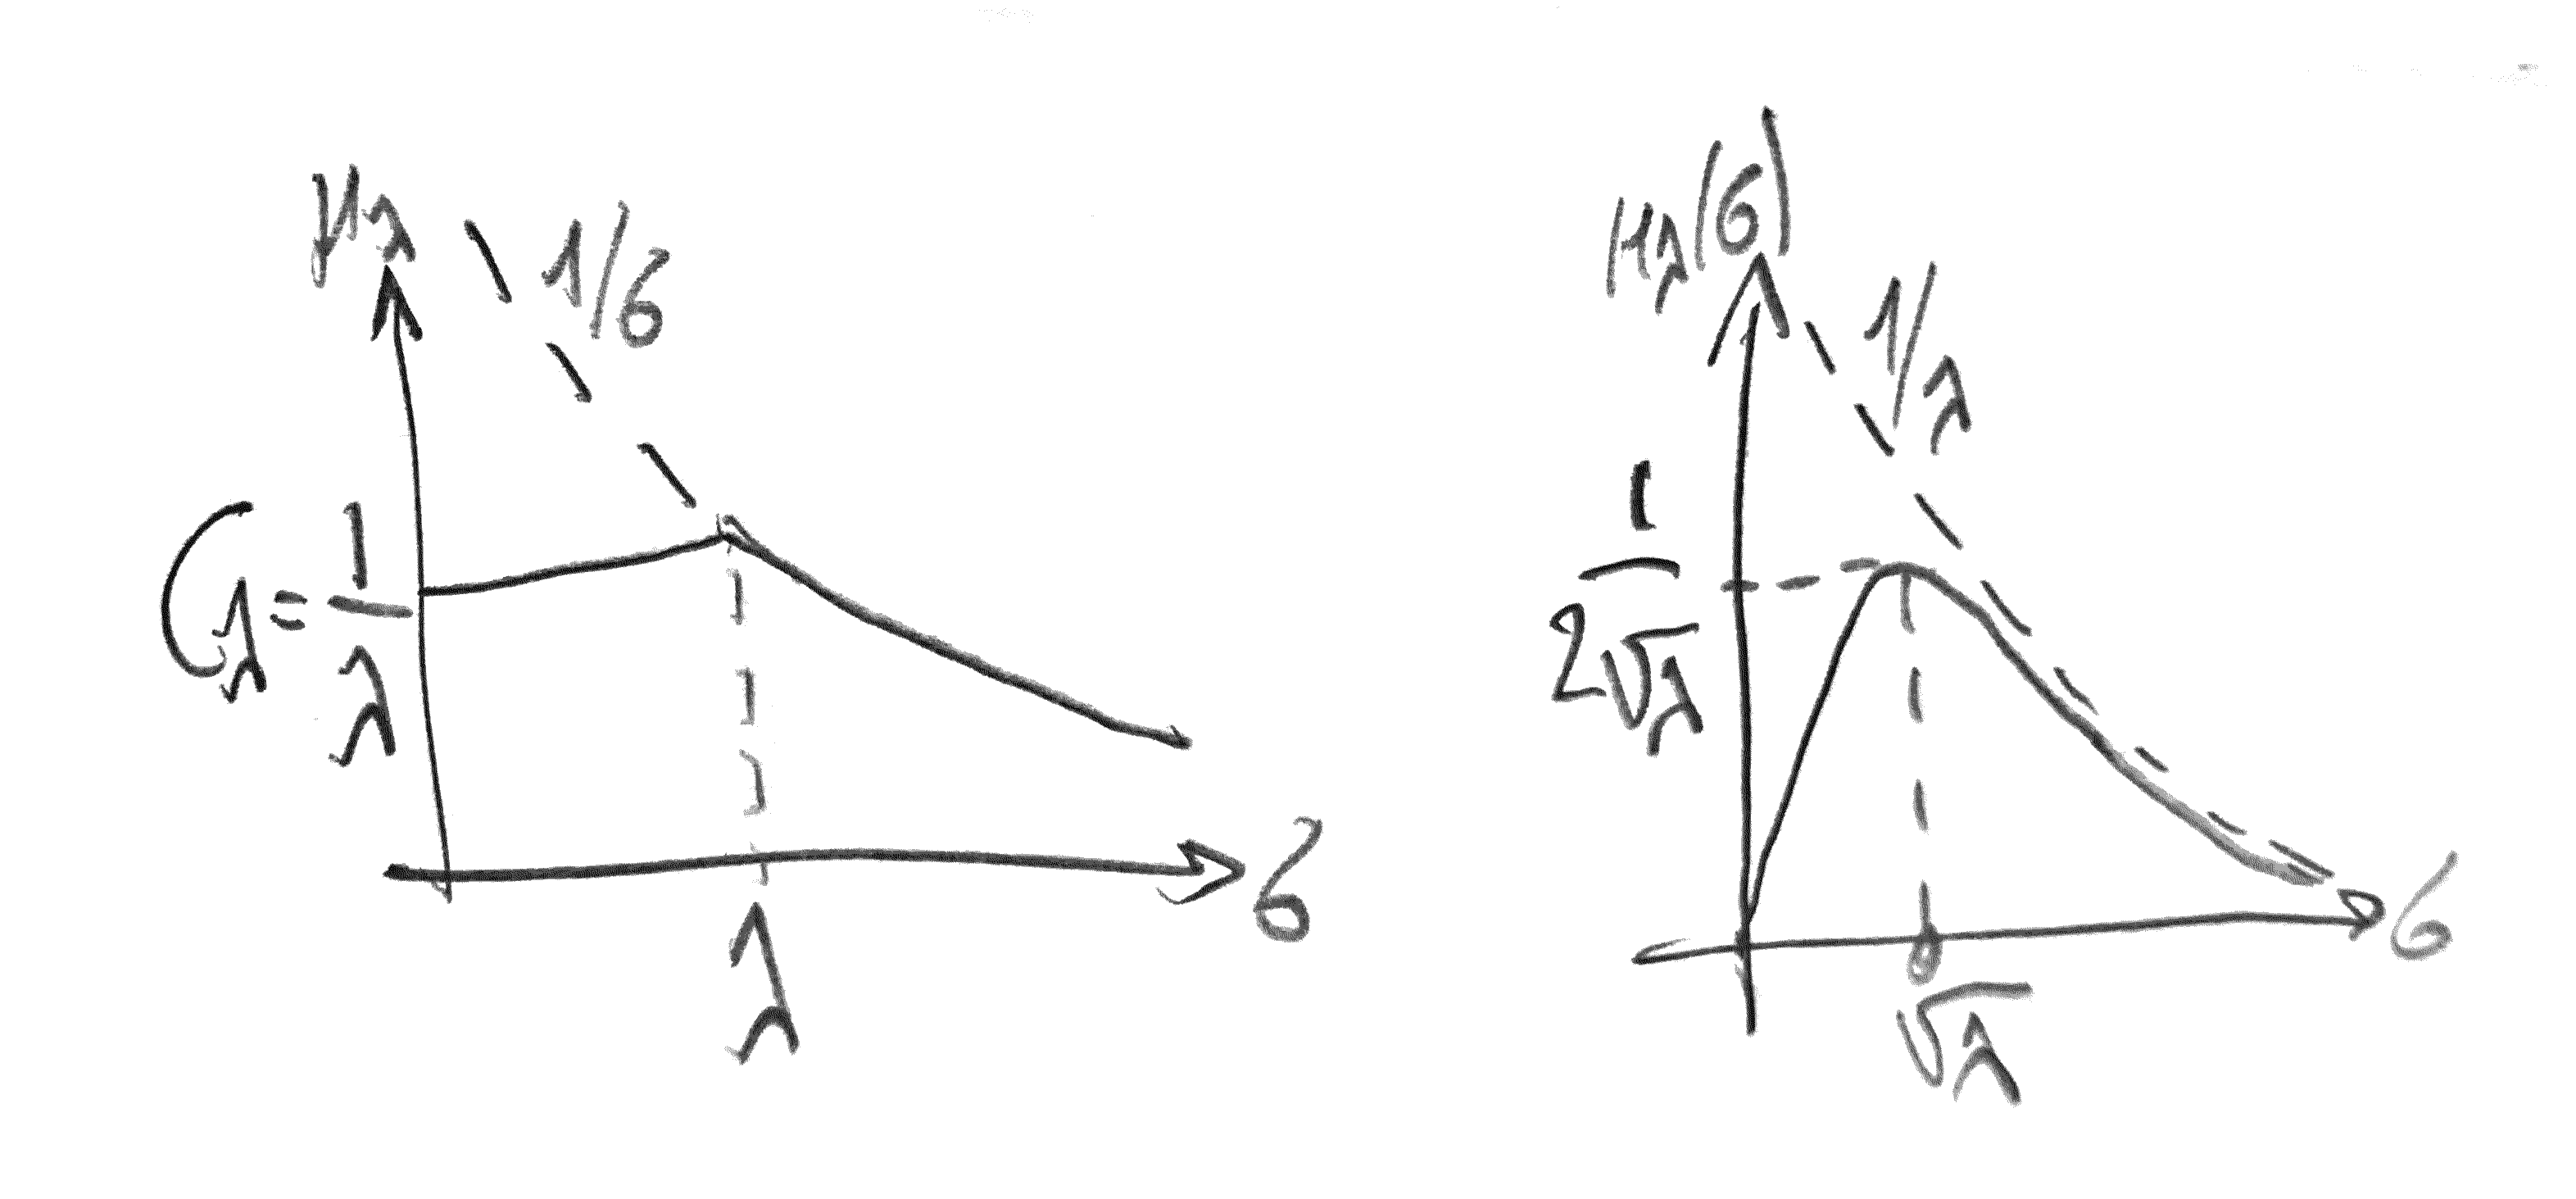
\includegraphics[width=.4\linewidth]{inverse-problems/bound-variance} 
\caption{\label{fig-bound-regul-variance}
Bounding $\mu_{\la}(\si) \leq C_\la = \frac{1}{2\sqrt{\la}}$.
}
\end{figure}


\begin{figure}
\centering
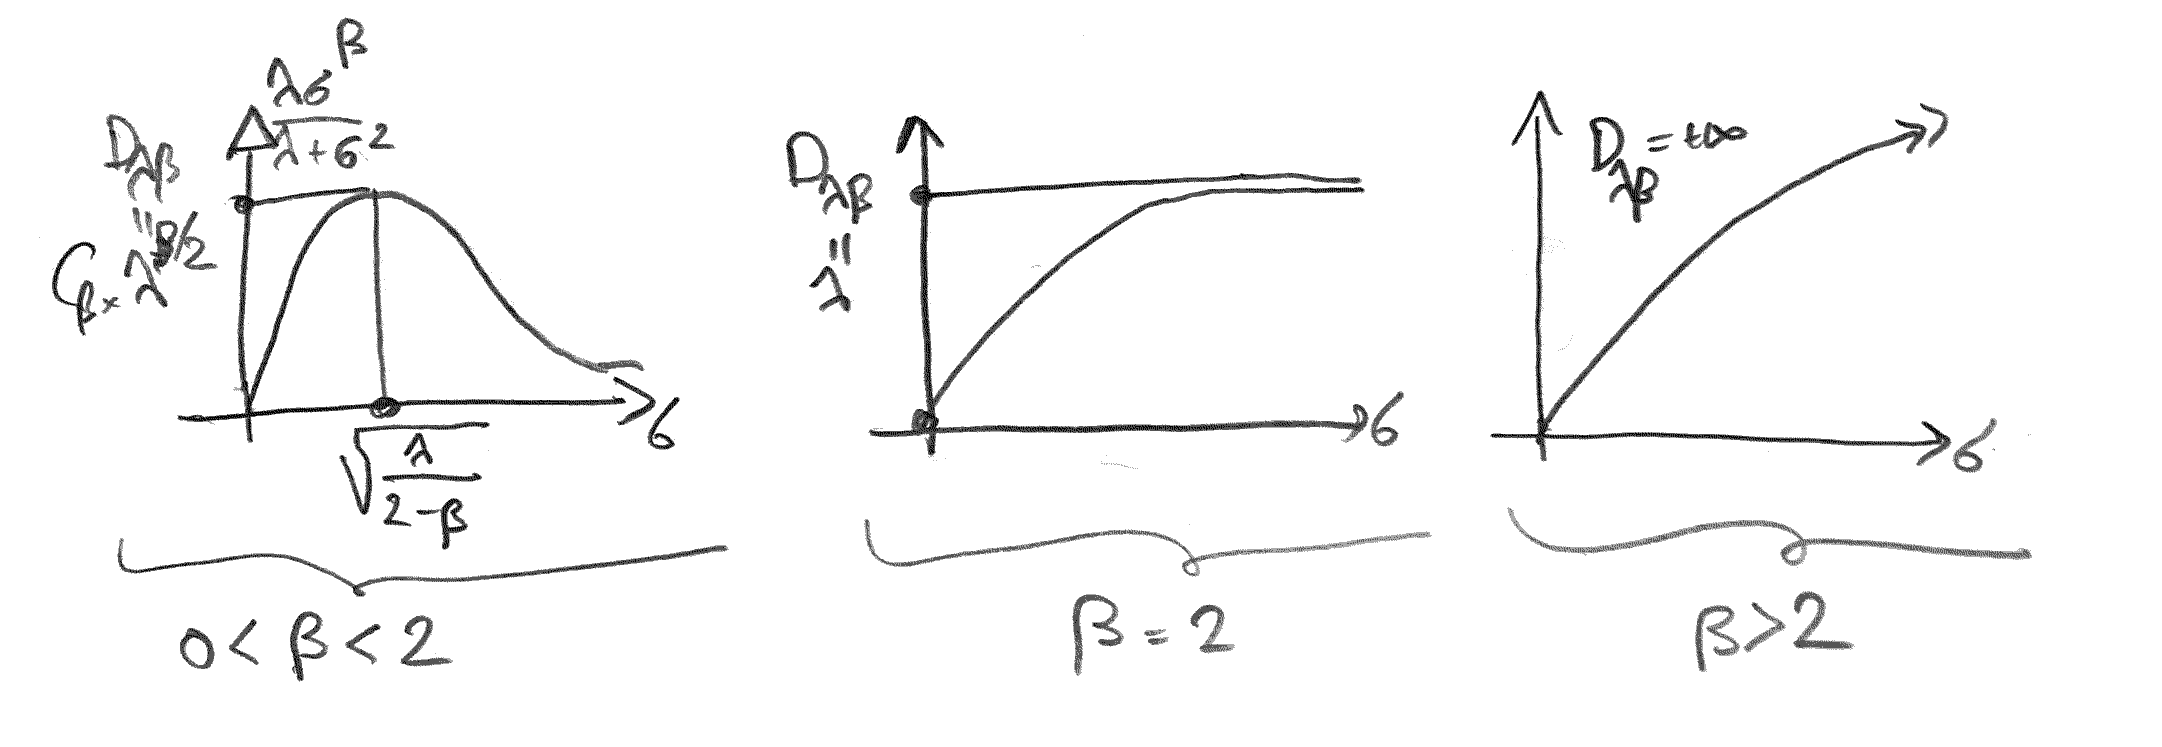
\includegraphics[width=.6\linewidth]{inverse-problems/bound-bias} \quad
\caption{\label{fig-bound-regul}
Bounding $\la \frac{\si^\be}{\la+\si^2} \leq D_{\la,\be}$. 
}
\end{figure}



This theorem shows that using larger $\be \leq 2$ leads to faster convergence rates as $\norm{w}$ drops to zero.
The rate~\eqref{eq-rate-tikhon} however suffers from a ``saturation'' effect, indeed, choosing $\be > 2$ does not helps (it gives the same rate as $\be=2$), and the best possible rate is thus 
\eq{
	\norm{f_\la - f_0} = O( \rho^{\frac{1}{3}} \de^{\frac{2}{3}} ).
}
By choosing more alternative regularization functional $\mu_\la$ and choosing $\be$ large enough, one can show that it is possible to reach rate $\norm{f_\la - f_0} = O( \de^{1-\kappa} )$ for an arbitrary small $\kappa>0$.
%
Figure~\ref{fig-bound-regul-variance} contrast the regularization curve associated to quadratic regularization~\eqref{eq-sol-quad-reg-svd} (right) to the simpler thresholding curve (left) which does not suffers from saturation. Quadratic regularization however is much simpler to implement because it does not need to compute an SVD, is defined using a variational optimization problem and is computable as the solution of a linear system. 
%
One cannot however reach a linear rate $\norm{f_\la - f_0}=O(\norm{w})$. Such rates are achievable using non-linear sparse $\ell^1$ regularizations as detailed in Chapter~\ref{chap-sparse-regul}. 

%%%%%%%%%%%%%%%%%%%%%%%%%%%%%%%%%%%%%%%%%%%%%%%%%%%%%%%%%%%%%%%%
%%%%%%%%%%%%%%%%%%%%%%%%%%%%%%%%%%%%%%%%%%%%%%%%%%%%%%%%%%%%%%%%
%%%%%%%%%%%%%%%%%%%%%%%%%%%%%%%%%%%%%%%%%%%%%%%%%%%%%%%%%%%%%%%%
\section{Quadratic Regularization}

After this theoretical study in infinite dimension, we now turn our attention to more practical matters, and focus only on the finite dimensional setting.

%%%%
\paragraph{Convex regularization.}

Following~\eqref{eq-regul-inv}, the ill-posed problem of recovering an approximation of the high resolution image $f_0 \in \RR^N$ from noisy measures $y = \Phi f_0 + w \in \RR^P$ is regularized by solving a convex optimization problem
\eql{\label{eq-ip-regul}
	f_\la \in  \uargmin{ f \in \RR^N }\; \Ee(f) \eqdef \frac{1}{2} \norm{y-\Phi f}^2 + \la J(f)
}
where $\norm{y-\Phi f}^2$ is the data fitting term (here $\norm{\cdot}$ is the $\ell^2$ norm on $\RR^P$) and $J(f)$ is a convex functional on $\RR^N$.

The Lagrange multiplier $\la$ weights the importance of these two terms, and is in practice difficult to set.
Simulation can be performed on high resolution signal $f_0$ to calibrate the multiplier by minimizing the super-resolution error $\norm{f_0-\tilde f}$, but this is usually difficult to do on real life problems.


In the case where there is no noise, $w = 0$, the Lagrange multiplier $\la$ should be set as small as possible. In the limit where $\la \rightarrow 0$, the unconstrained optimization problem~\eqref{eq-ip-regul} becomes a constrained optimization, as the following proposition explains.
%
Let us stress that, without loss of generality, we can assume that $y \in \Im(\Phi)$, because one has the orthogonal decomposition
\eq{
	\norm{y-\Phi f}^2 = \norm{y-\Proj_{\Im(\Phi)}(y)}^2 + \norm{\Proj_{\Im(\Phi)}(y)-\Phi f}^2
}
so that one can replace $y$ by $\Proj_{\Im(\Phi)}(y)$ in~\eqref{eq-ip-regul}. 

Let us recall that a function $J$ is coercive if
\eq{
	\lim_{\norm{f} \rightarrow +\infty} J(f) = +\infty
}
i.e.
\eq{
	\foralls K, \; \exists R, \norm{x} \geq R \qarrq |J(f)| \geq K.
}
This means that its non-empty levelsets $\enscond{f}{J(f) \leq c}$ are bounded (and hence compact) for all $c$.

\begin{prop}\label{prop-gamma-conv-regul}
We assume that $J$ is coercive and that $y \in \Im(\Phi)$. Then, if for each $\la$, $f_\la$ is a solution of~\eqref{eq-ip-regul}, then $(f_\la)_\la$ is a bounded set and any accumulation point $f^\star$ is a solution of
\eql{\label{eq-ip-regul-noiseless}
	f^\star = \uargmin{f \in \RR^N} \enscond{J(f)}{\Phi f = y}.
}
\end{prop}

\begin{proof}
	Denoting $h$, any solution to~\eqref{eq-ip-regul-noiseless}, which in particular satisfies $\Phi h = y$, because of the optimality condition of $f_\la$ for~\eqref{eq-ip-regul}, one has
	\eq{
		\frac{1}{2\la} \norm{\Phi f_\la-y}^2 + J(f_\la) \leq \frac{1}{2\la} \norm{\Phi h-y}^2 + J(h) = J(h). 
	}
	This shows that $J(f_\la) \leq J(h)$ so that since $J$ is coercive the set $(f_\la)_\la$ is bounded and thus one can consider an accumulation point $f_{\la_k} \rightarrow f^\star$ for $k \rightarrow +\infty$.  Since $\norm{\Phi f_{\la_k}-y}^2 \leq \la_k J(h)$, one has in the limit $\Phi f^\star = y$, so that $f^\star$ satisfies the constraints in~\eqref{eq-ip-regul-noiseless}. Furthermore, by continuity of $J$, passing to the limit in $J(f_{\la_k}) \leq J(h)$, one obtains $J(f^\star) \leq J(h)$ so that $f^\star$ is a solution of~\eqref{eq-ip-regul-noiseless}. 
\end{proof}

Note that it is possible to extend this proposition in the case where $J$ is not necessarily coercive on the full space (for instance the TV functionals in Section~\ref{sec-tv-regul} bellow) but on the orthogonal to $\ker(\Phi)$. The proof is more difficult.


%%%%
\paragraph{Quadratic Regularization.}

The simplest class of prior functional are quadratic, and can be written as
\eql{\label{eq-quad-regul}
	J(f) = \frac{1}{2}\norm{G f}_{\RR^K}^2 = \frac{1}{2} \dotp{L f}{f}_{\RR^N}
}
where $G \in \RR^{K \times N}$ and 
where $L=G^*G \in \RR^{N \times N}$ is a positive semi-definite matrix.
%
The special case~\eqref{eq-regul-normsq} is recovered when setting $G=L=\Id_N$. 

Writing down the first order optimality conditions for~\eqref{eq-ip-regul} leads to
\eq{
	\nabla \Ee(f) = \Phi^*( \Phi f - y ) + \la L f = 0, 
}
hence, if
\eq{
	\ker(\Phi) \cap \ker(G) = \{0\}, 
}
then~\eqref{eq-quad-regul} has a unique minimizer $f_\la$, which is obtained by solving a linear system
\eql{\label{eq-ip-quad-explicit}
	f_\la = ( \Phi^* \Phi + \la L )^{-1} \Phi^* y.  
}
In the special case where $L$ is diagonalized by the singular basis $(v_m)_m$ of $\Phi$, i.e. $L=V \diag(\al_m^2) V^*$, then $f_\la$ reads in this basis 
\eql{\label{eq-sing-diag-ip}
	\dotp{f_{\la}}{v_m} = \frac{\si_m}{\si_m^2 + \la \al_m^2} \dotp{y}{v_m}.
}


%%%
\paragraph{Example of convolution.}

A specific example is for convolution operator 
\eql{\label{eq-convol-example}
	\Phi f = h \star f, 
}
and using $G=\nabla$ be a discretization of the gradient operator, such as for instance using first order finite differences~\eqref{eq-disc-diff-1}. This corresponds to the discrete Sobolev prior introduced in Section~\ref{subsec-disc-priors}.
%
Such an operator compute, for a $d$-dimensional signal $f \in \RR^N$ (for instance a 1-D signal for $d=1$ or an image when $d=2$), an approximation $\nabla f_n \in \RR^d$ of the gradient vector at each sample location $n$. Thus typically, $\nabla : f \mapsto (\nabla f_n)_n \in \RR^{N \times d}$ maps to $d$-dimensional vector fields.
%
Then $-\nabla^* : \RR^{N \times d} \rightarrow \RR^N$ is a discretized divergence operator.
%
In this case, $\De=-GG^*$ is a discretization of the Laplacian, which is itself a convolution operator. One then has
\eql{\label{eq-quad-regul-convol}
	\hat f_{\la,m} = \frac{\hat h_m^* \hat y_m}{|\hat h_m|^2 - \la \hat d_{2,m}}, 
}
where $\hat d_2$ is the Fourier transform of the filter $d_2$ corresponding to the Laplacian. For instance, in dimension 1, using first order finite differences, the expression for $\hat d_{2,m}$ is given in~\eqref{eq-fft-lapl}.




%%%%%%%%%%%%%%%%%%%%%%%%%%%%%%%%%%%%%%%%%%%%%%%%%%%%%%%%%%%%%%%%
\subsection{Solving Linear System}

When $\Phi$ and $L$ do not share the same singular spaces, using~\eqref{eq-sing-diag-ip} is not possible, so that one needs to solve the linear system~\eqref{eq-ip-quad-explicit}, which can be rewritten as
\eq{
	A f = b \qwhereq A \eqdef \Phi^* \Phi + \la L \qandq b = \Phi^* y. 
} 
It is possible to solve exactly this linear system with direct methods for moderate $N$ (up to a few thousands), and the numerical complexity for a generic $A$ is $O(N^3)$. Since the involved matrix $A$ is symmetric, the best option is to use Choleski factorization $A=BB^*$ where $B$ is lower-triangular. In favorable cases, this factorization (possibly with some re-re-ordering of the row and columns) can take advantage of some sparsity in $A$.

For large $N$, such exact resolution is not an option, and should use approximate iterative solvers, which only access $A$ through matrix-vector multiplication. This is especially advantageous for imaging applications, where such multiplications are in general much faster than a naive $O(N^2)$ explicit computation. If the matrix $A$ is highly sparse, this typically necessitates $O(N)$ operations. 
%
In the case where $A$ is symmetric and positive definite (which is the case here), the most well known method is the conjugate gradient methods, which is actually an optimization method solving
\eql{\label{eq-quad-func}
	\umin{f \in \RR^N} \Ee(f) \eqdef \Qq(f) \eqdef \dotp{A f}{f} - \dotp{f}{b}	
}
which is equivalent to the initial minimization~\eqref{eq-ip-regul}. Instead of doing a naive gradient descent (as studied in Section~\ref{sec-grad-descent} bellow), stating from an arbitrary $\itz{f}$, it compute a new iterate $\iit{f}$ from the previous iterates as
\eq{
	\iit{f} \eqdef \uargmin{f} \enscond{ \Ee(f) }{ f \in \it{f} + \Span(\nabla \Ee(\itz{f}), \ldots,\nabla \Ee(f^{\ell}) ) }.
}
The crucial and remarkable fact is that this minimization can be computed in closed form at the cost of two matrix-vector product per iteration, for $k \geq 1$ (posing initially $\itz{d} = \nabla \Ee(\itz{f}) = A\itz{f}-b$)
\eql{\label{eq-iter-cgs}
	\iit{f} = \it{f} - \tau_\ell \it{d}
	\qwhereq	
	\it{d} =  g_\ell + \frac{ \norm{ \it{g} }^2 }{ \norm{g^{(\ell-1)}}^2 } d^{(\ell-1)}
	\qandq
	\tau_\ell = \frac{
			\dotp{ g_\ell }{\it{d}}
		}{ 
			\dotp{A \it{d}}{\it{d}} 
		}			
}
$\it{g} \eqdef \nabla \Ee(\it{f}) = A\it{f}-b$.
%
It can also be shown that the direction $\it{d}$ are orthogonal, so that after $\ell=N$ iterations, the conjugate gradient computes the unique solution $f^{(\ell)}$ of the linear system $A f = b$.  It is however rarely used this way (as an exact solver), and in practice much less than $N$ iterates are computed.
%
It should also be noted that iterations~\eqref{eq-iter-cgs} can be carried over for an arbitrary smooth convex function $\Ee$, and it typically improves over the gradient descent (although in practice quasi-Newton method are often preferred). 



%%%%%%%%%%%%%%%%%%%%%%%%%%%%%%%%%%%%%%%%%%%%%%%%%%%%%%%%%%%%%%%%
%%%%%%%%%%%%%%%%%%%%%%%%%%%%%%%%%%%%%%%%%%%%%%%%%%%%%%%%%%%%%%%%
%%%%%%%%%%%%%%%%%%%%%%%%%%%%%%%%%%%%%%%%%%%%%%%%%%%%%%%%%%%%%%%%
\section{Non-Quadratic Regularization}

%%%%%%%%%%%%%%%%%%%%%%%%%%%%%%%%%%%%%%%%%%%%%%%%%%%%%%%%%%%%%%%%
\subsection{Total Variation Regularization}
\label{sec-tv-regul}

A major issue with quadratic regularization such as~\eqref{eq-quad-regul} is that they typically leads to blurry recovered data $f_\la$, which is thus not a good approximation of $f_0$ when it contains sharp transition such as edges in images. 
%
This is can clearly be seen in the convolutive case~\eqref{eq-quad-regul-convol}, this the restoration operator $\Phi_\la^+ \Phi$ is a filtering, which tends to smooth sharp part of the data.

This phenomena can also be understood because the restored data $f_\la$ always belongs to $\Im(\Phi^*)=\ker(\Phi)^\bot$, and thus cannot contains ``high frequency'' details that are lost in the kernel of $\Phi$. To alleviate this shortcoming, and recover missing information in the kernel, it is thus necessarily to consider non-quadratic and in fact non-smooth regularization. 

%%
\paragraph{Total variation.}

The most well know instance of such a non-quadratic and non-smooth regularization is the total variation prior. For smooth function $f : \RR^d \mapsto \RR$, this amounts to replacing the quadratic Sobolev energy (often called Dirichlet energy) 
\eq{
	\Jsob(f) \eqdef \frac{1}{2} \int_{\RR^d} \norm{\nabla f}_{\RR^d}^2 \d x, 
}
where $\nabla f(x) = (\partial_{x_1} f(x), \ldots, \partial_{x_d} f(x))^\top$ is the gradient, by the (vectorial) $L^1$ norm of the gradient
\eq{
	\Jtv(f) \eqdef \int_{\RR^d} \norm{\nabla f}_{\RR^d} \d x.
}
We refer also to Section~\ref{sec-sob-tv-cont} about these priors.
%
Simply ``removing'' the square $^2$ inside the integral might seems light a small change, but in fact it is a game changer. 

Indeed, while $\Jsob(1_{\Om}) = +\infty$ where $1_{\Om}$ is the indicator a set $\Om$ with finite perimeter $|\Om|<+\infty$, one can show that $\Jtv(1_{\Om})=|\Om|$, if one interpret $\nabla f$ as a distribution $Df$ (actually a vectorial Radon measure) and $\int_{\RR^d} \norm{\nabla f}_{\RR^d} \d x$ is replaced by the total mass $|Df|(\Om)$ of this distribution $m=Df$
\eq{
 	|m|(\Om) = \sup \enscond{\int_{\RR^d}\dotp{h(x)}{\d m(x)}}{ h \in \Cc(\RR^d \mapsto \RR^d),  \foralls x, \norm{h(x)} \leq 1}.
}
The total variation of a function such that $Df$ has a bounded total mass (a so-called bounded variation function) is hence defined as
\eq{
	\Jtv(f) \eqdef \sup \enscond{  \int_{\RR^d} f(x) \diverg(h)(x) \d x  }{ h \in \Cc^1_c(\RR^d;\RR^d), \norm{h}_\infty \leq 1 }.
}
Generalizing the fact that $\Jtv(1_\Om)=|\Om|$, the functional co-area formula reads
\eq{
	\Jtv(f) = \int_\RR \Hh_{d-1}( L_t(f) ) \d t
	\qwhereq
	L_t(f) = \enscond{x}{f(x)=t}
}
and where $\Hh_{d-1}$ is the Hausforf measures of dimension $d-1$, for instance, for $d=2$ if $L$ has finite perimeter $|L|$, then $\Hh_{d-1}(L)=|L|$ is the perimeter of $L$.


%%
\paragraph{Discretized Total variation.}

For discretized data $f \in \RR^N$, one can define a discretized TV semi-norm as detailed in Section~\ref{subsec-disc-priors}, and it reads, generalizing~\eqref{eq-discr-tv} to any dimension
\eq{
	\Jtv(f) = \sum_n \norm{\nabla f_n}_{\RR^d}
}
where $\nabla f_n \in \RR^d$ is a finite difference gradient at location indexed by $n$. 


The discrete total variation prior $\Jtv(f)$ defined in \eqref{eq-discr-tv} is a convex but non differentiable function of $f$, since a term of the form $\norm{\nabla f_n}$ is non differentiable if $\nabla f_n=0$.
%
We defer to chapters~\ref{chap-convex-optim} and~\ref{chap-conv-duality} the study of advanced non-smooth convex optimization technics that allows to handle this kind of functionals.

In order to be able to use simple gradient descent methods, one needs to smooth the TV functional. The general machinery proceeds by replacing the non-smooth $\ell^2$ Euclidean norm $\norm{\cdot}$ by a smoothed version, for instance
\eq{
	\foralls u \in \RR^d, \quad \norm{u}_\epsilon \eqdef \sqrt{ \epsilon^2 + \norm{u} }.
}
This leads to the definition of a smoothed approximate TV functional, already introduced in~\eqref{eq-tv-smoothed}, 
\eq{
	\Jtv^\epsilon(f) \eqdef \sum_n \norm{\nabla f_n}_\epsilon
}
One has the following asymptotics for $\epsilon \rightarrow \{0,+\infty\}$
\eq{
	\norm{u}_\epsilon \overset{\epsilon\rightarrow 0}{\longrightarrow}	\norm{u}
	\qandq
	\norm{u}_\epsilon = \epsilon + \frac{1}{2\epsilon} \norm{u}^2 + O(1/\epsilon^2)
}
which suggest that $\Jtv^\epsilon$ interpolates between $\Jtv$ and $\Jsob$.

The resulting inverse  regularization problem~\eqref{eq-ip-regul} thus reads 
\eql{\label{eq-ip-tv-eps}
	f_\la \eqdef \uargmin{f \in \RR^N} \Ee(f) = \frac{1}{2}\norm{y-\Phi f}^2 + \la \Jtv^\epsilon(f)
}
It is a strictly convex problem (because $\norm{\cdot}_\epsilon$ is strictly convex for $\epsilon>0$) so that its solution $f_\la$ is unique. 



%%%%%%%%%%%%%%%%%%%%%%%%%%%%%%%%%%%%%%%%%%%%%%%%%%%%%%%%%%%%%%%%
\subsection{Gradient Descent Method}
\label{sec-grad-descent}

The optimization program~\eqref{eq-ip-tv-eps} is a example of smooth unconstrained convex optimization of the form
\eql{\label{eq-min-smooth-uncons-ip}
	\umin{f \in \RR^N} \Ee(f)
}
where $\Ee : \RR^N \rightarrow \RR$ is a $\Cc^1$ function. Recall that the gradient $\nabla \Ee : \RR^N \mapsto \RR^N$ of this functional (not to be confound with the discretized gradient $\nabla f \in \RR^N$ of $f$) is defined by the following first order relation
\eq{
	\Ee(f+r) = \Ee(f) + \dotp{f}{r}_{\RR^N} + O(\norm{r}_{\RR^N}^2)
}
where we used $O(\norm{r}_{\RR^N}^2)$ in place of $o(\norm{r}_{\RR^N})$ (for differentiable function) because we assume here $\Ee$ is of class $\Cc^1$ (i.e. the gradient is continuous). 

For such a function, the gradient descent algorithm is defined as
\eql{\label{eq-grad-desc}
	\iit{f} \eqdef \it{f} - \tau_\ell \nabla \Ee( \it{f} ), 
}
where the step size $\tau_\ell>0$ should be small enough to guarantee convergence, but large enough for this algorithm to be fast.

We refer to Section~\ref{sec-grad-descent} for a detailed analysis of the convergence of the gradient descent, and a study of the influence of the step size $\tau_\ell$.



%%%%%%%%%%%%%%%%%%%%%%%%%
\subsection{Examples of Gradient Computation}
\label{eq-example-grad}

Note that the gradient of a quadratic function $\Qq(f)$ of the form~\eqref{eq-quad-func} reads
\eq{
	\nabla \Gg(f) = Af-b.
}
In particular, one retrieves that the first order optimality condition $\nabla \Gg(f)=0$ is equivalent to the linear system $Af=b$. 

For the quadratic fidelity term $\Gg(f)=\frac{1}{2}\norm{\Phi f-y}^2$, one thus obtains
\eq{
	\nabla \Gg(f) = \Phi^*(\Phi y - y). 
}

In the special case of the regularized TV problem~\eqref{eq-ip-tv-eps}, the gradient of $\Ee$ reads
\eq{
	\nabla \Ee(f) = \Phi^*(\Phi y - y) + \la \nabla \Jtv^\epsilon(f).
}
Recall the chain rule for differential reads $\partial (\Gg_1 \circ \Gg_2) = \partial \Gg_1 \circ \partial \Gg_2$, but that gradient vectors are actually transposed of differentials, so that for $\Ee = \Ff \circ \Hh$ where $\Ff : \RR^P \rightarrow \RR$ and $\Hh : \RR^N \rightarrow \RR^P$, one has
\eq{
	\nabla \Ee(f) = [ \partial \Hh( f ) ]^*\pa{ \nabla \Ff( \Hh f ) }.
}

Since $\Jtv^\epsilon = \norm{\cdot}_{1,\epsilon} \circ \nabla$, one thus has
\eq{
	\nabla \Jtv^\epsilon = \nabla^\star \circ ( \partial \norm{\cdot}_{1,\epsilon} )
	\qwhereq
	\norm{u}_{1,\epsilon} = \sum_n \norm{u_n}_\epsilon
}
so that 
\eq{
	\Jtv^\epsilon(f) = -\diverg( \Nn^\epsilon( \nabla f) ), 
}
where $\Nn^\epsilon(u) = ( u_n/\norm{u_n}_\epsilon )_n$ is the smoothed-normalization operator of vector fields (the differential of $\norm{\cdot}_{1,\epsilon}$), and where $\diverg=-\nabla^*$ is minus the adjoint of the gradient.

Since $\diverg=-\nabla^*$, their Lipschitz constants are equal $\norm{\diverg}_\text{op}=\norm{\nabla}_\text{op}$, and is for instance equal to $\sqrt{2d}$ for the discretized gradient operator. 
%
Computation shows that the Hessian of $\norm{\cdot}_\epsilon$ is bounded by $1/\epsilon$, so that for the smoothed-TV functional, the Lipschitz constant of the gradient is upper-bounded by
\eq{
	L = \frac{\norm{\nabla}^2}{\epsilon} + \norm{\Phi}_{\text{op}}^2.
}
Furthermore, this functional is strongly convex because $\norm{\cdot}_\epsilon$ is $\epsilon$-strongly convex, and the Hessian is lower bounded by
\eq{
	\mu = \epsilon + \si_{\min}( \Phi )^2
}
where $\si_{\min}( \Phi )$ is the smallest singular value of $\Phi$. For ill-posed problems, typically $\si_{\min}( \Phi )=0$ or is very small, so that both $L$ and $\mu$ degrades (tends respectively to $0$ and $+\infty$) as $\epsilon \rightarrow 0$, so that gradient descent becomes prohibitive for small $\epsilon$, and it is thus required to use dedicated non-smooth optimization methods detailed in the following chapters. 
%
On the good news side, note however that in many case, using a small but non-zero value for $\epsilon$ often leads to better a visually more pleasing results, since it introduce a small blurring which diminishes the artifacts (and in particular the so-called ``stair-casing'' effect) of TV regularization. 



%%%%%%%%%%%%%%%%%%%%%%%%%%%%%%%%%%%%%%%%%%%%%%%%%%%%%%%%%%%%%%%%
%%%%%%%%%%%%%%%%%%%%%%%%%%%%%%%%%%%%%%%%%%%%%%%%%%%%%%%%%%%%%%%%
%%%%%%%%%%%%%%%%%%%%%%%%%%%%%%%%%%%%%%%%%%%%%%%%%%%%%%%%%%%%%%%%
\section{Examples of Inverse Problems}

We detail here some inverse problem in imaging that can be solved using quadratic regularization or non-linear TV.

%%%%%%%%%%%%%%%%%%%%%%%%%%%%%%%%%%%%%%%%%%%%%%%%%%%%%%%%%%%%%%%%
\subsection{Deconvolution}
\label{subsec-deconv}

The blurring operator \eqref{eq-deblurring-operator} is diagonal over Fourier, so that quadratic regularization are easily solved using Fast Fourier Transforms when considering periodic boundary conditions. We refer to~\eqref{eq-convol-example} and the correspond explanations. TV regularization in contrast cannot be solved with fast Fourier technics, and is thus much slower.


%%%%%%%%%%%%%%%%%%%%%%%%%%%%%%%%%%%%%%%%%%%%%%%%%%%%%%%%%%%%%%%%
\subsection{Inpainting}
\label{sec-inpainting-variational}

For the inpainting problem, the operator defined in \eqref{eq-inp-operator} is diagonal in space
\eq{
	 \Phi = \diag_m( \de_{\Om^c}[m] ),
}
and is an orthogonal projector $\Phi^* = \Phi$.

In the noiseless case, to constrain the solution to lie in the affine space $\enscond{f \in \RR^N}{y=\Phi f}$, we use the orthogonal projector
\eq{
	\foralls x, \quad P_y(f)(x) = \choice{
		f(x) \qifq x \in \Om,\\
		\; y(x) \quad \qifq x \notin \Om.
	}
}


In the noiseless case, the recovery \eqref{eq-ip-regul-noiseless} is solved using a projected gradient descent.
For the Sobolev energy, the algorithm iterates
\eq{
	\iit{f}= P_y( \it{f} + \tau \Delta \it{f} ).
}
which converges if $\tau < 2 / \norm{\Delta} = 1/4$. Figure \ref{fig-inp-sob-iter} shows some iteration of this algorithm, which progressively interpolate within the missing area. 

% Table \ref{inverse-inpainting-sob} details the implementation of the inpainting with the Sobolev prior.

%\matlab{matlab/inverse-inpainting-sob.m
%}{
%Inpainting with Sobolev regularization. The mask $\Om$ is given in \matvar{mask}, so that the masked indices are \matvar{f(mask)}, the observations in \matvar{y}. The solution is given in \matvar{fsob}.
%}{inverse-inpainting-sob}

\myfigure{
\tabquatre{
\image{invpbm}{.24}{sob-inp-iter-1}&
\image{invpbm}{.24}{sob-inp-iter-2}&
\image{invpbm}{.24}{sob-inp-iter-3}&
\image{invpbm}{.24}{sob-inp-iter-4} \\
$k=1$ & $k=10$ & $k=20$ & $k=100$ 
}
}{%
	Sobolev projected gradient descent algorithm. %	
}{fig-inp-sob-iter}

%\myfigure{
%\tabdeux{
%\image{invpbm}{.3}{sob-inp-decay-conv}&
%\image{invpbm}{.3}{sob-inp-decay-energy} \\
%$\log_{10}( E(\it{f})/E(f^\star)-1 )$ &
%$\log_{10}( \norm{\it{f}-f^\star}/\norm{f_0} )$
%}
%}{%
%	Decay of the energy and convergence for Sobolev inpainting.%	
%}{fig-sob-inp-decay}

Figure \ref{fig-inpainting-parrot} shows an example of Sobolev inpainting to achieve a special effect.

\myfigure{
\tabtrois{
\image{invpbm}{.3}{inpainting-parrot-image}&
\image{invpbm}{.3}{inpainting-parrot-mask}&
\image{invpbm}{.3}{inpainting-parrot-sobolev}\\
Image $f_0$ & Observation $y=\Phi f_0$ & Sobolev $f^\star$ \\
}
}{%
	Inpainting the parrot cage. %	
}{fig-inpainting-parrot}

For the smoothed TV prior, the gradient descent reads
\eq{
	\iit{f}= P_y\pa{
			\it{f} + \tau \diverg\pa{ \frac{ \nabla \it{f}}{ \sqrt{\epsilon^2+\norm{\nabla \it{f}}^2} } }
		}
}
which converges if $\tau < \epsilon/4$.

Figure \ref{fig-inpainting-cameraman} compare the Sobolev inpainting and the TV inpainting for a small value of $\epsilon$. The SNR is not improved by the total variation, but the result looks visually slightly better.

% For special effects : $\Ldeux$ error and SNR are not good measures of quality, $f^\star$ is very different from $f_0$ ! Pereceptual metric, visual inspection.

\myfigure{
\tabdeux{
\image{invpbm}{.3}{inpainting-cameraman-image}&
\image{invpbm}{.3}{inpainting-cameraman-observations}\\
Image $f_0$ & Observation $y=\Phi f_0$ \\
\image{invpbm}{.3}{inpainting-cameraman-sobolev}&
\image{invpbm}{.3}{inpainting-cameraman-tv} \\
Sobolev $f^\star$ & TV $f^\star$ \\
SNR=?dB & SNR=?dB 
}
}{%
	Inpainting with Sobolev and TV regularization. %	
}{fig-inpainting-cameraman}



%%%%%%%%%%%%%%%%%%%%%%%%%%%%%%%%%%%%%%%%%%%%%%%%%%%%%%%%%%%%%%%%
\subsection{Tomography Inversion}

In medical imaging, a scanner device compute projection of the human body along rays $\De_{t,\th}$ defined
\eq{
	x \cdot \tau_\theta = x_1 \cos\th + x_2\sin\th = t
}
where we restrict ourself to 2D projection to simplify the exposition.

The scanning process computes a Radon transform, which compute the integral of the function to acquires along rays
\eq{
	\foralls \th \in [0,\pi), \foralls t \in \RR, \quad
	p_{\th}(t) = \int_{\De_{t,\th}} f(x) \,d s
	 = \iint f(x)\, \de( x \cdot \tau_\theta - t )\, d x 
}
see Figure \eqref{fig-tomo-principle}

\myfigure{
\image{invpbm}{.4}{tomo-principle}
}{%
	Principle of tomography acquisition. %	
}{fig-tomo-principle}

The Fourier slice theorem relates the Fourier transform of the scanned data to the 1D Fourier transform of the data along rays
\eql{\label{eq-fourier-slice}
	\foralls \th \in [0,\pi)~,~ 
\foralls \xi \in \RR\quad
		\hat p_\th(\xi) = \hat f( \xi \cos \th, \xi \sin \th ).
}
This shows that the pseudo inverse of the Radon transform is computed easily over the Fourier domain using inverse 2D Fourier transform
\eq{
	f(x) = 
\frac{1}{2\pi} \int_{0}^\pi p_\th \star h(x \cdot \tau_\theta)\, d \th
}
with $\hat h(\xi) = |\xi|$.


\myfigure{
\tabtrois{
% \image{invpbm}{.4}{tomo-radon}
\image{invpbm}{.3}{tomo-image}&
\image{invpbm}{.35}{tomo-radon-subsample}&
\image{invpbm}{.3}{tomo-radon-fourier}\\
Image $f$ & Radon sub-sampling & Fourier domain
}
}{%
	Partial Fourier measures. %	
}{fig-tomo-radon-subsample}


Imaging devices only capture a limited number of equispaced rays at orientations $\{ \th_k = \pi/k \}_{0 \leq k < K}$. This defines a tomography operator which corresponds to a partial Radon transform
\eq{
	R f = ( p_{\th_k} )_{0 \leq k < K}.
}
Relation \eqref{eq-fourier-slice} shows that knowing $R f$ is equivalent to knowing the Fourier transform of $f$ along rays, 
\eq{
	\{ \hat f(\xi \cos(\th_k), \xi \sin(\th_k)) \}_k.
}
We thus simply the acquisition process over the discrete domain and model it as computing directly samples of the Fourier transform 
\eq{
	\Phi f = ( \hat f[\om] )_{\om \in \Om} \in \RR^P
}
where $\Om$ is a discrete set of radial lines in the Fourier plane, see Figure \ref{fig-tomo-radon-subsample}, right.

In this discrete setting, recovering from Tomography measures $y=R f_0$ is equivalent in this setup to inpaint missing Fourier frequencies, and we consider partial noisy Fourier measures
\eq{
	\foralls \om \in \Om, \quad y[\om] = \hat f[\om] + w[\om]
}
where $w[\om]$ is some measurement noise, assumed here to be Gaussian white noise for simplicity.

\myfigure{
\tabtrois{
\image{invpbm}{.3}{tomo-image}&
\image{invpbm}{.3}{tomo-pinv-13}&
\image{invpbm}{.3}{tomo-pinv-32}\\
Image $f_0$ & 13 projections & 32 projections.
}
}{%
	Pseudo inverse reconstruction from partial Radon projections. %	
}{fig-tomo-pinv}

The peuso-inverse $f^+ = R^+ y$ defined in \eqref{eq-pseudo-inverse} of this partial Fourier measurements  reads 
\eq{
	{\hat f}^+[\om] = \choice{
		y[\om] \qifq \om \in \Om,\\
		\; 0 \qifq \om \notin \Om.
	}
}
Figure \ref{fig-tomo-pinv} shows examples of pseudo inverse reconstruction for increasing size of $\Om$. This reconstruction exhibit serious artifact because of bad handling of Fourier frequencies (zero padding of missing frequencies).

The total variation regularization \eqref{eq-tv-dn} reads
\eq{
	f^\star \in \uargmin{f} \frac{1}{2}\sum_{\om \in \Om} |y[\om] - \hat f[\om]|^2 
	+ \la \normTV{f}.
}
It is especially suitable for medical imaging where organ of the body are of relatively constant gray value, thus resembling to the cartoon image model introduced in Section \ref{subsec-cartoon-images}. Figure \ref{fig-tomo-tv} compares this total variation recovery to the pseudo-inverse for a synthetic cartoon image. This shows the hability of the total variation to recover sharp features when inpainting Fourier measures. This should be contrasted with the difficulties that faces TV regularization to inpaint over the spacial domain, as shown in Figure \ref{fig-inpainting-lena}.

\myfigure{
\tabtrois{
\image{invpbm}{.3}{tomo-image}&
\image{invpbm}{.3}{tomo-pinv-fourier}&
\image{invpbm}{.3}{tomo-tv}\\
Image $f_0$ & Pseudo-inverse & TV
}
}{%
	Total variation tomography inversion. %	
}{fig-tomo-tv}

% !TEX root = ../FundationsDataScience.tex

\chapter{Sparse Regularization}
\label{chap-sparse-regul}

Ref \cite{mallat2008wavelet,starck2015sparse,scherzer2009variational}


%%%%%%%%%%%%%%%%%%%%%%%%%%%%%%%%%%%%%%%%%%%%%%%%%%%%%%%%%%%%%%%%%%%%%%
%%%%%%%%%%%%%%%%%%%%%%%%%%%%%%%%%%%%%%%%%%%%%%%%%%%%%%%%%%%%%%%%%%%%%%
%%%%%%%%%%%%%%%%%%%%%%%%%%%%%%%%%%%%%%%%%%%%%%%%%%%%%%%%%%%%%%%%%%%%%%
\section{Sparsity Priors}

%%%%%%%%%%%%%%%%%%%%%%%%%%%%%%%%%%%%%%%%%%%%%%%%%%%%%%%%%%%%%%%%%%%%%%
\subsection{Ideal sparsity prior.}

As detailed in Chapter \ref{chap-approximation}, it is possible to use an orthogonal basis $\Bb = \{ \psi_m \}_m$ to efficiently approximate an image $f$ in a given class $f \in \Th$ with a few atoms from $\Bb$. 

To measure the complexity of an approximation with $\Bb$, we consider the $\lzero$ prior, which counts the number of non-zero coefficients in $\Bb$
\eq{
	\Jz(f) \eqdef \#\enscond{m}{\dotp{f}{\psi_m} \neq 0}
	\qwhereq
	x_m = \dotp{f}{\psi_m}.
}
One often also denote it as the $\lzero$ ``pseudo-norm''
\eq{
	\normz{x} \eqdef \Jz(f).
}
which we treat here as an ideal sparsity measure for the coefficients $x$ of $f$ in $\Bb$.

Natural images are not exactly composed of a few atoms, but they can be well approximated by a function $f_M$ with a small ideal sparsity $M=\Jz(f)$. In particular, the best $M$-term approximation defined in \eqref{eq-nonlinear-approx} is defined by
\eq{
	f_M = \sum_{ |\dotp{f}{\psi_m}|>T } \dotp{f}{\psi_m} \psi_m
	\qwhereq
	M = \#\enscond{m}{|\dotp{f}{\psi_m}|>T}.
}
As detailed in Section \ref{sec-signal-models}, discontinuous images with bounded variation have a fast decay of the approximation error $\norm{f-f_M}$. Natural images $f$ are well approximated by images with a small value of the ideal sparsity prior $\Jz$.

Figure \ref{fig-sparsity-wav} shows an examples of decomposition of a natural image in a wavelet basis, $\psi_m = \psi_{j,n}^\om$ $m=(j,n,\om)$. This shows that most $\dotp{f}{\psi_m}$ are small, and hence the decomposition is quite sparse.

\myfigure{
\tabdeux{
\image{variational}{.3}{sparsity-image}&
\image{variational}{.3}{sparsity-wav}\\
Image $f$ & Coefficients $\dotp{f}{\psi_m}$
}
}{%
	Wavelet coefficients of natural images are relatively sparse.
}{fig-sparsity-wav}


%%%%%%%%%%%%%%%%%%%%%%%%%%%%%%%%%%%%%%%%%%%%%%%%%%%%%%%%%%%%%%%%%%%%%%
\subsection{Convex relaxation}

Unfortunately, the ideal sparsity prior $\Jz$ is difficult to handle numerically because $\Jz(f)$ is not a convex function of $f$. For instance, if $f$ and $g$ have non-intersecting supports of there coefficients in $\Bb$, then $\Jz( (f+g)/2 ) = \Jz(f)+\Jz(g)$, which shows the highly non-convex behavior of $\Jz$.

This ideal sparsity $\Jz$ is thus not amenable to minimization, which is an issue to solve general inverse problems considered in Section \ref{chap-invpbm}. 

We consider a family of $\ell^q$ priors for $q>0$, intended to approximate the ideal prior $\Jz$ 
\eq{
	J_q(f) = \displaystyle \sum_m |\dotp{f}{\psi_m}|^q.
}
As shown in Figure \ref{fig-sparsity-lq}, the unit balls in $\RR^2$ associated to these priors are shrinking toward the axes, which corresponds to the unit ball for the $\lzero$ pseudo norm. In some sense, the $J_q$ priors are becoming closer to $\Jz$ as $q$ tends to zero, and thus $J_q$ favors sparsity for small $q$.


\myfigure{
\image{variational}{1}{sparsity-lq-balls}
}{%
	$\ell^q$ balls $\enscond{x}{J_q(x) \leq 1}$ for varying $q$.
}{fig-sparsity-lq}


The prior $J_q$ is convex if and only if $q \geq 1$. To reach the highest degree of sparsity while using a convex prior, we consider the $\lun$ sparsity prior $\Ju$, which is thus defined as 
\eql{\label{eq-dfn-lun-prior}
	\Ju(f) = \norm{(\dotp{f}{\psi_m})}_1 = \sum_m |\dotp{f}{\psi_m}|.
}
In the following, we consider discrete orthogonal bases $\Bb = \{\psi_m\}_{m=0}^{N-1}$ of $\RR^N$.


%%%%%%%%%%%%%%%%%%%%%%%%%%%%%%%%%%%%%%%%%%%%%%%%%%%%%%%%%%%%%%%%%%%%%%
\subsection{Sparse Regularization and Thresholding}

Given some orthogonal basis $\{\psi_m\}_m$ of $\RR^N$, the denoising by regularization \eqref{eq-regul-denoising} is written using the sparsity $\Jz$ and $\Ju$ as 
\eq{
	f^\star = \uargmin{g \in \RR^N} \frac{1}{2} \norm{f-g}^2 + \la J_q(f)
}
for $q=0$ or $q=1$. It can be re-written in the orthogonal basis as
\eq{
	f^\star = \sum_m x^\star_m \psi_m
}
\eq{
	\qwhereq
	x^{\star} = \uargmin{y \in \RR^N} \sum_m \frac{1}{2} |x_m-y_m|^2 + \la |y_m|^q
}
where $x_m \eqdef \dotp{f}{\psi_m}$, $y_m \eqdef \dotp{g}{\psi_m}$, and where we use the following slight abuse of notation for $q=0$
\eq{
	\foralls u \in \RR, \quad
	|u|^0=
	\choice{
		0 \qifq u=0, \\ 1 \quad \text{otherwise.} 
	}
}
Each coefficients of the denoised image is the solution of a 1-D optimization problem
\eql{\label{eq-var-1D-spars}
	x_m^\star = \uargmin{u \in \RR}  \frac{1}{2} |x_m-u|^2 + \la |u|^q
}
and the following proposition this optimization is solved exactly in closed form using thresholding.

\begin{prop}\label{prop-equiv-sparse-thresh}
One has
\eql{\label{eq-equiv-sparse-thresh}
	x^{\star}_m = S_T^q( x_m )
	\qwhereq 
	\choice{
		T = \sqrt{2 \la} \qforq q=0,\\
		T = \la \qforq q=1,
	}
}
where 
\eql{\label{eq-hard-thresh}
	\foralls u \in \RR, \quad
	S_T^0(u) \eqdef
	\choice{
		0 \qifq |u| < T, \\
		u \quad\text{otherwise}	
	}
} 
is the hard thresholding introduced in~\eqref{eq-hard-thresh-denoise}, and 
\eql{\label{eq-soft-thresh}
	\foralls u \in \RR, \quad
	S_T^1(u) \eqdef  \sign(u) ( |u|-T )_+
} 
is the soft thresholding introduced in~\eqref{eq-soft-thresh-denoise}.
\end{prop}

	
\begin{proof}
	One needs to solve~\eqref{eq-var-1D-spars}. Figure~\ref{fig-varspars}, left shows the function $\norm{x-y}^2+T^2 \norm{x}_0$, and the minimum is clearly at $x=0$ when $T \geq y$, and at $x=y$ otherwise. This is thus a hard thresholding with threshold $T^2=2\la$. 
	%
	Figure~\eqref{fig-varspars}, right, shows the evolution with $\la$ of the function $\frac{1}{2}\norm{x-y}^2+\la |x|$. 
	% 
	For $x>0$, one has $F'(x)=x-y+\la$ wich is $0$ at $x=y-\la$.
	The minimum is at $x=y-\la$ for $\la \leq y$, and stays at $0$ for all $\la>y$. 
\end{proof}

\myfigure{
\image{sparse-reg}{.19}{var-l0}
%
\image{sparse-reg}{.19}{var-l1-1}
\image{sparse-reg}{.19}{var-l1-2}
\image{sparse-reg}{.19}{var-l1-3}
\image{sparse-reg}{.19}{var-l1-4}
}{%	
	Leftmost: function $\norm{\cdot-y}^2+T^2 \norm{\cdot}_0$ .
	%
	Others: evolution with $\la$ of the function $F(x) \eqdef \frac{1}{2}\norm{\cdot-y}^2+\la |\cdot|$. %	
}{fig-varspars}




One thus has
\eq{
	f_{\la,q} = \sum_m S_T^q( \dotp{f}{\psi_m} ) \psi_m.
}
As detailed in Section \ref{sec-nl-denoising-thresh}, these denoising methods has the advantage that the threshold is simple to set for Gaussian white noise $w$ of variance $\si^2$. Theoretical values indicated that $T = \sqrt{2\log(N)} \si$ is asymptotically optimal, see Section \ref{subsec-minimax-denoise}. In practice, one should choose $T \approx 3\si$ for hard thresholding ($\lzero$ regularization), and $T \approx 3\si/2$ for soft thresholding ($\lun$ regularization), see Figure \ref{fig-wavthresh-2d}.



% Bayesian interpretation:  $\dotp{f}{\psi_m}$ i.i.d. $ \sim$ generalized Gaussian


%%%%%%%%%%%%%%%%%%%%%%%%%%%%%%%%%%%%%%%%%%%%%%%%%%%%%%%%%%%%%%%%
%%%%%%%%%%%%%%%%%%%%%%%%%%%%%%%%%%%%%%%%%%%%%%%%%%%%%%%%%%%%%%%%
%%%%%%%%%%%%%%%%%%%%%%%%%%%%%%%%%%%%%%%%%%%%%%%%%%%%%%%%%%%%%%%%
\section{Sparse Regularization of Inverse Problems}
\label{sec-sparse-ip}

Sparse $\lun$ regularization in an orthogonal basis $\{\psi_m\}_m$ of $\RR^N$ makes use of the $\Ju$ prior defined in \eqref{eq-dfn-lun-prior}, so that the inversion is obtained by solving the following convex program
\eql{\label{eq-bpdn}
	f_\la \in \uargmin{f \in \RR^N} \frac{1}{2}\norm{y-\Phi f}^2 + \la \sum_m |\dotp{f}{\psi_m}|.
}
This corresponds to the basis pursuit denoising for sparse approximation introduced by Chen, Donoho and Saunders in \cite{chen-basis-pursuit}. The resolution of \eqref{eq-bpdn} can be perform using an iterative thresholding algorithm as detailed in Section \ref{subsec-proximal-ip}. 

%%%
\paragraph{Analysis vs. synthesis priors.}

When the set of atoms $\Psi = \{\psi_m\}_{m=1}^Q$ is non-orthognal (and might even be redundant in the case $Q>N$), there is two distincts way to generalizes problem~\eqref{eq-bpdn}, which we formulate as in~\eqref{}, by introducing a generic convex prior $J$
\eql{\label{eq-regul-generic}
	f_\la \in \uargmin{f \in \RR^N} \frac{1}{2}\norm{y-\Phi f}^2 + \la J(f).
}
In the following, with a slight abuse of notation, we denote the ``analysis'' and ``synthesis'' operator as
\eq{
	\Psi : x \in \RR^Q \mapsto \Psi x = \sum_m x_m \psi_m
	\qandq
	\Psi^* : f \in \RR^N \mapsto ( \dotp{f}{\psi_m} )_{m=1}^Q \in \RR^Q.
}

The so-called analysis-type prior is simply measuring the sparsity of the correlations with the atoms in the dictionary
\eql{\label{eq-sparsity-analysis}
	J_1^{\text{A}}(f) \eqdef \sum_m |\dotp{f}{\psi_m}| = \norm{\Psi^* f}_1.
}
The so-called synthesis-type priori in contrast measure the sparsity of the sparsest expansion of $f$ in $\Psi$, i.e.
\eql{\label{eq-sparsity-synthesis}
	J_1^{\text{S}}(f) \eqdef \umin{x \in \RR^q, \Psi x = f} \norm{x}_1.  
}
While the analysis regularization~\eqref{eq-sparsity-analysis} seems simpler to handle, it is actually the contrary. Solving~\eqref{eq-regul-generic} with $J=J_1^{\text{A}}$ is in fact quite involved, and necessitate typically primal-dual algorithm as detailed in Chapter~\ref{chap-conv-duality}. Furthermore, the theoretical study of the performance of the resulting regularization method is mostly an open problem. 

We thus now focus on the synthesis regularization problem $J=J_1^{\text{S}}$, and we re-write~\eqref{eq-regul-generic} conveniently as $f_\la = \Psi x_\la$ where $x_\la$ is any solution of the following Basis Pursuit Denoising problem
\eql{\label{eq-lasso-lagr-ip}
	x_\la \in \uargmin{x \in \RR^Q} \frac{1}{2\la} \norm{y-Ax}^2 + \norm{x}_1
} 
where we introduced the following matrix
\eq{
	A \eqdef \Phi \Psi \in \RR^{P \times Q}. 
}
As $\la \rightarrow 0$, we consider the following limit constrained problem
\eql{\label{eq-lasso-constr-ip}
	x^\star = \uargmin{A x = y} \norm{x}_1
} 
and the signal is recovered as $f^\star=\Psi x^\star \in \RR^N$.


% This can be recasted as a convex linear program, which can in turn by solved by various solver such as simplex, interior points, or Douglas-Rachford iterations.

\myfigure{
\tabtrois{
\image{invpbm}{.3}{optim-geom-l1}&
\image{invpbm}{.3}{optim-geom-l2}&
\image{invpbm}{.3}{optim-geom-l1noisy}\\
$\umin{\Phi f = y} \normu{\Psi^* f}$ &
$\umin{\Phi f = y} \norm{f}^2$ &
$\umin{\norm{\Phi f = y} \leq \epsilon} \normu{\Psi^* f}$ 
}
}{%
	Geometry of convex optimizations. %
}{fig-optim-geom}


 
%%%%%%%%%%%%%%%%%%%%%%%%%%%%%%%%%%%%%%%%%%%%%%%%%%%%%%%%%%%%%%%%
%%%%%%%%%%%%%%%%%%%%%%%%%%%%%%%%%%%%%%%%%%%%%%%%%%%%%%%%%%%%%%%%
%%%%%%%%%%%%%%%%%%%%%%%%%%%%%%%%%%%%%%%%%%%%%%%%%%%%%%%%%%%%%%%%
\section{Iterative Soft Thresholding Algorithm}
\label{subsec-proximal-ip}

This section details an iterative algorithm that compute a solution of~\eqref{eq-lasso-lagr-ip}.

%%%%%%%%%%%%%%%%%%%%%%%%%%%%%%%%%%%%%%%%%%%%%%%%%%%%%%%%%%%%%%%%
\subsection{Noiseless Recovery as a Linear Program}
\label{eq-linearprog-lasso}

Before detailing this methods, which only deal with the case $\la>0$, let us note that in the noiseless settig, $\la=0$ and~\eqref{eq-lasso-constr-ip} is actually equivalent to a linear program. Indeed, decomposing $a=x_+-x_-$ with $(x_+,x_-) \in (\RR_+^Q)^2$, one has
\eql{\label{eq-lin-prog-lasso}
	x^\star = \uargmin{(x_+,x_-) \in (\RR_+^Q)^2} \enscond{ \dotp{x_+}{\ones_Q}+\dotp{x_-}{\ones_Q} }{ y = A(x_+ - x_-) }.
}
which is a linear program. For small to medium scale problem ($Q$ of the order of a few thousands) it can be solved using the simplex algorithm or interior point methods. 
%
For large scale problems such as those encountered in imaging or machine learning, this is not possible, and one has to ressort to simpler first order schemes. A possible option is the Douglas-Rachford splitting scheme, which is detailed in Section~\ref{}.
%
Let us however stress that the constrained problem~\eqref{eq-lasso-constr-ip}, because of its polyhedral (linear) nature, is in fact harder to solve than the penalized problem~\eqref{eq-lasso-lagr-ip} that we now target. 


%%%%%%%%%%%%%%%%%%%%%%%%%%%%%%%%%%%%%%%%%%%%%%%%%%%%%%%%%%%%%%%%
\subsection{Projected Gradient Descent for $\ell^1$.}

As a first practical example to solve~\eqref{eq-lasso-lagr-ip}, we will show how to use the projected gradient descent method, which is analyzed in detailed in Section~\ref{sec-proj-grad}.
%
Similarly to~\eqref{eq-lin-prog-lasso}, we remap~\eqref{eq-lasso-lagr-ip} as the resolution of a constraint minimization problem of the form~\eqref{eq-constr} where here $\Cc$ is a positivity constraint and
\eq{
	u=(u_+,u_-) \in (\RR^Q)^2, \quad
	\Cc=(\RR_+^Q)^2, 
	\qandq
	\Ee(u) = \frac{1}{2}\norm{ \Phi(u_+-u_-) - y }^2 + \la \dotp{u_+}{\ones_Q} +\la \dotp{u_-}{\ones_Q}.
}
The projection on $\Cc$ is here simple to compute
\eq{
	\Proj_{(\RR_+^Q)^2}(u_+,u_-) = ((u_+)_\oplus,(u_-)_\oplus)
	\qwhereq
	(r)_\oplus \eqdef \max(r,0), 
}
and the gradient reads
\eq{
	\nabla \Ee(u_+,u_-) =  ( \eta + \la \ones_Q , -\eta + \la \ones_Q) 
	\qwhereq
	\eta = \Phi^*( \Phi(u_+-u_-) - y )
}

Denoting $\it{u} = (\it{u_+},\it{u_-})$ and $\it{x} \eqdef \it{u_+}-\it{u_-}$, the iterate of the projected gradient descent algorithm~\eqref{eq-proj-grad-desc} read
\eq{
	\iit{u_+} \eqdef \pa{ \it{u_+} - \tau_\ell ( \it{\eta} + \la  ) }_\oplus
	\qandq
	\iit{u_-} \eqdef \pa{ \it{u_-} - \tau_\ell ( -\it{\eta} + \la  ) }_\oplus
} 
where $\it{\eta} \eqdef \Phi^*( \Phi \it{x} - y )$.

Theorem~\ref{thm-proj-grad} ensures that $\it{u} \rightarrow u^\star$ a solution to~\eqref{eq-constr} if 
\eq{
	\foralls \ell, \quad
	0 < \tau_{\min} <  \tau_\ell < \tau_{\max} < \frac{2}{\norm{\Phi}^2},
}
and thus $\it{x} \rightarrow x^\star = u_+^\star-u_-^\star$ which is thus a solution to~\eqref{eq-lasso-lagr-ip}. 


%%%%%%%%%%%%%%%%%%%%%%%%%%%%%%%%%%%%%%%%%%%%%%%%%%%%%%%%%%%%%%%%
\subsection{Iterative Soft Thresholding and Forward Backward}
\label{sec-ista}

A drawback of this projected gradient descent scheme is that it necessitate to store $2Q$ coefficients. A closely related method, which comes with exactly the same convergence guarantees and rate, is the so called ``iterative soft thresholding algorithm'' (ISTA). 
%
This algorithm was derived by several authors, among which \cite{figueiredo-nowak-em,daubechies-iterated}, and belongs to the general family of forward-backward splitting in proximal iterations \cite{combettes-proximal}, which we detail in Section~\ref{sec-fb}.

For the sake of simplicity, let us derive this algorithm in the special case of $\ell^1$ by surrogate function minimization. 
%
We aim at minimizing~\eqref{eq-bpdn} 
\eq{
	\Ee(x) \eqdef \frac{1}{2} \norm{y-Ax}^2 + \la \norm{x}_1
}
and we introduce for any fixed $x'$ the function 
\eq{
	\Ee_\tau(x,x') \eqdef \Ee(x) - \frac{1}{2}\norm{Ax-Ax'}^2 + \frac{1}{2\tau}\norm{x-x'}^2.
}
We notice that $\Ee(x,x)=0$ and one has 
\eq{
	K(x,x') \eqdef - \frac{1}{2}\norm{Ax-Ax'}^2 + \frac{1}{2\tau}\norm{x-x'} = 
	\frac{1}{2}\dotp{ \pa{\frac{1}{\tau}\Id_N-A^*A} (x-x') }{x-x'}.
}
This quantity $K(x,x')$ is positive if $\la_{\max}(A^*A) \leq 1/\tau$ (maximum eigenvalue), i.e. $\tau \leq 1/\norm{A}_{\text{op}}^2$, where we recall that $\norm{A}_{\text{op}} = \si_{\max}(A)$ is the operator (algebra) norm.
%
This shows that $\Ee_\tau(x,x')$ is a valid surrogate functional, in the sense that
\eq{
	\Ee(x) \leq \Ee_\tau(x,x'), \quad
	\Ee_\tau(x,x')=0, \qandq
	\Ee(\cdot)-\Ee_\tau(\cdot,x') \text{ is smooth.} 
}
This leads to define
\eql{\label{eq-ista-surrog}
	\iit{x} \eqdef \uargmin{x} \Ee_{\tau_\ell}(x,\it{x})
}
which by construction satisfies 
\eq{
	\Ee(\iit{x}) \leq \Ee(\it{x}).
}

\begin{prop}
	The iterates $\it{x}$ defined by~\eqref{eq-ista-surrog} satisfy
	\eql{\label{eq-ista}
		\iit{x} = \Ss^1_{\la\tau_\ell}\pa{
			\it{x} - \tau_\ell A^*( A \it{x} - y ) 
		}
	}
	where $\Ss^1_\la(x) = (  S^1_\la(x_m) )_m$ where $S^1_\la(r) = \sign(r) (|r|-\la)_\oplus$ is the soft thresholding operator defined in~\eqref{eq-soft-thresh}. 
\end{prop}
\begin{proof}
	One has 
	\begin{align*}
		\Ee_\tau(x,x') &= \frac{1}{2}\norm{Ax-y}^2 - \frac{1}{2}\norm{Ax-Ax'}^2 + \frac{1}{2\tau}\norm{x-x'}^2 + \la \norm{x}_1 \\
			& = C + \frac{1}{2}\norm{Ax}^2-\frac{1}{2}\norm{Ax}^2+\frac{1}{2\tau}\norm{x}^2
			- \dotp{Ax}{y} + \dotp{Ax}{Ax'} - \frac{1}{\tau}\dotp{x}{x'}
			+ \la \norm{x}_1 \\
			& = C + \frac{1}{2\tau}\norm{x}^2 + \dotp{x}{ -A^*y+AA^*x'-\frac{1}{\tau}x' } + \la \norm{x}_1 \\
			&= C' + \frac{1}{\tau} \pa{
				\norm{ x - \pa{ x'-\tau A^*(Ax'-y) } }^2 + \tau \la \norm{x}_1.
			}
	\end{align*}
	Proposition~\eqref{prop-equiv-sparse-thresh} shows that the minimizer of $\Ee_\tau(x,x')$ is thus 
	indeed $\Ss^1_{\la\tau}( x' - \tau_\ell A^*( A x' - y ) )$.
\end{proof}

Of course, these iterations~\eqref{eq-ista} are the same as the FB iterates~\eqref{eq-fb-split}, when, for the special case~\eqref{eq-bpdn}, one can consider a splitting of the form~\eqref{eq-fb-split} defining
\eql{\label{eq-bpdn-func}
	\Ff=\frac{1}{2} \norm{A \cdot - y}^2
	\qandq 
	\Gg=\la \norm{\cdot}_1. 
}
%
In the case~\eqref{eq-bpdn-func}, Proposition~\eqref{prop-equiv-sparse-thresh} shows that $\Prox_{\rho J}$ is the soft thresholding.



%%%%%%%%%%%%%%%%%%%%%%%%%%%%%%%%%%%%%%%%%%%%%%%%%%%%%%%%%%%%%%%%
%%%%%%%%%%%%%%%%%%%%%%%%%%%%%%%%%%%%%%%%%%%%%%%%%%%%%%%%%%%%%%%%
%%%%%%%%%%%%%%%%%%%%%%%%%%%%%%%%%%%%%%%%%%%%%%%%%%%%%%%%%%%%%%%%
\section{Example: Sparse Deconvolution}


%%%%%%%%%%%%%%%%%%%%%%%%%%%%%%%%%%%%%%%%%%%%%%%%%%%%%%%%%%%%%%%%
\subsection{Sparse Spikes Deconvolution}

Sparse spikes deconvolution makes use of sparsity in the spacial domain, which corresponds to the orthogonal basis of Diracs $\psi_m[n] = \de[n-m]$. This sparsity was first introduced in the seismic imaging community \cite{}, where the signal $f_0$ represent the change of density in the underground and is assumed to be composed of a few Diracs impulse.

In a simplified linearized 1D set-up, ignoring multiple reflexions, the acquisition of underground data $f_0$ is modeled as a convolution $y=h \star f_0 + w$, where $h$ is a so-called ``wavelet'' signal sent in the ground. This should not be confounded with the construction of orthogonal wavelet bases detailed in Chapter \ref{chap-wavelets}, although the term ``wavelet'' originally comes from seismic imaging.

The wavelet filter $h$ is typically a band pass signal that perform a tradeoff between space and frequency concentration especially tailored for seismic exploration. Figure \eqref{fig-spikes-lun} shows a typical wavelet that is a second derivative of a Gaussian, together with its Fourier transform. This shows the large amount of information removed from $f$ during the imaging process.

% \myfigure{
% \image{invpbm}{.6}{seismic-data}
% }{%%
%	2D+t seismic data. %	
% }{fig-seismic-data}

The sparse $\lun$ regularization in the Dirac basis reads 
\eq{
	 f^\star = \uargmin{f \in \RR^N} \frac{1}{2} \norm{f \star h - y}^2 + \la \sum_m |f_m|.
}
Figure \ref{fig-spikes-lun} shows the result of $\lun$ minimization for a well chosen $\la$ parameter, that was optimized in an oracle manner to minimize the error $\norm{f^\star-f_0}$.


\myfigure{
\tabdeux{
\image{invpbm}{.4}{spikes-filter}&
\image{invpbm}{.4}{spikes-filter-fourier}\\
$h$ & $\hat h$ \\
% \image{invpbm}{.3}{spikes-filter-fourier-inv}&
\image{invpbm}{.4}{spikes-signal}&
\image{invpbm}{.4}{spikes-observations}\\
$f_0$ & $y=h \star f + w$ \\ 
\image{invpbm}{.4}{spikes-pinv}&
\image{invpbm}{.4}{spikes-l1}\\
$f^+$ & $f^\star$ 
}
}{%
	Pseudo-inverse and $\lun$ sparse spikes deconvolution. %	
}{fig-spikes-lun}

The iterative soft thresholding for sparse spikes inversion iterates
\eq{
	\tilde f^{(k)} = f^{(k)} - \tau h \star ( h \star f^{(k)}-y )
}
and
\eq{
	f^{(k+1)}_m = S_{\la \tau}^{1}(\tilde f^{(k)}_m )
}
where the step size should obeys 
\eq{
	\tau < 2/\norm{\Phi^* \Phi} = 2 / \umax{\om} |\hat h(\om)|^2
}
to guarantee convergence. Figure \ref{fig-spikes-ista-decay} shows the progressive convergence of the algorithm, both in term of energy minimization and iterates. Since the energy is not strictly convex, we note that convergence in energy is not enough to guarantee convergence of the algorithm.


\myfigure{
\tabdeux{
\image{invpbm}{.4}{spikes-ista-decay-conv}&
\image{invpbm}{.4}{spikes-ista-decay-energy} \\
%\image{invpbm}{.3}{spikes-snr-lambda}\\
$\log_{10}( E(f^{(k)})/E(f^\star)-1 )$ &
$\log_{10}( \norm{f^{(k)}-f^\star}/\norm{f_0} )$
}
}{%
	Decay of the energy and convergence through the iterative thresholding iterations. %	
}{fig-spikes-ista-decay}


%%%%%%%%%%%%%%%%%%%%%%%%%%%%%%%%%%%%%%%%%%%%%%%%%%%%%%%%%%%%%%%%
\subsection{Sparse Wavelets Deconvolution}


Signal and image acquired by camera always contain some amount of blur because of objects being out of focus, movements in the scene during exposure, and diffraction. A simplifying assumption assumes a spatially invariant blur, so that $\Phi$ is a convolution
\eq{
	y = f_0 \star h + w.
}
In the following, we consider $h$ to be a Gaussian filter of width $\mu > 0$. The number of effective measurements can thus be considered to be $P \sim 1/\mu$, since $\Phi$ nearly set to 0 large enough Fourier frequencies. Table \ref{inverse-deconv} details the implementation of the sparse deconvolution algorithm.

Figures \ref{fig-deconvolution-1d} and \ref{fig-deconvolution-2d} shows examples of signal and image acquisition with Gaussian blur. 

Sobolev regularization \eqref{eq-sobol-reg-fourier} improves over $\ldeux$ regularization \eqref{eq-l2-reg-fourier} because it introduces an uniform smoothing that reduces noise artifact. It however fail to recover sharp edge and thus does a poor job in inverting the operator. To recover sharper transition and edges, one can use either a TV regularization or a sparsity in an orthogonal wavelet basis. 

Figure \ref{fig-deconvolution-1d} shows the improvement obtained in 1D with wavelets with respect to Sobolev. Figure \ref{fig-deconvolution-2d} shows that this improvement is also visible for image deblurring. To obtain a better result with fewer artifact, one can replace the soft thresholding in orthogonal wavelets in during the iteration \eqref{eq-ista-2} by a thresholding in a translation invariant tight frame as defined in \eqref{eq-ti-wavframe}.

\myfigure{
\tabdeux{
%\image{invpbm}{.3}{deconv1d-filter-fourier}&
\image{invpbm}{.4}{deconv1d-signal}&
\image{invpbm}{.4}{deconv1d-filter} \\
Signal $f_0$ & Filter $h$ \\
\image{invpbm}{.4}{deconv1d-observations}&
\image{invpbm}{.4}{deconv1d-l1}\\
Observation $y=h\star f_0+w$ & $\lun$ recovery $f^\star$
}
}{%
	Sparse 1D deconvolution using orthogonal wavelets. %	
}{fig-deconvolution-1d}

% \image{invpbm}{.3}{deconv1d-snr}

%%


\myfigure{
\tabtrois{
\image{invpbm}{.3}{deconv2d-image}&
\image{invpbm}{.3}{deconv2d-observations}&
\image{invpbm}{.3}{deconv2d-l2}\\
Image $f_0$ & Observations $y=h\star f_0+w$ & $\ldeux$ regularization \\
 & SNR=?dB & SNR=?dB  \\
\image{invpbm}{.3}{deconv2d-sob}&
\image{invpbm}{.3}{deconv2d-l1}&
\image{invpbm}{.3}{deconv2d-l1inv}\\
Sobolev regularization & $\lun$ regularization & $\lun$ invariant \\
SNR=?dB & SNR=?dB & SNR=?dB 
}
}{%
	Image deconvolution. %	
}{fig-deconvolution-2d}

Figure \ref{fig-deconvolution-2d-snr} shows the decay of the SNR as a function of the regularization parameter $\la$. This SNR is computed in an oracle manner since it requires the knowledge of $f_0$. The optimal value of $\la$ was used in the reported experiments. 

\myfigure{
\tabtrois{
\image{invpbm}{.3}{deconv2d-l2-snr}&
\image{invpbm}{.3}{deconv2d-sob-snr}&
\image{invpbm}{.3}{deconv2d-l1-snr}\\
$\ldeux$ regularization  &
Sobolev regularization  &
$\lun$ regularization  
}
}{%
	SNR as a function of $\la$. %	
}{fig-deconvolution-2d-snr}


%\matlab{matlab/inverse-deconv.m
%}{
%Deconvolution with $\lun$ regularization in a wavelet basis. The filter $\phi$ is given in \matvar{phi}, the observations in \matvar{y}, the regularization parameter $\la$ is \matvar{lambda}. The solution is given in \matvar{fspars}.
%}{inverse-deconv}



%%%%%%%%%%%%%%%%%%%%%%%%%%%%%%%%%%%%%%
\subsection{Sparse Inpainting}

This section is a follow-up of Section~\ref{sec-inpainting-variational}.

To inpaint using a sparsity prior without noise, we use a small value for $\la$. 
The iterative thresholding algorithm \eqref{eq-ista-2} is written as follow for $\tau=1$,
\eq{
	f^{(k+1)} = \sum_m S_{\la}^{1}( \dotp{ P_y(f^{(k)}) }{\psi_m} )  \psi_m
}
Figure \ref{fig-inpainting-lena} shows the improvevement obtained by the sparse prior over the Sobolev prior if one uses soft thresholding in a translation invariant wavelet frame. 

\myfigure{
\tabtrois{
\image{invpbm}{.3}{inpainting-lena-image}&
\image{invpbm}{.3}{inpainting-lena-observations}& \\
Image $f_0$ & Observation $y=\Phi f_0$ & \\
\image{invpbm}{.3}{inpainting-lena-sob}&
\image{invpbm}{.3}{inpainting-lena-wavortho}&
\image{invpbm}{.3}{inpainting-lena-wavti}\\
Sobolev $f^\star$ & Ortho. wav $f^\star$ & TI. wav $f^\star$ \\
SNR=?dB & SNR=?dB & SNR=?dB 
}
}{%
	Inpainting with Sobolev and sparsity. %
}{fig-inpainting-lena}


% !TEX root = ../FundationsDataScience.tex

\chapter{Convex Analysis}
\label{chap-convex-optim}

The main references for this chapter are \cite{ciarlet1982introduction,boyd2004convex}.
%
This chapters uses different notations than the previous one, and we denote $f(x)$ a typical function to minimized with respect to the variable $x$. 
%
We discus here some important concepts from convex analysis and use them to study theoretically the performance of $\ell^1$-type methods.


%%%%%%%%%%%%%%%%%%%%%%%%%%%%%%%%%%%%%%%%%%%%%%%%%%%%%%%%%%%%%%%%%%%%%%%%%%%%%%%%%%
%%%%%%%%%%%%%%%%%%%%%%%%%%%%%%%%%%%%%%%%%%%%%%%%%%%%%%%%%%%%%%%%%%%%%%%%%%%%%%%%%%
%%%%%%%%%%%%%%%%%%%%%%%%%%%%%%%%%%%%%%%%%%%%%%%%%%%%%%%%%%%%%%%%%%%%%%%%%%%%%%%%%%
\section{Basics of Convex Analysis}

We consider minimization problems of the form
\eql{\label{eq-convex-function}
	\umin{x \in \Hh} f(x)
}
over the finite dimension (Hilbertian) space $\Hh \eqdef \RR^N$, with the canonical inner product $\dotp{\cdot}{\cdot}$. 
%
Most of the results of this chapter extends to possibly infinite dimensional Hilbert space. 

Here $f : \Hh \longrightarrow \bar \RR \eqdef \RR \cup \{+\infty\}$ is a convex function. Note that we allow here $f$ to take the value $+\infty$ to integrate constraints in the objective, and the constraint set is thus the ``domain'' of the function
\eq{
	\dom(f) \eqdef \enscond{x}{f(x)<+\infty}.
}

A useful notation is the indicator function of a set $\Cc \subset \Hh$
\eq{
	\iota_{\Cc}(x) \eqdef \choice{
		0 \qifq x \in \Cc, \\
		+\infty \quad\text{otherwise.}
	}
}


%%%%%%%%%%%%%%%%%%%%%%%%%%%%%%%%%%%%%%%%%%%%%%%%%%%%%%%%%%%%%%%%%%%%%%%%%%%%%%%%%%
\subsection{Convex Sets and Functions}

A convex set $\Om \subset \Hh$ is such that
\eq{
	\foralls (x,y,t) \in \Hh^2 \times [0,1], \quad (1-t)x+ty \in \Om.
}
A convex function is such that 
\eql{\label{eq-convex-defn}
	\foralls (x,y,t) \in \Hh^2 \times [0,1], \quad f( (1-t)x+ty ) \leq (1-t)f(x) + t f(y)
}
and this is equivalent to its epigraph $\enscond{(x,r) \in \Hh \times \RR}{r \geq f(x)}$ being a convex set. Note that here we use $\leq$ as a comparison over $\bar\RR$. 
%
The function $f$ is strictly convex if equality in~\eqref{eq-convex-defn} only holds for $t \in \{0,1\}$.
%
A set $\Om$ being convex is equivalent to $\iota_{\Cc}$ being a convex function.



\begin{figure}
\centering
%%
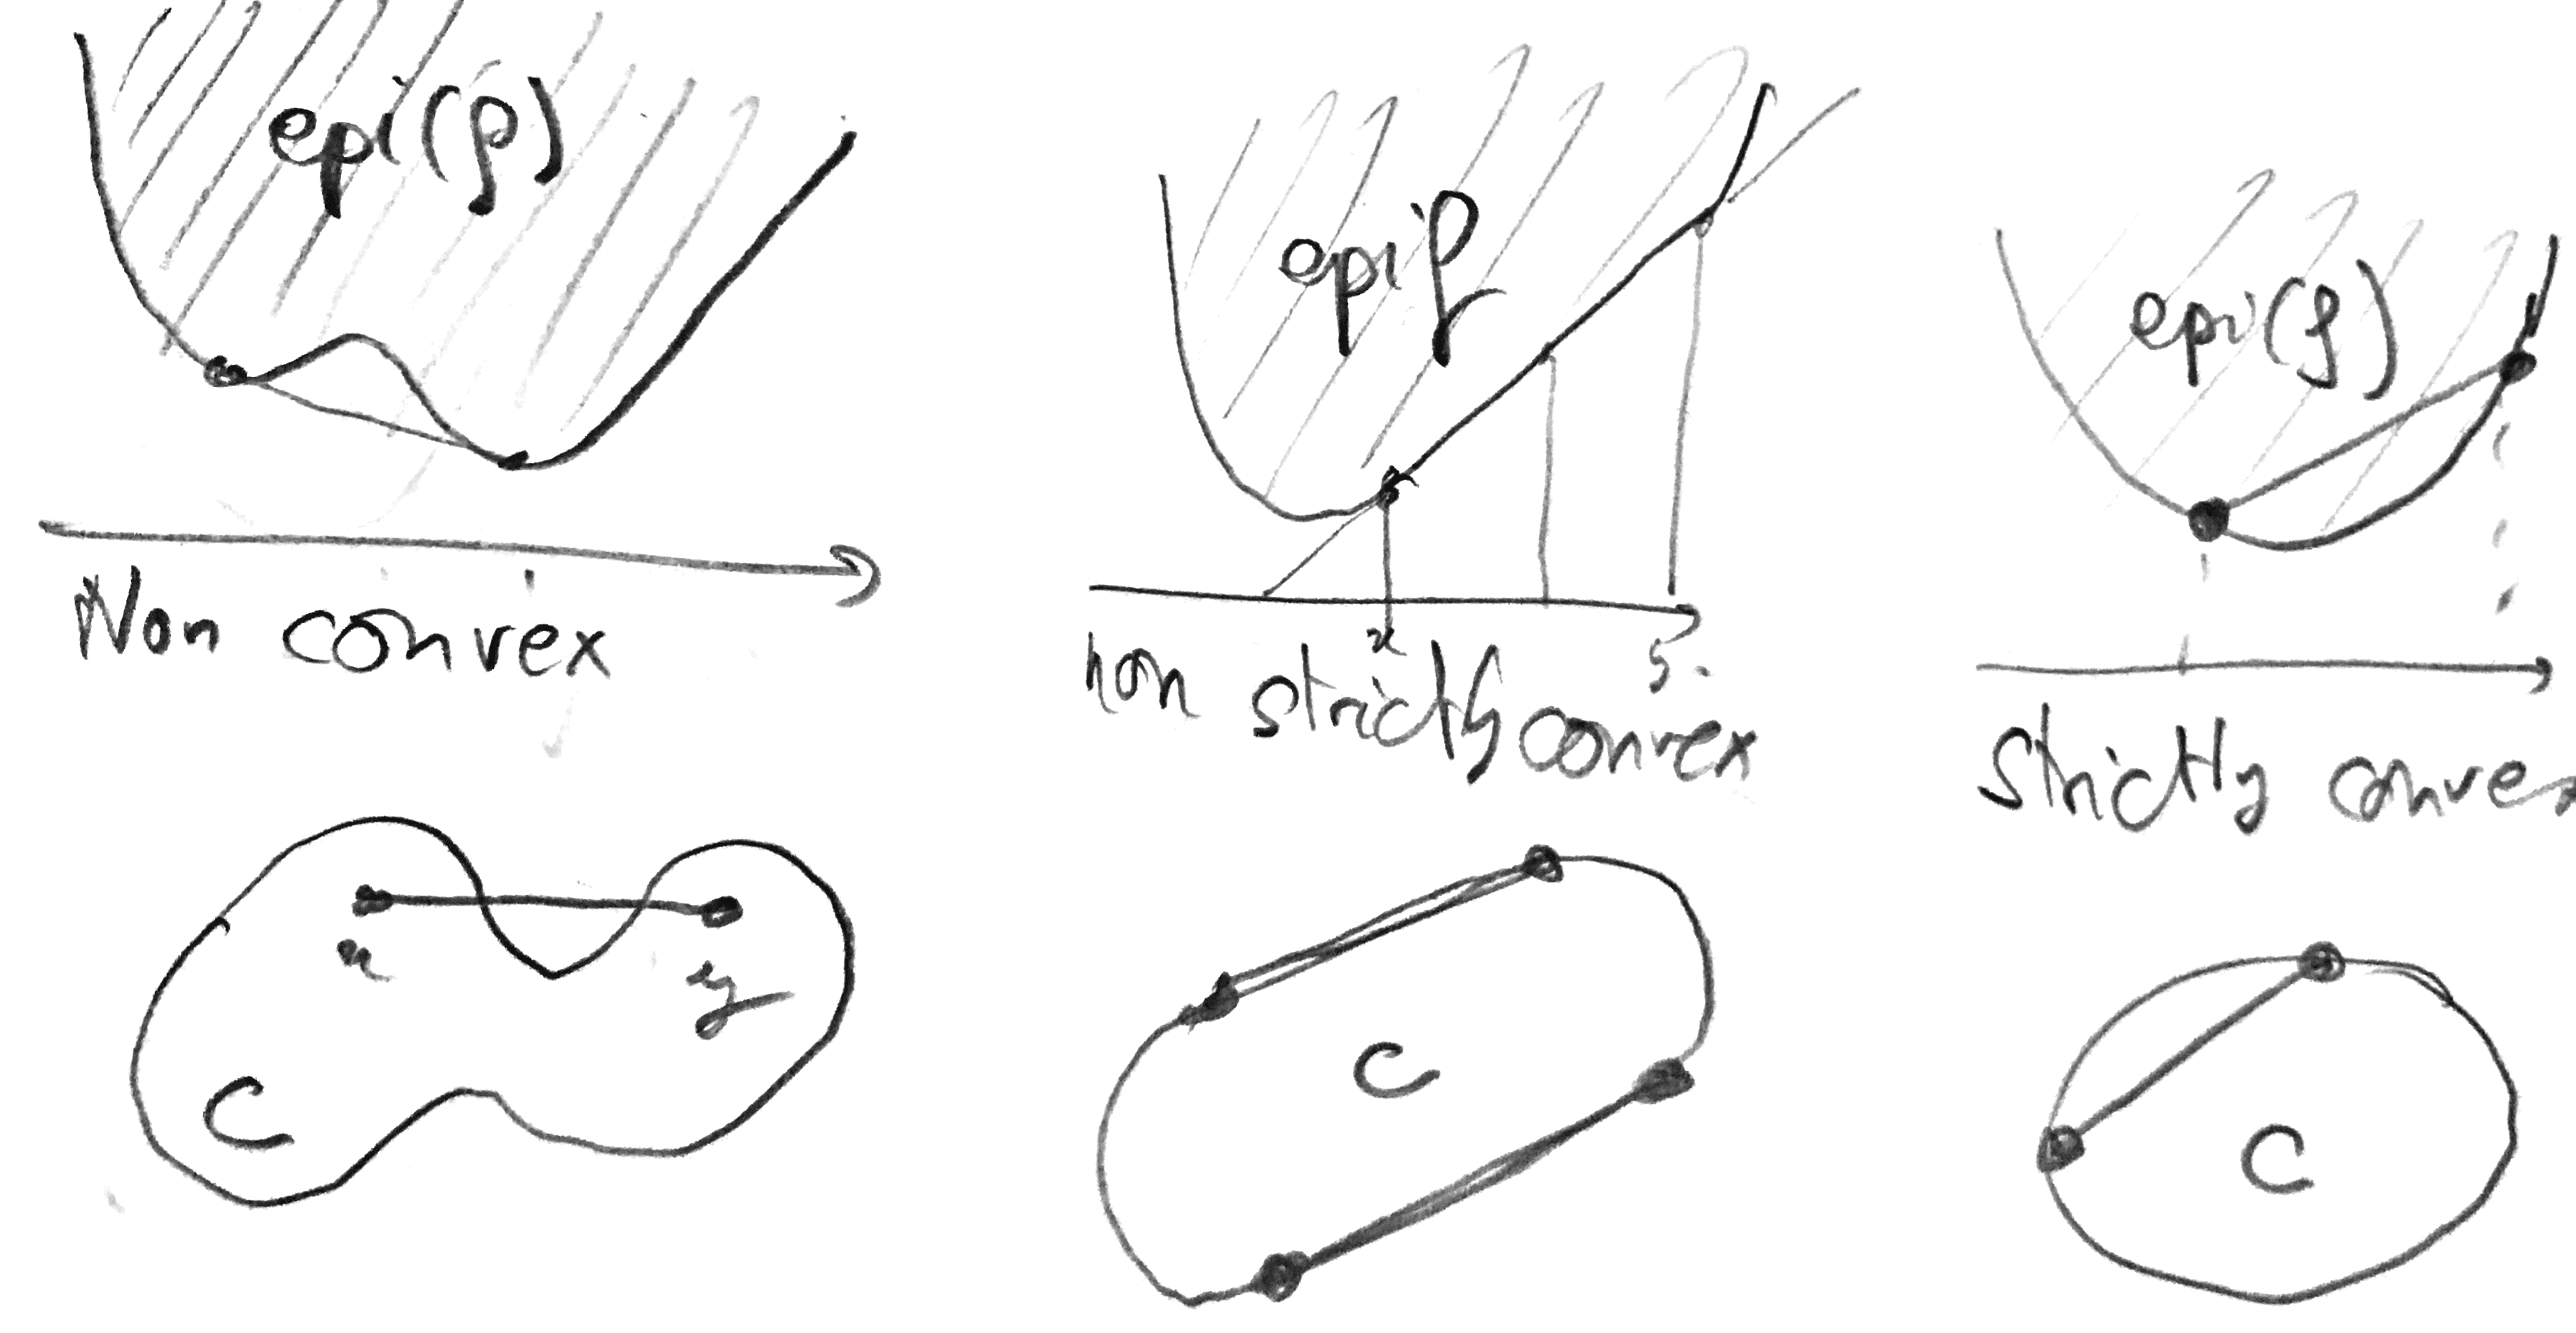
\includegraphics[width=.6\linewidth]{convexity/convex-examples}
%%
\caption{\label{fig-convex-examples}
Convexity and strict convexity for function and sets.}
\end{figure}




In the remaining part of this chapter, we consider convex function $f$ which are proper, i.e. such that $\dom(f) \neq \emptyset$, and that should be lower-semi-continuous (lsc), i.e. such that for all $x \in \Hh$, 
\eq{
	\lim\inf_{y \rightarrow x} f(y)  \geq f(x). 
}
It is equivalent to $\epi(f)$ being a closed convex set.
%
We denote $\Ga_0(\Hh)$ the set of proper convex lsc functions.

%%%%%%%%%%%%%%%%%%%%%%%%%%%%%%%%%%%%%%%%%%%%%%%%%%%%%%%%%%%%%%%%%%%%%%%%%%%%%%%%%%
\subsection{First Order Conditions}

%%%
\paragraph{Existence of minimizers.}

Before looking at first optimality conditions, one has to check that there exists minimizers, which is implied by the l.s.c. property and coercivity.

\begin{prop}
	If $f$ is l.s.c. and coercive (i.e. $f(x)\rightarrow +\infty$ as $x \rightarrow +\infty$), then there exists a minimizer $x^\star$ of $f$. 
\end{prop}

\begin{proof}
Since $f$ is coercive, it is bounded from bellow, one can consider a minimizing sequence $(x_n)_n$ such that $f(x_n) \rightarrow \min f$. 
%
Since $f$ is l.s.c., this implies that the sub-level set of $f$ are closed, and coercivity imply they are bounded, hence compact. One can thus extract from $(x_n)_n$ a converging sub-sequence $(x_{n(p)})_p$, $x_{n(p)} \rightarrow x^\star$. Lower semi-continuity implies that $\min f = \lim_p f(x_{n(p)}) \geq f(x^\star)$, and hence $x^\star$ is a minimizer.
\end{proof}

This existence proof is often called the ``direct method of calculus of variation''.
%
Note that if the function $f$ is in $\Ga_0(\Hh)$, then the set of minimizer $\argmin f$ is a closed convex set, and all local minimizers (i.e. minimizer of the function restricted to an open ball) are global one. If it is furthermore strictly convex, then there is a single minimizer. 

%%%
\paragraph{Sub-differential.}

The sub-differential at $x$ of such a $f$ is defined as
\eq{
	\partial f(x) \eqdef \enscond{u \in \Hh^*}{ \forall y, f(y) \geq f(x) + \dotp{u}{y-x} }.
}
We denote here $\Hh^* = \RR^N$ the set of ``dual'' vector. Although in finite dimensional Euclidean space, this distinction is not needed, it helps to distinguish primal from dual vectors, and recall that the duality pairing implicitly used depends on the choice of an inner product.
%
The sub-differential $\partial f(x)$ is thus the set of ``slopes'' $u$ of tangent affine planes $f(x) + \dotp{u}{z-x}$ that fits bellow the graph of $f$. 


\wrapf{convexity/subdifferential}{The subdifferential}
Note that $f$ being differentiable at $x$ is equivalent to the sub-differential being reduced to a singleton (equal to the gradient vector)
\eq{
	\partial f(x) = \{ \nabla f(x) \}. 
}
Informally, the ``size'' of $\partial f(x)$ controls how smooth $f$ is at $x$.

Note that one can have $\partial f(x) = \emptyset$, for instance if $x \notin \dom(f)$. Note also that one can still have $x \in \dom(f)$ and $\partial f(x) =�\emptyset$, for instance take $f(x)=-\sqrt{1-x^2} + \iota_{[-1,1]}(x)$ at $x=\pm 1$. 

Since $\partial f(x) \subset \Hh^*$ is an intersection of half space, it is a closed convex set.
%  and it is non-empty if and only if $x \in \dom(f)$.
%
The operator $\partial f : \Hh \mapsto 2^{\Hh^*}$ is thus ``set-valued'', and we often denote this as $\partial f : \Hh \hookrightarrow \Hh^*$.

\begin{rem}[Maximally monotone operator]
The operator $\partial f$ is particular instance of so-called monotone operator, since one can check that $U=\partial f$ satisfies 
\eq{
	\foralls (u,v) \in U(x) \times U(y), \quad
		\dotp{y-x}{v-u} \geq 0. 
}
In the 1-D setting, being monotone is the same as being an increasing map.
%
Sub-differential can also be shown to be maximally monotone, in the sense that such an operator is not striclty included in the graph of another monotone operator. 
%
Note that there exists monotone maps which are not subdifferential, for instance $(x,y) \mapsto (-y,x)$. 
% 
Much of the theory of convex analysis and convex optimization can be extended to deal with arbitrary maximally monotone-maps in place of subdifferential, but we will not pursue this here.
\end{rem}

A prototypical example is the absolute value $f(x)=|\cdot|$, and writing conveniently $\partial f(x) = \partial |\cdot|(x)$, one verifies that
\eq{
	\partial |\cdot|(x) = 
	\choice{
		-1 \qifq x < 0, \\
		+1 \qifq x > 0, \\
		{[-1,1]} \qifq x=0.
	}
}

\begin{figure}
\centering
%%
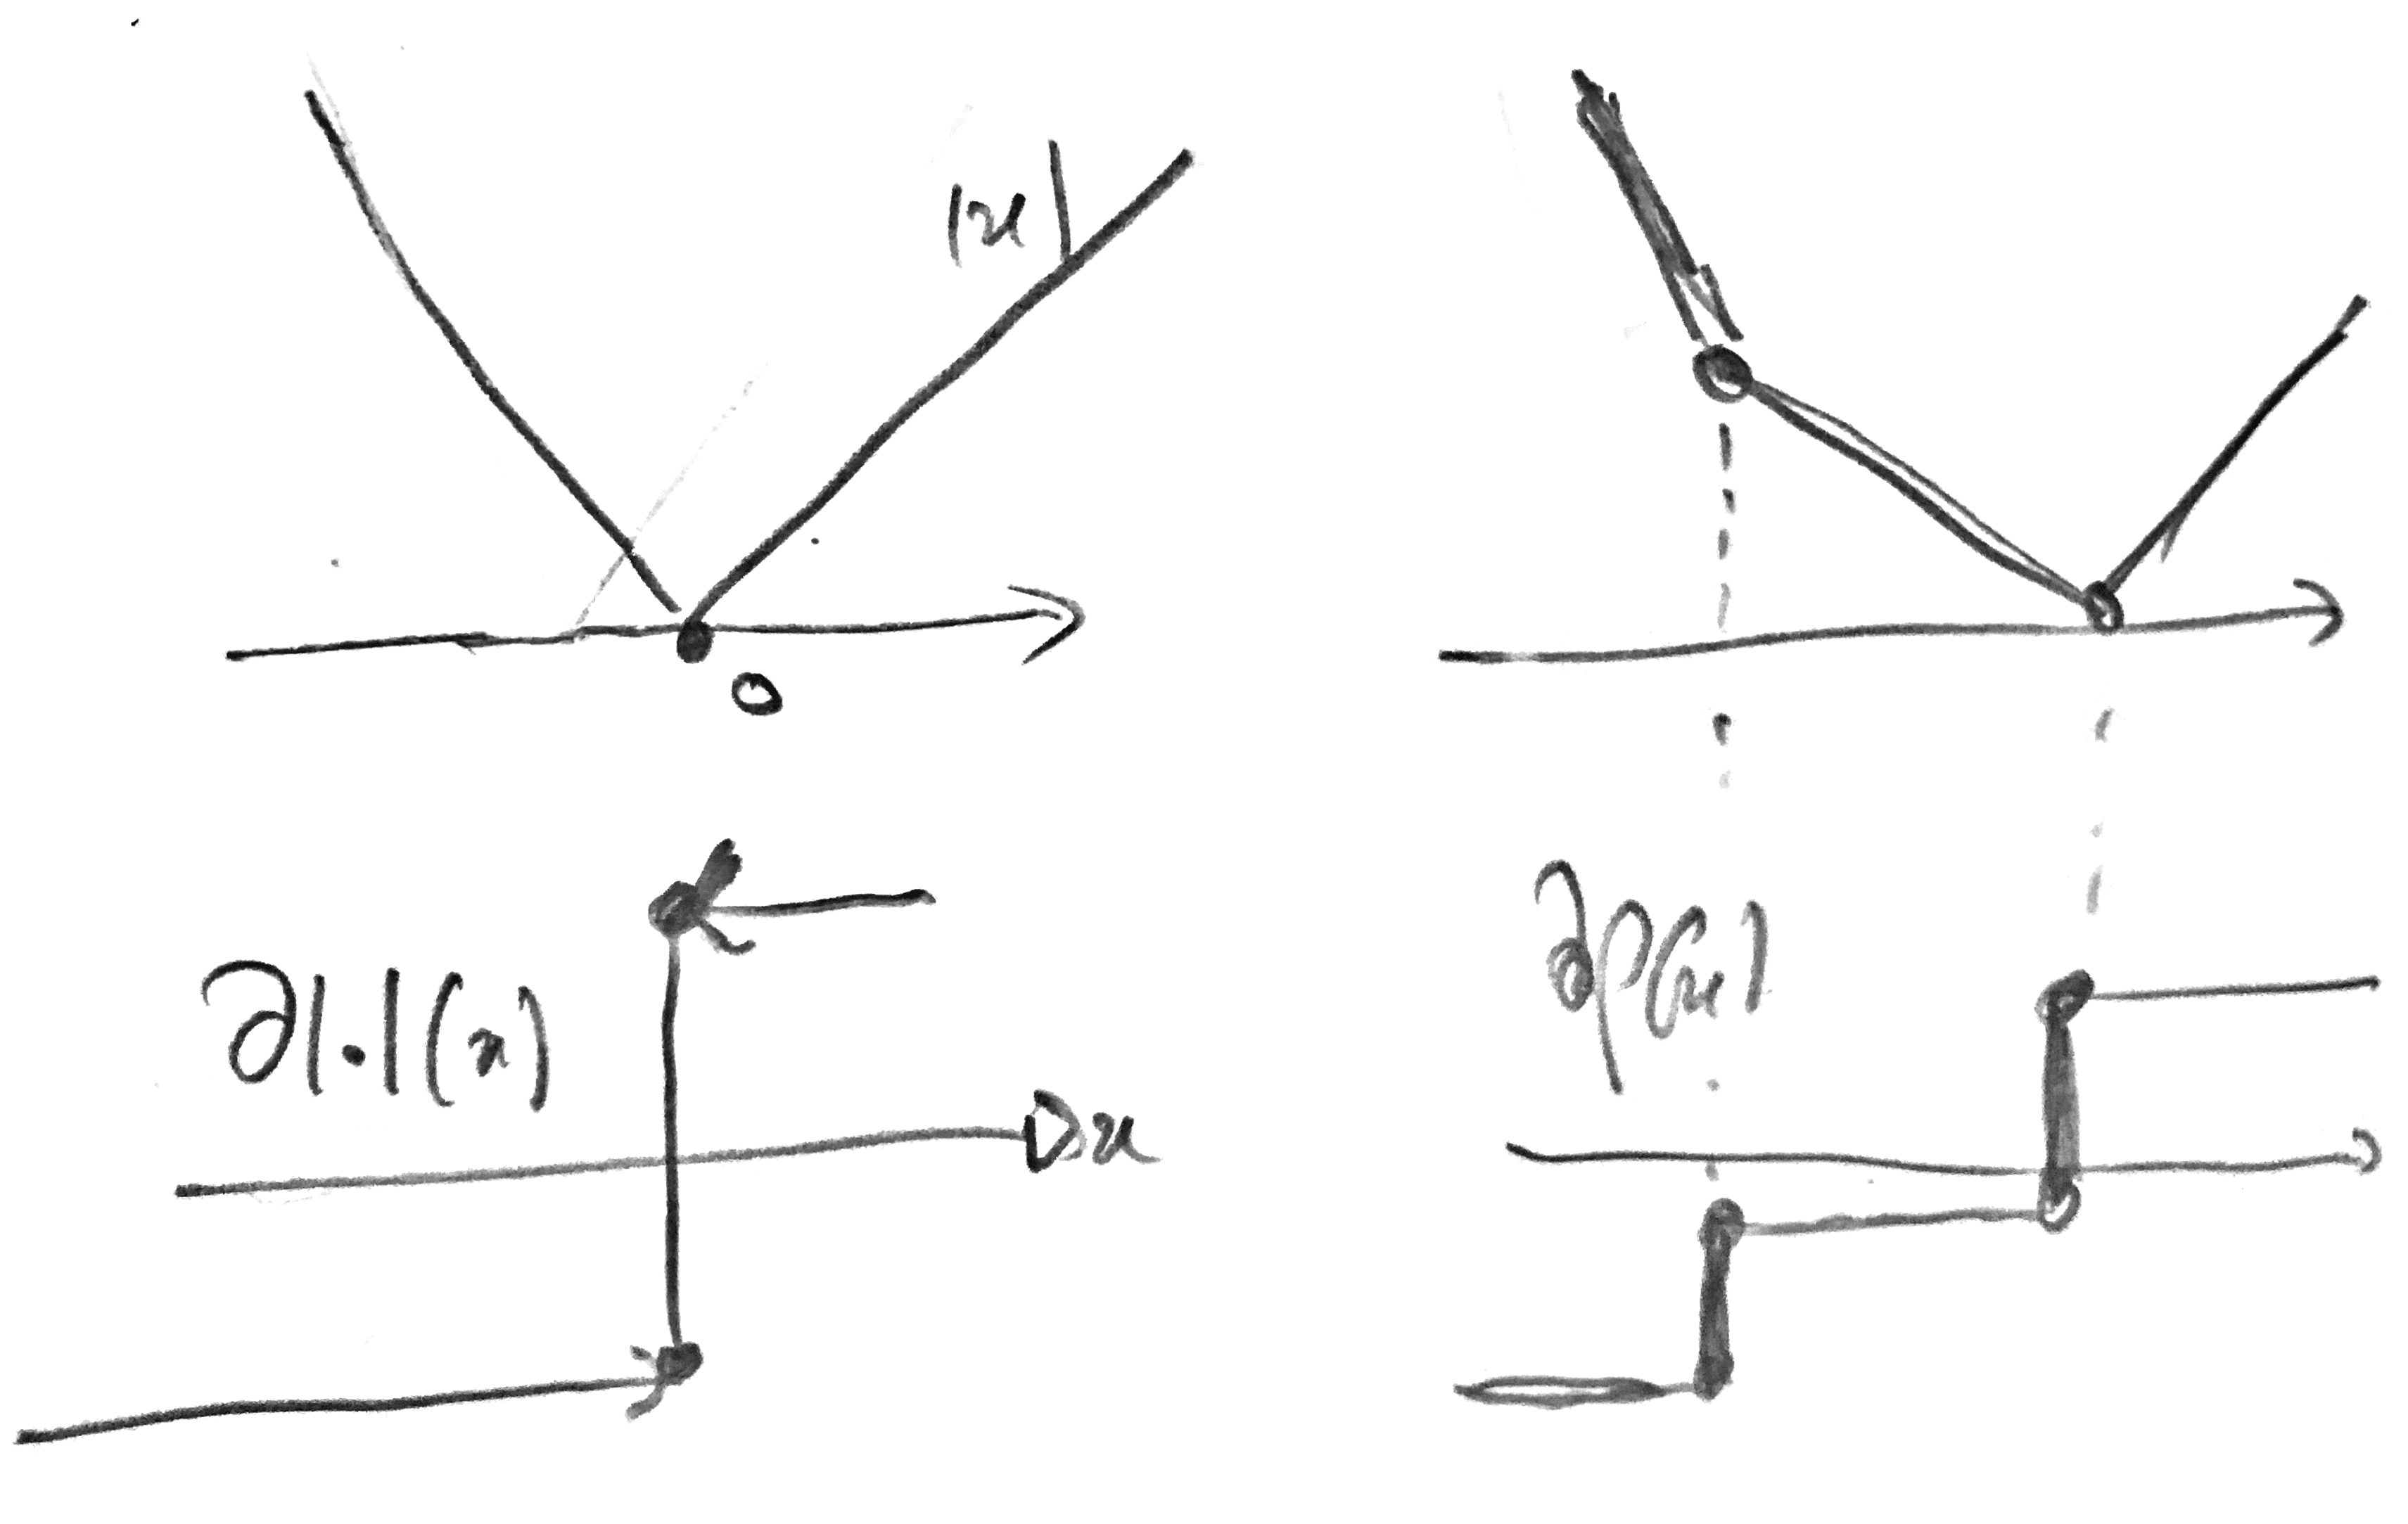
\includegraphics[width=.6\linewidth]{convexity/subdiff-l1}
%%
\caption{\label{fig-subdiff-l1}
Subdifferential of the absolute value and a piecewise affine convex function.}
\end{figure}







%%%
\paragraph{First Order Conditions.}

The subdifferential is crucial for this simple but extremely important proposition.

\begin{prop}
	$x^\star$ is a minimizer of $f$ is and only if $0 \in \partial f(x^\star)$.
\end{prop}
\begin{proof}
	One has
	\eq{
		x^\star \in \argmin f
		\quad\Leftrightarrow\quad
		\pa{ \forall y, f(x^\star) \leq f(y) + \dotp{0}{x^\star-y} }
		\quad\Leftrightarrow\quad
		0 \in \partial f(x^\star).
	}
\end{proof}

%%%
\paragraph{Sub-differential calculus.}

There is a large set of calculus rules that allows to simplify the computation of sub-differentials. For decomposable function $f(x_1,\ldots,x_K)=\sum_{k=1}^K f_k(x_k)$, the sub-differential is the product of the sub-differentials
\eq{
	\partial f(x_1,\ldots,x_K) = \partial f_1(x_1) \times \ldots \times \partial f_K(x_K).
}
This can be used to compute the sub-differential of the $\ell^1$ norm $\norm{x}_1=\sum_{k=1}^N |x_k|$
\eq{
	\partial \norm{\cdot}_1(x) = \prod_{k=1}^N \partial |\cdot|(x_k)
}
which is thus an hyper rectangle. This means that, denoting $I = \supp(x)$, one has $u \in \partial \norm{\cdot}_1(x)$ is equivalent to 
\eq{
	u_I = \sign(x_I)
	\qandq
	\norm{u_{I^c}}_\infty \leq 1.
}

A tricky problem is to compute the sub-differential of the sum of two functions. If one of the two function is continuous at $x$ (i.e. it has a finite value), then 
\eq{
	\partial (f+g)(x) = \partial f(x) \oplus \partial g(x) = \enscond{u+v}{(u,v) \in \partial f(x) \times \partial g(x)}
}
where $\oplus$ thus denotes the Minkowski sum. For instance, if $f$ is differentiable at $x$, then 
\eq{
	\partial (f+g)(x) = \nabla f(x) + \partial g(x) = \enscond{\nabla f(x) + v }{ v \in \partial g(x) }.
}
Positive linear scaling is simple to handle
\eq{
	\foralls \la \in \RR_+, \quad
	\partial (\la f)(x) = \la (\partial f(x)). 
}

The chain rule for sub-differential is difficult since in general composition does not work so-well with convexity. 
%
The only simple case is composition with linear functions, which preserves convexity. Denoting $A \in \RR^{P \times N}$ and $f \in \Ga_0(\RR^P)$, one has that $f \circ A \in \Ga_0(\RR^N)$ and
\eq{
	\partial (f \circ A)(x) = A^* (\partial f)(Ax) \eqdef \enscond{A^* u}{ u \in \partial f(Ax) }. 
}


%%%
\paragraph{Normal cone.}


The sud-differential of an indicator function is a convex cone, the so-called normal cone to the constraint
\eq{
	\foralls x \in \Cc, \quad \partial \iota_\Cc(x) = \Nn_\Cc(x) \eqdef \enscond{ v }{ \foralls z \in \Cc, \dotp{z-x}{v} \leq 0 }.
}
Note that for $x \notin \Cc$, $\partial  \iota_\Cc(x) = \emptyset$.
%
For an affine space $\Cc = a+\Vv$ where $\Vv \subset \Hh$ is a linear space, then $\Nn_\Cc(x)=\Vv^\bot$ is the usual orthogonal for linear spaces. If $x \in \inter(\Cc)$ is in the interior of $\Cc$, then $\Nn_\Cc(x)=\{0\}$. In some sense, the more non-regular the boundary of $\Cc$ is at $x$, the larger is the normal cone. 






\wrapf{convexity/normal-cone}{Normal cones}
The normal cone is a way to express first order condition for constrained problem
\eq{
	\umin{x \in \Cc} f(x)
}
which reads, if $f$ is continuous
\eq{
	0 \in \partial f(x) + \partial \iota_{\Cc}(x)
	\quad\Leftrightarrow\quad
	\exists \xi \in \partial f(x), - \xi \in \Nn_\Cc(x)
	\quad\Leftrightarrow\quad
	\partial f(x) \cap (-\Nn_\Cc(x)) \neq \emptyset.
}
If $f$ is differentiable, it reads $-\nabla f(x) \in \Nn_\Cc(x)$.



%%%%%%%%%%%%%%%%%%%%%%%%%%%%%%%%%%%%%%%%%%%%%%%%%%%%%%%%%%%%%%%%%%%%%%%%%%%%%%%%%%
%%%%%%%%%%%%%%%%%%%%%%%%%%%%%%%%%%%%%%%%%%%%%%%%%%%%%%%%%%%%%%%%%%%%%%%%%%%%%%%%%%
%%%%%%%%%%%%%%%%%%%%%%%%%%%%%%%%%%%%%%%%%%%%%%%%%%%%%%%%%%%%%%%%%%%%%%%%%%%%%%%%%%
\section{Convex Duality}
\label{sec-cvx-duality}

Duality is associated to a particular formulation of the optimization problem, so that for instance making change of variables results in a different duality. 

%%%%%%%%%%%%%%%%%%%%%%%%%%%%%%%%%%%%%%%%%%%%%%%%
\subsection{Lagrange Duality}

We consider a minimization of the form
\eql{\label{eq-lagrange-primal}
	p^\star = \umin{x \in \RR^N} \enscond{ f(x) }{ Ax=y \qandq g(x) \leq 0 }
}
for a continuous�convex functions $f : \Hh \rightarrow 0$, a matrix $A \in \RR^{P \times N}$ and a function $g : \Hh \rightarrow \RR^Q$ such that each of its coordinates $g_i : \Hh \rightarrow \RR$ are continuous and convex.  
%
Note that it is always the case that equality in convex program corresponds to affine ones. 
%
One can always write a convex minimization problem with positivity constraints in the form~\eqref{eq-lagrange-primal}, although there exists infinite way of doing so (each one giving a different duality formula). 

Here we have assumed for simplicity that $f$ is continuous, i.e. $\dom(f)=\RR^N$.
%
The following exposition can be generalized to $\dom(f)$ being arbitrary, but this is more technical. For the sake of simplicity, we thus assume all the constraint defining the domain are encoded in $Ax=y$ and $g(x) \leq 0$


Note that it is possible to generalized the previous Lagrange duality results by replacing ``$x \geq 0$'' by ``$X \succeq 0$'' where $X$ is a matrix (and in fact even more generally using convex cones). 

We use the following fact
\eq{
	\usup{u \in \RR^P}�\dotp{r}{u} = \choice{
		0 \qifq r=0, \\
		+\infty \qifq r \neq 0, 
	}
	\qandq
	\usup{v \in \RR_+^Q}�\dotp{s}{v} = \choice{
		0 \qifq s \leq 0, \\
		+\infty \text{ otherwise}, 
	}
}
to encode the constraints $r=Ax-y=0$ and $s=g(x) \leq 0$.

One can represent the constraints appearing in~\eqref{eq-lagrange-primal} conveniently using a maximization over so-called Lagrange multipliers
\eq{
	p^\star = \uinf{x} \umax{u \in \RR^P, v \in \RR_+^Q } \Ll(x,u,v) \eqdef f(x) + \dotp{Ax-y}{u} + \dotp{g(x)}{v} .
}

It is tempting to inverse the inf and the sup, and study 
\begin{align}\label{eq-lagrange-dual}
	d^\star = \usup{(u,v) \in \RR^P \times \RR_+^Q } F(u,v) &\eqdef \uinf{x}  f(x) + \dotp{Ax-y}{u} + \dotp{g(x)}{v}.
\end{align}
One remarks that $F$ is a concave function (as being the minimum of linear forms), and this ``dual'' problem is thus a maximization of a concave function. 


The following proposition is the so-called weak duality, which assert that values of the dual problems always lower bounds values of the primal one

\begin{prop}
	One always has, for all $(u,v) \in \RR^P \times \RR_+^Q$, % for $x$ such that $Ax=y, g(x) \leq 0$ and 
	\eq{
		F(u,v) \leq p^\star \qarrq d^\star \leq p^\star.
	}
\end{prop}
\begin{proof}
	Since $g(x) \leq 0 $ and $v \geq 0$, one has $\dotp{g(x)}{v} \leq 0$, and since $Ax=y$, one has $\dotp{Ax-y}{u}=0$, so that 
	\eq{
		\Ll(x,u,v) \leq f(x) \qarrq F(u,v) = \uinf{x} \Ll(x,u,v) \leq \uinf{x} f(x) = p^\star.
	}
\end{proof}

The following fundamental theorem, more difficult to prove, gives a sufficient condition (so-called qualification of the constraints) such that one actually has equality.

\begin{thm}\label{thm-strong-duality}
	If 
	\eql{\label{eq-slater} 
		\exists x_0 \in \RR^N, \quad
			Ax_0=y \qandq g(x_0)<0, 
	}
	then $p^\star=d^\star$. Furthermore, $x^\star$ and $(u^\star,v^\star)$ are  solutions of respectively~\eqref{eq-lagrange-primal} and~\eqref{eq-lagrange-dual} if and only if
	\begin{align}
		\label{eq-lagr-dual-1}  & Ax^\star=y, \quad g(x^\star) \leq 0, \quad u^\star \geq 0 \\
		\label{eq-lagr-dual-2} 0 &\in \partial f(x^\star) + A^*u^\star + \sum_i v_i^\star \partial g_i(x^\star) \\
		\label{eq-lagr-dual-3}  \foralls i, \quad & u_i^\star g_i(x^\star) = 0
	\end{align}
\end{thm}

The existence of such an $x_0$ is called ``constraint qualification'', and as written here, this corresponds to the so-called ``Slater'' qualification condition (many other weaker sufficient conditions exist). 

Condition~\eqref{eq-lagr-dual-1} is simply the primal and dual constraints. 
%
Condition~\eqref{eq-lagr-dual-2} is the first order condition for the minimization of $\Ll(x,u,v)$ over $x$.
%
Condition~\eqref{eq-lagr-dual-3} is the first order condition for the maximization of $\Ll(x,u,v)$ over $(u,v)$.
%
These three conditions are often referred to as ``Karush-Kuhn-Tucker'' (KKT) conditions, and under a constraint qualification condition, they are necessary and sufficient condition for optimality. 


The last condition $u_i^\star g_i(x^\star) = 0$ (so called ``complementary slackness'') states that if $g_i(x^\star)<0$ (the constraints is not saturated) then $u_i=0$, and also that if $u_i>0$ then $g_i(x^\star)=0$.

Note that it is possible to weaken the hypotheses of this theorem, for the linear constraints of the form $g_i(x) = \dotp{x}{h_i} - c_i \leq 0$, by replacing the $g_i(x_0)<0$ by the weaker condition $\dotp{x_0}{h_i} \leq c_i$.

One can generalize this theorem to the setting where $\dom(f)$ is not equal to $\RR^N$ (i.e. it is not continuous, and thus integrates extra constraint beside the $\leq$). In this case, one has to add the extra constraint $x_0 \in \relint(\dom(f))$.
	
Theorem~\ref{thm-strong-duality} generalizes the necessary conditions provided by Lagrange multipliers for equality constrained optimization. The setting is both more complex because one can deal with inequalities that might be saturated (so this introduce positivity constraints on the multipliers $v$) but also simpler because of convexity (which thus gives also necessary conditions).

As a simple example, we now derive the dual for a simple linear projection problem. A more complicated computation is carried over in Section~\ref{sec-duality-lasso}�for the Lasso. We consider
\begin{align*}
	p^\star = \umin{Ax=y} \frac{1}{2}\norm{x-z}^2 &= \umin{x} \umax{u} \frac{1}{2}\norm{x-z}^2 + \dotp{Ax-y}{u}
	= \umax{u} F(u) = \umin{x} \frac{1}{2}\norm{x-z}^2 + \dotp{Ax-y}{u}, 
\end{align*}
where we used the fact that strong duality holds because only linear constraints are involved.
%
For each $u$, the optimal $x$ satisfies $x-z+A^*u$, i.e. $x=z-A^*u$, so that 
\eq{
	F(u) = \frac{1}{2}\norm{A^*u}^2 + \dotp{A(z-A^*u)-y}{u} = -\frac{1}{2}\norm{A^*u}^2 + \dotp{u}{Az-y}.
}
Weak duality states $p^\star \geq F(u)$ for any $u$, and $p^\star = F(u^\star)$ where the optimal $u^\star$ satisfies $AA^*u = Az-y$. If $y \in \Im(A)$, then such a $u^\star$ exists and can be chosen as $u^\star = u=(AA^*)^{-1} (Az -y)$, and the (unique) primal solution reads 
\eql{\label{eq-proj-aff}
	x^\star = \Proj_{A\cdot=y}(z) (\Id-A^+A)z - A^+y.
}

%%%%%%%%%%%%%%%%%%%%%%%%%%%%%%%%%%%%%%%%%%%%%%%%
\subsection{Legendre-Fenchel Transform}

In order to simplify and accelerate computation involving Lagrange duality, it is very convenient to introduce a particular transformation of convex functions the Legendre-Fenchel transform. In some sense, it is the canonical ``isomorphisms'' (pairing) between convex functions. In spirit, is plays a similar role for convex function as the Fourier transform for signal or images. 

For $f \in \Ga_0(\Hh)$, we define its Legendre-Fenchel transform as
\eql{\label{eq-fenchel-transf}
	f^*(u) \eqdef�\usup{x} \dotp{x}{u} - f(x).
}
Being the maximum of affine functional, one obtains that $f^*$ is itself a convex function, and that in fact $f^\star \in \Ga_0(\Hh^*)$. One can prove the following fundamental bi-duality result.

\begin{thm}
One has
\eq{
	\foralls f \in \Ga_0(\Hh), \quad (f^{*})^* = f. 
}
\end{thm}

In fact, $f^*$ is convex even in the case where $f$ is not, and $f^{**}$ is the convex envelop of $f$ (i.e. the largest convex function smaller than $f$). \todo{drawing}


One has the following basic property relating the sub-differentials of $f$ and $f^*$.

\begin{prop}
One has $\partial f^* = (\partial f)^{-1}$, where the inverse of a set valued map is defined in~\eqref{eq-inv-setvalued}, and 
\eq{
	\foralls (x,y), \quad \dotp{x}{y} \leq f(x) + f^*(y)
	\qandq
	\dotp{x}{y} = f(x) + f^*(y) 
	\quad\Leftrightarrow\quad x \in \partial f^*(y)
	\quad\Leftrightarrow\quad y \in \partial f(x).
}
\end{prop}

\begin{prop}\label{prop-dual-lp}
	For $1/p+1/q=1$, 
	\eq{
		( \iota_{\norm{\cdot}_p \leq 1} )^* = \norm{\cdot}_q
		\qandq
		( \norm{\cdot}_q  )^* =  \iota_{\norm{\cdot}_p \leq 1}
	}
\end{prop}


Let us now give some example of Legendre transform. 

\begin{prop}\label{eq-example-legendre}
	For $f(x)=\frac{1}{2}\dotp{Ax}{x} - \dotp{b}{x}$ with $A$ inversible, then $f^*(u) = \frac{1}{2}\dotp{A^{-1} u}{u} - \frac{1}{2}\dotp{A^{-1} b}{b}$.
	In particular, for $f=\norm{\cdot}^2/2$, then $f^*=f$. 
	One has\todo{check}
	\eq{
		f(\cdot-z)^* = f + \dotp{z}{\cdot}, \quad
		(f + \dotp{z}{\cdot})^* = f(\cdot-z), \quad
		(\la f)^* = \la f^*(\cdot/\la).		
	}
\end{prop}
\begin{proof}
	One has $f^*(u) = \dotp{Ax^\star}{x^\star} - \dotp{b}{x^\star}$ where $x^\star$ solves
	\eq{
		u = Ax^\star-b \qarrq
		x^\star = A^{-1} u + A^{-1} b.
	}
	Hence
	\eq{
		f^*(u)  = \frac{1}{2}\dotp{A A^{-1} ( u +  b )}{A^{-1}( u +  b)} - \dotp{b}{A^{-1} (u + b)}
			= \frac{1}{2}\dotp{A^{-1} u}{u} 
			- \frac{1}{2}\dotp{A^{-1} b}{b}
	}
	
\end{proof}

%%%%
\paragraph{Legendre transform and smoothness.}

While the Fourier transform is a pairing between smoothness and decay (see Section~\ref{}), the Legendre-Fenchel is really a pairing between smoothness and strong convexity. This can be intuitively seen by the fact that the Legendre-Fenchel inverts the sub-differentials~\eqref{} and hence when the functions involved are $\Cc^2$, it inverse the Hessians 
\eq{
	\partial^2 f(x) = ( \partial^2 f^*(y) )^{-1} \quad \text{at} \quad y = \nabla f(x).
}
This relation between Hessian can be seen as implying the exchange of strong convexity and uniform bound on the Hessian, as detailed in Proposition~\ref{prop-smooth-strong}.

\begin{prop}
	One has
	\eq{
		\nabla f \text{ is $L$-Lipschitz } 
		\quad\Longleftrightarrow\quad
		\nabla f^* \text{ is $\mu$-strongly convex.} 
	}
\end{prop}

This results suggests a way to smooth any function $f$. Instead of doing a convolution, one can use the infimal convolution
\eq{
	(f \otimes g)(x) \eqdef \usup{ y+y'=x } f(y) + g(y').
}
One can check that if $(f,g)$ are convex, so is $f \otimes g$, and that the Legendre transform actually exchanges sum and inf-convolution
\eq{
	( f+g )^* = f \otimes g 
	\qandq 
	( f \otimes g )^* = f + g.
}
The Moreau-Yosida regularization of $f$ is corresponds to a $\mu$-strict-convexification of $f^*$, i.e.
\eql{\label{eq-moreau-yosida}
	f_\mu \eqdef f \otimes (\frac{1}{2\mu}\norm{\cdot}^2) = ( f^* + \frac{\mu}{2}\norm{\cdot}^2 )^*.
}
Since $f^* + \frac{\mu}{2}\norm{\cdot}^2$ is at least $\mu$-strongly convex, then $f_\mu$ as a $1/\mu$-Lipchitz gradient.

As an example, the Moreau-Yosida regularization of the absolute value reads
\eq{
	(|\cdot|_\mu)(x) = 
	\choice{
		\frac{1}{2\mu}x^2 \qifq |x| \leq \mu, \\
		|x|-\frac{\mu}{2} \qifq |x|>\mu.
	}
}
This should be compared with the regularization $\sqrt{x^2+\mu^2}$ (which is above the curve) that we used previously. \todo{add drawing}



%%%%%%%%%%%%%%%%%%%%%%%%%%%%%%%%%%%%%%%%%%%%%%%%
\subsection{Fenchel-Rockafellar Duality}

%It is possible to express the Lagrange duality in term of Fenchel transform. Indeed for instance, re-write~\eqref{eq-lagrange-primal} as
%\eq{
%	\umin{(x,z) \in \RR^N} \enscond{ f(x) }{ Ax=y, x=z \qandq g(z) \leq 0 }
%}
%and then form the Lagrange dual
%\begin{align*}
%	 \umax{u \in \RR^P, v \RR_-^Q, w \in \RR^N } &\umin{x,z}  f(x) + \dotp{Ax-y}{u} + \dotp{x-z}{w} + \dotp{g(z)}{v} \\
%	 \umax{u \in \RR^P, v \RR_-^Q, w \in \RR^N } &\umin{x}�f(x) + \dotp{x}{A^*u+w} + \sum_i \umin{z} - \dotp{z}{w} + g_i(z) {v_i} \\
%\end{align*}

Very often the Lagrange dual can be expressed using the conjugate of the function $f$. We give here a particularly important example, which is often called Fenchel-Rockafellar Duality. 

We consider the following structured minimization problem
\eql{\label{eq-fench-rock-basicpb}
	p^\star = \uinf{x} f(x) + g(Ax).	
}
Re-writing it as 
\eq{
	\uinf{y=Ax} f(x) + g(y), 
}
we can form the primal-dual problem
\eq{
	\uinf{(x,y)} \usup{u} f(x) + g(y) + \dotp{Ax-y}{u}. 
}
If sufficient condition on the domain of $(f,g)$ holds (such as those stated in Theorem~\ref{}), one one can exchange the min and the max and obtains the dual problem
\begin{align}\label{eq-deriv-rock-fench}
	d^\star &= \usup{u} \umin{(x,y)} f(x) + g(y) + \dotp{Ax-y}{u} \\
	&= \usup{u} \pa{ \umin{x} \dotp{x}{A^* u} + f(x) } + \pa{ \umin{y} -\dotp{y}{u} + g(y) } 
\end{align}
which leads to the celebrated Fenchel-Rockafellar, which we summarize together with qualification sufficient condition ensuring strong duality.

\begin{thm}[Fenchel-Rockafellar]\label{thm-fenchel-Rockafellar}
If 
\eql{\label{eq-qualif-fenchrock}
	0 \in \relint( \dom(g) ) - A \relint( \dom(f) )
}
the one has the following strong duality
\begin{align}\label{eq-fenchel-Rockafellar}
	\uinf{x} f(x) + g(Ax) &= \uinf{x} \usup{u} \Ll(x,u) 
	= \usup{u} \uinf{x}\Ll(x,u)  
	= \usup{u} - f^*(-A^*u) - g^*(u)
\end{align}
\eq{
	\qwhereq  \Ll(x,u)  \eqdef f(x) + \dotp{Ax}{u}  - g^*(u).
}
Furthermore one has that $(x^\star,u^\star)$ is a pair of optimal primal-dual solutions if and only if
\eql{\label{eq-primal-dual}
	-A^* u^\star \in \partial f(x^\star)  
	\qandq
	A x^\star \in  \partial g^*(u^\star).
}
\end{thm}

Condition~\eqref{eq-qualif-fenchrock} is the constraint qualification ensuring that one can inverse the inf and the sup in~\eqref{eq-fenchel-Rockafellar}. It can be recovered from Slater's qualification condition~\eqref{eq-slater} when deriving the dual problem as in~\eqref{eq-deriv-rock-fench}.
%
The primal-dual relations~\eqref{eq-primal-dual} are the first order condition along the $x$ and the $u$ variables in minimization and maximization of $\Ll$. They are sometimes summarised in ``matrix'' form 
\eq{
	0 \in 
	\begin{pmatrix}
		\partial f & A^* \\
		-A & \partial g^*
	\end{pmatrix}
	\begin{pmatrix}
		x^\star \\
		u^\star
	\end{pmatrix}.
}
% !TEX root = ../FundationsDataScience.tex

\chapter{Convex Optimization}
\label{chap-conv-duality}

The main references for this chapter are~\cite{chambolle2010introduction,chambolle2016introduction,boyd2004convex}, see also~\cite{parikh2014proximal,boyd2011distributed,beck2014introduction}. 


We consider a general convex optimization problem
\eql{\label{eq-general-pbm} % eq-min-smooth-uncons
	\umin{x \in \Hh} f(x)
}
where $\Hh=\RR^N$ is a finite dimensional Hilbertian (i.e. Euclidean) space, 
and try to devise ``cheap'' algorithms with a low computational cost per iterations. The class of algorithms considered are first order, i.e. they make use of gradient information. 


%%%%%%%%%%%%%%%%%%%%%%%%%%%%%%%%%%%%%%%%%%%%%%%%%%%%%%%%%%%%%%%%%%%%%%%%%%%%%%%%%%
%%%%%%%%%%%%%%%%%%%%%%%%%%%%%%%%%%%%%%%%%%%%%%%%%%%%%%%%%%%%%%%%%%%%%%%%%%%%%%%%%%
%%%%%%%%%%%%%%%%%%%%%%%%%%%%%%%%%%%%%%%%%%%%%%%%%%%%%%%%%%%%%%%%%%%%%%%%%%%%%%%%%%
\section{Gradient Descent Methods}
\label{sec-grad-descent}

We have already encountered the gradient descent method informally in Section~\ref{}�for the regularization of inverse problem. We now give a detailed analysis of the method.

%%%%%%%%%%%%%%%%%%%%%%%%%%%%%%%%%%%%%%%%%%%%%%%%%%%%%%%%%%%%%%%%%%%%%%%%%%%%%%%%%%
\subsection{Gradient Descent}

The optimization program~\eqref{eq-ip-tv-eps} is a example of unconstrained convex optimization of the form~\eqref{eq-general-pbm} where $f : \Hh \rightarrow \RR$ is a $\Cc^1$ function with Lipschitz gradient (so-called ``smooth'' function). Recall that the gradient $\nabla f : \Hh \mapsto \Hh$ of this functional (not to be confound with the discretized gradient $\nabla x \in \Hh$ of $f$) is defined by the following first order relation
\eq{
	f(x+r) = f(x) + \dotp{f}{r}_{\Hh} + O(\norm{r}_{\Hh}^2)
}
where we used $O(\norm{r}_{\Hh}^2)$ in place of $o(\norm{r}_{\Hh})$ (for differentiable function) because we assume here $f$ is of class $\Cc^1$ (i.e. the gradient is continuous). Section~\ref{eq-example-grad} shows typical examples of gradient computation.

For such a function, the gradient descent algorithm is defined as
\eql{\label{eq-grad-desc}
	\iit{x} \eqdef \it{x} - \tau_\ell \nabla f( \it{x} ), 
}
where the step size $\tau_\ell>0$ should be small enough to guarantee convergence, but large enough for this algorithm to be fast.

One also needs to quantify the smoothness of $f$. This is enforced by requiring that the gradient is $L$-Lipschitz, i.e.
\eql{\label{eq-lipsch-grad}\tag{$\Rr_L$}
	\foralls (x,x') \in \Hh^2, \quad
	\norm{ \nabla f(x)-\nabla f(x') } \leq L \norm{x-x'}. 
}
In order to obtain fast convergence of the iterates themselve, it is needed that the function has enough ``curvature'' (i.e. is not too flat), which corresponds to imposing that $f$ is $\mu$-strongly convex
\eql{\label{eq-strong-conv}\tag{$\Ss_\mu$}
	\foralls (x,x'), \in \Hh^2, \quad
	\dotp{\nabla f(x)-\nabla f(x')}{ x-x' } \geq \mu \norm{x-x'}^2. 
}
The following proposition express these conditions as constraints on the hessian for $\Cc^2$ functions.

\begin{prop}
Conditions~\eqref{eq-lipsch-grad} and~\eqref{eq-strong-conv} imply
\eql{\label{eq-above-below-quad}
	\foralls (x,x'), \quad
	f(x') + \dotp{\nabla f(x)}{x'-x} + \frac{\mu}{2}\norm{x-x'}^2
	\leq
	f(x) 
	\leq 
	f(x') + \dotp{\nabla f(x')}{x'-x} + \frac{L}{2}\norm{x-x'}^2.
}
If $f$ is of class $\Cc^2$, conditions~\eqref{eq-lipsch-grad} and~\eqref{eq-strong-conv} are equivalent to
\eql{\label{eq-upper-lower-bound-hess}
	\foralls x, \quad \mu \Id_{N \times N}  \preceq \partial^2 f(x) \preceq L \Id_{N \times N}
}
where $\partial^2 f(x) \in \RR^{N \times N}$ is the Hessian of $f$, and 
where $\preceq$ is the natural order on symmetric matrices, i.e.
\eq{
	A \preceq B \quad\Longleftrightarrow\quad
	\foralls x \in \Hh, \quad \dotp{A u}{u} \leq \dotp{B u}{u}.
}
\end{prop}
\begin{proof}
	We prove~\eqref{eq-above-below-quad}, using Taylor expansion with integral remain
	\eq{
		f(x') - f(x) = \int_0^1 \dotp{\nabla f(x_t)}{x'-x} \d t
		= \dotp{\nabla f(x)}{x'-x} + \int_0^1 \dotp{\nabla f(x_t)-\nabla f(x)}{x'-x} \d t		
	}
	where $x_t \eqdef f+t(x'-x)$.
	%
	Using Cauchy-Schwartz, and then the smoothness hypothesis~\eqref{eq-lipsch-grad}
	\eq{
		f(x') - f(x) \leq \dotp{\nabla f(x)}{x'-x} +  \int_0^1 L \norm{x_t-f} \norm{x'-x} \d t
		\leq \dotp{\nabla f(x)}{x'-x} +  L \norm{x'-x}^2 \int_0^1  t  \d t
	} 
	which is the desired upper-bound. Using directly~\eqref{eq-strong-conv} gives 
	\eq{
		f(x') - f(x) 
		= \dotp{\nabla f(x)}{x'-x} + \int_0^1 \dotp{\nabla f(x_t)-\nabla f(x)}{\frac{x_t-x}{t}} \d t	
		\geq \dotp{\nabla f(x)}{x'-x} + \mu \int_0^1 \frac{1}{t}\norm{x_t-x}^2  \d t
	}
	which gives the desired result since $\norm{x_t-x}^2 / t = t \norm{x'-x}^2$.
\end{proof}

The relation~\eqref{eq-above-below-quad} shows that a smooth (resp. strongly convex) functional is bellow a quadratic tangential majorant (resp. minorant). 

Condition~\eqref{eq-upper-lower-bound-hess} thus reads that the singular values of $\partial^2 f(x)$ should be contained in the interval $[\mu,L]$. The upper bound is also equivalent to $\norm{\partial^2 f(x)}_{\text{op}} \leq L$ where $\norm{\cdot}_{\text{op}}$ is the operator norm, i.e. the largest singular value. 
%
In the special case of a quadratic function $\Qq$ of the form~\eqref{eq-quad-func}, $\partial^2 f(x)=A$ is constant, so that $[\mu,L]$ can be chosen to be the range of the singular values of $A$.

The following theorem ensure the convergence of the gradient descent with a linear speed.

\begin{thm}\label{thm-gradsec-strong-conv}
	If $f$ satisfy conditions~\eqref{eq-lipsch-grad} and~\eqref{eq-strong-conv}, assuming there exists $(\tau_{\min},\tau_{\max})$ such that
	\eql{\label{eq-descent-step-cond}
		0 < \tau_{\min} \leq \tau_\ell \leq \tau_{\max} < \frac{2 \mu}{L}
	}
	then there exists $0 \leq \rho<1$ such that 
	\eql{\label{eq-global-linrate-grad}
		\norm{ \it{x}-x^\star } \leq \rho^\ell \norm{\itz{x}-x^\star}
	} 
	where $x^\star$ is the unique solution to~\eqref{eq-min-smooth-uncons}. 
\end{thm}
\begin{proof}
	Since $\nabla f(x^\star)=0$, one has
	\eq{
		\iit{x}-x^\star = (\it{x}-x^\star) - \tau_\ell ( \nabla f(\it{x})-\nabla f(x^\star) ).
	}
	Hence, using strong convexity and Lipschitz gradient
	\begin{align*}
		\norm{\iit{x}-x^\star }^2 &= \norm{ \it{x}-x^\star }^2 - 2\tau_\ell \dotp{\it{x}-x^\star}{\nabla f(\it{x})-\nabla f(x^\star)}
		+ \tau_\ell^2 \norm{\nabla f(\it{x})-\nabla f(x^\star)}^2 \\
		& \leq P(\tau_\ell) \norm{ \it{x}-x^\star }^2 
		\qwhereq
		P(\tau) = 1-2 \mu \tau + L^2 \tau^2. 
	\end{align*}
	Figure~\ref{fig-grad-desc-contract}, left,�shows visually the shape of the second order polynomial $P$, which shows that condition~\eqref{eq-descent-step-cond} on $\tau_\ell$ implies
	\eq{
		P(\tau_\ell)^{\frac{1}{2}} \leq \rho \eqdef \max( P(\tau_{\min}), P(\tau_{\max}) )^{\frac{1}{2}}< 1, 
	}
	which shows the desired result.
\end{proof}


\begin{figure}
\centering
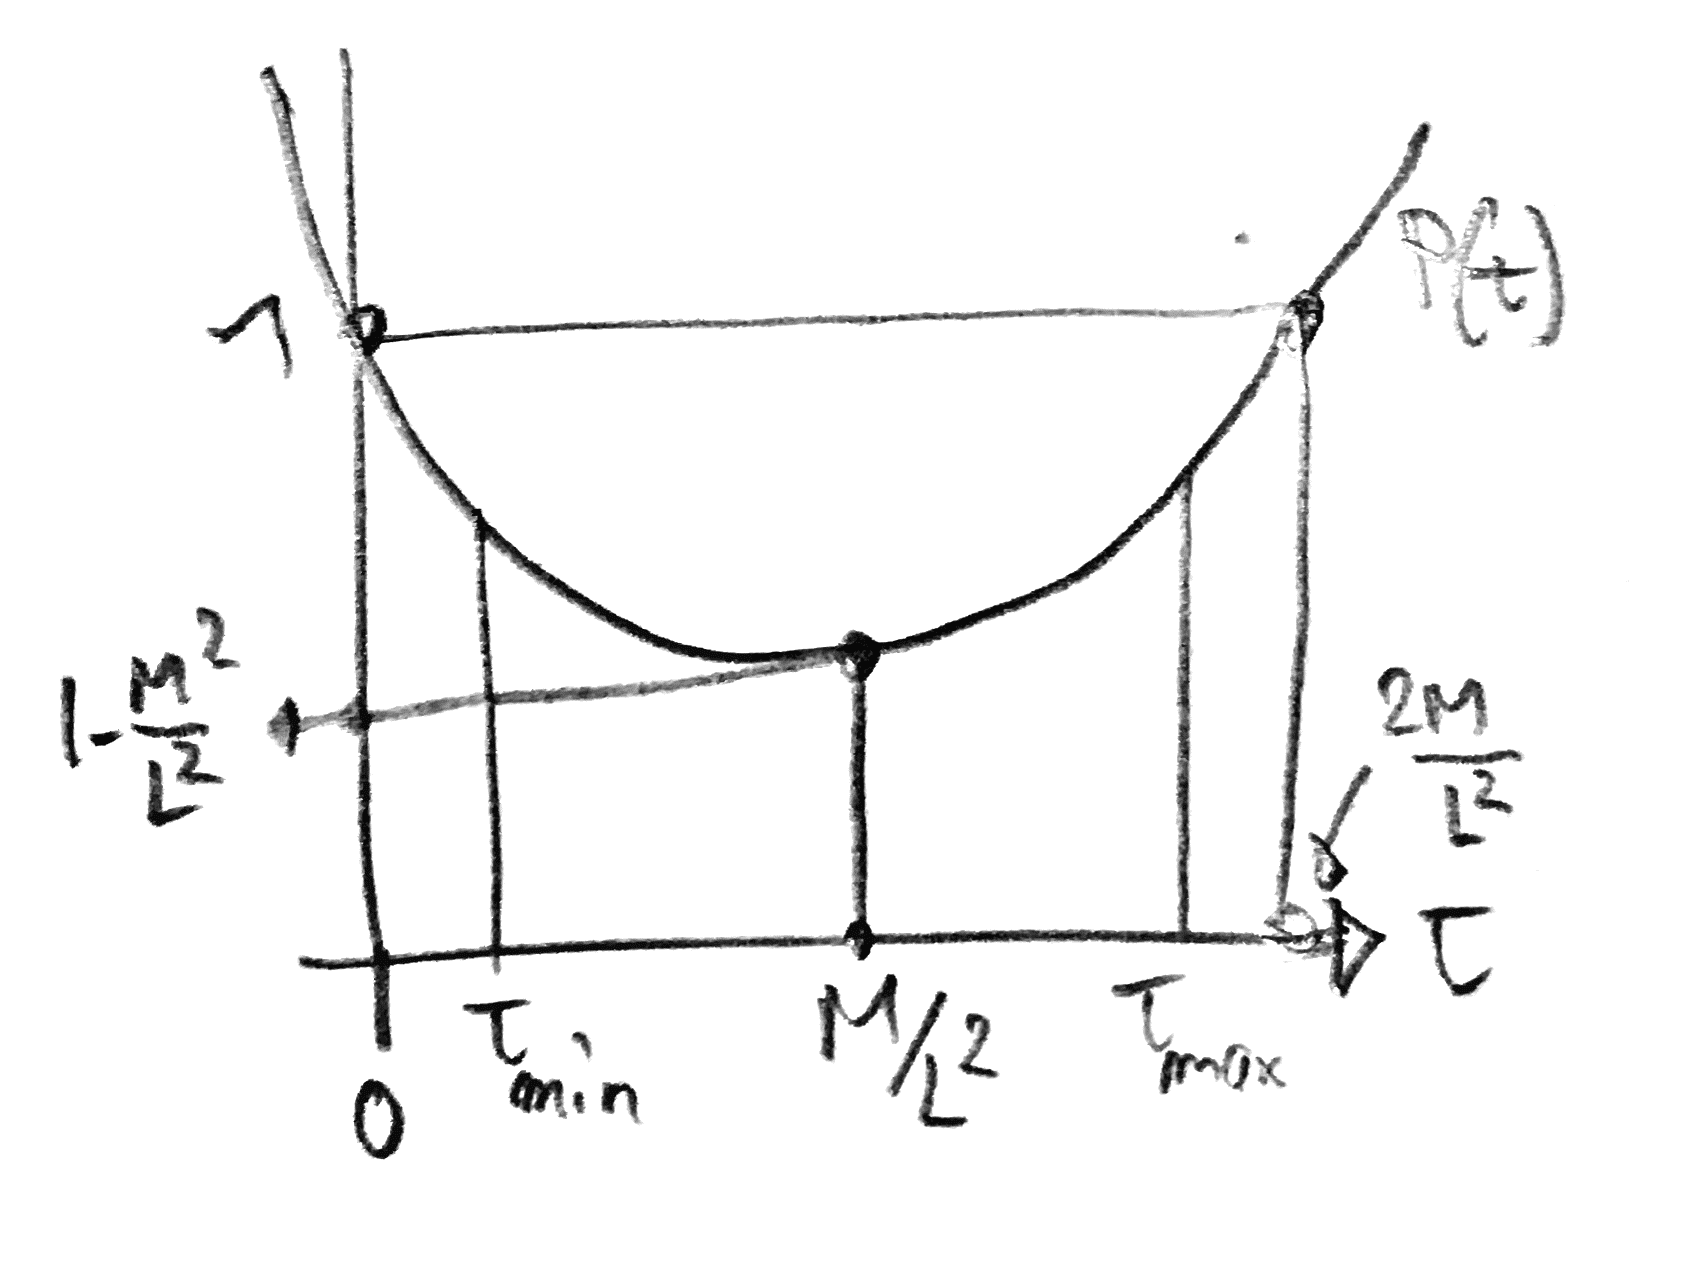
\includegraphics[width=.35\linewidth]{inverse-problems/grad-desc-general} \quad
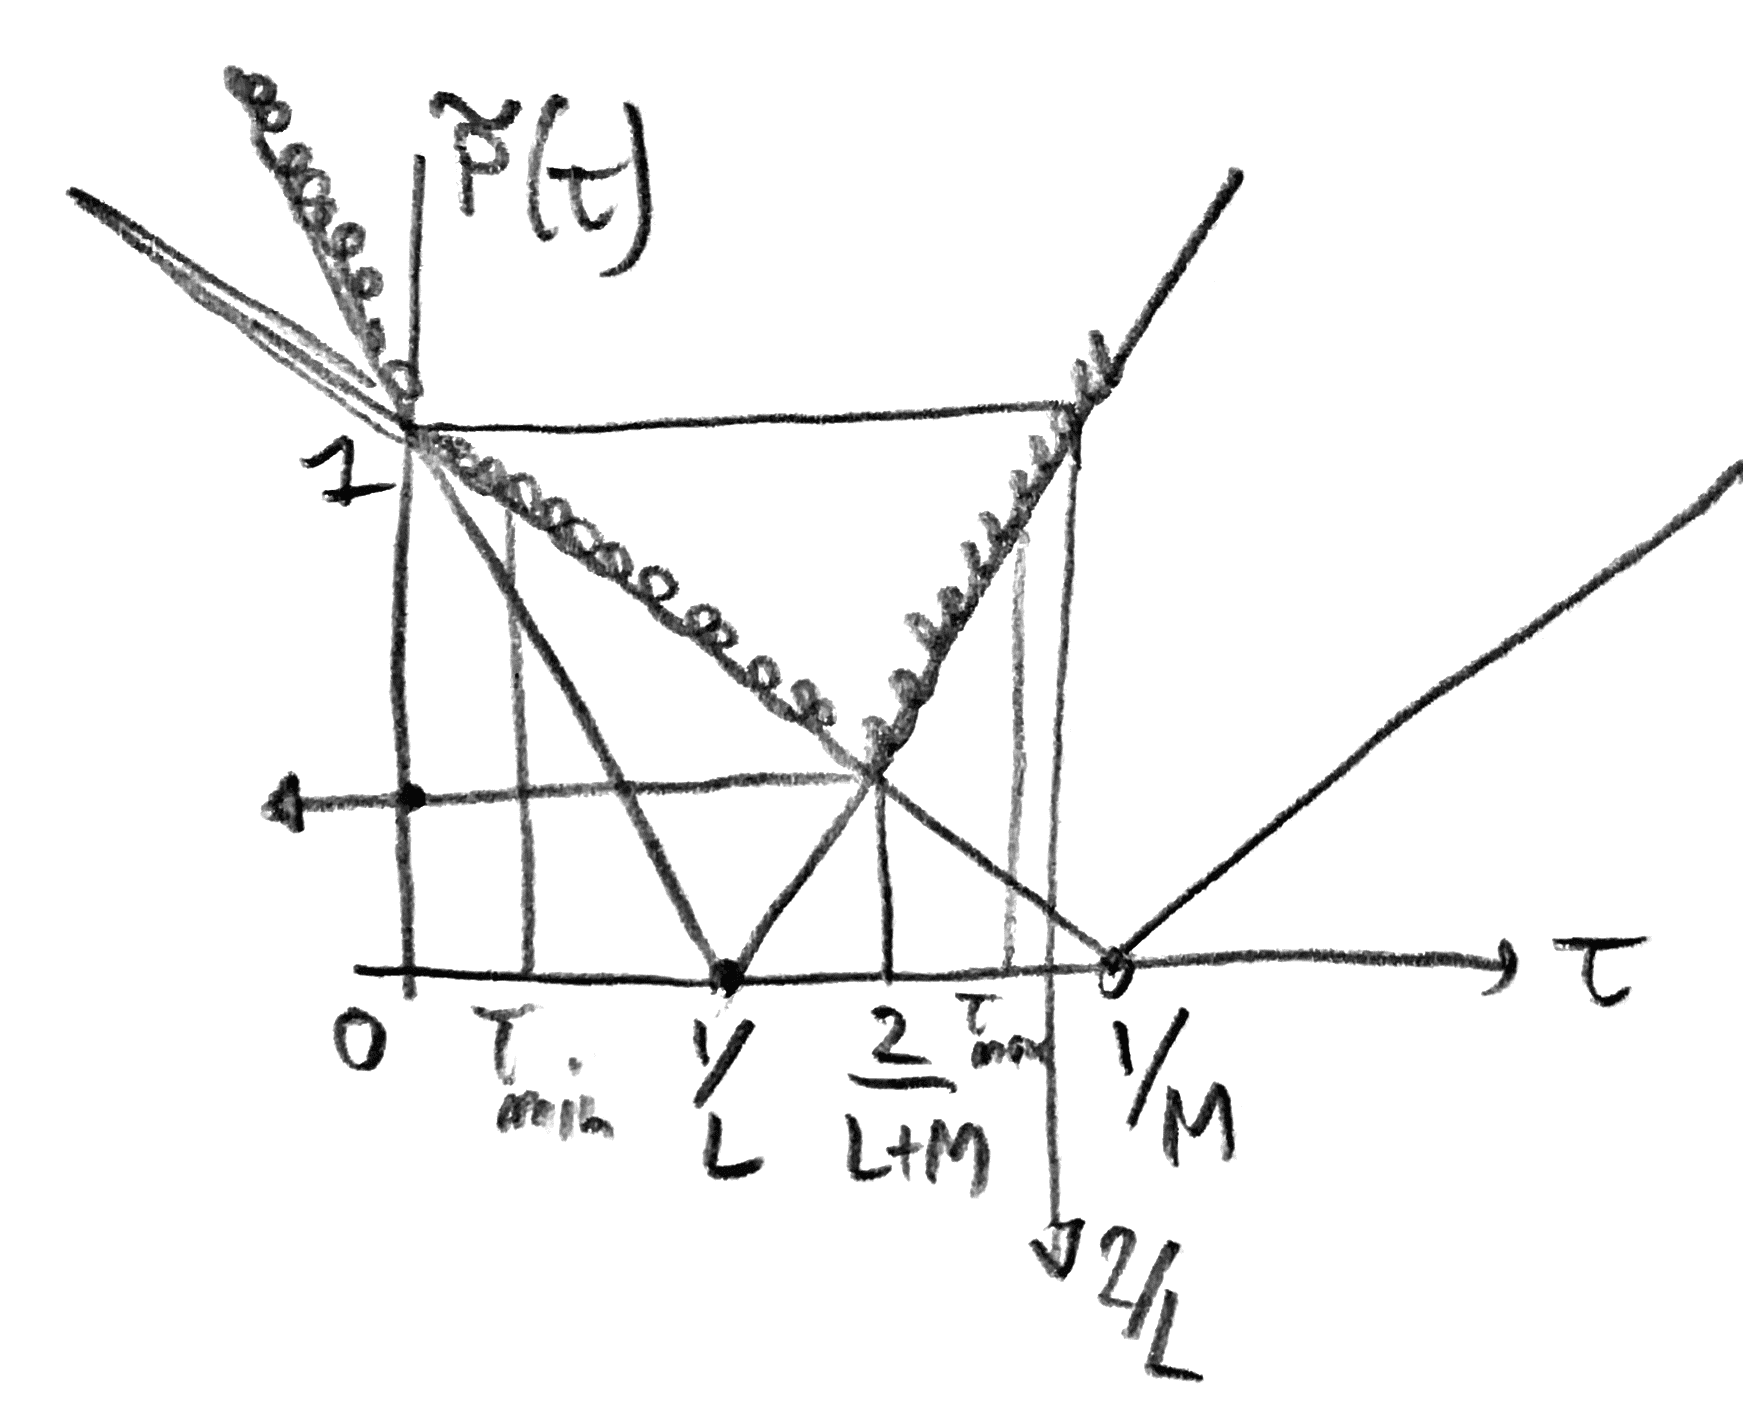
\includegraphics[width=.35\linewidth]{inverse-problems/grad-desc-linear}
\caption{\label{fig-grad-desc-contract}
Contraction constant $P(\tau)$ and $\tilde P(\tau)$ for a gradient descent step in the generic case (left) and for a quadratic function (right). 
}
\end{figure}

The error decay rate~\eqref{eq-global-linrate-grad}, although it is geometrical $O(\rho^\ell)$ is called a ``linear rate'' in the optimization literature. It is a ``global'' rate because it hold for all $\ell$ (and not only for large enough $\ell$).
%
The best (smallest) rate $\rho$ is obtained when choosing 
\eql{\label{eq-best-rate-global}
	\tau_\ell = \frac{\mu}{L^2}
	\qarrq
	\rho = 1 - \frac{\mu^2}{L^2}.
} 

In the case of a quadratic functional of the form~\eqref{eq-quad-func}, one can sharpen the convergence proof because the iterates are computed in closed form using matrix multiplication
\eq{
	\it{x}-x^\star = ( \Id_{N} - \tau_\ell A ) (\itz{x}-x^\star)
}
which leads to the following proposition (see also Figure~\ref{fig-grad-desc-contract}, right, for the corresponding contraction constant involved as a function of $\tau$).

\begin{prop}\label{prop-graddesc-quad}
	For $f(x)=\dotp{A}{f}-\dotp{b}{x}$ with the singular values of $A$ upper-bounded by $L$, assuming there exists $(\tau_{\min},\tau_{\max})$ such that
	\eql{\label{eq-descent-step-cond}
		0 < \tau_{\min} \leq \tau_\ell \leq \tilde\tau_{\max} < \frac{2}{L}
	}
	then there exists $0 \leq \tilde\rho<1$ such that 
	\eql{\label{eq-global-linrate-grad}
		\norm{ \it{x}-x^\star } \leq \tilde\rho^\ell \norm{\itz{x}-x^\star}.
	} 
	If the singular values are lower bounded by $\mu$, then the best rate $\tilde\rho$ is obtained for 
	\eql{\label{eq-best-rate-local}
		\tau_\ell = \frac{2}{L+\mu}
		\qarrq
		\tilde\rho \eqdef \frac{L-\mu}{L+\mu}.
	} 
\end{prop}


The maximum allowable step size $\tilde\tau_{\max}$ in~\eqref{eq-descent-step-cond} is much larger than $\tau_{\max}$ given in~\eqref{eq-descent-step-cond}, and the optimal rate~\eqref{eq-best-rate-local} is also much better (smaller) than the one in~\eqref{eq-best-rate-global}. In particular, if 
\eq{
	\epsilon \eqdef M/L \ll 1
} 
(which is the typical setup for ill-posed problems), then 
\eq{
	\rho \sim 1-\epsilon^2
	\qandq
	\tilde\rho \sim 1 - 2\epsilon.
}
The quantity $\epsilon$ in some sense reflects the inverse-conditioning of the problem. For quadratic function, it indeed corresponds exactly to the inverse of the condition number (which is the ratio of the largest to smallest singular value). The condition number is minimum and equal to $1$ for orthogonal matrices.

These two results are however complementary. Indeed, if the gradient descent converges, then ultimately $\it{x}$ is close to $x^\star$, so that one can approximate up to second order $f(x) \approx f(x^\star) + \dotp{Af}{f}-\dotp{f}{b}$ with $A=\partial^2 f(x^\star)$ and $b=-\nabla f(x^\star)$. So that the ``local'' rate, the one obtained after a large enough of iterations, is actually driven by $\tilde\rho$ and not $\rho$. It is thus important to distinguish between the global rate and the local rate. In practice, descent algorithm typically have two phase: a first ``slow'' phase govern by the global rate, and a second ``fast'' phase governed by the local rate. Unfortunately, the optimal step sizes $\tau_\ell$ are in general different for the two phase, so that optimal adaptation of step size is a difficult problems. This is why more advanced users typically use various line search strategies (to find the optimal step size at each iteration) or use second order information using quasi-Newton technics (BFGS).

The convergence result of Proposition~\ref{prop-graddesc-quad} does not requires strong convexity, while Theorem~\ref{thm-gradsec-strong-conv} does. In the general non-strongly convex case, it is still possible to prove convergence, but the rate is only sub-linear, and is only on the value of $f$, not on the iterate $\it{x}$ themselves.
%
Note that in this case, the solution of the minimization problem is not necessarily unique.
%
The proof is more technical.

\begin{thm}\label{thm-gradsec-non-strong-conv}
	If $f$ satisfy conditions~\eqref{eq-lipsch-grad}, assuming there exists $(\tau_{\min},\tau_{\max})$ such that
	\eql{\label{eq-descent-step-cond}
		0 < \tau_{\min} \leq \tau_\ell \leq \tau_{\max} < \frac{2}{L}, 
	}
	then $\it{x}$ converges to a solution $x^\star$ of~\eqref{eq-min-smooth-uncons} and
	there exists $C>0$ such that 
	\eql{\label{eq-sublin-rate-gd}
		f(\it{x})-f(x^\star) \leq \frac{C}{\ell+1}.
	} 
\end{thm}
\begin{proof}
	We only prove~\eqref{eq-sublin-rate-gd} since the proof that $\it{x}$ converges is more technical. Note indeed that if the minimizer $x^\star$ is non-unique, then it might be the case that the iterate $\it{x}$ ``cycle'' while approaching the set of minimizer, but actually convexity of $f$ prevents this kind of pathological behavior. 
	%
	For simplicity, we do the proof in the case $\tau_\ell = 1/L$, but it extends to the general case. 
	%
	The $L$-smoothness property imply~\eqref{eq-above-below-quad}, which reads
	\eq{
	f(\iit{x}) 
		\leq 
		f(\it{x}) + \dotp{\nabla f(\it{x})}{\iit{x}-\it{x}} + \frac{L}{2}\norm{\iit{x}-\it{x}}^2.
	}
	Using the fact that $\iit{x}-\it{x} = -\frac{2}{L} \nabla f(\it{x})$, one obtains
	\eql{\label{eq-proox-x'rad-nonstrong-1}
		f(\iit{x}) 
		\leq 
		f(\it{x}) -  \norm{\nabla f(\it{x})}^2
		\leq 
		f(\it{x}) - \frac{1}{2L} \norm{\nabla f(\it{x})}^2
	}
	This shows that $(f(\it{x}))_\ell$ is a decaying sequence.
	%
	By convexity
	\eq{
		f(\it{x}) + \dotp{\nabla f(\it{x})}{x^\star-\it{x}}�\leq  f(x^\star)
	}
	and plugging this in~\eqref{eq-proox-x'rad-nonstrong-1} shows
	\begin{align*}
		f(\iit{x})  &\leq   
		f(x^\star) - \dotp{\nabla f(\it{x})}{x^\star-\it{x}} - \frac{1}{2L} \norm{\nabla f(\it{x})}^2 \\
		&= f(x^\star) + \frac{L}{2}\pa{
			\norm{\it{x}-x^\star}^2 - \norm{\it{x}-x^\star-\frac{1}{L}\nabla f(\it{x})}^2
		}\\
		&= f(x^\star) + \frac{L}{2}\pa{
			\norm{\it{x}-x^\star}^2 - \norm{x^\star-\iit{x}}^2 }.
	\end{align*}
	Summing these inequalities for $\ell=0,\ldots,k$, one obtains
	\eq{
		\sum_{\ell=1}^k f(\iit{x}) - k x^\star \leq  \frac{L}{2}\pa{
			\norm{\itz{x}-x^\star}^2 - \norm{x^{(k+1)}-x^\star}^2 }
	}
	and since $f(\iit{x})$ is decaying $\sum_{\ell=1}^k f(\iit{x}) \geq (k+1) f(x^{(k+1)})$, thus 
	\eq{
		f(x^{(k+1)}) - f(x^\star) \leq \frac{L \norm{\itz{x}-x^\star}^2}{2(k+1)}
	}
	which gives~\eqref{eq-sublin-rate-gd} for $C \eqdef L \norm{\itz{x}-x^\star}^2/2$.
\end{proof}


%%%%%%%%%%%%%%%%%%%%%%%%%%%%%%%%%%%%%%%%%%%%%%%%
\subsection{Sub-gradient Descent}

The gradient descent~\eqref{eq-grad-desc} cannot be applied on a non-smooth function $f$. One can use in place of a gradient a sub-gradient, which defines the sub-gradient descent
\eql{\label{eq-subgrad-desc}
	\iit{x} \eqdef \it{x} - \tau_\ell \it{g}
	\qwhereq
	\it{g} \in \partial f( \it{x} ).
}
The main issue with this scheme is that to ensure convergence, the iterate should go to zero. One can easily convince oneself why by looking at the iterates on a function $f(x)=|x|$.

\begin{thm}
	If $\sum_{\ell} \tau_\ell=+\infty$ and $\sum_{\ell} \tau_\ell^2 < +\infty$, then $\it{x}$ converges to a minimizer of $f$. 
\end{thm}

%%%%%%%%%%%%%%%%%%%%%%%%%%%%%%%%%%%%%%%%%%%%%%%%%%%%%%%%%%%%%%%%%%%%%%%%%%%%%%%%%%
\subsection{Projected Gradient Descent}
\label{sec-proj-grad}

We consider a generic constraint optimization problem as
\eql{\label{eq-constr}
	\umin{x \in \Cc} f(x) 
} 
where $\Cc \subset \RR^S$ is a closed convex set and $f : \RR^S \rightarrow \RR$ is a smooth convex function (at least of class $\Cc^1$). 

The gradient descent algorithm~\eqref{eq-grad-desc}�is generalized to solve a constrained problem using the projected gradient descent 
\eql{\label{eq-proj-grad-desc}
	\iit{x} \eqdef \Proj_\Cc \pa{ \it{x} - \tau_\ell \nabla f( \it{x} ) }, 
}
where $\Proj_\Cc$ is the orthogonal projector on $\Cc$
\eq{
	\Proj_\Cc(x) = \uargmin{x' \in \Cc} \norm{x-x'}
}
which is always uniquely defined because $\Cc$ is closed and convex.
%
The following proposition shows that all the convergence properties of the classical gradient descent caries over to this projected algorithm.

\begin{thm}\label{thm-proj-grad}
	Theorems~\ref{thm-gradsec-strong-conv} and~\ref{thm-gradsec-non-strong-conv} still holds when replacing iterations~\eqref{eq-grad-desc} by~\eqref{eq-proj-grad-desc}.
\end{thm}

\begin{proof}
	The proof of Theorem~\ref{thm-gradsec-strong-conv} extends because the projector is contractant, 
	$\norm{\Proj_\Cc(x)-\Proj_\Cc(x')} \leq \norm{x-x'}$ so that the strict contraction properties of the gradient descent is maintained by this projection.   
\end{proof}

The main bottleneck that often prevents to use~\eqref{eq-proj-grad-desc} is that the projector is often complicated to compute. We are however lucky since for $\ell^1$ mininization, one can apply in a straightforward manner this method. 





%%%%%%%%%%%%%%%%%%%%%%%%%%%%%%%%%%%%%%%%%%%%%%%%%%%%%%%%%%%%%%%%%%%%%%%%%%%%%%%%%%
%%%%%%%%%%%%%%%%%%%%%%%%%%%%%%%%%%%%%%%%%%%%%%%%%%%%%%%%%%%%%%%%%%%%%%%%%%%%%%%%%%
%%%%%%%%%%%%%%%%%%%%%%%%%%%%%%%%%%%%%%%%%%%%%%%%%%%%%%%%%%%%%%%%%%%%%%%%%%%%%%%%%%
\section{Proximal Operators}

For non-smooth functions $f$, it is not possible to perform an ``explicit'' gradient descent step because the gradient is not even defined. One thus needs to replace this ``explicit''  step by an ``implicit'' one, which is possible even if $f$ is non-smooth.


%%%%%%%%%%%%%%%%%%%%%%%%%%%%%%%%%%%%%%%%%%%%%%%%
\subsection{Proximal Map }

The implicit stepping of amplitude $\tau>0$ is defined as 
\eql{\label{eq-defn-proximal}
	\foralls x, \quad
	\Prox_{\tau f}(x) \eqdef \uargmin{x'} \frac{1}{2}\norm{x-x'}^2 + f(x').
}
It amounts to minimize function $f$ locally around $x$, in a ball of radius controlled by $\tau$.
%
This the involved function $\frac{1}{2}\norm{x-\cdot}^2 + f$ is strongly convex, this operator $\Prox_{\tau f}$ is well defined and single-valued. 

When $f=\iota_\Cc$ is an indicator, the proximal map boils down to a projection $\Prox_{\iota_\Cc}=\Proj_{\Cc}$, it is thus in some sense a generalization of the projection to arbitrary function. And can also be interpreted as a projector on a level set of $f$. 

%%%
\paragraph{Examples}


As  simple examples, let us list
\eq{
	\Prox_{\frac{\tau}{2} \norm{\cdot}^2}(x) =  \frac{x}{1+\tau}, 
	\qandq
	\Prox_{\tau \norm{\cdot}_1} = \Ss_\tau^1(x), 
}
where the soft-thresholding is defined as
\eq{
	\Ss_\tau^1(x) = ( S_\tau(x_i) )_{i=1}^N \qwhereq
	S_\tau(r) = \sign(r) (|r|-\la)_+, 
}
(see also~\eqref{eq-soft-thresh}).

Note that in some case, the proximal map of a non-convex function is well defined, for instance
$\Prox_{\tau \norm{\cdot}_0}$ is the hard thresholding associated to the threshold $\sqrt{2\tau}$, see Proposition~\ref{prop-equiv-sparse-thresh}.


%%%
\paragraph{Basic properties.}

If $f(x)=\sum_{k=1}^K f(x_k)$ for $x=(x_1,\ldots,x_K)$ is separable, then
\eq{
	\Prox_{\tau f}(x) = ( \Prox_{\tau f_k}(x_k) )_{k=1}^K.
}
The following proposition is very useful.

\begin{prop}
	If $A \in \RR^{P \times N}$ is a tight frame, i.e. $AA^*=\Id_P$, then 
	\eq{
		\Prox_{f \circ A} = A^* \circ \Prox_{f} \circ A + \Id_N - A^* A.
	}
	In particular, if $A$ is orthogonal, then $\Prox_{f \circ A} = A^* \circ \Prox_{f} \circ A$.
\end{prop}

%%%
\paragraph{Link with sub-differential.}

For a set-valued map $U : \Hh \hookrightarrow \Gg$, we define the inverse set-valued map $U^{-1} : \Gg \hookrightarrow \Hh$ by 
\eq{
	h \in U^{-1}(g) 
	\quad\Longleftrightarrow\quad
	g \in U(h) 
} 

% TODO: add picture

One has the following equivalence
\eq{
	z = \Prox_{\tau f}(x) 
	\Leftrightarrow
	0 \in z-x+\tau\partial f(z)
	\Leftrightarrow
	x \in (\Id+\tau\partial f)(z)
	\Leftrightarrow
	z = (\Id+\tau\partial f)^{-1}(x)
}	
where for the last equivalence, we have replace ``$\in$'' by ``$=$'' because the proximal map is single valued.
%
The proximal operator is hence often referred to the ``resolvent'' $\Prox_{\tau f} = (\Id+\tau\partial f)^{-1}$ of the maximal monotone operator $\partial f$. 
% 


%%%%%%%%%%%%%%%%%%%%%%%%%%%%%%%%%%%%%%%%%%%%%%%%
\subsection{Proximal Point Algorithm}

One has the following equivalence 
\begin{align}\label{eq-proxpoint-fix}
	x^\star \in \argmin f
	&\quad\Leftrightarrow\quad
	0 \in \partial f(x^\star)
	\quad\Leftrightarrow\quad
	x^\star \in (\Id+\tau \partial f)(x^\star) \\
	&\quad\Leftrightarrow\quad
	x^\star = (\Id+\tau \partial f)^{-1}(x^\star) = \Prox_{\tau f}(x^\star).
\end{align}
This shows that being a minimizer of $f$ is equivalent to being a fixed point of $\Prox_{\tau f}$.
%
This suggest the following fixed point iterations, which are called the proximal point algorithm 
\eql{\label{eq-proximal-point}
	\iit{x} \eqdef \Prox_{\tau_\ell f}(\it{x}).
}
On contrast to the gradient descent fixed point scheme, the proximal point method is converging for any sequence of steps.

\begin{thm}
	If $0<\tau_{\min} \leq \tau_\ell \leq \ga_{\max} < +\infty$, then $\it{x} \rightarrow x^\star$ a minimizer of $f$.
\end{thm}

This implicit step~\eqref{eq-proximal-point} should be compared with a gradient descent step~\eqref{eq-grad-desc}
\eq{
	\iit{x} \eqdef (\Id+\tau_\ell \nabla f)(\it{x}).
}
One sees that the implicit resolvent $(\Id-\tau_\ell \partial f)^{-1}$ replaces the explicit step $\Id+\tau_\ell \nabla f$. For small $\tau_\ell$ and smooth $f$, they are equivalent at first order. But the implicit step is well defined even for non-smooth function, and the scheme (the proximal point) is always convergent (whereas the explicit step size should be small enough for the gradient descent to converge). This is inline with the general idea the implicit stepping (e.g. implicit Euler for integrating ODE, which is very similar to the proximal point method) is more stable. Of course, the drawback is that explicit step are very easy to implement whereas in general proximal map are hard to solve (most of the time as hard as solving the initial problem).


%%%%%%%%%%%%%%%%%%%%%%%%%%%%%%%%%%%%%%%%%%%%%%%%
\subsection{Forward-Backward}
\label{sec-fb}

It is in general impossible to compute $\Prox_{\ga f}$ so that the proximal point algorithm is not implementable.
%
In oder to derive more practical algorithms, it is important to restrict the class of considered function, by imposing some structure on $f$. We consider functions of the form
\eql{\label{eq-fb-split}
	f(x) =  \Ff(x) +  \Gg(x)
}
where $\Gg \in \Ga_0(\Hh)$ can be an arbitrary, but $\Ff$ needs to be smooth.

One can modify the fixe point derivation~\eqref{eq-proxpoint-fix} to account for this special structure
\begin{align*}
 	x^\star \in \argmin \Ff + \Gg
	& \quad\Leftrightarrow\quad
	0 \in \nabla \Ff(x^\star) + \partial \Gg(x^\star) 
	\quad\Leftrightarrow\quad
	x^\star - \tau \nabla \Ff(x^\star) \in (\Id+\tau \partial \Gg)(x^\star) \\
	& \quad\Leftrightarrow\quad
	x^\star = ( \Id + \tau \partial \Gg )^{-1} \circ ( \Id - \tau \nabla \Ff ) (x^\star).
\end{align*}
This fixed point suggests the following algorithm, with the celebrated Forward-Backward
\eql{\label{eq-fb}
		\iit{x} \eqdef \Prox_{\tau_\ell \Gg}\pa{ \it{x} - \tau_\ell \nabla\Ff(\it{x}) }.
}


%%%
\paragraph{Derivation using surrogate functionals.}

An intuitive way to derive this algorithm, and also a way to prove its convergence, it using the concept of surrogate functional.

%
% The difficulty is the presence of the operator $A$ in the $\ldeux$ norm, which makes this problem significantly more difficult than the simple denoising by regularization\eqref{eq-regul-denoising}.

To derive an iterative algorithm, we modify the energy $f(x)$ to obtain a surrogate functional $f(x,\it{x})$ whose minimization corresponds to a simpler optimization problem, and define the iterations as
\eql{\label{eq-surrogate-iter}
	\iit{x} \eqdef \uargmin{x} f(x,\it{x}).
}
In order to ensure convergence, this function should satisfy the following property
\eql{\label{eq-surrogate-pty}
	f(x) \leq f(x,x')
	\qandq
	f(x,x) = f(x)
}
and $f(x)-f(x,x')$ should be a smooth function.
%
Property \eqref{eq-surrogate-pty} guarantees that $f$ is decaying by the iterations
\eq{
	f(\iit{x}) \leq f(\it{x})
}
and it simple to check that actually all accumulation points of $(\it{x})_\ell$ are stationary points of $f$. 

In order to derive a valid surrogate $f(x,x')$ for our functional~\eqref{eq-fb-split}, since we assume $\Ff$ is $L$-smooth (i.e. satisfies~\eqref{eq-lipsch-grad}), let us recall the quadratic majorant~\eqref{eq-above-below-quad}
\eq{
	\Ff(x) 
	\leq 
	\Ff(x') + \dotp{\nabla \Ff(x')}{x'-x} + \frac{L}{2}\norm{x-x'}^2, 
}
so that for $0 < \tau < \frac{1}{L}$, the function 
\eql{\label{eq-surrogate-ip}
	f(x,x') \eqdef \Ff(x') + \dotp{\nabla \Ff(x')}{x'-x} + \frac{1}{2\tau}\norm{x-x'}^2 + \Gg(x)
}
satisfies the surrogate conditions~\eqref{eq-surrogate-pty}.
%
The following proposition shows that minimizing the surrogate functional corresponds to the computation of a so-called proximal operator. 

\begin{prop}
	The update~\eqref{eq-surrogate-iter} for the surrogate~\eqref{eq-surrogate-ip} is exactly~\eqref{eq-fb}.
\end{prop}
\begin{proof}
	This follows from the fact that
	\eq{
		\dotp{\nabla \Ff(x')}{x'-x} + \frac{1}{2\tau}\norm{x-x'}^2 
		= \frac{1}{2\tau} \norm{ x - (x'-\tau \nabla\Ff(x'))  }^2 + \text{cst}.
	}
\end{proof}

%%%
\paragraph{Convergence of FB. }

Although we impose $\tau<1/L$ to ensure majorization property, one can actually show convergence under the same hypothesis as for the gradient descent, i.e. $0 < \tau < 2/L$, with the same convergence rates.  This means that Theorem~\ref{thm-proj-grad} for the projected gradient descent extend to FB. 

\begin{thm}\label{thm-fb-conv}
	Theorems~\ref{thm-gradsec-strong-conv} and~\ref{thm-gradsec-non-strong-conv} still holds when replacing iterations~\eqref{eq-grad-desc} by~\eqref{eq-fb}.
\end{thm}

Note furthermore that the projected gradient descent algorithm~\eqref{eq-proj-grad-desc} is recovered as a special case of~\eqref{eq-fb} when setting $J=\iota_{\Cc}$ the indicator of the constraint set, since $\Prox_{\rho J} = \Proj_{\Cc}$ in this case.

Of course the difficult point is to be able to compute in closed form $\Prox_{\tau \Gg}$ in~\eqref{eq-fb}, and this is usually possible only for very simple function. We have already seen such an example in Section~\ref{sec-ista} for the resolution of $\ell^1$-regularized inverse problems (the Lasso).


%%%%%%%%%%%%%%%%%%%%%%%%%%%%%%%%%%%%%%%%%%%%%%%%%%%%%%%%%%%%%%%%%%%%%%%%%%%%%%%%%%
%%%%%%%%%%%%%%%%%%%%%%%%%%%%%%%%%%%%%%%%%%%%%%%%%%%%%%%%%%%%%%%%%%%%%%%%%%%%%%%%%%
%%%%%%%%%%%%%%%%%%%%%%%%%%%%%%%%%%%%%%%%%%%%%%%%%%%%%%%%%%%%%%%%%%%%%%%%%%%%%%%%%%
\section{Primal-Dual Algorithms}

%%%%%%%%%%%%%%%%%%%%%%%%%%%%%%%%%%%%%%%%%%%%%%%%
\subsection{Forward-backward on the Dual}
\label{sec-fb-dual}

\paragraph{Chambolle's algorithm.}

Chambolle in \cite{chambolle-algo-tv}�detail an algorithm to minimize exactly the TV denoising problem
\eql{\label{eq-prox-tv}
	x_\la^\star = \uargmin{x \in \Hh} \frac{1}{2} \norm{x-x'}^2 + \la \normTV{x}.
}
It uses a relationship between the vectorial $\lun$ and $\linf$ norms
\eq{
	\normu{v} = \sum_{m=0}^{N-1} \norm{v_m} \qandq
	\normi{v} = \umax{0 \leq m < N} \norm{v_m}
}
where each $v_m \in \RR^2$ and $v \in \RR^{N \times 2}$. One has
\eq{
	\normu{v} = \umax{ \normi{w} \leq 1 } \dotp{w}{u}
}
which allows one to re-write the optimization \eqref{eq-prox-tv} as
\eq{
	\umin{x \in \Hh} \umax{\normi{w} \leq 1} 
		\frac{1}{2} \norm{x-x'}^2 + \la \dotp{w}{\nabla g}.
}
Exchanging the roles of the min and the max, one proves that the solution of  \eqref{eq-prox-tv} is re-written as
\eql{\label{eq-primal-dual-chambolle}
	x_\la^\star =  x + \la \diverg(w^\star)
}
where 
\eql{\label{eq-chambolle-dual}
	w^\star \in \uargmin{\normi{w} \leq 1} \norm{f + \la \diverg(w^\star)}^2.
}
The convex optimization problem \eqref{eq-chambolle-dual} computes a dual vector field $w^\star \in \RR^{N \times 2}$, from which the denoised image is recovered using \eqref{eq-primal-dual-chambolle}.

The dual problem \eqref{eq-chambolle-dual} is the minimization of a quadratic functional subject to a convex $\linf$ constraint. It can thus be solved using for instance a projected gradient descent
\eq{
	w^{(k+1)}_m = \frac{ \tilde w^{(k)}_m }{ \max(|\tilde w^{(k)}_m|,1) }
	\qwhereq
	\tilde w^{(k)} = w^{(k)} + \tau \nabla( f/\la + \diverg(w^{(k)}) ).
}  
If the gradient step size satisfy $0 < \tau < 1/4$, one can prove that 
\eq{
	f + \la \diverg(w^{(k)}) \longrightarrow f_\la^\star
	\qwhenq
	k \rightarrow +\infty.
}


%%%%%%%%%%%%%%%%%%%%%%%%%%%%%%%%%%%%%%%%%%%%%%%%
\subsection{Douglas-Rachford}


%%%%%%%%%%%%%%%%%%%%%%%%%%%%%%%%%%%%%%%%%%%%%%%%
\subsection{Primal-Dual Splitting}



% !TEX root = ../FundationsDataScience.tex

\chapter{Theory of Sparse Regularization}

We now apply the basics elements of convex analysis from the previous chapter to perform a theoretical analysis of the properties of the Lasso, in particular its performances to recover sparse vectors.





%%%%%%%%%%%%%%%%%%%%%%%%%%%%%%%%%%%%%%%%%%%%%%%%%%%%%%%%%%%%%%%%%%%%%%%%%%%%%%%%%%
%%%%%%%%%%%%%%%%%%%%%%%%%%%%%%%%%%%%%%%%%%%%%%%%%%%%%%%%%%%%%%%%%%%%%%%%%%%%%%%%%%
%%%%%%%%%%%%%%%%%%%%%%%%%%%%%%%%%%%%%%%%%%%%%%%%%%%%%%%%%%%%%%%%%%%%%%%%%%%%%%%%%%
\section{Existence and Uniqueness}


%%%%%%%%%%%%%%%%%%%%%%%%%%%%%%%%%%%%%%%%%%%%%%%%%%%%%%%%%%%%%%%%%%%%%%%%%%%%%%%%%%
\subsection{Existence}

We consider problems~\eqref{eq-lasso-lagr-ip} and~\eqref{eq-lasso-constr-ip}, that we rewrite here as 
\eql{\label{eq-lasso-lagr}\tag{$\Pp_\la(y)$}
	\umin{x \in \RR^N} f_\la(x) \eqdef \frac{1}{2\la} \norm{y-Ax}^2 + \la \norm{x}_1
} 
and its limit as $\la \rightarrow 0$
\eql{\label{eq-lasso-constr}\tag{$\Pp_0(y)$}
	\umin{A x = y} \norm{x}_1
	= \umin{x} f_0(x) \eqdef \iota_{\Ll_y}(x) + \norm{x}_1.
} 
where $A \in \RR^{P \times N}$, and $\Ll_y \eqdef \enscond{x \in \RR^N}{Ax=y}$.

We recall that the setup is that one observe noise measures
\eq{
	y=A x_0 + w
}
and we would like conditions to ensure for $x_0$ to solution to $(\Pp_0(Ax_0))$ (i.e. when $w=0$) and to be close (in some sense to be defined, and in some proportion to the noise level $\norm{w}$) to the solutions of $(\Pp_0(y=Ax_0+w))$ when $\la$ is wisely chosen as a function of $\norm{w}$. 

First let us note that since~\eqref{eq-lasso-lagr} is unconstrained and coercive (because $\norm{\cdot}_1$ is), this problem always has solutions.
%
Since $A$ might have a kernel and $\norm{\cdot}_1$ is not strongly convex, it might have non-unique solutions.
%
If $y \in \Im(A)$, the constraint set of~\eqref{eq-lasso-constr} is non-empty, and it also has solutions, which might fail to be unique.



\begin{figure}
\centering
%%
\begin{tabular}{@{}c@{}c@{}}
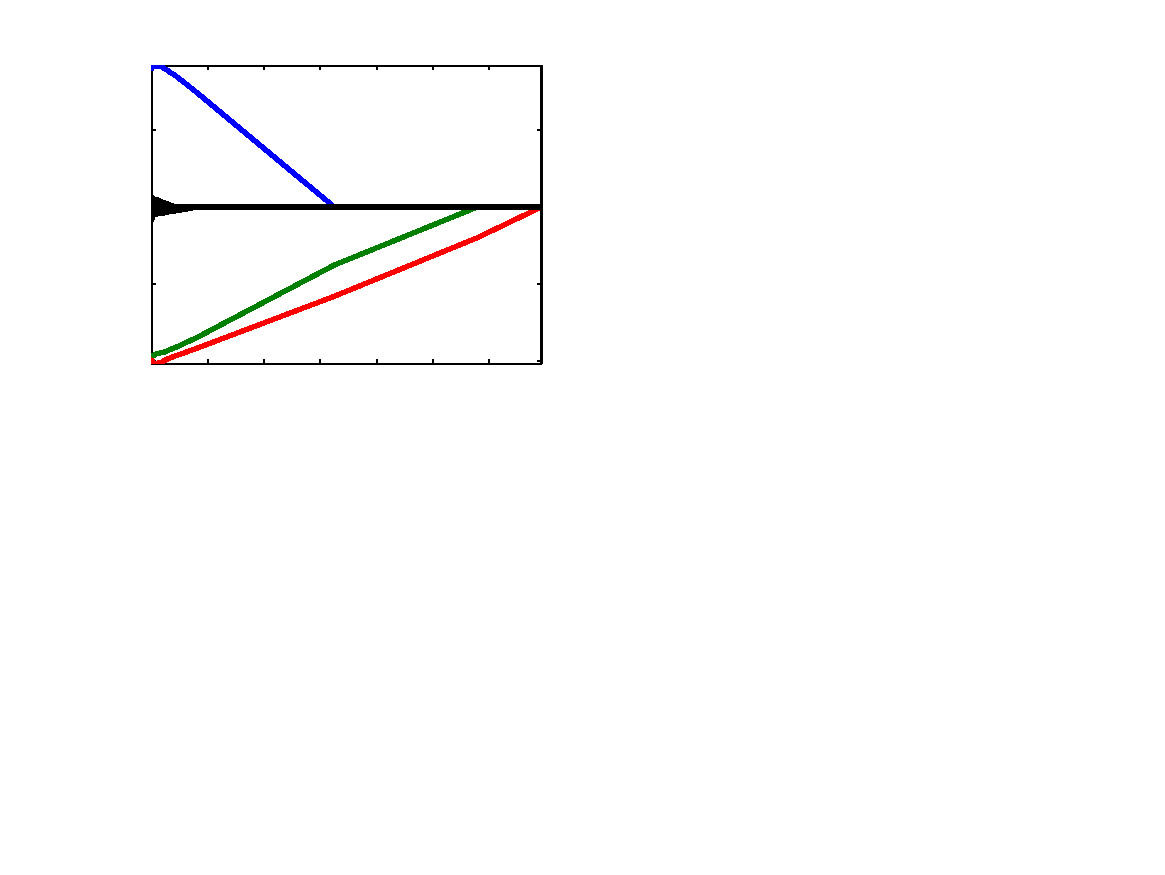
\includegraphics[width=.35\linewidth]{sparse-theory/homotopy/homotopy-s3}&
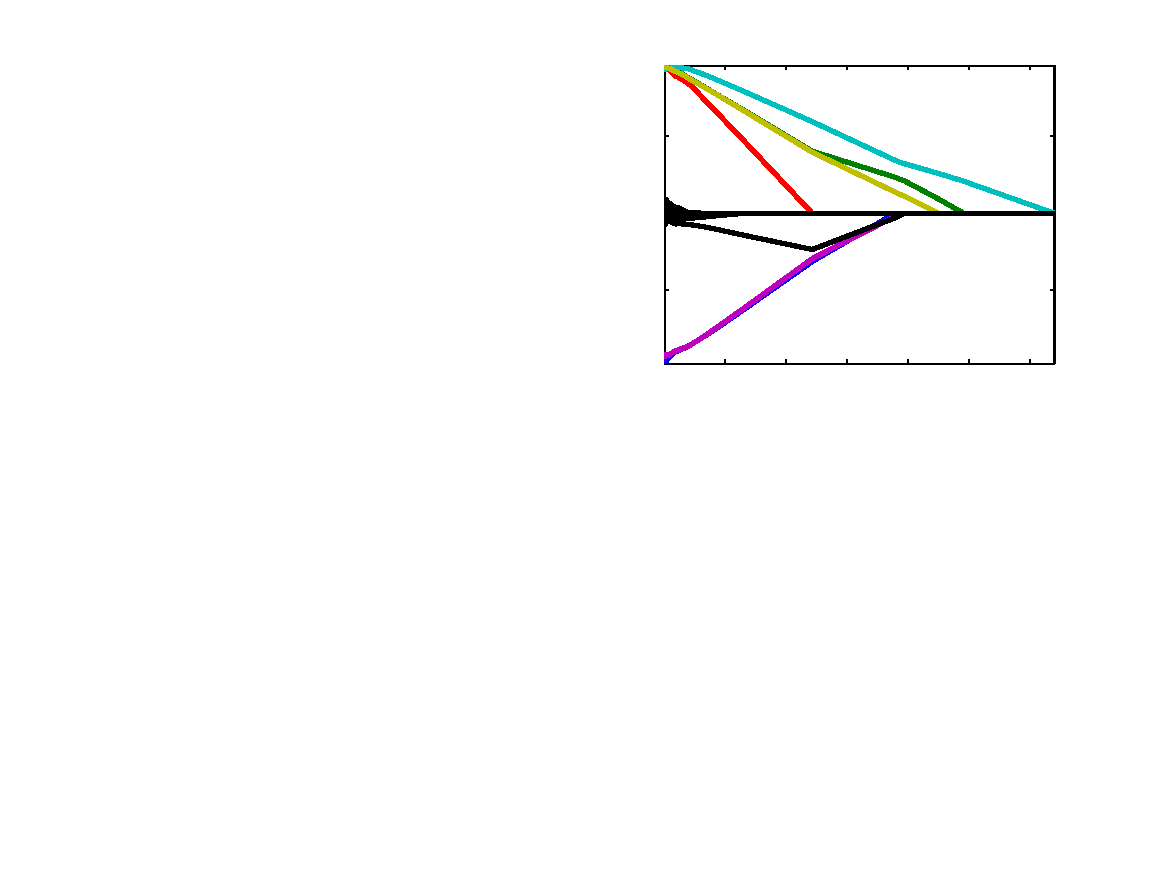
\includegraphics[width=.35\linewidth]{sparse-theory/homotopy/homotopy-s6}\\
$s=3$  & $s=6$ \\
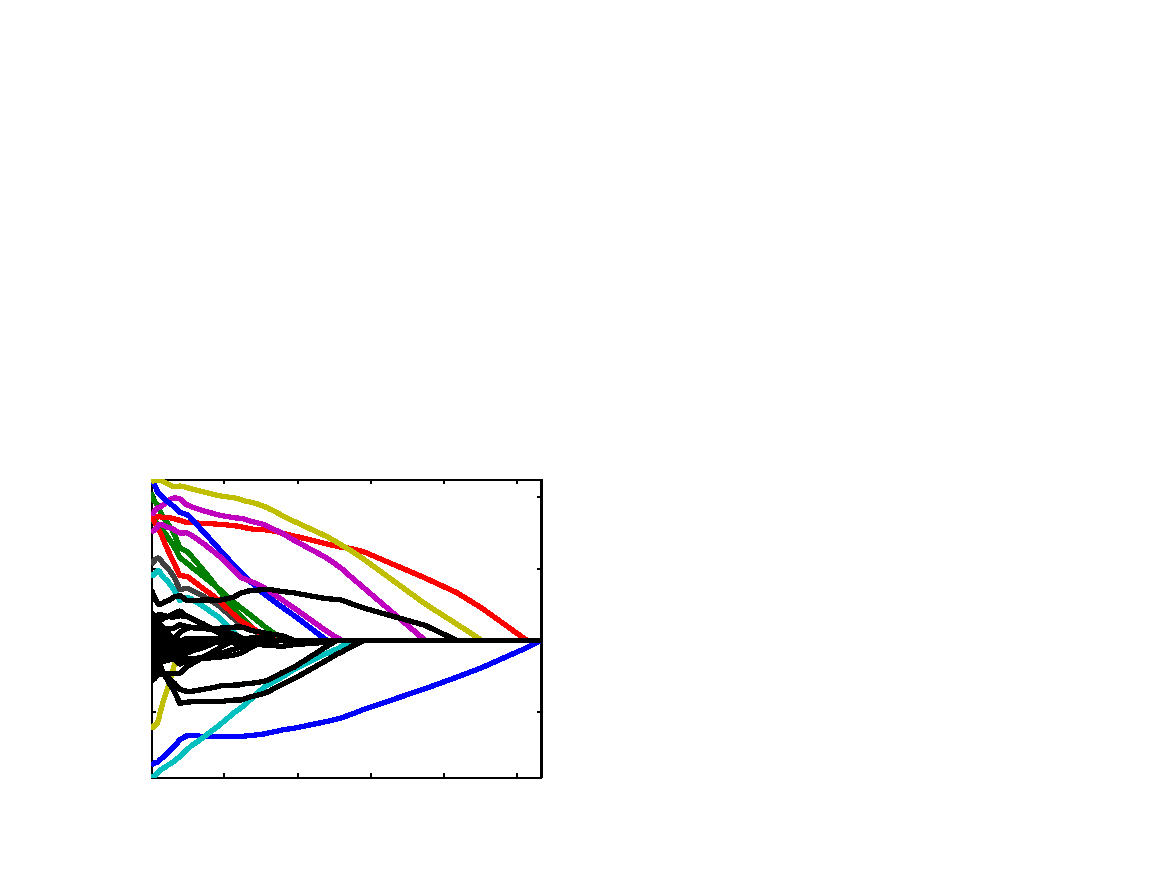
\includegraphics[width=.35\linewidth]{sparse-theory/homotopy/homotopy-s13}&
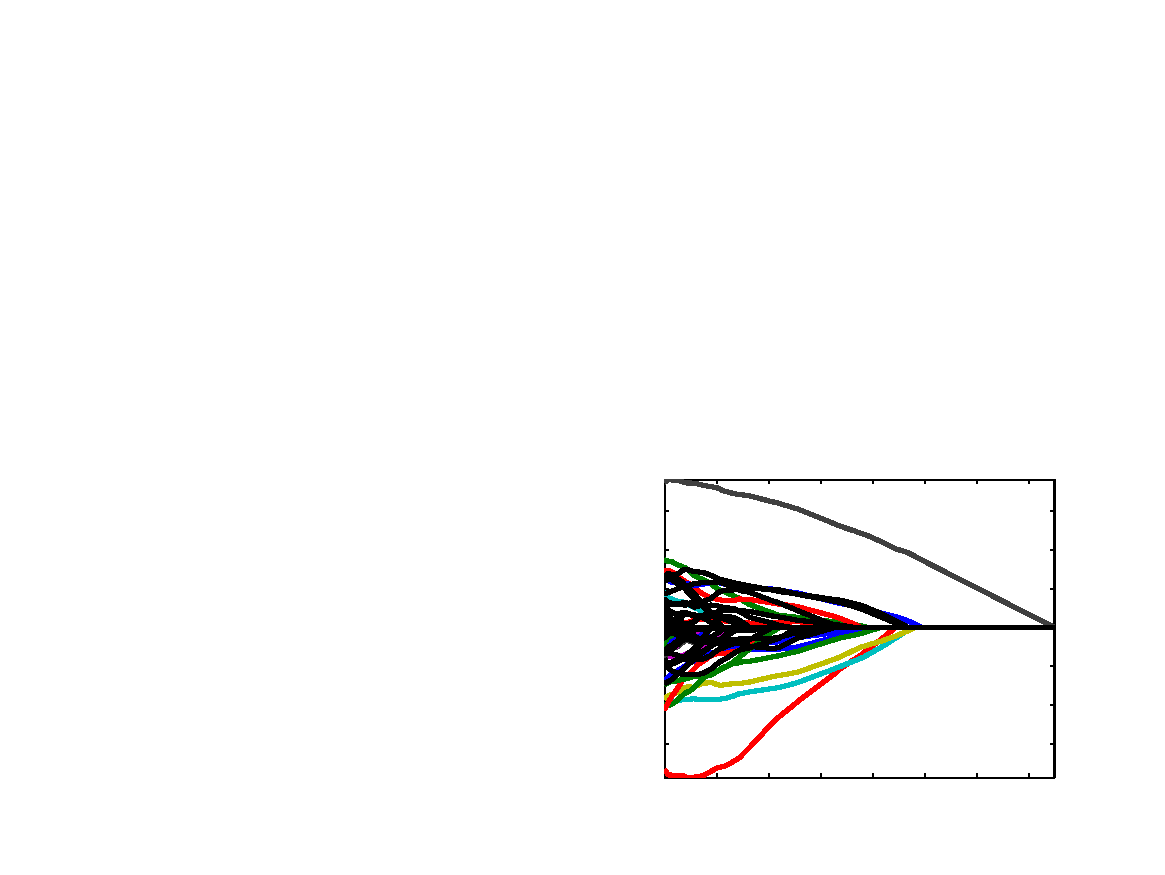
\includegraphics[width=.35\linewidth]{sparse-theory/homotopy/homotopy-s25}\\
$s=13$  & $s=25$ 
\end{tabular}
%%
\caption{\label{fig-homotopy}
Display of the evolution $\la \mapsto x_\la$ of the solutions of~\eqref{eq-lasso-lagr}.
}
\end{figure}

Figure~\ref{fig-homotopy} gives the intuition of the theory that will be developed in this chapter, regarding the exact or approximated recovery of sparse vectors $x_0$, and the need for a careful selection of the $\la$ parameter.





%%%%%%%%%%%%%%%%%%%%%%%%%%%%%%%%%%%%%%%%%%%%%%%%%%%%%%%%%%%%%%%%%%%%%%%%%%%%%%%%%%
\subsection{Polytope Projection for the Constraint Problem}
\label{sec-polytope-proj}

The following proposition gives a geometric description of those vectors which are recovered by $\ell^1$ minimization when there is no noise. 

\begin{prop}\label{prop-polytope-proj}
	We denote $B \eqdef \enscond{x \in \RR^N}{\norm{x}_1 \leq 1}$. Then, assuming $\Im(A)=\RR^P$, 
	\eql{\label{eq-polytop-ident} 
		x_0 \text{ is a solution to } \Pp_0(Ax_0)
		\quad\Longleftrightarrow\quad
		A \frac{x_0}{\norm{x_0}_1} \in \partial (AB)
	} 
	where ``$\partial$'' denoted the boundary and $AB=\enscond{Ax}{x\in B}$.
\end{prop}

\begin{proof}
	We first prove $``\Rightarrow''$. We suppose that $x_0$ is not a solution, and aim at showing that $A \frac{x_0}{\norm{x_0}_1} \in \text{int}(AB_\rho)$. Since it is not a solution, there exists $z$ such that $Ax_0=Az$ and $\norm{z}_1 = (1-\de)\norm{x_0}_1$ with $\de>0$. Then for any displacement $h=A\epsilon \in \Im(A)$, where one can impose $\epsilon \in \ker(A)^\bot$, i.e. $\epsilon=A^+h$, one has $Ax_0+h=A(z+\epsilon)$ and
	\eq{
		\norm{z+\epsilon}_1 \leq \norm{z}_1 + \norm{\Phi^+ h} \leq (1-\de) \norm{x_0}_1 + \norm{\Phi^+}_{1,1} \norm{h}_1 < \frac{\de}{\norm{A^+}_{1,1}}\norm{x_0}.
	}
	This means that choosing $\norm{h}_1 < \frac{\de}{\norm{A^+}_{1,1}} \norm{x_0}_1$ implies that $A \frac{x_0}{\norm{x_0}_1} \in \text{int}(AB)$.
	
\begin{figure}
\centering
%%
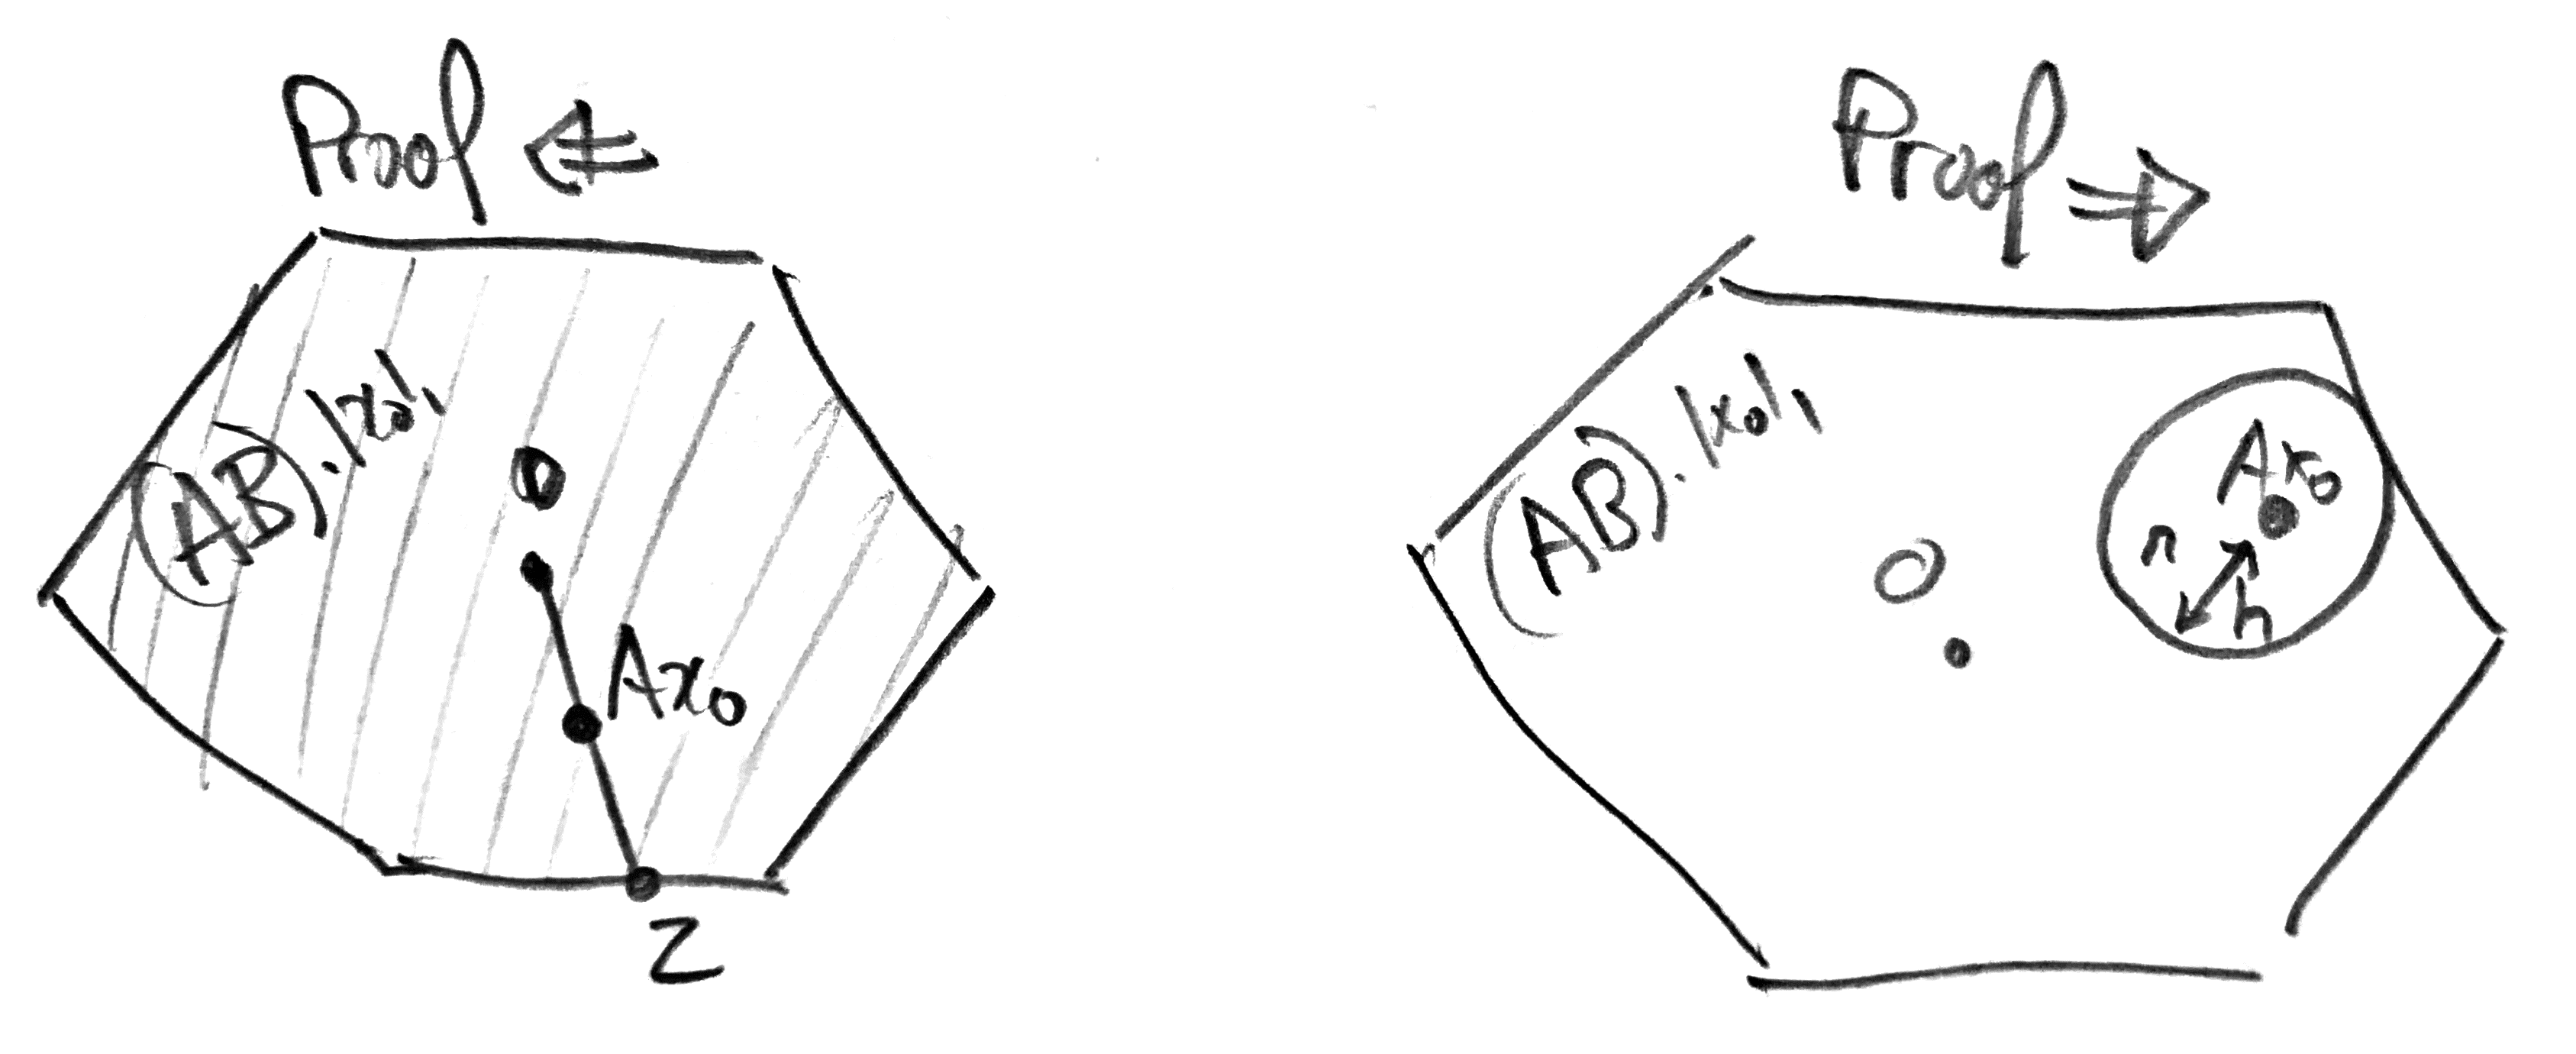
\includegraphics[width=.6\linewidth]{sparse-theory/proofs/polytope-proof-1}
%%
\caption{\label{fig-polytope-proof}
Graphical display of the proof for the polytope analysis of $\ell^1$ exact recovery.
}
\end{figure}

	We now prove ``$\Leftarrow$''. We suppose that $A \frac{x_0}{\norm{x_0}_1} \in \text{int}(AB)$. Then there exists $z$ such that $Ax_0=(1-\de) Az$ and $\norm{z}_1 < \norm{x_0}_1$. This implies $\norm{(1-\de)z}_1 < \norm{x_0}_1$ so that $(1-\de)z$ is better than $x_0$ which is thus not a solution. 
\end{proof}

This results state that ``friendly'' identifiable vectors (those recovered by $\ell^1$) are those who gets projected by $A$ on the boundary of the polytope $\norm{x_0}_1 A B$. Intuitively, if $P$ is small in comparison to $N$, then this projected polytope is small, and most vector will failed to be reconstructed by solving $\ell^1$ minimization. This also suggests why using random projections as in Chapter~\ref{chap-cs}, because somehow they results in a low distortion embedding of the $\ell^1$ ball from $\RR^N$ to $\RR^P$.

Note that if $x_0$ is identifiable, so is $\la x_0$ for $\rho x_0$ for $\rho>0$, and in fact, since the recovery condition only depends on the geometry of the faces of $B$, the obtained condition~\eqref{eq-polytop-ident} only depends on $\sign(x_0)$. 
%
We denote $\Aa : y \mapsto x^\star$ the map from $y$ to a solution of~\eqref{eq-lasso-constr}, which we assume is unique for simplicity of exposition.
%
Condition~\eqref{eq-polytop-ident} thus shows that $A$ and $\Aa$ are inverse bijection on a family of cones $\Cc_s = \enscond{x}{\sign(x)=s}$ and $A\Cc_s$ for certain ``friendly'' sign patterns $s$. These cones $A\Cc_s$ form a partition of the image space $\RR^P$. Assuming for simplicity that the columns $(a_j)_j$ of $A$ have unit norm, for $P=3$, the interaction of these $A\Cc_s$ with the unit sphere of $\RR^3$ for a so-called Delaunay triangulation of the sphere (this construction extends to higher dimension by replacing triangle by simplexes), see also Figure~\ref{fig-delaunay}. Such Delaunay triangulation is characterized by the empty spherical cap property (each circumcircle associated to a triangle should not contains any columns vector $a_j$ of the matrix).
%
Figure~\ref{fig-polytopes} illustrate these conclusions in $\RR^2$ and $\RR^3$. 


\begin{figure}
\centering
%%
\begin{tabular}{@{}c@{}c@{\hspace{3mm}}c@{}}
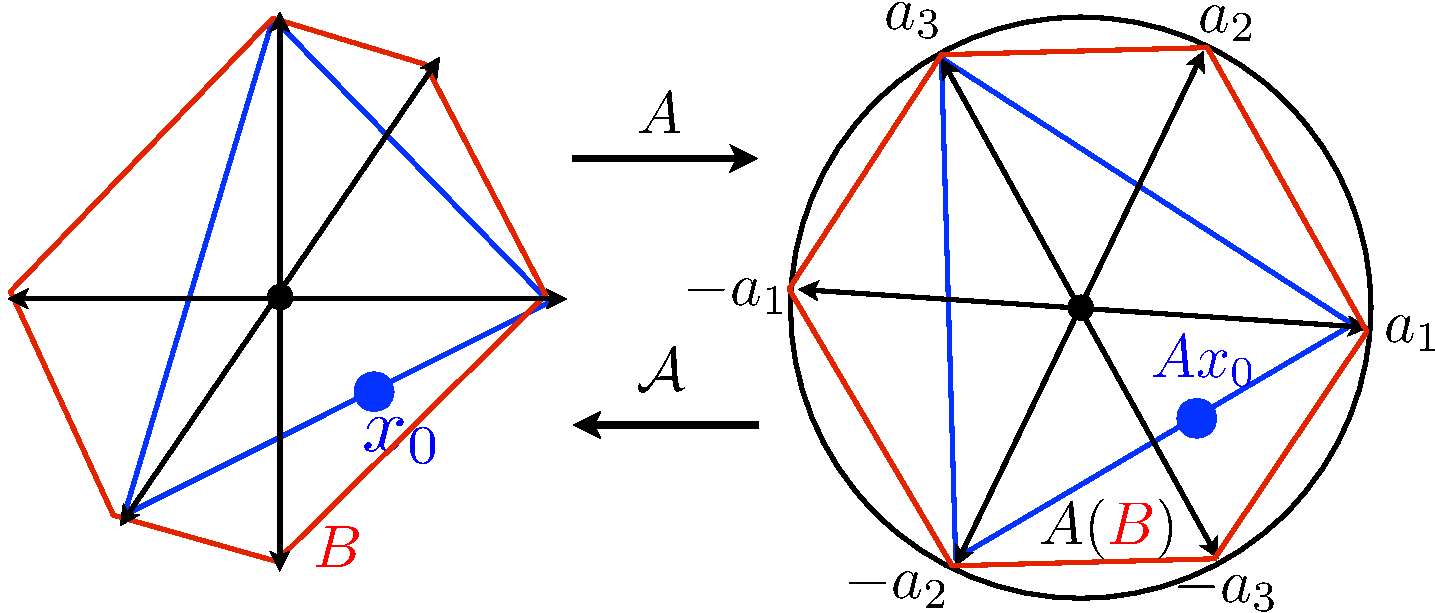
\includegraphics[width=.35\linewidth]{sparse-theory/polytopes/polytopes-32-1}&
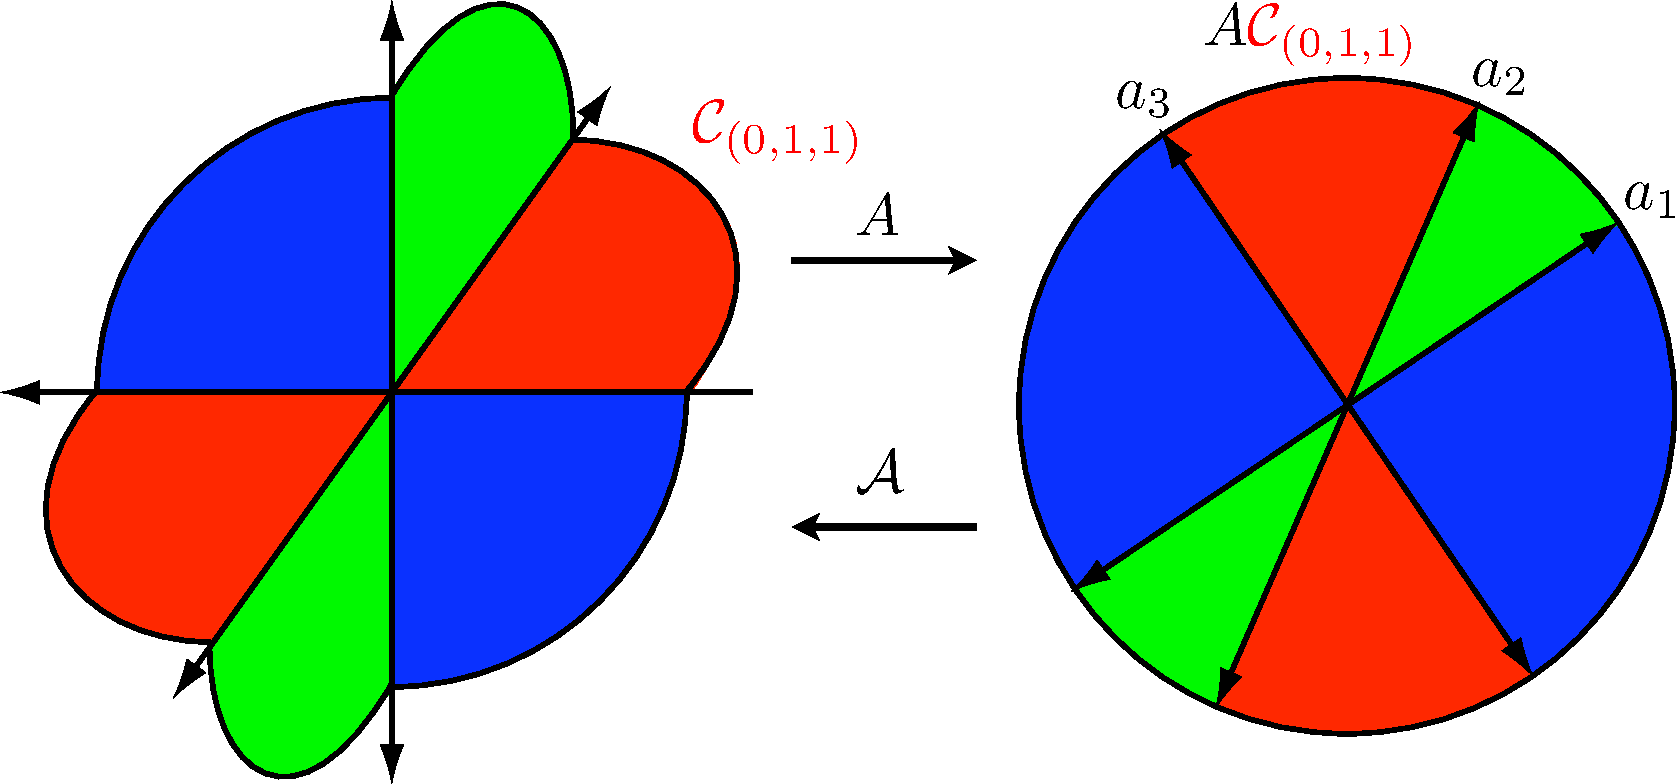
\includegraphics[width=.35\linewidth]{sparse-theory/polytopes/polytopes-32-2}&
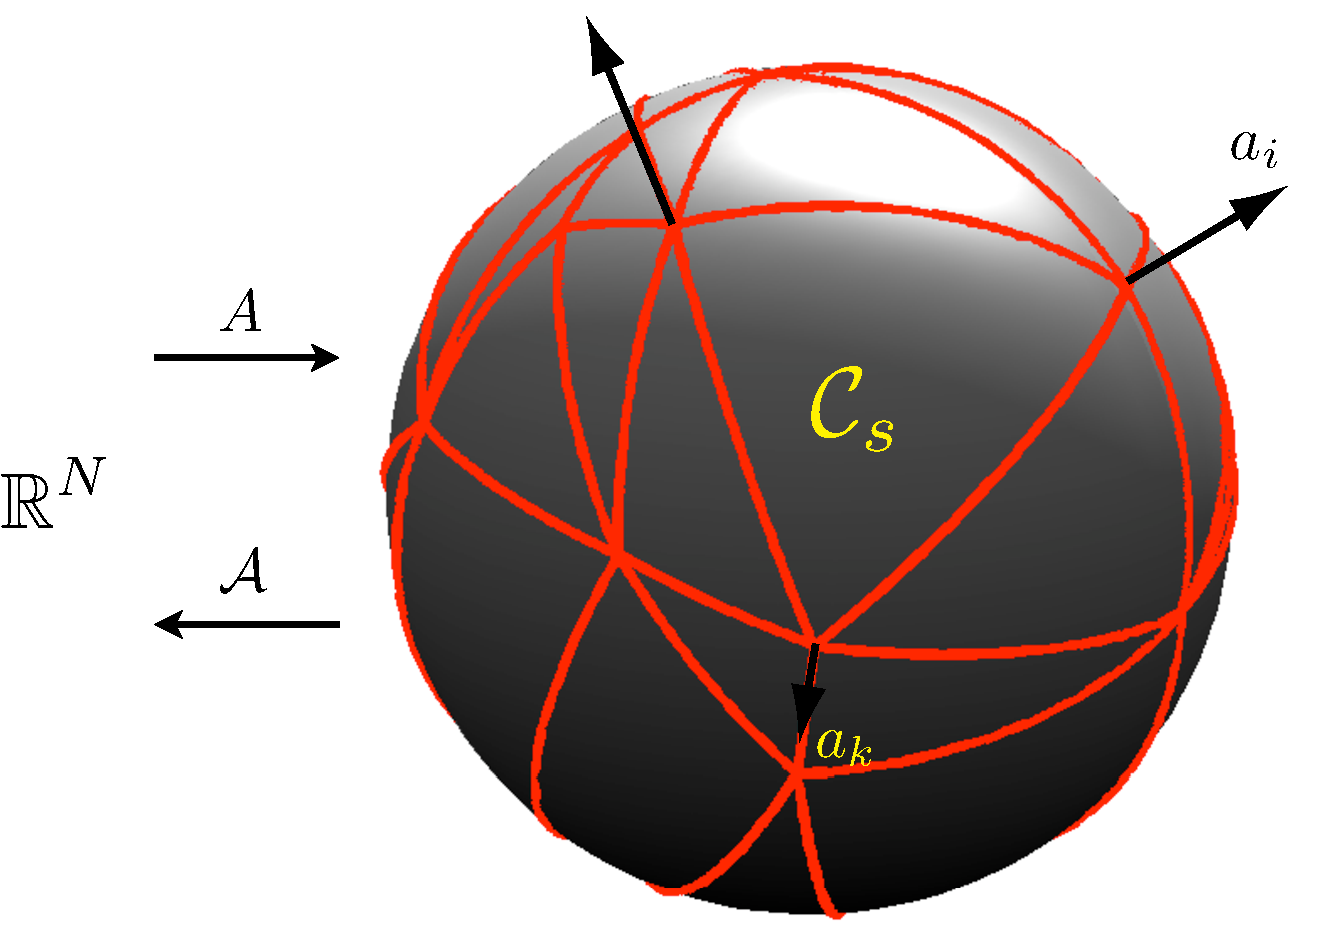
\includegraphics[width=.25\linewidth]{sparse-theory/polytopes/polytopes-3d}\\
$A\in \RR^{2\times 3}$& $A\in \RR^{2\times 3}$ & $A\in \RR^{3\times N}$
\end{tabular}
%%
\caption{\label{fig-polytopes}
Display of the action of the linear map $A$ on the $\ell^1$ ball $B$, and of the inverse non-linear map $\Aa$ defined by the solution of~\eqref{eq-lasso-constr}. 
}
\end{figure}

%%%%%%%%%%%%%%%%%%%%%%%%%%%%%%%%%%%%%%%%%%%%%%%%%%%%%%%%%%%%%%%%%%%%%%%%%%%%%%%%%%
\subsection{Optimality Conditions}

In the following, given an index set $I \subset \{1,\ldots,N\}$, denoting $A=(a_i)_{i=1}^N$ the columns of $A$, we denote $A_I \eqdef (a_i)_{i \in I} \in \RR^{P \times |I|}$ the extracted sub-matrix.  Similarly, for $x \in \RR^N$, we denote $x_I \eqdef (x_i)_{i \in I} \in \RR^{|I|}$. 

The following proposition rephrases the first order optimality conditions in a handy way. 

\begin{prop}\label{prop-first-order-lagr}
	$x_\la$ is a solution to~\eqref{eq-lasso-lagr} for $\la>0$ if and only if
	\eq{
		\eta_{\la,I} = \sign(x_{\la,I})
		\qandq
		\norm{\eta_{\la,I^c}} \leq \la
	}
	where we define
	\eql{\label{eq-defn-eta-lamb}
		I\eqdef \supp(x_\la) \eqdef \enscond{i}{ x_{\la,i} \neq 0 }, 
		\qandq	\eta_\la \eqdef \frac{1}{\la}A^*(y-Ax_\la).
	}
\end{prop}
\begin{proof}
Since~\eqref{eq-lasso-lagr} involves a sum of a smooth and a continuous function, its sub-differential reads
\eq{
	\partial f_\la(x) = \frac{1}{\la}A^*(Ax-y) + \la\partial\norm{\cdot}_1(x).
} 
Thus $x_\la$ is solution to~\eqref{eq-lasso-lagr} if and only if $0 \in \partial f_\la(x_\la)$, which gives the desired result. 
\end{proof}

Note that one has in particular that $\supp(x_\la) \subset \sat(\eta_\la)$.

The following proposition studies the limit case $\la=0$ and introduces the crucial concept of ``dual certificates'', which are the Lagrange multipliers of the constraint $\Ll_y$.

\begin{prop}\label{prop-first-order-constr}
	$x^\star$ being a solution to~\eqref{eq-lasso-constr} is equivalent to having $Ax^\star=y$ and that
	\eql{\label{eq-defn-dual-certif}
		\exists \eta \in \Dd_0(y,x^\star) \eqdef \Im(A^*) \cap \partial \norm{\cdot}_1(x^\star).
	}
\end{prop}
\begin{proof}
Since~\eqref{eq-lasso-constr} involves a sum with a continuous function, one can also computes it sub-differential as
\eq{
	\partial f_0(x) = \partial \iota_{\Ll_y}(x) + \partial\norm{\cdot}_1(x).
}
If $x \in \Ll_y$, then $\partial \iota_{\Ll_y}(x)$ is the linear space orthogonal to $\Ll_y$, i.e. $\ker(A)^\bot=\Im(A^*)$. 
\end{proof}

Note that one has in particular that $\supp(x^\star) \subset \sat(\eta)$ for any valid vector $\eta\in \Dd_0(y,x^\star)$.

Writing $I=\supp(x^\star)$, one thus has
\eq{
	\Dd_0(y,x^\star) = \enscond{ \eta = A^* p }{
		\eta_I = \sign(x^\star_I), \:
		\norm{\eta}_\infty \leq 1
	}.
}
Although it looks like the definition of $\Dd_0(y,x^\star)$ depends on the choice of a solution $x^\star$, convex duality (studied in the next chapter) shows that it is not the case (it is the same set for all solutions).

%%%%%%%%%%%%%%%%%%%%%%%%%%%%%%%%%%%%%%%%%%%%%%%%%%%%%%%%%%%%%%%%%%%%%%%%%%%%%%%%%%
\subsection{Uniqueness}

The following proposition shows that the Lasso selects a set of linearly independent regressors (columns of $A$). This is why this method is also often called ``basis pursuit''. 

\begin{prop}
	For $\la \geq 0$, there is always a solution $x^\star$ to~\eqref{eq-lasso-lagr} with $I=\supp(x^\star)$ such that $\ker(A_I)=\{0\}$
\end{prop}

\begin{proof}
	Let $x$ be a solution and denote $I=\supp(x)$.
	%	
	If $\ker(A_I) \neq \{0\}$, one selects $h_I \in \ker(A_I)$ and define for $t \in \RR$ the vector $x_t \eqdef x+th$.
	We denote $t_0$ the smallest $|t|$ such that $\sign(x_t) \neq \sign(x)$, i.e. $\supp(x_t)$ is strictly included in $I$.
	%
	For $t<t_0$, since $Ax_t=Ax$ and $\sign(x_t)=\sign(x)$, $x_t$ still satisfies the same first order condition as $x_0$, and one can apply  either Proposition~\ref{prop-first-order-constr} (for $\la=0$) or Proposition~\ref{prop-first-order-lagr} (for $\la>0$), so that $x_t$ is a solution of~\eqref{eq-lasso-lagr}.
	%
	Since the minimized function are lower semi continuous, $x_t \rightarrow x_{t_0}$ is still a solution.
	%
	If $\ker(A_{J}) \neq \{0\}$ with $J=\supp(x_{t_0})$, one is over, otherwise one can iterate this argument on $x_{t_0}$ in place of $x$ and have a  sequence of supports which is strictly decaying in size, so it must terminate. 
\end{proof}

\wrapf{sparse-theory/proofs/injectivity}{Trajectory $(x_t)_t$.}
%
This results in particular that if columns of $A_I$ are not independent, then the solution of~\eqref{eq-lasso-lagr} is necessarily non-unique. 

Assuming that $x_\la$ is a solution such that $\ker(A_I)=\{0\}$, then from~\eqref{eq-lasso-lagr},  one obtains the following implicit expression for the solution
\eql{\label{eq-local-shape-lasso}
	x_{\la,I} = A_I^+ y - \la (A_I^*A_I)^{-1} \sign(x_{\la,I}).
}
This expression can be understood as a form of generalized soft thresholding (one retrieve the soft thresholding when $A=\Id_N$). 

The following useful lemma shows that while solutions $x_\la$ to~\eqref{eq-lasso-lagr} are not necessarily unique, the associated ``predictor'' (i.e. denoised version of $y$) $Ax_\la$ is however always uniquely defined.    
%
Note that according to~\eqref{eq-local-shape-lasso}, one has 
\eql{\label{eq-local-shape-lasso}
	\Phi x_{\la} = \Proj_{\Im(A_I)} y - \la A_I (A_I^*A_I)^{-1} \sign(x_{\la,I}).
}
so up to a $O(\la)$ bias, this predictor is an orthogonal projection on a low dimensional subspace indexed by $I$. 


\begin{lem}\label{lem-unique-predict}
	For $\la \geq 0$, if $(x_1,x_2)$ are solution to~\eqref{eq-lasso-lagr}, then $Ax_1=Ax_2$. 
\end{lem}
\begin{proof}
	For $\la=0$, this is trivial because $Ax_1=Ax_2=y$. Otherwise, let us assume $Ax_1 \neq Ax_2$. Then for $x=(x_1+x_2)/2$, one has
	\eq{
		\norm{x}_1 \leq \frac{ \norm{x_1}_1 + \norm{x_2}_2 }{2}
		\qandq
		\norm{Ax-y}^2 < \frac{ \norm{Ax_1-y}^2 + \norm{Ax_2-y}^2 }{2}		
	}
	where the second inequality follows from the strict convexity of the square. This shows that
	\eq{
		\frac{1}{2\la}\norm{Ax-y}^2 +\norm{x}_1 <
		\frac{1}{2\la}\norm{Ax_1-y}^2 +\norm{x_1}_1, 
	}
	which is a contradiction to the optimality of $x_1$. 
\end{proof}


\begin{prop}\label{sec-prop-uniquness-lagr}
 	For $\la>0$, let $x_\la$ be a solution to~\eqref{eq-lasso-lagr} and denote $\eta_\la \eqdef \frac{1}{\la}A^*(y-A x_\la)$.
	%
	We define the ``extended support'' as 
	\eq{
		J \eqdef \sat(\eta_\la) \eqdef \enscond{i}{|\eta_{\la,i}|=1}.
	}
	If $\ker(A_{J})=\{0\}$ then $x_\la$ is the unique solution of~\eqref{eq-lasso-lagr}.
\end{prop}
\begin{proof}
	If $\tilde x_\la$ is also a minimizer, then by Lemma~\ref{lem-unique-predict}, 
	$Ax_\la=A\tilde x_\la$, so that in particular they share the same dual certificate
	\eq{
		\eta_\la = \frac{1}{\la}A^*(y-Ax_\la) = \frac{1}{\la}A^*(y-A\tilde x_\la).
	}
	The first order condition, Proposition~\ref{prop-first-order-lagr}, shows that necessarily 
	$\supp(x_\la) \subset J$ and $\supp(\tilde x_\la) \subset J$.
	%
	Since $A_J x_{\la,J} = A_J \tilde x_{\la,J}$, and since $\ker(A_J)=\{0\}$, one has 
	$x_{\la,J}=\tilde x_{\la,J}$, and thus $x_\la=\tilde x_\la$ because of their supports are included in $J$.
\end{proof}

\begin{prop}\label{sec-prop-uniquness-constr}
 	Let $x^\star$ be a solution to~\eqref{eq-lasso-constr}. If there exists $\eta \in \Dd_0(y,x^\star)$ such that 
	$\ker(A_{J})=\{0\}$ where $J \eqdef \sat(\eta)$ then $x^\star$ is the unique solution of~\eqref{eq-lasso-constr}.
\end{prop}
\begin{proof}
	The proof is the same as for Proposition~\ref{sec-prop-uniquness-lagr}, replacing $\eta_\la$ by $\eta$. 
\end{proof}

These propositions can be used to show that if $A$ is drawn according to a distribution having a density over $\RR^{p \times n}$, then with probability $1$ on the matrix $A$, the solution to~\eqref{eq-lasso-lagr} is unique. Note that this results is not true if $A$ is non random but $y$ is.



%%%%%%%%%%%%%%%%%%%%%%%%%%%%%%%%%%%%%%%%%%%%%%%%%%%%%%%%%%%%%%%%%%%%%%%%%%%%%%%%%%
\subsection{Duality}
\label{sec-duality-lasso}

We now related the first order conditions and ``dual certificate'' introduced above to the duality theory detailed in Section~\ref{sec-cvx-duality}. This is not strictly needed to derive the theory of sparse regularization, but this offers an alternative point of view and allows to better grasp the role played by the certificates. 


\begin{thm}
	For any $\la \geq 0$ (i.e. including $\la=0$), one has strong duality between~\eqref{eq-lasso-lagr} and
	\eql{\label{eq-dual-lasso}
		�\usup{p \in \RR^P} \enscond{ \dotp{y}{p} - \frac{\la}{2} \norm{p}^2 }{ \norm{A^* p}_\infty \leq 1 }.
	}
	One has for any $\la \geq 0$ that $(x^\star,p^\star)$ are primal and dual solutions if and only if
	\eql{\label{eq-pd-support-localization}
		A^* p^\star \in \partial \norm{\cdot}_1(x^\star)
		\quad\Leftrightarrow\quad
		\pa{
		I \subset \sat(A^* p)
		\qandq
		\sign(x_I^\star) = A_I^* p
		}, 
	}
	where we denoted $I=\supp(x^\star)$, 
	%
	and furthermore, for $\la>0$, 
	\eq{
		p^\star = \frac{y-A x^\star}{\la}.
	}
	while for $\la=0$, $Ax^\star=y$.
\end{thm}

\begin{proof}
	There are several ways to derive the same dual. One can for instance directly use the Fenchel-Rockafeller formula~\eqref{eq-fenchel-rockafeller}. But it is instructive to do the computations using Lagrange duality. One can first consider the following re-writing of the primal problem
	\eq{
		\umin{x \in \RR^N} \enscond{ f(z) + \norm{x}_1 }{ Ax=z } = \umin{x \in \RR^N} \usup{p \in \RR^p} \Ll(x,z,p) \eqdef f_\la(z) + \norm{x}_1 + \dotp{z-Ax}{p}
	}
	where $f_\la(z) \eqdef \frac{1}{2\la}\norm{z-y}^2$ if $\la>0$ and $f(z)=\iota_{\{y\}}(z)$ if $\la=0$.
	%
	For $\la>0$ since $f_\la$ and $\norm{\cdot}_1$ are continuous, strong duality holds. 
	%
	For $\la=0$, since the constraint appearing in $f_0$ is linear (actually a singleton), strong duality holds also. 
	%
	Thus using Theorem~\ref{thm-strong-duality}, one can exchange the min and the max and obtains
	\eq{
		\umax{p \in \RR^P}�\pa{�\min{z}�\dotp{z}{p}+ f_\la(z)  } +�\pa{ \min{x}�\norm{x}_1 - \dotp{x}{A^*p} }
		= \umax{p \in \RR^P} - f_\la^*( -p ) - (\norm{\cdot}_1)^*( A^* p ).
	}
	Using~\eqref{prop-dual-lp}, one has that $(\norm{\cdot}_1^* = \iota_{\norm{\cdot}_\infty \leq 1}$. 
	%
	For $\la>0$, one has using Proposition~\ref{eq-example-legendre} that 
	\eq{
		f_\la^* = ( \frac{1}{2\la}\norm{\cdot-y}^2 )^* = \frac{1}{\la} ( \frac{1}{2}\norm{\cdot-y}^2 )^*(\la \cdot)
		=   \frac{1}{2\la} \norm{\la \cdot}^2 + \dotp{\cdot}{y}
	}
	which gives the desired dual problem. 
	%
	The first order optimality conditions read $Ax^\star=z^\star$ and
	\eq{
		0 \in \partial \norm{\cdot}_1(x^\star) - A^* p^\star
		\qandq
		0 \in \partial f_\la(z^\star) + p^\star.
	}
	The first condition is equivalent to~\eqref{eq-pd-support-localization}.
	For $\la>0$, $f_\la$ is smooth, and the second condition is equivalent to 
	\eq{
		p^\star = \frac{y-A^* x^\star}{\la}
		\qandq
		A^* p^\star \in \partial \norm{\cdot}_1(x^\star)
	}
	which are the desired formula.
	%
	For $\la=0$, the second condition holds as soon as $z^\star = Ax^\star=y$.
\end{proof}


Note that in the case $\la>0$,~\eqref{eq-dual-lasso} is strongly convex, and in fact the optimal solution $p_\la$ is computed as an orthogonal projection
\eq{
	p_\la \in \uargmin{p \in \RR^P} \enscond{ \norm{p-y/\la} }{ \norm{A^* p}_\infty \leq 1 }. 
}
The sup in~\eqref{eq-dual-lasso} is thus actually a max if $\la>0$. If $\la>0$, in case $\ker(A^*)=\Im(A)^\bot=\{0\}$, the constraint set of the dual is bounded, so that the sup is also a max. 


%%%%%%%%%%%%%%%%%%%%%%%%%%%%%%%%%%%%%%%%
%%%%%%%%%%%%%%%%%%%%%%%%%%%%%%%%%%%%%%%%
%%%%%%%%%%%%%%%%%%%%%%%%%%%%%%%%%%%%%%%%
\section{Consistency and Sparsitency}

%%%%%%%%%%%%%%%%%%%%%%%%%%%%%%%%%%%%%%%%
\subsection{Bregman Divergence Rates for General Regularizations}

Here we consider the case of a general regularization of the form 
\eql{\label{eq-lagr-J}
	\umin{x \in \RR^N} \frac{1}{2\la}\norm{Ax-y}^2+J(x)
}
for a convex regularizer $J$.

\begin{figure}
\centering
%%
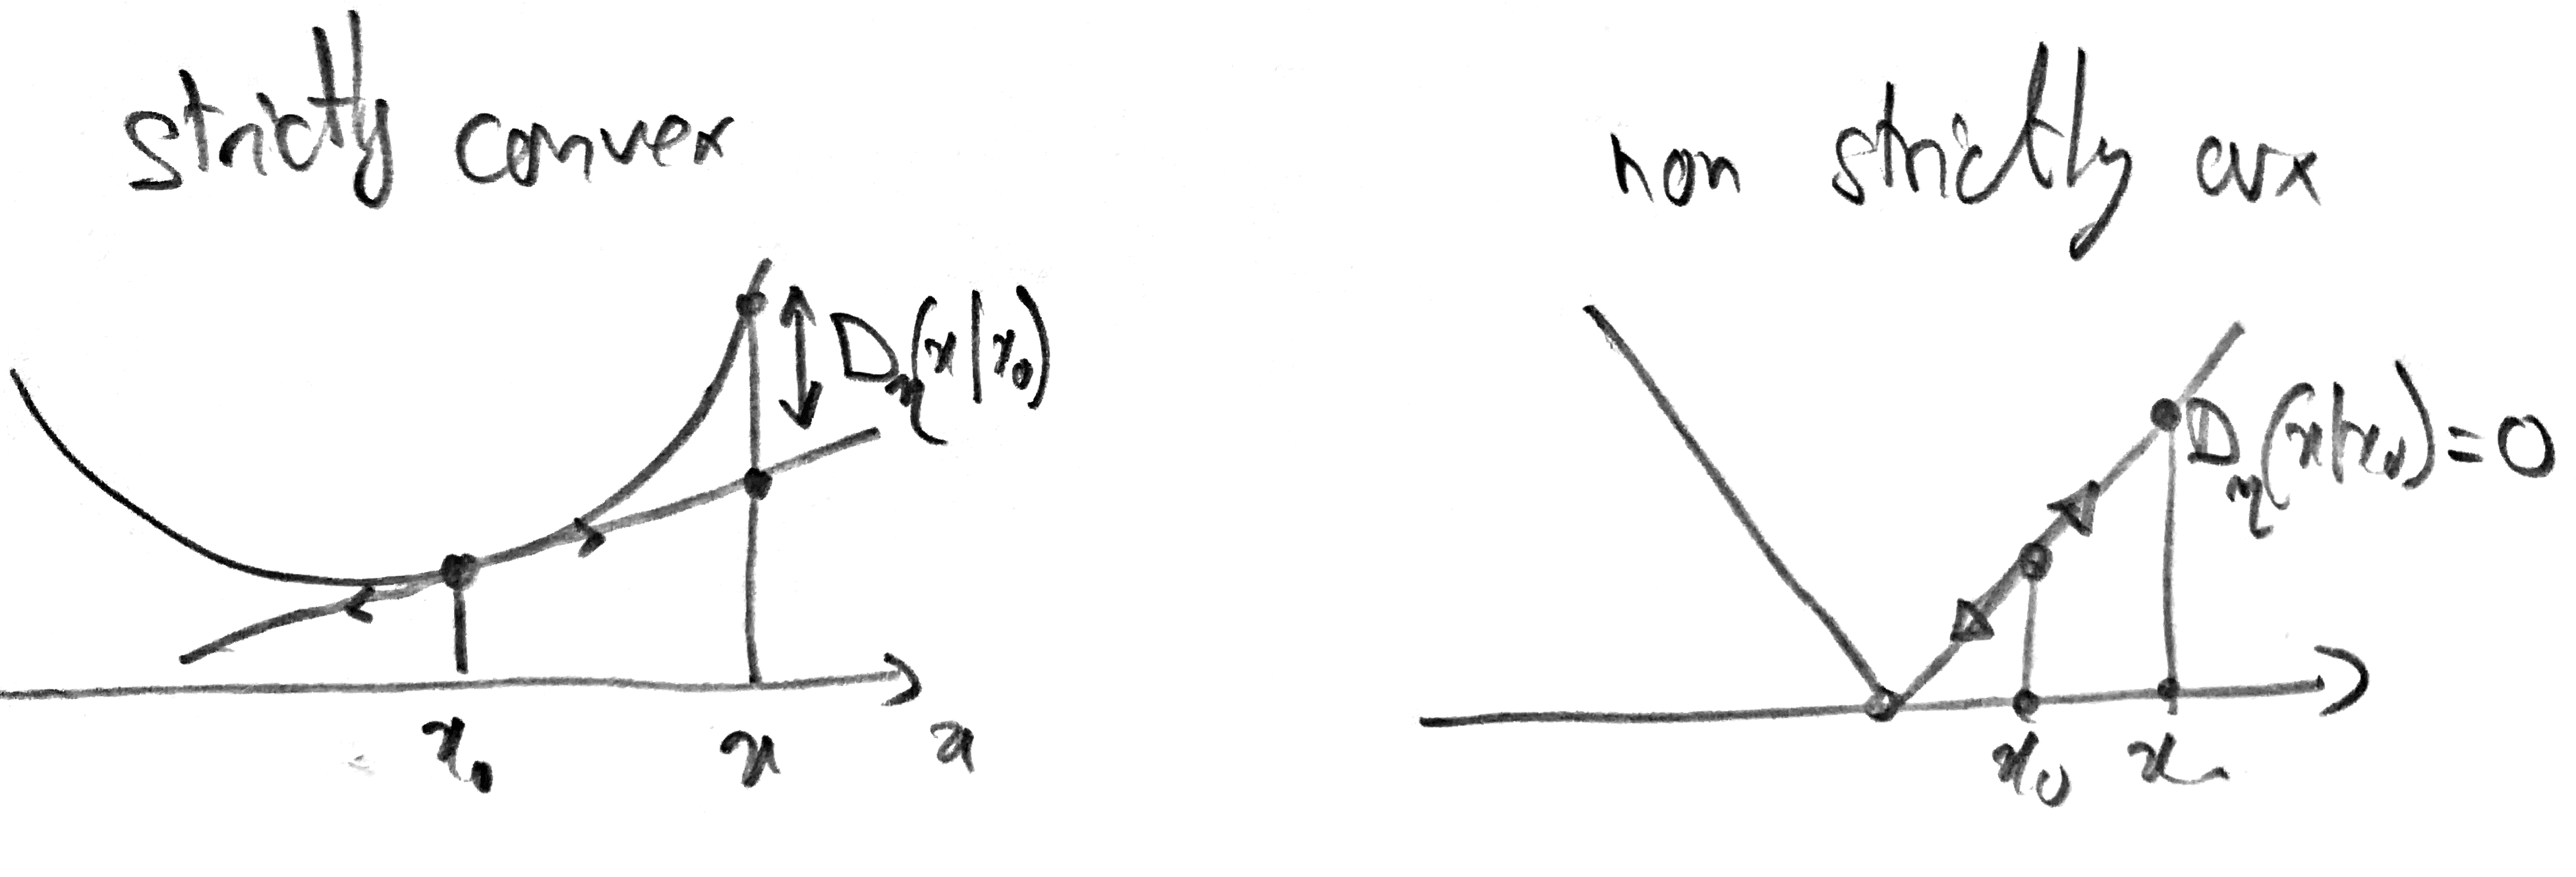
\includegraphics[width=.6\linewidth]{sparse-theory/proofs/bregman}
%%
\caption{\label{fig-bregman}
Visualization of Bregman divergences.
}
\end{figure}

For any $\eta \in \partial J(x_0)$, we define the associated Bregman divergence as
\eq{
	D_\eta(x|x_0) \eqdef J(x)-J(x_0)-\dotp{\eta}{x-x_0}.
}
One has $D_\eta(x_0|x_0)$, and since $J$ is convex, one has $D_\eta(x|x_0) \geq 0$ \todo{put here drawings}.

In the case where $J$ is differentiable, since $\partial J(x_0)=\{\nabla J(x_0)\}$, this divergence simply reads
\eq{
	D(x|x_0) \eqdef J(x)-J(x_0)-\dotp{\nabla J(x_0)}{x-x_0}.
}
If furthermore $J$ is strictly convex, then $D(x|x_0)=0$ if and only if $x=x_0$, so that $D(\cdot|\cdot)$ is similar to a distance function (but it does not necessarily satisfies the triangular inequality.

If $J=\norm{\cdot}^2$, then $D(x|x_0) = \norm{x-x_0}^2$ is the Euclidean norm. 
%
If $J(x) = \sum_i x_i (\log(x_i)-1) + \iota_{\RR^+}(x_i)$ is the entropy, then 
\eq{
	D(x|x_0)  = \sum_i x_i \log\pa{ \frac{x_i}{x_{0,i}} } + x_{0,i}-x_i
}
is the so-called Kulback-Leibler divergence on $\RR_+^N$. 

The following theorem, which is due to Burger-Osher, state a linear rate in term of this Bregman divergence.

\begin{thm}\label{thm-bregman-rates}
	If there exists 
	\eql{\label{eq-sourcecond-J}
		\eta  = A^* p \in \Im(A^*) \cap \partial J(x_0), 
	}
	then one has for any $x_\la$ solution of~\eqref{eq-lagr-J}
	\eql{\label{eq-bregman-rate}
		D_\eta( x_\la|x_0 ) \leq \frac{1}{2}\pa{ \frac{\norm{w}}{\sqrt{\la}} + \sqrt{\la}\norm{p} }^2.
	}
	Futhermore, one has the useful bound
	\eql{\label{eq-predict-source}
		\norm{Ax_\la-y} \leq \norm{w} + (\sqrt{2}+1) \norm{p} \la.
	}
\end{thm}
\begin{proof}
	The optimality of $x_\la$ for~\eqref{eq-lagr-J} implies
	\eq{
		\frac{1}{2\la}\norm{Ax_\la-y}^2+J(x_\la) \leq \frac{1}{2\la}\norm{Ax_0-y}^2+J(x_0) = \frac{1}{2\la}\norm{w}^2+J(x_0).
	}
	Hence, using $\dotp{\eta}{x_\la-x_0} = \dotp{p}{Ax_\la-Ax_0} = \dotp{p}{A x_\la - y+w}$, one has
	\begin{align*}
		D_\eta(x_\la|x_0) &= J(x_\la)-J(x_0)-\dotp{\eta}{x_\la-x_0} 
			\leq \frac{1}{2\la}\norm{w}^2 - \frac{1}{2\la}\norm{Ax_\la-y}^2 -\dotp{p}{A x_\la-y} - \dotp{p}{w} \\
			& = \frac{1}{2\la}\norm{w}^2 - \frac{1}{2\la}\norm{Ax_\la-y + \la p }^2 + \la \norm{p}^2 - \dotp{p}{w} \\
			& \leq \frac{1}{2\la}\norm{w}^2 + \frac{\la}{2} \norm{p}^2 + \norm{p}\norm{w}
			= \frac{1}{2}\pa{ \frac{\norm{w}}{\sqrt{\la}} + \sqrt{\la}\norm{p} }^2.
	\end{align*}
	From the second line above, since $D_\eta(x_\la|x_0) \geq 0$, one has using Cauchy-Schwartz
	\eq{
		\norm{Ax_\la-y + \la p }^2 \leq \norm{w}^2 + 2 \la^2 \norm{p}^2 + 2 \la\norm{p} \norm{w} 
		\leq 
		\norm{w}^2 + 2 \sqrt{2}\norm{p} \norm{w} \la  + 2 \la^2 \norm{p}^2
		= \pa{ \norm{w} + \sqrt{2}\la \norm{p} }^2.
	}
	Hence
	\eq{
		\norm{Ax_\la-y } \leq \norm{Ax_\la-y + \la p } + \la \norm{p}
		\leq \norm{w} + \sqrt{2}\la \norm{p} + \la \norm{p}.
	}
\end{proof}

Choosing $\la = \norm{w}/\norm{p}$ in~\eqref{eq-bregman-rate}, one thus obtain a linear rate in term of Bregman divergence $D_\eta( x_\la|x_0 ) \leq 2 \norm{w}\norm{p}$. 
%
For the simple case of a quadratic regularized $J(x)=\norm{x}^2/2$, as used in Section~\ref{}, one sees that the source conditions~\eqref{eq-sourcecond-J} simply reads
\eq{
	x_0 \in \Im(A^*)
}
which is equivalent to~\eqref{eq-source-cond-init} with exponent $\be=\frac{1}{2}$, and under this condition,~\eqref{eq-bregman-rate} gives the following sub-linear rate in term of the $\ell^2$ norm
\eq{
	\norm{x_0-x_\la} \leq 2 \sqrt{ \norm{w}\norm{p} }.
}
\todo{This seems inconsistent, this should corresponds to $\be=1$ to obtain the same rates in both theorems!}

%
Note that the ``source condition''~\eqref{eq-sourcecond-J} is equivalent to $x_0$ such that $Ax_0=y$ is a solution to the constraint problem
\eq{
	\umin{Ax=y} J(x). 
}
So simply being a solution of the constraint noiseless problem thus implies a linear rate for the resolution of the noisy problem in term of the Bregman divergence.




%%%%%%%%%%%%%%%%%%%%%%%%%%%%%%%%%%%%%%%%
\subsection{Linear Rates in Norms for $\ell^1$ Regularization}

The issue with the control~\eqref{eq-bregman-rate} of the error in term of Bregman divergence is that it is not ``distance-like'' for regularizers $J$ which are not strictly convex. This is in particular the case for the $\ell^1$ norm $J=\norm{\cdot}_1$ which we now study. 

	\wrapf{sparse-theory/proofs/bregman-l1}{Controlling Bregman divergence with the $\ell^1$ norm when $\eta$ is not saturating.}
	
The following fundamental lemma shows however that this Bregman divergence for $\ell^1$ behave like a distance (and in fact controls the $\ell^1$ norm) on the indexes where $\eta$ does not saturate. 

\begin{lem}
	For $\eta \in \partial \norm{\cdot}_1(x_0)$, let $J \eqdef \sat(\eta)$. Then
	\eql{\label{eq-bound-breg-source}
		D_\eta(x|x_0) \geq (1-\norm{\eta_{J^c}}_\infty) \norm{(x-x_0)_{J^c}}_1.
	}
\end{lem}

\begin{proof}
Note that $x_{0,J^c}=0$ since $\supp(x_0) \subset \sat(\eta)$ by definition of the sub-differential of the $\ell^1$ norm. 
%
	Since the $\ell^1$ norm is separable, each term in the sum defining $D_\eta(x|x_0)$ is positive, hence
	\begin{align*}
		D_\eta(x|x_0) &= \sum_i |x_i|-|x_{0,i}|- \eta_i ( x_{i}-x_{0,i} ) 
			\geq \sum_{i \in J^c} |x|-|x_0|- \eta_i ( x_{i}-x_{0,i} ) \\
		&= \sum_{i \in J^c} |x_i|- \eta_i x_{i} \geq \sum_{i \in J^c} (1-|\eta_i|) |x_i|
		\geq (1-\norm{\eta_{J^c}}_\infty) \sum_{i \in J^c} |x_i|
		= (1-\norm{\eta_{J^c}}_\infty) \sum_{i \in J^c} |x_i-x_{0,i}|.
	\end{align*}
\end{proof}

The quantity $1-\norm{\eta_{J^c}}_\infty>0$ controls how much $\eta$ is ``inside'' the sub-differential. The larger this coefficients, the better is the control of the Bregman divergence.  

The following theorem uses this lemma to state the convergence rate of the sparse regularized solution, under the same hypothesis has Proposition~\ref{sec-prop-uniquness-constr} (with $x^\star=x_0$).

\begin{thm}\label{thm-linrate-l1}
	If there exists 
	\eql{\label{eq-sourcecond-l1}
		\eta \in \Dd_0(A x_0,x_0)
	}
	and $\ker(A_{J})=\{0\}$ where
	$J \eqdef \sat(\eta)$ then choosing $\la = c \norm{w}$, there exists $C$ (depending on $c$) such that any solution $x_\la$ of $\Pp(A x_0+w)$ satisfies
	\eql{\label{eq-linrate-l1}
		\norm{x_\la-x_0} \leq C \norm{w}. 
	}
\end{thm}
\begin{proof}
	We denote $y=A x_0+w$.
	%
	The optimality of $x_\la$ in~\eqref{eq-lasso-lagr} implies
	\eq{
		\frac{1}{2\la} \norm{Ax_\la-y}^2 + \norm{x_\la}_1 \leq 
		\frac{1}{2\la} \norm{Ax_0-y}^2 + \norm{x_0}_1 = \frac{1}{2\la} \norm{w}^2 + \norm{x_0}_1
	}
	and hence
	\eq{
		\norm{Ax_\la-y}^2 \leq \norm{w}^2 + 2\la \norm{x_0}_1
	}
	%
	Using the fact that $A_J$ is injective, one has $A_J^+A_J=\Id_{J}$, so that
	\begin{align*}
		\norm{(x_\la-x_0)_J}_1 &= \norm{A_J^+ A_J(x_\la-x_0)_J}_1
			\leq \norm{A_J^+}_{1,2} \norm{ A_J x_{\la,J} - y + w }
			\leq \norm{A_J^+}_{1,2} \pa{ \norm{ A_J x_{\la,J} - y } + \norm{w} }  \\
			& \leq 
			\norm{A_J^+}_{1,2} \pa{ \norm{ A x_{\la} - y } + \norm{A_{J^c} x_{\la,J^c}} + \norm{w} }\\
			&\leq 
			\norm{A_J^+}_{1,2} \pa{ \norm{ A x_{\la} - y } + \norm{A_{J^c}}_{2,1} \norm{ x_{\la,J^c} - x_{0,J^c} }_1 + \norm{w} } \\
			&\leq 
			\norm{A_J^+}_{1,2} \pa{ \norm{w} + (\sqrt{2}+1) \norm{p} \la + \norm{A_{J^c}}_{2,1} \norm{ x_{\la,J^c} - x_{0,J^c} }_1 + \norm{w} } 			
	\end{align*}
	where we used $x_{0,J^c}=0$ and~\eqref{eq-predict-source}. 
	One plug this bound in the decomposition, and using~\eqref{eq-bound-breg-source} and~\eqref{eq-bregman-rate}
	\begin{align*}
		\norm{x_\la-x_0}_1 &= \norm{(x_\la-x_0)_J}_1 + \norm{(x_\la-x_0)_{J^c}}_1 \\
		& \leq \norm{(x_\la-x_0)_{J^c}}_1 \pa{ 1 + \norm{A_J^+}_{1,2} \norm{A_{J^c}}_{2,1} }
		+ \norm{A_J^+}_{1,2} \pa{   (\sqrt{2}+1) \norm{p} \la + 2 \norm{w}�}		\\
		& \leq \frac{D_\eta(x|x_0)}{1-\norm{\eta_{J^c}}_\infty} \pa{ 1 + \norm{A_J^+}_{1,2} \norm{A_{J^c}}_{2,1} }
		+ \norm{A_J^+}_{1,2} \pa{   (\sqrt{2}+1) \norm{p} \la + 2 \norm{w}�} \\
		& \leq \frac{ 
				\frac{1}{2}\pa{ \frac{\norm{w}}{\sqrt{\la}} + \sqrt{\la}\norm{p} }^2
			}{1-\norm{\eta_{J^c}}_\infty} \pa{ 1 + \norm{A_J^+}_{1,2} \norm{A_{J^c}}_{2,1} }
		+ \norm{A_J^+}_{1,2} \pa{   (\sqrt{2}+1) \norm{p} \la + 2 \norm{w}�}. 
	\end{align*}	
	Thus setting $\la=c\norm{w}$, one obtains the constant
	\eq{
		C \eqdef \frac{ 
				\frac{1}{2}\pa{ \frac{1}{\sqrt{c}} + \sqrt{c}\norm{p} }^2
			}{1-\norm{\eta_{J^c}}_\infty} \pa{ 1 + \norm{A_J^+}_{1,2} \norm{A_{J^c}}_{2,1} }
		+ \norm{A_J^+}_{1,2} \pa{   (\sqrt{2}+1) \norm{p} c + 2 �}.
	}
\end{proof}


Note that this theorem does not imply that $x_\la$ is a unique solution, only $x_0$ is unique in general.
%
The condition~\eqref{eq-sourcecond-l1} is often called a ``source condition'', and is strengthen by imposing a non-degeneracy $\ker(A_{J})=\{0\}$. This non-degeneracy imply some stability in $\ell^2$ sense~\eqref{eq-linrate-l1}.
%
The result~\eqref{eq-linrate-l1} shows a linear rate, i.e. the (possibly multi-valued) inverse map $y \mapsto x_\la$ is Lipschitz continuous.


It should be compared with Theorem~\ref{thm-sublin-quad} on linear methods for inverse problem regularization, which only gives sub-linear rate.
%
The sources conditions in the linear~\eqref{eq-source-cond-init} and non-linear~\eqref{eq-sourcecond-l1} cases are however very different.
%
In the linear case, for $\be=1/2$, it reads $x_0 \in \Im(A^*)=\ker(A)^\bot$, which is mandatory because linear method cannot recover anything in $\ker(A)$.
%
On contrary, the non-linear source condition only requires that $\eta$ to be in $\Im(A^*)$, and is able (in the favorable cases of course) to recover information in $\ker(A)$. 

 
 
%%%%%%%%%%%%%%%%%%%%%%%%%%%%%%%%%%%%%%%%
\subsection{Sparsistency}
\label{sec-sparsistency}

Theorem~\ref{thm-linrate-l1} is abstract in the sense that it rely on hypotheses which are hard to check.
%
The crux of the problem, to be able to apply this theorem, is to be able to ``construct'' a valid certificate~\eqref{eq-sourcecond-l1}. 
%
We now give a powerful ``recipe'' which -- when it works -- not only give a sufficient condition for linear rate, but also provides ``support stability''.


For any solution $x_\la$ of $(\Pp_\la(y))$, as already done in~\eqref{eq-defn-eta-lamb}, we define the (unique, independent of the chosen solution) dual certificate 
\eq{
	\eta_\la \eqdef A^* p_\la
	\qwhereq
	p_\la \eqdef \frac{y - A x_\la}{\la}.
}
The following proposition shows that $p_\la$ converge to a very specific dual certificate of the constrained problem, which we coined ``minimal norm'' certificate. 

\begin{prop}
	If $y = A x_0$ where $x_0$ is a solution to $(\Pp_\la(y=A x_0))$, one has
	\eql{\label{eq-minnorm-certif}
		p_\la \rightarrow p_0 \eqdef
		\uargmin{p \in \RR^P} \enscond{\norm{p}}{ A^* p \in \Dd_0(y,x_0) }.
	}
	The vector $\eta_0 \eqdef A^* p_0$ is called the ``minimum norm certificate''. 
\end{prop}
\begin{proof}
	This follows from the fact that $p_\la$ is the unique solution to~\eqref{eq-dual-lasso} and then applying the same proof as the one done in Proposition~\ref{prop-gamma-conv-regul}�to study the small $\la$ limit of penalized problems. 
\end{proof}

This proposition shows that, while dual certificate $\Dd_0(y,x_0)$ for $\la=0$ are non-unique, taking the limit as $\la\rightarrow 0$ singles-out a specific one, which is of paramount importance to study stability of the support when the noise and $\la$ are small. 

A major difficulty in computing~\eqref{eq-minnorm-certif} is that it should satisfy the non-linear constraint $\norm{\eta_0}_\infty$. One thus can ``simplify'' this definition by removing this $\ell^\infty$ constraint and define the so-called  ``minimum norm certificate''
\eql{\label{eq-minnorm-certif}
	\eta_F \eqdef A^* p_F
	\qwhereq 
	p_F \eqdef
	\uargmin{p \in \RR^P} \enscond{\norm{p}}{ A_I^* p = \sign(x_{0,I}) }.
}
The notation ``$\eta_F$'' refers to the ``Fuchs'' certificate, which we named in honour of J-J. Fuchs who first used it to study $\ell^1$ minimization. 

We insists that $p_F$ is not necessarily a valid certificate (hence the naming ``pre-certificate'') since one does not have in general $\norm{\eta_F}_\infty \leq 1$. 
%
The vector $p_F$ is a least square solution to the linear system $A_I^* p = \sign(x_{0,I})$, and it can thus be compute in closed form using the pseudo-inverse $p_F=A_I^{*,+} \sign(x_{0,I})$ (see Proposition~\eqref{prop-pseudo-inv}). In case $\ker(A_I)=\{0\}$, one has the simple formula
\eq{
	p_F = A_I (A_I^*A_I)^{-1} \sign(x_{0,I}).
}
Denoting $C \eqdef A^* A$ the ``correlation'' matrix, one has the nice formula 
\eql{\label{eq-eta-f-cov}
	\eta_F = C_{\cdot,I} C_{I,I}^{-1} \sign(x_{0,I}).
}
The following proposition relates $\eta_F$ to $\eta_0$, and shows that $\eta_F$ can be used as a ``proxy'' for $\eta_0$

\begin{prop}
	If $\norm{\eta_F}_\infty \leq 1$, then $p_F=p_0$ and $\eta_F=\eta_0$.
\end{prop}

The condition $\norm{\eta_F}_\infty \leq 1$ implies that $x_0$ is solution to~\eqref{eq-lasso-constr}. 
% 
The following theorem shows that if one strengthen this condition to impose a non-degeneracy on $\eta_F$, then one has linear rate with a stable support in the small noise regime.

Before proceeding to the proof, let us note that the constraint $\norm{\eta_F}_\infty \leq 1$ corresponds to the definition of the spherical Delaunay triangulation, as highlighted by Figure~\ref{fig-delaunay}. This remark was made to us by Charles Dossal.

\begin{figure}
\centering
%%
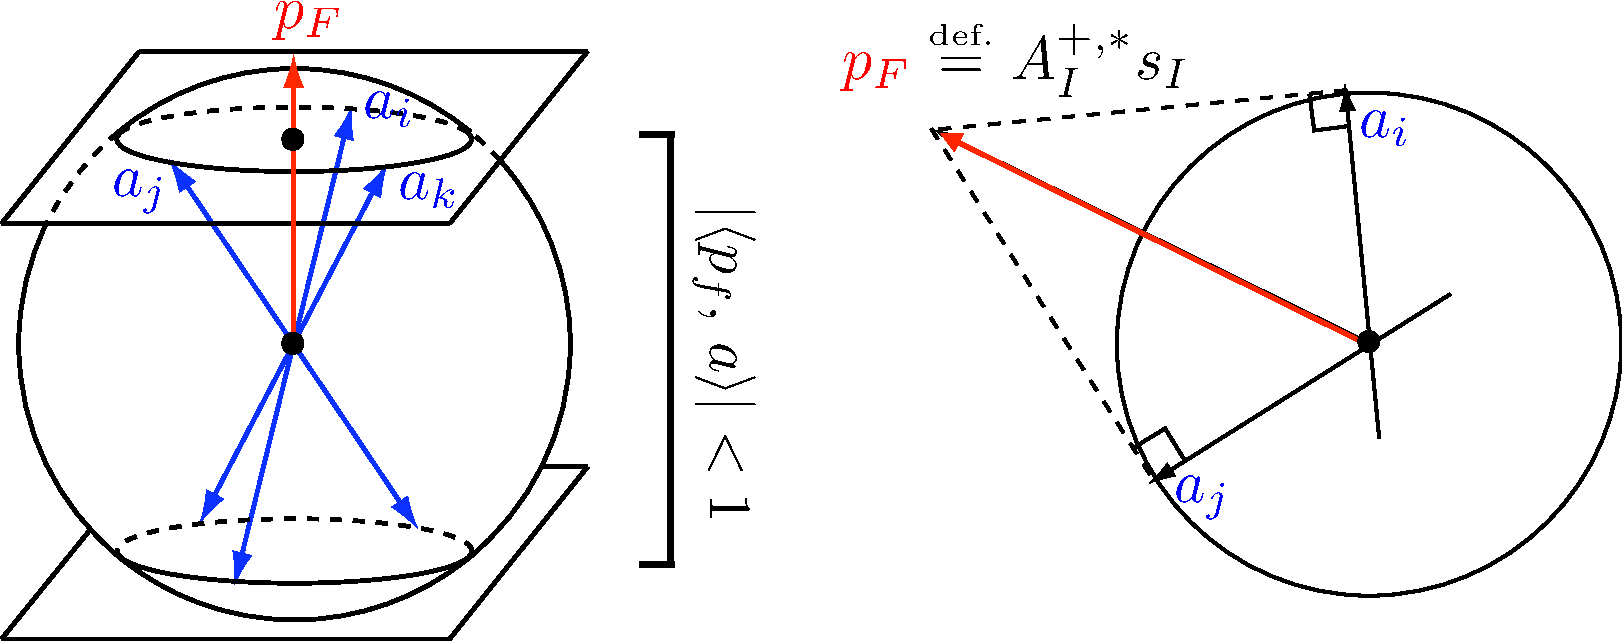
\includegraphics[width=.6\linewidth]{sparse-theory/polytopes/delaunay}
%%
\caption{\label{fig-delaunay}
Visualization of the condition that $\norm{\eta_F}_\infty \leq 1$ as a spherical Delaunay triangulation constraint that all Delaunay spherical caps indexes by identifiable vector should be empty of $(\pm a_i)_i$. 
}
\end{figure}

\begin{rem}[Operator norm]\label{rem-operator-norm}
In the proof, we use the $\ell^p-\ell^q$ matrix operator norm, which is defined as
\eq{
	\norm{B}_{p,q} \eqdef \max \enscond{ \norm{B u}_q }{ \norm{u}_p \leq 1 }.
}
For $p=q$, we denote $\norm{B}_{p} \eqdef \norm{B}_{p,p}$.
%
For $p=2$, $\norm{B}_2$ is the maximum singular value, and one has
\eq{
	\norm{B}_1 = \umax{j} \sum_i |B_{i,j}|
	\qandq
	\norm{B}_\infty = \umax{i} \sum_j |B_{i,j}|.
}
\end{rem}

\begin{thm}\label{thm-support-stable}
	If 
	\eq{
		\norm{\eta_F}_\infty \leq 1
		\qandq 
		\norm{\eta_{F,I^c}}_\infty<1, 
	}
	and $\ker(A_I) = \{0\}$, 
	then there exists $C,C'$ such that if $\max(\norm{w}, \norm{w}/\la) \leq C$, then the solution $x_\la$ of~\eqref{eq-lasso-lagr} is unique, is supported in $I$, and in fact
	\eql{\label{eq-explicit-lownoise}
		x_{\la,I} = x_{0,I} + A_I^+ w - \la (A_I^*A_I)^{-1} \sign(x_{0,I}^\star).
	}
	In particular, $\norm{x_\la-x_0} = O(\norm{A^* w}_\infty) = O(\norm{w})$.
\end{thm}

\begin{proof}
	In the following we denote $T \eqdef \min_{i \in I} |x_{0,i}|$ the signal level, and $\de \eqdef \norm{A^* w}_\infty$
	which is the natural way to measure the noise amplitude in the sparse setting. 
	%
	We define $s \eqdef \sign(x_0)$, and consider the ``ansatz''~\eqref{eq-explicit-lownoise} and thus define the following candidate solution
	\eql{
		\hat x_{I} \eqdef x_{0,I} + A_I^+ w - \la (A_I^*A_I)^{-1} s_I, 
	}
	and $\hat x_{I^c}=0$. The goal is to show that $\hat x$ is indeed the unique solution of~\eqref{eq-lasso-lagr}. 
	
	
	\noindent\textit{Step 1.}  The first step is to show sign consistency, i.e. that $\sign(\hat x)=s$. This is true if $\norm{x_{0,I}-\hat x_I}_\infty < T$, and is thus implied by
	\eql{\label{eq-supp-stab-proof-1}
		\norm{x_{0,I}-\hat x_I}_\infty \leq K \norm{A_I^* w}_\infty + K \la < T
		\qwhereq
		K \eqdef \norm{(A_I^*A_I)^{-1}}_{\infty}, 
	}
	where we used the fact that $A_I^+ = (A_I^*A_I)^{-1} A_I^*$.
	
	\noindent\textit{Step 2.} The second step is to check the first order condition of Proposition~\ref{sec-prop-uniquness-lagr}, i.e. $\norm{\hat \eta_{I^c}}_\infty < 1$, where $\la \hat \eta = A^* (y-A \hat x)$. This implies indeed that $\hat x$ is the unique solution of~\eqref{eq-lasso-lagr}. One has
	\begin{align*}
		\la \hat \eta &= A^* (A_I x_{0,I} + w - A_I \pa{ x_{0,I} + A_I^+ w - \la (A_I^*A_I)^{-1} s_I ) } \\
			&=  A^* ( A_I A_I^+ - \Id ) w + \la \eta_F.
	\end{align*}
	The condition $\norm{\hat \eta_{I^c}}_\infty < 1$ is thus implied by
	\eql{\label{eq-supp-stab-proof-2}		
		\norm{A_{I^c}^* A_I (A_I^*A_I)^{-1}}_\infty \norm{A_I^* w}_\infty + \norm{A_{I^c}^* w}_\infty + \la \norm{\eta_{F,I^c}}_\infty 
		\leq 
		R \norm{A_I^* w}_\infty - S \la <0
	}	
	\eq{
		R \eqdef K L + 1 
		\qandq
		S \eqdef 1-\norm{\eta_{F,I^c}}_\infty >0
	}
	where we denoted $L \eqdef \norm{A_{I^c}^* A_I}_\infty$, and also we used the hypothesis $\norm{\eta_{F,I^c}}_\infty<1$. 


	
	\noindent\textit{Conclusion.}  Putting~\eqref{eq-supp-stab-proof-1} and~\eqref{eq-supp-stab-proof-2} together shows that $\hat x$ is the unique solution if $(\la,w)$ are such that the two linear inequations are satisfies 
	\eq{
		\Rr = \enscond{
				(\de,\la)}{\de + \la < \frac{T}{K}
				\qandq
				R \de - S \la <0
		}
	}
	
	
	This region $\Rr$ is trianglular-shaped, and includes the following ``smaller'' simpler triangle
	\eql{\label{eq-critrion-sign-stability}
		\tilde\Rr = \enscond{
				(\de,\la)}{
				\frac{\de}{\la} < \frac{S}{R}
				\qandq
				\la < \la_{\max} 
		}
		\qwhereq
		\la_{\max} \eqdef \frac{T(KL+1)}{K(R+S)}.
	}
	% A_{I^c}^* ( A_I A_I^+ - \Id ) = A_{I^c}^* A_I (A_I^*A_I)^{-1} A_I^* - A_{I^c}^*
\end{proof}

	\wrapf{sparse-theory/proofs/recov-zone}{Zone in the $(\la,\de)$ where sign consistency occurs.}
	
It is important to realize that Theorem~\ref{thm-support-stable} operates in a ``small noise'' regime, i.e. $\norm{w}$ (and hence $\la$) needs to be small enough for the support to be identifiable (otherwise small amplitude comment of $x_0$ will be killed by the regularization). In contrast, Theorem~\ref{thm-linrate-l1} is ``global'' and holds for any noise level $\norm{w}$. The price to pay is that one has no controls about the support (and one does not even knows whether $x_\la$ is unique) and than the constant involved are more pessimistic. 

A nice feature of this proof is that it gives access to explicit constant, involving the three key parameter $K,L,S$, which controls:
\begin{rs}
	\item $K$ accounts for the conditionning of the operator on the support $I$ ;
	\item $L$ accounts for the worse correlation between atoms inside and outside the support ; 
	\item $S$ accounts for how much the certificates $\eta_F$ is non-degenerate.
\end{rs}
The constant on $\norm{A^* w}/\la$ and on $\la$ are given by~\eqref{eq-critrion-sign-stability}. Choosing (which is in practice impossible, because it requires knowledge about the solution) the smallest possible $\la$ gives $\la = \de \frac{S}{R}$ and in this regime the error is bounded in $\ell^\infty$ (using other error norms would simply leads to using other matrix norm)
\eq{
	\norm{x_0-x_{\la}}_\infty \leq \pa{ 1 + \frac{KL+1}{S} } K \de.
} 

The crux of the analysis of the performance (in term of support stability) of $\ell^1$ regularization is to be able to say wether, for some class of signal $x_0$ of interest, $\eta_F$ is a valid certificate, i.e. $\norm{\eta_F}_\infty \leq 1$. 
%
Figure~\ref{fig-certif-cs} displays numerically what one obtains when $A$ is random. One see that $\eta_F$ is non-degenerate when $P$ is large enough. Section~\ref{sec-cs-certif}�performs a mathematical analysis of this phenomena. 



\begin{figure}
\centering
%%
\begin{tabular}{@{}c@{}c@{}}
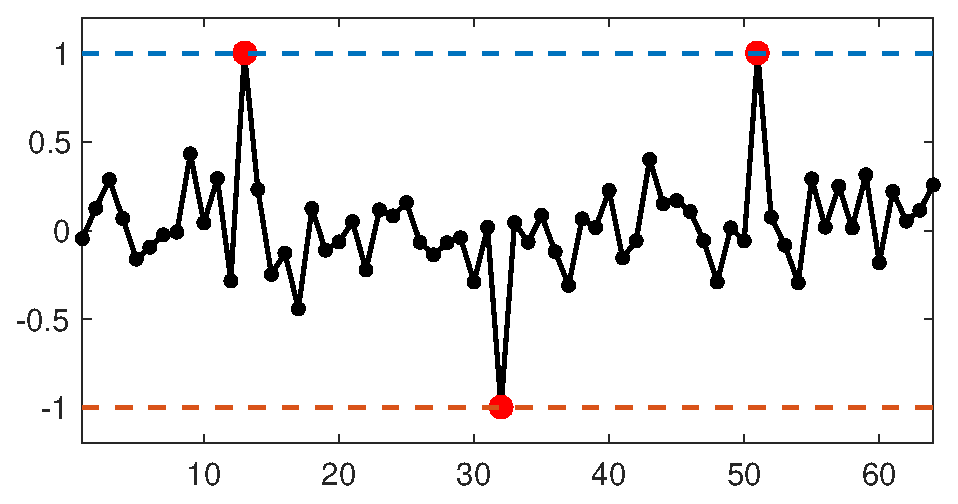
\includegraphics[width=.35\linewidth]{sparse-theory/certificates-cs/certif-cs-64}&
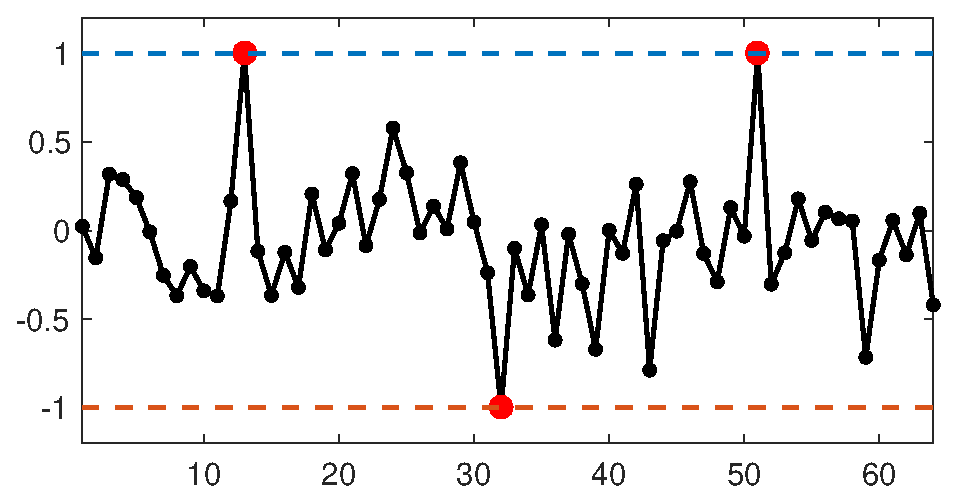
\includegraphics[width=.35\linewidth]{sparse-theory/certificates-cs/certif-cs-32}\\
$P=4$ & $P=8$ \\
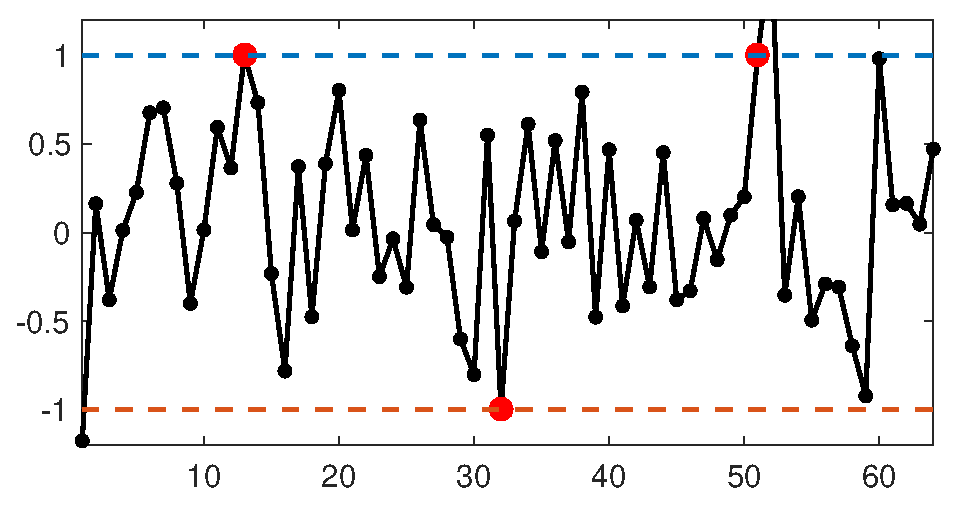
\includegraphics[width=.35\linewidth]{sparse-theory/certificates-cs/certif-cs-16}&
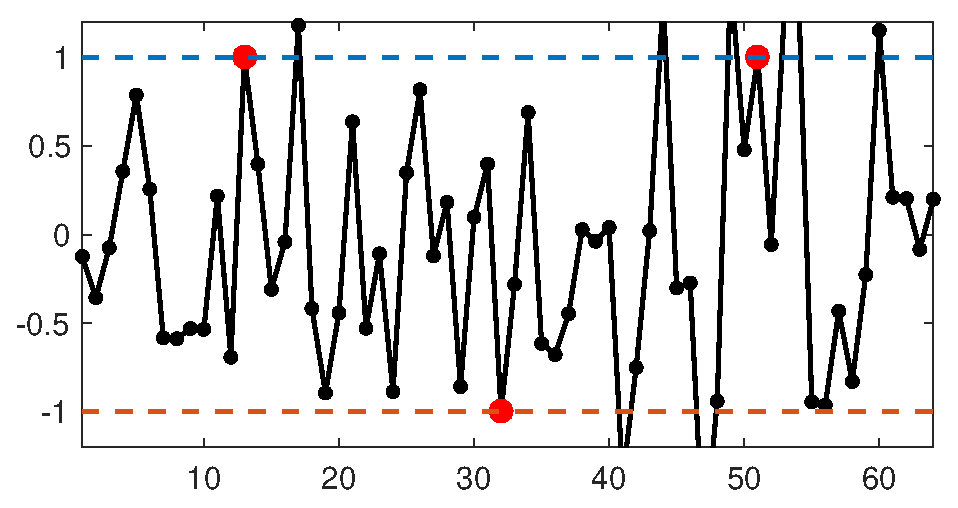
\includegraphics[width=.35\linewidth]{sparse-theory/certificates-cs/certif-cs-8}\\
$P=16$ & $P=32$
\end{tabular}
%%
\caption{\label{fig-certif-cs}
Display of certificate $\eta_F$ for a $A \in \RR^{p \times n}$, $n=64$, with independent Gaussian entries. 
}
\end{figure}

%%%%%%%%%%%%%%%%%%%%%%%%%%%%%%%%%%%%%%%%
%%%%%%%%%%%%%%%%%%%%%%%%%%%%%%%%%%%%%%%%
%%%%%%%%%%%%%%%%%%%%%%%%%%%%%%%%%%%%%%%%
\section{Sparse Deconvolution Case Study}

Chapter~\ref{chap-cs} studies the particular case where $A$ is random, in which case it is possible to make very precise statement about wether $\eta_F$ is a valid certificate.

Another interesting case study, which shows the limitation of this approach, is the case of ``super-resolution''. It corresponds to inverse problems where the columns $(a_i)_i$ of $A$ are highly correlated, since typically they are obtained by sampling a smooth kernel.

We thus consider the case where $a_i=\phi(z_i)$ where the $(z_i)_i \subset \XX$ is  a sampling grid of a domain $\XX$ and $\phi : \XX \rightarrow \Hh$ is a smooth map. One has 
\eq{
	A x = \sum_i x_i \phi(z_i).
}
Since we seek for sparse $x$, one can view $x$ as representing the weights of a discrete measure $m_{x} \eqdef \sum_{i=1}^N x_i \de_{z_i}$ where the dirac masses are constraint to be on the sampling grid.


The matrix $A$ is a discretized version of an infinite dimensional operator mapping Radon measures to vectors of observations $\Aa : m \in \Mm(\XX) \mapsto y = \Aa m \in \Hh$
\eq{
	\Aa(m) \eqdef \int_\XX \phi(x) \d m(x).
}
Indeed, one has for discrete measure $\Aa(m_x)=A x$. 

A typical example is when using $\Hh=L^2(\XX)$ with $\XX=\RR^d$ or $\XX=\TT^d$ and $\phi(z) = \tilde\phi(z-\cdot)$, which corresponds to a convolution
\eq{
	(\Aa m)(z) = \int \tilde\phi(z-x) \d m(x) = (\tilde \phi \star m)(z).
}
Note that here $\Hh$ is infinite dimensional, and to get finite dimensional observations, it suffices to sample the output and consider $\phi(z) = ( \phi(z-r_j) )_{j=1}^P$ (note that the observation grid $r \in \XX^P$ can be different from the recovery grid $z \in \XX^N$).




\begin{figure}
\centering
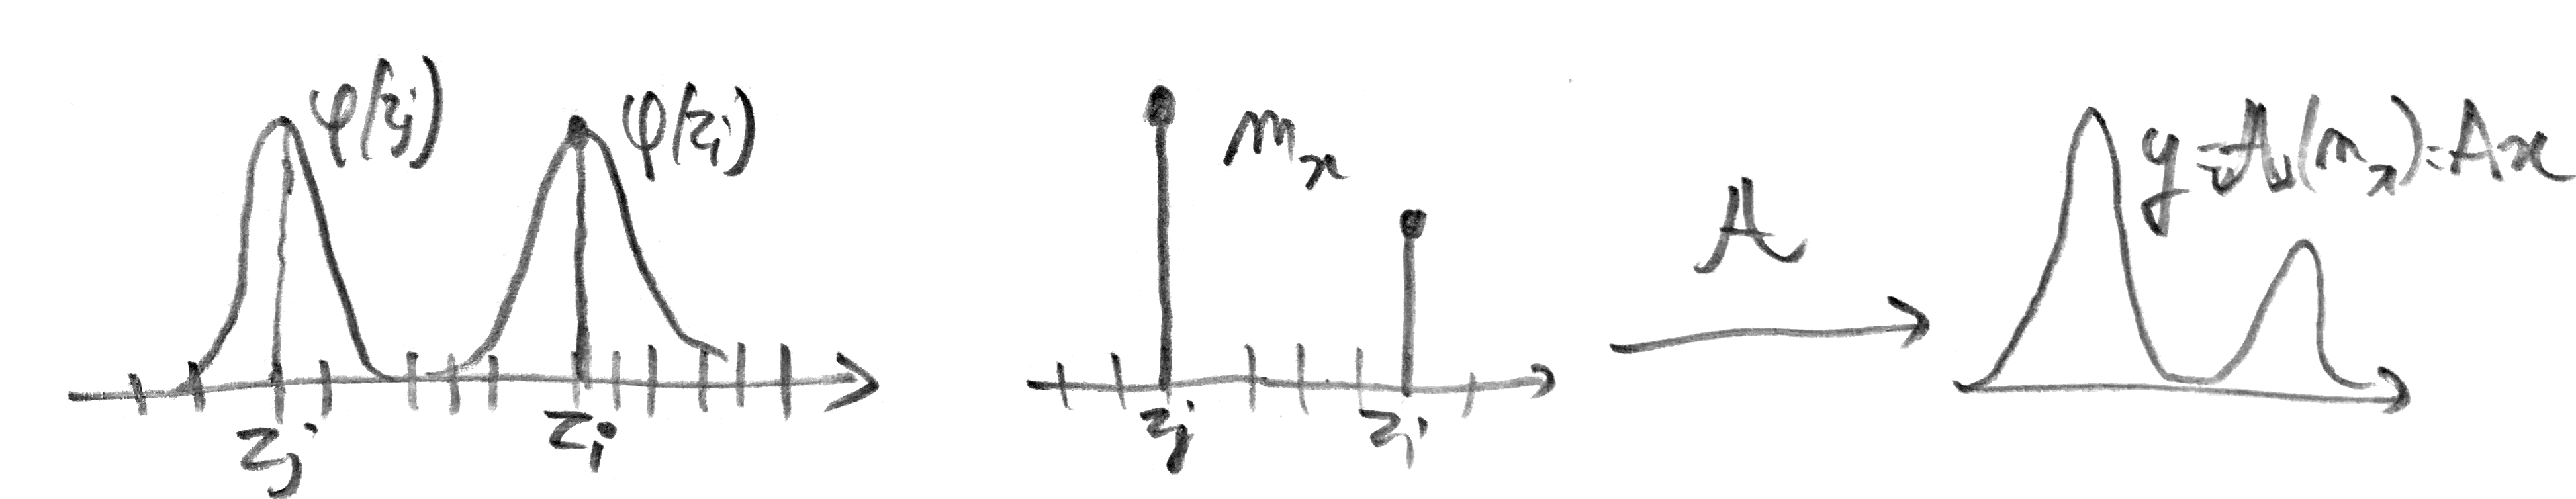
\includegraphics[width=.7\linewidth]{sparse-theory/proofs/spikes}
\caption{\label{fig-spikes}
Convolution operator. 
}
\end{figure}



Another example, actually very much related, is when using $\phi(z)=(e^{\imath k z})_{k=-f_c}^{f_c}$ on $\XX=\TT$, so that $\Aa$ corresponds to computing the $f_c$ low-frequencies of the Fourier transform of the measure
\eq{
	\Aa(m) = \pa{ \int_\TT e^{\imath k x} \d m(x) }_{k=-f_c}^{f_c}.
}
The operator $\Aa^*\Aa$ is a convolution against an ideal low pass (Dirichlet) kernel. By weighting the Fourier coefficients, one can this way model any low pass filtering on the torus.

Yet another interesting example on $\XX=\RR^+$ is the Laplace transform
\eq{
	\Aa(m) = z \mapsto \int_{\RR^+} e^{-x z} \d m(x).
}

We denote the ``continuous'' covariance as
\eq{
	\foralls (z,z') \in \XX^2, \quad
	\Cc(z,z') \eqdef \dotp{\phi(z)}{\phi(z')}_{\Hh}.
}
Note that this $\Cc$ is the kernel associated to the operator $\Aa^* \Aa$. 
%
The discrete covariance, defined on the computational grid is $C=(\Cc(z_i,z_i')))_{(i,i')} \in \RR^{N \times N}$, while its restriction to some support set $I$ is $C_{I,I}=(\Cc(z_i,z_i')))_{(i,i') \in I^2} \in \RR^{I \times I}$.

Using~\eqref{eq-eta-f-cov}, one sees that $\eta_F$ is obtained as a sampling on the grid of a ``continuous' ' certificate $\tilde\eta_F$
\eq{
	\eta_F = ( \tilde\eta_F(z_i) )_{i=1}^N \in \RR^N, 
}
\eql{\label{eq-etaf-cont}
	\qwhereq \tilde\eta_F(x) = \sum_{i \in I} b_i \Cc(x,z_i) \qwhereq b_I = C_{I,I}^{-1} \sign(x_{0,I}), 
}
so that $\eta_F$ is a linear combination of $I$ basis functions $(\Cc(x,z_i))_{i \in I}$. 

The question is wether $\norm{\eta_F}_{\ell^\infty} \leq 1$. If the gris is fine enough, i.e. $N$ large enough, this can only hold if $\norm{\tilde\eta_F}_{L^\infty} \leq 1$. The major issue is that $\tilde\eta_F$ is only constrained by construction to interpolate $\sign(x_{0,i})$ are points $z_{0,i}$ for $i \in I$. So nothing prevents $\tilde\eta_F$ to go outside $[-1,1]$ around each interpolation point. Figure~\ref{fig-certif-convol}�illustrates this fact. 


In order to guarantee this property of ``local'' non-degeneracy around the support, one has to impose on the certificate the additional constraint $\eta'(z_i)=0$ for $i \in I$. This leads to consider a minimum pre-certificate with vanishing derivatives 
\eql{\label{eq-minnorm-certif}
	\eta_V \eqdef A^* p_V
	\qwhereq p_V
	\uargmin{p \in L^2(\RR)} \enscond{\norm{p}_{L^2(\RR)}}{ \tilde\eta(z_I) = \sign(x_{0,I}), \tilde\eta'(z_I) = \zeros_I }.
}
where we denoted $\tilde\eta = \bar\psi \star p$. Similarly to~\eqref{eq-etaf-cont}, this vanishing pre-certificate can be written as a linear combination, but this time of $2|I|$ basis functions
\eq{
	\tilde\eta_V(x) = \sum_{i \in I} b_i \Cc(x,z_i) + c_i \partial_2\Cc(x,z_i), 
}
where $\partial_2\Cc$ is the derivative of $\Cc$ with respect to the second variable, and $(b,c)$ are solution of a $2|I| \times 2|I|$ linear system
\eq{
	\begin{pmatrix} b \\ c \end{pmatrix} 
	= 
	\begin{pmatrix}
		(\Cc(x_i,x_{i'}))_{i,i' \in I^2} & (\partial_2\Cc(x_i,x_{i'}))_{i,i' \in I^2} \\
		(\partial_1\Cc(x_i,x_{i'}))_{i,i' \in I^2} & (\partial_1\partial_2\Cc(x_i,x_{i'}))_{i,i' \in I^2}
	\end{pmatrix}^{-1}
	\begin{pmatrix} \sign(x_{0,I}) \\ \zeros_I \end{pmatrix} .
}
%
The associated continuous pre-certificate is $\tilde\eta_V=\bar\psi \star p_V$, and $\eta_V$ is a sampling on the grid of $\tilde\eta_V$.
%
Figure~\ref{fig-certif-cs}� shows that this pre-certificate $\eta_V$ is much better behaved than $\eta_F$. If $\norm{\eta_V}_\infty \leq 1$, one can apply~\eqref{thm-linrate-l1} and thus obtain a linear convergence rate with respect to the $\ell^2$ norm on the grid. But for very fine grid, since one is interested in sparse solution, the $\ell^2$ norm becomes meaningless (because the $L^2$ norm is not defined on measures). 
%
Since $\eta_V$ is different from $\eta_F$, one cannot directly applies Theorem~\ref{thm-support-stable}: the support is not stable on discrete grids, which is a fundamental property of super-resolution problems (as opposed to compressed sensing problems).
%
The way to recover interesting results is to use and analyze methods without grids. Indeed, after removing the grid, one can show that $\eta_V$ becomes the minimum norm certificate (and is the limit of $\eta_\la$). 




\begin{figure}
\centering
%%
\begin{tabular}{@{}c@{}c@{}}
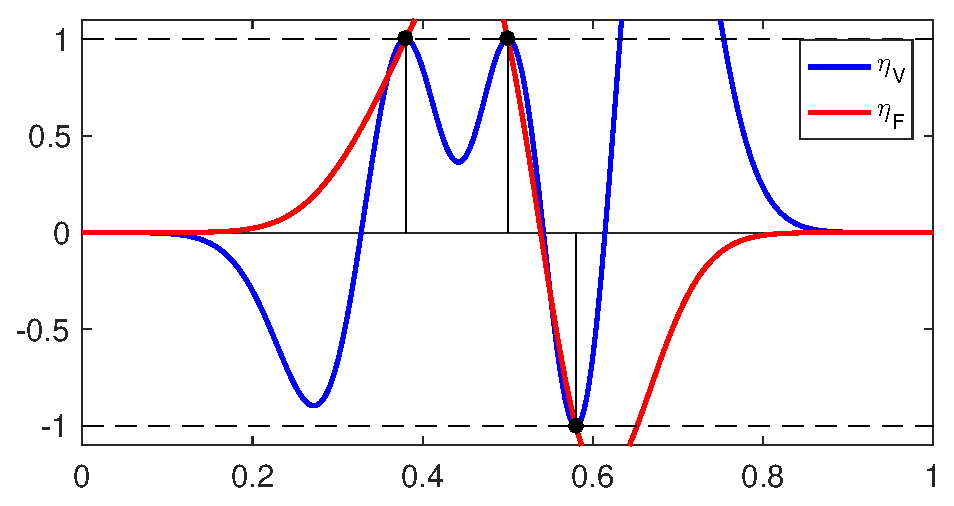
\includegraphics[width=.35\linewidth]{sparse-theory/certif-convol/etaV-N3-d40}&
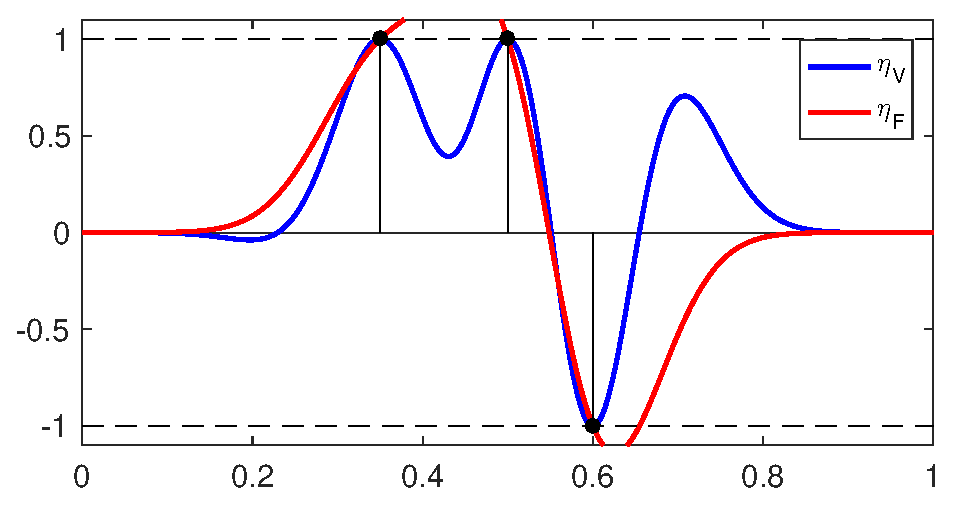
\includegraphics[width=.35\linewidth]{sparse-theory/certif-convol/etaV-N3-d50}\\
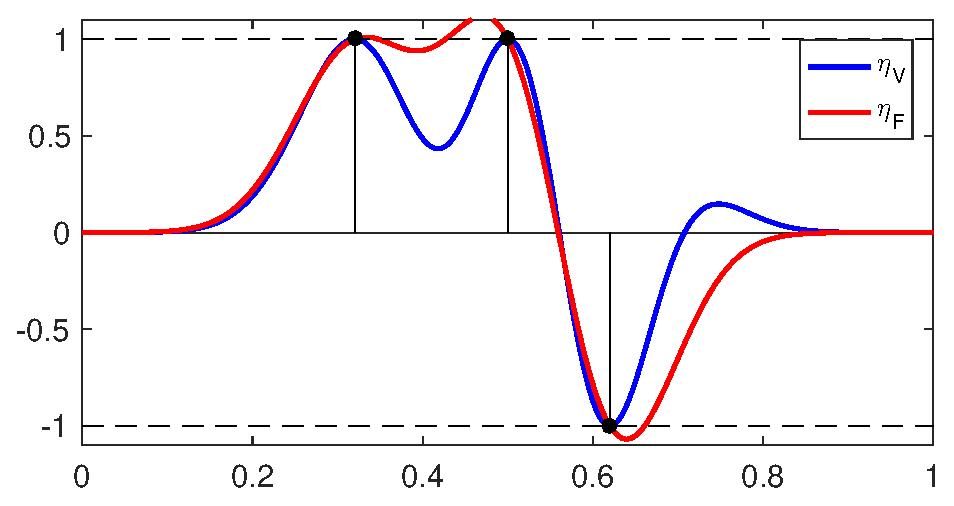
\includegraphics[width=.35\linewidth]{sparse-theory/certif-convol/etaV-N3-d60}&
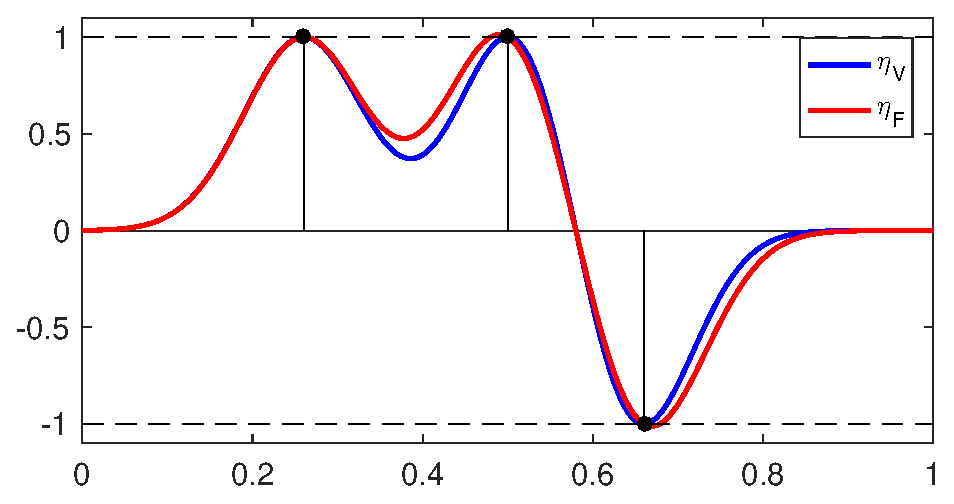
\includegraphics[width=.35\linewidth]{sparse-theory/certif-convol/etaV-N3-d80}
\end{tabular}
%%
\caption{\label{fig-certif-convol}
Display of ``continuous'' certificate $\eta_F$ and $\eta_V$ for $A$ being a convolution operator. 
}
\end{figure}

% !TEX root = ../FundationsDataScience.tex

\chapter{Compressed Sensing}
\label{chap-cs}

This chapter details an important class of inverse problems, which corresponds to using ``random'' forward operators $\Phi$. This is interesting from an applicative point of view since it allows to model a novel class of imaging devices which can potentially have improved resolution with respect to traditional operators (e.g. low-pass filters for usual cameras) when using in conjunction with sparse regularization technics. This is also interesting from a theoretical point of view, since the mathematical analysis becomes much simpler than with deterministic operators, and one can have good recovery and stability performances.
%
Let us however stress that the ``physical'' creation of hardware that fulfils the theoretical hypothesis, in particular in medical imaging, is still largely open (put aside some restricted areas), although the theory gives many insightful design guides to improve imaging devices.

The main references for this chapter are~\cite{mallat2008wavelet,foucart2013mathematical,scherzer2009variational}.

%%%%%%%%%%%%%%%%%%%%%%%%%%%%%%%%%%%%
%%%%%%%%%%%%%%%%%%%%%%%%%%%%%%%%%%%%
%%%%%%%%%%%%%%%%%%%%%%%%%%%%%%%%%%%%
\section{Motivation and Potential Applications}


%%%%%%%%%%%%%%%%%%%%%%%%%%%%%%%%%%%%
\subsection{Single Pixel Camera}

In order to illustrate the exposition, we will discuss the \guill{single pixel camera} prototype developed at Rice University~\cite{DuarteSinglePixel}, and which is illustrated by the figure~\ref{fig-single-pixel} (left).
%
It is an important research problem of developing a new class of cameras allowing to obtain both the sampling and the compression of the image. Instead of first sampling very finely (ie with very large $Q$) the analog signal $\tilde f$ to obtain a $f \in \RR^Q$ image then compressing enormously (ie with $M$ small) using~\eqref{eq-formule-thresh}, we would like to dispose directly of an economic representation $y \in \RR^P$ of the image, with a budget $P$ as close to $M$ and such that one is able to \guill{decompress} $y$ to obtain a good approximation of the image $f_0$.

The \guill{single-pixel} hardware performs the compressed sampling of an observed scene $\tilde f_0$ (the letter \guill{R} in Figure~\ref{fig-single-pixel}), which is a continuous function indicating the amount of light $\tilde f_0(s)$ reaching each point $s \in \RR^2$ of the focal plane of the camera.
%
To do this, the light is focused against a set of $Q$ micro-mirrors aligned on the focal plane. These micro-mirrors are not sensors. Unlike conventional sampling (described in Section~\ref{sec-sampling}), they do not record any information, but they can each be positioned to reflect or absorb light.
%
To obtain the complete sampling/compression process, one very quickly changes $P$ times the configurations of the micro-mirrors. For $p = 1,\dots, P$, one sets $\Phi_{p, q} \in \{0,1\}$, depending on whether the micromirror at position $q$ has been placed in the absorbing (0) or reflective (value 1) position at step $p$ of the acquisition.
%
The total light reflected at step $p$ is then accumulated into a single sensor (hence the name \guill{single pixel}, in fact it is rather a \guill{single sensor}), which achieves a linear sum of the reflected intensities to obtain the recorded $y_p \in \RR$ value.
%
In the end, if the light intensity arriving on the surface $c_q$ of the mirror indexed by $f_q = \int_{c_q} \tilde f_0(s) \text{d} s$ is denoted (as in the~\ref{sec-sampling} section) as $q$, the equation that links the discrete image $f \in \RR^Q$ \guill{seen through the mirrors} to the $P$ measures $y \in \RR^P$ is
\eq{
	\foralls p = 1,\ldots,P, \quad
	y_p \approx \sum_q \Phi_{p,n} \int_{c_n} \tilde f_0(s) \text{d} s = (\Phi f_0)_p, 
}
(here $\approx$ accounts for some noise), 
which corresponds to the usual forward model of inverse problems
\eq{
	y = \Phi f_0 + w \in \RR^P
}
where $w$ is the noise vector. 
%
It is important to note that the mirrors do not record anything, so in particular the $f_0$ discrete image is never calculated or recorded, since the device directly calculates the compressed representation $y$ from the analog signal $\tilde f_0$.
%
The term $w$ models here the acquisition imperfections (measurement noise). The compressed sampling therefore corresponds to the transition from the observed scene $\tilde f_0$ to the compressed vector $y$. The \guill{decompression} corresponds to the resolution of an inverse problem, whose goal is to find a good approximation of $f_0$ (the discrete image \guill{ideal} as seen by the micro-mirrors) from $y$.

\begin{figure} \centering
\begin{tabular}{@{}c@{\hspace{1mm}}c@{\hspace{1mm}}c@{}}
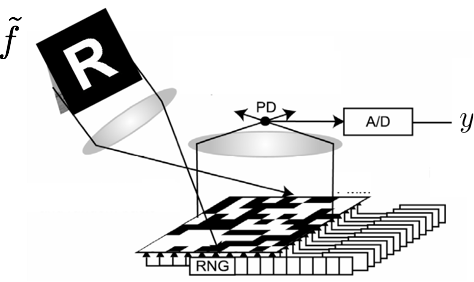
\includegraphics[width=.45\linewidth]{cs/single-pixel/single-pixel-schema}&

\includegraphics[width=.25\linewidth]{cs/single-pixel/reconstruction-1}&
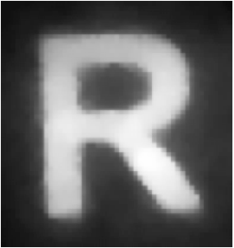
\includegraphics[width=.25\linewidth]{cs/single-pixel/reconstruction-6}\\
Diagram of the device & $f$ & $f^\star$, $P/Q = 6$
\end{tabular}
\caption{Left: diagram of the single-pixel acquisition method.
%
Center: image $f_0 \in \RR^Q$ \guill{ideal} observed in the focal plane of the micro-mirrors.
%
Right: image $f_0^\star = \Psi x^\star$ reconstructed from observation $y \in \RR^P$ with a compression factor $P / Q = 6$ using $\ell^1$-type regularization.
\label{fig-single-pixel}}
\end{figure}


%%%%%%%%%%%%%%%%%%%%%%%%%%%%%%%%%%%%
\subsection{Sparse Recovery}

In order to reconstruct an approximation of the (unknown) image $f_0$, following Section~\ref{sec-sparse-ip}, we assume it is sparse in some dictionary $\Psi$. Denoting $A \eqdef \Psi \Phi \in \RR^{P \times N}$, this leads us to consider the usual $\ell^1$ regularized poblem~\eqref{eq-lasso-lagr-ip}
\eql{\label{eq-lasso-lagr-ip-cs}\tag{$\Pp_\la(y)$}
	x_\la \in \uargmin{x \in \RR^Q} \frac{1}{2\la} \norm{y-Ax}^2 + \norm{x}_1, 
} 
so that the reconstructed image is $f_\la = \Psi x_\la$. We also sometimes consider the constraint problem
\eql{\label{eq-lasso-lagr-constr-cs}\tag{$\Pp^\epsilon(y)$}
	x_\epsilon \in \uargmin{\norm{Ax-y} \leq \epsilon} \norm{x}_1, 
} 
where, for the sake of simplicity, we set $\epsilon=\norm{w}$ (which we assume is known). From a mathematical point of view, these problem are equivalent in the sense that there exists a bijection between $\la$ and $\epsilon$ which links it solution. But in practice, this bijection is not explicitly known and depends on $y$.  

Here, it is important to remember that $A$ is drawn from a random matrix ensemble. For an arbitrary $\Psi$, it is hard to analyze this random distribution. If $\Psi$ is orthogonal, and the distribution of the columns of $\Phi$ are invariant by rotation (which is the case if the entries are i.i.d. Gaussian), then $A$ has the same distribution as $\Phi$. In the following, we thus directly models the distribution of $A$ and assumes it has some nice property (typically it is close to being Gaussian i.i.d.). 

%%%%%%%%%%%%%%%%%%%%%%%%%%%%%%%%%%%%
%%%%%%%%%%%%%%%%%%%%%%%%%%%%%%%%%%%%
%%%%%%%%%%%%%%%%%%%%%%%%%%%%%%%%%%%%
\section{Dual Certificate Theory and Non-Uniform Guarantees}
\label{sec-cs-certif}

%%%%%%%%%%%%%%%%%%%%%%%%%%%%%%%%%%%%
\subsection{Random Projection of Polytopes}

When there is no noise, $w=0$ a way to tackle the problem is to use the caracterization of solutions of $(\Pp^0(Ax_0))=(\Pp_0(Ax_0))$ given in Section~\ref{sec-polytope-proj}. According to Proposition~\ref{prop-polytope-proj}, identifiable vectors with sparsity $\norm{x_0}_0=s$ corresponds to $s$-dimensional faces of the $\ell^1$ balls $B_1$ which are mapped to face of the projected polytope $AB_1$. This leads to a combinatorial problems to count the number of face of random polytope. Donoho and Tanner were able to perform a sharp analysis of this problem. They showed the existence of two regimes, using two functions $C_A, C_M$ so that, with high probability (i.e. a probability converging exponentially fast to $1$ with $(n,p)$) on the matrix $A$
\begin{rs}
	\item All $x_0$ so that $\norm{x_0}_0 \leq C_A(P/N)P$ are identifiable.
	\item Most $x_0$ so that $\norm{x_0}_0 \leq C_M(P/N)P$ are identifiable.
\end{rs}
For instance, they show that $C_A(1/4)=0.065$ and $C_M(1/4)=0.25$. Figure~\ref{fig-phase-trans} illustrates numerically these two phase transitions. 
%
This analysis can be shown to be sharp in high dimension, i.e. when $\norm{x_0}_0 > C_M(P/N)P$, then $x_0$ is not identifiable with high probability (this corresponds to a phase transition phenomena). 
%
For large dimensions $(N,P)$, the scaling given by $C_M$ describe very well what one observe in practice. For $P=N/4$ (compression of a factor $4$), one retrieve in practice all vector with sparsity smaller than $P/N$. 
%
The function $C_M$ can be computed numerically, and it can be shown to have a logarithmic grows $C_M(r) \sim \log(r)$ for small $r$. This suggests that for high compression regime, one recovers with $\ell^1$ minimization almost all vector with a sparsity $\norm{x_0}_0$ proportional (up to log factor) to the number of measurements $P$. 


%%%%%%%%%%%%%%%%%%%%%%%%%%%%%%%%%%%%
\subsection{Random Matrices}
\label{sec-random-matrix}

The analysis of the performance $\ell^1$ minimization to solve compressed sensing problem is made possible because of the very precise understanding of the distribution of the singular values of certain random ensemble let us illustrate this in the Gaussian case, which is the simplest, and is very illustrative. 

An important part of the recovery proof relies on controlling the correlation matrix $A_I^*A_I$ of selected columns, and even more importantly, its inverse $(A_I A_I)^{-1}$. Such a matrix $B=A_I$ is of size $(P,s)$ and is also drawn from the Gaussian ensemble. 
%
Fixing $s$ and letting $P \rightarrow +\infty$, one has thanks to the low of large numbers $B^*B \rightarrow \Id_s$ almost surely. This is however not a very realistic setting, since in general, one hope to have $s$ almost equal, up to log factor, to $P$.

%%%
\paragraph{Linear growth $P = s/\be$. }

A quite extreme setting is when $s$ grows proportionally to $P$, and impose $s/P = \be$. 
%
In this case, the eigenvalues of $B^*B$ are, for large $p$, essentially contained in the interval $[\la_-,\la_+]$
where $\la_\pm=(1 \pm \sqrt{\be})^2$, $\be \eqdef p/s$, in the sense that the probability distribution of eigenvalues converges (in the weak sense of measures) toward the Marcenko-Pastur law
\eq{
	\foralls (u,v) \in \RR_+^2, \quad
		\PP( \text{eig}(B^\top B) \in [u,v] ) \overset{p \rightarrow +\infty}{\longrightarrow} \int_u^v f_\be(\la) \d \la
}
where one fix the ratio $\be=s/P$, and the Marcenko-Pastur law is
\eq{
	f_\be(\la) \eqdef \frac{1}{2\pi\be \la} \sqrt{ (\la-\la_-)_+(\la_+-\la) } 1_{[\la_-,\la_+]}(\la).
}
Figure~\eqref{fig-marcenko-pastur} illustrates this convergence. 

\begin{figure}
\centering
%%
\begin{tabular}{@{}c@{\hspace{5mm}}c@{}}
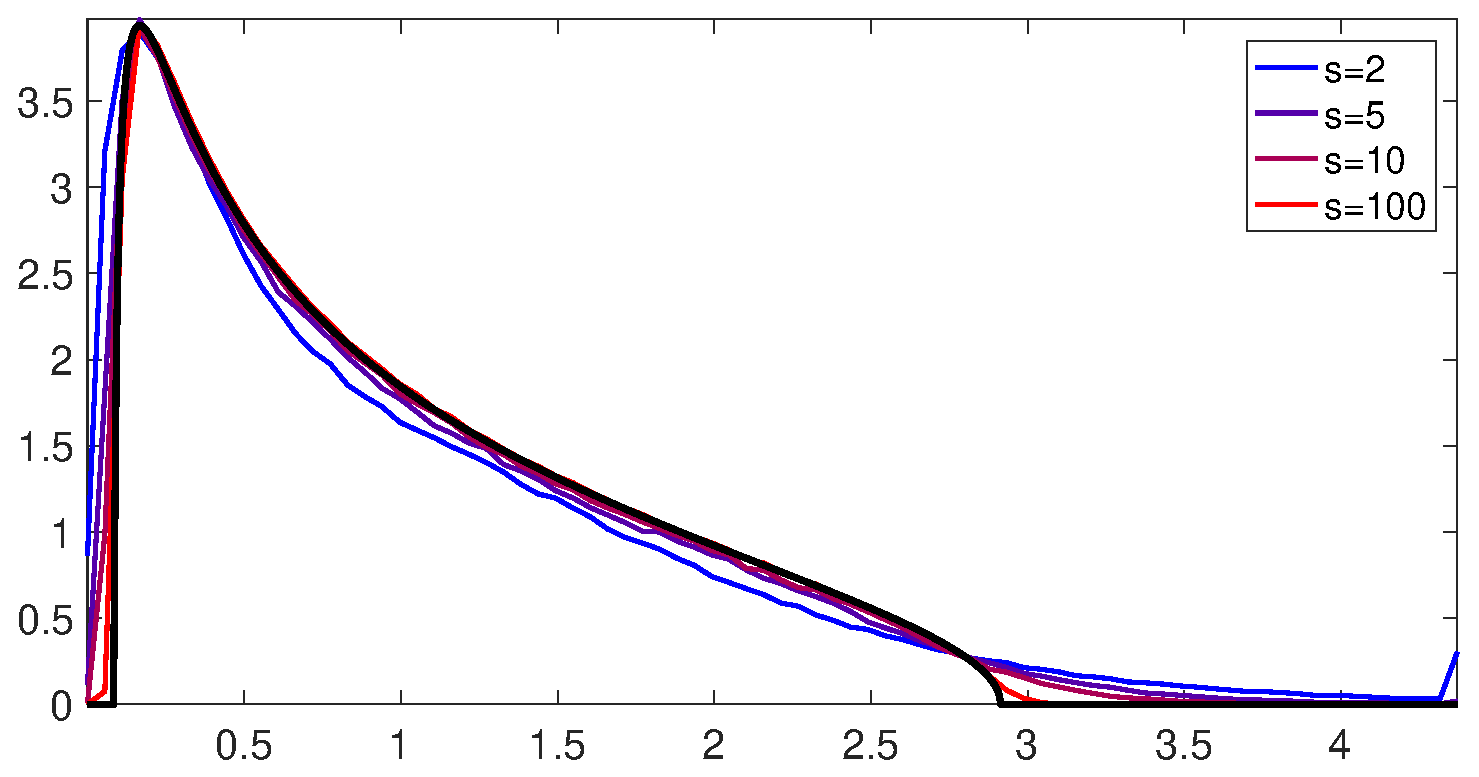
\includegraphics[width=.4\linewidth]{cs/marcenko-pastur/marcenko-pastur-2}&
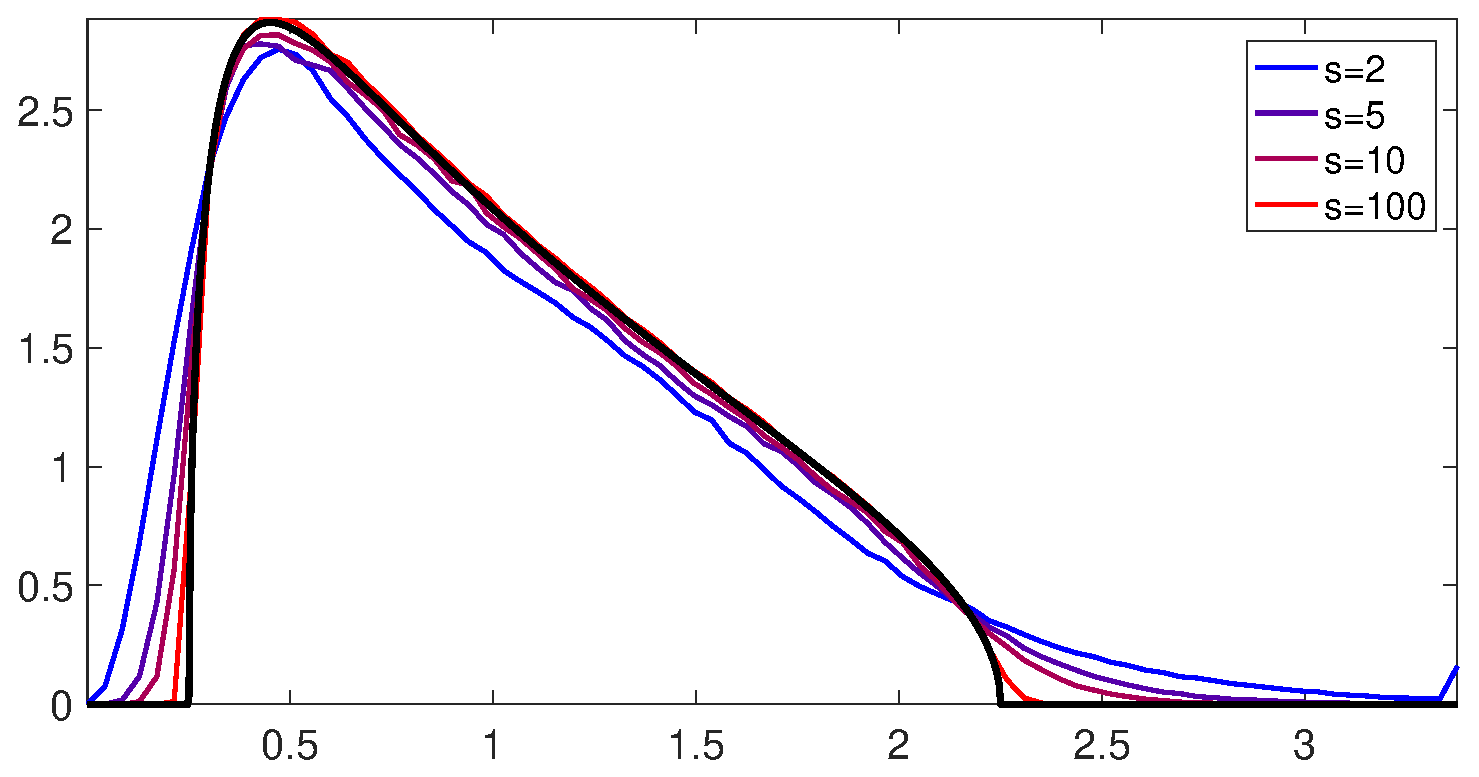
\includegraphics[width=.4\linewidth]{cs/marcenko-pastur/marcenko-pastur-4}\\
$\be=1/2$ & $\be=1/4$ \\
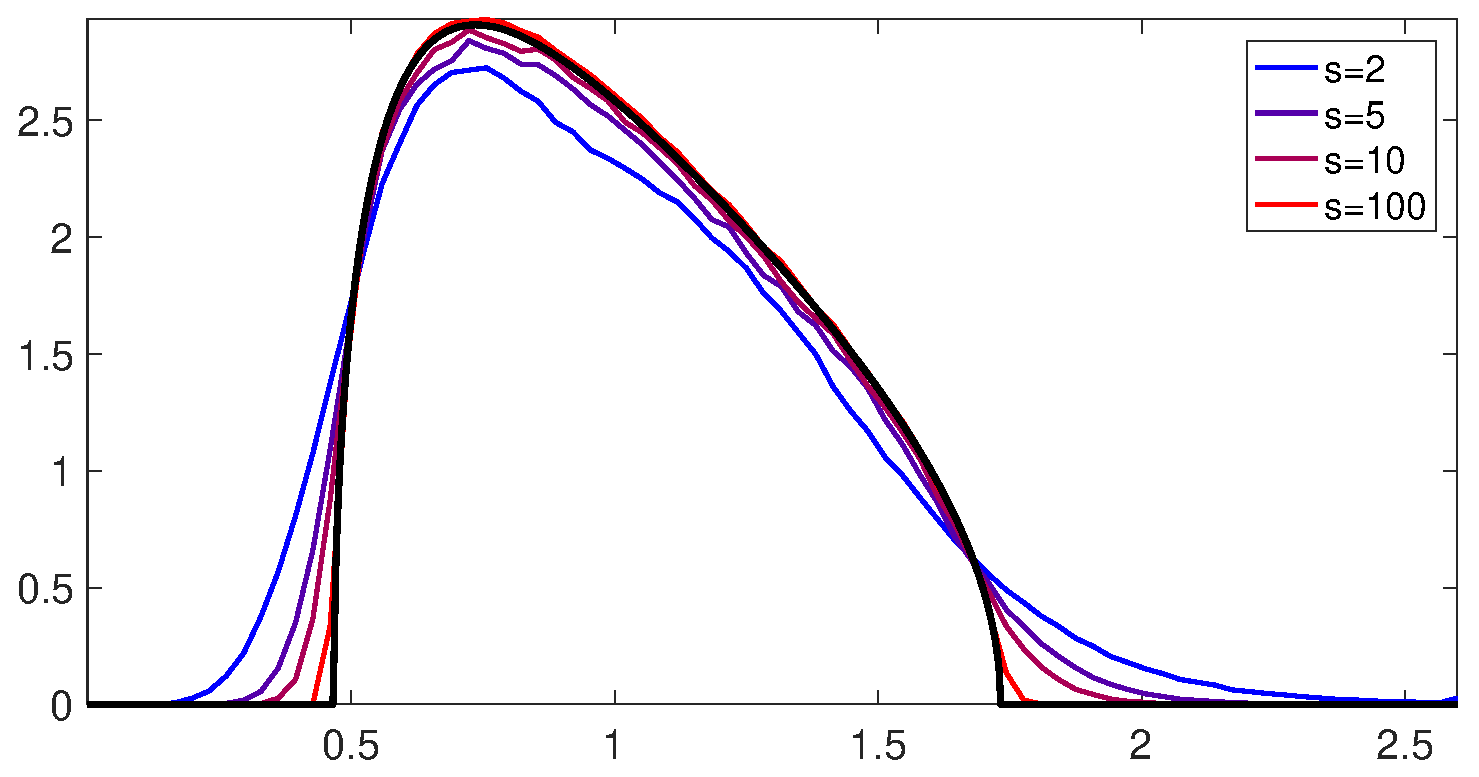
\includegraphics[width=.4\linewidth]{cs/marcenko-pastur/marcenko-pastur-10}&
\includegraphics[width=.4\linewidth]{cs/marcenko-pastur/marcenko-pastur-50}\\
$\be=1/10$ & $\be=1/50$ 
\end{tabular}
%%
\caption{\label{fig-marcenko-pastur}
Illustration of the convergence toward the Marcenko-Pastur law.
}
\end{figure}



\begin{figure}
\centering
\includegraphics[width=.5\linewidth]{cs/marcenko-pastur/mp-laws.eps}
%%
\caption{\label{fig-marcenko-pastur}
Display of the Marcenko-Pastur distribution $f_\be$ for various $\be$.
}
\end{figure}


%%%
\paragraph{Super-linear grows $P = s \log(\ldots)$. }

In order to have a better concentration of the singular values of $A_I^* A_I$ around $1$, one needs to have a slightly super-linear growth of $P$ with $s$. In this setting one has that $A_I^* A_I$. In order to derive non-asymptotic (i.e. with explicit constants) results, one can use a celebrated concentration inequality due to Talagrand, which assert that one has a fast concentration of this randomized covariance $A_I^* A_I$ toward its expectation $\Id_s$.
\eql{\label{eq-talagrand}
	\PP\pa{ \norm{ A_I^* A_I - \Id_s }_{\text{op}} \geq t + \sqrt{\frac{s}{P}} } \leq e^{ -\frac{t^2s}{2} }. 
}

%%%%%%%%%%%%%%%%%%%%%%%%%%%%%%%%%%%%
%\subsection{Gaussian Width}

% For Gaussian matrices (or at least rotation invariant distributions).

%%%%%%%%%%%%%%%%%%%%%%%%%%%%%%%%%%%%
\subsection{Dual Certificates}

In order to analyze recovery performance, one can looks not only for $\ell^2$ stability ($\norm{x_\la-x_0} \sim \norm{w}$) but also that $x_\la$ has the same support as $x_0$ when $\norm{w}$ is small. As detailed in Section~\ref{sec-sparsistency}, this requires to  ensure that the pre-certificate $\eta_F$ defined in~\eqref{eq-minnorm-certif} is non-degenerated, i.e.
\eql{\label{eq-cond-fuchs}
	\norm{\eta_F}_\infty \leq 1 
	\qwhereq 
	\eta_F = A^* A_I (A_I^*A_I)^{-1} \sign(x_{0,I}).
}
Figure~\ref{fig-certif-cs} suggests that this should be the case if $P$ is large enough with respect to $\norm{x_0}$. This theorem backup this observation.


%%%%%%
\paragraph{Coherence-based analysis.}

We first perform a crude analysis using the so-called coherence of the matrix $A=(a_j)_{j=1}^N$ where the $a_j \in \RR^P$ are the columns of $A$, which we assume to be normalized $\norm{a_j}=1$
\eql{
	\mu \eqdef = \umax{0 \leq i \neq j } |\dotp{a_i}{a_j}| = \norm{A^*A-\Id_N}_\infty
}
where $\norm{C}_\infty=\max_{i,j} |C_{i,j}|$.
%
The coherence is $0$ for an orthogonal matrix, and is always larger than $1$, $\mu \in [0,1]$. 
%
The smaller the coherence, the better conditioned the inverse problem $Ax=y$ is, and the more likely is the certificate $\eta_F$ to be non-degenerate, as shown by the following proposition.

\begin{prop}\label{prop-bound-coh}
	One has, denoting $s=\norm{x_0}_0=|I|$ where $I=\supp(x_0)$, for $\mu < \frac{1}{s-1}$, 
	\eql{\label{eq-coh-bound}
		\norm{\eta_{F,I^c}}_\infty \leq \frac{ s\mu }{ 1-(s-1)\mu }.
	}
	In particular, if $s < \frac{1}{2}\pa{ 1+\frac{1}{\mu} }$, $\norm{\eta_{F,I^c}}_\infty < 1$ and one can thus apply the 
	recovery Theorem~\ref{thm-support-stable}. 
\end{prop}
\begin{proof}
	We recall that the $\ell^\infty$ operator norm (see Remark~\ref{rem-operator-norm}) is
	\eq{
		\norm{B}_\infty = \umax{i} \sum_j |B_{i,j}|.
	}
	We denote $C=A^*A$. One has
	\eq{
		\norm{A_{I^c}^*A_I}_\infty = \umax{j \in I^c} \sum_{i \in I} C_{i,j} \leq s \mu
		\qandq
		 \norm{  \Id_s - A_I^*A_I }_\infty = \umax{j \in I} \sum_{i \in I, i \neq j} C_{i,j} \leq (s-1) \mu
	}
	One also has 
	\begin{align*}
		\norm{(A_I^*A_I)^{-1}}_\infty &= \norm{( (\Id_s - A_I^*A_I) - \Id_s)^{-1}}_\infty
		= \norm{ \sum_{k \geq 0} (\Id_s - A_I^*A_I)^k }_\infty \\
		&\leq \sum_{k \geq 0} \norm{  \Id_s - A_I^*A_I }_\infty^k \leq \sum_{k \geq 0} ((s-1) \mu)^k = \frac{1}{1 - (s-1)\mu}
	\end{align*}
	which is legit because the matrix series indeed converge since $(s-1)\mu<1$.
	%
	Using these two bounds, one has
	\eq{
		\norm{\eta_{F,I^c}}_\infty = 
		\norm{A_{I^c}^* A_I (A_I^*A_I)^{-1} \sign(x_{0,I})}_\infty
		\leq 
		\norm{A_{I^c}^* A_I}_\infty 
		\norm{(A_I^*A_I)^{-1}}_\infty 
		\norm{\sign(x_{0,I})}_\infty 
		\leq 
		(s \mu) \times \frac{1}{1 - (s-1)\mu} \times 1.
	}
	%
	One has 
	\eq{
		\frac{ s\mu }{ 1-(s-1)\mu } \quad\Longleftrightarrow\quad
		2s\mu < 1+\mu
	}
	which gives the last statement.
\end{proof}

Note that this proof actually shows that if  $s < \frac{1}{2}\pa{ 1+\frac{1}{\mu} }$, all certificate $\eta_F$ are valid, for any sign pattern $\sign(x_0)$. This actually implies a much stronger stability in the sense that whatever the noise $w$ (which might not be small), the support of $x_\la$ is included (not necessarily equal) in the one of $x_0$.

One can show that one always has
\eql{\label{eq-bound-cohe-mat}
	\mu \geq \sqrt{\frac{N-P}{P(N-1)}}.
}
For Gaussian matrix $A \in \RR^{P \times N}$, one has for large $(N,P) \rightarrow +\infty$
\eq{
	\mu \sim \sqrt{ \log(PN) / P }
}
which shows that Gaussian matrix are close to being optimal for the bound~\eqref{eq-bound-cohe-mat} if $N \gg P$.
%
Applying Proposition~\ref{prop-bound-coh} thus shows that $\ell^1$ regularization is able to recover with a stable support vector with less than $s \sim O(\sqrt{P})$ (ignoring log terms) non-zero coefficients. In face, we will show now that it does much better and recover a proportional number $s \sim O(P)$. This is because the coherence bound~\eqref{eq-coh-bound} is very pessimistic.

%%%%%%
\paragraph{Randomized analysis of the Fuchs certificate.}

We consider here a class of sufficiently ``random'' matrices. 

\begin{defn}[sub-Gaussian random matrix]
A random matrix $\sqrt{P}�A$ is said to be sub-Gaussian if its entries are independent such that $\EE(A_{i,j})=0$ (zero mean) $\EE(A_{i,j}^2)=1/P$ and 
\eq{\label{eq-sub-gaussian}
	\PP(|\sqrt{P}�A_{i,j}| \geq t) \leq \be e^{-\kappa t^2}. 
}
Note that its entries does not needs to be identically distributed, but the sub-Gaussiannity parameter $(\be,\kappa)$ should not depend on $(i,j)$. 
%
Note also the presence of the normalization factor $\sqrt{P}$, which is here to ensure $\EE(\norm{a_j}^2)=1$ where $a_j$ are the columns of $A$.
\end{defn}

Typical example of sub-Gaussian random matrix are Gaussian or Bernoulli matrices. 


\begin{thm}\label{thm-cs-etaf}
	For a given $x_0 \in \RR^N$, denoting $s=\norm{x_0}_0$, and assuming $A$ is sub-Gaussian, then for for any $0 < \epsilon < 1$ provided that
	\eq{
		P \geq \frac{4c}{1-\de} s \log(2N/\epsilon)
		\qwhereq
		\de^2 \eqdef \frac{C}{4c} \pa{ \frac{7}{\log(2N/\epsilon)}+\frac{2}{s} }
	}
	condition~\eqref{eq-cond-fuchs} holds with probability $1-\epsilon$, 
	so that $x_\la$ has the same support and sign as $x_0$ when $(\norm{w}, \norm{w}/\la)$ is small enough.
	% 
	The constant $C,c$, $C=\frac{2}{3\tilde c}$ where $\tilde c \eqdef \frac{\kappa^2}{4\be+2\kappa}$ only depends on the sub-Gaussianity parameter $(\be,\kappa)$ appearing~\eqref{eq-sub-gaussian}, and for Gaussian or Benoulli matrices, $c=1/2$.
\end{thm}

\begin{proof}
	We only give the main insight for the proof. Its crux relies on the fact that $\norm{A_{I^c}^* p_F}_\infty \leq 1$ reads
	\eq{
		\umax{j \notin I} |\dotp{a_j}{p_F}| \leq 1
	}
	where $p_F = A_I^{*+} s_{0,I}$ is \textit{independent} from the vectors $(a_j)_{j \notin I}$ it is correlated against. 
	%
	This allows one to check this condition by first controlling $\norm{p_F}$ and then making as if $p_F$ was a fixed deterministic vector. 
	%
	Noticing 
	\eq{
		\norm{p_F}^2 = \dotp{ A_I (A_I^*A_I)^{-1} s_{0,I} }{ A_I (A_I^*A_I)^{-1} s_{0,I} }
		= \dotp{(A_I^*A_I)^{-1} s_{0,I}}{s_{0,I}}, 
	}
	the heuristic reasoning is that, following what we said in Section~\eqref{sec-random-matrix}, if $P$ grows slightly (logarithmically) faster than $s$, $A_I^*A_I$ is close to $\Id_s$ (see Talagrand inequality�~\eqref{eq-talagrand}), so that 
	\eql{\label{eq-estimate-pf-norm}
		\norm{p_F}^2 \sim \norm{s_{0,I}}^2 = s
	}
	For a \textit{fixed} $p_F$, one has that $\dotp{a_j}{p_F}$ is Gaussian distributed with variance $\norm{p_F}^2/P$, and 
	we use the well known fact (already encountered for denoising using thresholding) that the maximum of $P-s$ such vectors concentrates just bellow the universal threshold $\norm{p_F}\sqrt{2 \log(N-s)/P}$. Using the estimate~\eqref{eq-estimate-pf-norm}, one sees that $\norm{p_F}_\infty \leq 1$ is implied by $2\log(N)s/P \leq 1$, which gives the sharp scaling $P \geq 2\log(N) s$. 
	
	In order to get robustness to noise, one needs to impose that $\norm{A_{I^c}^* p_F} < 1$, which can be achieve by using a slightly stronger scaling  $P \geq 2(1+\de)\log(N) s$ for a small $\de$.
	
	One can actually make this reasoning very precise, because quite surprisingly, it turns out that $ps/\norm{p_F}^2$ is actually distributed according to a $\chi^2$ variable with $P-s+1$ degree of freedom (i.e. the sum of $P-s+1$ squares of Gaussian variables). Since one has a very good understanding of the clustering of such a $\chi^2$ variable around its means, one can thus show that $\norm{p_F} \leq (1-\de) \sqrt{s}$ with high precision for arbitrary small $\de>0$.
\end{proof}


\begin{figure}
\centering
%%
\includegraphics[width=.6\linewidth]{cs/max-gaussian/max-gaussian}
%%
\caption{\label{fig-max-gaussian}
Graphical display of how the maximum of $N$ i.i.d. gaussians concentrates tightly just bellow the $\sqrt{2\log(N)}$ dashed curve. 
}
\end{figure}
 
For $(N,s) \rightarrow +\infty$, one has $\de \rightarrow 0$, so that informally, the scaling is 
\eql{\label{eq-etaf-gaussiancase}
	P \geq 2s \log(2N/\epsilon).
}
This theorem states a non-uniform recovery guarantee, in the sense that one first choose a vector $x_0$, \text{then} draws the matrix $A$, and the recovery results holds with high probability. This should be contrasted with the RIP theory developed in Section~\ref{sec-rip} which provides stronger uniform guarantees.


\begin{figure}
\centering
%%
\begin{tabular}{@{}c@{}c@{}c@{}}
\includegraphics[width=.35\linewidth]{cs/phase/phase-transition-1}&
\includegraphics[width=.28\linewidth]{cs/phase/phase-transition-2}&
\includegraphics[width=.35\linewidth]{cs/phase/phase-transition-crit}
\end{tabular}
%%
\caption{\label{fig-phase-trans}
Phase transitions. For the figure on the right shows probability as function of sparsity that certain criteria hold true, 
blue: w-ERC,  black: ERC, green $|\eta_F| \leq 1$, red: identifiability. 
}
\end{figure}



%%%%%%%%%%%%%%%%%%%%%%%%%%%%%%%%%%%%
%%%%%%%%%%%%%%%%%%%%%%%%%%%%%%%%%%%%
%%%%%%%%%%%%%%%%%%%%%%%%%%%%%%%%%%%%
\section{RIP Theory for Uniform Guarantees}
\label{sec-rip}

%%%%%%%%%%%%%%%%%%%%%%%%%%%%%%%%%%%%
\subsection{RIP Constants}

The RIP constant $\de_s$ of a matrix $\Phi \in \RR^{P \times N}$ is defined as
\eql{\label{eq-rip}
	\foralls z \in \RR^N, \quad
	\normz{z} \leq s \qarrq
	(1-\de_{s}) \norm{z}^2 \leq \norm{\Phi z}^2 \leq (1+\de_{s}) \norm{z}^2 
}

\begin{figure}
\centering
%%
\begin{tabular}{@{}c@{\hspace{5mm}}c@{}}
\includegraphics[width=.25\linewidth]{cs/rip-const/delta-k}&
\includegraphics[width=.55\linewidth]{cs/rip-const/eigen-distrib}
\end{tabular}
%%
\caption{\label{fig-rip-const}
Left: evolution of lower bounds $\hat \de_k$ on the RIP constant. Right: empirical distribution of singular values of Gaussian matrices.
}
\end{figure}

The following theorem states that for a sub-Gaussian random matrix, these RIP constant grows slowly with $s$.
%
Let us stress that, although this is an abuse of notation, here we assume that $A$ is a random matrix, and not a deterministic one as previously considered. 

\begin{thm}\label{thm-rip-random}
	If $A$ is a sub-Gaussian random matrix, then provided
	\eql{
		P \geq C \de^{-2} s \ln(eN/s)
	}
	it satisfies $\de_s \leq 1$ with probability $1 - 2e^{ -\de^2 \frac{m}{2C} }$, where $C$ only depends on the sub-Gaussianity parameters appearing in~\eqref{eq-sub-gaussian}.
\end{thm}


We do not prove this Theorem, and simply give the main intuition. 
%
The proof of this theorem relies on results regarding the distribution of the singular values of Gaussian matrices. Indeed, the RIP condition~\eqref{eq-rip} is equivalent to having the bound $\text{eig}( A_I^* A_I ) \subset [1-\de_s,1+\de_s]$ for all Gaussian matrices $A_I$ extracted from $A$. 
%
In the Gaussian case (actually this holds for any random matrix with i.i.d. entries and unit covariance), one has a very good understanding of the distribution of the singular values of covariance matrices $B^*B \in \RR^{s \times s}$ of a Gaussian matrix $B$ of size $(P,s)$, $B \sim \texttt{randn}(P,s)/\sqrt{P}$, as detailed in Section~\ref{sec-random-matrix}.  In particular, using Talagrand concentration inequality~\eqref{eq-talagrand}, one obtains the desired controls over the $\de_s$ constants. 



%%%%%%%%%%%%%%%%%%%%%%%%%%%%%%%%%%%%
\subsection{RIP implies stable recovery}

In the following, we fixe a vector $x \in \RR^N$ and denote $y=\Phi x + w$ the measurement, with $\norm{w} \leq \epsilon$. We denote $\bar x_s \in \RR^N$ the best $s$-term approximation of $x$, obtained by only keeping the $s$ largest coefficients in magnitude from $x$ and setting the others to 0.

We consider a solution $x^\star$ of
\eq{
	\umin{\norm{\Phi \tilde x - y} \leq \epsilon} \normu{\tilde x}. 	
}
This note recall the proof from~\cite{candes-cras} of the following theorem

\begin{thm}[\cite{candes-cras}]\label{thm-rip}
	If $\de_{2s} \leq \sqrt{2}-1$ then there exists $C_0, C_1$ such that
	\eq{
		\normu{x^\star-x_0} \leq \frac{C_0}{\sqrt{s}}\norm{\bar x_s-x_0} + C_1 \epsilon.
	}
\end{thm}

Putting together Theorems~\ref{thm-rip-random}�and~\ref{thm-rip} gives the following recovery guarantee.

\begin{thm}\label{thm-rip-final}
	If $A$ is a sub-Gaussian random matrix, then provided
	\eql{\label{eq-thm-rip-final}
		P \geq C \de^{-2} s \ln(eN/s)		
	}
	with probability $1 - 2e^{ -\de^2 \frac{P}{2C} }$ on the draw of $A$, one has that for every $s$-sparse signal, 
	\eq{
		\normu{x^\star-x_0} \leq \frac{C_0}{\sqrt{s}}\norm{x_s-x_0} + C_1 \epsilon.
	}
	In particular, if $\norm{w}=0$ and $x_0$ is $s$-sparse, setting $\epsilon=0$, one has $x^\star=x_0$.
\end{thm}

This theorem provides a uniform recovery guarantee, in the sense that it means
\eq{
	\PP( \foralls s-\text{sparse } x_0, x^\star=x_0 ) \text{ goes fast to 1 when } P \rightarrow +\infty. 
}
In contrast, theorem~\ref{thm-cs-etaf} proves a weaker non-uniform guarantee, in the sense that it means
\eq{
	\foralls s-\text{sparse } x_0,  \PP( x^\star=x_0 ) \text{ goes fast to 1 when } P \rightarrow +\infty. 
}

The recovery performance analysis based on RIP constants proves a better scaling in term of log-factors. This is because the analysis using $\eta_F$ does not only imply stable recovery, it also provides stability of the support (sparsistency). Note however that the constants involved in the RIP analysis are very large (of the order of a few hundreds, as highlighted by Figure~\ref{fig-rip-const}, left, and by Figure~\ref{fig-phase-trans}, right), while the constant appearing in~\eqref{eq-etaf-gaussiancase} are small and known to be sharp.

Also, one can show that having small enough RIP constant implies the existence of a valid dual certificate (but this certificate is not necessarily $\eta_F$).

The remaining of this section is devoted to proving Theorem~\ref{thm-rip}.

%%
\paragraph{Notations.}

We denote $x$ in place of $x_0$ and $x_s$ in place of $\bar x_s$.
%
We denote in the following $h = x^\star - x$ and denote $T_0$ the largest $s$ coefficients of $x$ in magnitude (so that $x_s=x_{T_0}$), $T_1$ the $s$ largest coefficients of $h_{T_0^c}$, $T_2$ the following $s$ largest coefficients of  $h_{T_0^c}$ and so on. We denote $T = T_0 \cup T_1$ which is an index set of size $2s$.


\begin{lem}\label{lemma-1}
	One has
	\eq{
		\sum_{j \geq 2} \norm{h_{T_j}} \leq \frac{1}{\sqrt{s}} \normu{h_{T_0^c}}
	}
\end{lem}
\begin{proof}
	By the definition of $T_j$ for $j \geq 2$, one has, for all $j \geq 2$
	\eq{
		\foralls i \in T_{j-1}, \quad
		\normi{h_{T_j}} \leq h_i, 
	}
	and hence
	\eq{
		\normi{h_{T_j}} \leq \frac{1}{s}\normu{h_{T_{j-1}}}.
	}
	This proves that
	\eq{
		\norm{h_{T_j}} \leq \sqrt{s} \normi{h_{T_j}} \leq \frac{1}{\sqrt{s}}\normu{h_{T_{j-1}}}
	}
	and thus 
	\eq{
		\sum_{j \geq 2} \norm{h_{T_j}} \leq \frac{1}{\sqrt{s}} 
		\sum_{j \geq 1} \normu{h_{T_j}} = \frac{1}{\sqrt{s}}  \normu{h_{T_0^c}}.
	}
\end{proof}

%%
\begin{lem}\label{lemma-2}
	One has 
	\eq{
		\normu{h_{T_0^c}} \leq \normu{h_{T_0}} + 2 \normu{x_{T_0^c}}
	}	
\end{lem}
\begin{proof}
	One has
	\begin{align*}
		\normu{x}
		& \geq \norm{x+h}
			& \text{because $x^\star$ is a minimizer} \\
		& = \normu{(x+h)_{T_0}} + \normu{(x+h)_{T_0^c}}
		  	& \\ 
		& \geq \normu{x_{T_0}} - \normu{h_{T_0}}
		+ \normu{h_{T_0^c}} - \normu{x_{T_0^c}}
			&\text{using the triangular inequality.}
	\end{align*}
	Decomposing the left hand size $\normu{x}=\normu{x_{T_0}} + \normu{x_{T_0^c}}$, 
	one obtains the result.
\end{proof}

%%
\begin{lem}\label{lemma-3}
	If $z$ and $z'$ have disjoints supports and $\norm{z} \leq s$ and $\normz{z'} \leq s$, 
	\eq{
		|\dotp{\Phi z}{\Phi z'}| \leq \de_{2s} \norm{z}\norm{z'}.
	}	
\end{lem}
\begin{proof}
	Using the RIP \eqref{eq-rip} since $z \pm z'$ has support of size $2s$ and the fact that $\norm{z \pm z'}^2 = \norm{z}^2 + \norm{z'}^2$, one has
	\eq{
		(1-\de_{2s}) \pa{ \norm{z}^2 + \norm{z'}^2 } 
		\leq \norm{\Phi z \pm \Phi z'}^2 \leq
		(1+\de_{2s}) \pa{ \norm{z}^2 + \norm{z'}^2 } .
	}
	One thus has using the parallelogram equality
	\eq{
		|\dotp{\Phi z}{\Phi z'}| =
		\frac{1}{4}
		| \norm{\Phi z + \Phi z'}^2 - \norm{\Phi z - \Phi z'}^2 |^2
		\leq
		\de_{2s} \norm{z}\norm{z'}.
	}
\end{proof}

Theorem \ref{thm-rip} requires bounding $\norm{h}$. We bound separately $\norm{h_T}$ and $\norm{h_{T^c}}$.

%%
\paragraph{Part 1: bounding $\norm{h_T}$.}

One has
\begin{align*}
	\norm{h_{T^c}} 
			& = \norm{\sum_{j \geq 2} h_{T_j}} \leq \sum_{j \geq 2} \norm{ h_{T_j} }
				& \text{using the triangular inequality} \\
			&\leq \frac{1}{\sqrt{s}} \normu{h_{T_0^c}}
				& \text{using Lemma \ref{lemma-1}}\\
			&\leq \frac{1}{\sqrt{s}} \normu{h_{T_0}} + \frac{2}{\sqrt{s}}\normu{x_{T_0^c}}
				&  \text{using Lemma \ref{lemma-2}}\\
			&\leq \frac{1}{\sqrt{s}} \normu{h_{T_0}} + 2 e_0
				& \text{denoting } e_0 = \frac{1}{\sqrt{s}}\normu{x_{T_0^c}} \\
			& \leq  \norm{h_{T_0}} + 2 e_0
				& \text{ using Cauchy-Schwartz}\\
			& \leq  \norm{h_{T}} + 2 e_0 
				& \text{because } T_0 \subset T.
\end{align*}
The final bound reads
\eql{\label{eq-5}
	\norm{ h_{T^c} } \leq \norm{h_{T}} + 2 e_0.
}


%%
\paragraph{Part 2: bounding $\norm{h_{T^c}}$.}

One has 
\begin{align*}
	\norm{h_{T}}^2 
		&\leq \frac{1}{1-\de_{2s}} \norm{ \Phi h_T }^2 & \text{using the RIP~\eqref{eq-rip}} \\
		& = \frac{A - B}{1-\de_{2s}} & \text{using } \Phi h_T = \Phi h - \sum_{j \geq 2} \Phi h_{T_j},
\end{align*}
where we have introduced 
\eq{
		A = \dotp{\Phi h_T}{\Phi h}
		\qandq
		B = \dotp{\Phi h_T}{ \sum_{j \geq 2 } \Phi h_{T_j} }	.
}

One has  
\begin{align*}
	|A|  & \leq \norm{\Phi h_T} \norm{\Phi h} 
			& \text{using Cauchy-Schwartz} \\
		 & \leq \sqrt{1+\de_{2s}} \norm{h_T} \norm{\Phi h}
		 	& \text{using the RIP~\eqref{eq-rip}} \\
		& \leq  \sqrt{1+\de_{2s}} \norm{h_T} 2 \epsilon 
		 & \text{using }  \norm{\Phi h} \leq \norm{\Phi x - y} + \norm{\Phi x^\star - y} \leq 2 \epsilon 
\end{align*}
The final bound reads
\eql{\label{eq-2}
	|A| \leq 2 \epsilon  \sqrt{1+\de_{2s}} \norm{h_T} 
}

One has 
\begin{align*}
	|B| &\leq |\dotp{\Phi h_{T_0}}{\sum_{j \geq 2} \Phi h_{T_j}}| + 
			 |\dotp{\Phi h_{T_1}}{\sum_{j \geq 2} \Phi h_{T_j}}|
			& \text{using the triangular inequality} \\
		& \leq \sum_{j \geq 2} |\dotp{\Phi h_{T_0}}{\Phi h_{T_j}}| + |\dotp{\Phi h_{T_0}}{\Phi h_{T_j}}| 
			& \text{using the triangular inequality} \\
		& \leq \sum_{j \geq 2} \de_{2s} \norm{h_{T_0}} \norm{h_{T_j}} + \de_{2s} \norm{h_{T_1}} \norm{h_{T_j}}
			& \text{using Lemma \ref{lemma-3}} \\
		& =  \de_{2s} (\norm{h_{T_0}} + \norm{h_{T_1}}) \sum_{j \geq 2} \norm{h_{T_j}}
			& \\
		& \leq \de_{2s} \sqrt{2} \norm{h_{T}} \sum_{j \geq 2} \norm{h_{T_j}} 
			& \text{$T_0$ and $T_1$ are disjoints} \\
		& \leq \frac{\sqrt{2}�\de_{2s}}{\sqrt{s}} \norm{h_T} \normu{h_{T_0^c}}
			& \text{using Lemma \ref{lemma-1}}
\end{align*}
The final bound reads
\eql{\label{eq-3}
	|B| \leq \frac{\sqrt{2}�\de_{2s}}{\sqrt{s}} \norm{h_T} \normu{h_{T_0^c}}.
}

Putting together \eqref{eq-2} and \eqref{eq-3} one obtains
\eq{
	\norm{h_{T}}^2 \leq \frac{\norm{h_{T}}}{ 1-\de_{2s} } \pa{
		\sqrt{1+\de_{2s}} 2 \epsilon  + \frac{2}{\sqrt{s}} \de_{2s} \normu{ h_{T_0^c} }
	}
}
thus
\begin{align*}
	\norm{h_{T}} 
	&\leq \al \epsilon + \frac{\rho}{\sqrt{s}} \normu{h_{T_0^c}}
		&\text{denoting}
		\choice{
			\al = 2 \frac{\sqrt{1+\de_{2s}}}{1-\de_{2s}}, \\
			\rho = \frac{\sqrt{2} \de_{2s}}{1-\de_{2s}}.
		}\\
	& \leq \al \epsilon + \frac{\rho}{\sqrt{s}} \normu{h_{T_0}}
			+ \frac{2 \rho}{\sqrt{s}} \normu{x_{T_0^c}} 
		& \text{using Lemma \ref{lemma-2}} \\
	& \leq \al \epsilon + \rho \norm{h_{T_0}} + 2 \rho e_0 
		& \text{using Cauchy-Schwartz}		\\
	& \leq \al \epsilon + \rho \norm{h_T} + 2 \rho e_0
		& \text{because } T_0 \subset T.
\end{align*}

Note that since $\de_{2s}�< \sqrt{2}-1$, one has $\rho < 1$.
This implies 
\eql{\label{eq-4}
	\norm{h_{T}} \leq
	\frac{\al}{1-\rho} \epsilon + \frac{2\rho}{1-\rho} e_0.
}


%%
\paragraph{Conclusion.}

One has
\begin{align*}
	\norm{h} &\leq \norm{h_T} + \norm{h_{T^c}} 
		& \text{using the triangular inequality} \\
	&\leq 2 \norm{h_T} + 2e_0 
		& \text{using \eqref{eq-5}} \\
	&\leq \frac{2\al}{1-\rho} \epsilon + 2\frac{1+\rho}{1-\rho} e_0
		& \text{using \eqref{eq-4}}
\end{align*}
which proves the theorem.

%%%%%%%%%%%%%%%%%%%%%%%%%%%%%%%%%%%%%%%%%%%%%%%%
\subsection{Fourier sampling RIP}

A practical issue is that doing hardware implementing random operators $A$ is very difficult, specially if this operator is ``fully'' random, i.e. if its entries are i.i.d. A more practical option is to use structured sampling operator, which are in some sense ``less random''. A possibility is to consider a random sub-sampling of orthogonal projection of the signal in some ortho-basis $\Xi = (\xi_\om)_{\om=1}^N$ of $\RR^N$, so that
\eql{\label{eq-random-subsample}
	A x \eqdef ( \dotp{x}{\xi_\om} )_{\om \in \Om} \in \RR^P
}  
where $\Om \subset \{1,\ldots,N\}$ is drawn uniformly at random among all sets of size $P$.
%
The following theorem ensure that such an operator satisfies the RIP properties for large $s$ (proportional to $P$ up to log factors) is the atomes $\phi_\om$ are ``spread enough'', i.e. have a small magnitude, as measured by
\eq{
	\rho(\Xi) \eqdef \sqrt{N} \umax{1 \leq \om \leq N} \norm{\xi_\om}_\infty.
}

\begin{thm}[Rudelson-Vershinyn]\label{thm-cs-subsample}
	For any $0<c<1$, there exists $C$, such that provided that 
	\eql{\label{eq-scaling-cs-subsample}
		P \geq C \rho(\Xi)^2 s \log(N)^4
	}
	with high probability on $\Om$, then $A$ defined as in~\eqref{eq-random-subsample} satisfies $\de_{2s} \leq c$.
\end{thm}

One always has $1 \leq \rho(\Xi)^2 \leq N$.
%
The worse case is $\xi_\om$ to be Sirac atoms (i.e. $\Xi=\Id_N$), having $\rho(\Xi)^2=N$, in which case $P$ needs to be as large as $N$. 
%
In sharp contrast, optimal sampling bases are for instance Fourier atoms $\xi_\om = (e^{\frac{2\imath\pi}{N}\om n} )_{n=1}^N \in \CC^N$, for which $\rho(\Xi)=1$ (it is also possible to consider a Hadamard basis for instance). In this case, up to log-factors, the scaling~\eqref{eq-scaling-cs-subsample} is similar to the one for sub-Gaussian matrices~\eqref{eq-thm-rip-final}.

Theorem~\ref{thm-cs-subsample} deals with cases where the data $x_0$ to recover is sparse in the Dirac basis. If the data $f_0$ is sparse in another basis $\Psi=(\psi_m)_{m=1}^N$, one can do a change of variable $x = \Psi^* f$ ($x$ being the coefficients of $f$ in the basis $\Psi$), in which case $\rho(\Xi)$ appearing in~\eqref{eq-scaling-cs-subsample} should be replaced by the mutual coherence between the sampling and the sparsity bases
\eq{
	\rho(\Psi^*\Xi) \eqdef \sqrt{N} \umax{1 \leq \om,m \leq N} |\dotp{\psi_m}{\xi_\om}|.
}
Good recovery performances are thus reached by (sampling,sparsity) pairs which are incoherent. The (Fourier,Dirac) pair is maximally incoherent. In contrast, Wavelet and Fourier are highly coherent. There exists explicit construction of ``noiselets'' bases which are almost maximally incoherent with wavelets. 
%
Note however that in contrast to Gaussian matrices, these structured measurement matrices are not universal, in the sense that there compressed sensing recovery performances depend on the sparsity basis $\Psi$ which is used. 


%!TEX root = ../FundationsDataScience.tex

\chapter{Machine Learning}


% Refs \cite{rosasco2017notes,friedman2001elements,murphy2012machine}

This chapter gives a rapid overview of the main concepts in machine learning. The goal is not to be exhaustive, but to highlight representative problems and insist on the distinction between unsupervised (vizualization and clustering) and supervised (regression and classification) setups. We also shed light on the tight connexions between machine learning and inverse problems.

While imaging science problems are generally concern with processing a single data (e.g. an image), machine learning problem is rather concern with analysing large collection of data. The focus (goal and performance measures) is thus radically different, but quite surprisingly, it uses very similar tools and algorithm (in particular linear models and convex optimization). 


%%%%%%%%%%%%%%%%%%%%%%%%%%%%%%%%%%%%%%%%%%%%%%%%%%
%%%%%%%%%%%%%%%%%%%%%%%%%%%%%%%%%%%%%%%%%%%%%%%%%%
%%%%%%%%%%%%%%%%%%%%%%%%%%%%%%%%%%%%%%%%%%%%%%%%%%
\section{Unsupervised Learning}

In unsupervised learning setups, one observes $n$ points $(x_i)_{i=1}^n$. 
%
The problem is now to infer some properties for this points, typically for vizualization or unsupervised classication (often called clustering). 
%
For simplicity, we assume the data are points in Euclidean space $x_i \in \RR^p$ ($p$ is the so-called number of features). These points are conveniently stored as the rows of a matrix $X \in \RR^{n \times d}$.


%%%%%%%%%%%%%%%%%%%%%%%%%%%%%%%%%%%%%%%%%%%%%%%%%%
\subsection{Dimensionality Reduction and PCA}

Dimensionality reduction is useful for vizualization. It can also be understood as the problem of feature extraction (determining which are the relevant parameters) and this can be later used for doing other tasks more efficiently (faster and/or with better performances). 
%
The simplest method is the Principal Component Analysis (PCA),  which performs an orthogonal linear projection on the principal axes (eigenvectors) of the covariance matrix.

%%%
\paragraph{Presentation of the method.}

The empirical mean is defined as 
\eq{
    \hat m \eqdef \frac{1}{n} \sum_{i=1}^n x_i \in \RR^p
} 
and  covariance
\eql{\label{eq-emp-cov}
 	\hat C \eqdef \frac{1}{n} \sum_{i=1}^n (x_i-\hat m) (x_i-\hat m)^* \in \RR^{p \times p}. 
}
Denoting $\tilde X \eqdef X - 1_p \hat m^*$, one has $\hat C=\tilde X^*
\tilde X/n$. 

Note that if the points $(x_i)_i$ are modelled as i.i.d. variables, and denoting $\xp$ one of these random variables, one has, using the law of large numbers, the almost sure convergence as $n \rightarrow +\infty$
\eql{\label{eq-cov-approx}
	\hat m \rightarrow m \eqdef \EE(\xp)
	\qandq
	\hat C \rightarrow C \eqdef \EE((\xp-m)(\xp-m)^*).
}
Denoting $\mu$ the distribution (Radon measure) on $\RR^p$ of $\xp$, one can alternatively write
\eq{
	m = \int_{\RR^p} x \d\mu(x)
	\qandq
	C = \int_{\RR^p} (x-m)(x-m)^* \d\mu(x).	
}


\begin{figure}
\centering
\begin{tabular}{@{}c@{}c@{}}
\includegraphics[width=.25\linewidth]{ml/pca-nn/cov}&
\includegraphics[width=.4\linewidth]{ml/pca-nn/svd}\\
$C$ & SVD of $C$
\end{tabular}
\caption{\label{fig-cov}
Empirical covariance of the data and its associated singular values. 
}
\end{figure}


\wrapf{ml/variance}{PCA main axes capture variance}
The PCA ortho-basis, already introduced in Section~\ref{prop-svd}, corresponds to the right singular vectors of the centred data matrix, as defined using the (reduced) SVD decomposition
\eq{
 	\tilde X = \sqrt{n} U \diag(\si) V^*
}
where $U \in \RR^{n \times r}$ and $V \in \RR^{p \times r}$, and where $r=\rank(\tilde X) \leq \min(n,p)$. 
%
We denote $V=(v_k)_{k=1}^r$ the orthogonal columns (which forms an orthogonal system of eigenvectors of $\hat C = V \diag(\si^2) V^\top$), $v_k \in \RR^p$. The intuition is that they are the main axes of ``gravity'' of the point cloud  $(x_i)_i$ in $\RR^p$.
%
We assume the singular values are ordered, $\si_1 \geq \ldots \geq \si_r$, so that the first singular values capture most of the variance of the data. 

Figure~\ref{fig-cov} displays an example of covariance and its associated spectrum $\si$. The points $(x_i)_i$ correspond to the celebrated
IRIS dataset\footnote{\url{https://en.wikipedia.org/wiki/Iris_flower_data_set}} of Fisher. This dataset consists of 50 samples from each of three species of Iris (Iris setosa, Iris virginica and Iris versicolor). The dimensionality of the features is $p=4$, and the dimensions corresponds to the length and the width of the sepals and petals. 

The PCA dimensionality reduction embedding $x_i \in \RR^p \mapsto z_i \in \RR^d$ in dimension $d \leq p$ is obtained by projecting the data on the first $d$ singular vector
\eql{\label{eq-pca-1}
	z_i \eqdef ( \dotp{x_i-m}{v_k} )_{k=1}^d \in \RR^d. 
}
From these low-dimensional embedding, one can reconstruct back an approximation as
\eql{\label{eq-pca-2}
	\tilde x_i \eqdef m+\sum_k z_{i,k} v_k \in \RR^p.
}
One has that $\tilde x_i = \Proj_{\tilde T}(x_i)$ where $\tilde T \eqdef m + \Span_{k=1}^d(v_k)$ is an affine space.

Figure~\ref{fig-pca} shows an example of PCA for 2-D and 3-D vizualization.

\begin{figure}
\centering
\begin{tabular}{@{}c@{\hspace{5mm}}c@{}}
\includegraphics[width=.4\linewidth]{ml/pca-nn/points-2d}&
\includegraphics[width=.4\linewidth]{ml/pca-nn/points-3d}
\end{tabular}
\caption{\label{fig-pca}
2-D and 3-D PCA vizualization of the input clouds. 
}
\end{figure}


%%%
\paragraph{Optimality analysis.}

\wrapfSimple{ml/pca-maths/pca-maths-1}
We now show that among all possible linear dimensionality reduction method, PCA is optimal in sense of $\ell^2$ error. 
%
To simplify, without loss of generality (since it can be subtracted from the data) we assume that empirical mean is zero $\hat m=0$ so that $X=\tilde X$. 

We recall that $X=\sqrt{n} U \diag(\si) V^\top$ and $\hat C = \frac{1}{n} X^\top X = U \La U^\top$ where $\La = \diag(\la_i=\si_i^2)$, where $\la_1 \geq \ldots \geq \la_r$.  

\wrapfSimple{ml/pca-maths/pca-maths-2}
The following proposition shows that PCA is optimal in term of $\ell^2$ distance if one consider only affine spaces. This means that we consider the following compression/decompression to a dimension $k$ (i.e. dimensionality reduction and then expansion) 
\eql{\label{eq-pca-nonconvex}
	\umin{R,S} \enscond{
		f(R,S) \eqdef \sum_i \norm{x_i-R S^\top x_i}_{\RR^p}^2
		}{ R,S \in \RR^{p \times k} }
}
Note that this minimization is a priori not trivial to solve because, although $f(\cdot,S)$ and $f(R,\cdot)$ are convex, $f$ is not jointly convex. So iteratively minimizing on $R$ and $S$ might fail to converge to a global minimizer.
%
This section aims at proving the following theorem.

\begin{thm}\label{thm-pca-optim}
	A solution of~\eqref{eq-pca-nonconvex} is $S=R=V_{1:k} \eqdef [v_1,\ldots,v_k]$.
\end{thm}

Note that using such a compressor $R$ and decompressor $R=S$ corresponds exactly to the PCA method~\eqref{eq-pca-1} and~\eqref{eq-pca-2}.

We first prove that one can restrain its attention to orthogonal projection matrix.

\begin{lem}
	One can assume $S=R$ and $S^\top S = \Id_{k\times k}$.
\end{lem}
\begin{proof}
	We consider an arbitrary pair $(R,S)$. Since the matrix $R S^\top$ has rank $k' \leq k$, let $W \in \RR^{p \times k'}$ be an ortho-basis of $\Im(RS^\top)$, so that $W^\top W = \Id_{k' \times k'}$. We remark that 
	\eq{
		\uargmin{z} \norm{x-Wz}^2 = W^\top x
	}
	because the first order condition for this problem reads $W^\top(Wz-x)=0$.
	%	
	Hence, denoting $RS^\top x_i = Wz_i$ for some $z_i \in \RR^{k'}$
	\eq{
		f(R,S) = \sum_i \norm{x_i - RS^\top x_i}^2 = \sum_i \norm{x_i - W z_i}^2 \geq \sum_i \norm{x_i - W W^\top x_i}^2
		\geq  f(\tilde W,\tilde W).
	}
	were we have extended $W$ in an orthogonal matrix $\tilde W \in \RR^{p \times k}$ where $\tilde W_{1:k'}=W$.
\end{proof}

\begin{lem}
	Denoting $C \eqdef XX^\top \in \RR^{p \times p}$, an optimal $S$ is obtained by solving
	\eq{
		\umax{S \in \RR^{p \times k}} \enscond{\tr(S^\top C S^\top)}{ S^\top S=\Id_{k} }.
	}
\end{lem}
\begin{proof}
	Using the previous lemma, one can consider only $R=S$ with $S^\top S=\Id_{k}$ so that one needs to solve
	\eq{
		f(S,S) = \sum_i \norm{x_i SS^\top x_i}^2
		= \sum_i \norm{x_i}^2 - 2 x_i^\top S S^\top x_i + x_i^\top S(S^\top S) S^\top x_i.
	}
	Using that $S^\top S=\Id_k$, one has
	\eq{
		f(S,S) = \text{cst} - \sum_i x_i^\top S S^\top x_i
		= - \sum_i \tr(x_i^\top S S^\top x_i)
		= - \sum_i \tr(S^\top x_i x_i^\top S )
		= - \tr( S^\top (\sum_i x_i x_i^\top) S ).
	}
\end{proof}

The next lemma provides an upper bound on the quantity being minimized as the solution of a convex optimization problem (a linear program). The proof of the theorem follows by showing that this upper bound is actually reached, which provides a certificate of optimality.  

\begin{lem}\label{lem-upper-bound-pca}
	Denoting $C=V \La V^\top$, one has 
	\eql{\label{eq-variational-pca}
		\tr(S^\top C S) \leq \umax{\be \in \RR^p}
			\enscond{ \sum_{i=1}^p \la_i \be_i }{ 0 \leq \be \leq 1, \sum_i \be_i \leq k }
			= \sum_{i=1}^k \la_i
	}
	i.e. the maximum on the right hand size is $\be=(1,\ldots,1,0,\ldots,0)$.
\end{lem}
\begin{proof}
	We extend $V \in \RR^{p \times k}$ into an orthogonal matrix $\tilde V \in \RR^{p \times p}$ (i.e. $\tilde V_{1:r}=V$) such 
	that $\tilde V\tilde V^\top = \tilde V^\top V = \Id_p$. Similarly we extend $\La$ into $\tilde\La$ by adding zeros, so that $C=\tilde V \tilde \La \tilde V^\top$.  One has
	\eq{
		\tr(S^\top C S) = \tr(S^\top \tilde V \tilde \La \tilde V^\top S)
		= \tr(B^\top \La B) = \tr(\La BB^\top) = \sum_{i=1}^p \la_i \norm{b_i}^2
		= \sum_i \la_i \be_i
	}
	where we denoted $B \eqdef V^\top S \in \RR^{p \times k}$, $(b_i)_{i=1}^p$ with $b_i \in \RR^k$ are the rows of $B$ and $\be_i \eqdef \norm{b_i}^2 \geq 0$.
	%
	One has
	\eq{
		B^\top B = S^\top \tilde V \tilde V^\top S = S^\top S = \Id_k, 
	}
	so that the columns of $B$ are orthogonal, and thus
	\eq{
		\sum_i \be_i = \sum_i \norm{b_i}^2 = \norm{B}_{\text{Fro}}^2 = \tr(B^\top B) = \tr(B^\top B) = k.
	}		
	
	\begin{figure}
\centering
\begin{tabular}{@{}c@{\hspace{10mm}}c@{\hspace{10mm}}c@{}}
\includegraphics[width=.3\linewidth]{ml/pca-maths/pca-maths-3}&
\includegraphics[width=.2\linewidth]{ml/pca-maths/pca-maths-4}&
\includegraphics[width=.2\linewidth]{ml/pca-maths/pca-maths-5}
\end{tabular}
\caption{\label{fig-pca-var-proof}
Left: proof of the rightmost inequality in~\eqref{eq-variational-pca}. Middle: matrix $B$, right: matrix $\tilde B$. 
}
\end{figure}


	We extend the $k$ columns of $b$ into an orthogonal basis $\tilde B \in \RR^{p \times p}$ such that $\tilde B \tilde B^\top = \tilde B^\top \tilde = \Id_p$, so that 
	\eq{
		0 \leq \be_i = \norm{b_i}^2 \leq \norm{\tilde b_i}^2 = 1
	}
	and hence $(\be_i)_{i=1}^p$ satisfies the constraint of the considered optimization problem, hence $\tr(S^\top C S)$ 
	is necessarily smaller than the maximum possible value. 
	%
	
	For the proof of the second upper bound, we only verify it in 2D and 3D using a drawing, see Figure~\ref{fig-pca-var-proof}, left. 
\end{proof}

\begin{proof}[Proof of Theorem~\ref{thm-pca-optim}]
	Setting $S=V_{1:k}=[v_1,\ldots,v_k]$, it satisfies $CS = V \La V^\top V_{1:k} = V_{1:k} \diag(\la_i)_{i=1}^k$ and hence
	\eq{
		\tr(S^\top C S) = \tr(S^\top S \diag(\la_i)_{i=1^k}) = \tr(\Id_k \diag(\la_i)_{i=1^k}) = \sum_{i=1}^k \la_i.
	}
	This value matches the right-most upper bound of Lemma~\ref{lem-upper-bound-pca}, which shows that this $S$ is optimal.
\end{proof}


%\begin{prop}
%	One has
%	\eq{
%		(\tilde x,\tilde T) \in \uargmin{ (\bar x,\bar T) } \enscond{ \sum_i \norm{x_i - \bar x_i }^2 }{ \foralls i, \bar x_i \in \bar T }
%	}
%	where $\bar T$ is constrained to be a $d$-dimensional affine space. 
%\end{prop}

 
 

%%%%%%%%%%%%%%%%%%%%%%%%%%%%%%%%%%%%%%%%%%%%%%%%%%%%%%%%%%%%%%%%%%
\subsection{Clustering and $k$-means}

A typical unsupervised learning task is to infer a class label $y_i \in \{1,\ldots,k\}$ for each input point $x_i$, and this is often called a clustering problem (since the set of points associated to a given label can be thought as a cluster).

%%%%
\paragraph{$k$-means}

A way to infer these labels is by assuming that the clusters are compact, and optimizing some compactness criterion. Assuming for simplicity that the data are in Euclidean space (which can be relaxed to an arbitrary metric space, although the computations become more complicated), the $k$-means approach minimizes the distance between the points and their class centroids $c=(c_\ell)_{\ell=1}^k$, where each $c_\ell \in \RR^p$. The corresponding variational problem becomes
\eq{
	\umin{ (y,c) } \Ee( y, c ) \eqdef \sum_{\ell=1}^k \sum_{ i : y_i=\ell } \norm{x_i-c_\ell}^2. 
}

\wrapf{ml/voronoi}{$k$-means clusters according to Vornoi cells.}
The $k$-means algorithm can be seen as a block coordinate relaxation, which alternatively updates the class labels and the centroids.
%
The centroids $c$ are first initialized (more on this later), for instance, using a well-spread set of points from the samples.  
% 
For a given set $c$ of centroids, minimizing $y \mapsto \Ee(y,c)$ is obtained in closed form by assigning as class label the index of the closest centroids
\eql{\label{eq-kmeans-1}
	\foralls i \in \{1,\ldots,n\}, \quad y_i \leftarrow \uargmin{1 \leq \ell \leq k} \norm{x_i-c_\ell}.
}
For a given set $y$ of labels, minimizing $c \mapsto \Ee(y,c)$ is obtained in closed form by computing the barycenter of each class
\eql{\label{eq-kmeans-2}
	\foralls \ell \in \{1,\ldots,k\}, \quad c_\ell \leftarrow \frac{
		\sum_{i : y_i=\ell} x_i
	}{
		|\enscond{i}{y_i=\ell}|
	}
}
If during the iterates, one of the cluster associated to some $c_\ell$ becomes empty, then one can either decide to destroy it and replace $k$ by $k-1$, or try to ``teleport'' the center $c_\ell$ to another location (this might increase the objective function $\Ee$ however). 

Since the energy $\Ee$ is decaying during each of these two steps, it is converging to some limit value. Since there is a finite number of possible labels assignments, it is actually constant after a finite number of iterations, and the algorithm stops. 

Of course, since the energy is non-convex, little can be said about the property of the clusters output by $k$-means.
%
To try to reach lower energy level, it is possible to ``teleport'' during the iterations centroids $c_\ell$ associated to clusters with high energy to locations within clusters with lower energy (because optimal solutions should somehow balance the energy).  

Figure~\ref{fig-kmeans} shows an example of $k$-means iterations on the Iris dataset.

\begin{figure}
\centering
\begin{tabular}{@{}c@{\hspace{10mm}}c@{}}
\includegraphics[width=.4\linewidth]{ml/pca-nn/kmeans-iter}&
\includegraphics[width=.35\linewidth]{ml/pca-nn/kmeans-classif-scores}
\end{tabular}
\caption{\label{fig-kmeans}
Left: iteration of $k$-means algorithm. Right: histogram of points belonging to each class after the $k$-means optimization. 
}
\end{figure}


%%%%
\paragraph{$k$-means++}

To obtain good results when using $k$-means, it is crucial to have an efficient initialization scheme. In practice, the best results are obtained by seeding them as far as possible from one another (a greedy strategy works great in practice). 

Quite surprisingly, there exists a randomized seeding strategy which can be shown to be close to optimal in term of value of $\Ee$, even without running the $k$-means iterations (although in practice it still needs to be used to polish the results). The corresponding $k$-means++ initialization is obtained by selecting $c_1$ uniformly at random among the $x_{i}$, and then assuming $c_\ell$ has been seeded, drawing $c_{\ell+1}$ among the sample according to the probability $\pi^{(\ell)}$ on $\{1,\ldots,n\}$ proportional to the squared inverse of the distance to the previously seeded points
\eq{
	\foralls i \in \{1,\ldots,n\}, \quad 
	\pi^{(\ell)}_i \eqdef \frac{ 1/d_i^2 }{ \sum_{j=1}^n 1/d_j^{2} }
	\qwhereq
	d_j \eqdef \min_{1 \leq r \leq \ell-1} \norm{x_i-c_r}.
}
This means that points which are located far away from the preciously seeded centers are more likely to be picked. 

The following results, due to David Arthur and Sergei Vassilvitskii, shows that this seeding is optimal up to log factor on the energy. Note that finding a global optimum is known to be NP-hard.

\begin{thm}
	For the centroids $c^\star$ defined by the $k$-means++ strategy, denoting $y^\star$ the associated nearest neighbor labels defined as in~\eqref{eq-kmeans-1}, one has
	\eq{
		\EE(\Ee(y^\star,c^\star)) \leq 8 (2+\log(k)) \umin{(y,c)} \Ee(y,v),  
	}
	where the expectation is on the random draws performed by the algorithm.
\end{thm}




%%%%
\paragraph{Lloyd algorithm and continuous densities.}

The $k$-means iterations are also called ``Lloyd'' algorithm, which also find applications to optimal vector quantization for compression. It can also be used in the ``continuous'' setting where the empirical samples $(x_i)_i$ are replaced by an arbitrary measure over $\RR^p$. 
%
The energy to minimize becomes
\eq{
	\umin{ (\Vv,c) } \sum_{\ell=1}^k \int_{\Vv_\ell} \norm{x-c_\ell}^2 \d \mu(x)
}
where $(\Vv_\ell)_\ell$ is a partition of the domain. 
%
Step~\eqref{eq-kmeans-1} is replaced by the computation of a Voronoi cell
\eq{
	\foralls \ell \in \{1,\ldots,k\}, \quad 
	\Vv_\ell \eqdef \enscond{x}{ \foralls \ell' \neq \ell, \norm{x-c_\ell} \leq \norm{x-c_{\ell'}} }.
}
These Voronoi cells are polyhedra delimited by segments of mediatrix between centroids, and this Voronoi segmentation can be computed efficiently using tools from algorithmic geometry in low dimension. 
%
Step~\eqref{eq-kmeans-2} are then replaced by
\eq{
	\foralls \ell \in \{1,\ldots,k\}, \quad c_\ell \leftarrow \frac{
		\int_{\Cc_\ell} x \d\mu(x)
	}{
		\int_{\Cc_\ell} \d\mu(x)
	}.
}
In the case of $\mu$ being uniform distribution, optimal solution corresponds to the hexagonal lattice.
%
Figure~\ref{fig-lloyd} displays two examples of Lloyd iterations on 2-D densities on a square domain.

\begin{figure}
\centering
\includegraphics[width=\linewidth]{ml/pca-nn/lloyd}
\caption{\label{fig-lloyd}
Iteration of $k$-means algorithm (Lloyd algorithm) on continuous densities $\mu$. Top: uniform. Bottom: non-uniform (the densities of $\mu$ with respect to the Lebesgue measure is displayed as a grayscale image in the background).
}
\end{figure}




%%%%%%%%%%%%%%%%%%%%%%%%%%%%%%%%%%%%%%%%%%%%%%%%%%
%%%%%%%%%%%%%%%%%%%%%%%%%%%%%%%%%%%%%%%%%%%%%%%%%%
%%%%%%%%%%%%%%%%%%%%%%%%%%%%%%%%%%%%%%%%%%%%%%%%%%
\section{Empirical Risk Minimization}

Before diving into the specifics of regression and classification problems, let us give describe a generic methodology which can be applied in both case (possibly with minor modification for classification, typically considering class probabilities instead of class labels).

In order to make the problem tractable computationally, and also in order to obtain efficient prediction scores, it is important to restrict the fit to the data $y_i \approx f(x_i)$ using a ``small enough'' class of functions. Intuitively, in order to avoid overfitting, the ``size'' of this class of functions should grows with the number $n$ of samples. 

%%%%%%%%%%%%%%%%%%%%%%%%%%%%%%%%%%%%%%%%%%%%%%%%%%
\subsection{Empirical Risk}

Denoting $\Ff_n$ some class of functions (which depends on the number of available samples), one of the most usual way to do the learning is to perform an empirical risk minimization (ERM)
\eql{\label{eq-erm-1}
	\hat f \in \uargmin{f \in \Ff_n} \frac{1}{n} \sum_{i=1}^n \loss(f(x_i),y_i).
}
Here $\loss : \Yy^2 \rightarrow \RR^+$ is the so-called loss function, and it should typically satisfies $\loss(y,y')=0$ if and only if $y=y'$. %
The specifics of $\loss$ depend on the application at hand (in particular, one should use different losses for classification and regression tasks). 
%
To highlight the dependency of $\hat f$ on $n$, we occasionally write $\hat f_n$. 


%%%%%%%%%%%%%%%%%%%%%%%%%%%%%%%%%%%%%%%%%%%%%%%%%%
\subsection{Prediction and Consistency}

When doing a mathematically analysis, one usually assumes that $(x_i,y_i)$ are drawn from a distribution $\pi$ on $\Xx \times \Yy$, and the large $n$ limit defines the ideal estimator
\eql{\label{eq-consistency-estim}
	\bar f \in \uargmin{f \in \Ff_\infty} \int_{\Xx \times \Yy} \loss(f(x),y) \d\pi(x,y) = \EE_{(\xp,\yp) \sim \pi}(\loss(f(\xp),\yp).
}
Intuitively, one should have $\hat f_n \rightarrow \bar f$ as $n \rightarrow +\infty$, which can be captured in expectation of the prediction error over the samples $(x_i,y_i)_i$, i.e.
\eq{
	E_n \eqdef \EE( \tilde\loss(\hat f_n(\xp),\bar f(\xp)) ) \longrightarrow 0.
}
One should be careful that here the expectation is over both $\xp$ (distributed according to the marginal $\pi_\Xx$ of $\pi$ on $\Xx$), and also the $n$ i.i.d. pairs $(x_i,y_i) \sim \pi$ used to define $\hat f_n$ (so a better notation should rather be $(\xp_i,\yp_i)_i$.
%
Here $\bar\loss$ is some loss function on $\Yy$ (one can use $\bar\loss=\loss$ for instance).
One can also study convergence in probability, i.e. 
\eq{
	\foralls \epsilon>0, \quad
	E_{\epsilon,n} \eqdef \PP( \tilde\loss(\hat f_n(\xp),\bar f(\xp)) > \epsilon ) \rightarrow 0.
}
If this holds, then one says that the estimation method is consistent (in expectation or in probability). 
%
The question is then to derive convergence rates, i.e. to upper bound $E_n$ or $E_{\epsilon,n}$ by some explicitly decay rate. 

Note that when $\tilde\loss(y,y')=|y-y'|^r$, then convergence in expectation is stronger (implies) than convergence in probability since using Markov's inequality
\eq{
	E_{\epsilon,n} = \PP( |\hat f_n(\xp)-f(\xp)|^r \geq \epsilon )  \leq \frac{1}{\epsilon} \EE( |\hat f_n(\xp)-f(\xp)|^r ) = \frac{E_n}{\epsilon}.
}

%%%%%%%%%%%%%%%%%%%%%%%%%%%%%%%%%%%%%%%%%%%%%%%%%%
\subsection{Parametric Approaches and Regularization}

Instead of directly defining the class $\Ff_n$ and using it as a constraint, it is possible to rather use a penalization using some prior to favor ``simple'' or ``regular'' functions. 
%
A typical way to achieve this is by using a parametric model $y \approx f(x,\be)$ where $\be \in \Bb$ parametrizes the function $f(\cdot,\be) : \Xx \rightarrow \Yy$. The empirical risk minimization procedure~\eqref{eq-erm-1} now becomes 
\eql{\label{eq-erm-param}
	\hat \be \in \uargmin{\be \in \Bb} \frac{1}{n} \sum_{i=1}^n \loss(f(x_i,\be),y_i) + \la_n J(\be).
}
where $J$ is some regularization function, for instance $J=\norm{\cdot}_2^2$ (to avoid blowing-up of the parameter) or $J=\norm{\cdot}_1$ (to perform model selection, i.e. using only a sparse set of feature among a possibly very large pool of $p$ features). Here $\la_n>0$ is a regularization parameter, and it should tend to $0$ when $n \rightarrow +\infty$. 

Then one similarly defines the ideal parameter $\bar \be$ as in~\eqref{eq-consistency-estim} so that the limiting estimator as $n \rightarrow +\infty$ is of the form $\bar f = f(\cdot,\bar \be)$ for $\bar \be$ defined as
\eql{\label{eq-consistency-param}
	\bar \be \in \uargmin{\be} \int_{\Xx \times \Yy} \loss(f(x,\be),y) \d\pi(x,y) = \EE_{(\xp,\yp) \sim \pi}(\loss(f(\xp,\be),\yp).
}



%%
\paragraph{Prediction vs. estimation risks.}

In this parametric approach, one could be interested in also studying how close $\hat \th$ is to $\bar \th$. This can be measured by controlling how fast some estimation error $\norm{\hat\be-\bar\be}$ (for some norm $\norm{\cdot}$) goes to zero. Note however that in most cases, controlling the estimation error is more difficult than doing the same for the prediction error. In general, doing a good parameter estimation implies doing a good prediction, but the converse is not true. 


%%%%%%%%%%%%%%%%%%%%%%%%%%%%%%%%%%%%%%%%%%%%%%%%%%
\subsection{Testing Set and Cross-validation}

It is not possible to access $E_n$ or $E_{\epsilon,n}$ because the optimal $\bar f$ is unknown. 
%
In order to tune some parameters of the methods (for instance the regularization parameter $\la$), one rather wants to minimize the risk $\EE(L(\hat f(\xp),\yp))$, but this one should not be approximated using the training samples $(x_i,y_i)_i$.

%
One thus rather ressorts to a second set of data $(\bar x_j,\bar y_j)_{j=1}^{\bar n}$, called ``testing set''. From a modelling perspective, this set should also be distributed i.i.d. according to $\pi$. The validation (or testing) risk is then
\eql{\label{eq-valid-risk}
	R_{\bar n} = \frac{1}{\bar n} \sum_{j=1}^{\bar n} \loss(\hat f(\bar x_j),\bar y_j)
}
which converges to $\EE(L(\hat f(\xp),\yp))$ for large $\bar n$.
%
Minimizing $R_{\bar n}$ to setup to some meta-parameter of the method (for instance the regularization parameter $\la_n$) is called ``cross validation'' in the literature.


%%%%%%%%%%%%%%%%%%%%%%%%%%%%%%%%%%%%%%%%%%%%%%%%%%
%%%%%%%%%%%%%%%%%%%%%%%%%%%%%%%%%%%%%%%%%%%%%%%%%%
%%%%%%%%%%%%%%%%%%%%%%%%%%%%%%%%%%%%%%%%%%%%%%%%%%
\section{Supervised Learning: Regression}
\label{sec-regression}

\wrapf{ml/proba-model}{Probabilistic modelling.}
In supervised learning, one has access to training data, consisting in pairs $(x_i,y_i) \in \Xx \times \Yy$. Here $\Xx=\RR^p$ for simplicity. The goal is to infer some relationship, typically of the form $y_i \approx f(x_i)$ for some deterministic function $f : \Xx \rightarrow \Yy$, in order, when some un-observed data $x$ without associated value in $\Yy$ is given, to be able to ``predict'' the associated value using $y = f(x)$. 

If the set $\Yy$ is discrete and finite, then this problem is called a supervised classification problem, and this is studied in Section~\ref{sec-classif}. The simplest example being the binary classification case, where $\Yy=\{0,1\}$. It finds applications for instance in medical diagnosis, where $y_i=0$ indicates a healthy subject, why $y_i=0$ a pathological one.
%
If $\Yy$ is continuous (the typical example being $\Yy=\RR$), then this problem is called a regression problem. 

%%%%%%%%%%%%%%%%%%%%%%%%%%%%%%%%%%%%%%%%%%%%%%%%%%
\subsection{Linear Regression}
\label{sec-linear-models}

We now specialize the empirical risk minimization approach to regression problems, and even more specifically, we consider $\Yy=\RR$ and use a quadratic loss $\loss(y,y')=\frac{1}{2}|y-y'|^2$.

Note that non-linear regression can be achieved using approximation in dictionary (e.g. polynomial interpolation), and this is equivalent to using lifting to a higher dimensional space, and is also equivalent to kernelization technics studied in Section~\ref{sec-kernel-methods}. 

%%%
\paragraph{Least square and conditional expectation.}

If one do not put any constraint on $f$ (beside being measurable), then the optimal limit estimator $\bar f(x)$ defined in~\eqref{eq-consistency-estim} is simply averaging the values $y$ sharing the same $x$, which is the so-called conditional expectation. 
%
Assuming for simplicity that $\pi$ has some density $\frac{\d \pi}{\d x \d y}$ with respect to a tensor product measure $\d x \d y$ (for instance the Lebegues mesure), one has
\eq{
	\foralls x \in \Xx, \quad
	\bar f(x) = \EE( \yp | \xp=x) = 
	\frac{ 
		\int_{\Yy} y \frac{\d \pi}{\d x \d y}(x,y) \d y 
	}{ 
		\int_{\Yy} \frac{\d \pi}{\d x \d y}(x,y) \d y
	 }
}
where $(\xp,\yp)$ are distributed according to $\pi$.


\begin{figure}
\centering
\includegraphics[width=.5\linewidth]{ml/cond-expect}
\caption{\label{fig-bound-regul}
Conditional expectation.
}
\end{figure}

In the simple case where $\Xx$ and $\Yy$ are discrete, denoting $\pi_{x,y}$ the probability of $(\xp=x,\yp=y)$, one has
\eq{
	\foralls x \in \Xx, \quad
	\bar f(x) = \frac{ \sum_{y}  y \pi_{x,y} }{ \sum_{y} \pi_{x,y} }
}
and it is unspecified if the marginal of $\pi$ along $\Xx$ vanishes at $x$. 

The main issue is that this estimator $\hat f$ performs poorly on finite samples, and $f(x)$ is actually undefined if there is no sample $x_i$ equal to $x$. This is due to the fact that the class of functions is too large, and one should impose some regularity or simplicity on the set of admissible $f$.


%%%
\paragraph{Penalized linear models.}

\wrapf{ml/linear-fit}{Linear regression.}
A very simple class of models is obtained by imposing that $f$ is linear, and set $f(x,\be)=\dotp{x}{\be}$, for parameters $\be \in \Bb=\RR^p$. Note that one can also treat this way affine functions by remarking that $\dotp{x}{\be}+\be_0=\dotp{(x,1)}{(\be,\be_0)}$ and replacing $x$ by $(x,1)$.  So in the following, without loss of generality, we only treat the vectorial (non-affine) case. 

Under the square loss, the regularized ERM~\eqref{eq-erm-param} is conveniently rewritten as 
\eql{\label{eq-erm-lin}
	\hat \be \in \uargmin{\be \in \Bb} \frac{1}{2} \dotp{\hat C \be}{\be} - \dotp{\hat u}{\be} + \la_n J(\be)
}
where we introduced the empirical correlation (already introduced in~\eqref{eq-emp-cov}) and observations
\eq{
	\hat C \eqdef \frac{1}{n} X^* X = \frac{1}{n} \sum_{i=1}^n x_i x_i^*
	\qandq
	\hat u \eqdef \frac{1}{n} \sum_{i=1}^n y_i x_i = \frac{1}{n} X^* y \in \RR^p.
}
As $n \rightarrow 0$, under weak condition on $\pi$, one has with the law of large numbers the almost sure convergence
\eql{\label{eq-empirical-conver}
	\hat C \rightarrow C \eqdef \EE(\xp^* \xp)
	\qandq
	\hat u \rightarrow u \eqdef \EE(\yp \xp).
}
When considering $\la_n \rightarrow 0$, in some cases, one can shows that in the limit $n \rightarrow +\infty$, one retrieves the following ideal parameter 
\eq{
	\bar \be \in \uargmin{\be} \enscond{ J(\be) }{ C\be=u }.
}

Problem~\eqref{eq-erm-lin} is equivalent to the regularized resolution of inverse problems~\eqref{eq-regul-inv}, with $\hat C$ in place of $\Phi$ and $\hat u$ in place of $\Phi^* y$.
%
The major, and in fact only difference between machine learning and inverse problems is that the linear operator is also noisy since $\hat C$ can be viewed as a noisy version of $C$. The ``noise level'', in this setting, is $1/\sqrt{n}$ in the sense that
\eq{
	\EE(\norm{\hat C-C}) \sim \frac{1}{\sqrt{n}}
	\qandq
	\EE(\norm{\hat u-u}) \sim \frac{1}{\sqrt{n}}, 
}
under the assumption that $\EE(\yp^4)<+\infty$, $\EE(\norm{\xp}^4)<+\infty$ so ensure that one can use the central limit theorem on $\xp^2$ and $\xp\yp$. Note that, although we use here linear estimator, one does not need to assume a ``linear'' relation of the form $\yp=\dotp{\xp}{\be} + w$ with a noise $w$ independent from $\xp$, but rather hope to do ``as best as possible'', i.e. estimate a linear model as close as possible to $\bar\be$. 

The general take home message is that it is possible to generalize Theorems~\ref{thm-sublin-quad}, \ref{thm-bregman-rates} and~\ref{thm-linrate-l1} to cope with the noise on the covariance matrix to obtain prediction convergence rates of the form 
\eq{
	\EE( |\dotp{\hat \be}{\xp}-\dotp{\bar \be}{\xp}|^2 ) = O( n^{-\kappa} )
}
and estimation rates of the form 
\eq{
	\EE( \norm{\hat \be-\bar \be}^2  ) = O( n^{-\kappa'} ), 
}
under some suitable source condition involving $C$ and $u$.
%
Since the noise level is roughly $n^{-\frac{1}{2}}$, the ideal cases are when $\kappa=\kappa'=1$, which is the so-called linear rate regime.  
%
It is also possible to derive sparsistency theorems by extending theorem~\ref{thm-support-stable}. For the sake of simplicity, we now focus our attention to quadratic penalization, which is by far the most popular regression technic. It is fair to say that sparse (e.g. $\ell^1$ type) methods are not routinely used in machine learning, because they typically do not improve the estimation performances, and are mostly useful to do model selection (isolate a few useful coordinates in the features). 
%
This is in sharp contrast with the situation for inverse problems in imaging sciences, where sparsity is a key feature because it corresponds to a modelling assumption on the structure of the data to recover. 

%%%
\paragraph{Ridge regression (quadratic penalization).}

For $J=\norm{\cdot}^2/2$, the estimator~\eqref{eq-erm-lin} is obtained in closed form as
\eql{\label{eq-linest-std}
	\hat\be = ( X^* X + n\la_n \Id_p )^{-1} X^* y = 
	( \hat C + n \la_n \Id )^{-1} \hat u. 
}
This is often called ridge regression in the literature.
%
Note that thanks to the Woodbury formula, this estimator can also be re-written as
\eql{\label{eq-linest-woodbury}
	\hat\be = X^* ( XX^* + n\la_n \Id_n )^{-1}  y .
}
If $n \gg p$ (which is the usual setup in machine learning), then~\eqref{eq-linest-woodbury} is preferable. In some cases however (in particular when using RKHS technics), it makes sense to consider very large $p$ (even infinite dimensional), so that~\eqref{eq-linest-std} must be used. 

If $\la_n \rightarrow 0$, then using~\eqref{eq-empirical-conver}, one has the convergence in expectation and probability
\eq{
	\hat\be \rightarrow \bar\be = C^{+} u. 
}
Theorems~\ref{thm-sublin-quad} and~\ref{thm-bregman-rates} can be extended to this setting and one obtains the following result.

\begin{thm}
	If
	\eql{\label{eq-sc-stat}
		\bar\be = C^{\gamma} z
		\qwhereq 
		\norm{z} \leq \rho
	}
	for $0 < \gamma \leq 2$, then 
	\eql{\label{eq-rate-estim}
		\EE( \norm{\hat \be-\bar \be}^2  ) \leq C \rho^{2 \frac{1}{\ga+1}} n^{-\frac{\ga}{\ga+1}}
	}
	for a constant $C$ depending only on $\ga$.
\end{thm}

It is important to note that, since $\bar\be = C^{+} u$, the source condition~\eqref{eq-sc-stat} is always satisfied. What trully matters here is that the rate~\eqref{eq-rate-estim} does not depend on the dimension $p$ of the features, but rather only on $\rho$, which can be much smaller. This theoretical analysis actually works perfectly fine in infinite dimension $p=\infty$ (which is the setup considered when dealing with RKHS bellow). 


%%%%%%%%%%%%%%%%%%%%%%%%%%%%%%%%%%%%%%%%%%%%%%%%%%
%%%%%%%%%%%%%%%%%%%%%%%%%%%%%%%%%%%%%%%%%%%%%%%%%%
%%%%%%%%%%%%%%%%%%%%%%%%%%%%%%%%%%%%%%%%%%%%%%%%%%
\section{Supervised Learning: Classification}
\label{sec-classif}

We now focus on the case of discrete labels $y_i \in \Yy = \{1,\ldots,k\}$, which is the classification setup.
%
We now detail two popular classification methods: nearest neighbors and logistic classification.
%
It is faire to say that a significant part of successful applications of machine learning technics consists in using one of these two approaches, which should be considered as baselines. 
%
Note that the nearest neighbors approach, while popular for classification could as well be used for regression.

%%%%%%%%%%%%%%%%%%%%%%%%%%%%%%%%%%%%%%%%%%%%%%%%%%%%%%%%%%%%%%%%%%%%%%%%%%%%%%%%%%%%%%%%%%%%%%%%%%%%%%%%%%%%
\subsection{Nearest Neighbors Classification}
\label{sec-nn-classif}

Probably the simplest method for supervised classification is $R$ nearest neighbors ($R$-NN), where $R$ is a parameter indexing the number of neighbors. Increasing $R$ is important to cope with noise and obtain smoother decision boundaries, and hence better generalization performances. It should typically decreases as the number of training samples $n$ increases.
%
Despite its simplicity, $k$-NN is surprisingly successful in practice, specially in low dimension $p$.

The class $\hat f(x) \in \Yy$ predicted for a point $x$ is the one which is the most represented among the $R$ points $(x_i)_i$ which are the closed to $x$. This is a non-parametric method, and $\hat f$ depends on the numbers $n$ of samples (its ``complexity'' increases with $n$). 

\wrapf{ml/clustering}{Nearest neighbors.}
One first compute the Euclidean distance between this $x$ 
and all other $x_{i}$ in the training set. 
%
Sorting the distances generates an indexing $\si$ (a permutation of $\{1,\ldots,n\}$) such that 
\eq{
 	\norm{x-x_{\si(1)}} \leq \norm{x-x_{\si(2)}} \leq \ldots \leq \norm{x-x_{\si(n)}}. 
}
For a given $R$, one can compute the ``local'' histogram of classes around $x$
\eq{
 	h_\ell(x) \eqdef \frac{1}{R} \enscond{ i }{ y_{\si(i)} \in \{1,\ldots,R\} }.
}
The decision class for $x$ is then a maximum of the histogram
\eq{
	\hat f(x) \in \uargmax{\ell} h_\ell(x).
}

In practice, the parameter $R$ can be setup through cross-validation, by minimizing the testing risk $R_{\bar n}$ defined in~\eqref{eq-valid-risk}, which typically uses a 0-1 loss for counting the number of mis-classifications
\eq{
	R_{\bar n} \eqdef \sum_{j=1}^{\bar n} \de( \bar y_j - \hat f(x_i) )
}
where $\de(0)=0$ and $\de(s)=1$ if $s \neq 0$. 
%
Of course the method extends to arbitrary metric space in place of Euclidean space $\RR^p$ for the features.
%
Note also that instead of explicitly sorting all the Euclidean distance, one can use fast nearest neighbor search methods.
	
\begin{figure}
\centering
\begin{tabular}{@{}c@{\hspace{3mm}}c@{\hspace{3mm}}c@{\hspace{3mm}}c@{\hspace{3mm}}c@{}}
\includegraphics[width=.22\linewidth]{ml/pca-nn/knn-1}&
\includegraphics[width=.22\linewidth]{ml/pca-nn/knn-5}&
\includegraphics[width=.22\linewidth]{ml/pca-nn/knn-10}&
\includegraphics[width=.22\linewidth]{ml/pca-nn/knn-40}\\
$k=1$ & $k=5$ & $k=10$ & $k=40$
\end{tabular}
\caption{\label{fig-hist-classif}
$k$-nearest-neighbor classification boundary function.
}
\end{figure}

Figure~\ref{fig-hist-classif} shows, for the IRIS dataset, the classification domains (i.e. $\enscond{x}{f(x)=\ell}$ for $\ell=1,\ldots,k$)  using a 2-D projection for vizualization.
%
Increasing $R$ leads to smoother class boundaries.

%%%%%%%%%%%%%%%%%%%%%%%%%%%%%%%%%%%%%%%%%%%%%%%%%%
\subsection{Two Classes Logistic Classification}
\label{sec-two-class-logit}

The logistic classification method (for 2 classes and multi-classes) is one of the most popular (maybe ``the'' most) popular machine learning technics. This is due in large part of both its simplicity and because it also outputs a probability of belonging to each class (in place of just a class membership), which is useful to (somehow \ldots) quantify the ``uncertainty'' of the estimation.
%
Note that logistic classification is actually called ``logistic
regression'' in the literature, but it is in fact a classification method.

Another very popular (and very similar) approach is support vector machine (SVM). SVM is both more difficult to train (because the loss is non-smooth) and does not give class membership probability, so the general rule of thumb is that logistic classification is preferable.

To simplify the expression, classes indexes are set to $y_i \in \Yy = \{-1,1\}$ in the following. Note that for logistic classification, the prediction function $f(\cdot,\be) \in [0,1]$ outputs the probability of belonging to the first class, and not the class indexes. With a slight abuse of notation, we still denote it as $f$. 


%%%%
\paragraph{Approximate risk minimization.}

The hard classifier is defines from a linear predictor $\dotp{x}{\be}$ as $\sign(\dotp{x}{\be}) \in \{-1,+1\}$. The 0-1 loss error function (somehow the ``ideal'' loss) counts the number of miss-classifications, and can ideal classifier be computed as
\eql{\label{eq-ideal-classif}
	\umin{\be} \sum_{i=1}^n \ell_0(-y_i \dotp{x_i}{\be})
} 
where $\ell_0 = 1_{\RR^+}$. Indeed, miss classification corresponds to $\dotp{x_i}{w}$ and $y_i$ having different signs, so that in this case $\ell_0(-y_i \dotp{x_i}{w})=1$ (and 0 otherwise for correct classification).

The function $\ell_0$ is non-convex and hence problem~\eqref{eq-ideal-classif} is itself non-convex, and in full generality, can be shown to be NP-hard to solve. One thus relies on some proxy, which are functions which upper-bounds $\ell_0$ and are convex (and sometimes differentiable). 

The most celebrated proxy are 
\eq{
	\ell(u)=(1+u)_+ 
	\qandq
	\ell(u)=\log(1+\exp(u))/\log(2)
}	
which are respectively the hinge loss corresponds to support vector machine (SVM, and is non-smooth) and the logistic loss (which is smooth). The $1/\log(2)$ is just a constant which makes $\ell_0 \leq \ell$.
% 
AdaBoost is using $\ell(u)=e^u$.
%
Note that least square corresponds to using $\ell(u)=(1+u)^2$, but this is a poor proxy for $\ell_0$ for negative values, although it might works well in practice.
% 
Note that SVM is a non-smooth problem, which can be cast as a linear program minimizing the co-called classification margin 
\eq{
	\umin{u \geq 0, \be} \enscond{\sum_i u_i}{1+u_i=y_i \dotp{x_i}{\be} }.
}	


%%%%
\paragraph{Logistic loss probabilistic interpretation.}

Logistic classification can be understood as a linear model as introduced in Section~\ref{sec-linear-models}, although the decision function $f(\cdot,\be)$ is not linear. Indeed, one needs to ``remap'' the linear value $\dotp{x}{\be}$ in the interval $[0,1]$. In logistic classification, we define the predicted probability of $x$ belonging to class with label $-1$ as 
\eql{\label{eq-two-class-logit-model}
	f(x,\be) \eqdef \th(\dotp{x}{\be})
	\qwhereq
   	\th(s) \eqdef \frac{e^{s}}{1+e^s} = (1+e^{-s})^{-1},
}
which is often called the ``logit'' model.
%
Using a linear decision model might seems overly simplistic, but in high dimension $p$, the number of degrees of freedom is actually enough to reach surprisingly good classification performances.
%
Note that the probability of belonging to the second class is $1-f(x,\be)=\th(-s)$. This symmetry of the $\th$ function is important because it means that both classes are treated equally, which makes sense for ``balanced'' problem (where the total mass of each class are roughly equal).

Intuitively, $\be/\norm{\be}$ controls the separating hyperplane direction, while $1/\norm{\be}$ is roughly the fuzziness of the the separation. As $\norm{\be} \rightarrow +\infty$, one obtains sharp devision boundary, and logistic classification ressembles SVM.

\begin{figure}
\centering
\includegraphics[width=.3\linewidth]{ml/logistic-1d}\qquad
\includegraphics[width=.5\linewidth]{ml/logistic-2d}
\caption{\label{fig-losses}
1-D and 2-D logistic classification, showing the impact of $\norm{\be}$ on the sharpness of the classification boundary.
}
\end{figure}

Note that $f(x,\be)$ can be interpreted as a single layer perceptron with a logistic (sigmoid) rectifying unit, more details on this in Chapter~\ref{c-deep-learning}. 

Since the $(x_i,y_i)$ are modeled as i.i.d. variables, it makes sense to define $\hat \be$ from the observation using a maximum likelihood, assuming that each $y_i$ conditioned on $x_i$ is a Bernoulli variable with associated probability $(p_i,1-p_i)$ with $p_i=f(x_i,\be)$. The probability of observing $y_i \in \{0,1\}$ is thus, denoting $s_i=\dotp{x_i}{\be}$
\eq{
	\PP(\yp=y_i|\xp=x_i) =p_i^{1-\bar y_i} (1-p_i)^{\bar y_i}
	= \pa{
		\frac{e^{s_i}}{1+e^{s_i}}
	}^{1-\bar y_i} 
	\pa{
		\frac{1}{1+e^{s_i}}
	}^{\bar y_i}
}
where we denoted $\bar y_i = \frac{y_i+1}{2} \in \{0,1\}$.

One can then minimize minus the sum of the log of the likelihoods, which reads
\eq{
	\hat\be \in \uargmin{\be \in \RR^p} 
		- \sum_{i=1}^n \log( \PP(\yp=y_i|\xp=x_i) ) = 
		\sum_{i=1}^n - (1-\bar y_i) \log \frac{e^{s_i}}{1+e^{s_i}}
			- \bar y_i\log \frac{1}{1+e^{s_i}}
}
Some algebraic manipulations shows that this is equivalent to an ERM-type form~\eqref{eq-erm-param} with a logistic loss function 
\eql{\label{eq-logistic-optim}
	\hat\be \in \uargmin{\be \in \RR^p} 
		 E(\be)  = \frac{1}{n} \sum_{i=1}^n \loss(\dotp{x_i}{\be},y_i)  
}
where the logistic loss reads
\eql{\label{eq-logistic-loss}
	 \loss( s,y ) \eqdef \log( 1+\exp(-sy) ). 
}
Problem~\eqref{eq-logistic-optim} is a smooth convex minimization. If $X$ is injective, $E$ is also strictly convex, hence it has a single global minimum.

\begin{figure}
\centering
\includegraphics[width=.4\linewidth]{ml/classif/losses}
\caption{\label{fig-losses}
Comparison of loss functions.  \todo{Re-do the figure, it is not correct, they should upper bound $\ell_0$}
}
\end{figure}

Figure~\eqref{fig-losses} compares the binary (ideal) 0-1 loss, the logistic loss and the hinge loss (the one used for SVM).

%%%
\paragraph{Gradient descent method.}

Re-writing the energy to minimize
\eq{
	 E(\be) = \Loss(X \be,y) \qwhereq \Loss(s,y)= \frac{1}{n}  \sum_i \loss(s_i,y_i), 
}
its gradient reads
\eq{
	 \nabla E(\be) = X^* \nabla \Loss(X \be,y)
      \qwhereq
      \nabla \Loss(s,y) = \frac{y}{n} \odot \th(-y \odot s),   
}
where $\odot$ is the pointwise multiplication operator, i.e. \texttt{.*} in Matlab.
%
Once $\be^{(\ell=0)} \in \RR^{p}$ is initialized (for instance at $0_{p}$), one step of gradient descent~\eqref{eq-grad-desc} reads
\eq{
	 \iit{\be} = \it{\be} - \tau_\ell \nabla E(\it{\be}). 
}

\begin{figure}
\centering
\includegraphics[width=.4\linewidth]{ml/classif/classes-2-separation-influ}
\caption{\label{fig-separation-influ}
Influence on the separation distance between the class on the classification probability. 
}
\end{figure}

To understand the behavior of the method, in Figure~\ref{fig-separation-influ} we generate synthetic data distributed according to a mixture of Gaussian with an overlap governed by an offset $\omega$. 
%
One can display the data overlaid on top of the classification probability, this highlight the separating hyperplane $\enscond{x}{\dotp{\be}{x}=0}$.




%%%%%%%%%%%%%%%%%%%%%%%%%%%%%%%%%%%%%%%%%%%%%%%%%%%%%%%%%%%%
\subsection{Multi-Classes Logistic Classification}
\label{sec-multiclass-logit}

The logistic classification method is extended to an arbitrary number
$k$ of classes by considering a family of weight vectors $\be = ( \be_\ell )_{\ell=1}^k$, which are conveniently stored as columns of a matrix $\be \in \RR^{p \times k}$.

This allows one to model probabilistically the belonging of a point $x \in \RR^p$ to 
the classes using the logit model
\eq{
	 f(x,\be) = \pa{ \frac{ e^{-\dotp{x}{\be_\ell}} }{ \sum_m e^{-\dotp{x}{\be_m}} } }_\ell 
}
This vector $h(x) \in [0,1]^k$ describes the probability of $x$
belonging to the different classes, and $\sum_\ell h(x)_\ell = 1$.

The computation of $\be$ is obtained by solving a maximum likelihood
estimator
 \eq{
	 \umax{\be \in \RR^{p \times k}} \frac{1}{n} \sum_{i=1}^n \log( f(x_i,\be)_{y_i} ) 
}
where we recall that $y_i \in \Yy = \{1,\ldots,k\}$ is the class index of
the point $x_i$.

This is conveniently rewritten as
\eq{
	 \umin{\be \in \RR^{p \times k}} \Ee(\be) \eqdef \sum_i \text{LSE}( X \be )_i - \dotp{X \be}{D} 
}
where $D \in \{0,1\}^{n \times k}$ is the binary class index matrices
\eq{
	  D_{i,\ell} = \choice{
          1 \qifq y_i=\ell, \\
          0 \text{otherwise}.
      }
}
and LSE is the log-sum-exp operator
\eq{
	 \text{LSE}(S) = \log\pa{ \sum_\ell \exp(S_{i,\ell}) } \in \RR^n. 
}
Note that in the case of $k=2$ classes $\Yy=\{-1,1\}$, this model can be shown to be equivalent to the two-classes logistic classifications methods exposed in Section~\eqref{sec-two-class-logit}, with a solution vector being equal to $\be_1-\be_2$ (so it is computationally more efficient to only consider a single vector as we did).

The computation of the LSE operator is
unstable for large value of $S_{i,\ell}$ (numerical overflow, producing NaN), but this can be
fixed by subtracting the largest element in each row,
since 
\eq{
	\text{LSE}(S+a)=\text{LSE}(S)+a
} 
if $a$ is constant along the rows. This is often referred to as  the ``LSE trick'' and is very important to use in practice (in particular if some classes are well separated, since the corresponding $\be_\ell$ vector might become large).


The gradient of the LSE operator is the soft-max operator
\eq{
	  \nabla \text{LSE}(S) = \text{SM}(S) \eqdef
      \pa{
          \frac{
                  e^{S_{i,\ell}}
              }{
                  \sum_m e^{S_{i,m}}
              } }   
}
Similarly to the LSE, it needs to be stabilized by subtracting the maximum value along rows before computation.

\begin{figure}
\centering
\begin{tabular}{@{}c@{\hspace{5mm}}c@{\hspace{5mm}}c@{}}
\includegraphics[width=.25\linewidth]{ml/classif/digits}&
\includegraphics[width=.25\linewidth]{ml/classif/digits-2d}&
\includegraphics[width=.25\linewidth]{ml/classif/digits-3d}
\end{tabular}
\caption{\label{fig-digits}
2-D and 3-D PCA vizualization of the digits images.
}
\end{figure}

Once $D$ matrix is computed, the gradient of $\Ee$ is computed as 
\eq{
	 \nabla \Ee(\be) =  \frac{1}{n} X^* ( \text{SM}(X \be) - D ).  
}
and one can minimize $\Ee$ using for instance a gradient descent scheme.

To illustrate the method, we use a dataset of $n$ images of size $p = 8 \times 8$, representing digits from 0
to 9 (so there are $k=10$ classes).
%
Figure~\ref{fig-digits} displays a few representative examples as well as 2-D and 3-D PCA projections.
%
Figure~\eqref{fig-digits-classes} displays the ``fuzzy'' decision boundaries by vizualizing the value of $h(x)$ using colors on an image regular grid.

\begin{figure}
\centering
\includegraphics[width=.35\linewidth]{ml/classif/digits-classes}
\qquad
\includegraphics[width=.44\linewidth]{ml/classif/digits-classes-single}
\caption{\label{fig-digits-classes}
Results of digit classification
Left: probability $h(x)_\ell$ of belonging to each of the 9 first classes (displayed over a 2-D PCA space).
Right: colors reflect probability $h(x)$ of belonging to classes.
}
\end{figure}




%%%%%%%%%%%%%%%%%%%%%%%%%%%%%%%%%%%%%%%%%%%%%%%%%%
%%%%%%%%%%%%%%%%%%%%%%%%%%%%%%%%%%%%%%%%%%%%%%%%%%
%%%%%%%%%%%%%%%%%%%%%%%%%%%%%%%%%%%%%%%%%%%%%%%%%%
\section{Kernel Methods}
\label{sec-kernel-methods}

Linear methods are parametric and cannot generate complex regression or decision functions. The linearity assumption is often too restrictive and in some case the geometry of the input functions or classes is not well capture by these models.  In many cases (e.g. for text data) the input data is not even in a linear space, so one cannot even apply these model.

Kernel method is a simple yet surprisingly powerful remedy for these issues. By lifting the features to a high dimensional embedding space, it allows to generate non-linear decision and regression functions, but still re-use the machinery (linear system solvers or convex  optimization algorithm) of linear models. Also, by the use of the so-called ``kernel-trick'', the computation cost does not depends on the dimension of the embedding space, but of the number $n$ of points. It is the perfect example of so-called ``non-parametric'' methods, where the number of degrees of freedom (number of variables involved when fitting the model) grows with the number of samples. This is often desirable when one wants the precisions of the result to improve with $n$, and also to mathematically model the data using ``continuous''  models (e.g. functional spaces such as Sobolev).

The general rule of thumb is that any machine learning algorithm which only makes use of inner products (and not directly of the features $x_i$ themselves) can be ``kernelized'' to obtain a non-parametric algorithm. This is for instance the case for linear and nearest neighbor regression, SVM classification, logistic classification and PCA dimensionality reduction. We first explain the general machinery, and instantiate this in two representative setup (ridge regression, nearest-neighbor regression and logistic classification)

%%%%%%%%%%%%%%%%%%%%%%%%%%%%%%%%%%%%%%%%%%%%%%%%%%
\subsection{Reproducing Kernel Hilbert Space}

We consider a general lifting $\phi : x \in \RR^p \rightarrow \bar x = \phi(x) \in \Hh$ where $\Hh$ is a Hilbert space. 
%
A typical example of lift for $1-D$ values $p=1$ is $\phi(x) = (1,x,x^2,\ldots,x^k) \in \RR^k$ to perform polynomial regression (this can be extended to any dimension $p$ using higher dimensional polynomials).
%
We denote $\bar X = ( \bar x_i^* \eqdef \phi(x_i)^* )_{i=1}^n$ the ``matrix'' where each row is a lifted feature $\phi(x_i)$. For instance, if $\Hh=\RR^{\bar p}$ is finite dimensional, one can view this as a matrix $\bar X \in \RR^{n \times \bar p}$, but the rows of the matrix can be infinite dimensional vectors.

The following proposition is the crux of the RKHS approaches. When using a regularization which is a squared Euclidean norm, $\norm{\cdot}_\Hh^2$, it states that the solutions actually belongs to a data-driven linear sub-space of dimension $n$. Although the proof is straightforward, its implications are very profound, since it leads to tractable algorithms even when using an infinite dimensional lifting space $\Hh$. as we elaborate next. It is often called the ``representer'' theorem in RKHS theory. 

\begin{prop}
	The solution $\be^\star \in \Hh$ of
	\eql{\label{eq-kernel-generic}
		\umin{\be \in \Hh} \Loss(\bar X \be,y) + \frac{\la}{2} \norm{\be}_\Hh^2
	}
	is unique and can be written as
	\eql{\label{eq-rkhs-representer}
		\be = \bar X^* q^\star = \sum_i q_i^\star \phi(x_i) \in \Hh
	}
	where $q \in \RR^N$ is a solution of
	\eql{\label{eq-rkhs-variational}
		\umin{q \in \RR^N} \Loss(K p,y) + \frac{\la}{2} \dotp{K q}{q}_{\RR^n}
	}
	where we defined 
	\eq{
		K \eqdef  \bar X^* \bar X = ( \dotp{\phi(x_i)}{\phi(x_j)}_\Hh )_{i,j=1}^n \in \RR^{n \times n}.
	}
\end{prop}

\begin{proof}
	The first order condition of~\eqref{eq-kernel-generic} reads
	\eq{
		0 \in \bar X^* \partial \Loss(\bar X^* \be^\star,y) + \la \be^\star = 0
	}
	i.e. there exists $u^\star \in \partial \Loss(\bar X^* \be^\star,y)$ such that 
	\eq{
		\be^\star = -\frac{1}{\la} \bar X^* u^\star \in \Im(\bar X^*)
	}
	which is the desired result. 
\end{proof} 

Equation~\eqref{eq-rkhs-representer} expresses the fact that the solution only lives in the $n$ dimensional space spanned by the lifted observed points $\phi(x_i)$.
%
A crucial by product of this results is that all the computations as well as the prediction procedure can be expressed using the so-called kernel $\kappa : \Xx \times \Xx \rightarrow \RR$ associated to $\phi$
\eq{
	\foralls (x,x') \in \Xx^2, \quad \kappa(x,x') \eqdef \dotp{\phi(x')}{\phi(x')}_\Hh.
}
Indeed, one has $K = (\kappa(x_i,x_j))_{i,j}$ and the prediction operator, as a function of $x$ and not $\phi(x)$ (which makes it non-linear) is a weighted sum of kernel functions centered at the $x_i$
\eql{\label{eq-kernel-interp}
	\dotp{\bar x}{\be^\star}_\Hh = \sum_{i=1}^n p_i^\star \dotp{\phi(x)}{\phi(x_i)}_\Hh = \sum_{i=1}^n p_i^\star \kappa(x_i,x).
}
This means that one actually never needs to manipulate quantities in $\Hh$ (which can be infinite dimensional).

But more importantly, one can reverse the process, and instead of starting from a lifting $\phi$, directly consider a kernel $\kappa(x,x')$. This is actually the way this is done in practice, since it is easier to design kernel and think in term of their geometrical properties (for instance, one can sum kernels). In order for this to make sense, the kernel needs to be positive definite, i.e. one should have that $(\kappa(x_i,x_j))_{i,j}$ should be symmetric positive definite for any choice of sampling points $(x_i)_i$. This can be shown to be equivalent to the existence of a lifting function $\phi$ generating the kernel.
%
Note that such a kernel can be defined on arbitrary space (not necessarily Euclidean). 


When using the linear kernel $\kappa(x,y)=\dotp{x}{y}$, one retrieves the linear models studied in the previous section, and the lifting is trivial $\phi(x)=x$.
%
A family of popular kernels are polynomial ones,  $\kappa(x,x') = (\dotp{x}{y}+c)^a$ for $a
\in \NN^*$ and $c>0$, which corresponds to a lifting in finite dimension. For instance, for $a=2$ and $p=2$, one has a lifting in dimension $6$
\eq{
	\kappa(x,x') = \pa{ x_1 x_1' + x_1 x_1' + c}^2 = \dotp{\phi(x)}{\phi(x')}
	\qwhereq
	\phi(x)=(x_1^2,x_2^2,\sqrt{2}x_1x_2,\sqrt{2c}x_1,\sqrt{2c}x_2,c)^* \in \RR^6.	
}

In Euclidean spaces, the gaussian kernel is the most well known and used kernel
\eql{\label{eq-gauss-kernel}
	 \kappa(x,y) \eqdef e^{-\frac{\norm{x-y}^2}{2\sigma^2}} . 
}
The bandwidth parameter $\si>0$ is crucial and controls the locality of
the model. It is typically tuned through cross validation. It corresponds to an infinite dimensional lifting $x \mapsto e^{-\frac{\norm{x-\cdot}^2}{2(\sigma/2)^2}} \in L^2(\RR^p)$.
%
Another related popular kernel is the Laplacian kernel $\exp(-\norm{x-y}/\si)$.
%
More generally, when considering translation invariant kernels $\kappa(x,x') = k(x-x')$ on $\RR^p$, being positive definite is equivalent to $\hat k(\om)>0$ where $\hat k$ is the Fourier transform, and the associated lifting is obtained by considering $\hat h=\sqrt{\hat \kappa}$ and $\phi(x)=h(x-\cdot) \in L^2(\RR^p)$. 

%%%%%%%%%%%%%%%%%%%%%%%%%%%%%%%%%%%%%%%%%%%%%%%%%%
\subsection{Examples of Kernelized Algorithms}

We illustrate this general machinery by applying it to three typical problems. 

%%
\paragraph{Kernelized ridge regression.}

The simplest instantiation of this kernelization approach is when using the square loss $L(y,y')=\frac{1}{2}|y-y'|^2$, which is the ridge regression problem studied in Section~\ref{sec-linear-models}. The obtain regression model~\eqref{eq-kernel-interp} corresponds to approximating the data using a weighted sum of data-centered kernel function $\kappa(x_i,\cdot)$. When using a Gaussian kernel~\eqref{eq-gauss-kernel}, the bandwidth $\si$ controls the smoothness of the approximation. This is illustrated in Figure~\ref{fig-kernel}. 


\begin{figure}
\centering
\begin{tabular}{@{}c@{\hspace{1mm}}c@{\hspace{1mm}}c@{\hspace{1mm}}c@{\hspace{1mm}}c@{}}
\includegraphics[width=.19\linewidth]{ml/regression/scatter-2d}&
\includegraphics[width=.19\linewidth]{ml/regression/kernel-2}&
\includegraphics[width=.19\linewidth]{ml/regression/kernel-3}&
\includegraphics[width=.19\linewidth]{ml/regression/kernel-4}&
\includegraphics[width=.19\linewidth]{ml/regression/kernel-5}\\
& $\si=0.1$ & $\si=0.5$ & $\si=1$ & $\si=5$
\end{tabular}
\caption{\label{fig-kernel}
Regression using a Gaussian kernel.
}
\end{figure}


In this special case of a square loss, one can solve in closed form~\eqref{eq-rkhs-variational} by solving a $n \times n$ linear system
\eq{
	q^\star = (K K+\la K)^{-1} K y =  (K+\la \Id_N)^{-1} y
}
This expression matches exactly~\eqref{eq-linest-woodbury} when using $K$ in place of $\hat C$

%%%
\paragraph{Kernelized logistic classification.}

Logistic classification tries to separate the classes using a linear separating hyperplane $\enscond{x}{\dotp{\be}{x}=0}$. 
%
In order to generate a non-linear decision boundary, one can replace the parametric linear model by a non-linear non-parametric model, thanks to kernelization.  This allows in particular to generate decision boundaries of arbitrary complexity.

In the two class problem, as detailed in Section~\ref{sec-two-class-logit}, one solves~\eqref{eq-rkhs-variational} using the logistic loss~\eqref{eq-logistic-loss}. This can be for instance achieved by a gradient descent method.
%
Once the solution $q^\star$ is obtained, the probability of $x$ belonging to the first class is then
\eq{
	\th( \sum_{i=1}^n q_i^\star \kappa(x_i,x) ).
} 
Figure~\ref{fig-classes-kernel} illustrate such a non-linear decision function on a simple 2-D problem.


\begin{figure}
\centering
\begin{tabular}{@{}c@{\hspace{5mm}}c@{}}
\includegraphics[width=.35\linewidth]{ml/classif/classes-kernel}&
\includegraphics[width=.25\linewidth]{ml/classif/classes-kernel-result}
\end{tabular}
\caption{\label{fig-classes-kernel}
Non-linear classification using a Gaussian kernel.
}
\end{figure}


%%
\paragraph{Kernelized nearest-neihbors. }

It is also possible to extend nearest neighbor classification (as detailed in Section~\ref{sec-nn-classif}) and regression over a lifted space by making use only of kernel evaluation, simply noticing that
\eq{
	\norm{\phi(x_i)-\phi(x_j)}_\Hh^2 = \kappa(x_i,x_i)+\kappa(x_j,x_j) - 2 \kappa(x_i,x_j).	
}


%%
\paragraph{Kernel on strings. }

\todo{write me}



% !TEX root = ../FundationsDataScience.tex

\chapter{Deep Learning}
\label{c-deep-learning}

% Ref: \cite{Rufflewind2017blog}


Before detailing deep architectures and their use, we start this chapter by presenting two essential computational tools that are used to train these models: stochastic optimization methods and automatic differentiation. In practice, they work hand-in-hand to be able to learn painlessly complicated non-linear models on large-scale datasets. 

%%%%%%%%%%%%%%%%%%%%%%%%%%%%%%%%%%%%%%%%%%%%%%%%%%%%%%%%%%%%%%%%%%%%%%%%
%%%%%%%%%%%%%%%%%%%%%%%%%%%%%%%%%%%%%%%%%%%%%%%%%%%%%%%%%%%%%%%%%%%%%%%%
%%%%%%%%%%%%%%%%%%%%%%%%%%%%%%%%%%%%%%%%%%%%%%%%%%%%%%%%%%%%%%%%%%%%%%%%
\section{Multilayer Perceptron}
\label{sec-mlp}

This section studies shallow networks, namely fully connected networks with a single hidden layer. 


\includepdf[pages={1-},scale=1]{writing-notes/2018-11-23-multilayer-perceptron.pdf}

%%%%%%%%%%%%%%%%%%%%%%%%%%%%%%%%%%%%%%%%%%%%%%%%%%%%%%%%%%%%%%%%%%%%%%%%
%%%%%%%%%%%%%%%%%%%%%%%%%%%%%%%%%%%%%%%%%%%%%%%%%%%%%%%%%%%%%%%%%%%%%%%%
%%%%%%%%%%%%%%%%%%%%%%%%%%%%%%%%%%%%%%%%%%%%%%%%%%%%%%%%%%%%%%%%%%%%%%%%
\section{Deep Discriminative Models}
\label{sec-deepnet-discr}

%%%%%%%%%%%%%%%%%%%%%%%%%%%%%%%%%%%%%%%%%%
\subsection{Deep Network Structure}
\label{sec-deep-structure}

Deep learning are estimator $f(x,\be)$ which are built as composition of simple building blocks.
%
In their simplest form (non-recursive), they corresponds to a simple linear computational graph as already defined in~\eqref{eq-simple-lin-dag} (without the loss $\Ll$), and we write this as
\eq{
	f(\cdot,\be) = f_{L-1}(\cdot,\be_1) \circ f_{L-2}(\cdot,\be_2) \circ \ldots \circ f_{0}(\cdot,\be_0)
}
where $\be=(\be_0,\ldots,\be_{L-1})$ is the set of parameters, and 
\eq{
	f_{\ell}(\cdot,\be_\ell) : \RR^{n_\ell} \rightarrow \RR^{n_{\ell+1}}
}
%
While it is possible to consider more complicated architecture (in particular recurrent ones), we restrict here out attention to these simple linear graph computation structures (so-called feedforward networks).

The supervised learning of these parameters $\be$ is usually done by empirical risk minimization~\eqref{eq-erm-param} using SGD-type methods as explained in Section~\ref{sec-stochastic-optim}. Note that this results in highly non-convex optimization problems. In particular, strong convergence guarantees such as Theorem~\ref{thm-conv-sgd} do not hold anymore, and only weak convergence (toward stationary points) holds. SGD type technics are however found to work surprisingly well in practice, and it now believe that the success of these deep-architecture approaches (in particular the ability of these over-parameterized model to generalize well) are in large part due to the dynamics of the SGD itself, which induce an implicit regularization effect. 

For these simple linear architectures, the gradient of the ERM loss~\eqref{eq-grad-formula} can be computed using the reverse mode computation detailed in Section~\ref{sec-reversemode-simple}. In particular, in the context of deep learning, formula~\eqref{eq-backprop}. One should however keep in mind that for more complicated (e.g. recursive) architectures, such a simple formula is not anymore available, and one should resort to reverse mode automatic differentiation (see Section~\ref{sec-reverse-mode}), which, while being conceptually simple, is actually implementing possibly highly non-trivial and computationally optimal recursive differentiation. 

In most successful applications of deep-learning, each computational block $f_{\ell}(\cdot,\be_\ell)$ is actually very simple, and is the composition of 
\begin{rs}
	\item an affine map, $B_\ell \cdot + b_\ell$ with a matrix $B_\ell \in \RR^{n_\ell \times \tilde n_{\ell}}$ and a vector $b_\ell \in \RR^{\tilde n_\ell}$ parametrized (in most case linearly) by $\be_\ell$, 
	\item a fixed (not depending on $\be_\ell$) non-linearity $\rho_\ell : \RR^{\tilde n_{\ell}} \rightarrow \RR^{n_{\ell+1}}$
\end{rs}
which we write as
\eql{\label{eq-struc-layer}
	\foralls x_\ell \in \RR^{n_\ell}, \quad
	f_{\ell}(x_\ell,\be_\ell) = \rho_\ell(  B_\ell x_\ell + b_\ell ) \in \RR^{n_{\ell+1}}. 
}
In the simplest case, the so-called ``fully connected'', one has $(B_\ell,b_\ell)=\be_\ell$, i.e. $B_\ell$ is a full matrix and its entries (together with the bias $b_\ell$) are equal to the set of parameters $\be_\ell$. 
%
Also in the simplest cases $\rho_\ell$ is a pointwise non-linearity $\rho_\ell(z)=(\tilde\rho_\ell(z_k))_k$, where $\tilde\rho_\ell : \RR \rightarrow \RR$ is non-linear. The most usual choices are the rectified linear unit (ReLu) $\tilde\rho_\ell(s)=\max(s,0)$ and the sigmoid $\tilde\rho_\ell(s)=\th(s) = (1+e^{-s})^{-1}$.

The important point here is that the interleaving of non-linear map progressively increases the complexity of the function $f(\cdot,\be)$.

The parameter $\be = (B_\ell,b_\ell)_\ell$ of such a deep network are then trained by minimizing the ERM functional~\eqref{eq-erm-param} using SGD-type stochastic optimization method. The gradient can be computed efficiently (with complexity proportional to the application of the model, i.e. $O(\sum_\ell n_\ell^2)$) by automatic differentiation. Since such models are purely feedforward, one can directly use the back-propagation formula~\eqref{eq-simple-lin-dag}.

For regression tasks, one can can directly use the output of the last layer (using e.g. a ReLu non-linearity) in conjunction with a $\ell^2$ squared loss $L$.
%
For classification tasks, the output of the last layer needs to be transformed into class probabilities by a multi-class logistic map~\eqref{eq-multiclass-logitmap}.

An issue with such a fully connected setting is that the number of parameters is too large to be applicable to large scale data such as images. Furthermore, it ignores any prior knowledge about the data, such as for instance some invariance. This is addressed in more structured architectures, such as for instance convolutional networks detailed in Section~\ref{sec-cnn}. 


\begin{figure}
\includegraphics[width=.3\linewidth]{deep-learning/fc} \quad
\includegraphics[width=.6\linewidth]{deep-learning/cnn}
\caption{\label{fig-bgd}
Left: example of fully connected network.
Right: example of convolutional neural network.
}
\end{figure}

%%%%%%%%%%%%%%%%%%%%%%%%%%%%%%%%%%%%%%%%%%
\subsection{Perceptron and Shallow Models}

Before going on with the description of deep architectures, let us re-interpret the logistic classification method detailed in Sections~\ref{sec-two-class-logit} and~\ref{sec-multiclass-logit}.

The two-class logistic classification model~\eqref{eq-two-class-logit-model} is equal to a single layer ($L=1$) network of the form~\eqref{eq-struc-layer} (ignoring the constant bias term) where 
\eq{
	B_0 x = \dotp{x}{\be}
	\qandq
	\tilde\la_0(u) = \th(u).
}
The resulting one-layer network $f(x,\be) = \th(\dotp{x}{\be})$ (possibly including a bias term by adding one dummy dimension to $x$) is trained using the loss, for binary classes $y \in \{0,1\}$ 
\eq{
	L(t,y) = -\log( t^{y} (1-t)^{1-y} ) = -y\log(t)-(1-y)\log(1-t).
}
In this case, the ERM optimization is of course a convex program. 

Multi-class models with $K$ classes are obtained by computing $B_0 x = (\dotp{x}{\be_k})_{k=1}^K$, and a normalized logistic map 
\eq{
	f(x,\be) = \Nn( ( \exp(\dotp{x}{\be_k}) )_k )
	\qwhereq
	\Nn(u) = \frac{u}{\sum_{k} u_{k}}
} 
and assuming the classes are represented using vectors $y$ on the probability simplex, one should use as loss
\eq{
	L(t,y) = -\sum_{k=1}^K y_k \log(t_k). 
}

%%%%%%%%%%%%%%%%%%%%%%%%%%%%%%%%%%%%%%%%%%
\subsection{Convolutional Neural Networks}
\label{sec-cnn}

In order to be able to tackle data of large size, and also to improve the performances, it is important to leverage some prior knowledge about the structure of the typical data to process. For instance, for signal, images or videos, it is important to make use of the spacial location of the pixels and the translation invariance (up to boundary handling issues) of the domain.

Convolutional neural networks are obtained by considering that the manipulated vectors $x_\ell \in \RR^{n_\ell}$ at depth $\ell$ in the network are of the form $x_\ell \in \RR^{ \bar n_\ell \times d_\ell }$, where $\bar n_\ell$ is the number of ``spatial'' positions (typically along a 1-D, 2-D, or 3-D grid) and $d_\ell$ is the number of ``channels''.
%
For instance, for color images, one starts with $\tilde n_\ell$ being the number of pixels, and $d_\ell=3$.

The linear operator $B_\ell : \RR^{ \bar n_\ell \times d_\ell } \rightarrow \RR^{ \bar n_\ell \times d_{\ell+1} }$ is then (up to boundary artefact) translation invariant and hence a convolution along each channel (note that the number of channels can change between layers). It is thus parameterized by a set of filters $( \psi_{\ell,r,s} )_{s=1,\ldots,d_{\ell}}^{r=1,\ldots,d_{\ell+1}}$. Denoting $x_\ell = ( x_{\ell,s,\cdot} )_{s=1}^{d_\ell}$ the different layers composing $x_\ell$, the linear map reads
\eq{
	\foralls r \in \{1,\ldots,d_{\ell+1}\}, \quad
	(B_\ell x_\ell)_{r,\cdot} = \sum_{s=1}^{d_\ell} \psi_{\ell,r,s} \star x_{\ell,s,\cdot}
}
and the bias term $b_\ell \in \RR$ is contant (to maintain translation invariance).

The non-linear maps across layers serve two purposes: as before a pointwise non-linearity is applied, and then a sub-sampling helps to reduce the computational complexity of the network. This is very similar to the construction of the fast wavelet transform. Denoting by $m_k$ the amount of down-sampling, where usually $m_k=1$ (no reduction) or $m_k=2$ (reduction by a factor two in each direction). One has
\eq{
	\la_\ell(u) = \pa{ \tilde \la_\ell( u_{s,m_k\cdot} ) }_{s=1\ldots,d_{\ell+1}}.
}
In the literature, it has been proposed to replace linear sub-sampling by non-linear sub-sampling, for instance the so-called max-pooling (that operate by taking the maximum among groups of $m_\ell$ successive values), but it seems that linear sub-sampling is sufficient in practice when used in conjunction with very deep (large $L$) architectures. 

The intuition behind such model is that as one moves deeper through the layers, the neurons are receptive to larger areas in the image domain (although, since the transform is non-linear, precisely giving sense to this statement and defining a proper ``receptive field'' is non-trivial). Using an increasing number of channels helps to define different classes of ``detectors'' (for the first layer, they detect simple patterns such as edges and corner, and progressively capture more elaborated shapes).

In practice, the last few layers (2 or 3) of such a CNN architectures are chosen to be fully connected. This is possible because, thanks to the sub-sampling, the dimension of these layers are small.  

The parameters of such a model are the filters $\be = (\psi_{\ell,r,s})_{\ell,s,r}$, and they are trained by minimizing the ERM functional~\eqref{eq-erm-param}. The gradient is typically computed by backpropagation. Indeed, when computing the gradient with respect to some filter $\psi_{\ell,r,s}$, the feedforward computational graph has the form~\eqref{eq-simple-lin-dag}. For simplicity, we re-formulate this computation in the case of a single channel per layer (multiple layer can be understood as replacing convolution by matrix-domain convolution). The forward pass computes all the inner coefficients, by traversing the network from $\ell=0$ to $\ell=L-1$, 
\eq{
	x_{\ell+1} = \la_\ell(\psi_{\ell} \star x_\ell)
}
where $\la_\ell(u)=(\tilde\la_\ell(u_i))_i$ is applied component wise. Then, denoting $\Ee(\be) = \Ll( \be,y )$ the loss to be minimized with respect to the set of filters $\be=(\psi_\ell)_\ell$, and denoting $\nabla_\ell \Ee(\be) = \pd{\Ee( \be )}{\psi_\ell}$ the gradient with respect to $\psi_\ell$, one computes all the gradients by traversing the network in reverse order, from $\ell=L-1$ to $\ell=0$
\eql{\label{eq-backprop}
	\nabla_\ell \Ee(\be) = 
		[ \la_\ell'(\psi_{\ell} \star x_\ell) ]
		\odot
		[ 
			\bar\psi_{\ell} \star \nabla_{\ell+1} \Ee(\be)
		], 
}
where $\la_\ell'(u)=( \tilde\la_\ell'( u_i ) )_i$ applies the derivative of $\tilde\la_\ell$ component wise, and where $\bar \psi_{\ell} = \psi_\ell(-\cdot)$ is the reversed filter. Here, $\odot$ is the pointwise multiplication of vectors.
%
The recursion is initialized as $\nabla \Ee_L(\be) = \nabla \Ll(x_L,y)$, the gradient of the loss itself. 

This recursion~\eqref{eq-backprop} is the celebrated backpropagation algorithm put forward by Yann Lecun. Note that to understand and code these iterations, one does not need to rely on the advanced machinery of reverse mode automatic differentiation exposed in Section~\ref{sec-reverse-mode}. The general automatic differentiation method is however crucial to master because advanced deep-learning architectures are not purely feedforward, and might include recursive connexions. Furthermore, automatic differentiation is useful outside deep learning, and considerably eases prototyping for modern data-sciences with complicated non-linear models.  

%%%%%%%%%%%%%%%%%%%%%%%%%%%%%%%%%%%%%%%%%%
\subsection{Scattering Transform}
\label{sec-scattering}

The scattering transform, introduced by Mallat and his collaborators, is a specific instance of deep convolutional network, where the filters $ (\psi_{\ell,r,s})_{\ell,s,r}$ are not trained, and are fixed to be wavelet filters. This network can be understood as a non-linear extension of the wavelet transform. In practice, the fact that it is fixed prevent it to be applied to arbitrary data (and is used mostly on signals and images) and it does not lead to state of the art results for natural images. Nevertheless, it allows to derives some regularity properties about the feature extraction map $f(\cdot,\be)$ computed by the network in term of stability to diffeomorphisms. It can also be used as a set of fixed initial features which can be further enhanced by a trained deep network, as shown by Edouard Oyallon.  

\if 0

%%%%%%%%%%%%%%%%%%%%%%%%%%%%%%%%%%%%%%%%%%%%%%%%%%%%%%%%%%%%%%%%%%%%%%%%
%%%%%%%%%%%%%%%%%%%%%%%%%%%%%%%%%%%%%%%%%%%%%%%%%%%%%%%%%%%%%%%%%%%%%%%%
%%%%%%%%%%%%%%%%%%%%%%%%%%%%%%%%%%%%%%%%%%%%%%%%%%%%%%%%%%%%%%%%%%%%%%%%
\section{Deep Generative Models}
\label{sec-deepnet-gen}


%%%%%%%%%%%%%%%%%%%%%%%%%%%%%%%%%%%%%%%%%%
\subsection{Density Fitting}

%%%
\paragraph{Fitting and MLE}

%%%
\paragraph{Generative Models}

%%%%%%%%%%%%%%%%%%%%%%%%%%%%%%%%%%%%%%%%%%
\subsection{Auto-encoders}

%%%%%%%%%%%%%%%%%%%%%%%%%%%%%%%%%%%%%%%%%%
\subsection{GANs}

\fi
% !TEX root = ../FundationsDataScience.tex

\chapter{Optimal Transport}

TODO.


Refs \cite{santambrogio2015optimal,peyre2017compot}



% \nocite{*}

\bibliographystyle{plain}
\bibliography{biblio/biblio,biblio/image,biblio/meshes}

\end{document}
